% Copyright (c) 2008-2009 solvethis
% Copyright (c) 2010-2016,2018-2019 Casper Ti. Vector
% Public domain.
%
% 使用前请先仔细阅读 pkuthss 和 biblatex-caspervector 的文档,
% 特别是其中的 FAQ 部分和用红色强调的部分。
% 两者可在终端/命令提示符中用
%   texdoc pkuthss
%   texdoc biblatex-caspervector
% 调出。

\documentclass[UTF8]{pkuthss}
% 如果的确须要使脚注按页编号的话,可以去掉后面 footmisc 包的注释。
%\usepackage[perpage]{footmisc}

% 使用 biblatex 排版参考文献,并规定其格式(详见 biblatex-caspervector 的文档)。
% 这里按照西文文献在前,中文文献在后排序(“sorting = ecnyt”);
% 若须按照中文文献在前,西文文献在后排序,请设置“sorting = cenyt”;
% 若须按照引用顺序排序,请设置“sorting = none”。
% 若须在排序中实现更复杂的需求,请参考 biblatex-caspervector 的文档。
\usepackage[backend = biber, style = caspervector, utf8, sorting = ecnyt]{biblatex}


\usepackage{arydshln}

\usepackage{ifthen}


% 对于 linespread 值的计算过程有兴趣的同学可以参考 pkuthss.cls。
\renewcommand*{\bibfont}{\zihao{5}\linespread{1.27}\selectfont}
% 按学校要求设定参考文献列表的段间距。
\setlength{\bibitemsep}{3bp}
%\renewcommand\thesection{\arabic{section}} \renewcommand\thesubsection{\thesection.\arabic{subsection}}

%\usepackage[center]{titlesec}%chapter1修改为第1章
%\titleformat{\chapter}{\raggedright\Huge\bfseries}{第\,\thechapter\,章}{1em}{}
%\titleformat{\section}{\raggedright\Large\bfseries}{\,\thesection\,}{1em}{}
%\titleformat{\subsection}{\raggedright\large\bfseries}{\,\thesubsection\,}{1em}{}

\CTEXsetup[name={Chapter\  },number={\arabic{chapter}}]{chapter}
\renewcommand\figurename{Figure}
\renewcommand\tablename{Table}
\renewcommand\contentsname{Contents}
\renewcommand{\appendixname}{Appendix}
\renewcommand{\listfigurename}{List fo Figures}
\renewcommand{\listtablename}{List of Tables}
%\printbibliography[title = References]

\newboolean{uprightparticles}
\setboolean{uprightparticles}{false} %True for upright particle symbols
%%%%%%%%%%%%%%%%%%%%%%%%%%%%%%%%%%%%%%%%%%%%%%%%%%%%%%%%%%%%%%%%%%%%%%%%
%%%                                                                    %
%%% !!!!!!!!!!!!!!!!!!! DO NOT EDIT THIS FILE !!!!!!!!!!!!!!!!!!!!!!!! %
%%%                                                                    %
%%% THE EB MAY OVERWRITE IT TO REFLECT LATEST CHANGES IN THE TEMPLATE  %
%%%                                                                    %
%%% You may define your own macros and packages in main.tex or add     %
%%% additional local files                                             %
%%%%%%%%%%%%%%%%%%%%%%%%%%%%%%%%%%%%%%%%%%%%%%%%%%%%%%%%%%%%%%%%%%%%%%%%
%%% ======================================================================
%%% Purpose: Standard LHCb aliases
%%% Author: Originally Ulrik Egede, adapted by Tomasz Skwarnicki for templates,
%%% rewritten by Chris Parkes
%%% Maintainer : Ulrik Egede (2010 - 2012)
%%% Maintainer : Rolf Oldeman (2012 - 2014)
%%% Maintainer : Patrick Koppenburg (2018--2020)
%%% =======================================================================
%%% To use this file outside the normal LHCb document environment, the
%%% following should be added in a preamble (before \begin{document}
%%%
\usepackage{ifthen} 
%\newboolean{uprightparticles}
%\setboolean{uprightparticles}{false} %Set true for upright particle symbols
\usepackage{xspace} 
\usepackage{upgreek}


%%%%%%%%%%%%%%%%%%%%%%%%%%%%%%%%%%%%%%%%%%%%%%%%%%%%%%%%%%%%
%%%
%%% The following is to ensure that the template automatically can process
%%% this file.
%%%
%%% Add comments with at least three %%% preceding.
%%% Add new sections with one % preceding
%%% Add new subsections with two %% preceding
%%%
%%% For upper greek letters, Xires and Xiresbar will be the particles without the charge
%%% States with charge are called Xiz and Xim  
%%%
%%%%%%%%%%%%%%%%%%%%%%%%%%%%%%%%%%%%%%%%%%%%%%%%%%%%%%%%%%%%

%%%%%%%%%%%%%
% Experiments
%%%%%%%%%%%%%
\def\lhcb   {\mbox{LHCb}\xspace}
\def\atlas  {\mbox{ATLAS}\xspace}
\def\cms    {\mbox{CMS}\xspace}
\def\alice  {\mbox{ALICE}\xspace}
\def\babar  {\mbox{BaBar}\xspace}
\def\belle  {\mbox{Belle}\xspace}
\def\belletwo {\mbox{Belle~II}\xspace}
\def\besiii {\mbox{BESIII}\xspace}
\def\cleo   {\mbox{CLEO}\xspace}
\def\cdf    {\mbox{CDF}\xspace}
\def\dzero  {\mbox{D0}\xspace}
\def\aleph  {\mbox{ALEPH}\xspace}
\def\delphi {\mbox{DELPHI}\xspace}
\def\opal   {\mbox{OPAL}\xspace}
\def\lthree {\mbox{L3}\xspace}
\def\sld    {\mbox{SLD}\xspace}
%%%\def\argus  {\mbox{ARGUS}\xspace}
%%%\def\uaone  {\mbox{UA1}\xspace}
%%%\def\uatwo  {\mbox{UA2}\xspace}
%%%\def\ux85 {\mbox{UX85}\xspace}
\def\cern {\mbox{CERN}\xspace}
\def\lhc    {\mbox{LHC}\xspace}
\def\lep    {\mbox{LEP}\xspace}
\def\tevatron {Tevatron\xspace}
\def\bfactories {\mbox{\B Factories}\xspace}
\def\bfactory   {\mbox{\B Factory}\xspace}
\def\upgradeone {\mbox{Upgrade~I}\xspace}
\def\upgradetwo {\mbox{Upgrade~II}\xspace}

%% LHCb sub-detectors and sub-systems

%%%\def\pu     {PU\xspace}
\def\velo   {VELO\xspace}
\def\rich   {RICH\xspace}
\def\richone {RICH1\xspace}
\def\richtwo {RICH2\xspace}
\def\ttracker {TT\xspace}
\def\intr   {IT\xspace}
\def\st     {ST\xspace}
\def\ot     {OT\xspace}
\def\herschel {\mbox{\textsc{HeRSCheL}}\xspace}
%%%\def\Tone   {T1\xspace}
%%%\def\Ttwo   {T2\xspace}
%%%\def\Tthree {T3\xspace}
%%%\def\Mone   {M1\xspace}
%%%\def\Mtwo   {M2\xspace}
%%%\def\Mthree {M3\xspace}
%%%\def\Mfour  {M4\xspace}
%%%\def\Mfive  {M5\xspace}
\def\spd    {SPD\xspace}
\def\presh  {PS\xspace}
\def\ecal   {ECAL\xspace}
\def\hcal   {HCAL\xspace}
%%%\def\bcm    {BCM\xspace}
\def\MagUp {\mbox{\em Mag\kern -0.05em Up}\xspace}
\def\MagDown {\mbox{\em MagDown}\xspace}

\def\ode    {ODE\xspace}
\def\daq    {DAQ\xspace}
\def\tfc    {TFC\xspace}
\def\ecs    {ECS\xspace}
\def\lone   {L0\xspace}
\def\hlt    {HLT\xspace}
\def\hltone {HLT1\xspace}
\def\hlttwo {HLT2\xspace}

%%% Upright (not slanted) Particles

%\ifthenelse{\boolean{uprightparticles}}%
%{
% \def\Palpha      {\ensuremath{\upalpha}\xspace}
% \def\Pbeta       {\ensuremath{\upbeta}\xspace}
% \def\Pgamma      {\ensuremath{\upgamma}\xspace}                 
% \def\Pdelta      {\ensuremath{\updelta}\xspace}                 
% \def\Pepsilon    {\ensuremath{\upepsilon}\xspace}                 
% \def\Pvarepsilon {\ensuremath{\upvarepsilon}\xspace}                 
% \def\Pzeta       {\ensuremath{\upzeta}\xspace}                 
% \def\Peta        {\ensuremath{\upeta}\xspace}
% \def\Ptheta      {\ensuremath{\uptheta}\xspace}                 
% \def\Pvartheta   {\ensuremath{\upvartheta}\xspace}                 
% \def\Piota       {\ensuremath{\upiota}\xspace}                 
% \def\Pkappa      {\ensuremath{\upkappa}\xspace}                 
% \def\Plambda     {\ensuremath{\uplambda}\xspace}                 
% \def\Pmu         {\ensuremath{\upmu}\xspace}                 
% \def\Pnu         {\ensuremath{\upnu}\xspace}                 
% \def\Pxi         {\ensuremath{\upxi}\xspace}                 
% \def\Ppi         {\ensuremath{\uppi}\xspace}                 
% \def\Pvarpi      {\ensuremath{\upvarpi}\xspace}                 
% \def\Prho        {\ensuremath{\uprho}\xspace}                 
% \def\Pvarrho     {\ensuremath{\upvarrho}\xspace}                 
% \def\Ptau        {\ensuremath{\uptau}\xspace}                 
% \def\Pupsilon    {\ensuremath{\upupsilon}\xspace}                 
% \def\Pphi        {\ensuremath{\upphi}\xspace}                 
% \def\Pvarphi     {\ensuremath{\upvarphi}\xspace}                 
% \def\Pchi        {\ensuremath{\upchi}\xspace}                 
% \def\Ppsi        {\ensuremath{\uppsi}\xspace}                 
% \def\Pomega      {\ensuremath{\upomega}\xspace}                 
%
% \def\PDelta      {\ensuremath{\Delta}\xspace}                 
% \def\PXi         {\ensuremath{\Xi}\xspace}                 
% \def\PLambda     {\ensuremath{\Lambda}\xspace}                 
% \def\PSigma      {\ensuremath{\Sigma}\xspace}                 
% \def\POmega      {\ensuremath{\Omega}\xspace}                 
% \def\PUpsilon    {\ensuremath{\Upsilon}\xspace}                 
%
% \def\PA      {\ensuremath{\mathrm{A}}\xspace}                 
% \def\PB      {\ensuremath{\mathrm{B}}\xspace}                 
% \def\PC      {\ensuremath{\mathrm{C}}\xspace}                 
% \def\PD      {\ensuremath{\mathrm{D}}\xspace}                 
% \def\PE      {\ensuremath{\mathrm{E}}\xspace}                 
% \def\PF      {\ensuremath{\mathrm{F}}\xspace}                 
% \def\PG      {\ensuremath{\mathrm{G}}\xspace}                 
% \def\PH      {\ensuremath{\mathrm{H}}\xspace}                 
% \def\PI      {\ensuremath{\mathrm{I}}\xspace}                 
% \def\PJ      {\ensuremath{\mathrm{J}}\xspace}                 
% \def\PK      {\ensuremath{\mathrm{K}}\xspace}                 
% \def\PL      {\ensuremath{\mathrm{L}}\xspace}                 
% \def\PM      {\ensuremath{\mathrm{M}}\xspace}                 
% \def\PN      {\ensuremath{\mathrm{N}}\xspace}                 
% \def\PO      {\ensuremath{\mathrm{O}}\xspace}                 
% \def\PP      {\ensuremath{\mathrm{P}}\xspace}                 
% \def\PQ      {\ensuremath{\mathrm{Q}}\xspace}                 
% \def\PR      {\ensuremath{\mathrm{R}}\xspace}                 
% \def\PS      {\ensuremath{\mathrm{S}}\xspace}                 
% \def\PT      {\ensuremath{\mathrm{T}}\xspace}                 
% \def\PU      {\ensuremath{\mathrm{U}}\xspace}                 
% \def\PV      {\ensuremath{\mathrm{V}}\xspace}                 
% \def\PW      {\ensuremath{\mathrm{W}}\xspace}                 
% \def\PX      {\ensuremath{\mathrm{X}}\xspace}                 
% \def\PY      {\ensuremath{\mathrm{Y}}\xspace}                 
% \def\PZ      {\ensuremath{\mathrm{Z}}\xspace}                 
% \def\Pa      {\ensuremath{\mathrm{a}}\xspace}                 
% \def\Pb      {\ensuremath{\mathrm{b}}\xspace}                 
% \def\Pc      {\ensuremath{\mathrm{c}}\xspace}                 
% \def\Pd      {\ensuremath{\mathrm{d}}\xspace}                 
% \def\Pe      {\ensuremath{\mathrm{e}}\xspace}                 
% \def\Pf      {\ensuremath{\mathrm{f}}\xspace}                 
% \def\Pg      {\ensuremath{\mathrm{g}}\xspace}                 
% \def\Ph      {\ensuremath{\mathrm{h}}\xspace}                 
% \def\Pi      {\ensuremath{\mathrm{i}}\xspace}                 
% \def\Pj      {\ensuremath{\mathrm{j}}\xspace}                 
% \def\Pk      {\ensuremath{\mathrm{k}}\xspace}                 
% \def\Pl      {\ensuremath{\mathrm{l}}\xspace}                 
% \def\Pm      {\ensuremath{\mathrm{m}}\xspace}                 
% \def\Pn      {\ensuremath{\mathrm{n}}\xspace}                 
% \def\Po      {\ensuremath{\mathrm{o}}\xspace}                 
% \def\Pp      {\ensuremath{\mathrm{p}}\xspace}                 
% \def\Pq      {\ensuremath{\mathrm{q}}\xspace}                 
% \def\Pr      {\ensuremath{\mathrm{r}}\xspace}                 
% \def\Ps      {\ensuremath{\mathrm{s}}\xspace}                 
% \def\Pt      {\ensuremath{\mathrm{t}}\xspace}                 
% \def\Pu      {\ensuremath{\mathrm{u}}\xspace}                 
% \def\Pv      {\ensuremath{\mathrm{v}}\xspace}                 
% \def\Pw      {\ensuremath{\mathrm{w}}\xspace}                 
% \def\Px      {\ensuremath{\mathrm{x}}\xspace}                 
% \def\Py      {\ensuremath{\mathrm{y}}\xspace}                 
% \def\Pz      {\ensuremath{\mathrm{z}}\xspace}                 
% \def\thebaroffset{0.0em}
%}

%{
 \def\Palpha      {\ensuremath{\alpha}\xspace}
 \def\Pbeta       {\ensuremath{\beta}\xspace}
 \def\Pgamma      {\ensuremath{\gamma}\xspace}                 
 \def\Pdelta      {\ensuremath{\delta}\xspace}                 
 \def\Pepsilon    {\ensuremath{\epsilon}\xspace}                 
 \def\Pvarepsilon {\ensuremath{\varepsilon}\xspace}                 
 \def\Pzeta       {\ensuremath{\zeta}\xspace}                 
 \def\Peta        {\ensuremath{\eta}\xspace}                 
 \def\Ptheta      {\ensuremath{\theta}\xspace}                 
 \def\Pvartheta   {\ensuremath{\vartheta}\xspace}                 
 \def\Piota       {\ensuremath{\iota}\xspace}                 
 \def\Pkappa      {\ensuremath{\kappa}\xspace}                 
 \def\Plambda     {\ensuremath{\lambda}\xspace}                 
 \def\Pmu         {\ensuremath{\mu}\xspace}                 
 \def\Pnu         {\ensuremath{\nu}\xspace}                 
 \def\Pxi         {\ensuremath{\xi}\xspace}                 
 \def\Ppi         {\ensuremath{\pi}\xspace}                 
 \def\Pvarpi      {\ensuremath{\varpi}\xspace}                 
 \def\Prho        {\ensuremath{\rho}\xspace}                 
 \def\Pvarrho     {\ensuremath{\varrho}\xspace}                 
 \def\Ptau        {\ensuremath{\tau}\xspace}                 
 \def\Pupsilon    {\ensuremath{\upsilon}\xspace}                 
 \def\Pphi        {\ensuremath{\phi}\xspace}                 
 \def\Pvarphi     {\ensuremath{\varphi}\xspace}                 
 \def\Pchi        {\ensuremath{\chi}\xspace}                 
 \def\Ppsi        {\ensuremath{\psi}\xspace}                 
 \def\Pomega      {\ensuremath{\omega}\xspace}                 
 \mathchardef\PDelta="7101
 \mathchardef\PXi="7104
 \mathchardef\PLambda="7103
 \mathchardef\PSigma="7106
 \mathchardef\POmega="710A
 \mathchardef\PUpsilon="7107
 \def\PA      {\ensuremath{A}\xspace}                 
 \def\PB      {\ensuremath{B}\xspace}                 
 \def\PC      {\ensuremath{C}\xspace}                 
 \def\PD      {\ensuremath{D}\xspace}                 
 \def\PE      {\ensuremath{E}\xspace}                 
 \def\PF      {\ensuremath{F}\xspace}                 
 \def\PG      {\ensuremath{G}\xspace}                 
 \def\PH      {\ensuremath{H}\xspace}                 
 \def\PI      {\ensuremath{I}\xspace}                 
 \def\PJ      {\ensuremath{J}\xspace}                 
 \def\PK      {\ensuremath{K}\xspace}                 
 \def\PL      {\ensuremath{L}\xspace}                 
 \def\PM      {\ensuremath{M}\xspace}                 
 \def\PN      {\ensuremath{N}\xspace}                 
 \def\PO      {\ensuremath{O}\xspace}                 
 \def\PP      {\ensuremath{P}\xspace}                 
 \def\PQ      {\ensuremath{Q}\xspace}                 
 \def\PR      {\ensuremath{R}\xspace}                 
 \def\PS      {\ensuremath{S}\xspace}                 
 \def\PT      {\ensuremath{T}\xspace}                 
 \def\PU      {\ensuremath{U}\xspace}                 
 \def\PV      {\ensuremath{V}\xspace}                 
 \def\PW      {\ensuremath{W}\xspace}                 
 \def\PX      {\ensuremath{X}\xspace}                 
 \def\PY      {\ensuremath{Y}\xspace}                 
 \def\PZ      {\ensuremath{Z}\xspace}                 
 \def\Pa      {\ensuremath{a}\xspace}                 
 \def\Pb      {\ensuremath{b}\xspace}                 
 \def\Pc      {\ensuremath{c}\xspace}                 
 \def\Pd      {\ensuremath{d}\xspace}                 
 \def\Pe      {\ensuremath{e}\xspace}                 
 \def\Pf      {\ensuremath{f}\xspace}                 
 \def\Pg      {\ensuremath{g}\xspace}                 
 \def\Ph      {\ensuremath{h}\xspace}                 
 \def\Pi      {\ensuremath{i}\xspace}                 
 \def\Pj      {\ensuremath{j}\xspace}                 
 \def\Pk      {\ensuremath{k}\xspace}                 
 \def\Pl      {\ensuremath{l}\xspace}                 
 \def\Pm      {\ensuremath{m}\xspace}                 
 \def\Pn      {\ensuremath{n}\xspace}                 
 \def\Po      {\ensuremath{o}\xspace}                 
 \def\Pp      {\ensuremath{p}\xspace}                 
 \def\Pq      {\ensuremath{q}\xspace}                 
 \def\Pr      {\ensuremath{r}\xspace}                 
 \def\Ps      {\ensuremath{s}\xspace}                 
 \def\Pt      {\ensuremath{t}\xspace}                 
 \def\Pu      {\ensuremath{u}\xspace}                 
 \def\Pv      {\ensuremath{v}\xspace}                 
 \def\Pw      {\ensuremath{w}\xspace}                 
 \def\Px      {\ensuremath{x}\xspace}                 
 \def\Py      {\ensuremath{y}\xspace}                 
 \def\Pz      {\ensuremath{z}\xspace}
 \def\thebaroffset{0.18em}
%}





\newcommand{\offsetoverline}[2][\thebaroffset]{\kern #1\overline{\kern -#1 #2}}%

%%%%%%%%%%%%%%%%%%%%%%%%%%%%%%%%%%%%%%%%%%%%%%%
% Particles
\makeatletter
\ifcase \@ptsize \relax% 10pt
  \newcommand{\miniscule}{\@setfontsize\miniscule{4}{5}}% \tiny: 5/6
\or% 11pt
  \newcommand{\miniscule}{\@setfontsize\miniscule{5}{6}}% \tiny: 6/7
\or% 12pt
  \newcommand{\miniscule}{\@setfontsize\miniscule{5}{6}}% \tiny: 6/7
\fi
\makeatother


\DeclareRobustCommand{\optbar}[1]{\shortstack{{\miniscule (\rule[.5ex]{1.25em}{.18mm})}
  \\ [-.7ex] $#1$}}


%% Leptons

\let\emi\en
\def\electron   {{\ensuremath{\Pe}}\xspace}
\def\en         {{\ensuremath{\Pe^-}}\xspace}   % electron negative (\em is taken)
\def\ep         {{\ensuremath{\Pe^+}}\xspace}
\def\epm        {{\ensuremath{\Pe^\pm}}\xspace} 
\def\emp        {{\ensuremath{\Pe^\mp}}\xspace} 
\def\epem       {{\ensuremath{\Pe^+\Pe^-}}\xspace}
%%%\def\ee         {\ensuremath{\Pe^-\Pe^-}\xspace}

\def\muon       {{\ensuremath{\Pmu}}\xspace}
\def\mup        {{\ensuremath{\Pmu^+}}\xspace}
\def\mun        {{\ensuremath{\Pmu^-}}\xspace} % muon negative (\mum is taken)
\def\mupm       {{\ensuremath{\Pmu^\pm}}\xspace} 
\def\mump       {{\ensuremath{\Pmu^\mp}}\xspace} 
\def\mumu       {{\ensuremath{\Pmu^+\Pmu^-}}\xspace}

\def\tauon      {{\ensuremath{\Ptau}}\xspace}
\def\taup       {{\ensuremath{\Ptau^+}}\xspace}
\def\taum       {{\ensuremath{\Ptau^-}}\xspace}
\def\taupm      {{\ensuremath{\Ptau^\pm}}\xspace}
\def\taump      {{\ensuremath{\Ptau^\mp}}\xspace}
\def\tautau     {{\ensuremath{\Ptau^+\Ptau^-}}\xspace}

\def\lepton     {{\ensuremath{\ell}}\xspace}
\def\ellm       {{\ensuremath{\ell^-}}\xspace}
\def\ellp       {{\ensuremath{\ell^+}}\xspace}
\def\ellell     {\ensuremath{\ell^+ \ell^-}\xspace}

\def\neu        {{\ensuremath{\Pnu}}\xspace}
\def\neub       {{\ensuremath{\overline{\Pnu}}}\xspace}
%%%\def\nuenueb    {\ensuremath{\neu\neub}\xspace}
\def\neue       {{\ensuremath{\neu_e}}\xspace}
\def\neueb      {{\ensuremath{\neub_e}}\xspace}
%%%\def\neueneueb  {\ensuremath{\neue\neueb}\xspace}
\def\neum       {{\ensuremath{\neu_\mu}}\xspace}
\def\neumb      {{\ensuremath{\neub_\mu}}\xspace}
%%%\def\neumneumb  {\ensuremath{\neum\neumb}\xspace}
\def\neut       {{\ensuremath{\neu_\tau}}\xspace}
\def\neutb      {{\ensuremath{\neub_\tau}}\xspace}
%%%\def\neutneutb  {\ensuremath{\neut\neutb}\xspace}
\def\neul       {{\ensuremath{\neu_\ell}}\xspace}
\def\neulb      {{\ensuremath{\neub_\ell}}\xspace}
%%%\def\neulneulb  {\ensuremath{\neul\neulb}\xspace}

%% Gauge bosons and scalars

\def\g      {{\ensuremath{\Pgamma}}\xspace}
\def\H      {{\ensuremath{\PH^0}}\xspace}
\def\Hp     {{\ensuremath{\PH^+}}\xspace}
\def\Hm     {{\ensuremath{\PH^-}}\xspace}
\def\Hpm    {{\ensuremath{\PH^\pm}}\xspace}
\def\W      {{\ensuremath{\PW}}\xspace}
\def\Wp     {{\ensuremath{\PW^+}}\xspace}
\def\Wm     {{\ensuremath{\PW^-}}\xspace}
\def\Wpm    {{\ensuremath{\PW^\pm}}\xspace}
\def\Z      {{\ensuremath{\PZ}}\xspace}

%% Quarks

\def\quark     {{\ensuremath{\Pq}}\xspace}
\def\quarkbar  {{\ensuremath{\overline \quark}}\xspace}
\def\qqbar     {{\ensuremath{\quark\quarkbar}}\xspace}
\def\uquark    {{\ensuremath{\Pu}}\xspace}
\def\uquarkbar {{\ensuremath{\overline \uquark}}\xspace}
\def\uubar     {{\ensuremath{\uquark\uquarkbar}}\xspace}
\def\dquark    {{\ensuremath{\Pd}}\xspace}
\def\dquarkbar {{\ensuremath{\overline \dquark}}\xspace}
\def\ddbar     {{\ensuremath{\dquark\dquarkbar}}\xspace}
\def\squark    {{\ensuremath{\Ps}}\xspace}
\def\squarkbar {{\ensuremath{\overline \squark}}\xspace}
\def\ssbar     {{\ensuremath{\squark\squarkbar}}\xspace}
\def\cquark    {{\ensuremath{\Pc}}\xspace}
\def\cquarkbar {{\ensuremath{\overline \cquark}}\xspace}
\def\ccbar     {{\ensuremath{\cquark\cquarkbar}}\xspace}
\def\bquark    {{\ensuremath{\Pb}}\xspace}
\def\bquarkbar {{\ensuremath{\overline \bquark}}\xspace}
\def\bbbar     {{\ensuremath{\bquark\bquarkbar}}\xspace}
\def\tquark    {{\ensuremath{\Pt}}\xspace}
\def\tquarkbar {{\ensuremath{\overline \tquark}}\xspace}
\def\ttbar     {{\ensuremath{\tquark\tquarkbar}}\xspace}

%% Light mesons

\def\hadron {{\ensuremath{\Ph}}\xspace}
\def\pion   {{\ensuremath{\Ppi}}\xspace}
\def\piz    {{\ensuremath{\pion^0}}\xspace}
\def\pip    {{\ensuremath{\pion^+}}\xspace}
\def\pim    {{\ensuremath{\pion^-}}\xspace}
\def\pipm   {{\ensuremath{\pion^\pm}}\xspace}
\def\pimp   {{\ensuremath{\pion^\mp}}\xspace}

\def\rhomeson {{\ensuremath{\Prho}}\xspace}
\def\rhoz     {{\ensuremath{\rhomeson^0}}\xspace}
\def\rhop     {{\ensuremath{\rhomeson^+}}\xspace}
\def\rhom     {{\ensuremath{\rhomeson^-}}\xspace}
\def\rhopm    {{\ensuremath{\rhomeson^\pm}}\xspace}
\def\rhomp    {{\ensuremath{\rhomeson^\mp}}\xspace}

\def\kaon    {{\ensuremath{\PK}}\xspace}
%%% do NOT use ensuremath here, and keep indent
\def\Kbar    {{\ensuremath{\offsetoverline{\PK}}}\xspace}
\def\Kb      {{\ensuremath{\Kbar}}\xspace}
\def\KorKbar {\kern \thebaroffset\optbar{\kern -\thebaroffset \PK}{}\xspace}
\def\Kz      {{\ensuremath{\kaon^0}}\xspace}
\def\Kzb     {{\ensuremath{\Kbar{}^0}}\xspace}
\def\Kp      {{\ensuremath{\kaon^+}}\xspace}
\def\Km      {{\ensuremath{\kaon^-}}\xspace}
\def\Kpm     {{\ensuremath{\kaon^\pm}}\xspace}
\def\Kmp     {{\ensuremath{\kaon^\mp}}\xspace}
\def\KS      {{\ensuremath{\kaon^0_{\mathrm{S}}}}\xspace}
\def\Vzero   {{\ensuremath{V^0}}\xspace}
\def\KL      {{\ensuremath{\kaon^0_{\mathrm{L}}}}\xspace}
\def\Kstarz  {{\ensuremath{\kaon^{*0}}}\xspace}
\def\Kstarzb {{\ensuremath{\Kbar{}^{*0}}}\xspace}
\def\Kstar   {{\ensuremath{\kaon^*}}\xspace}
\def\Kstarb  {{\ensuremath{\Kbar{}^*}}\xspace}
\def\Kstarp  {{\ensuremath{\kaon^{*+}}}\xspace}
\def\Kstarm  {{\ensuremath{\kaon^{*-}}}\xspace}
\def\Kstarpm {{\ensuremath{\kaon^{*\pm}}}\xspace}
\def\Kstarmp {{\ensuremath{\kaon^{*\mp}}}\xspace}
\def\KorKbarz {\ensuremath{\KorKbar^0}\xspace}

\newcommand{\etaz}{\ensuremath{\Peta}\xspace}
\newcommand{\etapr}{\ensuremath{\Peta^{\prime}}\xspace}
\newcommand{\phiz}{\ensuremath{\Pphi}\xspace}
\newcommand{\omegaz}{\ensuremath{\Pomega}\xspace}

%% Charmed mesons

%%% do NOT use ensuremath here (and keep indent)
\def\Dbar    {{\ensuremath{\offsetoverline{\PD}}}\xspace}
\def\D       {{\ensuremath{\PD}}\xspace}
\def\Db      {{\ensuremath{\Dbar}}\xspace}
\def\DorDbar {\kern \thebaroffset\optbar{\kern -\thebaroffset \PD}\xspace}
\def\Dz      {{\ensuremath{\D^0}}\xspace}
\def\Dzb     {{\ensuremath{\Dbar{}^0}}\xspace}
\def\Dp      {{\ensuremath{\D^+}}\xspace}
\def\Dm      {{\ensuremath{\D^-}}\xspace}
\def\Dpm     {{\ensuremath{\D^\pm}}\xspace}
\def\Dmp     {{\ensuremath{\D^\mp}}\xspace}
\def\DpDm    {\ensuremath{\Dp {\kern -0.16em \Dm}}\xspace}
\def\Dstar   {{\ensuremath{\D^*}}\xspace}
\def\Dstarb  {{\ensuremath{\Dbar{}^*}}\xspace}
\def\Dstarz  {{\ensuremath{\D^{*0}}}\xspace}
\def\Dstarzb {{\ensuremath{\Dbar{}^{*0}}}\xspace}
\def\theDstarz{{\ensuremath{\D^{*}(2007)^{0}}}\xspace}
\def\theDstarzb{{\ensuremath{\Dbar^{*}(2007)^{0}}}\xspace}
\def\Dstarp  {{\ensuremath{\D^{*+}}}\xspace}
\def\Dstarm  {{\ensuremath{\D^{*-}}}\xspace}
\def\Dstarpm {{\ensuremath{\D^{*\pm}}}\xspace}
\def\Dstarmp {{\ensuremath{\D^{*\mp}}}\xspace}
\def\theDstarp{{\ensuremath{\D^{*}(2010)^{+}}}\xspace}
\def\theDstarm{{\ensuremath{\D^{*}(2010)^{-}}}\xspace}
\def\theDstarpm{{\ensuremath{\D^{*}(2010)^{\pm}}}\xspace}
\def\theDstarmp{{\ensuremath{\D^{*}(2010)^{\mp}}}\xspace}
\def\Ds      {{\ensuremath{\D^+_\squark}}\xspace}
\def\Dsp     {{\ensuremath{\D^+_\squark}}\xspace}
\def\Dsm     {{\ensuremath{\D^-_\squark}}\xspace}
\def\Dspm    {{\ensuremath{\D^{\pm}_\squark}}\xspace}
\def\Dsmp    {{\ensuremath{\D^{\mp}_\squark}}\xspace}
\def\Dss     {{\ensuremath{\D^{*+}_\squark}}\xspace}
\def\Dssp    {{\ensuremath{\D^{*+}_\squark}}\xspace}
\def\Dssm    {{\ensuremath{\D^{*-}_\squark}}\xspace}
\def\Dsspm   {{\ensuremath{\D^{*\pm}_\squark}}\xspace}
\def\Dssmp   {{\ensuremath{\D^{*\mp}_\squark}}\xspace}

%% Beauty mesons
\def\B       {{\ensuremath{\PB}}\xspace}
\def\Bbar    {{\ensuremath{\offsetoverline{\PB}}}\xspace}
\def\Bb      {{\ensuremath{\Bbar}}\xspace}
\def\BorBbar {\kern \thebaroffset\optbar{\kern -\thebaroffset \PB}\xspace}
\def\Bz      {{\ensuremath{\B^0}}\xspace}
\def\Bzb     {{\ensuremath{\Bbar{}^0}}\xspace}
\def\Bd      {{\ensuremath{\B^0}}\xspace}
\def\Bdb     {{\ensuremath{\Bbar{}^0}}\xspace}
\def\BdorBdbar {\kern \thebaroffset\optbar{\kern -\thebaroffset \Bd}\xspace}
\def\Bu      {{\ensuremath{\B^+}}\xspace}
\def\Bub     {{\ensuremath{\B^-}}\xspace}
\def\Bp      {{\ensuremath{\Bu}}\xspace}
\def\Bm      {{\ensuremath{\Bub}}\xspace}
\def\Bpm     {{\ensuremath{\B^\pm}}\xspace}
\def\Bmp     {{\ensuremath{\B^\mp}}\xspace}
\def\Bs      {{\ensuremath{\B^0_\squark}}\xspace}
\def\Bsb     {{\ensuremath{\Bbar{}^0_\squark}}\xspace}
\def\BsorBsbar {\kern \thebaroffset\optbar{\kern -\thebaroffset \Bs}\xspace}
\def\Bc      {{\ensuremath{\B_\cquark^+}}\xspace}
\def\Bcp     {{\ensuremath{\B_\cquark^+}}\xspace}
\def\Bcm     {{\ensuremath{\B_\cquark^-}}\xspace}
\def\Bcpm    {{\ensuremath{\B_\cquark^\pm}}\xspace}
\def\Bds     {{\ensuremath{\B_{(\squark)}^0}}\xspace}
\def\Bdsb    {{\ensuremath{\Bbar{}_{(\squark)}^0}}\xspace}
\def\BdorBs  {\Bds\xspace}
\def\BdorBsbar  {\Bdsb\xspace}

%% Onia

\def\jpsi     {{\ensuremath{{\PJ\mskip -3mu/\mskip -2mu\Ppsi}}}\xspace}
\def\psitwos  {{\ensuremath{\Ppsi{(2S)}}}\xspace}
\def\psiprpr  {{\ensuremath{\Ppsi(3770)}}\xspace}
\def\etac     {{\ensuremath{\Peta_\cquark}}\xspace}
\def\chic     {{\ensuremath{\Pchi_\cquark}}\xspace}
\def\chiczero {{\ensuremath{\Pchi_{\cquark 0}}}\xspace}
\def\chicone  {{\ensuremath{\Pchi_{\cquark 1}}}\xspace}
\def\chictwo  {{\ensuremath{\Pchi_{\cquark 2}}}\xspace}
\def\chicJ    {{\ensuremath{\Pchi_{\cquark J}}}\xspace}
\def\Upsilonres  {{\ensuremath{\PUpsilon}}\xspace}
\def\Y#1S{\ensuremath{\PUpsilon{(#1S)}}\xspace}
\def\OneS  {{\Y1S}}
\def\TwoS  {{\Y2S}}
\def\ThreeS{{\Y3S}}
\def\FourS {{\Y4S}}
\def\FiveS {{\Y5S}}
\def\chib     {{\ensuremath{\Pchi_{c}}}\xspace}
\def\chibzero {{\ensuremath{\Pchi_{\bquark 0}}}\xspace}
\def\chibone  {{\ensuremath{\Pchi_{\bquark 1}}}\xspace}
\def\chibtwo  {{\ensuremath{\Pchi_{\bquark 2}}}\xspace}
\def\chibJ    {{\ensuremath{\Pchi_{\bquark J}}}\xspace}
\def\theX     {{\ensuremath{\Pchi_{c1}(3872)}}\xspace}

%% Light Baryons

\def\proton      {{\ensuremath{\Pp}}\xspace}
\def\antiproton  {{\ensuremath{\overline \proton}}\xspace}
\def\neutron     {{\ensuremath{\Pn}}\xspace}
\def\antineutron {{\ensuremath{\overline \neutron}}\xspace}
\def\Deltares    {{\ensuremath{\PDelta}}\xspace}
\def\Deltaresbar {{\ensuremath{\overline \Deltares}}\xspace}
%%% uds singlet
\def\Lz          {{\ensuremath{\PLambda}}\xspace}
\def\Lbar        {{\ensuremath{\offsetoverline{\PLambda}}}\xspace}
\def\LorLbar     {\kern \thebaroffset\optbar{\kern -\thebaroffset \PLambda}\xspace}
\def\Lambdares   {{\ensuremath{\PLambda}}\xspace}
\def\Lambdaresbar{{\ensuremath{\Lbar}}\xspace}
%%% uus, uds, dds
\def\Sigmares    {{\ensuremath{\PSigma}}\xspace}
\def\Sigmaz      {{\ensuremath{\Sigmares{}^0}}\xspace}
\def\Sigmap      {{\ensuremath{\Sigmares{}^+}}\xspace}
\def\Sigmam      {{\ensuremath{\Sigmares{}^-}}\xspace}
\def\Sigmaresbar {{\ensuremath{\offsetoverline{\Sigmares}}}\xspace}
\def\Sigmabarz   {{\ensuremath{\Sigmaresbar{}^0}}\xspace}
\def\Sigmabarp   {{\ensuremath{\Sigmaresbar{}^+}}\xspace}
\def\Sigmabarm   {{\ensuremath{\Sigmaresbar{}^-}}\xspace}
%%%  uss, dss
\def\Xires       {{\ensuremath{\PXi}}\xspace}
\def\Xiz         {{\ensuremath{\Xires^0}}\xspace}
\def\Xim         {{\ensuremath{\Xires^-}}\xspace}
\def\Xiresbar       {{\ensuremath{\offsetoverline{\Xires}}}\xspace}
\def\Xibarz      {{\ensuremath{\Xiresbar^0}}\xspace}
\def\Xibarp      {{\ensuremath{\Xiresbar^+}}\xspace}
%%%  sss
\def\Omegares    {{\ensuremath{\POmega}}\xspace}
\def\Omegaresbar {{\ensuremath{\offsetoverline{\POmega}}}\xspace}
\def\Omegam      {{\ensuremath{\Omegares^-}}\xspace}
\def\Omegabarp   {{\ensuremath{\Omegaresbar^+}}\xspace}

%% Charmed Baryons
\def\Lc          {{\ensuremath{\Lz^+_\cquark}}\xspace}
\def\Lcbar       {{\ensuremath{\Lbar{}^-_\cquark}}\xspace}
\def\Xic         {{\ensuremath{\Xires_\cquark}}\xspace}
\def\Xicz        {{\ensuremath{\Xires^0_\cquark}}\xspace}
\def\Xicp        {{\ensuremath{\Xires^+_\cquark}}\xspace}
\def\Xicbar      {{\ensuremath{\Xiresbar{}_\cquark}}\xspace}
\def\Xicbarz     {{\ensuremath{\Xiresbar{}_\cquark^0}}\xspace}
\def\Xicbarm     {{\ensuremath{\Xiresbar{}_\cquark^-}}\xspace}
\def\Omegac      {{\ensuremath{\Omegares^0_\cquark}}\xspace}
\def\Omegacbar   {{\ensuremath{\Omegaresbar{}_\cquark^0}}\xspace}
\def\Xicc        {{\ensuremath{\Xires_{\cquark\cquark}}}\xspace}
\def\Xiccbar     {{\ensuremath{\Xiresbar{}_{\cquark\cquark}}}\xspace}
\def\Xiccp       {{\ensuremath{\Xires^+_{\cquark\cquark}}}\xspace}
\def\Xiccpp      {{\ensuremath{\Xires^{++}_{\cquark\cquark}}}\xspace}
\def\Xiccbarm    {{\ensuremath{\Xiresbar{}_{\cquark\cquark}^-}}\xspace}
\def\Xiccbarmm   {{\ensuremath{\Xiresbar{}_{\cquark\cquark}^{--}}}\xspace}
\def\Omegacc     {{\ensuremath{\Omegares^+_{\cquark\cquark}}}\xspace}
\def\Omegaccbar  {{\ensuremath{\Omegaresbar{}_{\cquark\cquark}^-}}\xspace}
\def\Omegaccc    {{\ensuremath{\Omegares^{++}_{\cquark\cquark\cquark}}}\xspace}
\def\Omegacccbar {{\ensuremath{\Omegaresbar{}_{\cquark\cquark\cquark}^{--}}}\xspace}
%% Beauty Baryons

\def\Lb           {{\ensuremath{\Lz^0_\bquark}}\xspace}
\def\Lbbar        {{\ensuremath{\Lbar{}^0_\bquark}}\xspace}
\def\Sigmab       {{\ensuremath{\Sigmares_\bquark}}\xspace}
\def\Sigmabp      {{\ensuremath{\Sigmares_\bquark^+}}\xspace}
\def\Sigmabz      {{\ensuremath{\Sigmares_\bquark^0}}\xspace}
\def\Sigmabm      {{\ensuremath{\Sigmares_\bquark^-}}\xspace}
\def\Sigmabpm     {{\ensuremath{\Sigmares_\bquark^\pm}}\xspace}
\def\Sigmabbar    {{\ensuremath{\Sigmaresbar_\bquark}}\xspace}
\def\Sigmabbarp   {{\ensuremath{\Sigmaresbar_\bquark^+}}\xspace}
\def\Sigmabbarz   {{\ensuremath{\Sigmaresbar_\bquark^0}}\xspace}
\def\Sigmabbarm   {{\ensuremath{\Sigmaresbar_\bquark^-}}\xspace}
\def\Sigmabbarpm  {{\ensuremath{\Sigmaresbar_\bquark^-}}\xspace}
\def\Xib          {{\ensuremath{\Xires_\bquark}}\xspace}
\def\Xibz         {{\ensuremath{\Xires^0_\bquark}}\xspace}
\def\Xibm         {{\ensuremath{\Xires^-_\bquark}}\xspace}
\def\Xibbar       {{\ensuremath{\Xiresbar{}_\bquark}}\xspace}
\def\Xibbarz      {{\ensuremath{\Xiresbar{}_\bquark^0}}\xspace}
\def\Xibbarp      {{\ensuremath{\Xiresbar{}_\bquark^+}}\xspace}
\def\Omegab       {{\ensuremath{\Omegares^-_\bquark}}\xspace}
\def\Omegabbar    {{\ensuremath{\Omegaresbar{}_\bquark^+}}\xspace}

%%%%%%%%%%%%%%%%%%
% Physics symbols
%%%%%%%%%%%%%%%%%

%% Decays
\def\BF         {{\ensuremath{\mathcal{B}}}\xspace}
\def\BR         {\BF}
\def\BRvis      {{\ensuremath{\BR_{\mathrm{{vis}}}}}}
\newcommand{\decay}[2]{\ensuremath{#1\!\to #2}\xspace} 
\def\ra                 {\ensuremath{\rightarrow}\xspace}
\def\to                 {\ensuremath{\rightarrow}\xspace}

%% Lifetimes
\newcommand{\tauBs}{{\ensuremath{\tau_{\Bs}}}\xspace}
\newcommand{\tauBd}{{\ensuremath{\tau_{\Bd}}}\xspace}
\newcommand{\tauBz}{{\ensuremath{\tau_{\Bz}}}\xspace}
\newcommand{\tauBu}{{\ensuremath{\tau_{\Bp}}}\xspace}
\newcommand{\tauDp}{{\ensuremath{\tau_{\Dp}}}\xspace}
\newcommand{\tauDz}{{\ensuremath{\tau_{\Dz}}}\xspace}
\newcommand{\tauL}{{\ensuremath{\tau_{\mathrm{ L}}}}\xspace}
\newcommand{\tauH}{{\ensuremath{\tau_{\mathrm{ H}}}}\xspace}

%% Masses
\newcommand{\mBd}{{\ensuremath{m_{\Bd}}}\xspace}
\newcommand{\mBp}{{\ensuremath{m_{\Bp}}}\xspace}
\newcommand{\mBs}{{\ensuremath{m_{\Bs}}}\xspace}
\newcommand{\mBc}{{\ensuremath{m_{\Bc}}}\xspace}
\newcommand{\mLb}{{\ensuremath{m_{\Lb}}}\xspace}

%% EW theory, groups
\def\grpsuthree {{\ensuremath{\mathrm{SU}(3)}}\xspace}
\def\grpsutw    {{\ensuremath{\mathrm{SU}(2)}}\xspace}
\def\grpuone    {{\ensuremath{\mathrm{U}(1)}}\xspace}

\def\ssqtw   {{\ensuremath{\sin^{2}\!\theta_{\mathrm{W}}}}\xspace}
\def\csqtw   {{\ensuremath{\cos^{2}\!\theta_{\mathrm{W}}}}\xspace}
\def\stw     {{\ensuremath{\sin\theta_{\mathrm{W}}}}\xspace}
\def\ctw     {{\ensuremath{\cos\theta_{\mathrm{W}}}}\xspace}
\def\ssqtwef {{\ensuremath{{\sin}^{2}\theta_{\mathrm{W}}^{\mathrm{eff}}}}\xspace}
\def\csqtwef {{\ensuremath{{\cos}^{2}\theta_{\mathrm{W}}^{\mathrm{eff}}}}\xspace}
\def\stwef   {{\ensuremath{\sin\theta_{\mathrm{W}}^{\mathrm{eff}}}}\xspace}
\def\ctwef   {{\ensuremath{\cos\theta_{\mathrm{W}}^{\mathrm{eff}}}}\xspace}
\def\gv      {{\ensuremath{g_{\mbox{\tiny V}}}}\xspace}
\def\ga      {{\ensuremath{g_{\mbox{\tiny A}}}}\xspace}

\def\order   {{\ensuremath{\mathcal{O}}}\xspace}
\def\ordalph {{\ensuremath{\mathcal{O}(\alpha)}}\xspace}
\def\ordalsq {{\ensuremath{\mathcal{O}(\alpha^{2})}}\xspace}
\def\ordalcb {{\ensuremath{\mathcal{O}(\alpha^{3})}}\xspace}

%% QCD parameters
\newcommand{\as}{{\ensuremath{\alpha_s}}\xspace}
\newcommand{\MSb}{{\ensuremath{\overline{\mathrm{MS}}}}\xspace}
\newcommand{\lqcd}{{\ensuremath{\Lambda_{\mathrm{QCD}}}}\xspace}
\def\qsq       {{\ensuremath{q^2}}\xspace}

%% CKM, \boldmath \CP violation

\def\eps   {{\ensuremath{\varepsilon}}\xspace}
\def\epsK  {{\ensuremath{\varepsilon_K}}\xspace}
\def\epsB  {{\ensuremath{\varepsilon_B}}\xspace}
\def\epsp  {{\ensuremath{\varepsilon^\prime_K}}\xspace}

\def\CP                {{\ensuremath{C\!P}}\xspace}
\def\CPT               {{\ensuremath{C\!PT}}\xspace}
\def\T                 {{\ensuremath{T}}\xspace}

\def\rhobar {{\ensuremath{\overline \rho}}\xspace}
\def\etabar {{\ensuremath{\overline \eta}}\xspace}

\def\Vud  {{\ensuremath{V_{\uquark\dquark}}}\xspace}
\def\Vcd  {{\ensuremath{V_{\cquark\dquark}}}\xspace}
\def\Vtd  {{\ensuremath{V_{\tquark\dquark}}}\xspace}
\def\Vus  {{\ensuremath{V_{\uquark\squark}}}\xspace}
\def\Vcs  {{\ensuremath{V_{\cquark\squark}}}\xspace}
\def\Vts  {{\ensuremath{V_{\tquark\squark}}}\xspace}
\def\Vub  {{\ensuremath{V_{\uquark\bquark}}}\xspace}
\def\Vcb  {{\ensuremath{V_{\cquark\bquark}}}\xspace}
\def\Vtb  {{\ensuremath{V_{\tquark\bquark}}}\xspace}
\def\Vuds  {{\ensuremath{V_{\uquark\dquark}^\ast}}\xspace}
\def\Vcds  {{\ensuremath{V_{\cquark\dquark}^\ast}}\xspace}
\def\Vtds  {{\ensuremath{V_{\tquark\dquark}^\ast}}\xspace}
\def\Vuss  {{\ensuremath{V_{\uquark\squark}^\ast}}\xspace}
\def\Vcss  {{\ensuremath{V_{\cquark\squark}^\ast}}\xspace}
\def\Vtss  {{\ensuremath{V_{\tquark\squark}^\ast}}\xspace}
\def\Vubs  {{\ensuremath{V_{\uquark\bquark}^\ast}}\xspace}
\def\Vcbs  {{\ensuremath{V_{\cquark\bquark}^\ast}}\xspace}
\def\Vtbs  {{\ensuremath{V_{\tquark\bquark}^\ast}}\xspace}

%% Oscillations

\newcommand{\dm}{{\ensuremath{\Delta m}}\xspace}
\newcommand{\dms}{{\ensuremath{\Delta m_{\squark}}}\xspace}
\newcommand{\dmd}{{\ensuremath{\Delta m_{\dquark}}}\xspace}
\newcommand{\DG}{{\ensuremath{\Delta\Gamma}}\xspace}
\newcommand{\DGs}{{\ensuremath{\Delta\Gamma_{\squark}}}\xspace}
\newcommand{\DGd}{{\ensuremath{\Delta\Gamma_{\dquark}}}\xspace}
\newcommand{\Gs}{{\ensuremath{\Gamma_{\squark}}}\xspace}
\newcommand{\Gd}{{\ensuremath{\Gamma_{\dquark}}}\xspace}
\newcommand{\MBq}{{\ensuremath{M_{\B_\quark}}}\xspace}
\newcommand{\DGq}{{\ensuremath{\Delta\Gamma_{\quark}}}\xspace}
\newcommand{\Gq}{{\ensuremath{\Gamma_{\quark}}}\xspace}
\newcommand{\dmq}{{\ensuremath{\Delta m_{\quark}}}\xspace}
\newcommand{\GL}{{\ensuremath{\Gamma_{\mathrm{ L}}}}\xspace}
\newcommand{\GH}{{\ensuremath{\Gamma_{\mathrm{ H}}}}\xspace}
\newcommand{\DGsGs}{{\ensuremath{\Delta\Gamma_{\squark}/\Gamma_{\squark}}}\xspace}
\newcommand{\Delm}{{\mbox{$\Delta m $}}\xspace}
\newcommand{\ACP}{{\ensuremath{{\mathcal{A}}^{\CP}}}\xspace}
\newcommand{\Adir}{{\ensuremath{{\mathcal{A}}^{\mathrm{ dir}}}}\xspace}
\newcommand{\Amix}{{\ensuremath{{\mathcal{A}}^{\mathrm{ mix}}}}\xspace}
\newcommand{\ADelta}{{\ensuremath{{\mathcal{A}}^\Delta}}\xspace}
\newcommand{\phid}{{\ensuremath{\phi_{\dquark}}}\xspace}
\newcommand{\sinphid}{{\ensuremath{\sin\!\phid}}\xspace}
\newcommand{\phis}{{\ensuremath{\phi_{\squark}}}\xspace}
\newcommand{\betas}{{\ensuremath{\beta_{\squark}}}\xspace}
\newcommand{\sbetas}{{\ensuremath{\sigma(\beta_{\squark})}}\xspace}
\newcommand{\stbetas}{{\ensuremath{\sigma(2\beta_{\squark})}}\xspace}
\newcommand{\stphis}{{\ensuremath{\sigma(\phi_{\squark})}}\xspace}
\newcommand{\sinphis}{{\ensuremath{\sin\!\phis}}\xspace}

%% Tagging
\newcommand{\edet}{{\ensuremath{\varepsilon_{\mathrm{ det}}}}\xspace}
\newcommand{\erec}{{\ensuremath{\varepsilon_{\mathrm{ rec/det}}}}\xspace}
\newcommand{\esel}{{\ensuremath{\varepsilon_{\mathrm{ sel/rec}}}}\xspace}
\newcommand{\etrg}{{\ensuremath{\varepsilon_{\mathrm{ trg/sel}}}}\xspace}
\newcommand{\etot}{{\ensuremath{\varepsilon_{\mathrm{ tot}}}}\xspace}

\newcommand{\mistag}{\ensuremath{\omega}\xspace}
\newcommand{\wcomb}{\ensuremath{\omega^{\mathrm{comb}}}\xspace}
\newcommand{\etag}{{\ensuremath{\varepsilon_{\mathrm{tag}}}}\xspace}
\newcommand{\etagcomb}{{\ensuremath{\varepsilon_{\mathrm{tag}}^{\mathrm{comb}}}}\xspace}
\newcommand{\effeff}{\ensuremath{\varepsilon_{\mathrm{eff}}}\xspace}
\newcommand{\effeffcomb}{\ensuremath{\varepsilon_{\mathrm{eff}}^{\mathrm{comb}}}\xspace}
\newcommand{\efftag}{{\ensuremath{\etag(1-2\omega)^2}}\xspace}
\newcommand{\effD}{{\ensuremath{\etag D^2}}\xspace}

\newcommand{\etagprompt}{{\ensuremath{\varepsilon_{\mathrm{ tag}}^{\mathrm{Pr}}}}\xspace}
\newcommand{\etagLL}{{\ensuremath{\varepsilon_{\mathrm{ tag}}^{\mathrm{LL}}}}\xspace}

%% Key decay channels

\def\BdToKstmm    {\decay{\Bd}{\Kstarz\mup\mun}}
\def\BdbToKstmm   {\decay{\Bdb}{\Kstarzb\mup\mun}}

\def\BsToJPsiPhi  {\decay{\Bs}{\jpsi\phi}}
\def\BdToJPsiKst  {\decay{\Bd}{\jpsi\Kstarz}}
\def\BdbToJPsiKst {\decay{\Bdb}{\jpsi\Kstarzb}}

\def\BsPhiGam     {\decay{\Bs}{\phi \g}}
\def\BdKstGam     {\decay{\Bd}{\Kstarz \g}}

\def\BTohh        {\decay{\B}{\Ph^+ \Ph'^-}}
\def\BdTopipi     {\decay{\Bd}{\pip\pim}}
\def\BdToKpi      {\decay{\Bd}{\Kp\pim}}
\def\BsToKK       {\decay{\Bs}{\Kp\Km}}
\def\BsTopiK      {\decay{\Bs}{\pip\Km}}
\def\Cpipi        {\ensuremath{C_{\pip\pim}}\xspace}
\def\Spipi        {\ensuremath{S_{\pip\pim}}\xspace}
\def\CKK          {\ensuremath{C_{\Kp\Km}}\xspace}
\def\SKK          {\ensuremath{S_{\Kp\Km}}\xspace}
\def\ADGKK        {\ensuremath{A^{\DG}_{\Kp\Km}}\xspace}

%% Rare decays
\def\BdKstee  {\decay{\Bd}{\Kstarz\epem}}
\def\BdbKstee {\decay{\Bdb}{\Kstarzb\epem}}
\def\bsll     {\decay{\bquark}{\squark \ell^+ \ell^-}}
\def\AFB      {\ensuremath{A_{\mathrm{FB}}}\xspace}
\def\FL       {\ensuremath{F_{\mathrm{L}}}\xspace}
\def\AT#1     {\ensuremath{A_{\mathrm{T}}^{#1}}\xspace}           % 2
\def\btosgam  {\decay{\bquark}{\squark \g}}
\def\btodgam  {\decay{\bquark}{\dquark \g}}
\def\Bsmm     {\decay{\Bs}{\mup\mun}}
\def\Bdmm     {\decay{\Bd}{\mup\mun}}
\def\Bsee     {\decay{\Bs}{\epem}}
\def\Bdee     {\decay{\Bd}{\epem}}
\def\ctl       {\ensuremath{\cos{\theta_\ell}}\xspace}
\def\ctk       {\ensuremath{\cos{\theta_K}}\xspace}

%% Wilson coefficients and operators
\def\C#1      {\ensuremath{\mathcal{C}_{#1}}\xspace}                       % 9
\def\Cp#1     {\ensuremath{\mathcal{C}_{#1}^{'}}\xspace}                    % 7
\def\Ceff#1   {\ensuremath{\mathcal{C}_{#1}^{\mathrm{(eff)}}}\xspace}        % 9  
\def\Cpeff#1  {\ensuremath{\mathcal{C}_{#1}^{'\mathrm{(eff)}}}\xspace}       % 7
\def\Ope#1    {\ensuremath{\mathcal{O}_{#1}}\xspace}                       % 2
\def\Opep#1   {\ensuremath{\mathcal{O}_{#1}^{'}}\xspace}                    % 7

%% Charm

\def\xprime     {\ensuremath{x^{\prime}}\xspace}
\def\yprime     {\ensuremath{y^{\prime}}\xspace}
\def\ycp        {\ensuremath{y_{\CP}}\xspace}
\def\agamma     {\ensuremath{A_{\Gamma}}\xspace}
%%%\def\kpi        {\ensuremath{\PK\Ppi}\xspace}
%%%\def\kk         {\ensuremath{\PK\PK}\xspace}
%%%\def\dkpi       {\decay{\PD}{\PK\Ppi}}
%%%\def\dkk        {\decay{\PD}{\PK\PK}}
\def\dkpicf     {\decay{\Dz}{\Km\pip}}

%% QM
\newcommand{\bra}[1]{\ensuremath{\langle #1|}}             % {a}
\newcommand{\ket}[1]{\ensuremath{|#1\rangle}}              % {b}
\newcommand{\braket}[2]{\ensuremath{\langle #1|#2\rangle}} % {a}{b}

%%%%%%%%%%%%%%%%%%%%%%%%%%%%%%%%%%%%%%%%%%%%%%%%%%
% Units (these macros add a small space in front)
%%%%%%%%%%%%%%%%%%%%%%%%%%%%%%%%%%%%%%%%%%%%%%%%%%
\newcommand{\nospaceunit}[1]{\ensuremath{\text{#1}}}       
\newcommand{\aunit}[1]{\ensuremath{\text{\,#1}}}       
\newcommand{\unit}[1]{\aunit{#1}\xspace}                   % {kg}   

%% Energy and momentum 
\newcommand{\tev}{\aunit{Te\kern -0.1em V}\xspace}
\newcommand{\gev}{\aunit{Ge\kern -0.1em V}\xspace}
\newcommand{\mev}{\aunit{Me\kern -0.1em V}\xspace}
\newcommand{\kev}{\aunit{ke\kern -0.1em V}\xspace}
\newcommand{\ev}{\aunit{e\kern -0.1em V}\xspace}
\newcommand{\gevgev}{\ensuremath{\gev^2}\xspace} 
\newcommand{\mevc}{\ensuremath{\aunit{Me\kern -0.1em V\!/}c}\xspace}
\newcommand{\gevc}{\ensuremath{\aunit{Ge\kern -0.1em V\!/}c}\xspace}
\newcommand{\mevcc}{\ensuremath{\aunit{Me\kern -0.1em V\!/}c^2}\xspace}
\newcommand{\gevcc}{\ensuremath{\aunit{Ge\kern -0.1em V\!/}c^2}\xspace}
\newcommand{\gevgevcc}{\ensuremath{\gev^2\!/c^2}\xspace} % for \pt^2 in CEP
\newcommand{\gevgevcccc}{\ensuremath{\gev^2\!/c^4}\xspace} % for q^2

%% Distance and area (these macros add a small space)
\def\km   {\aunit{km}\xspace}
\def\m    {\aunit{m}\xspace}
\def\ma   {\ensuremath{\aunit{m}^2}\xspace}
\def\cm   {\aunit{cm}\xspace}
\def\cma  {\ensuremath{\aunit{cm}^2}\xspace}
\def\mm   {\aunit{mm}\xspace}
\def\mma  {\ensuremath{\aunit{mm}^2}\xspace}
\def\mum  {\ensuremath{\,\upmu\nospaceunit{m}}\xspace}
\def\muma {\ensuremath{\,\upmu\nospaceunit{m}^2}\xspace}
\def\nm   {\aunit{nm}\xspace}
\def\fm   {\aunit{fm}\xspace}
\def\barn{\aunit{b}\xspace}
%%%\def\barnhyph{\ensuremath{\mathrm{ -b}}
\def\mbarn{\aunit{mb}\xspace}
\def\mub{\ensuremath{\,\upmu\nospaceunit{b}}\xspace}
%%%\def\mbarnhyph{\ensuremath{\mathrm{ -mb}}
\def\nb {\aunit{nb}\xspace}
\def\invnb {\ensuremath{\nb^{-1}}\xspace}
\def\pb {\aunit{pb}\xspace}
\def\invpb {\ensuremath{\pb^{-1}}\xspace}
\def\fb   {\ensuremath{\aunit{fb}}\xspace}
\def\invfb   {\ensuremath{\fb^{-1}}\xspace}
\def\ab   {\ensuremath{\aunit{ab}}\xspace}
\def\invab   {\ensuremath{\ab^{-1}}\xspace}

%% Time 
\def\sec  {\ensuremath{\aunit{s}}\xspace}
\def\ms   {\ensuremath{\aunit{ms}}\xspace}
\def\mus  {\ensuremath{\,\upmu\nospaceunit{s}}\xspace}
\def\ns   {\ensuremath{\aunit{ns}}\xspace}
\def\ps   {\ensuremath{\aunit{ps}}\xspace}
\def\fs   {\aunit{fs}}

\def\mhz  {\ensuremath{\aunit{MHz}}\xspace}
\def\khz  {\ensuremath{\aunit{kHz}}\xspace}
\def\hz   {\ensuremath{\aunit{Hz}}\xspace}

\def\invps{\ensuremath{\ps^{-1}}\xspace}
\def\invns{\ensuremath{\ns^{-1}}\xspace}

\def\yr   {\aunit{yr}\xspace}
\def\hr   {\aunit{hr}\xspace}

%% Temperature
\def\degc {\ensuremath{^\circ}{\text{C}}\xspace}
\def\degk {\aunit{K}\xspace}

%% Material lengths, radiation
\def\Xrad {\ensuremath{X_0}\xspace}
\def\NIL{\ensuremath{\lambda_{\rm int}}\xspace}
\def\mip {MIP\xspace}
\def\neutroneq {\ensuremath{n_\nospaceunit{eq}}\xspace}
\def\neqcmcm {\ensuremath{\neutroneq/\nospaceunit{cm}^2}\xspace}
\def\kRad {\aunit{kRad}\xspace}
\def\MRad {\aunit{MRad}\xspace}
\def\ci {\aunit{Ci}\xspace}
\def\mci {\aunit{mCi}\xspace}

%% Uncertainties
\def\sx    {\ensuremath{\sigma_x}\xspace}    
\def\sy    {\ensuremath{\sigma_y}\xspace}   
\def\sz    {\ensuremath{\sigma_z}\xspace}    

\newcommand{\stat}{\aunit{(stat)}\xspace}
\newcommand{\syst}{\aunit{(syst)}\xspace}
\newcommand{\lumi}{\aunit{(lumi)}\xspace}

%% Maths

\def\order{{\ensuremath{\mathcal{O}}}\xspace}
\newcommand{\chisq}{\ensuremath{\chi^2}\xspace}
\newcommand{\chisqndf}{\ensuremath{\chi^2/\mathrm{ndf}}\xspace}
\newcommand{\chisqip}{\ensuremath{\chi^2_{\text{IP}}}\xspace}
\newcommand{\chisqvs}{\ensuremath{\chi^2_{\text{VS}}}\xspace}
\newcommand{\chisqvtx}{\ensuremath{\chi^2_{\text{vtx}}}\xspace}
\newcommand{\chisqvtxndf}{\ensuremath{\chi^2_{\text{vtx}}/\mathrm{ndf}}\xspace}

\def\deriv {\ensuremath{\mathrm{d}}}

\def\gsim{{~\raise.15em\hbox{$>$}\kern-.85em
          \lower.35em\hbox{$\sim$}~}\xspace}
\def\lsim{{~\raise.15em\hbox{$<$}\kern-.85em
          \lower.35em\hbox{$\sim$}~}\xspace}

\newcommand{\mean}[1]{\ensuremath{\left\langle #1 \right\rangle}} % {x}
\newcommand{\abs}[1]{\ensuremath{\left\|#1\right\|}} % {x}
\newcommand{\Real}{\ensuremath{\mathcal{R}e}\xspace}
\newcommand{\Imag}{\ensuremath{\mathcal{I}m}\xspace}

\def\PDF {PDF\xspace}

\def\sPlot{\mbox{\em sPlot}\xspace}
\def\sFit{\mbox{\em sFit}\xspace}
%%%\def\sWeight{\mbox{\em sWeight}\xspace}

%%%%%%%%%%%%%%%%%%%%%%%%%%%%%%%%%%%%%%%%%%%%%%%%%%
% Kinematics
%%%%%%%%%%%%%%%%%%%%%%%%%%%%%%%%%%%%%%%%%%%%%%%%%%

%% Energy, Momenta
\def\Ebeam {\ensuremath{E_{\mbox{\tiny BEAM}}}\xspace}
\def\sqs   {\ensuremath{\protect\sqrt{s}}\xspace}
\def\sqsnn {\ensuremath{\protect\sqrt{s_{\scriptscriptstyle\text{NN}}}}\xspace}
\def\pt         {\ensuremath{p_{\mathrm{T}}}\xspace}
\def\ptsq       {\ensuremath{p_{\mathrm{T}}^2}\xspace}
\def\ptot       {\ensuremath{p}\xspace}
\def\et         {\ensuremath{E_{\mathrm{T}}}\xspace}
\def\mt         {\ensuremath{M_{\mathrm{T}}}\xspace}
\def\dpp        {\ensuremath{\Delta p/p}\xspace}
\def\msq        {\ensuremath{m^2}\xspace}
\newcommand{\dedx}{\ensuremath{\mathrm{d}\hspace{-0.1em}E/\mathrm{d}x}\xspace}
%% PID
\def\dllkpi     {\ensuremath{\mathrm{DLL}_{\kaon\pion}}\xspace}
\def\dllppi     {\ensuremath{\mathrm{DLL}_{\proton\pion}}\xspace}
\def\dllepi     {\ensuremath{\mathrm{DLL}_{\electron\pion}}\xspace}
\def\dllmupi    {\ensuremath{\mathrm{DLL}_{\muon\pi}}\xspace}
%% Geometry
%%%\def\mphi       {\mbox{$\phi$}\xspace}
%%%\def\mtheta     {\mbox{$\theta$}\xspace}
%%%\def\ctheta     {\mbox{$\cos\theta$}\xspace}
%%%\def\stheta     {\mbox{$\sin\theta$}\xspace}
%%%\def\ttheta     {\mbox{$\tan\theta$}\xspace}

\def\degrees{\ensuremath{^{\circ}}\xspace}
\def\murad{\ensuremath{\,\upmu\nospaceunit{rad}}\xspace}
\def\mrad{\aunit{mrad}}
\def\rad{\aunit{rad}}

%% Accelerator
\def\betastar {\ensuremath{\beta^*}}
\newcommand{\lum} {\ensuremath{\mathcal{L}}\xspace}
\newcommand{\intlum}[1]{\ensuremath{\int\lum=#1}\xspace}  % {2 \,\invfb}

%%%%%%%%%%%%%%%%%%%%%%%%%%%%%%%%%%%%%%%%%%%%%%%%%%%%%%%%%%%%%%%%%%%%
% Software
%%%%%%%%%%%%%%%%%%%%%%%%%%%%%%%%%%%%%%%%%%%%%%%%%%%%%%%%%%%%%%%%%%%%

%% Programs
%%%\def\ansys      {\mbox{\textsc{Ansys}}\xspace}
\def\bcvegpy    {\mbox{\textsc{Bcvegpy}}\xspace}
\def\boole      {\mbox{\textsc{Boole}}\xspace}
\def\brunel     {\mbox{\textsc{Brunel}}\xspace}
\def\davinci    {\mbox{\textsc{DaVinci}}\xspace}
\def\dirac      {\mbox{\textsc{Dirac}}\xspace}
%%%\def\erasmus    {\mbox{\textsc{Erasmus}}\xspace}
\def\evtgen     {\mbox{\textsc{EvtGen}}\xspace}
\def\fewz       {\mbox{\textsc{Fewz}}\xspace}
\def\fluka      {\mbox{\textsc{Fluka}}\xspace}
\def\ganga      {\mbox{\textsc{Ganga}}\xspace}
%%%\def\garfield   {\mbox{\textsc{Garfield}}\xspace}
\def\gaudi      {\mbox{\textsc{Gaudi}}\xspace}
\def\gauss      {\mbox{\textsc{Gauss}}\xspace}
\def\delphes    {\mbox{\textsc{Delphes}}\xspace}
\def\geant      {\mbox{\textsc{Geant4}}\xspace}
\def\hepmc      {\mbox{\textsc{HepMC}}\xspace}
\def\herwig     {\mbox{\textsc{Herwig}}\xspace}
\def\moore      {\mbox{\textsc{Moore}}\xspace}
\def\neurobayes {\mbox{\textsc{NeuroBayes}}\xspace}
\def\photos     {\mbox{\textsc{Photos}}\xspace}
\def\powheg     {\mbox{\textsc{Powheg}}\xspace}
%%%\def\pyroot     {\mbox{\textsc{PyRoot}}\xspace}
\def\pythia     {\mbox{\textsc{Pythia}}\xspace}
\def\resbos     {\mbox{\textsc{ResBos}}\xspace}
\def\roofit     {\mbox{\textsc{RooFit}}\xspace}
\def\root       {\mbox{\textsc{Root}}\xspace}
\def\spice      {\mbox{\textsc{Spice}}\xspace}
%%%\def\tosca      {\mbox{\textsc{Tosca}}\xspace}
\def\urania     {\mbox{\textsc{Urania}}\xspace}

%% Languages
\def\cpp        {\mbox{\textsc{C\raisebox{0.1em}{{\footnotesize{++}}}}}\xspace}
%%%\def\python     {\mbox{\textsc{Python}}\xspace}
\def\ruby       {\mbox{\textsc{Ruby}}\xspace}
\def\fortran    {\mbox{\textsc{Fortran}}\xspace}
\def\svn        {\mbox{\textsc{svn}}\xspace}
\def\git        {\mbox{\textsc{git}}\xspace}
\def\latex      {\mbox{\LaTeX}\xspace}

%% Data processing
\def\kbit          {\aunit{kbit}\xspace}
\def\kbps        {\aunit{kbit/s}\xspace}
\def\kbytes     {\aunit{kB}\xspace}
\def\kbyps      {\aunit{kB/s}\xspace}
\def\mbit          {\aunit{Mbit}\xspace}
\def\mbps        {\aunit{Mbit/s}\xspace}
\def\mbytes     {\aunit{MB}\xspace}
\def\mbyps      {\aunit{MB/s}\xspace}
\def\gbit          {\aunit{Gbit}\xspace}
\def\gbps        {\aunit{Gbit/s}\xspace}
\def\gbytes     {\aunit{GB}\xspace}
\def\gbyps      {\aunit{GB/s}\xspace}
\def\tbit          {\aunit{Tbit}\xspace}
\def\tbps        {\aunit{Tbit/s}\xspace}
\def\tbytes     {\aunit{TB}\xspace}
\def\tbyps      {\aunit{TB/s}\xspace}
\def\dst        {DST\xspace}

%%%%%%%%%%%%%%%%%%%%%%%%%%%
% Detector related
%%%%%%%%%%%%%%%%%%%%%%%%%%%

%% Detector technologies
\def\nonn {\ensuremath{\mathrm{{ \mathit{n^+}} \mbox{-} on\mbox{-}{ \mathit{n}}}}\xspace}
\def\ponn {\ensuremath{\mathrm{{ \mathit{p^+}} \mbox{-} on\mbox{-}{ \mathit{n}}}}\xspace}
\def\nonp {\ensuremath{\mathrm{{ \mathit{n^+}} \mbox{-} on\mbox{-}{ \mathit{p}}}}\xspace}
\def\cvd  {CVD\xspace}
\def\mwpc {MWPC\xspace}
\def\gem  {GEM\xspace}

%% Detector components, electronics
\def\tell1  {TELL1\xspace}
\def\ukl1   {UKL1\xspace}
\def\beetle {Beetle\xspace}
\def\otis   {OTIS\xspace}
\def\croc   {CROC\xspace}
\def\carioca {CARIOCA\xspace}
\def\dialog {DIALOG\xspace}
\def\sync   {SYNC\xspace}
\def\cardiac {CARDIAC\xspace}
\def\gol    {GOL\xspace}
\def\vcsel  {VCSEL\xspace}
\def\ttc    {TTC\xspace}
\def\ttcrx  {TTCrx\xspace}
\def\hpd    {HPD\xspace}
\def\pmt    {PMT\xspace}
\def\specs  {SPECS\xspace}
\def\elmb   {ELMB\xspace}
\def\fpga   {FPGA\xspace}
\def\plc    {PLC\xspace}
\def\rasnik {RASNIK\xspace}
\def\elmb   {ELMB\xspace}
\def\can    {CAN\xspace}
\def\lvds   {LVDS\xspace}
\def\ntc    {NTC\xspace}
\def\adc    {ADC\xspace}
\def\led    {LED\xspace}
\def\ccd    {CCD\xspace}
\def\hv     {HV\xspace}
\def\lv     {LV\xspace}
\def\pvss   {PVSS\xspace}
\def\cmos   {CMOS\xspace}
\def\fifo   {FIFO\xspace}
\def\ccpc   {CCPC\xspace}

%% Chemical symbols
\def\cfourften     {\ensuremath{\mathrm{ C_4 F_{10}}}\xspace}
\def\cffour        {\ensuremath{\mathrm{ CF_4}}\xspace}
\def\cotwo         {\ensuremath{\mathrm{ CO_2}}\xspace} 
\def\csixffouteen  {\ensuremath{\mathrm{ C_6 F_{14}}}\xspace} 
\def\mgftwo     {\ensuremath{\mathrm{ Mg F_2}}\xspace} 
\def\siotwo     {\ensuremath{\mathrm{ SiO_2}}\xspace} 

%%%%%%%%%%%%%%%
% Special Text 
%%%%%%%%%%%%%%%
\newcommand{\eg}{\mbox{\itshape e.g.}\xspace}
\newcommand{\ie}{\mbox{\itshape i.e.}\xspace}
\newcommand{\etal}{\mbox{\itshape et al.}\xspace}
\newcommand{\etc}{\mbox{\itshape etc.}\xspace}
\newcommand{\cf}{\mbox{\itshape cf.}\xspace}
\newcommand{\ffp}{\mbox{\itshape ff.}\xspace}
\newcommand{\vs}{\mbox{\itshape vs.}\xspace}
%%%%%%%%%%%%%%%
%% Helpful to align numbers in tables
%%%%%%%%%%%%%%%
\newcommand{\phz}{\phantom{0}}
%%%%%%%%%%%%%%%%%%%%%%%%%%%%%%%%%%%%%%%%%%%%%%%%%%%%%%%%%%%%%%%%%%%%%%%%
%%%                                                                    %
%%% !!!!!!!!!!!!!!!!!!! DO NOT EDIT THIS FILE !!!!!!!!!!!!!!!!!!!!!!!! %
%%%                                                                    %
%%% THE EB MAY OVERWRITE IT TO REFLECT LATEST CHANGES IN THE TEMPLATE  %
%%%                                                                    %
%%% You may define your own macros and packages in main.tex or add     %
%%% additional local files                                             %
%%%%%%%%%%%%%%%%%%%%%%%%%%%%%%%%%%%%%%%%%%%%%%%%%%%%%%%%%%%%%%%%%%%%%%%%
 % Add in the predefined LHCb symbols
% THis file contains all the default packages and modifications for
% LHCb formatting

% for Pentaquark papers
\def\mfk {\ensuremath{m_{\phi K}}\xspace}
\def\mjf  {\ensuremath{m_{\jpsi \phi}}\xspace}
\def\mjk {\ensuremath{m_{\jpsi K}}\xspace}

\def\NStar{K^{*}}
\def\ZP {\ensuremath{Z_c}\xspace}
\def\PC {\ensuremath{Z_c^+}\xspace}
\def\NStar {\ensuremath{K^*}\xspace}
\def\twolnL {\ensuremath{-2\ln{\cal L}}\xspace}
%\def\LambdaStar{{\Lambda^*}}
\def\LambdaStar{{K^*}}
%\def\LambdaStarn{{\Lambda^*_{\!n}}}
\def\LambdaStarn{{K^*_{\!n}}}
\def\H{{\cal H}}
\def\F#1{\{#1\}}
\def\BA#1#2#3{{#1}_{{#2}}^{\,\,\F{\!#3\!}}}
\def\Pars{\overrightarrow{\omega}}
%\def\Pars{\stackrel{\rightharpoonup}{\omega}}
\newcommand{\Pcplus}{\ensuremath{P_c^+}\xspace}
%\def\Nstar {\ensuremath{N^*}\xspace}
\newcommand{\Nstar}{\ensuremath{K^{*}}\xspace}
%\def\JpsiNstar {\ensuremath{\jpsi\Nstar}\xspace}
%\newcommand{\LbJpsiNstar}{\ensuremath{\Lb\to\JpsiNstar}\xspace}
%\newcommand{\LbPcpi}{\ensuremath{\Lb\to\Pcplus\pim}\xspace}
%\newcommand{\LbPcK}{\ensuremath{\Lb\to\Pcplus\Km}\xspace}
%\newcommand{\BsJpsiKK}{\ensuremath{\Bs\to\jpsi \Kp\Km}\xspace}

\def\Parsmin{\overrightarrow{\omega}}
\def\PDF{\mathcal{P}}
\def\Mat{\mathcal{M}}
\def\Like{\mathcal{L}}
\def\Dll{\Delta(\!-2\ln\Like)}

\def\RpiK{\ensuremath{R_{\pim/\Km}}\xspace}

% Bc->J/psi K
\def\BcJpsiK {\ensuremath{\Bcp\to\jpsi\Kp}\xspace}
\def\BcJpsipi {\ensuremath{\Bcp\to\jpsi\pip}\xspace}
\def\BcJpsiH {\ensuremath{\Bcp\to\jpsi\mathrm{H}^+}\xspace}
\def\BcJpsirho {\ensuremath{\Bcp\to\jpsi\rhop}\xspace}
\def\Jpsipi {\ensuremath{\jpsi\pip}\xspace}
\def\JpsiK {\ensuremath{\jpsi\Kp}\xspace}
\def\NJpsiK {\ensuremath{N_{\BcJpsiK}}\xspace}
\def\NJpsipi {\ensuremath{N_{\BcJpsipi}}\xspace}
\def\epsJpsiK {\ensuremath{\eps_{\BcJpsiK}}\xspace}
\def\epsJpsipi {\ensuremath{\eps_{\BcJpsipi}}\xspace}
\def\mupm  {\ensuremath{\mu^{\pm}}\xspace}

\def\mymbarn{\ensuremath{{\mathrm{mb}}}\xspace}
\def\mymub{\ensuremath{{\mathrm{\upmu b}}}\xspace}
\def\epsAcc {\ensuremath{\eps_{\rm acc}}\xspace}
\def\epsRec {\ensuremath{\eps_{\rm rec}}\xspace}
\def\epsTrig {\ensuremath{\eps_{\rm trig}}\xspace}
\def\epsPID {\ensuremath{\eps_{\rm PID}}\xspace}
\def\nsig {\ensuremath{n_{\rm sig}}\xspace}
\def\sig {\ensuremath{\rm sig}\xspace}
\def\bkg {\ensuremath{\rm bkg}\xspace}
\def\comb {\ensuremath{\rm comb}\xspace}
\def\pRec {\ensuremath{\rm pRec}\xspace}
\def\misID {\ensuremath{\rm misID}\xspace}
\def\Ncor {\ensuremath{N^{\rm cor}}\xspace}
\def\ylab{\ensuremath{y_{\rm lab}}\xspace}
\def\fwd{\ensuremath{\rm fwd}\xspace}
\def\bwd{\ensuremath{\rm bwd}\xspace}
\def\Fwd{\ensuremath{\rm Fwd}\xspace}
\def\Bwd{\ensuremath{\rm Bwd}\xspace}
\def\tz{\ensuremath{t_z}\xspace}
\def\Mmumu{\ensuremath{M_{\mu\mu}}\xspace}
\def\corr{\ensuremath{\rm corr}\xspace}
\def\uncorr{\ensuremath{\rm uncorr}\xspace}

\def\mypb {\ensuremath{\rm pb}\xspace}
\def\mynb {\ensuremath{\rm nb}\xspace}
\newcommand{\mygevc}{\ensuremath{{\mathrm{Ge\kern -0.1em V\!/}c}}\xspace}
% used to align tables and equations
\newcommand{\xx}{\ensuremath{\kern 0.5em }}
\def\y {\ensuremath{y}\xspace}
\def\dy {\ensuremath{\deriv\y}\xspace}
\def\Dy {\ensuremath{\Delta\y}\xspace}
\def\dpt {\ensuremath{\deriv\pt}\xspace}
\def\Dpt {\ensuremath{\Delta\pt}\xspace}
\def\inter{\ensuremath{{\rm inter}}\xspace}
\def\Br {\ensuremath{{Br}}\xspace}
\def\ndf{\ensuremath{{\rm ndf}}\xspace}
\def\NsigLb {\ensuremath{N_{\rm sig}^{\Lb}}\xspace}
\def\NsigBdb {\ensuremath{N_{\rm sig}^{\Bdb}}\xspace}
\def\epsLb {\ensuremath{\eps_{\rm tot}^{\Lb}}\xspace}
\def\epsBdb {\ensuremath{\eps_{\rm tot}^{\Bdb}}\xspace}
\def\RLbBdb{\ensuremath{R_{\Lb/\Bdb}}\xspace}
%\def\fLbd{\ensuremath{f_{\Lb/d}}\xspace}
\def\fLbd{\ensuremath{f_{\Lb}/f_d}\xspace}
\def\fLbud{\ensuremath{f_{\Lb}/(f_u+f_d)}\xspace}
\def\apd{\ensuremath{a_{\rm p+d}}\xspace}
\def\aprod{\ensuremath{a_{\rm prod}}\xspace}
\def\adecay{\ensuremath{a_{\rm decay}}\xspace}
\def\aDproton{\ensuremath{a_{\rm D}^{p}}\xspace}
\def\aDKaon{\ensuremath{a_{\rm D}^{K}}\xspace}
\def\aPID{\ensuremath{a_{\rm PID}}\xspace}
\def\Araw{\ensuremath{A_{\rm raw}}\xspace}
\def\araw{\ensuremath{a_{\rm raw}}\xspace}

\newcommand{\Bpdecay}{\ensuremath{\Bp\to\jpsi\phi\Kp}\xspace}
\newcommand{\LbJpsipK}{\ensuremath{\Lb\to\jpsi\proton\Km}\xspace}
\newcommand{\antiLbpk}{\ensuremath{\Lbbar\to\jpsi\antiproton\Kp}\xspace}
\newcommand{\Bpik}{\ensuremath{\Bdb\to\jpsi\Kstarzb}\xspace}
\newcommand{\BJpsiKpi}{\ensuremath{\Bdb\to\jpsi\Kstarb(892)^0}\xspace}
\newcommand{\LbLcmunuX}{\ensuremath{\Lb\to\Lc\mun\neumb\PX}\xspace}
\newcommand{\LbLcpi}{\ensuremath{\Lb\to\Lc\pim}\xspace}
\newcommand{\LbJpsiLambda}{\ensuremath{\Lb\to\jpsi\Lz}\xspace}
\newcommand{\LbJpsippi}{\ensuremath{\Lb\to\jpsi\proton\pim}\xspace}
\newcommand{\LbJpsiPPi}{\ensuremath{\LbJpsippi}\xspace}
\newcommand{\Jpsip}{\ensuremath{\jpsi\proton}\xspace}
\newcommand{\fLbB}{\ensuremath{f(\Lb)/f(\Bdb)}\xspace}
\newcommand{\ccs}{\ensuremath{\cquark\cquarkbar\squark}\xspace}
\newcommand{\Jpsimumu}{\ensuremath{\jpsi\to\mumu}\xspace}
\newcommand{\KstarzbKpi}{\ensuremath{\Kstarzb\to\Km\pip}\xspace}
\newcommand{\BdbDpi}{\ensuremath{\Bdb\to\Dp\pim}\xspace}

% results 
\newcommand{\OneSinpA}{\ensuremath{380\pm\, 35\pm\, 19\,{\rm \nb}}}
\newcommand{\OneSinAp}{\ensuremath{295\pm\, 56\pm\, 27\,{\rm \nb}}}
\newcommand{\OneSinpAc}{\ensuremath{211\pm\, 23\pm\, 11\,{\rm \nb}}}
\newcommand{\OneSinApc}{\ensuremath{282\pm\, 53\pm\, 23\,{\rm \nb}}}
\newcommand{\TwoSinpA}{\ensuremath{\xx75\pm\, 19\pm\, \xx5\,{\rm \nb}}}
\newcommand{\ThreeSinpA}{\ensuremath{\xx27\pm\, 16\pm\, \xx4\,{\rm \nb}}}
\newcommand{\TwoSinAp}{\ensuremath{\xx81\pm\, 39\pm\, 17\,{\rm \nb}}}
\newcommand{\ThreeSinAp}{\ensuremath{\xx\xx5\pm\, 26\pm\, \xx5\,{\rm \nb}}}

%\newcommand{\TwoSinpA}{\ensuremath{\xx83\pm\, 19\pm\, \xx6\,{\rm \nb}}}
%\newcommand{\ThreeSinpA}{\ensuremath{\xx25\pm\, 15\pm\, \xx3\,{\rm \nb}}}
%\newcommand{\TwoSinAp}{\ensuremath{\xx67\pm\, 39\pm\, 14\,{\rm \nb}}}
%\newcommand{\ThreeSinAp}{\ensuremath{\xx16\pm\, 32\pm\, 14\,{\rm \nb}}}

% some definition for pPb collisions
\def\pPb {\ensuremath{p\mathrm{Pb}}\xspace}
\def\pA {\ensuremath{p\mathrm{A}}\xspace}
\def\pp {\ensuremath{pp}\xspace}
\def\PbPb {\ensuremath{\mathrm{PbPb}}\xspace}
\def\sPlot{\mbox{\em sPlot}\xspace}
\def\sWeight{\mbox{\em sWeight}\xspace}
\def\sWeights{\mbox{\em sWeights}\xspace}


\def\lone   {L0\xspace}
\def\hlt    {HLT\xspace}
\def\hltone {HLT1\xspace}
\def\hlttwo {HLT2\xspace}

\def\ZP{P_c}
\def\ZC{Z_c}
%\def\LambdaStar{{\Lambda^*}}
\def\LambdaStar{{K^*}}
%\def\LambdaStarn{{\Lambda^*_{\!n}}}
\def\LambdaStarn{{K^*_{\!n}}}
\def\H{{\cal H}}
\def\F#1{\{#1\}}
\def\BA#1#2#3{{#1}_{{#2}}^{\,\,\F{\!#3\!}}}
\def\Mat{\mathcal{M}}

\def\BCVEGPY {\mbox{\textsc{BCVEGPY}}\xspace}
\def\ProbNNK {\mbox{\texttt{ProbNNK}}\xspace}
\def\ProbNNpi {\mbox{\texttt{ProbNNpi}}\xspace}
\def\ProbNN {\mbox{\texttt{ProbNN}}\xspace}

\usepackage{multirow} % for complicated table
\usepackage{booktabs} % for complicated table
\usepackage{rotating}
\usepackage[utf8]{inputenc}

\newcommand{\tabincell}[2]{\begin{tabular}{@{}#1@{}}#2\end{tabular}}


%\usepackage[numbers,sort&compress]{natbib}
%\usepackage[square, comma, sort&compress, numbers]{natbib}

\addbibresource{MyBib.bib}
\addbibresource{Pentaquark.bib}
\addbibresource{main.bib}
\addbibresource{standard.bib}
\addbibresource{LHCb-PAPER.bib}
\addbibresource{LHCb-CONF.bib}
\addbibresource{LHCb-DP.bib}
\addbibresource{LHCb-TDR.bib}
\addbibresource{ecal_paper.bib}
\addbibresource{physics_theory.bib}
\addbibresource{detector.bib}



%Some new defination
\def\Xone{X(4140)}
\def\Xtwo{X(4274)}
\def\Xthree{X(4500)}
\def\Xfour{X(4700)}
\def\NRX{{\rm NR}_{\jpsi\phi}}
\def\9{\phantom{8}}
\def\FiFr{{\rm FF}}
%\def\nslj#1#2#3#4{#1{}^{#2}{\rm #3}_{#4}}
%\def\nlj#1#2#3{#1{\rm #2}_{#3}}
% -----------------
%\def\bls#1#2#3{$B_{#1,#2}^{#3}$}
\newcommand{\bls}[3]{$B_{#1,#2}^{#3}$}
%\def\clx#1#2#3#4{$(\!#1\!\pm\!#2,#3\!\pm\!#4  )$}
\newcommand{\clx}[4]{$(\!#1\!\pm\!#2,#3\!\pm\!#4  )$}
%\def\BLS#1#2#3{{B_{#1,#2}}^{#3}}
\newcommand{\BLS}[3]{{B_{#1,#2}}^{#3}}
%\def\nslj#1#2#3#4{#1{}^{#2}{\rm #3}_{#4}}
\newcommand{\nslj}[4]{#1{}^{#2}{\rm #3}_{#4}}
%\def\nlj#1#2#3{#1{\rm #2}_{#3}}
\newcommand{\nlj}[3]{#1{\rm #2}_{#3}}




% 设定文档的基本信息。
\pkuthssinfo{
	cthesisname = {博士研究生学位论文}, ethesisname = {Doctor Thesis},
	ctitle = {奇异态强子在LHCb上的寻找以及电磁量能二期升级模拟}, 
	etitle = {Exotic Hadrons Searching at \lhcb and \ecal Simulation Study for \upgradetwo },
	%ctitle = {LHCb实验中包含奇异夸克的双粲四夸克态的发现}, etitle = { Observation of hidden-charm tertaquarks with strangness at LHCb},
	cauthor = {许泽华},
	eauthor = {Zehua Xu},
	studentid = {1601111861},
	date = {二〇二一年六月},
	school = {物理学院},
	cmajor = {粒子物理与原子核物理}, emajor = {High Energy Physics},
	direction = {高能实验物理},
	cmentor = {高原宁教授}, ementor = {Prof. Gao Yunning},
	ckeywords = {其一,其二}, ekeywords = {Exotic hadrons, \lhcb, $Z_{cs}$, Pentaquark, \ecal}
}
% 载入参考文献数据库(注意不要省略“.bib”)。
%\addbibresource{pkuthss.bib,main.bib,MyBib.bib,standard.bib,LHCb-PAPER.bib,LHCb-CONF.bib,LHCb-DP.bib,LHCb-TDR.bib}

% 普通用户可删除此段,并相应地删除 chap/*.tex 中的
% “\pkuthssffaq % 中文测试文字。”一行。
\usepackage{color}
\def\pkuthssffaq{%
	\emph{\textcolor{red}{pkuthss 文档模版最常见问题:}}

	\texttt{\string\cite}、\texttt{\string\parencite} %
	和 \texttt{\string\supercite} 三个命令分别产生%
	未格式化的、带方括号的和上标且带方括号的引用标记:%
	\cite{test-en},\parencite{test-zh}、\supercite{test-en, test-zh}。

	若要避免章末空白页,请在调用 pkuthss 文档类时加入 \texttt{openany} 选项。

	如果编译时不出参考文献,
	请参考 \texttt{texdoc pkuthss}“问题及其解决”一章
	“上游宏包可能引起的问题”一节中关于 biber 的说明。%
}

\begin{document}



    % 以下为正文之前的部分,默认不进行章节编号。
	\frontmatter
	% 此后到下一 \pagestyle 命令之前不排版页眉或页脚。
	\pagestyle{empty}
	% 自动生成封面。
	\maketitle
	% 版权声明。封面要求单面打印,故须新开右页。

	% Make the title page centered.
\begin{titlepage}\begingroup\centering
% Emblem and inscription of the university, and type of thesis.
{%
   \zihao{1}%
	
\includegraphics[height = 2.4em]{pkulogo}\hspace{0.4em}%
	\raisebox{0.4em}{
\includegraphics[height = 1.6em]{pkuword}}\\[0.8em]
	%{\bfseries{PHD Thesis}}%
}
\vfill
% Title of the thesis.
%{%
%   \zihao{2}{\label@ctitle}\linespread{1.6}\selectfont%
%	\thss@int@fillinblank{2}{0.64\textwidth}{\textbf{\@ctitle}}%
%}
   %\zihao{1}{\bfseries{Observation of hidden-charm tertaquarks with strangness at LHCb}}
   \zihao{1}{\bfseries{Exotic Hadrons Searching at \lhcb and \ecal Simulation Study for \upgradetwo}}
\vfill
% Information about the author.

   \zihao{3}{Dissertation Submitted to }
   
   \zihao{3}{\bfseries{Peking University}}

   \zihao{3}{in partial fulfillment of the requirement}

   \zihao{3}{for the degree of}

   \zihao{3}{\bfseries{Doctor of Philosophy}}

   \zihao{3}{in}
   
   \zihao{3}{\bfseries{Physics}}

   \zihao{3}{by}

   \zihao{3}{\bfseries{Zehua Xu}}


\vfill

   \zihao{3}{Dissertation Supervisor : Professor GAO Yuanning}


%{%
   % Slightly adjust the line skip when using new font size.
%	\zihao{3}\linespread{1.75}\selectfont
%	\def\thss@tmp@len{0.56\textwidth}
%   \begin{tabular}{r@{\extracolsep{0.2em}}c}
%	{\bfseries{Name : }}   &  {Zehua Xu}  \\
%	{\bfseries{ID : }}     &  {1601111861}  \\
%	{\bfseries{Name : }}   &  {Zehua Xu}   \\
%	{\bfseries{Name : }}   &  {Zehua Xu}   \\
%	{\bfseries{Name : }}   &  {Zehua Xu}  \\
%	{\bfseries{Name : }}   &  {Zehua Xu}   \\
%	{\bfseries{Name : }}   &  {Zehua Xu}   \\
%   \thss@int@fillinblank{1}{\thss@tmp@len}{Zehua Xu}   \\
%   {\bfseries\label@studentid} &
%   \thss@int@fillinblank{1}{\thss@tmp@len}{\fangsong\@studentid} \\
%   {\bfseries\label@school}    &
%   \thss@int@fillinblank{1}{\thss@tmp@len}{\fangsong\@school}    \\
%   {\bfseries\label@cmajor}    &
%   \thss@int@fillinblank{1}{\thss@tmp@len}{\fangsong\@cmajor}    \\
%   {\bfseries\label@direction} &
%   \thss@int@fillinblank{1}{\thss@tmp@len}{\fangsong\@direction} \\
%   {\bfseries\label@cmentor}   &
%   \thss@int@fillinblank{1}{\thss@tmp@len}{\fangsong\@cmentor}   \\
%	\end{tabular}%
%}



\vfill
%% Date.
   {\zihao{-2}\bfseries{June, 2021}}
  

\par\endgroup\end{titlepage}%


    \cleardoublepage
	% Copyright (c) 2008-2009 solvethis
% Copyright (c) 2010-2017 Casper Ti. Vector
% All rights reserved.
%
% Redistribution and use in source and binary forms, with or without
% modification, are permitted provided that the following conditions are
% met:
%
% * Redistributions of source code must retain the above copyright notice,
%   this list of conditions and the following disclaimer.
% * Redistributions in binary form must reproduce the above copyright
%   notice, this list of conditions and the following disclaimer in the
%   documentation and/or other materials provided with the distribution.
% * Neither the name of Peking University nor the names of its contributors
%   may be used to endorse or promote products derived from this software
%   without specific prior written permission.
%
% THIS SOFTWARE IS PROVIDED BY THE COPYRIGHT HOLDERS AND CONTRIBUTORS "AS
% IS" AND ANY EXPRESS OR IMPLIED WARRANTIES, INCLUDING, BUT NOT LIMITED TO,
% THE IMPLIED WARRANTIES OF MERCHANTABILITY AND FITNESS FOR A PARTICULAR
% PURPOSE ARE DISCLAIMED. IN NO EVENT SHALL THE COPYRIGHT HOLDER OR
% CONTRIBUTORS BE LIABLE FOR ANY DIRECT, INDIRECT, INCIDENTAL, SPECIAL,
% EXEMPLARY, OR CONSEQUENTIAL DAMAGES (INCLUDING, BUT NOT LIMITED TO,
% PROCUREMENT OF SUBSTITUTE GOODS OR SERVICES; LOSS OF USE, DATA, OR
% PROFITS; OR BUSINESS INTERRUPTION) HOWEVER CAUSED AND ON ANY THEORY OF
% LIABILITY, WHETHER IN CONTRACT, STRICT LIABILITY, OR TORT (INCLUDING
% NEGLIGENCE OR OTHERWISE) ARISING IN ANY WAY OUT OF THE USE OF THIS
% SOFTWARE, EVEN IF ADVISED OF THE POSSIBILITY OF SUCH DAMAGE.

% 此处不用 \specialchap,因为学校要求目录不包括其自己及其之前的内容。
\chapter*{版权声明}
% 综合学校的书面要求及 Word 模版来看,版权声明页不用加页眉、页脚。
\thispagestyle{empty}

任何收存和保管本论文各种版本的单位和个人,
未经本论文作者同意,不得将本论文转借他人,
亦不得随意复制、抄录、拍照或以任何方式传播。
否则一旦引起有碍作者著作权之问题,将可能承担法律责任。

% 若须排版二维码,请将二维码图片重命名为“barcode”,
% 转为合适的图片格式,并放在当前目录下,然后去掉下面 2 行的注释。
%\vfill\noindent
%\includegraphics[height = 5em]{barcode}

% vim:ts=4:sw=4

	%% Copyright (c) 2008-2009 solvethis
% Copyright (c) 2010-2017 Casper Ti. Vector
% All rights reserved.
%
% Redistribution and use in source and binary forms, with or without
% modification, are permitted provided that the following conditions are
% met:
%
% * Redistributions of source code must retain the above copyright notice,
%   this list of conditions and the following disclaimer.
% * Redistributions in binary form must reproduce the above copyright
%   notice, this list of conditions and the following disclaimer in the
%   documentation and/or other materials provided with the distribution.
% * Neither the name of Peking University nor the names of its contributors
%   may be used to endorse or promote products derived from this software
%   without specific prior written permission.
%
% THIS SOFTWARE IS PROVIDED BY THE COPYRIGHT HOLDERS AND CONTRIBUTORS "AS
% IS" AND ANY EXPRESS OR IMPLIED WARRANTIES, INCLUDING, BUT NOT LIMITED TO,
% THE IMPLIED WARRANTIES OF MERCHANTABILITY AND FITNESS FOR A PARTICULAR
% PURPOSE ARE DISCLAIMED. IN NO EVENT SHALL THE COPYRIGHT HOLDER OR
% CONTRIBUTORS BE LIABLE FOR ANY DIRECT, INDIRECT, INCIDENTAL, SPECIAL,
% EXEMPLARY, OR CONSEQUENTIAL DAMAGES (INCLUDING, BUT NOT LIMITED TO,
% PROCUREMENT OF SUBSTITUTE GOODS OR SERVICES; LOSS OF USE, DATA, OR
% PROFITS; OR BUSINESS INTERRUPTION) HOWEVER CAUSED AND ON ANY THEORY OF
% LIABILITY, WHETHER IN CONTRACT, STRICT LIABILITY, OR TORT (INCLUDING
% NEGLIGENCE OR OTHERWISE) ARISING IN ANY WAY OUT OF THE USE OF THIS
% SOFTWARE, EVEN IF ADVISED OF THE POSSIBILITY OF SUCH DAMAGE.

% 此处不用 \specialchap,因为学校要求目录不包括其自己及其之前的内容。
%\chapter*{Dedication}
\chapter*{}
% 综合学校的书面要求及 Word 模版来看,版权声明页不用加页眉、页脚。
\thispagestyle{empty}

%To my wife, Chu Zhang, whose love and encouragement have   

% 放在(当前页的)页面正中心
\tikz[remember picture, overlay]
  %\node at (current page.center) { \fontsize{14pt}{24pt}\textit{For my wife Zhang Chu.} };
  \node at (current page.center) { \fontsize{14pt}{24pt}\textit{Dedicated to Mrs. Chu Zhang: my wife, my best friend and my love.} };


% 若须排版二维码,请将二维码图片重命名为“barcode”,
% 转为合适的图片格式,并放在当前目录下,然后去掉下面 2 行的注释。
%\vfill\noindent
%\includegraphics[height = 5em]{barcode}

% vim:ts=4:sw=4


	% 此后到下一 \pagestyle 命令之前正常排版页眉和页脚。
	\cleardoublepage
	\pagestyle{plain}
	% 重置页码计数器,用大写罗马数字排版此部分页码。
	\setcounter{page}{0}
	\pagenumbering{Roman}
	% 中西文摘要。
	% Copyright (c) 2014,2016 Casper Ti. Vector
% Public domain.

\begin{cabstract}
	%\pkuthssffaq % 中文测试文字。


\end{cabstract}

\begin{eabstract}

Exotic hadrons, 
with quark configurations other than three quarks or quark-antiquark,
are capable of revealing new or hidden aspects of the dynamics of the strong interactions,
which is discribed by quantum chromodynamics.
This dissertation examines the experimental evidences of exotic states over the decades,
especially some results and potential studies at \lhcb.
Besides,
some theoretical explanations to exotic hadrons are also simply investigated.


More than twenty non-standard hadrons that contain $\ccbar$ or $\bbbar$ quarks have been found and studied,
among which charged states like $Z_c(3900)^+$ and $Z_c(4430)^+$ are smoking-gun evidence for tetraquark exotic states, 
because light quarks are apparent to account for the non-zero electric charge, 
in addition to the heavy quarkonium. 
Previously, only the \uquark or \dquark were observed to constitute the light quarks in such charged exotic states. 
For the first time, 
we observe two $Z_{cs}^+$ states decaying into $\jpsi K^+$ and  and several $X$ states decaying into $\jpsi \phi$ 
from a 6-dimentional amplitude analysis of $\Bp\to\jpsi \phi K^+$ decays 
by using the data sample collected at \lhcb during Run 1 and Run 2. 
The most significant states are $1^+$ $Z_{cs}(4000)^+$ hadron with a width of $131\pm15\pm26$\mev and $1^{++}$ $X(4685)$ state,
and both states present a significance over 15$\sigma$. 
It should also be mentioned 
that four $X\to\jpsi\phi$ states previously observed by LHCb and their $J^{PC}$ measurements are also confirmed.


Open-charm pentaquark will open a major new window in exotic hadron study,
thus searching for this kind of state is performed in $\Lb\to\Lc\Kp\Km\pim$ decay
through a data sample of proton-proton collisions at centre-of-mass energies of $\sqs=7$ and 8\tev collected by the \lhcb detector.
However,
no obvious open-charm pentaquark structure appeared,
so this dissertation reports the first observtion of $\Lb\to\Lc\Kp\Km\pim$ decay.
The ratio of branching fractions between the $\Lb\to\Lc\Kp\Km\pim$ and the $\Lb\to\Lc\Dsm$ decays is measured to be 
$\BR( \Lb\to\Lc\Kp\Km\pim )\slash\BR( \Lb\to\Lc\Dsm)=(9.26 \pm 0.29 \pm 0.46 \pm 0.26)\times10^{-2}$,
where the first uncertainty is statistical, 
the second systematic and the third is due to the knowledge of the $\Dsm\to\Kp\Km\pim$ branching fraction. 


The \lhcb spectrometer will run in uttermost high luminosity situation after \upgradetwo, 
which will provide the opportunity to investigate many open questions in flavour physics.
However,
high luminosity will deteriorate particle recontruction ability of \lhcb detectors,
especially for \ecal.
In view of this situation,
a parameterized simualtion tool was developed to study the impact of high lumonisity in several physics decay channels containing $\g$ or \piz.
It was found that small cell size and precision timing can not only play an important role in counteracting the overlapping effect,
but also improve the mass resolution and reconstruction efficiency for B-mesons.
Subsequently,
a standalone simulaiton framework for multi-layer silicon-tungsten (Si-W) \ecal was constructed.
Via the simulation,
the Si-W \ecal performs well in some physics channels with high luminosity situation,
and conclusions obtained from parameterized simulaiton were verified as well.
In consideration of the cost,
the idea to measure time using 3 Si-W layers is also proposed.   



\end{eabstract}












	
	% 自动生成目录。
	\tableofcontents
	\listoffigures
	\listoftables

	%\chapter{Preface}

The dissertation is written by the author to apply the degree of doctor of philosophy in physics.
The author reviewed recent progresses in hadron spectroscopy,
in the view of experimentical and theoretical respectively,
as in Chapter.~\ref{chap:introduction}.
As the author is a menber of \lhcb collaboration, 
the possibility to study some exotic states at \lhcb was also discussed.

Chapter.~\ref{chap:lhcb} is a brief review to \lhcb spectrometer,
operating at \lhc accelerator.
Every subdetector at LHCb is introduced,
especially for the callorimeter system,
as the author joins the \ecal simulation study for \upgradetwo.
\lhcb is being upgraded now,
some new characters of every subdetector after \upgradeone are also introduced in this Chapter. 


The author within \lhcb collaboration is a principle member in the amplitude analysis of $\Bp\to\jpsi\phi\Kp$ decay with Run 1 and Run 2 data sample,
and participated in every step of this study from decay channel reconstruction to systematic uncertainties estimation cooperated with Prof.\,Liming Zhang and Prof.\,Tomasz Skwarnicki.
Besides, Prof.\,Yuanning Gao, Zhihong Shen and Mengzhen Wang also offered a lot of help in the analysis and review process.
This study is a key component of this dissertation,
which will be discussed in Chapter~\ref{chap:Zcs_study}.
The key conclusions of this analysis have been published in PRL\supercite{} authored by \lhcb collaboration,

The study of $\Lb\to\Lc\Kp\Km\pim$ decay is an early research topic to the author, under the guidance of Prof.\,Yuanning Gao and Prof.\,Liming Zhang.
Every step of this analysis has been performed by the author,
and the details will be introduced in Chapter~\ref{chap:open_pentaquark}. 
The result of this study has been published in PLB\supercite{} authored by \lhcb collaboration.

The author is a member of the \ecal \upgradetwo simulation group,
where he contributed to the parameterized fast simulation and Silicon-Tungsten \ecal full simulation,
guided by Prof.\,Liming Zhang, Prof.\,Yuanning Gao, Prof.\,Patrick Robbe and Adam Davis.
The author achieved neutral particle reconstruction with timing in DELPHES married \gauss framework,
also involved in the development of this framework.
A standalone simulation tool for Silicon-Tungsten \ecal at \lhcb environment is developed by the author.
Besides,
the performance of several decay channels have been studied with this tool,
cooperated with Prof.\,Liming Zhang, Prof.\,Zhenwei Yang, Prof.\,Yuanning Gao, Zirui Wang and Zhihong Shen.
Some results are summarized in Chapter~\ref{chap:ecal} and a \lhcb internal document.

The author have ever been involved directly in the analysis of $\Lb\to\jpsi\proton\Kp$ decay,
who mainly worked in the selection optimation, mass resolution and parts of systematic unceratainties,
cooperated with Prof.\,Liming Zhang and Prof.\,Tomasz Skwarnicki.
A brief summary is demonstrated in Appendix~\ref{app:pentaquark_jpsipk},
this analysis is published in PRL\supercite{}.
As the author didn't follow every analysis step, 
this study is not put in main text of this dissertation.
A similar decay, $\Lb\to\jpsi\proton\pim$, is being studied by the author, 
which is still at initial stage.
The amplitude results are being discussed in collaboration,
and the process of this study is suspended as warting for results from $\Lb\to\jpsi\proton\Kp$ amplitude analysis.
Only selection optimation of this study is shown in Appendix.~\ref{chap:pentaquark_jpsippi}.


%The amplitude analysis of $\Bp\to\jpsi\phi\Kp$ decay with Run 1 and Run 2 data sample has been carried out by the author within \lhcb collaboration,
%cooperated with Prof. Liming Zhang and Prof. Tomasz Skwarnicki,
%also assisted by Prof. Yuanning Gao, Zhihong Shen and Mengzhen Wang.
%The author performed ever step of this study from reconstruction scripts to systematic unceratainties study,







	% 以下为正文部分,默认要进行章节编号。
	\mainmatter
	% 各章节。
	% Copyright (c) 2014,2016,2018 Casper Ti. Vector
% Public domain.

%\specialchap{Introduction}
\chapter{Introduction}
\label{chap:introduction}
%\pkuthssffaq % 中文测试文字。

%\section{Dissertation structure}
%
%In this dissertation,
%the observation of $\jpsi\Kp$ resonances assumed as hidden-charm tetraquark with strangness states is presented.
%A six-demensional amplitude analysis will be presented in this dissertation......
%
%New observation of pentaquark, 
%searching for open-charm pentaquark ....
%
%
%Besides the exotic paticle searching studies above-mentioned, 
%the \ecal simualtion study for \lhcb upgradeII is briefly summerized in Appendix.  
%

% vim:ts=4:sw=4

	% Copyright (c) 2014,2016 Casper Ti. Vector
% Public domain.

%\chapter{Nonstandard states}
%\pkuthssffaq % 中文测试文字。

\section{Derivation}
%The standard model is the theory that describe the basic forces between elementary particle in the universe, 

\subsection{The standard model}

In the field of paricle physics,
tremendous success have been achieved in standard model,
%the standard model has a excessive success,
which is a systematic theory 
that describes three known basic forces ( the electromagnetic, weak and strong interactions, except gravitaional force) and classifis all know elementary paricles.
As shown in Figure.~\ref{fig:standard_model},
there are two kinds of elementary paricles, 
one is called fermions with spin number equal to $1\slash2$, 
while the other is named as bosons with integral spin number.
The basic fermions include 6 quarks and 6 leptons, 
the quarks carry the color charge and interact via the strong interaction, 
which is described by quantum chromodynamics (QCD), 
more details about this theory will be discussed later.
Leptons can participate the weak and electromagnetic forces,
and the electroweak sector is described by gauge theory with the symmetry group $\mbox{U}(1) \times \mbox{U}(2)$.

\begin{figure}[!hbtp]
\centering
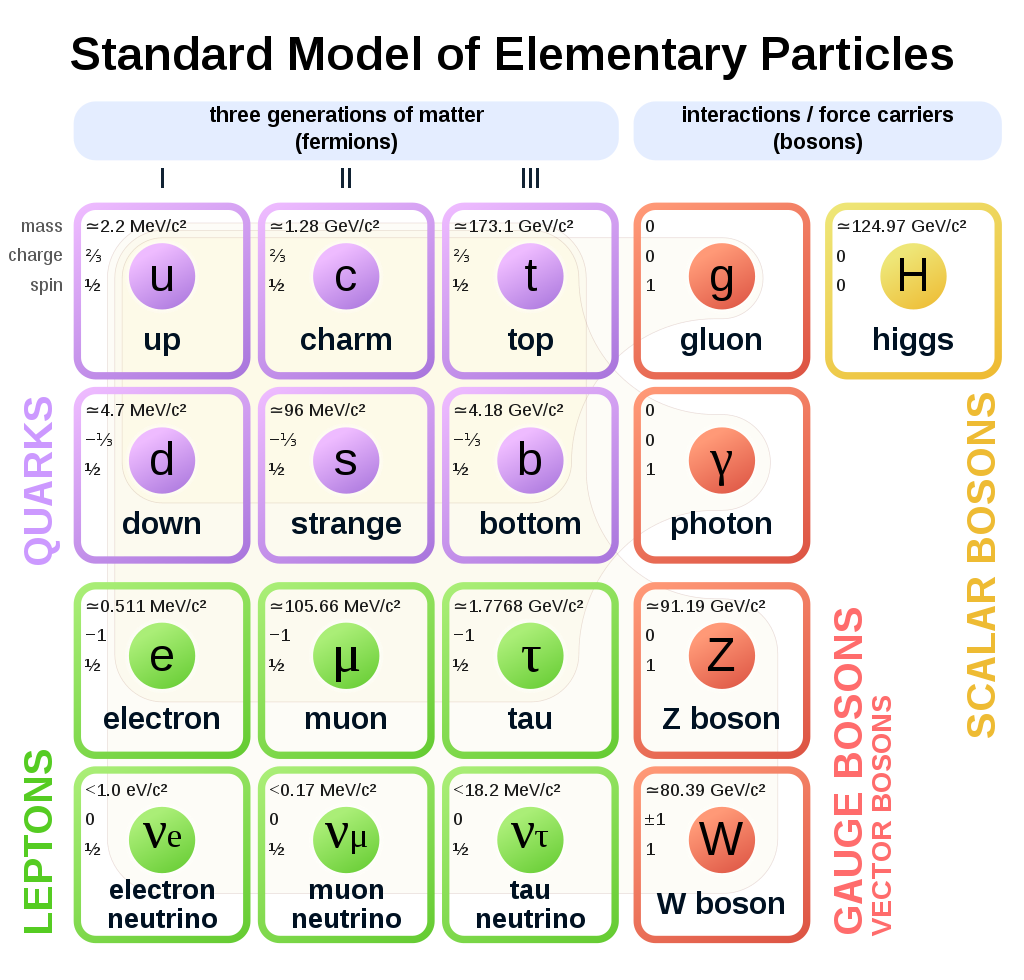
\includegraphics[width=0.55\textwidth]{Figures/01_Introduction/Physics/Standand_model.png}%
\caption{The elementary particle in the standard model.}
\label{fig:standard_model}
\end{figure}


%\textcolor{red}{Discuss more ??? and some texts connecting above and below. }


\subsection{Quark model and QCD}

%\textcolor{red}{Breif history of quark model}

Circa 1950,
the first particle accelerator began to uncover many new particles,
and most of these particles are unstable and decay very quickly,
and hence had not been seen in cosmic ray experiment,
as shown in the Figure.~\ref{fig:particle_zoo}.
With the particle "Zoo" proliferation, 
people suspected that if all these particles are fundamental, 
and W. Lamb joked that he had heard it said that 
"the finder of a new elementary particle used to be rewarded by a Nobel Prize, 
but such a discovery now ought to be punished by a \$10,000 fine."\supercite{Lamb439}
The prosperity of new particles observed from experiments promoted emergence of many new models,
which concocted to try to explain why these particles exit,
such as,
the model of pion composed of nucleons and anti-nucleons from Fermi and Yang\supercite{PhysRev.76.1739},
which was proposed before the discovery of anti-proton.
The quark model was constructed in the early 1960s by M. Gell-Mann and G. Zweig independently to classify scheme for hadrons \supercite{GellMann:1964nj, Zweig:570209},
which gives a natural explanation for isospin and strangeness.
Besides, 
this model predicted the existence of the spin $-3\slash2$ \Omegam,
which is a member of the ground-state decuplet,
and the observation for the this paricle offered a strong evidence of correction of quark model \supercite{PhysRevLett.12.204}.

\begin{figure}[!hbtp]
\centering
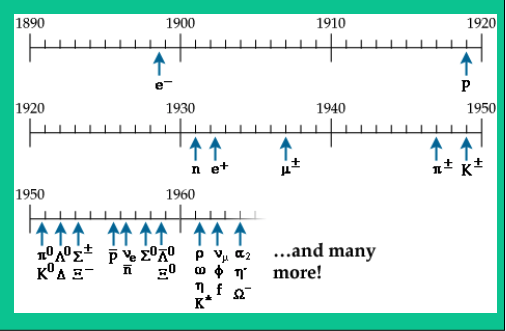
\includegraphics[width=0.65\textwidth]{Figures/01_Introduction/Physics/Particle_Zoo.png}%
\caption{The particle zoo before 1964.}
\label{fig:particle_zoo}
\end{figure}

\subsubsection{Quark model}

The quark model is a description of hadronic properties which strongly emphasizes the role of the minimum-quark-content part of the wave function of hadron\supercite{PDG2020}.
In this model, 
the quarks are strongly interacting fermions with spin $1\slash2$ and positive parity,
while the antiquarks have nagetive parity.
The Table~\ref{tab:quantum_quarks} lists all quantum number of 6 kinds of quarks.
All of them are related with each other through the generalized Gell-Mann-Nishijima formualr:
\begin{equation}
Q = I_z + \frac{\BR + S + C + B + T}{2}
\label{eq:GMN_equation}
\end{equation}
This convension imply the charged meson has the same sign as its charge.
Besides, 
the hypercharge is another useful quantum number, 
which is defined as:
\begin{equation}
	Y = \BR + S -  \frac{C - B + T}{3}
\label{eq:GMN_equation_2}
\end{equation}


\begin{table}[h]
\caption{Some quantum numbers of quarks.}
\begin{center}
	\begin{tabular}{c| cccccc}
\hline \hline
    						&   \dquark  		&  \uquark   		& \squark  			&  \cquark   		&  \bquark   		&   \tquark  \\
\hline 
$Q$(electric charge)   		&   $-\frac{1}{3}$  &   $+\frac{2}{3}$  &   $-\frac{1}{3}$  &   $+\frac{1}{3}$  &   $-\frac{1}{3}$  &   $+\frac{1}{3}$      \\
$I$(isospin)   				&   $\frac{1}{2}$   &   $\frac{1}{2}$   &   $0$ 			&   $0$  			&   $0$  			&   $0$      \\
$I_z$(isospin z-componet) 	&   $\frac{1}{2}$   &   $-\frac{1}{2}$  &   $0$  			&   $0$  			&   $0$  			&   $0$      \\
$S$(strangness)   			&   $0$  			&   $0$  			&   $-1$  			&   $0$  			&   $0$  			&   $0$      \\
$C$(charm)   				&   $0$  			&   $0$  			&   $0$  			&   $+1$  			&   $0$  			&   $0$      \\
$B$(bottomness)   			&   $0$  			&   $0$  			&   $0$  			&   $0$  			&   $-1$  			&   $0$      \\
$T$(topness)   				&   $0$  			&   $0$  			&   $0$  			&   $0$  			&   $0$  			&   $+1$      \\
\BR(baryon)   				&   $\frac{1}{3}$  	&   $\frac{1}{3}$  	&   $\frac{1}{3}$  	&   $\frac{1}{3}$  	&   $\frac{1}{3}$  	&   $\frac{1}{3}$      \\
\hline \hline
\end{tabular}
\normalsize
\label{tab:quantum_quarks}
\end{center}
\end{table}

Quarks are added together to form mesons and baryons using SU(3) group,
and mesons are bound states of quark-antiquark, 
while the baryons are bound states of three quarks.
The properitis of SU(3) tell us the number of the multiplets belonging to product of 3 by 3:
\begin{equation}
	3 \otimes \bar{3} = 1 \oplus 8
\label{eq:meson_3}
\end{equation}
If a fourth quark such as charm \cquark included, 
the SU(3) group can be extended to SU(4), 
and the sixteen mesons are grouped into a 15-plet and a singlet:
\begin{equation}
	4 \otimes \bar{4} = 1 \oplus 15
\label{eq:meson_4}
\end{equation}
And this model can be extended with \bquark included naturally.


The diagram of meson model is very clear and simple, 
and the similar picture can also be extended to baryons.
The "ordinary" baryons are composed of \uquark, \dquark and \squark quarks,
which can be processed in a similar manner to combine three triplets,
namely three representations:
\begin{equation}
	3 \otimes 3 \otimes 3 = 10_{s} \oplus 8_{M,S} \oplus 8_{M,A} \oplus 1_{A}
\label{eq:baryon_3}
\end{equation}
Here $10_{S}$ means symmetric states, 
$8_{M,S}$ and $8_{M,A}$ are mixed symmetry and anti-symmetry combinations respectively,
and $1_{A}$ is a completely anti-symmetric three-quark system,
where the symmetries referred to are under the exchange of any two quarks.


\subsubsection{QCD}

The quark model successfully accommodates all these particles and resonances.
A remarkable success of the $SU(3)_f$ was the prediction, 
including the mass of the $M(\Omegam)=\squark\squark\squark$ baryon\supercite{PhysRevLett.12.204}.
But the model has following problems.
First, 
the most obvious problem is that no matter how hard physicists have tried, 
a free quark has never been observed.
Is the quark a real particle or simply a methematical construct that allows us to keep track to $SU(3)_f$ in an efficient manner.
The second problem is the absence of anti-symmetric combinations of spin and of flavour representations in the baryon sector.
This is not unrelated to a third problem, 
that of Fermi-Dirac statistics.
Baryons, having an odd number of spin-$\frac{1}{2}$ components, 
should have totally anti-symmetric wave-funcitons.
Since they have $L=0$,
their spatial wave-function is symmetric,
and we have imposed that their spin and flavour wave-function factors be symmetric too.
Therefore,
the wave-functions are totally symmetic.

To solve the Fermi-Dirac statistic problem, 
Han and Nambu, Greenberg and Gell-Mann, 
independently proposed adding an additional quantum number to the quarks, 
which is named as "color"\supercite{}.
The Lagrangian of QCD is given by:
\begin{equation}
	\lum = \sum_{q}{\bar{\psi}_{q,a}(i\gamma^{\mu}\partial_{\mu}\delta_{ab}
	-g_{s}\gamma^{\mu}t_{ab}^C}\mathcal{A}_{\mu}^{C}
	-m_{q}\delta_{ab})\psi_{q,b}
	-\frac{1}{4}F_{\mu\nu}^{A}F^{A \mu\nu} 
\label{eq:baryon_3_2}
\end{equation}
where the repeated indices are summed over.
The $\gamma^{\mu}$ are the Dirac $\gamma$-matrixs.
The $\psi_{q,a}$ are quark-field spinors for a quark of flavour $q$ and mass $m_{q}$,
with a color-index $a$ that runs from 1 to 3.
Quarks are said to be in the fundamental representation of the SU(3) color group.
The $\mathcal{A}_{\mu}^{C}$ is the gluon fields,
with $C$ running from 1 to 8,
corresponding to eight kinds of gluon.
The $t_{ab}^C$ represents eight $3\times3$ matrixes and are the generators of SU(3) group,
which illuminates the fact that a gluon's interaction with quark rotates the quark's color in SU(3) space.
The quantity $g_s$ is the QCD coupling constant.
Neither quarks nor gluons are observed as free particles.
Hadrons are color-singlet combination of quarks, anti-quarks, and gluons.
From above formula, 
the fundamental parameters of QCD are the coupling $g_s$ and the quark masses $m_q$.


\begin{figure}[!hbtp]
\centering
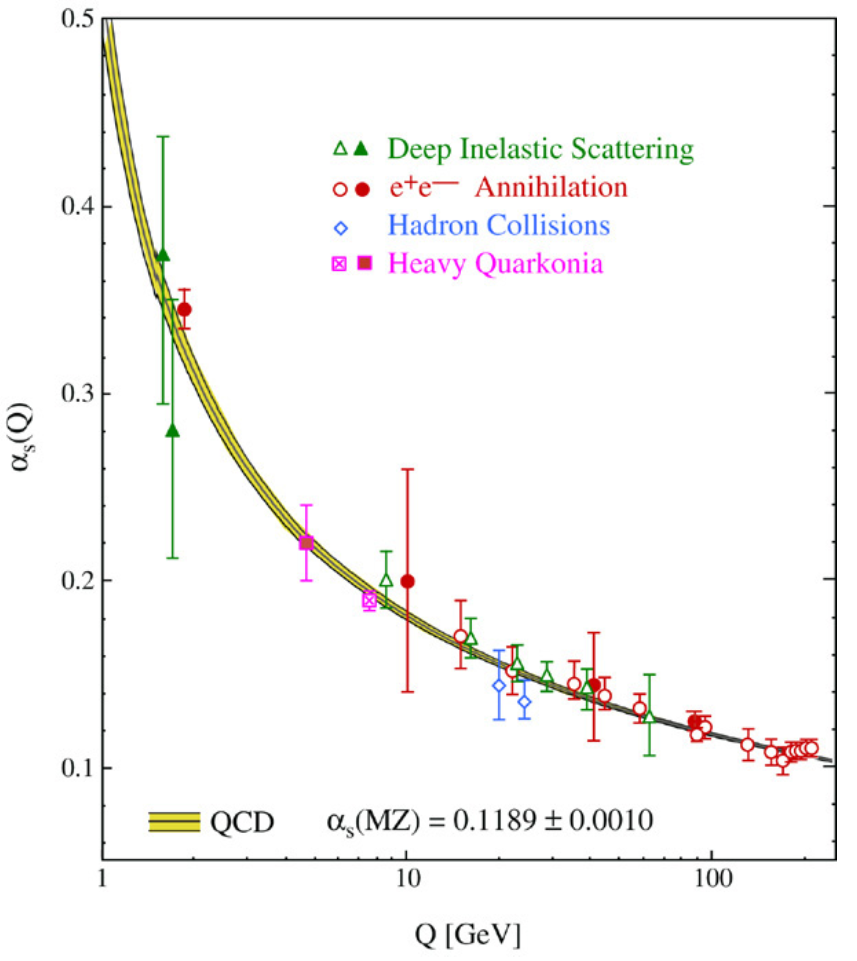
\includegraphics[width=0.45\textwidth]{Figures/01_Introduction/Physics/QCD_asymptotic.png}%
	\caption{Summary of measurements of $\alpha_{s}(Q)$ as a function of hte respective energy scale Q. 
	Figure taken from Ref.~\cite{BETHKE2007351}}
\label{fig:QCD_asymptotic}
\end{figure}


Another intersting phenomenon in QCD is asymptotic freedom,
which leads to a consequence that the strong coupling $\alpha_{s}$ is small enough,
as sufficiently large momentum transfers,
to allow application of perturbation theory in order to provide quantitaive predictions of physical processes.
The strong interaction coupling constant $\alpha_s$ is fundamentally different from the quantum electrodynamics coupling constant,
as not only fermion loops are included in the vertex expansion, 
but also gluon loops, 
owing to the fact that the gluon carry colour charges.
And in QCD,
the gluon-gluon interaction includes additional vacuum polarization diagrams that have virtual gluon loops.
These gluon loops modify the QCD coupling strength $\alpha_s$ in a way that is opposite to QED:
they cause $\alpha_s$ to decrease at short distances and increase at long distances, as shown in Figure.~\ref{fig:QCD_asymptotic} 

%\textcolor{red}{I am not sure if necessary to review more on basic theory. }


\subsubsection{The QCD dilemma}
In QCD,
the component of the standard model of elementary processes that deal with strong interaction,
the elementary particles are color-charged quarks and gluons.
However,
a consequence of confinement is that these particles cannot be seen in experiments.
Although the QCD Lagrangian is expected, 
in priciple,
to completely describe the spectrum of hadrons and all of their properities,
there is no rigorous first-principle translation of this into any useful mathematical expressions.

A fundamental process that can be computed with perturbative QCD is quark-quark elastic scattering at high-momentum transfer.
This shows up in high-energy $pp$ collider experiments as events with two high transverse momentum jets of hadrons 
that are nearly back to back in azimuth. 
The momentum distribution of quarks inside the proton is governed by long-distance QCD 
and approximated by universal parton distribution functions
that are taken from fits to data obtaind from hadron-collider measurements at low center of mass energies,
deep inelastic lepton-proton scattering experiments, etc.
The fundamental QCD $pp\to pp$ process cannot be directly measured,
instead, 
have to be inferred from the jets of hadrons that they produce.
Thus,
even processes that are perturbative QCD calculations involve significant long-distance QCD effects both in the inital and final states.

This nearly total disconnect between the hadrons observed in experiments and the quarks and gluons 
that appear in the theory is a problem of large proportions in paritcle physics.
This is refered as "QCD dilemma".
In addition to the intellectual dissatisfaction with a theory that is not directly applicable to the particles used and detected in experiments,
there is also a practical problem in that many SM tests and searches for new physics (NP) with strong interacting hadrons involved 
in the initial and final states of the associated measurements.
Even experiments without initial or final states that contain hadrons are still subject to their effects from virtual quantum fluctuations.
As a result,
the sensitivities of many NP searching experiments are ultimately limited by hadron-related theoretical uncertainties.
Because of this,
as the experimental sensitivities of NP searches improve,
commensurate improvements of long-distance QCD become more and more important.


A possible way experiments might contribute to these improvements is by identifying patterns in hadron physics
that may help guide the development of improved theoretical models,
and the multi-quark states study offers an unique method to probe QCD. 


\subsection{Multiquark states}

The concept of multiquark resonances came out accompanying with the quark model, 
as G. Zweig\supercite{Zweig:570209} said: 
{\slshape"In general, we would expect that baryons are built not only from product of these aces, 
$AAA$, but also from $\bar{A}AAAA$, 
$\bar{A}\bar{A}AAAAA$", \etc,
where $\bar{A}$ denotes an anti-ace."}
and M. Gell-Mann\supercite{GellMann:1964nj} gave the similar expression:
{\slshape"Baryons can now be constructed from quarks by using the combinations ($qqq$), ($qqqq\bar{q}$), \etc,
while mesons are made of ($q\bar{q}$), ($qq\bar{q}\bar{q}$, \etc)"}.
By then,
many experiments tried to search tetraquark and pentaquark states,
for example,
LEPS Collaboration declared the observation of a narrow $\Theta^{+}(1540)$ paricle,
which is claimed as a pentaquark candidates,
then this state became a hotspot at that time.\supercite{PhysRevLett.91.012002,doi:10.1142/S0217751X04019676}
However, 
this structure was not confirmed from high precise experiments \supercite{doi:10.1142/S0217751X14300208},
and it is not deemed as a genuine resonance now \supercite{PhysRevLett.105.092001}.
The research to $\Theta^{+}(1540)$ told us lessons but also brought us precious experience and opportunities,
so we should not ignore the non-perturbative chromodynamics in spectroscopy study.

A bit of history is mentioned above, 
and current progress about heavy-flavour multiquark study will be reviewed from two perspectives,
experimental evidences and theoretical models in next sections.

%\begin{figure}[!hbtp]
%\centering
%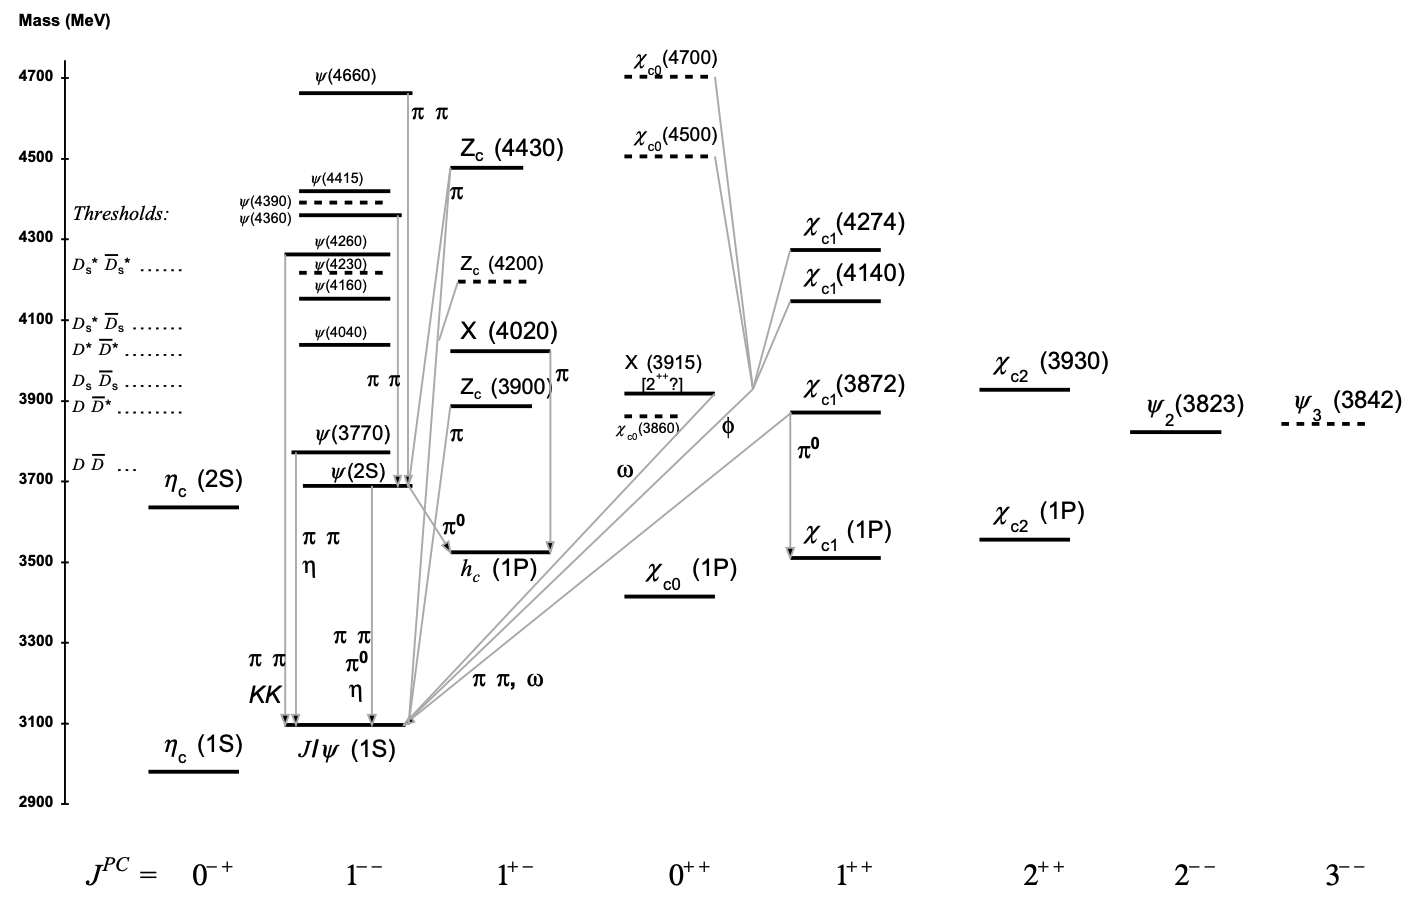
\includegraphics[width=0.8\textwidth]{Figures/01_Introduction/Exotic/charmonium_spect.png}%
%\caption{The level scheme of meson states containing a minimal quark content \cquark\cquarkbar. 
%         The name of a state is determined by its quantum number $I^{G}J^{PC}$.
%	   The arrows indicate the most dominate hadronic transitions.
%	   Taken from Ref.~[\cite{PDG2020}].}
%\label{fig:Charmonium_PDG}
%\end{figure}

The obseverd status of the charmonium-like spectrum are listed in Figure.~\ref{fig:Charmonium_Mod},
which includes the standard charmonium,
non-standard charmonium (tetraquark candidates) and pentaquark candidates.
%The non-standard states have possibility making up of more than two quarks,
%which is also taken as tetraquark candidates.
{\color{red} Maybe to update later, to include 3$P_{c}$, $Z_{cs}$, $T_{cccc}$ and new $X$.}

\begin{figure}[!hbtp]
\centering
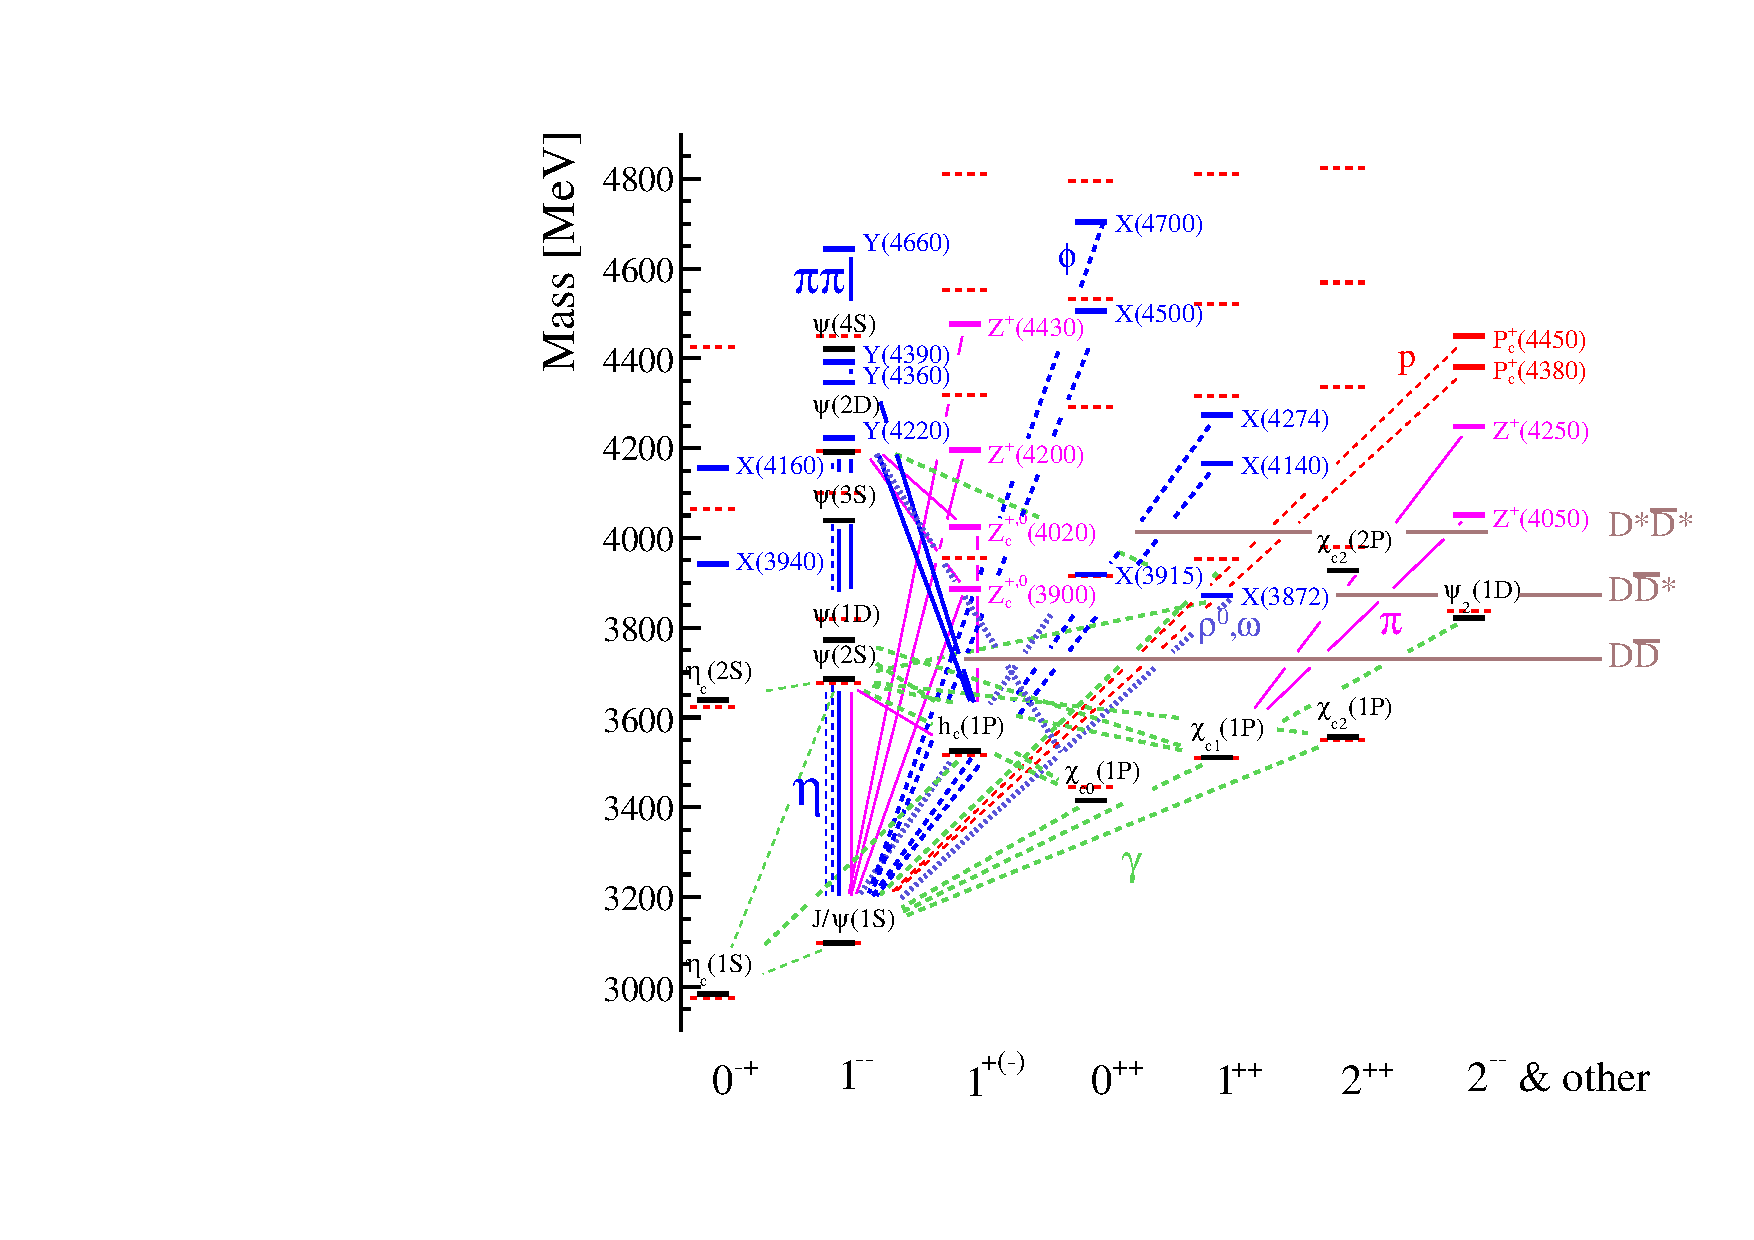
\includegraphics[width=0.8\textwidth]{Figures/01_Introduction/Exotic/charmoniumExotic}%
\caption{The level scheme of meson states containing a minimal quark content \cquark\cquarkbar. 
         The name of a state is determined by its quantum number $I^{G}J^{PC}$.
	   The arrows indicate the most dominate hadronic transitions.
	   Taken from Ref.~[\cite{RevModPhys.90.015003}].}
\label{fig:Charmonium_Mod}
\end{figure}







	%%%%%%%%%%%%%%%%%%%%
%\section{Heavy-flavour multiquark states}

\section{Experimental evidences of heavy-flavour multiquark candidates}
\label{subsection:experimental_introduction}


\subsection{Neutral $X$ and $Y$ multiquark candidates}

\subsubsection{First tetraquark candidate \theX}

The first multiquark candidate is \theX, 
which was observed by Belle Collaboration as a narrow peak in the $\pip\pim\jpsi$ invariant mass distribution 
$B\to K\pip\pim\jpsi$ decays for in 2003\supercite{PhysRevLett.91.262001}.
The invariant mass distribution of $B\to K\pip\pim\jpsi$ is shown in Figure.~\ref{fig:X3872_BELLE},
this resonance is pretty narrow and close to the threshold of the $\D\Dstarb$,
it was popular to be assumed as molecular state,
though the dynamic mechanism is under heated debate today. 
As this state has been discovered more than 16 years, 
and comfirmed in different experiments,
the related studies are pretty fruitful in experimental and theoritical sectors,
some comments about this paritlce will be given below.


\begin{figure}[!hbtp]
\centering
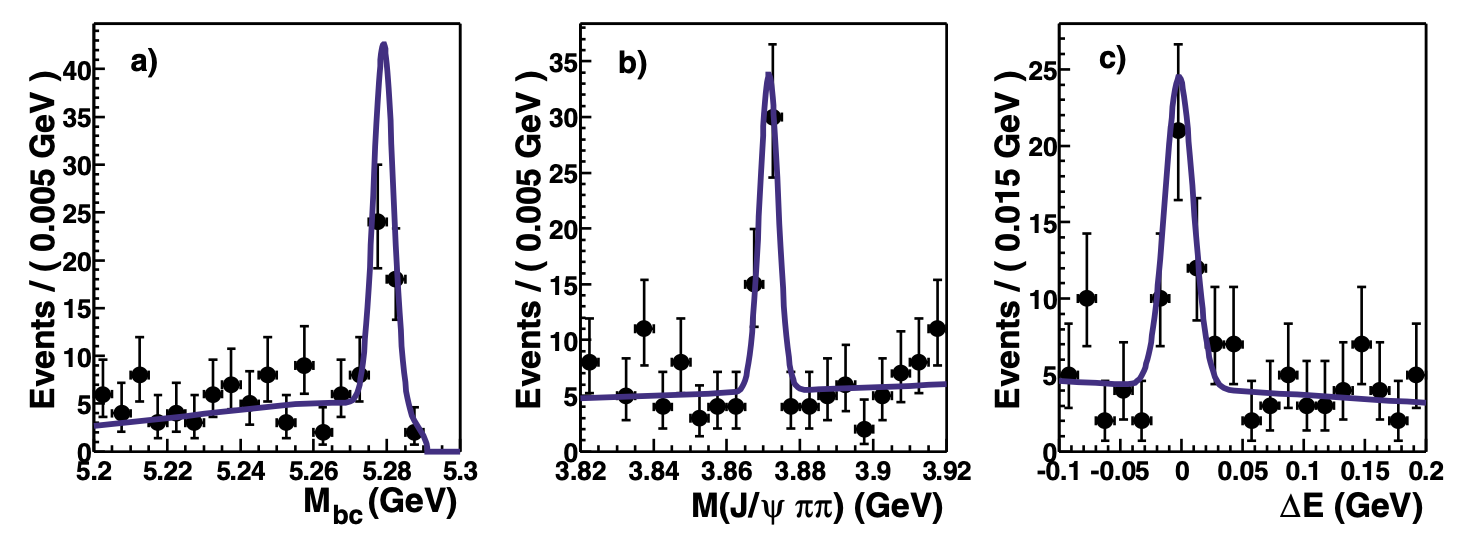
\includegraphics[width=0.9\textwidth]{Figures/01_Introduction/Exotic/X3872_BELLE}%
\caption{Signal-band projections of (a) $M_{bc}$, (b) $\Delta E_{c.m}$ , and (c) $M(\pip\pim\jpsi)$ distributions in
   signal region with the results of the unbinned fit\supercite{PhysRevLett.91.262001}.}
\label{fig:X3872_BELLE}
\end{figure}

The spin and parity of this state were measured by LHCb Collaboration in 2013 with 3\invfb run-I data\supercite{LHCb-PAPER-2013-001}.
5D angular amplitude model was constructed to discribe data,
and likelihood ratio test is performed to discriminate between the $1^{++}$ and $2^{-+}$ assignment.
Based on this technique,
the quantum numbers of \theX are detemined to be $J^{PC}=1^{++}$,
as shown in Figure.~\ref{fig:X3872_spin}.
By a toy simulation method,
the statistical significance of this asssignment can rearch to $16\sigma$.

\begin{figure}[!hbtp]
\centering
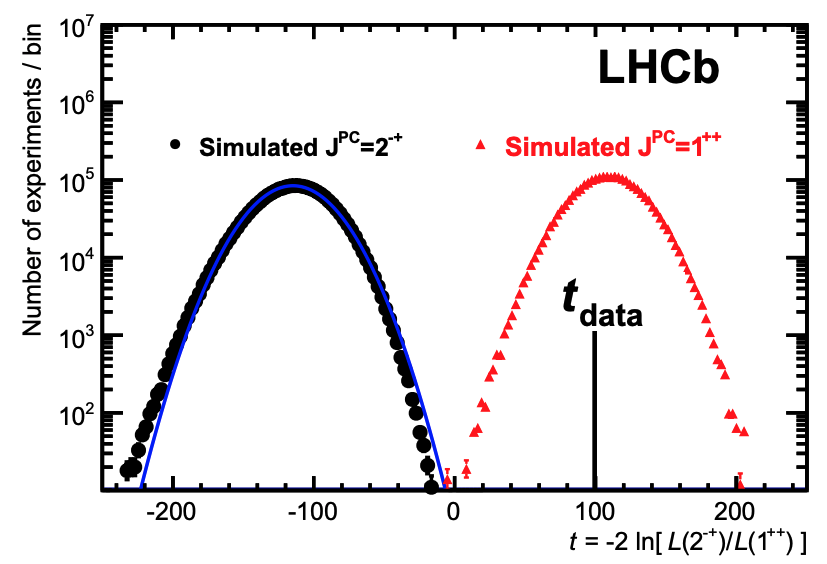
\includegraphics[width=0.6\textwidth]{Figures/01_Introduction/Exotic/X3872_Spin}%
   \caption{ The log-likelihood ratio distribution between $1^++$ and $2^{-+}$ is shown above,
   a Gaussian fit to the $2^{-+}$ distribution is performed\supercite{LHCb-PAPER-2013-001}.}
\label{fig:X3872_spin}
\end{figure}

As the spin and parity of \theX equel to $1^{+}$,
this hadron is also expected as $2^{3}P_{1}$ $c\bar{c}$ state.
However, 
there are still several reasons to classify it as exotic state\supercite{Olsen:2017bmm},
and the apparent evidence is isospin violation in its decay channel $\theX\to\rho\jpsi$.
Since the standard charmonium states contain no constituent \uquark or \dquark,
their isospin number should be 0,
as the $\rho$ is isovector particle, 
the decay mode $\theX\to\rho\jpsi$ should be strongly suppressed due to isospin violation, 
but branching fraction of this decay is nearly equal to the $\theX\to\omega\jpsi$ mode.
In consideration of a kinematic suppression to $\theX\to\omega\jpsi$ by a factor of around 4,
the $I=0$ assignment is favored.

Many explorations to the nature of \theX were performed by different theoretical models\supercite{LIU2019237},
and a good diagnosis to these predictions is to study the relative strength to the $\gamma\psi$ and $\gamma\jpsi$ decay modes.
In the $1^{++}$ charmonium model, 
the $\chicone^{'}$ and $\psi^{'}$ have the same redial wave function,
and $\chicone^{'}\to\gamma\psi^{'}$ transition is more advantageous than that for $\gamma\jpsi$.
In contrast,
in the molecular hypothesis,
the decay to $\gamma\psi^{'}$ is much suppressed\supercite{SWANSON2004189,SWANSON2004197,Dong_2010}.
The evidence for the decay mode $\chicone^{'}\to\gamma\psi^{'}$ was found in 2014, 
and the measured value agrees with expectations of charmonium for pure interpretation of the $\theX$ state
and mixture of charmonium interpretations,
it does not support a pure $\D\Dstarb$ molecular interpretation\supercite{LHCb-PAPER-2014-008}.

Another experimental test to distiguish hypothesis is to measure the prompt production of \theX in high-energy hadron collisions.
If the \theX is a $\D\Dstarb$ state,
its production in the hadron collisions would be more like those of known nuclei stuff, 
rather than those of the $\psi^{'}$\supercite{PhysRevLett.103.162001}.


\subsubsection{$X(3915)$}

After the \theX was observed,
Belle Collaboration studied $B\to K\omega\jpsi$ decay,
and a prominent enhancement appeared in the $\omega\jpsi$ invariant mass distribution near the threshold,
as shown in Figure.~\ref{fig:X3915}(a).
Then,
\babar Collaboration confirmed this result with larger statistic sample,
and the measured mass and width : $M=3915\pm4\mev$ and $\Gamma=31\pm11\mev$,
which are lower values comparing to Belle's measurement\supercite{PhysRevD.82.011101}.
Then,
this state was also observed in the two-photon process $\gamma\gamma\to\omega\jpsi$, 
and the PDG table list the results from both channels\supercite{PDG2020}.

\begin{figure}[!hbtp]
\centering
   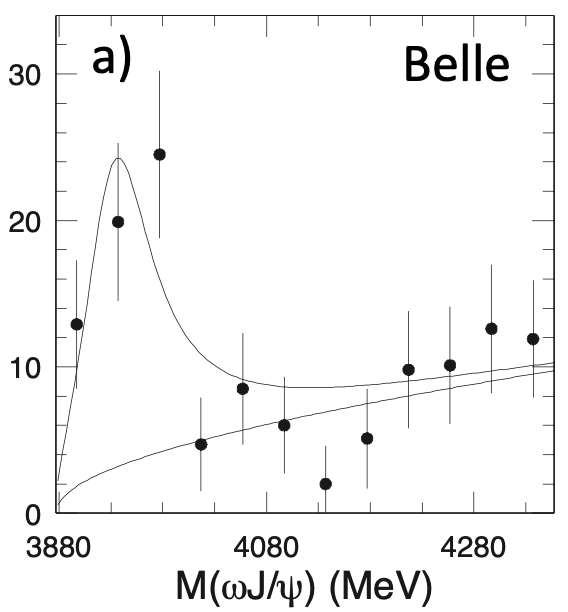
\includegraphics[width=0.32\textwidth]{Figures/01_Introduction/Exotic/X3915_BELLE}%
   %\put(-60,168) {\textrm{\small \bf(a)}}
   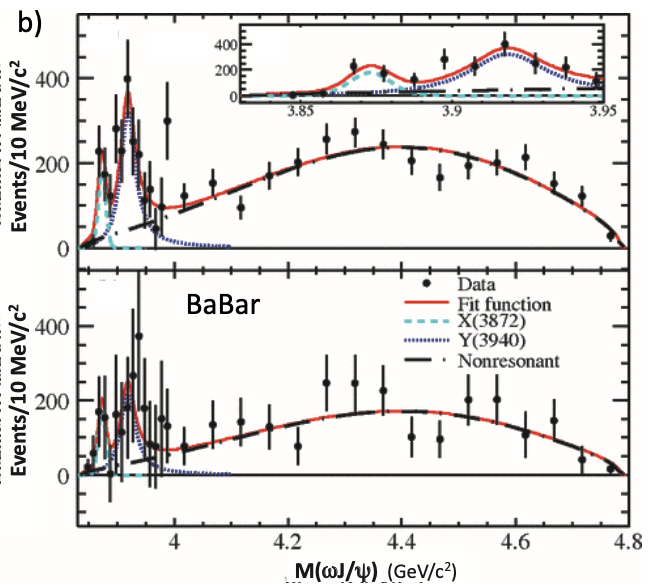
\includegraphics[width=0.4\textwidth]{Figures/01_Introduction/Exotic/X3915_BABAR}%
   %\put(10,168) {\textrm{\small \bf(b)}}
   \caption{ The decay $X(3915)\to\omega\jpsi$ states in $B\to K\omega\jpsi$ decay from \belle\supercite{PhysRevLett.103.162001} (left),
   and \babar\supercite{PhysRevD.82.011101} (right).}
\label{fig:X3915}
\end{figure}

However,
the spin-parity of this state has not been confirmed yet.
With the $\g\g\to\omega\jpsi$ events,
a spin-parity analysis was performed by \babar,
and their study demonstrated that $J^{PC}=0^{++}$ quantum number assignment is favoured.
And from this study,
they thought the $X(3915)$ is a candidate for the $2^{3}\rm{P}_{0}$ charmonium state\supercite{PhysRevLett.104.092001}.
This measured mass of $X(3915)$ is too high for the $2^{3}\rm{P}_{0}$ charmonium state,
which is strongly contradicted with theoretical expectations\supercite{PhysRevD.69.094019,PhysRevD.79.094004}.

Besides,
some people think the $J^{PC}=2^{++}$ hypothesis cannot be ruled out by reanalying from the \babar angular distributions\supercite{PhysRevLett.115.022001}.
However,
$X(3915)=\chi_{c2}^{'}$ is not in accordance with the consquence of $X(3915)$ productiojn in $\Bp\to\Kp\omega\jpsi$ decay.
Since that $\BF(\Bp\to\Kp\chictwo(1\rm{P})) = (1.1\pm0.4)\times10^{-5}$ is much smaller than the branching fraction of:
\begin{equation}
\BF(\Bp\to\Kp X(3915))\times\BF(X\to\omega\jpsi)=3.0^{+0.9}_{-0.7}\times10^{-5}
\label{eq:X_3915_BF}
\end{equation}
In the decay of B-meson to charmonium states, 
the decay widths are expected to be proportional to the square of the $\cquark\cquarkbar$ wave function at the origin,
and decrease with increasing radial quantum number\supercite{PhysRevD.46.R3703}.
The branching fraction measurement is contrary to this model obviously.

The mass of $X(3915)$ is $18.2 \mev$ below the $2m_{\Ds}$ threshold,
and this might mean that it consists of $\cquark\cquarkbar\squark\squarkbar$ component,
or even in a $\Dsp\Dsm$ melecule-like situation.
In the molecular picture,
the $\D\Dbar$ decay would vilolate the OZI-rule\supercite{PhysRevD.59.114027}.
In the $\cquark\cquarkbar\squark\squarkbar$ configuration,
the decay mode least affected by OZI-suppression is $X(3915)\to\eta\etac$ which could be expected to be a dominant decay mode.
However,
\belle saw no significant signal from previous study\supercite{Vinokurova:2015txd}.
The absence of an $\eta\etac$ model would be fatal teh $\cquark\cquarkbar\squark\squarkbar$ quark assignment 
if its partial width was shown to be definately much smaller than that for $\omega\jpsi$ decays.


The $X(3915)$ is one of the most intriguing of the $XYZ$ exotic meson candidates,
however, 
its underlying nature is not fully understood,
and larger data sample of this state is required in the future experiments.
The $J^{P}$ of this state is expected to be detemined from \belletwo,
which have a good ability to reconstruct $\omega$ meson.
Besides,
\lhcb experiment also has potential capacity to probe the $X(3915)$ quantum number,
considering the $\omega$ has been detected in \Bp decay\supercite{LHCb-PAPER-2012-022}.


\subsubsection{$X(4140)$ and other $\jpsi\phi$ states}

Among all known decays of $b-$hadrons,
$\Bp\to\jpsi\phi K^+$ is unique, 
since conventional hadron contributions from kaon excitations (hereafter denoted as $K^{*+}\to\phi K^+$) are broad, 
and visible mass structures on the Dalitz plot are dominated by a number of relatively narrow $X\to\jpsi\phi$ states, 
which are candidates for tetraquarks with hidden-charm and hidden-strangeness. 
Contributions from these exotic hadron components approach half of the entire rate in this decay channel.
The first evidence for the $\jpsi\phi$ state was observed by CDF~\supercite{Aaltonen:2011at},
as shown in the left of Figure.~\ref{newfig3}.
A very narrow ($\Gamma=15.3_{-\phantom{1}6.1}^{+10.4}\pm2.5$\mev), 
near-threshold ($M=4143.4\pm3.0\pm0.6$\mev)
$X(4140)$ state was claimed.
\footnote{The recent PDG\supercite{PDG2020} naming convention calls this state $\chi_{c1}(4140)$. 
However, the generic $X$ label for $\jpsi\phi$ states is used here, 
which is independent of their $J^P$ assignments.}
Such narrow structure was not confirmed by the \belle~\supercite{ChengPing:2009vu}, 
\babar~\supercite{Lees:2014lra}, 
and early low-statistics \lhcb~\supercite{LHCb-PAPER-2011-033} data. 
However, 
the near-threshold state was observed by the \cms collaboration~\supercite{Chatrchyan:2013dma}. 
There was also an evidence for it from the \dzero experiment~\supercite{Abazov:2015sxa},
as shown in the right of Figure.~\ref{fig:D0_4140}.

\begin{figure}[htb]
  \begin{center}
  \vspace{-0.3cm}
   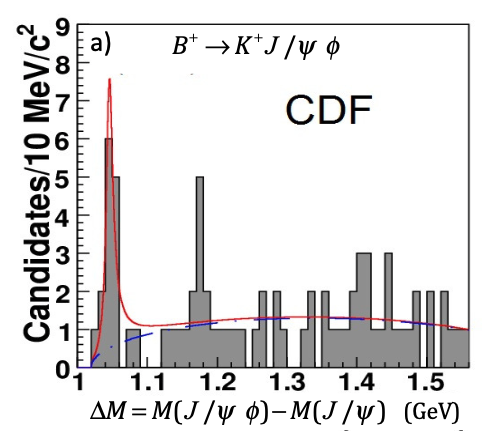
\includegraphics[width=0.41\textwidth]{Figures/01_Introduction/Exotic/neutral_particle/CDF_4140}
   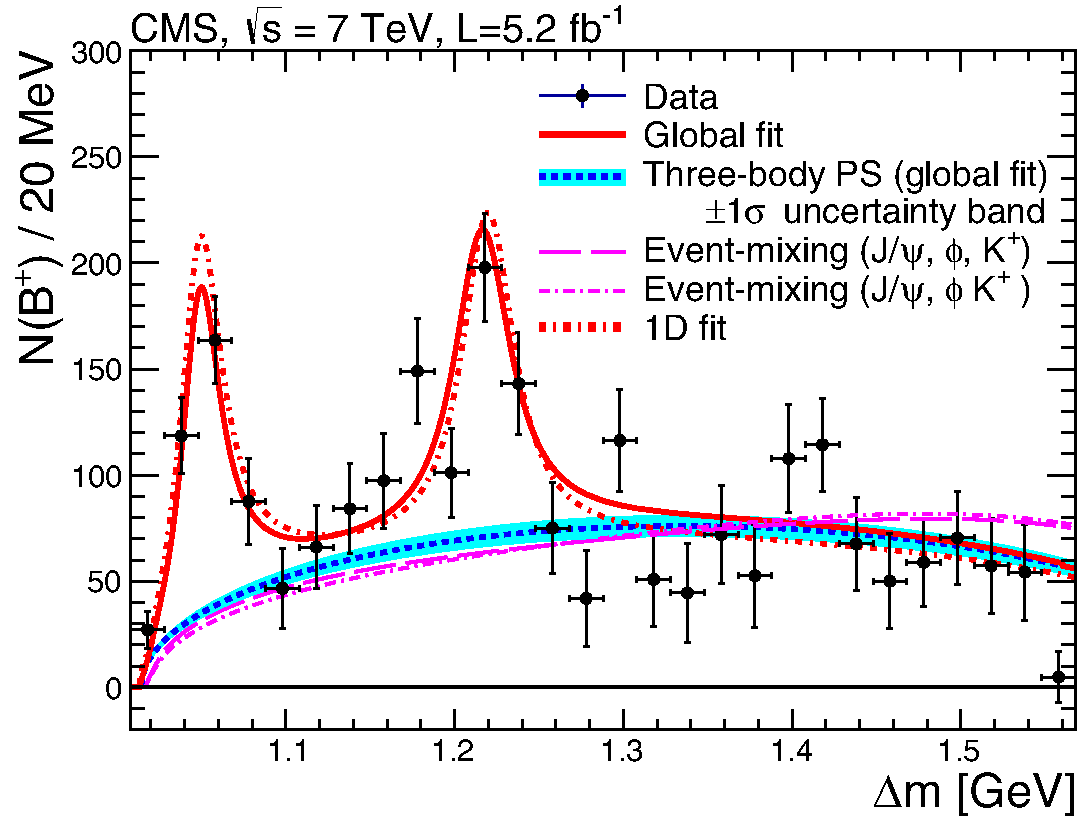
\includegraphics[width=0.48\textwidth]{Figures/01_Introduction/Physics/from_Zcs/newFig3.pdf}
     \vskip -0.4cm
    \caption{\small
     The $\Delta M = M(\jpsi\phi)-M(\jpsi)$ distribution of $\Bp\to\jpsi\phi\Kp$ decays candidates from \cdf experiment in left\supercite{Aaltonen:2011at}; 
     The number of  $\Bp\to\jpsi\phi K^+$  candidates as a function 
     of $\Delta m = m(\mu^+\mu^-\Kp\Km)-m(\mu^+\mu^-)$ at \cms in right\supercite{Abazov:2015sxa}.
    }
    \label{newfig3}
  \end{center}
\end{figure}

\begin{figure}[htb]
  \begin{center}
  \vspace{-0.3cm}
   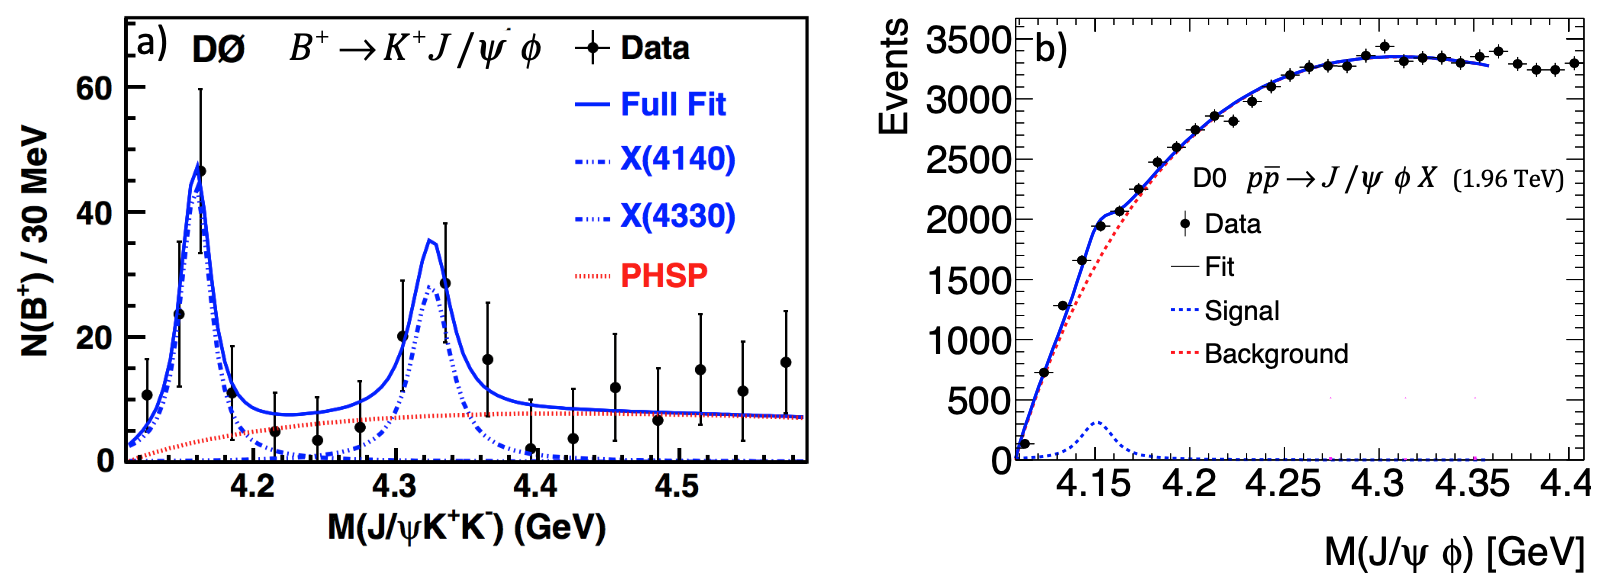
\includegraphics[width=0.91\textwidth]{Figures/01_Introduction/Exotic/neutral_particle/D0_4140}
     \vskip -0.4cm
    \caption{\small
     The $\Delta M = M(\jpsi\phi)-M(\jpsi)$ distribution of $\Bp\to\jpsi\phi\Kp$ decays candidates from \cdf experiment in left\supercite{Aaltonen:2011at}; 
     The number of  $\Bp\to\jpsi\phi K^+$  candidates as a function 
     of $\Delta m = m(\mu^+\mu^-\Kp\Km)-m(\mu^+\mu^-)$ at \cms in right\supercite{Abazov:2015sxa}.
    }
    \label{fig:D0_4140}
  \end{center}
\end{figure}

An evidence for a second structure, $X(4274)$, in the \cdf\supercite{Aaltonen:2011at} and \cms\supercite{Chatrchyan:2013dma} was observed.
%The \cdf collaboration presented $3.1 \sigma$ evidence for a second relatively narrow $\jpsi\phi$ mass peak around $4274\pm8 \mev$\supercite{}.
The $\jpsi\phi$ mass distribution among $2480\pm160$ $\Bp\to\jpsi\phi K^+$ events detected by \cms is shown in right of Figure.~\ref{newfig3}, 
which was obtained after the subtraction of a very large combinatorial background.
There is also hint of the second structure near $4274 \mev$ in the $\jpsi\phi$ mass distribution at \dzero,
as shown in the left of Figure.~\ref{fig:D0_4140},
with a small significance around $1.7 \sigma$. 
Besides,
\belle reported a $3.2 \sigma$ evidence of a narrow $\jpsi\phi$ peak around $4351 \mev$,
and the corresponding $J^P$ assignment is $0^{++}$ or $2^{++}$.
However, there is no obvious $X(4140)$ evidence in the same sample\supercite{PhysRevLett.104.112004}.


\lhcb~\supercite{LHCb-PAPER-2016-018,LHCb-PAPER-2016-019} performed the first amplitude analysis of $\Bp\to\jpsi \phi K^+$ decays,
by investigating the $\jpsi \phi$ structures in Run 1 data.
The number of $\Bp\to\jpsi \phi K^+$ signal events was $4289\pm141$ with a background fraction of $23\%$.
The data can be described by including seven $K^{*+}\to\phi K^+$ resonances,
which are determined by the fit and consistent with either known or predicted states,
besides, 
four $X\to\jpsi\phi$ structures and non-resonant $\phi K^+$ and $\jpsi \phi$ also contribute.
The mass projections of $\phi K^+$ and $\jpsi \phi$ combinations are shown in Figure.~\ref{fig:defmasses}.
%Table~\ref{tab:run1} shows the results, including the determined masses, widths, fit fractions and spin-parity assignments.
The four $X$ structures and a non-resonant $\jpsi\phi$ contribution all had significance above 5$\sigma$.
The existence of $\Xtwo$ was established.

\begin{figure}[hbtp]
  \begin{center}
    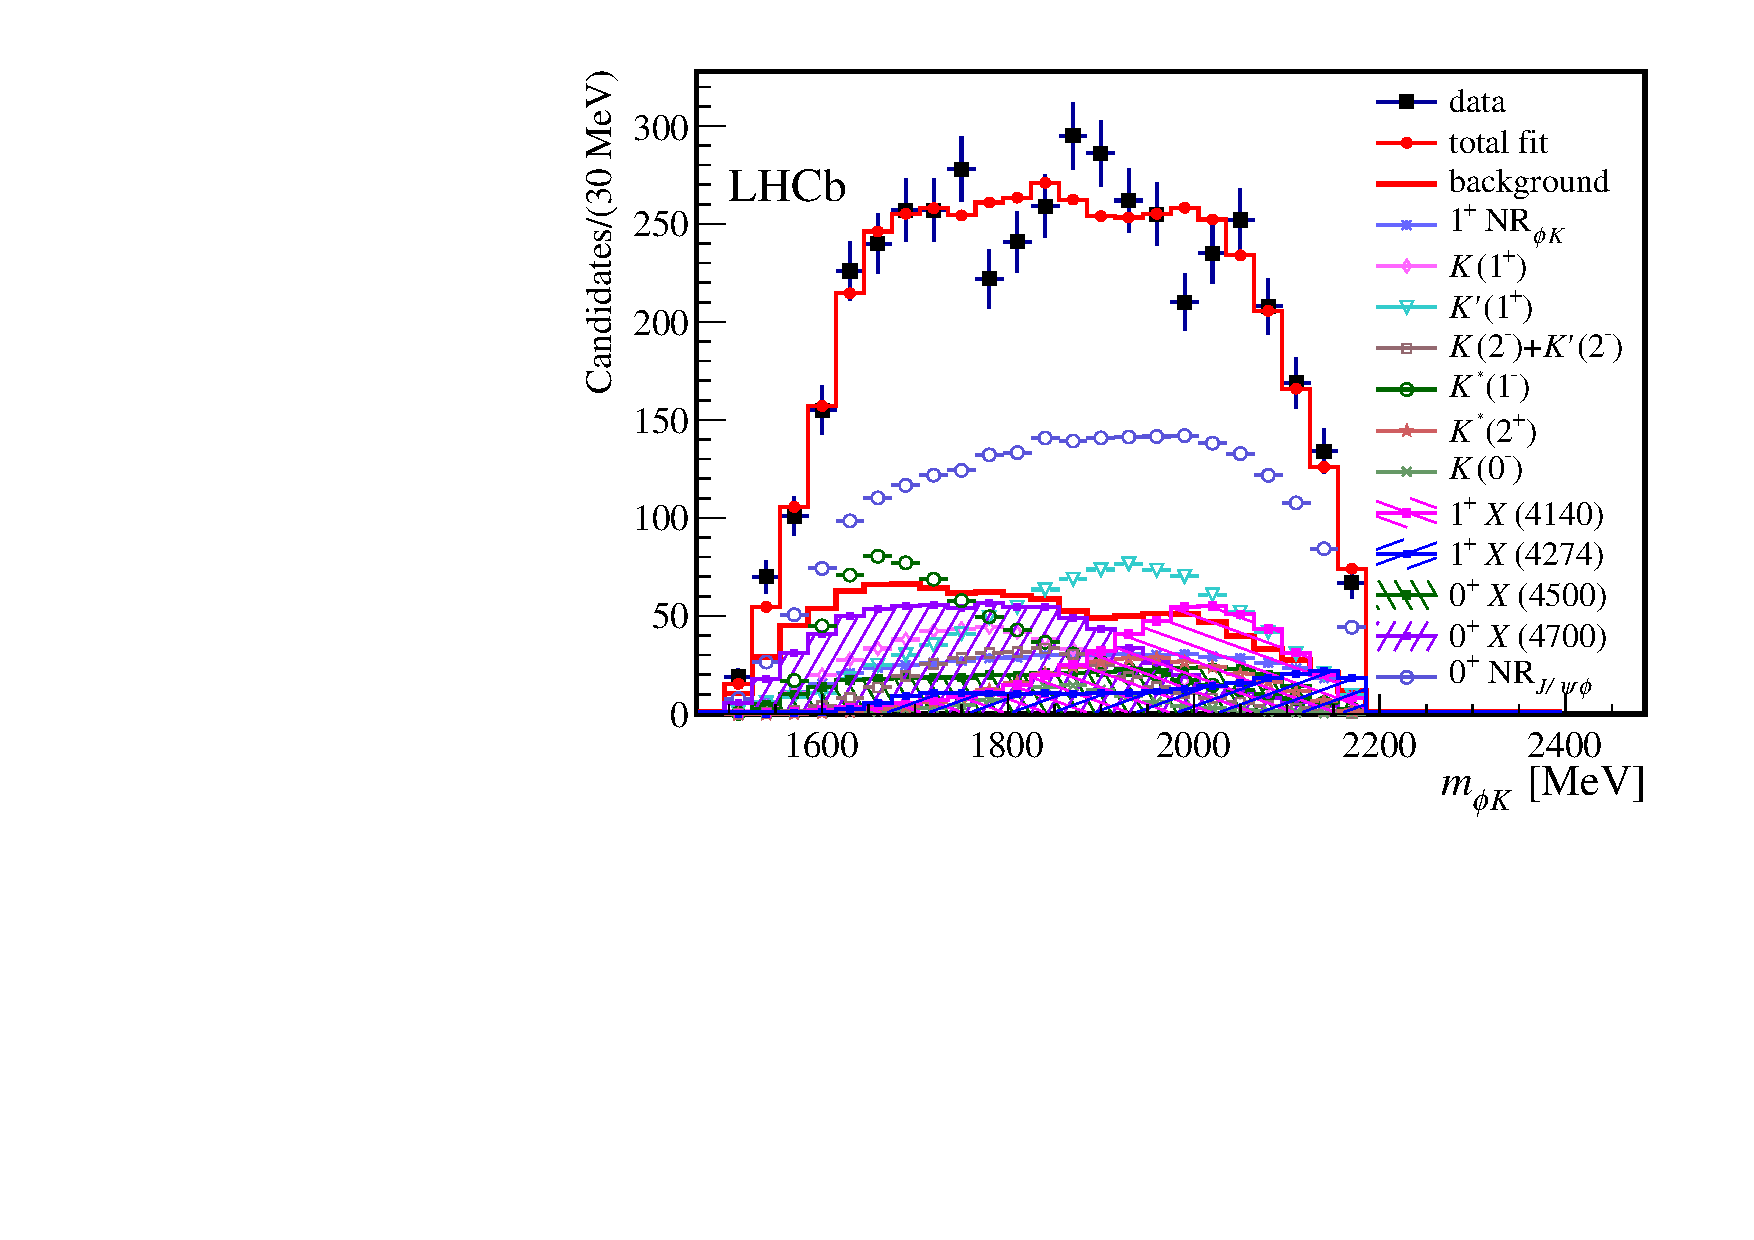
\includegraphics[width=0.5\textwidth]{Figures/01_Introduction/Physics/from_Zcs/newbase_PhiKh.pdf}%
    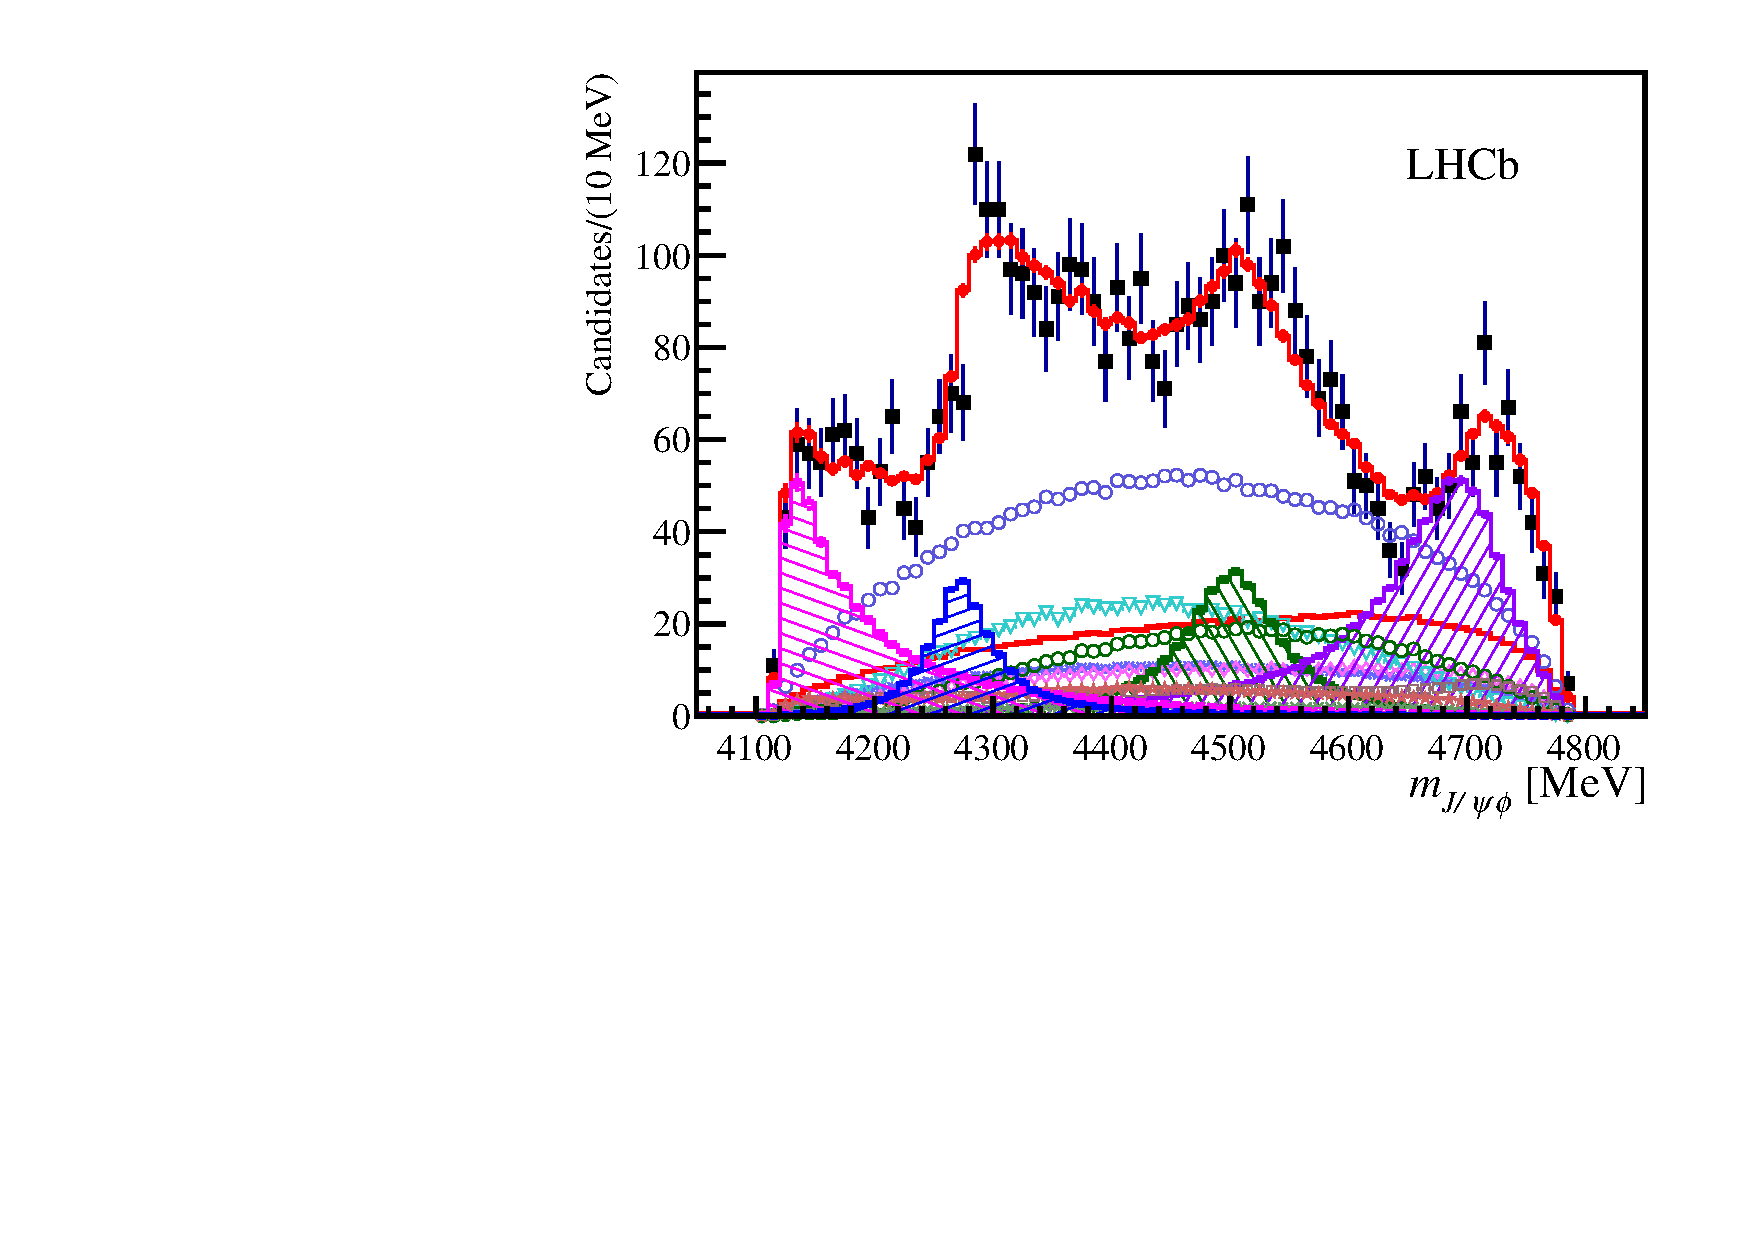
\includegraphics[width=0.5\textwidth]{Figures/01_Introduction/Physics/from_Zcs/newbase_JpsiPhih.pdf}
  \end{center}
\caption{
    Distributions of $\phi K^+$ (left) and $\jpsi\phi$ (right)
    invariant masses for the $\Bp\to\jpsi \phi K^+$ candidates (black data points)
    compared with the results of the default amplitude fit
    to the Run 1 data \supercite{LHCb-PAPER-2016-018}.}
  \label{fig:defmasses}
\end{figure}

The $J^{P}$ quantum numbers of $\Xone$ are determined to be $1^{++}$.
Besides,
the $\Xtwo$ state were identified as $1^{++}$ at  $>5\sigma$ significance,
while the $\Xthree$ and $\Xfour$ states as $0^{++}$ at $>4\sigma$. 
Actually,
the $1^{++}$ quantum number for $\Xone$ and $\Xtwo$ rule out the $0^{++}$ or $2^{++}$ $\Dss\Dssm$molecular models
%\supercite{PhysRevD.80.017502,PhysRevD.80.054019,Zhang_2010,PhysRevD.80.114013,ALBUQUERQUE2009186,Wang:2009ry,Ding:2009vd}.
\supercite{PhysRevD.80.017502,PhysRevD.80.054019,PhysRevD.80.114013,ALBUQUERQUE2009186,Wang:2009ry,Ding:2009vd}.
Besides,
some people suggested $\Xone$ structure is kinematically induced cusp\supercite{PhysRevD.91.034009,KARLINER2016365}.
No proposed molecular bound-state or cusp model can account for these $\Xtwo J^{PC}$ values. 
A hybrid charmonium state in this mass region would have $J^{PC}=1^{-+}$\supercite{MAHAJAN2009228}.
An exception is a tetraquark model implemented by Stancu\supercite{Stancu_2010},
states that not only correctly assigned $1^{++}$ to the $\Xone$, 
but also predicted a second $1^{++}$ state at a mass that is not much higher than that of the $\Xtwo$.
The $\Xthree$ and the $\Xfour$ have been suggested as candidates for the $\chiczero(4P)$ and $\chiczero(5P)$ states, 
since they lie in the predicted mass and width ranges for these states\supercite{PhysRevD.94.074007,PhysRevD.94.114018}.
However,
none of the \jpsi structures observed in B decays are consistent with the state seen in two-photon collisions by the Belle collaboration.\supercite{PhysRevLett.104.112004}

Notably, the $\Xone$ width was substantially larger than previously determined,
while the mass is consistent with the $\Xone$ values from \cdf and \cms. 
In the spectroscopy study,
a one-dimensional fit to a mass distribution for a resonance peak might lead to biased mass and width.
Besides, 
a one-dimensional fit might underestimate systematic error,
due to the given assumption about the background shape and its incoherence\supercite{RevModPhys.90.015003}.


\begin{table*}[bht]
%\scriptsize  
\caption{Results related to the $X(4140)\to\jpsi\phi$ mass peak,
first observed in $B^+\to\jpsi\phi K^+$ decays.
The first (second) significance quoted for Ref.~[\cite{Abazov:2015sxa}]
is for the non-prompt (prompt) production components (the mass and width were determined from the non-prompt sample).
The last column gives a fraction of $B^+\to\jpsi\phi K^+$ rate
attributed to the $X(4140)$ structure, however, the CDF and
D0 results were normalized to a $B^+\to\jpsi\phi K^+$ rate
that excluded the high $\jpsi\phi$ mass range.
}
\label{tab:x4140}
\hbox{
\hbox{
\renewcommand{\arraystretch}{1.2}
\def\1#1{\multicolumn{1}{c}{#1}}
%\def\2{\ifthenelse{\boolean{prl}}{\quad}{}}
\def\2{}
%\def\3{\ifthenelse{\boolean{prl}}{}{\!\!\!}}
%\def\pms{\ifthenelse{\boolean{prl}}{\pm}{\!\pm\!}}
\begin{tabular}{cllcl}
\hline
%Year & Experiment  & \1{$B\to\jpsi\phi K$} & \multicolumn{4}{c}{$X(4140)$ peak} \\
%     & luminosity  & \1{yield}             & \1{Mass [MeV]} & \1{Width [MeV]} & \1{Significance} & \1{Fraction \%} \\
     {$B\to\jpsi\phi K$} & \multicolumn{4}{c}{$X(4140)$ peak} \\
     {yield}   & {Mass [\mev]} & {Width [\mev]} & {Significance} & {Fraction \%} \\

\hline\hline
2008 &  \multicolumn{3}{l}{\cdf 2.7 fb$^{-1}$  \cite{Aaltonen:2009tz} }\\ \hdashline
$58\pm10$ \2 &
$4143.0\pm2.9\pm1.2$ {\quad} &
$11.7\,^{+8.3}_{-5.0}\pm3.7$ &
$3.8\sigma$ & \\ \hline
%\hline
{\it 2009} & \multicolumn{3}{l}{ {\it \belle} \cite{Brodzicka:2010zz} } \\ \hdashline
$\mathit{325\pm21}$  &
$\mathit{4143.0}$ {\it fixed} &
$\mathit{11.7}$ {\it fixed} &
$\mathit{1.9\sigma}$ & \\ \hline
%\hline
{\it 2011} & \multicolumn{3}{l} { {\it \cdf 6.0 fb$^{-1}$}  \cite{Aaltonen:2011at} }  \\ \hdashline
$\mathit{115\pm12}$  &
$\mathit{4143.4\,^{+2.9}_{-3.0}\pm0.6}$ &
$\mathit{15.3\!^{+10.4}_{-6.1}\pm2.5}$ &
$\mathit{5.0\sigma}$ &
$\mathit{14.9\pm3.9\pm2.4}$ \\ \hline
%\hline
2011 & \multicolumn{3}{l} {\lhcb 0.37 fb$^{-1}$  \cite{LHCb-PAPER-2011-033} }  \\ \hdashline
$346\pm20$  &
$4143.4$ fixed &
$15.3$ fixed   &
$1.4\sigma$    &
$<7$ @~90\%CL \\ \hline
%\hline
2013 & \multicolumn{3}{l} { \cms 5.2 fb$^{-1}$  \cite{Chatrchyan:2013dma} } \\ \hdashline
$2480\pm160$ &
$4148.0\pm2.4\pm6.3$ &
$28^{+15}_{-11}\pm19$ &
$5.0\sigma$ &
$10\phantom{.0}\pm3$ (stat.)  \\ \hline
%\hline
2013 & \multicolumn{3}{l} {\dzero 10.4 fb$^{-1}$  \cite{Abazov:2013xda} } \\ \hdashline
$215\pm37$  &
$4159.0\pm4.3\pm6.6$ &
$19.9\pm12.6\,^{+1.0}_{-8.0}$ &
$3.0\sigma$ &
$21\phantom{.0}\pm8\phantom{.0}\pm4$ \\ \hline
%\hline
2014 & \multicolumn{3}{l} { \babar  \cite{Lees:2014lra} } \\ \hdashline
$189\pm14$  &
$4143.4$ fixed &
$15.3$ fixed  &
$1.6\sigma$ &
$<13.3$ @~90\%CL \\ \hline
%\hline
2016 & \multicolumn{3}{l} { \lhcb 3.0 fb$^{-1}$  \cite{LHCb-PAPER-2016-018,LHCb-PAPER-2016-019} } \\ \hdashline
$4289\pm151$  &
$4146.5\pm4.5\,^{+4.6}_{-2.8}$ &
$83\pm21^{+21}_{-14}$  &
$8.4\sigma$    &
$13.0\pm3.2\,^{+4.8}_{-2.0}$ \\ \hline
%\hline
2021 & \multicolumn{3}{l} {\lhcb 9.0 fb$^{-1}$ Chapter.~\ref{chap:Zcs_study} } \\ \hdashline
$24220\pm170$  &
$4118\pm11\,^{+19}_{-36}$ &
$162\pm21^{+24}_{-49}$  &
$13\sigma$    &
$17\pm3\,^{+19}_{-6}$ \\ \hline
\hline
2015 & \multicolumn{3}{l} {\dzero 10.4 fb$^{-1}$  \cite{Abazov:2015sxa} } \\ \hdashline
{$p\bar{p}\to\jpsi\phi...$} &
$4152.5\pm1.7\,^{+6.2}_{-5.4}$ &
$16.3\pm5.6\pm11.4$ &
$5.7\sigma$ ($4.7\sigma$){\hskip-1cm\quad} &
 \\
\hline
\end{tabular}
}
}
\end{table*}





\begin{table*}[bht]
\caption{Results related to $\jpsi\phi$ mass structures
heavier than the $X(4140)$ peak.
The unpublished results are shown in italics.
The last column gives a fraction of the total $B^+\to\jpsi\phi K^+$ rate
attributed to the given structure.
}
\label{tab:x4274plus}
\hbox{
%\hbox{\ifthenelse{\boolean{prl}}{}{\quad\hskip-2.2cm}
\hbox{
%\ifthenelse{\boolean{prl}}{}{\begin{footnotesize}}
\def\1#1{\multicolumn{1}{c}{#1}}
\def\2{}
%\def\3{\ifthenelse{\boolean{prl}}{}{\!\!\!}}
%\def\pms{\ifthenelse{\boolean{prl}}{\pm}{\!\pm\!}}
\renewcommand{\arraystretch}{1.2}
\begin{tabular}{cllcl}
\hline
%Year & Experiment  & \1{$B\to\jpsi\phi K$} & \multicolumn{3}{c}{$X(4274-4351$) peaks(s)} \\
%     & luminosity  & \1{yield}        & \1{Mass [MeV]} & \1{Width [MeV]} & Significance  & \1{Fraction [\%]} \\
{$B\to\jpsi\phi K$} & \multicolumn{4}{c}{$X(4274-4351$) peaks(s)} \\
{yield}             & \1{Mass [MeV]} & \1{Width [MeV]} & Significance  & \1{Fraction [\%]} \\
\hline\hline
{\it 2011} & \multicolumn{4}{l}{ {\it CDF 6.0 fb$^{-1}$}  \cite{Aaltonen:2011at} } \\ 
$\mathit{115\pm12}$ &
$\mathit{4274.4\,^{+8.4}_{-6.7}\pm1.9}$ &
$\mathit{32.3{^{+21.9}_{-15.3}}\!\pm7.6}$ &
$\mathit{3.1\sigma}$ & \\ \hline
%\hline
2011 & \multicolumn{4}{l} { \lhcb 0.37 fb$^{-1}$  \cite{LHCb-PAPER-2011-033} } \\ \hdashline
$346\pm20$ &
$4274.4$ fixed &
$32.3$ fixed  &
& $<\phantom{0}8$ @~90\%CL \\ \hline
%\hline
2013 & \multicolumn{4}{l} { CMS 5.2 fb$^{-1}$  \cite{Chatrchyan:2013dma}  } \\ \hdashline
$2480\pm160$ &
$4313.8\pm5.3\pm7.3$ &
$38\phantom{.0}\,^{+30\phantom{.0}}_{-15\phantom{.0}}\pm16$ &
& \\ \hline
%\hline
2013 & \multicolumn{4}{l} { D0 10.4 fb$^{-1}$  \cite{Abazov:2013xda} } \\ \hdashline
$215\pm37$ \2 &
$4328.5\pm12.0$ &
$30\phantom{.0}$ fixed &
  & \\ \hline
%\hline
2014 & \multicolumn{4}{l} { \babar \cite{Lees:2014lra} } \\ \hdashline
$189\pm14$  &
$4274.4$ fixed &
$32.3$ fixed  &
$1.2\sigma$  &
$<18.1$ @~90\%CL \\ \hline
%\hline
2016 & \multicolumn{4}{l} { \lhcb 3.0 fb$^{-1}$  \cite{LHCb-PAPER-2016-018,LHCb-PAPER-2016-019} } \\ \hdashline
$4289\pm151$  &
$4273.3\pm8.3\,^{+17.2}_{-\phantom{1}3.6}$ &
$56\phantom{.0}\pm11\phantom{.0}\,^{+\phantom{1}8}_{-11}$  &
$6.0\sigma$    &
$7.1\pm2.5\,^{+3.5}_{-2.4}$ \\
                &
$4506\phantom{.3}\pm11\phantom{.0}\,^{+12}_{-15}$ &
$92\phantom{.0}\pm21\phantom{.0}\,^{+21}_{-20}$  &
$6.1\sigma$    &
$6.6\pm2.4\,^{+3.5}_{-2.3}$ \\
                &
$4704\phantom{.3}\pm10\phantom{.0}\,^{+14}_{-24}$ &
$120\pm31\phantom{.0}\,^{+42}_{-33}$  &
$5.6\sigma$    &
$12\phantom{.0}\pm5\phantom{.0}\,^{+9\phantom{.0}}_{-5\phantom{.0}}$ \\ \hline
%\hline
2021 & \multicolumn{4}{l} { \lhcb 9.0 fb$^{-1}$  Chapter.~\ref{chap:Zcs_study} } \\ \hdashline
$24220\pm170$  &
$4294\pm4\,^{+3}_{-6}$ &
$53\pm5\pm5$  &
$18\sigma$    &
$2.8\pm0.5\,^{+0.8}_{-0.4}$ \\
                &
$4474\pm3\pm3$ &
$77\pm6^{+10}_{-8}$  &
$20\sigma$    &
$5.6\pm0.7^{+2.4}_{-0.6}$ \\
                &
$4684\pm7^{+13}_{-16}$ &
$126\pm15^{+37}_{41}$  &
$15\sigma$    &
$7.2\pm1.0^{+4.0}_{-2.0}$ \\
                &
$4694\phantom\pm4^{+16}_{-3}$ &
$87\pm8^{+16}_{-3}$  &
$17\sigma$    &
$8.9\pm1.2^{+4.9}_{-1.4}$ \\

\hline
2010 & \multicolumn{4}{l} { \belle \cite{PhysRevLett.104.112004} } \\ \hdashline
\1{$\gamma\gamma\to\jpsi\phi$} &
$4350.6\,^{+4.6}_{-5.1}\pm0.7$ &
$13\,^{+18}_{-\phantom{0}9}\pm4$ &
$3.2\sigma$ & \\
\hline
\end{tabular}
%\ifthenelse{\boolean{prl}}{}{\end{footnotesize}}
}
}
\end{table*}

The experimental results about $\jpsi\phi$ structures are summarized in Table.~\ref{tab:x4140} and Table.~\ref{tab:x4274plus},
which are updated from the tables shown in Ref.~[\cite{Olsen:2017bmm}].
The lastest results based on \lhcb Run 1 and Run 2 samples are also included,
which are also partial conclusions in Chapter.~\ref{chap:Zcs_study} of this dissertation.
It is possibily that the $\jpsi\phi$ structures are derived from molecular model or cusp effect,
the mass thresholds of $\Ds\Dsm$, 
with S-wave $J^P$ values, 
are shown in Table~\ref{tab:mt1}.
It is found that only the $X(4140)$ is close to the thresholds and have the S-wave $J^P$ consistent with the determinations from the amplitude fit. 
Higher values of angular momentum are expected to be suppressed for threshold effects.


\begin{table}[h]
%\scriptsize
\begin{center}
\scriptsize
\caption{Mass threshold and S-wave $J^P$ of $\Ds\Dsm$ containing $\ccbar\ssbar$.}
\label{tab:mt1}
\begin{tabular}{|c|c|c|c|c|c|c|}

\hline
L=0                                                    &\tabincell{c}{$0^-$ \Dsp \\ (1968\mev)}
&\tabincell{c}{$1^-$ \Dssp \\ (2112\mev)}              &\tabincell{c}{$0^+$ $D^{*+}_{s0}$ \\ (2318\mev)}
&\tabincell{c}{$1^+$ $D^{+}_{s1}$ \\ (2460\mev)}       &\tabincell{c}{$1^+$ $D^{+}_{s1}$ \\ (2536\mev)}
&\tabincell{c}{$2^+$ $D^{*+}_{s2}$ \\ (2573\mev)}  \\
\hline
\tabincell{c}{$0^-$ \Dsm \\ (1968\mev)}                &\tabincell{c}{$0^+$ \\(3926\mev)}
&{\color{red}{\tabincell{c}{ $1^+$ \\ (4080\mev)} } }  &\tabincell{c}{$0^-$ \\(4286\mev)}
&\tabincell{c}{$1^-$\\ (4428\mev)}  & \tabincell{c}{$1^-$\\ (4504\mev)}
&\tabincell{c}{$2^-$\\ (4541\mev)}    \\
\hline
\tabincell{c}{$1^-$ \Dssm \\ (2112\mev)}               &-
&\tabincell{c}{$(0,1,2)^+$ \\(4224\mev)}         &\tabincell{c}{$1^-$\\ (4430\mev)}
&\tabincell{c}{$(0,1,2)^-$ \\(4572\mev)}         &\tabincell{c}{$(0,1,2)^-$\\ (4648\mev)}
&\tabincell{c}{$(1,2,3)^-$\\ (4685\mev)}  \\
\hline
\tabincell{c}{$0^+$ $D^{*-}_{s0}$ \\(2318\mev)}       &-
&-                                                     &\tabincell{c}{$0^+$ \\(4636\mev)}
&\tabincell{c}{$1^+$ \\(4778\mev)}   &\tabincell{c}{$1^+$\\ (4854\mev)}
&\tabincell{c}{$2^+$\\ (4891\mev)}  \\
\hline
\tabincell{c}{$1^+$ $D^{-}_{s1}$ \\(2460\mev)}       &-
&-                                                     &-
&\tabincell{c}{$(0,1,2)^+$ \\(4920\mev)}   &\tabincell{c}{$(0,1,2)^+$\\ (4996\mev)}
&\tabincell{c}{$(1,2,3)^+$\\ (5033\mev)}  \\
\hline
\tabincell{c}{$1^+$ $D^{-}_{s1}$ \\(2536\mev)}       &-
&-                                                     &-
&-                                            &\tabincell{c}{$(0,1,2)^+$\\ (5072\mev)}
&\tabincell{c}{$1^+$\\ (5109\mev)}  \\
\hline
\tabincell{c}{$2^+$ $D^{*-}_{s2}$ \\(2573\mev)}       &-
&-                                                     &-
&-                                &-
&\tabincell{c}{$(0,1,2,3,4)^+$\\ (5146\mev)}  \\
\hline

\end{tabular}
\end{center}
\end{table}



\subsubsection{$X$ states in $\ep\en$ collision }

\begin{figure}[!hbtp]
\centering
   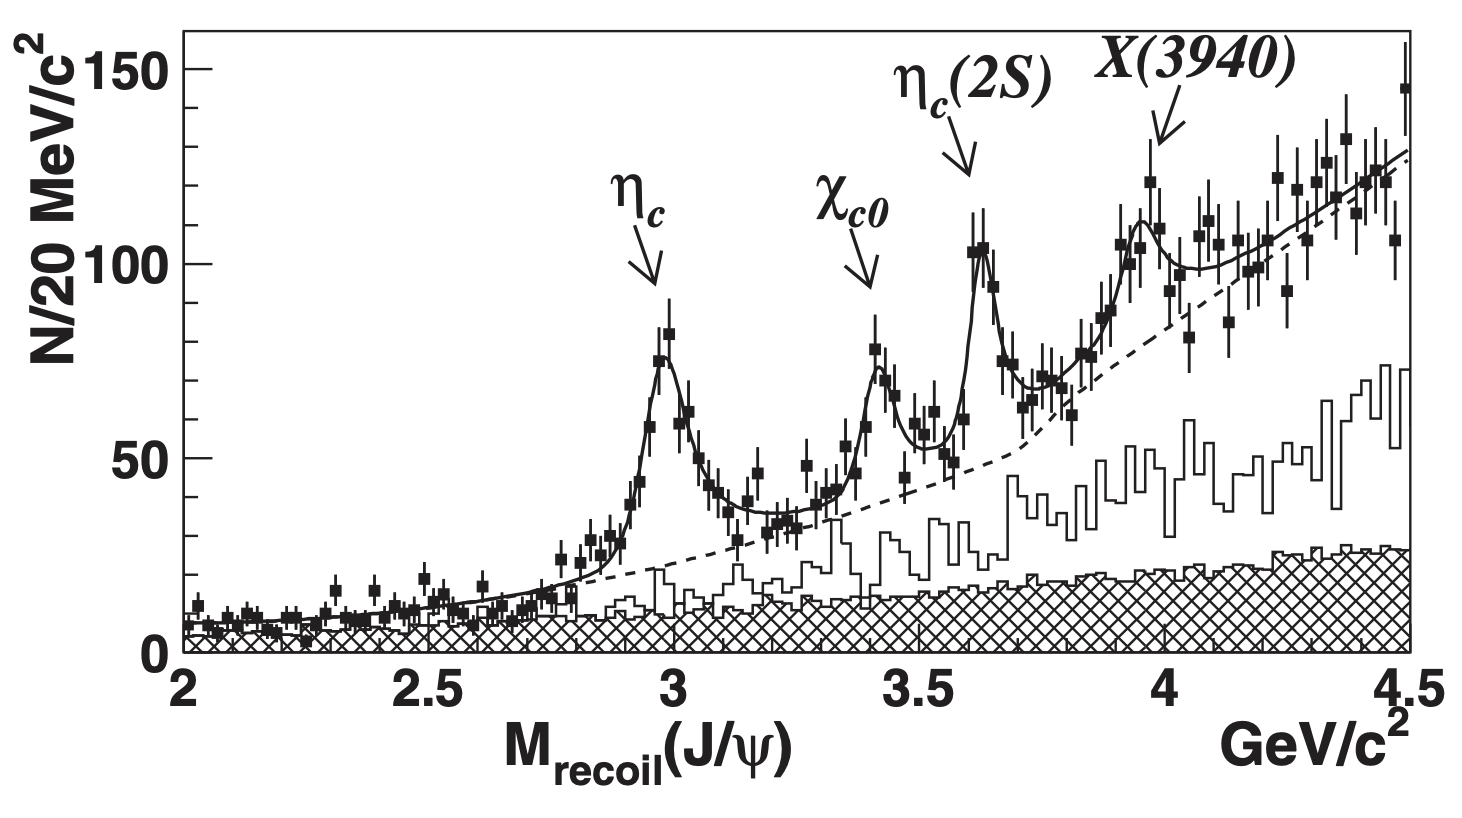
\includegraphics[width=0.6\textwidth]{Figures/01_Introduction/Exotic/neutral_particle/X3940} \\%
   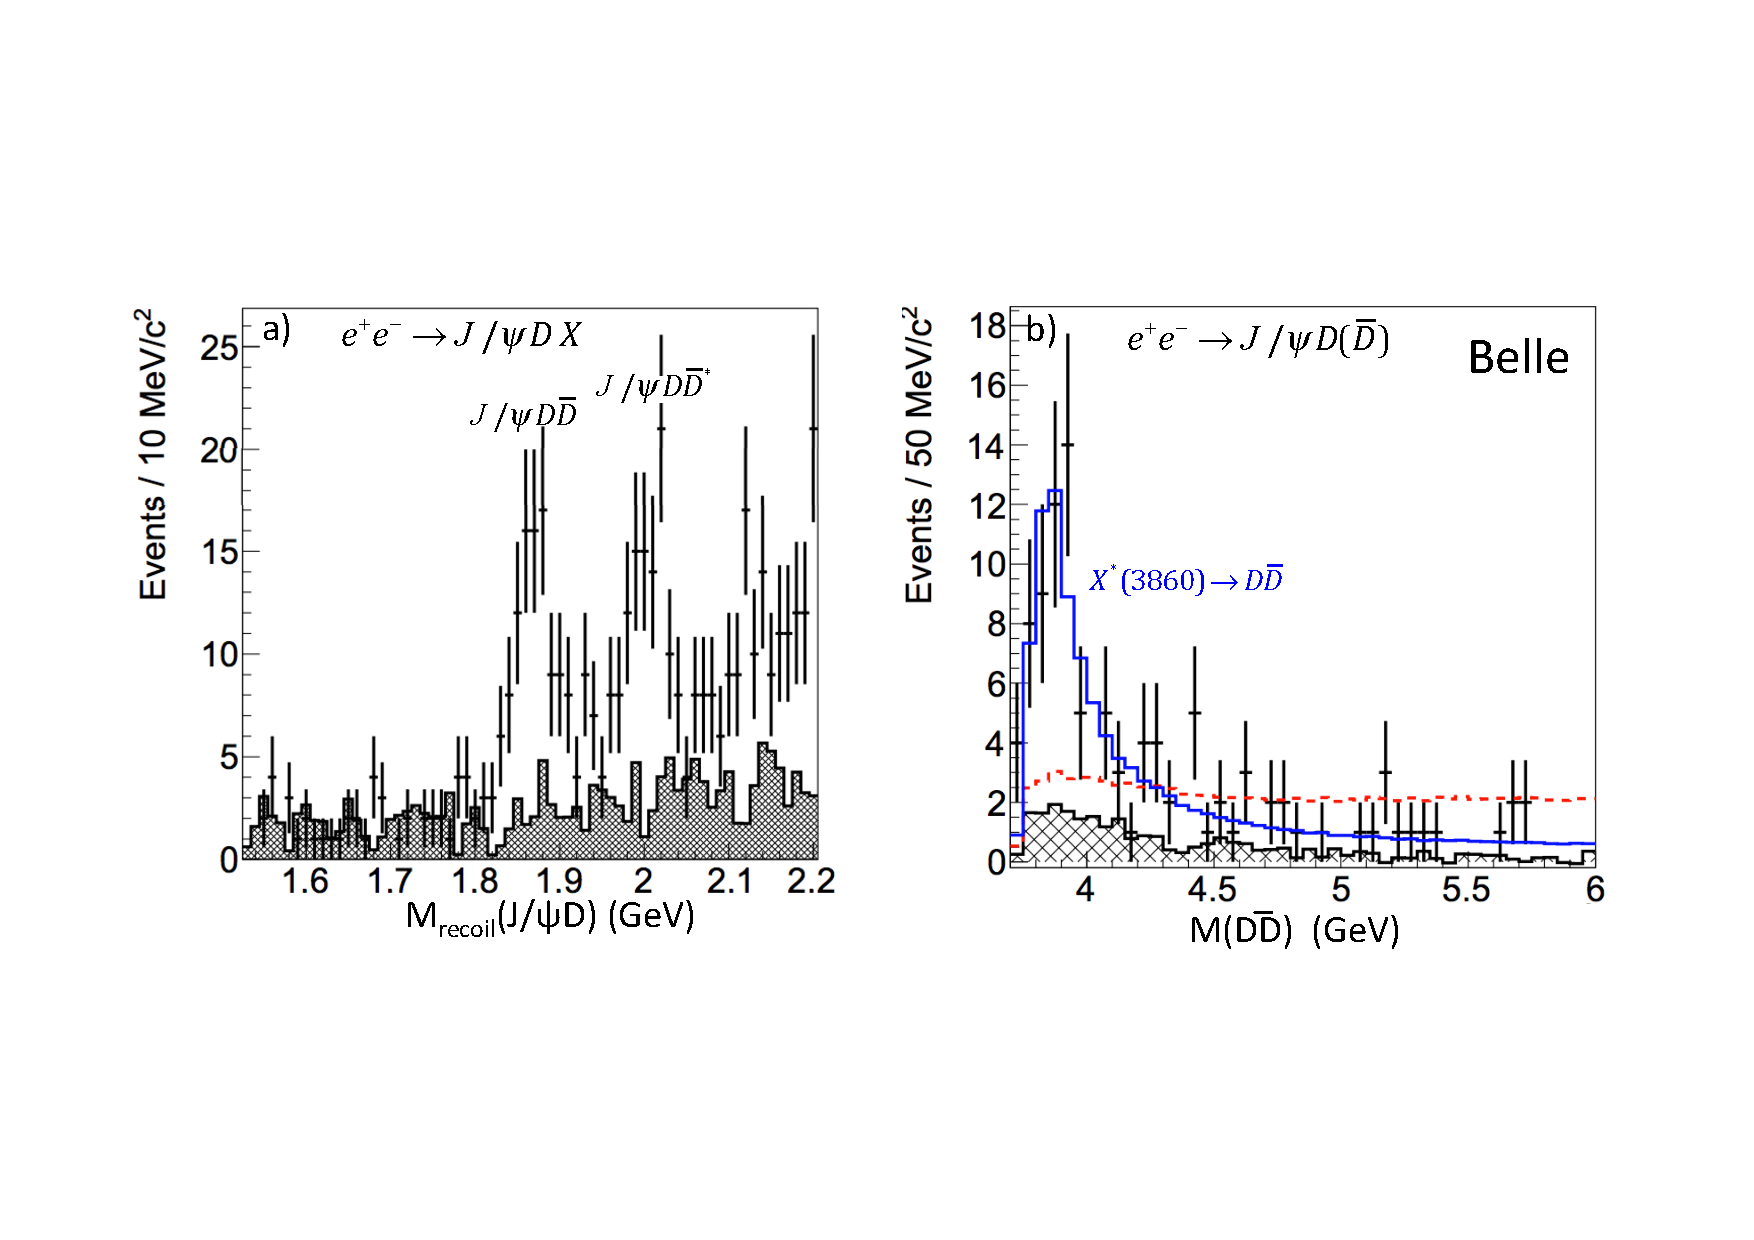
\includegraphics[width=0.8\textwidth]{Figures/01_Introduction/Exotic/neutral_particle/belle_x3860} %
   \caption{ The distribution of masses recoiling from the \jpsi at \belle\supercite{PhysRevLett.98.082001} (above).
   The distribution of masses recoiling from a reconstructed \jpsi and D-meson in $\ep\en\to\jpsi\D X$ annihilation (bottom left) 
   and $\D\Dbar$ invariant mass distribution (bottom right)\supercite{PhysRevLett.100.202001}. }
\label{fig:X3940}
\end{figure}

Three X states, $X^{*}(3860)$, $X(3940)$ and $X(4160)$, are introduced in this section,
which are not observed in any B-meson decay channel. 
The first is $X(3940)$,
which was first seen at \belle in 2007\supercite{PhysRevLett.98.082001}.
According to the distribution of masses recoiling against a \jpsi in inclusive $\ep\en\to\jpsi X$ annihilation,
four peaks appear clearly, 
as shown in Figure.~\ref{fig:X3940} above.
The fourth peak is named as $X(3940)$, 
as is not associated with any known or expected charmonium. 
Besides,
this peak was also observed in the $\D\Dstarb$ invariant mass distribution for $\ep\en\to\jpsi DX$ events\supercite{PhysRevLett.100.202001}.
At the same energy point,
\belle observed the $X(4160)$ structure in $\D\Dbar$ invariant mass distribution for exclusive $\ep\en\to\jpsi\Dstar\Dstarb$\supercite{PhysRevLett.100.202001}.
%as shown in the bottom right of Figure.~\ref{fig:X3940}.
The $J^{P}$ of $X(3940)$ and $X(4160)$ are $0^{-+}$ possibily according to these measurements by \belle.
In consideration of the masses of these two states are far below expectations for the $0^{-+}$ charmonium,
$X(3940)$ and $X(4160)$ are taken as tetraquark candidates.
The bottom left plot of Figure.~\ref{fig:X3940} shows the distribution of masses masses recoiling against a detected \jpsi and \D meson in $\ep\en\to\jpsi\Dp X$ annihilation events collected in \belle\supercite{PhysRevD.95.112003},
while The bottom right plot of Figure.~\ref{fig:X3940} shows $\D\Dbar$ invariant mass distribution for the exclusive $\ep\en\to\jpsi\D\Dbar$ events.
From an amplitude fit, 
$X(3862)$ structure is very significant and $J^{PC}=0^{++}$ quantum number assignment gives the best fit.
This state is considered as $\chiczero(2P)$ charmonium state now.





\subsubsection{$Y$ states with $J^{PC}=1^{--}$}
\label{subsub:Y4260}

\begin{figure}[!hbtp]
\centering
   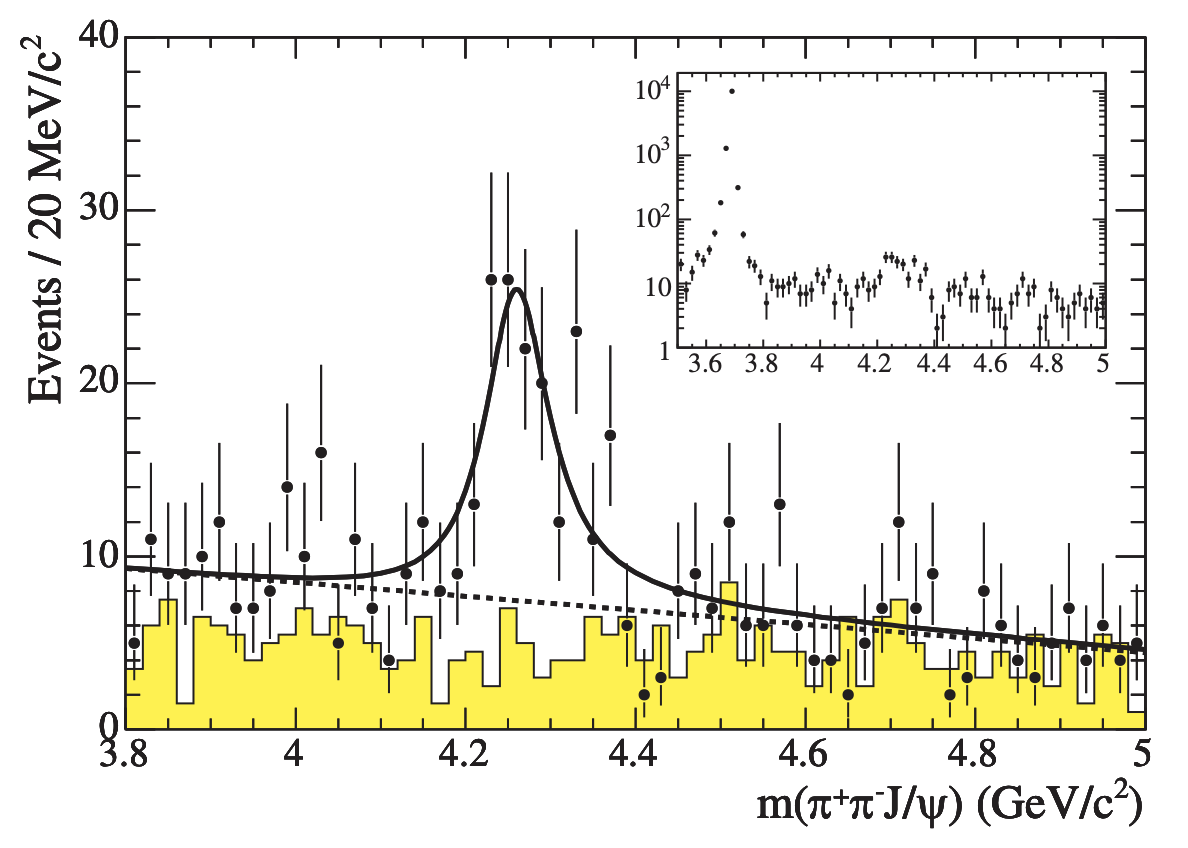
\includegraphics[width=0.5\textwidth]{Figures/01_Introduction/Exotic/neutral_particle/X4260} \\%
   \caption{ The $\jpsi\pip\pim$ invariant mass distribution in the process $\ep\en\to\g\pip\pim\jpsi$ at \babar\supercite{PhysRevD.71.052001}.}
\label{fig:Y4260}
\end{figure}

The \babar group considered to search the possible $1^{--}$ state in the $\ep\en\to\g\pip\pim\jpsi$ process after the $X(3872)$ was discovered in \belle.
No structrue around $3872 \mev$ appeared.
However,
an unexpected strong accumulation of events in $\jpsi\pip\pim$ invariant masses distribtion have a peak near $4260 \mev$\supercite{PhysRevD.71.052001},
as shown in Figure.~\ref{fig:Y4260}.
This observation is confirmed very quickly by \cleo\supercite{PhysRevLett.96.162003} and \belle\supercite{PhysRevLett.99.182004}.

Afterwards,
\babar observed another peak around 4320 \mev\supercite{PhysRevLett.98.212001},
as shown in the left of Figure.~\ref{fig:Y4360}.
Then, 
\belle confirmed this state with a larger data sample \supercite{PhysRevLett.99.142002},
as shown in the right of Figure.~\ref{fig:Y4360}.
As the mass peak is near $4360 \mev$,
finally, it is named as $Y(4360)$.
\besiii performed a data scan between $E_{cm}=3882 \mev$ and $4567 \mev$ later \supercite{PhysRevLett.118.092001} ,
with "high luminosity" and "low luminosity" scans respectively,
as shown in Figure.~\ref{fig:bes_Y4260}.
It is obvious that the line shape cannot be well described by a single Breit-Wigner function,
then the fit was performed  using two BW amplitude by \besiii,
and the corresponding masses of two resonances are $4222\pm4 \mev$ and $4320\pm13 \mev$,
which were explained as $Y(4260)$ and $Y(4360)$.


\begin{figure}[!hbtp]
\centering
   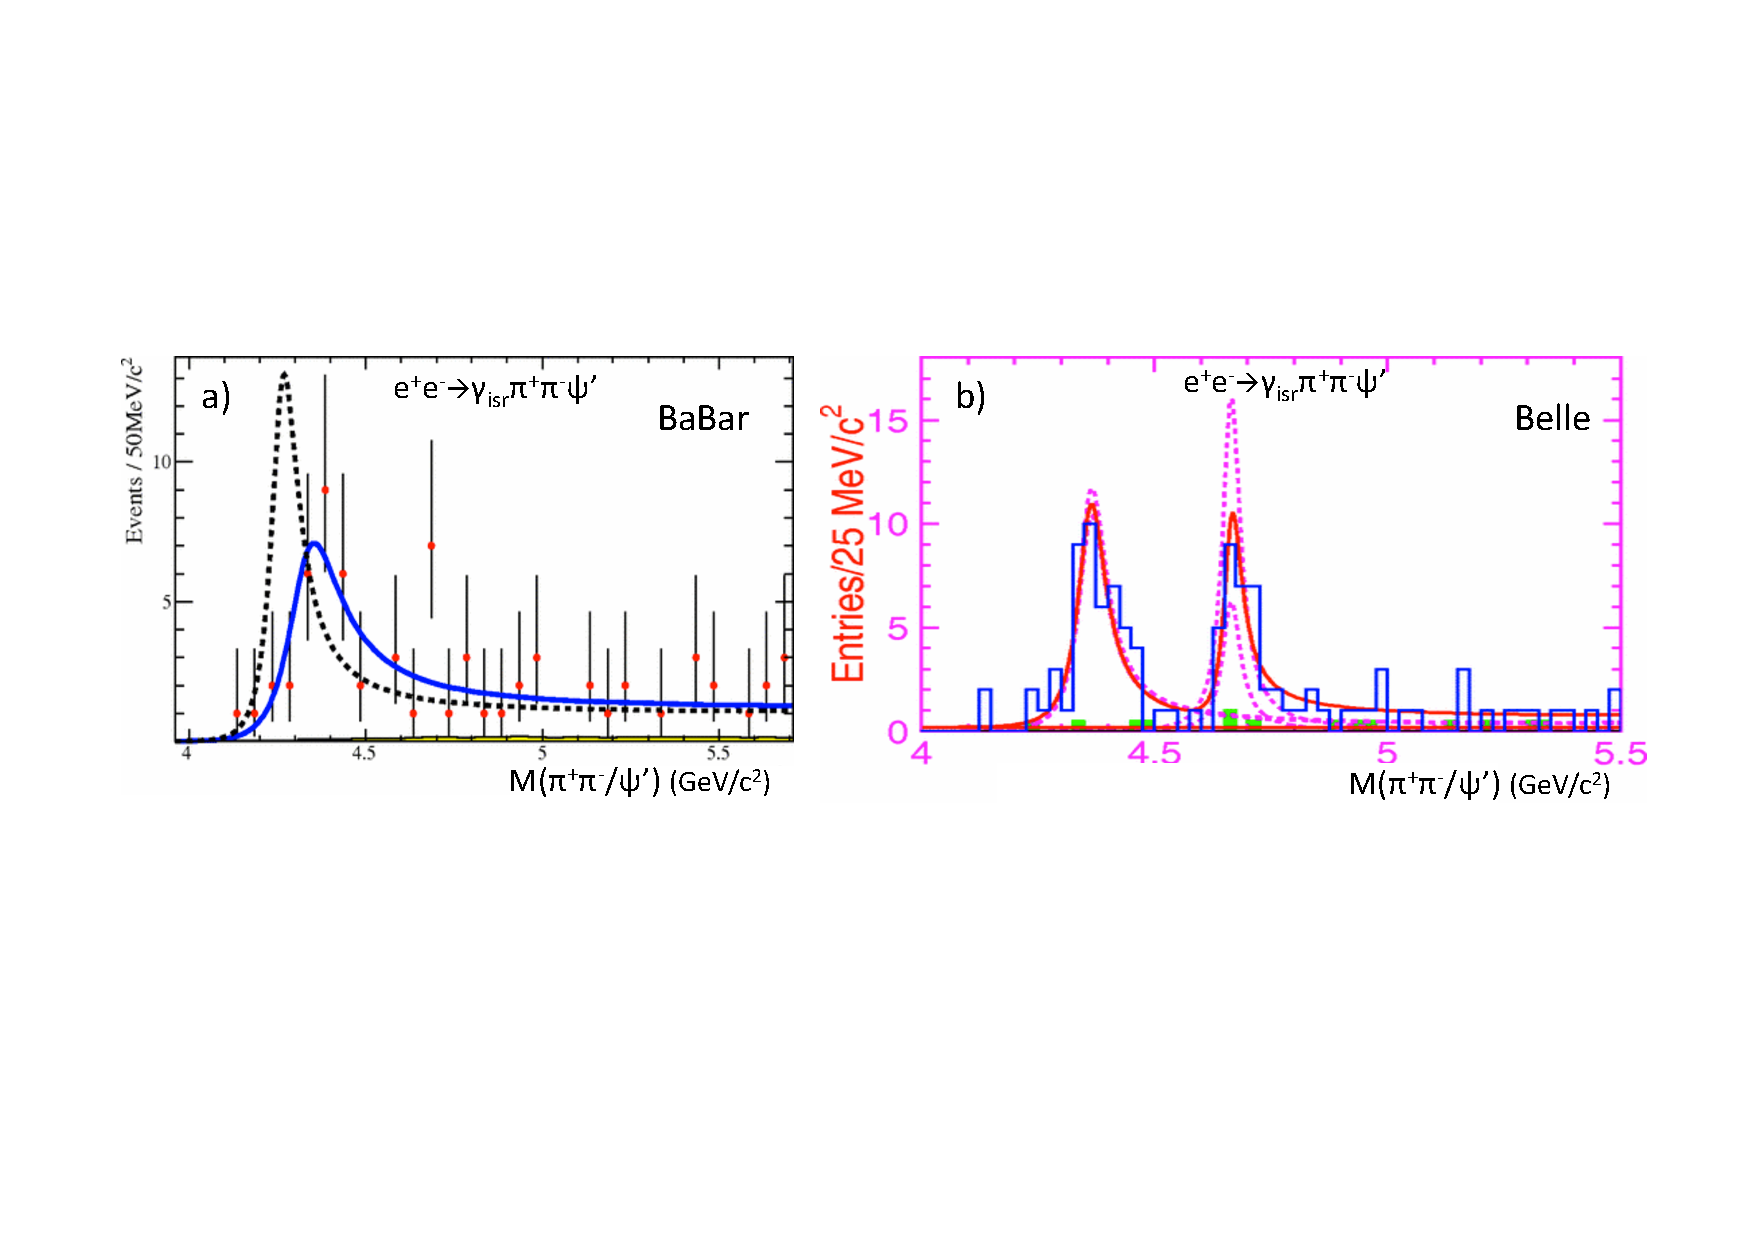
\includegraphics[width=0.9\textwidth]{Figures/01_Introduction/Exotic/neutral_particle/babar-belle_y4360} \\%
   \caption{ The $\jpsi\pip\pim$ invariant mass distribution in the process $\ep\en\to\g\pip\pim\jpsi$ at \babar\supercite{PhysRevD.71.052001}.}
\label{fig:Y4360}
\end{figure}


\begin{figure}[!hbtp]
\centering
   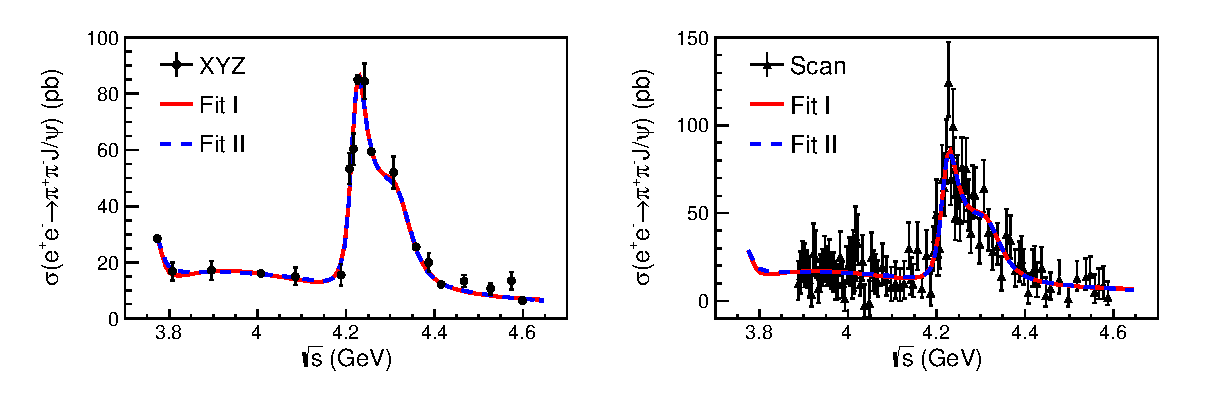
\includegraphics[width=0.9\textwidth]{Figures/01_Introduction/Exotic/neutral_particle/Bes_Y4260} \\%
   \caption{ The cross section for $\ep\en\to\g\pip\pim\jpsi$ at \besiii,
   right one for "high luminosity" scan, 
   left one is "low luminosity" scan\supercite{PhysRevLett.118.092001}.}
\label{fig:bes_Y4260}
\end{figure}


The $J^{PC}$ of $Y$ states is $1^{--}$,
which is as same as photon and \jpsi.
This is a strong evidence that it contains $\cquark\cquarkbar$ quark pair.
However,
all of the $1^{--}$ $\cquark\cquarkbar$ charmonium with mass below 4450 \mev have been seen in the $\ep\en$ collision between 2.6 and 4.6 \gev.   
In addition,
there is no evidence it decaying to open-charmed mesons.
Besed on above considerations,
many theorists infer that this state is multiquark meson or $\cquark\cquarkbar$-gluon hybrid\supercite{PhysRevD.89.114010,PhysRevD.89.116005}. 


The narrow $X(6900)$ was observed by \lhcb in the \jpsi-pair mass spectrum recently\supercite{PAPER-2020-011},
which is the first four charm quarks candidate.  























	
\subsection{Charged multiquark candidates $Z_{c}$ and $Z_{cs}$}

\subsubsection{$Z_{c}$ in $B$ decay }

The first candidate of charged charmonium-like state is $Z(4430)$,
which was observed at \belle in $\Bbar\to\psi\pip\Km$ decay in 2007\supercite{PhysRevLett.110.252001},
and in this plotthe signal structure is shown in the left of Figure.~\ref{fig:Z4430}.
Then the existence of $Z(4430)$ was independently confirmed in 2014 at \lhcb experiment\supercite{LHCb-PAPER-2014-014},
which was studied based on a 4-dimentional amplitude analysis in the $\Bbar\to\psi\pip\Km$ decay.
According to these independent measurements,
the average mass and width are determined to be $M=4478^{+15}_{-81} \mev$ and $\Gamma=181\pm31 \mev$ for $Z_{c}(4430)$.
Besides,
the $J^{P}$ assignment is ascertained to be $1^{+}$ at $9.7\sigma$ level as well.
The corresponding "Argand" plot is shown in the left of Figure.~\ref{fig:Z4430_argand},
revealing the character of Breit-Wigner resonances as a nearly circular in shape.
In addition,
a broad peak named as $Z_{c}(4240)$ is required for a satisfied fitting,
and this additional structure appeared in $\psi\pip$ mass distribution as shown in right of Figure.~\ref{fig:Z4430}.

\begin{figure}[!hbtp]
\centering
   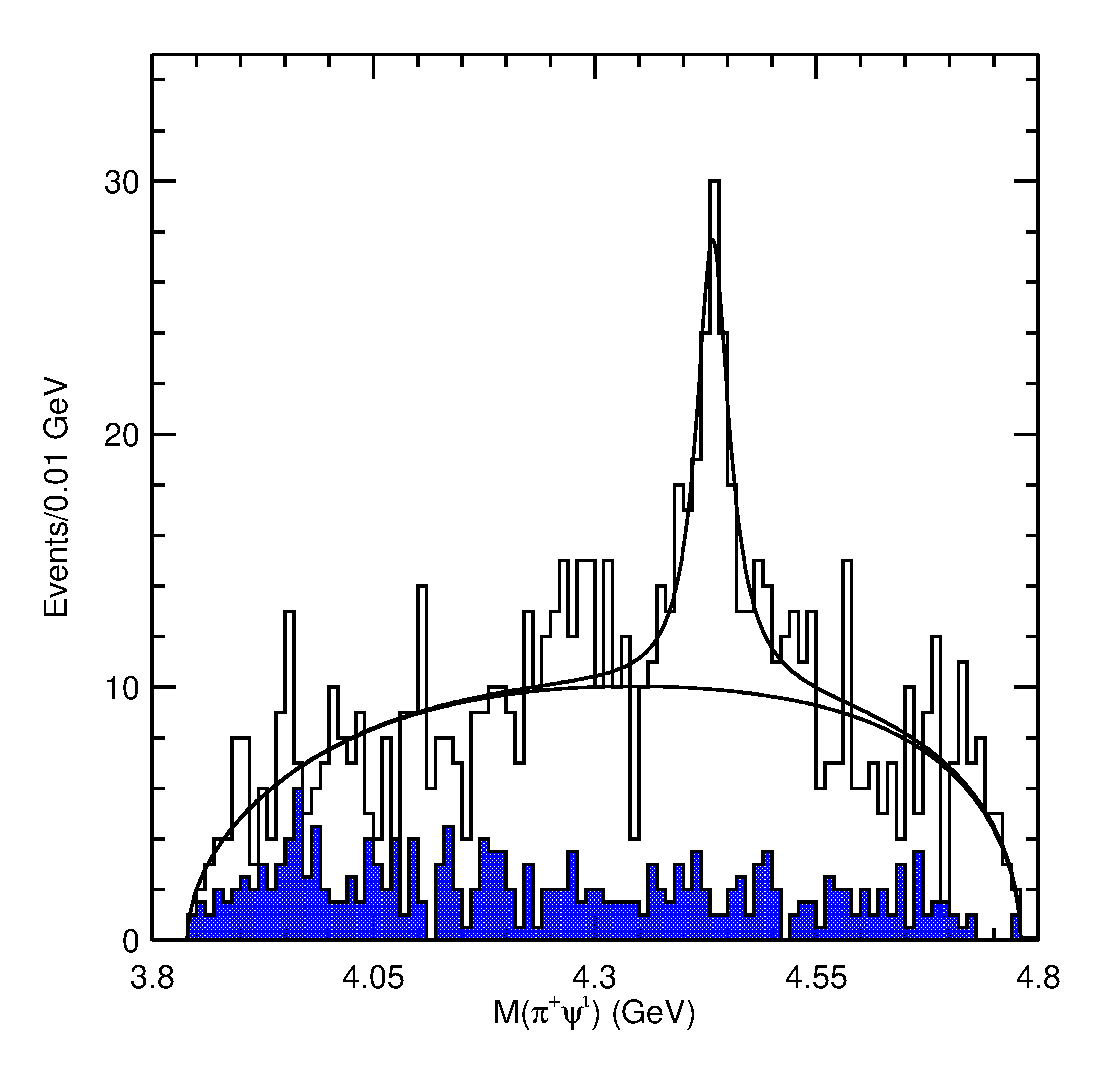
\includegraphics[width=0.43\textwidth]{Figures/01_Introduction/Exotic/charged_particle/Belle_Z4430} %
   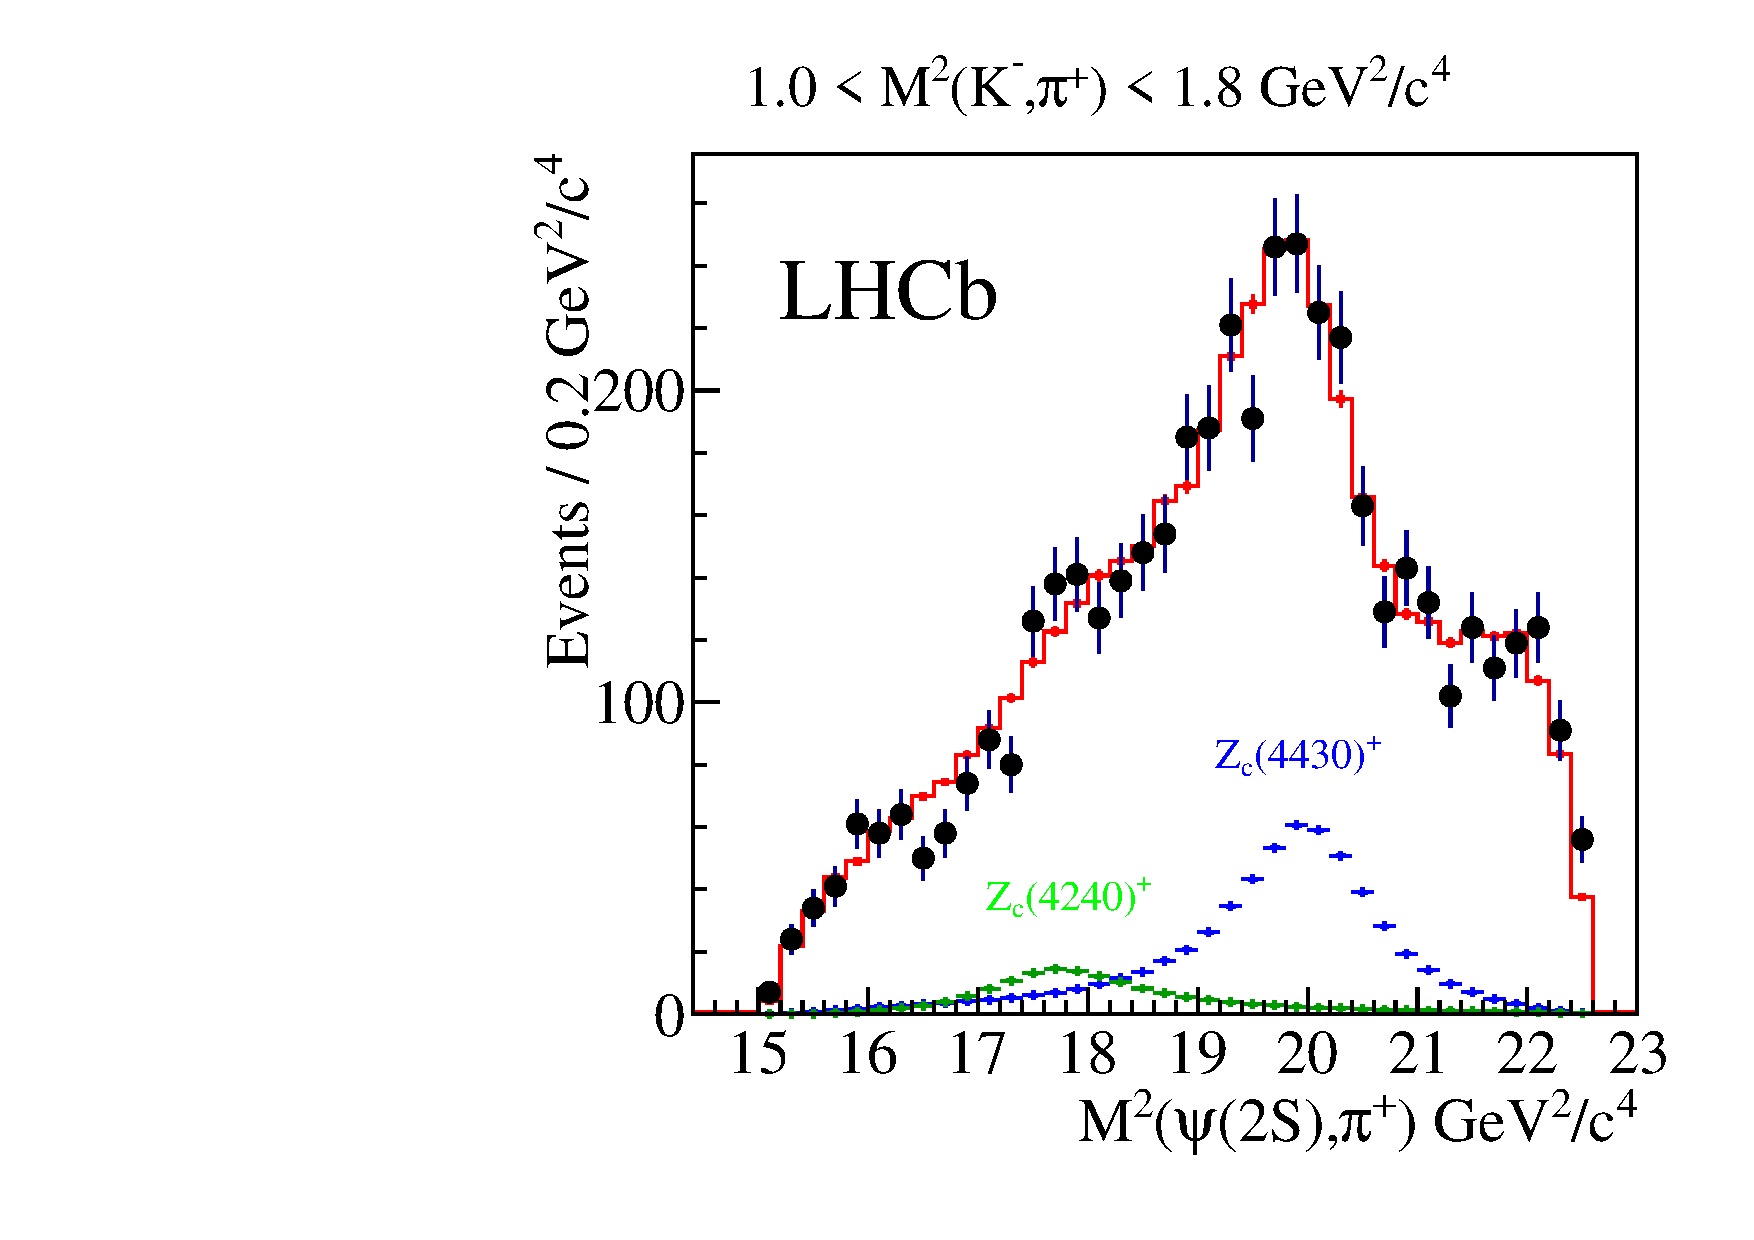
\includegraphics[width=0.46\textwidth]{Figures/01_Introduction/Exotic/charged_particle/LHCb_Z4430} %
   \caption{ 
   The $M(\psi\pi)$ distribution in $\Bbar\to\psi\pip\Km$ decay at \belle\supercite{PhysRevLett.110.252001},  
   the $M^{2}(\psi\pi)$ in $\Bbar\to\psi\pip\Km$ from \lhcb\supercite{LHCb-PAPER-2014-014}.}
\label{fig:Z4430}
\end{figure}


\begin{figure}[!hbtp]
\centering
   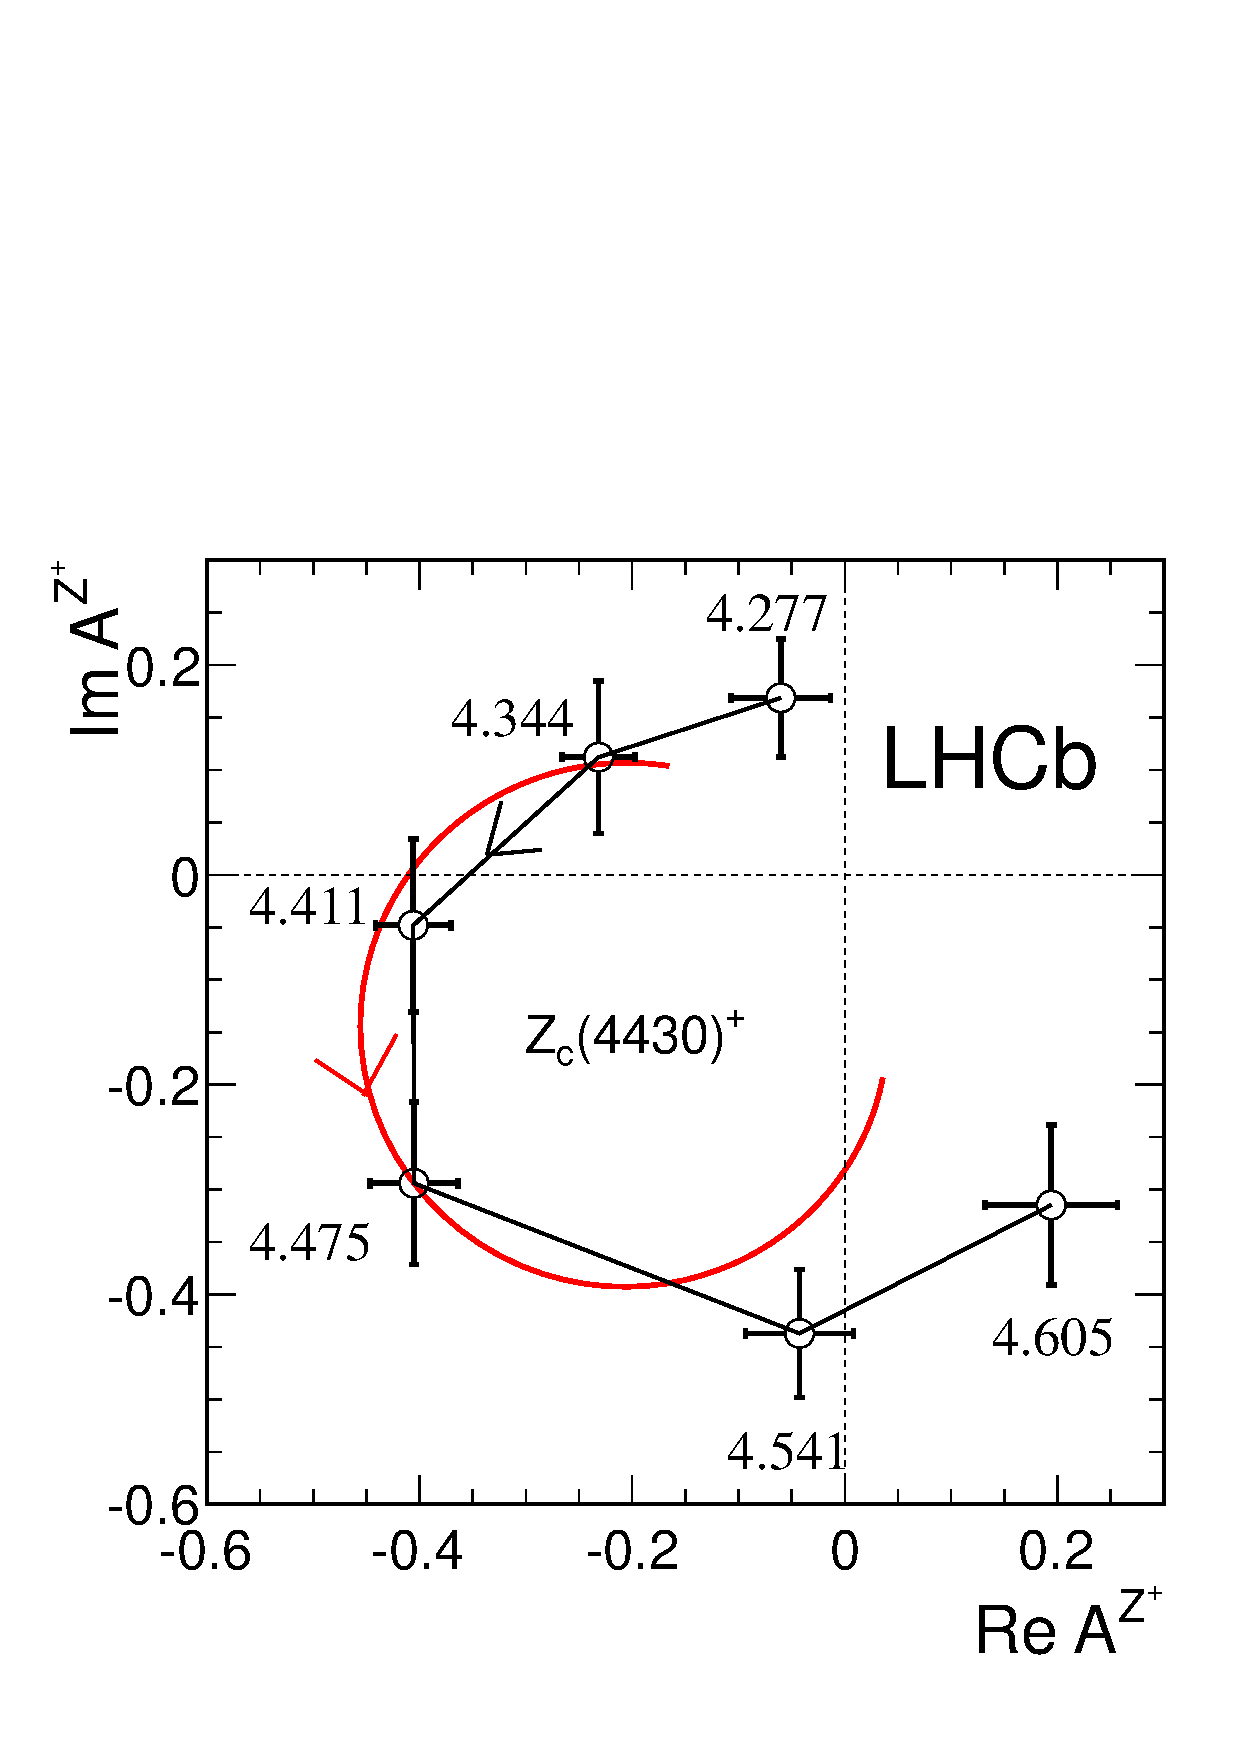
\includegraphics[width=0.4\textwidth]{Figures/01_Introduction/Exotic/charged_particle/Argand-Z} %
   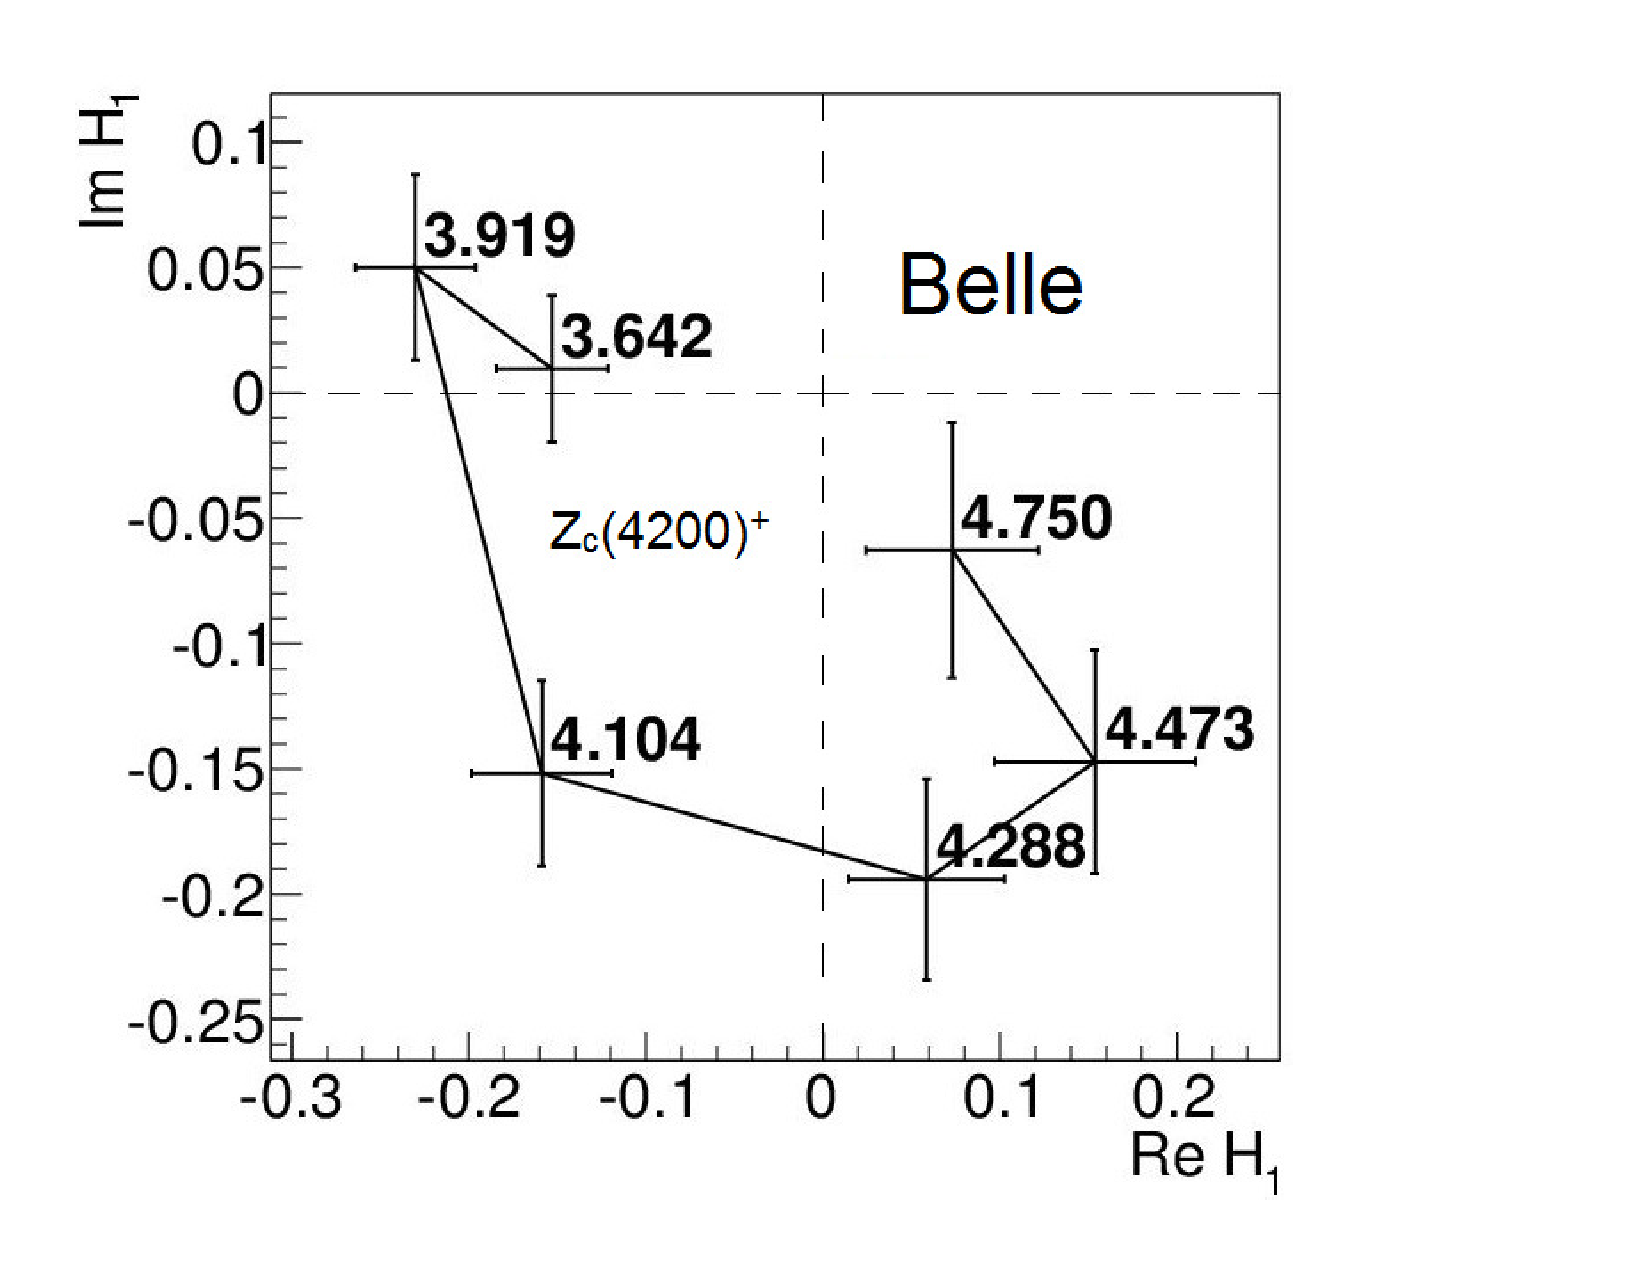
\includegraphics[width=0.52\textwidth]{Figures/01_Introduction/Exotic/charged_particle/Belle-Zc4200-Argand} %
   \caption{ 
   The real and imaginary parts of the amplitude for $Z_{c}(4430)\to\psi\pip$ decay at \lhcb\supercite{LHCb-PAPER-2014-014},  
   the $Z_{c}(4200)\to\jpsi\pip$ decay from \belle\supercite{PhysRevD.90.112009}.}
\label{fig:Z4430_argand}
\end{figure}

\belle also performed an amplitude of $\Bbar\to\jpsi\pip\Km$ decays\supercite{PhysRevD.90.112009},
and a new very broad $1^{+}$ $Z_{c}(4200)$ state is required for a satisfactory fit.
The measured mass and width of this state are $M=4196^{+31}_{-29}\pm^{+17}_{-13} \mev$ and $\Gamma=370\pm70^{+70}_{-132} \mev$.
Besides,
\belle also reported corresponding $J^{P}$ is either $0^{-}$ or $1^{+}$,
and "Argand" plot is shown in the right of Figure.~\ref{fig:Z4430_argand},
which displays a nearly circular phase motion.

The charged $Z_{c}$ states are pretty broad,
and the interference effect is very obvious, 
which can distort the resonance line shape.
For example,
the original $Z_{c}(4430)$ results were based on a one dimentional Breit-Wigner line-shape fit,
so they obtained lower values of mass and width than that from \lhcb.


\subsubsection{$Z_{c}$ in $\ep\en$ collision}

As mentioned in Section.~\ref{subsub:Y4260},
the $Y(4260)$ was observed at \babar.
This discovery prompted \besiii group to collect data at $E_{cm}=4260 \mev$ to search possible charged resonance 
in this channel.
%was excluded by \besiii.
Then,
the $Z_{c}(3900)$ was observed in $\jpsi\pip$ and $\jpsi\pim$ invariant mass distribution, 
using a 525 $\rm{pb^{-1}}$ \besiii data sample accumulatd at $E_{cm}=4.26\gev$\supercite{PhysRevLett.110.252001},
as shown in the left of Figure.~\ref{fig:3900}.
The measured mass is $3899.0\pm6.1 \mev$ and the width is $46\pm22$.
Significantly,
the mass of this state is around $24 \mev$ above the $m_{\Dstarp}+m_{\Dstarzb}$ threshold.
The $Z_{c}(3900)$ was observed by Belle at about the same time\supercite{PhysRevLett.110.252002}.

\begin{figure}[!hbtp]
\centering
   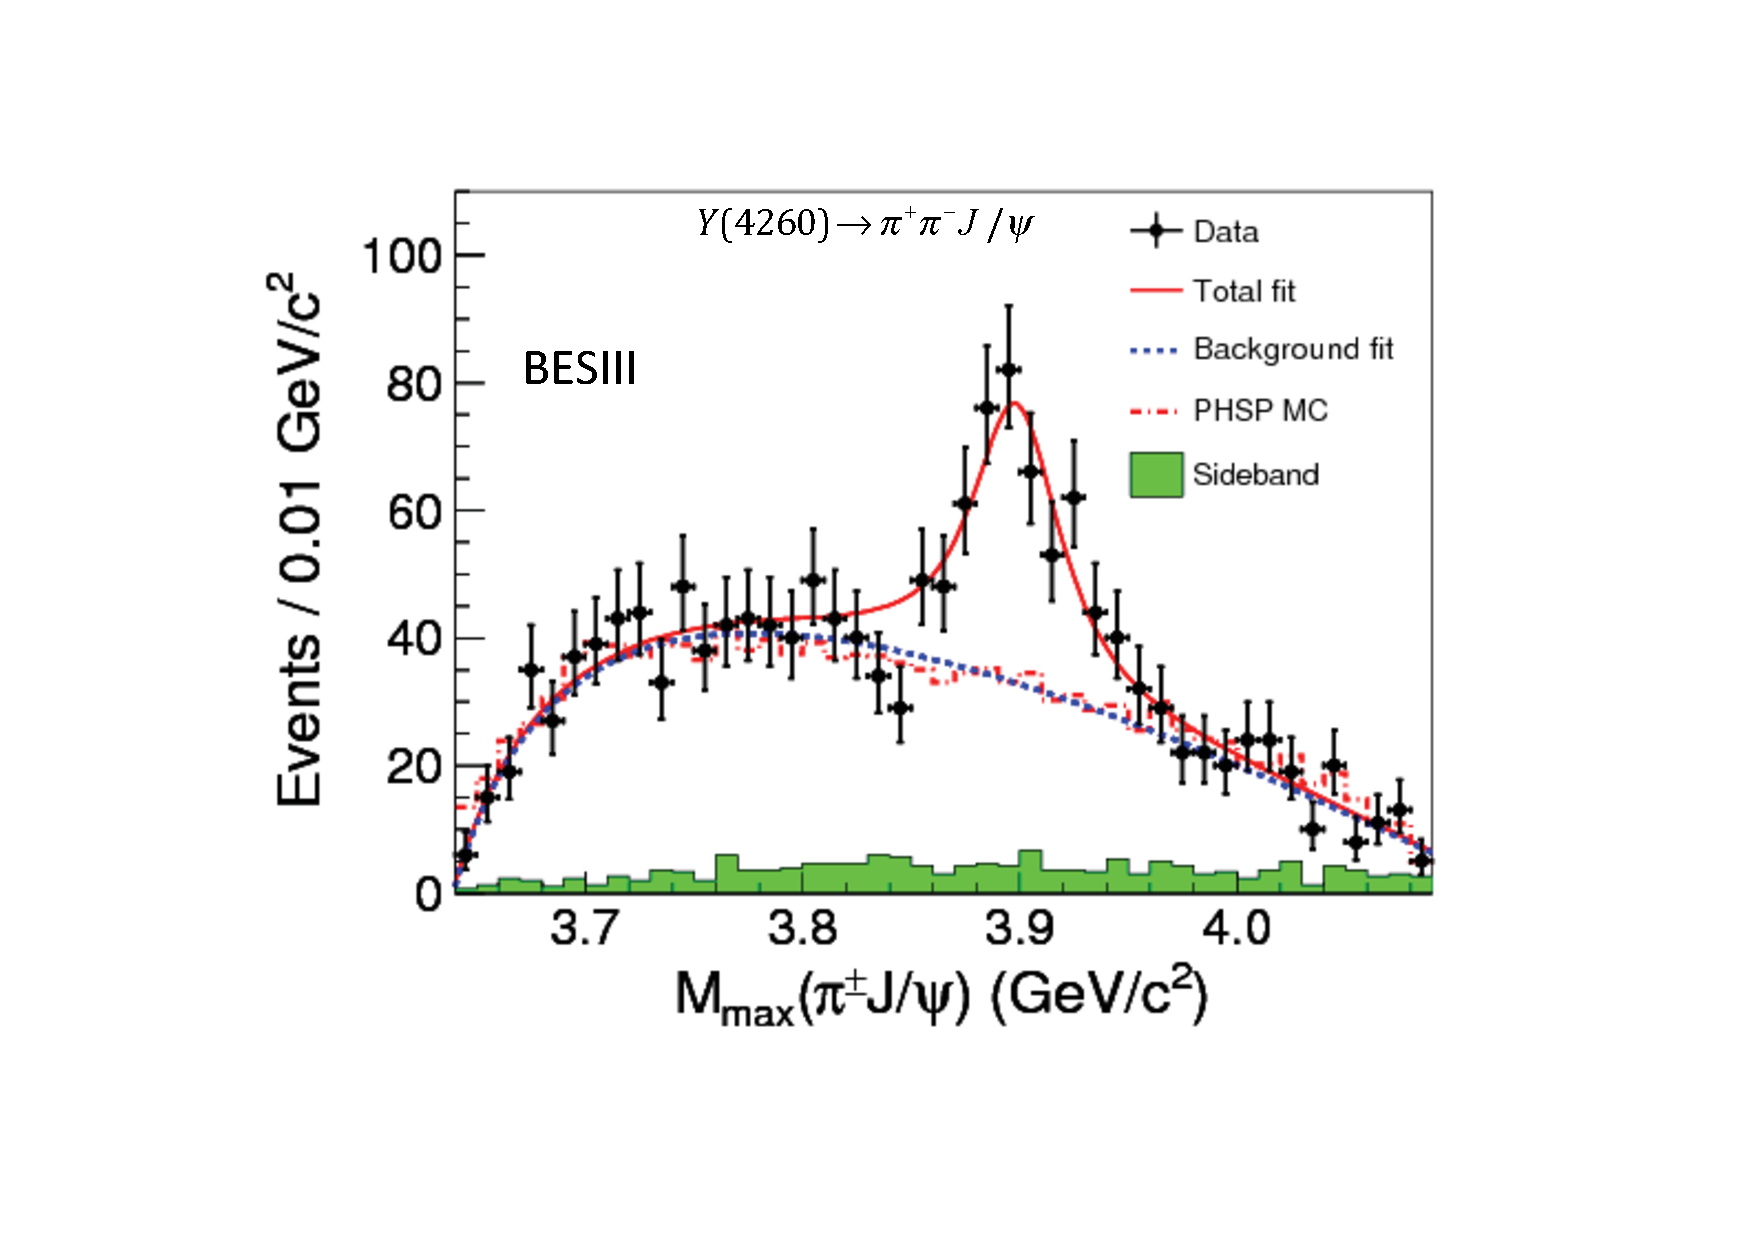
\includegraphics[width=0.43\textwidth]{Figures/01_Introduction/Exotic/charged_particle/bes3_zc3900} %
   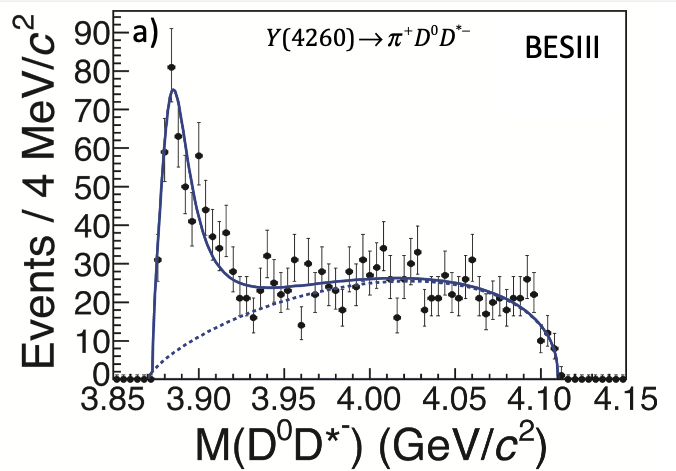
\includegraphics[width=0.46\textwidth]{Figures/01_Introduction/Exotic/charged_particle/bes3_Z3900_DD} %
   \caption{ 
   Distribution of the larger of two $\jpsi\pi^{\pm}$ masses in $\ep\en\to\jpsi\pip\pim$ events collected in \besiii
   at $E_{cm}=4260 \mev$\supercite{PhysRevLett.110.252001} (left),
   The $\Dz\Dstarm$ invariant mass distribution in $\ep\en\to\Dz\Dstarm\pip$ events collected in \besiii at $E_{cm}=4260 \mev$
   \supercite{PhysRevLett.112.022001} (right)}.
\label{fig:3900}
\end{figure}

Subsequently,
\besiii explored the $\Dz\Dstarm$ invariant mass distribution in $\ep\en\to\Dz\Dstarm\pip$ events,
and found the very strong near-threshold peak in this distribution,
as shown in the right of Figure.~\ref{fig:3900}.
Then the mass and width are determined as $M=3883.9\pm4.5 \mev$ and $\Gamma=24.8\pm12 \mev$ from a one-dimentional fit,
where the peak was discribed by a threshold-modified BW amplitude 
and background was repesented by a incoherent phase-space-like function\supercite{PhysRevLett.112.022001}.
Thus, 
this state was named as $Z_{c}(2885)$ by \besiii collaboration.
From the $Z_{c}(2885)\to\D\Dstarb$ stong decay,
\besiii also determined the $J^{P}$ quantum number to be $1^{+}$,
which is prefered than the $0^{-}$ or $1^{-}$ assignments.
\besiii also reported the observation of isospin partner of $Z_c(3900)$ in $\ep\en\to\jpsi\piz\piz$ events\supercite{PhysRevLett.115.112003},
as well as in $\ep\en\to\Dp\Dstarm\piz$\supercite{PhysRevLett.112.022001},
with mass and width are consistent with the charged $Z_{c}(3900)$ state.


In addition to $Z_c(3900)$,
\besiii collaboration observed the $Z_c(4020)$ in $h_c(1P)\pip\pim$ final states\supercite{PhysRevLett.111.242001},
and the invariant mass distribution of $h_{s}\pi^{\pm}$ is shown in the left of Figure.~\ref{fig:Z4020}.
In this study,
the mass of $Z_c(4020)$ was measured to be $4022.9\pm2.8 \mev$,
which is about $5 \mev$ above $m_{\Dstarp}+m_{\Dstarzb}$.
Similar to the neutral $Z_c(3900)$ study,
the isospin partner of $Z_c(4020)$ was searched in $\ep\en\to h_{c}\piz\piz$ events\supercite{PhysRevLett.113.212002},
as shown in the right of Figure.~\ref{fig:Z4020}.
Afterwards,
$Z_c(4020)$ and its isospin partner were searched in $\ep\en\to\Dstarp\Dstarz\pim$\supercite{PhysRevLett.112.132001} 
and $\ep\en\to\Dstar\Dstarzb\piz$\supercite{PhysRevLett.115.182002} events by \besiii. 
The measured mass and width from the double \D invariant mass spectrum are agree with those measured 
for the $Z_c(4020)\to h_{c}\pip$ channel within errors.

\begin{figure}[!hbtp]
\centering
   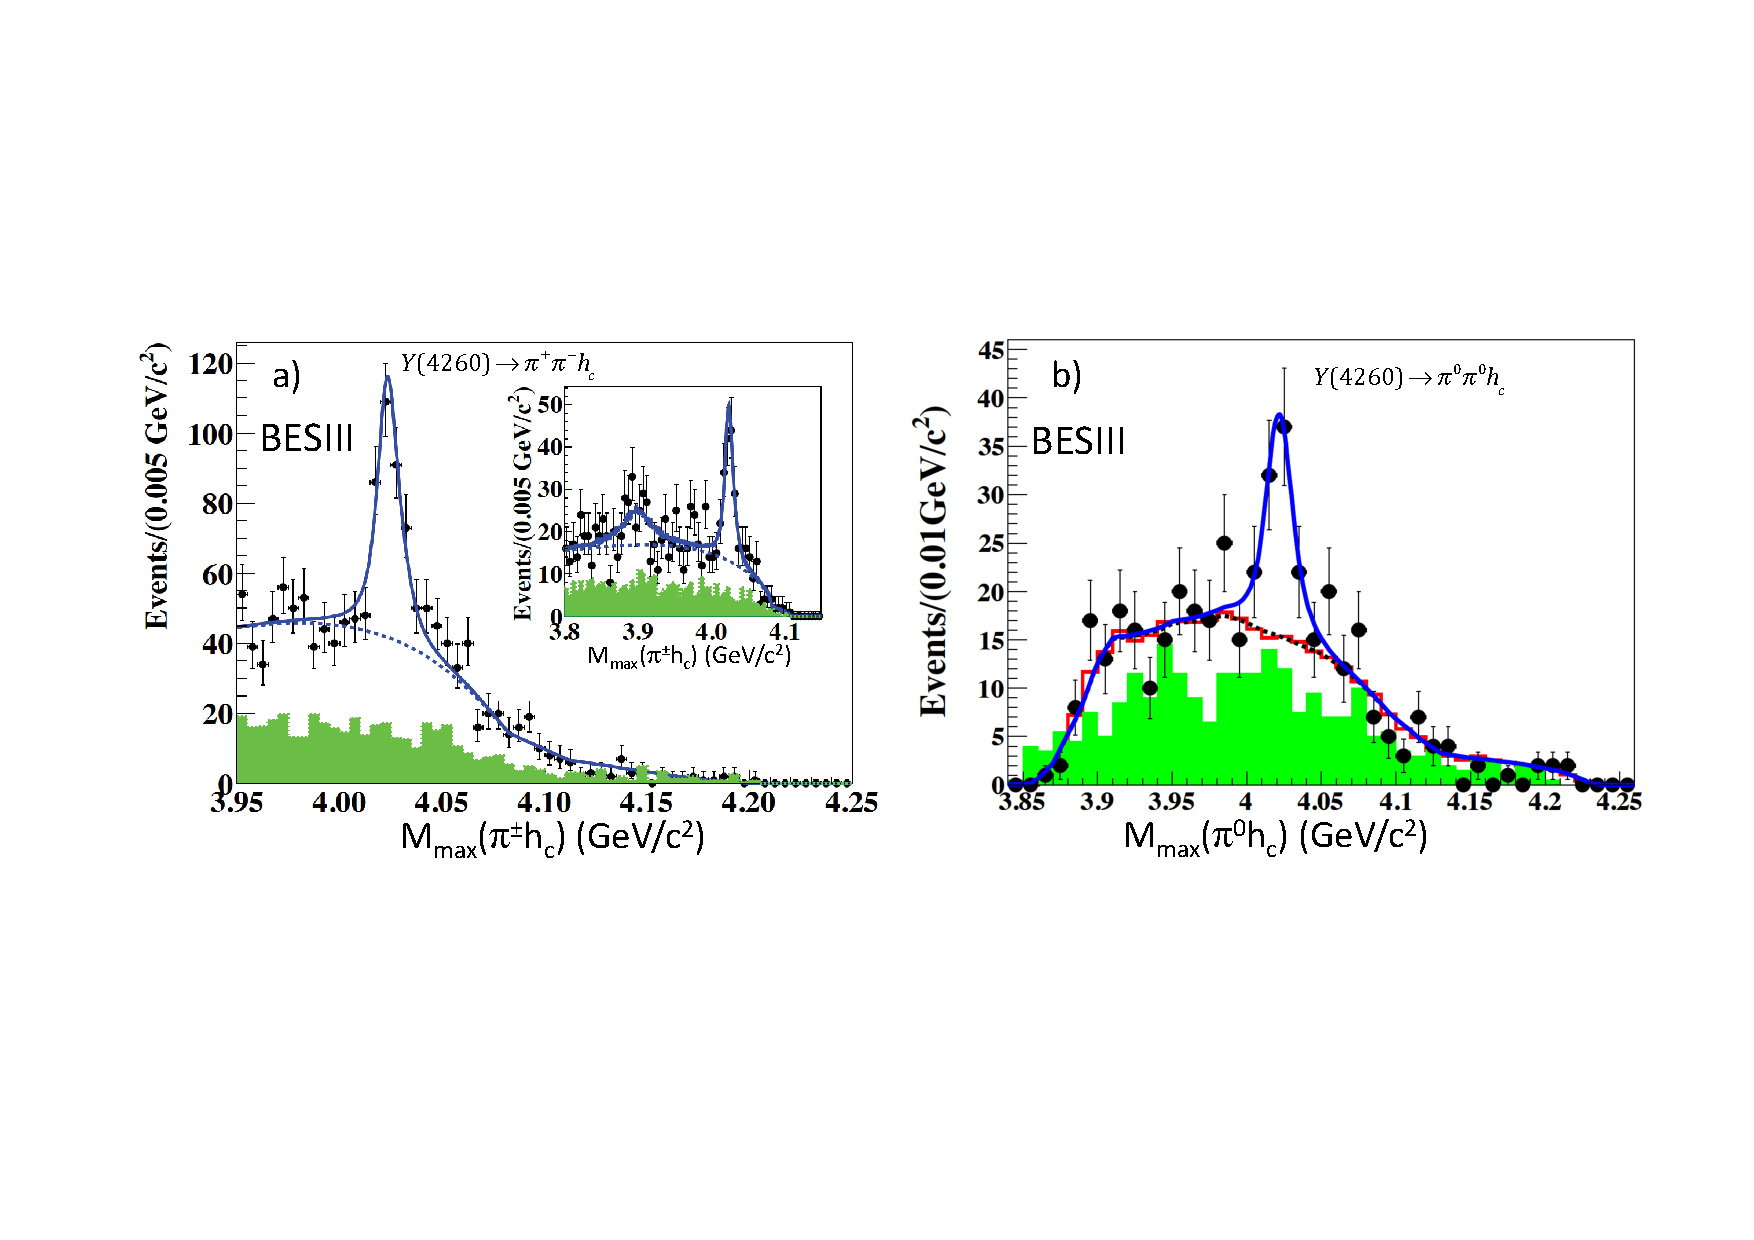
\includegraphics[width=0.95\textwidth]{Figures/01_Introduction/Exotic/charged_particle/bes3_zc4020_pihc} %
   \caption{ 
   Distribution of the larger of two $h_{c}\pi^{\pm}$ masses in $\ep\en\to h_{c}\pip\pim$ events collected in \besiii
   at $E_{cm}=4260 \mev$ and $E_{cm}=4360 \mev$\supercite{PhysRevLett.111.242001} (left),
   The $h_{c}\piz$ invariant mass distribution in $\ep\en\to h_{c}\piz\piz$ events collected in \besiii at \besiii
   \supercite{PhysRevLett.113.212002} (right)}.
\label{fig:Z4020}
\end{figure}

The theoretical pictures of $Z_c(3900)$ and $Z_c(4020)$ are not very clear yet.
For example,
the mass of these two states are in agreement with the molecular interpretation,
and both $Z_c$ states should copiously decay to $h_{c}\pi$ in a purely molecular interpretation.
But the $Z_c(4020)$ is not observed in $\jpsi\pi$
and $Z_c(3900)$ is not observed in $h_{c}\pi$.




\subsubsection{Observation of $Z_{cs}$ states}
\label{subsubsec:01_Zcs_observation}


Recently,
the \besiii experiment reported observation of the threshold structure in the $D_s^-\Dstarz+\Dssm\Dz$ mass distribution~\supercite{Ablikim:2020hsk}. 
This structure is interpreted as a resonance, 
and is named as $Z_{cs}(3985)^-$. 
The measured mass of this resonance is $3982.5_{-2.6}^{+1.8}\stat\pm2.1\syst$\mev and width is equal to $12.8_{-4.4}^{+5.3}\stat\pm3.0\syst$\mev,
and the significance of this state is around $5.3\sigma$.
The corresponding \Kp recoil-mass distributions are shown in Figure.~\ref{fig:Zcs3985},

\begin{figure}[!hbtp]
\centering
   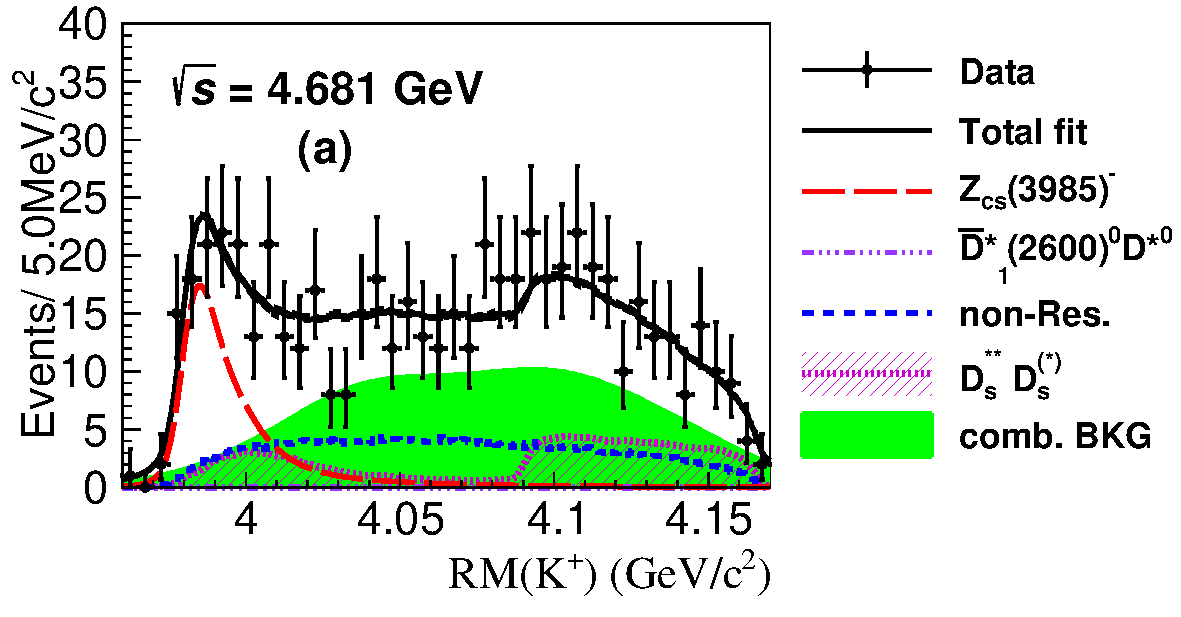
\includegraphics[width=0.51\textwidth]{Figures/01_Introduction/Exotic/Zcs/data_4680_Simulfit_withsig-eps-converted-to} %
   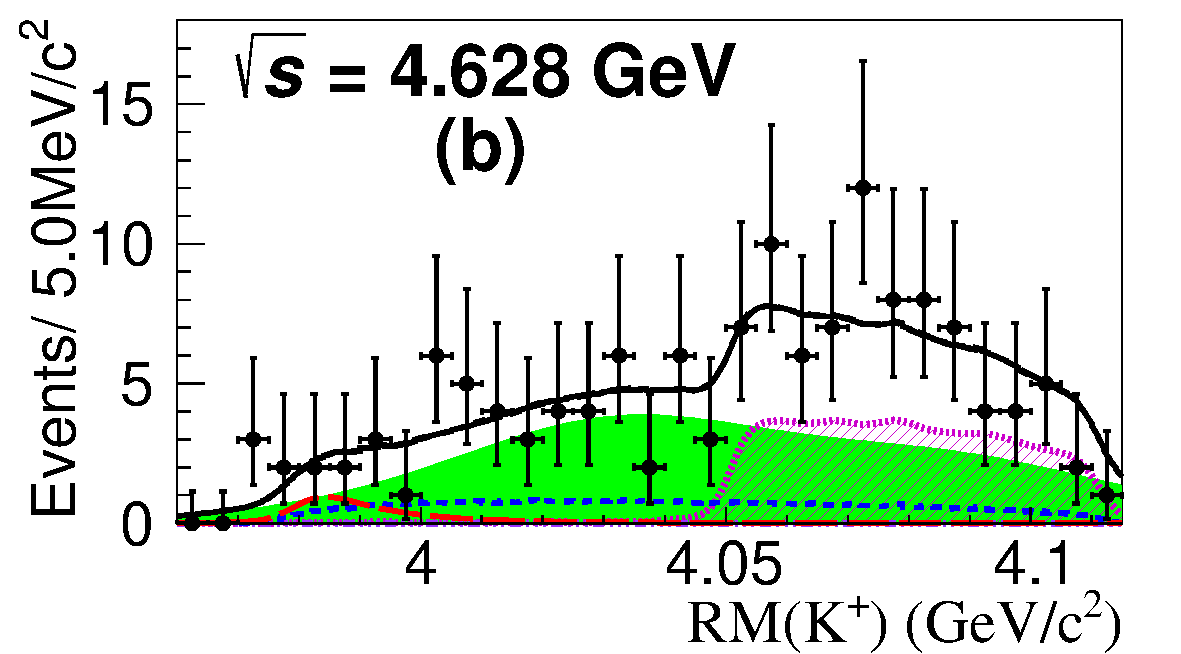
\includegraphics[width=0.48\textwidth]{Figures/01_Introduction/Exotic/Zcs/data_4626_Simulfit_withsig-eps-converted-to} %
   \caption{ 
   Simultaneous unbinned maximum likelihood fit to the \Kp recoil-mass spectra in data at 4.681 \gev (left) and 4.628 \gev (right)
   \supercite{Ablikim:2020hsk}.}
\label{fig:Zcs3985}
\end{figure}

Before the results from \besiii were reported, 
we had observed two $Z_{cs}$ states,
as well as several new $X$ states,
in $\Bp\to\jpsi\phi\Kp$ decay based on a 6-dememtional amplitude analysis at \lhcb.
The detailed analysis procedure is introduced in Chapter.~\ref{chap:Zcs_study},
and some main conclusions are illustrated here.
Figure~\ref{fig:Zcs4000_dalitz} shows the Dalitz plots for \Bp candidates in the signal region.
The most apparent features are four bands in the $\jpsi\phi$ mass distribution, 
corresponding to the previously reported $X(4140)$, $X(4274)$, $X(4500)$ and $X(4700)$ states.
There is also a distinct $\jpsi\Kp$ band near $16\gev^2$,
which is the sign of $Z_{cs}(4000)$.

\begin{figure}[!hbtp]
\centering
   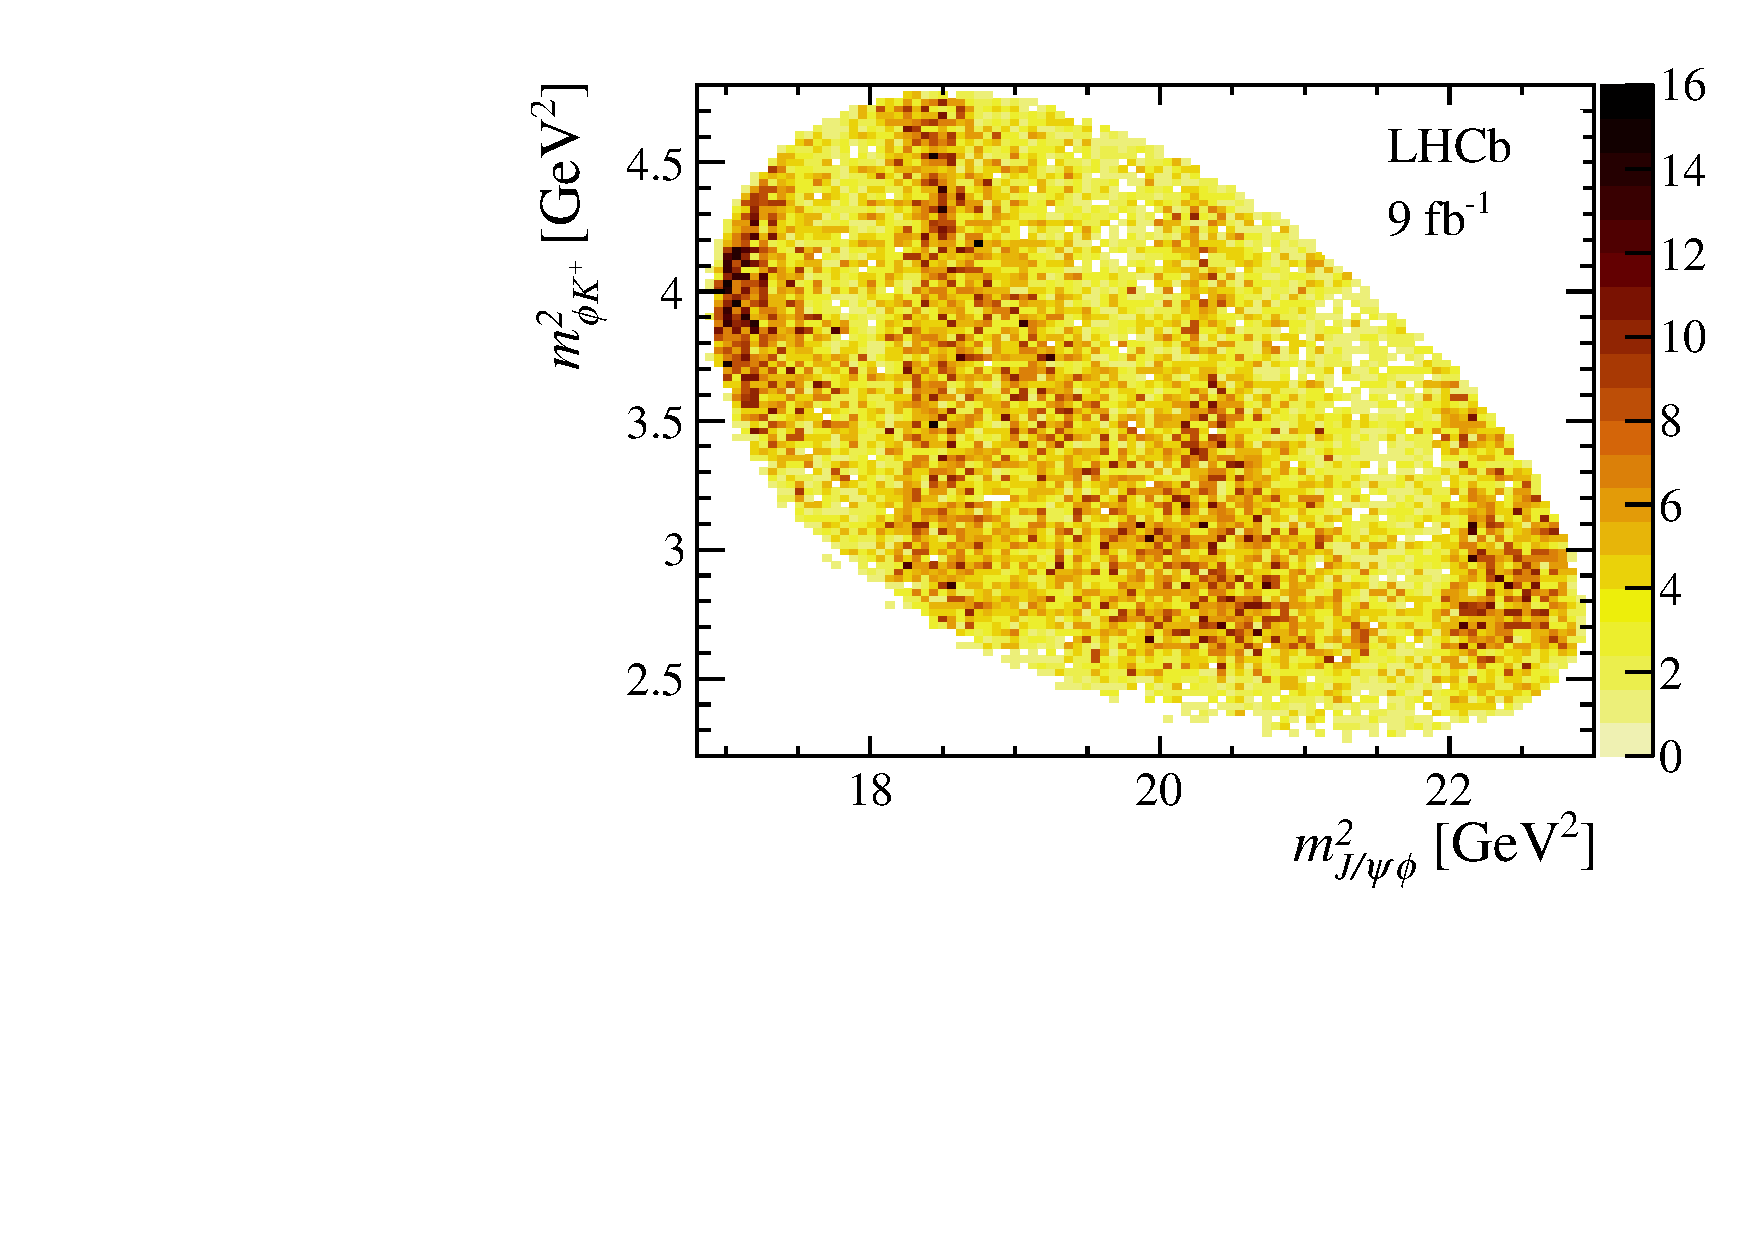
\includegraphics[width=0.45\textwidth]{Figures/01_Introduction/Exotic/Zcs/mphik2_mjpsiphi2} %
   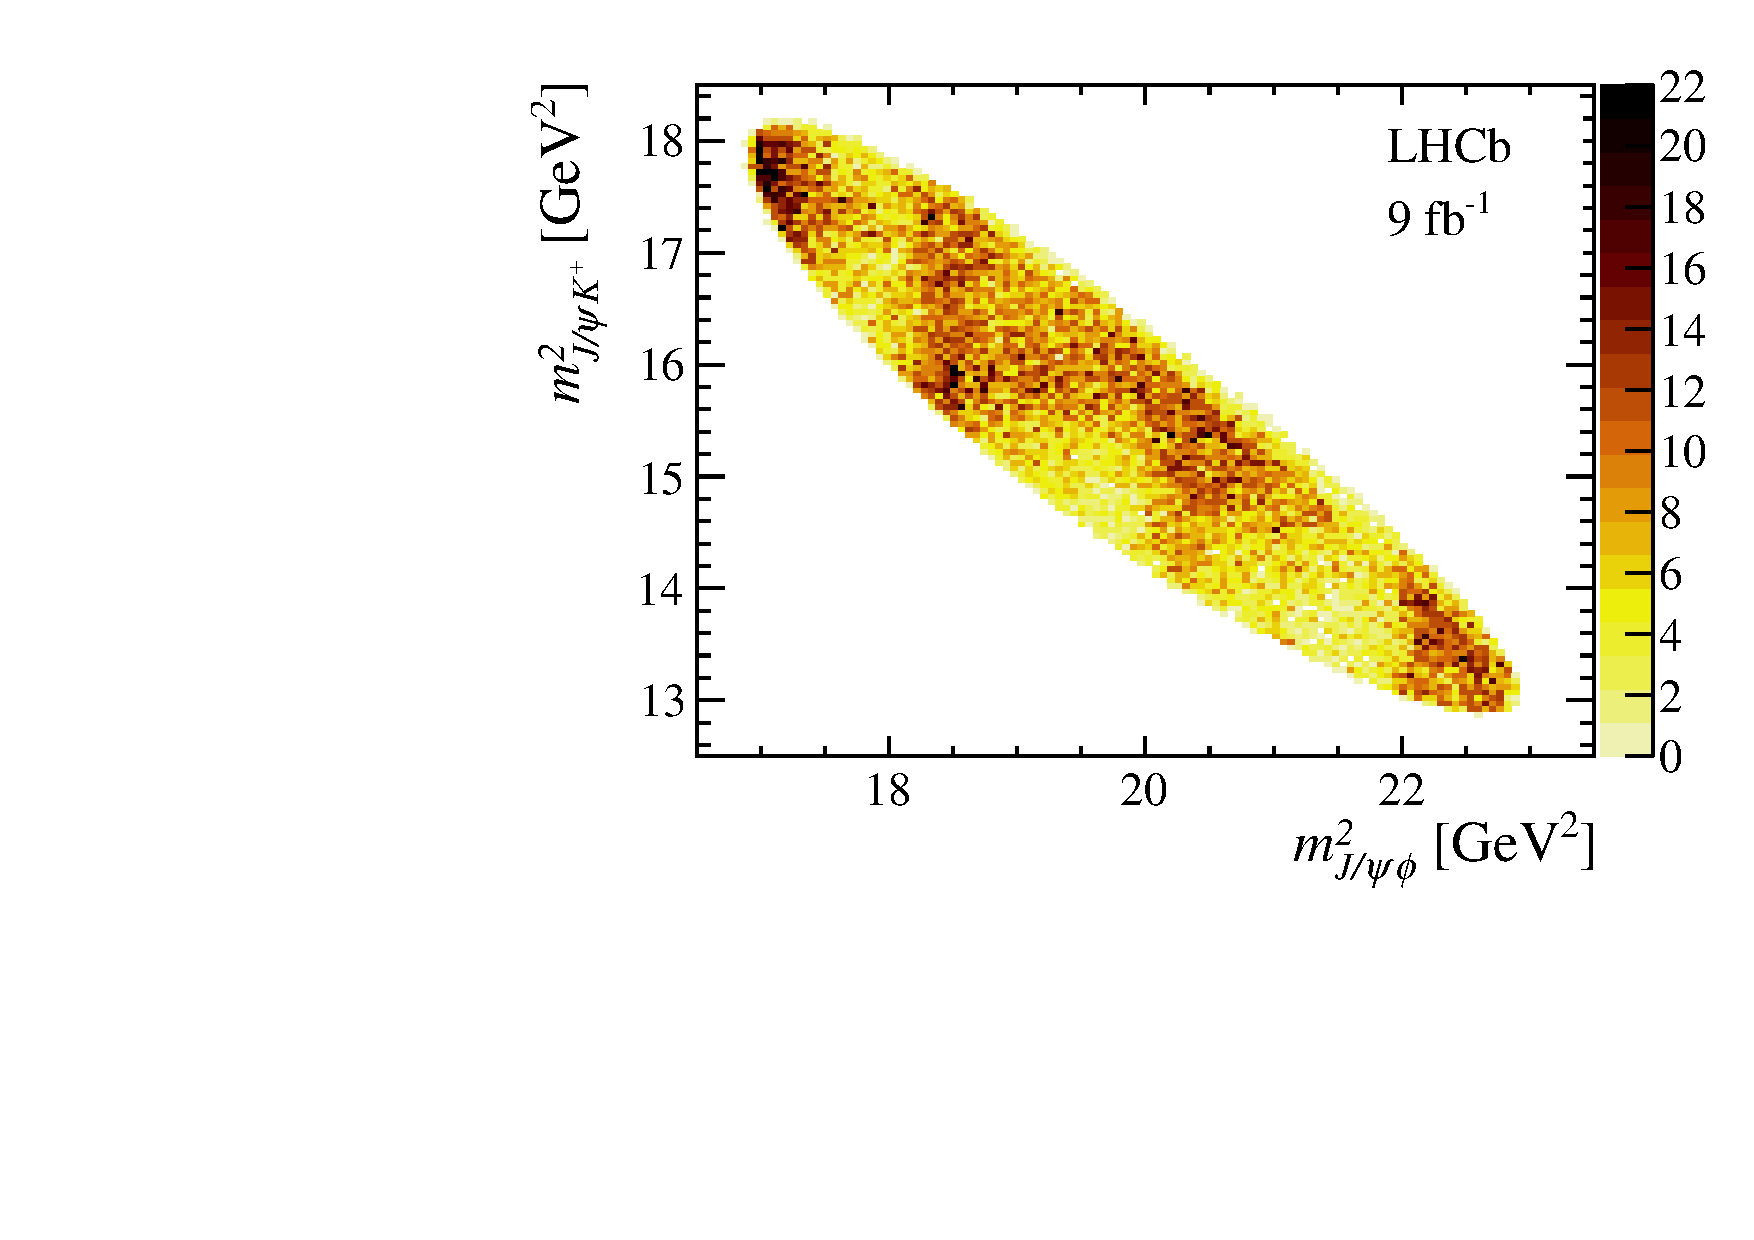
\includegraphics[width=0.45\textwidth]{Figures/01_Introduction/Exotic/Zcs/mjpsik2_mjpsiphi2} %
   \caption{ 
   Dalitz plots for $\Bu\to\jpsi\phi\Kp$ candidates in a region $\pm$15\mev around the $B^+$ mass peak.}
\label{fig:Zcs4000_dalitz}
\end{figure}

The left two plots in Figure~\ref{fig:Zcs4000} shows the $m_{\jpsi\Kp}$ distributions in two slices of $m_{\jpsi\phi}$,
which illustrates the need for the narrower $Z_{cs}(4000)^+$ state. 
Beside,
the spin and parity of $Z_{cs}(4000)$ is determined to be $1^{+}$. 
Further evidence for the resonant character of $Z_{cs}(4000)^+$ is observed in the right plot of Figure.~\ref{fig:Zcs4000}, 
showing the evolution of the complex amplitude on the Argand diagram.
The magnitude and phase exhibit approximately circular evolution with $m_{\jpsi\Kp}$ in the counter-clockwise direction,
as expected for a resonance.

We consider the $Z_{cs}(4000)$ observed at \lhcb and $Z_{cs}(3985)$ claimed by \besiii are not same state.
First, 
the width of these two states are pretty different.
Second,
we tried to fix the mass of width of $Zcs(3985)$ in $\Bp\to\jpsi\phi\Kp$ amplitude model,
but no significant likelihood improvement was obtained by this procedure. 
Considering the similar $Z_{c}(3900)$ and $Z_{c}(4020)$ have not been observed at any $B$ meson decay channel,
the production mechanism for $Z_{cs}(4000)$ and $Z_{cs}(3985)$ should be different.


\begin{figure}[!hbtp]
\centering
   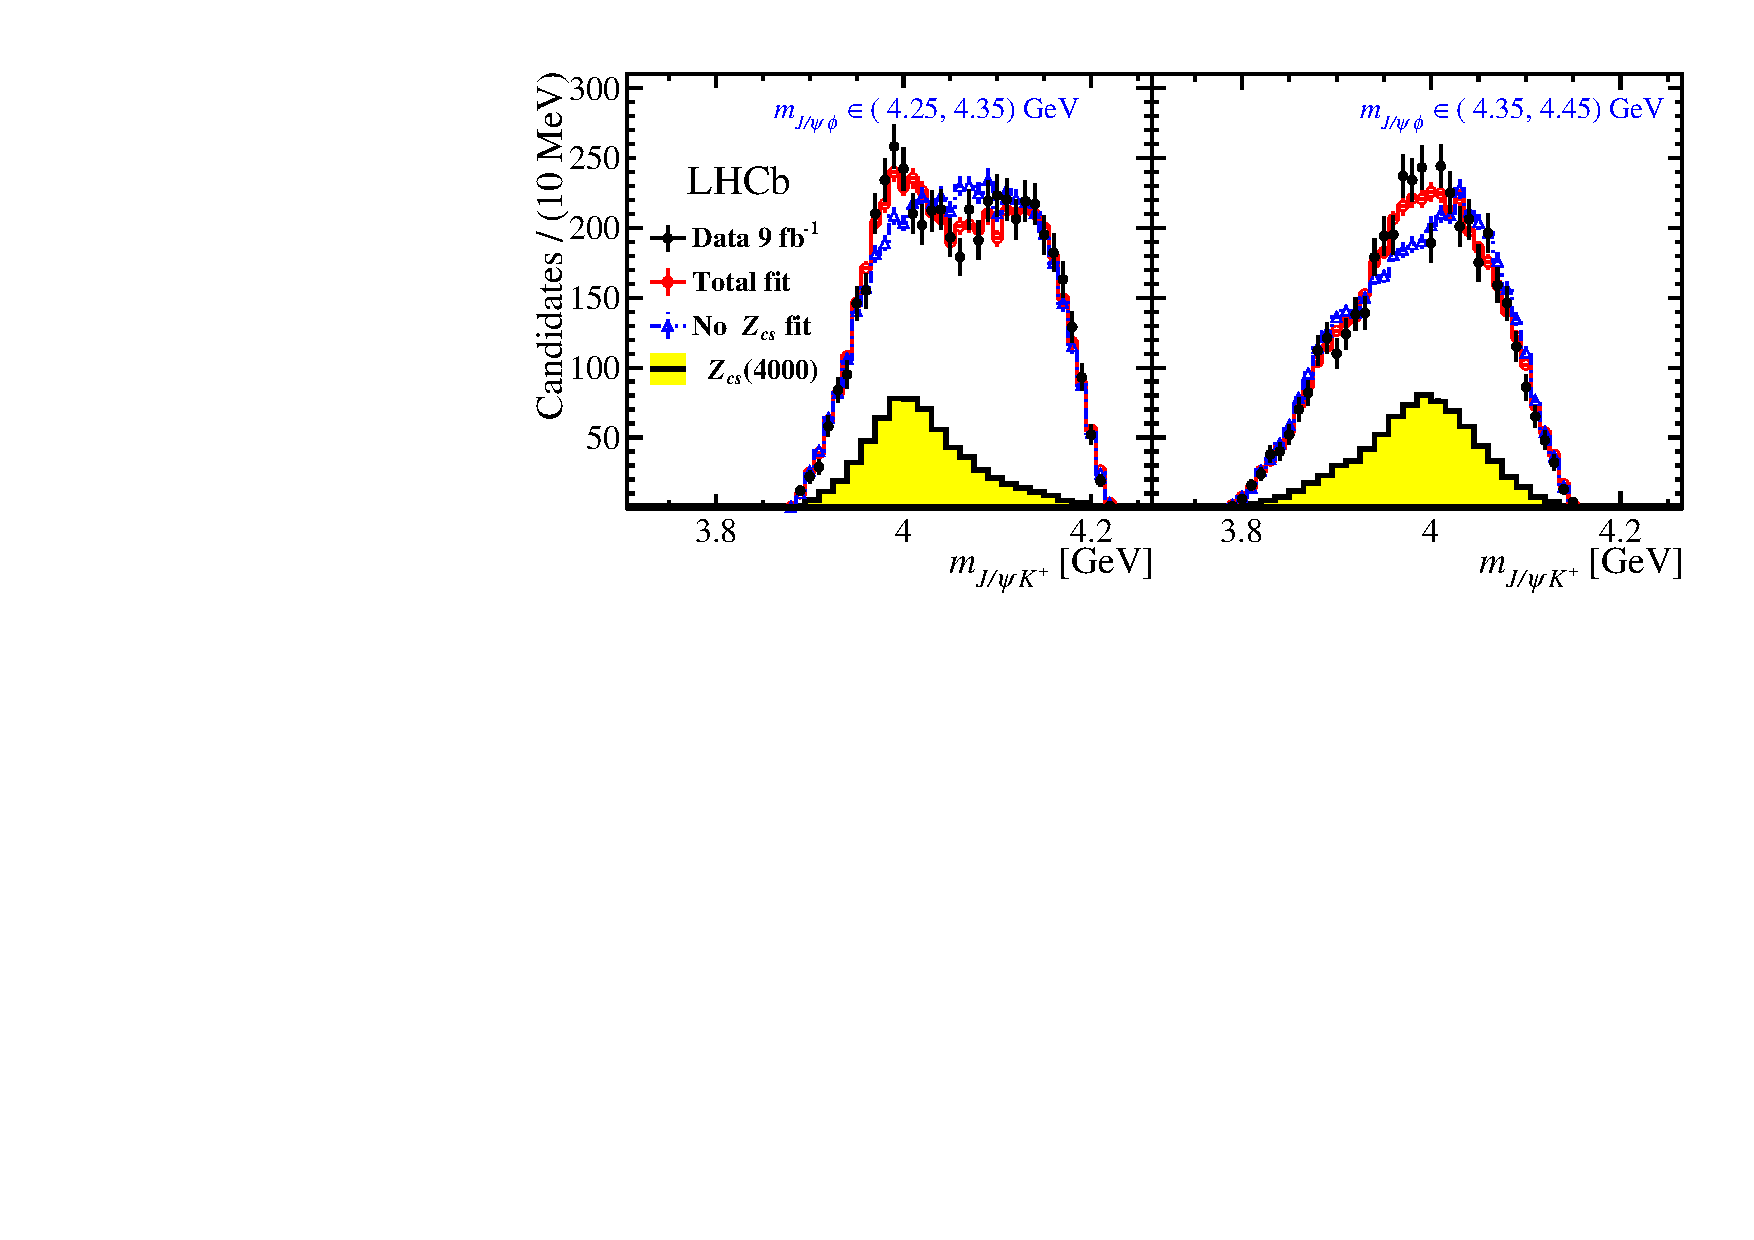
\includegraphics[width=0.65\textwidth]{Figures/01_Introduction/Exotic/Zcs/jpsik_projection} %
   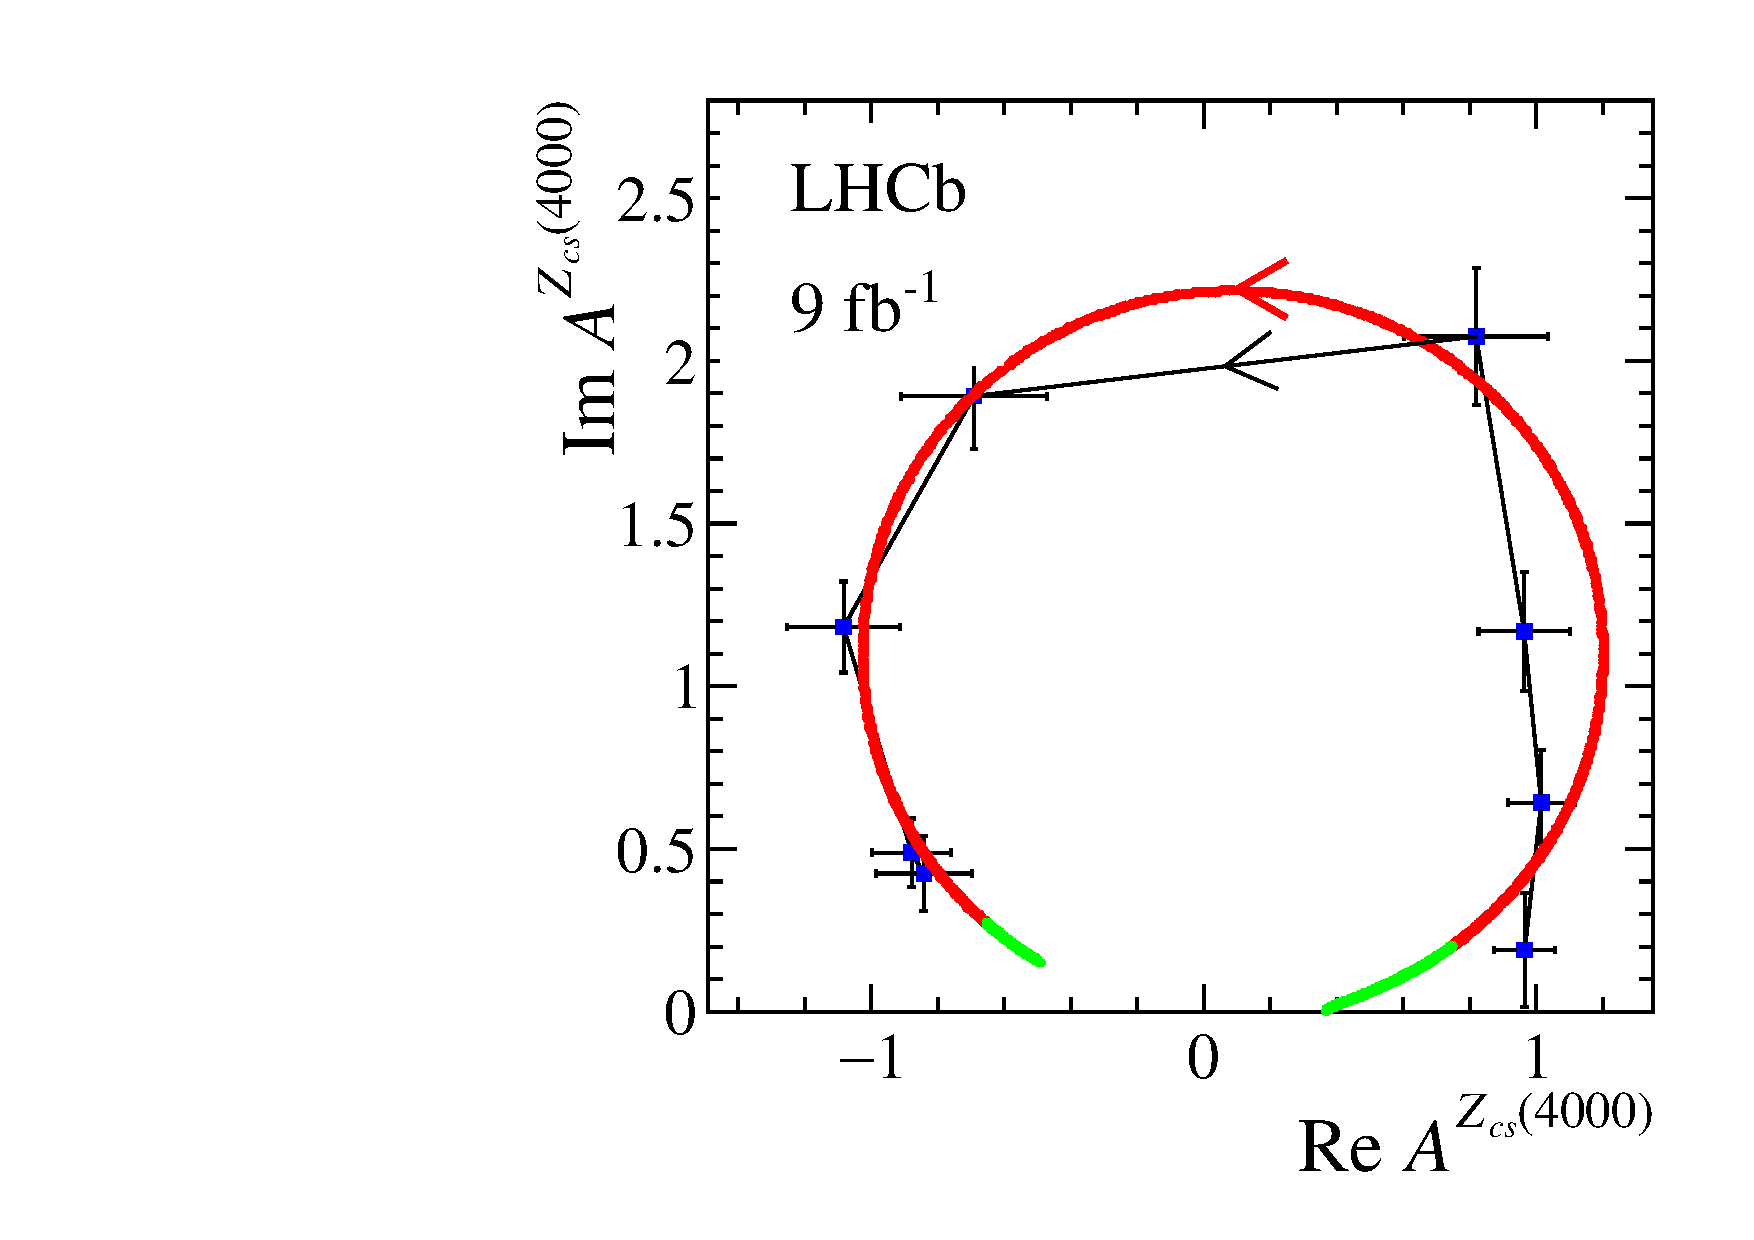
\includegraphics[width=0.325\textwidth]{Figures/01_Introduction/Exotic/Zcs/Z1_argand} %
   %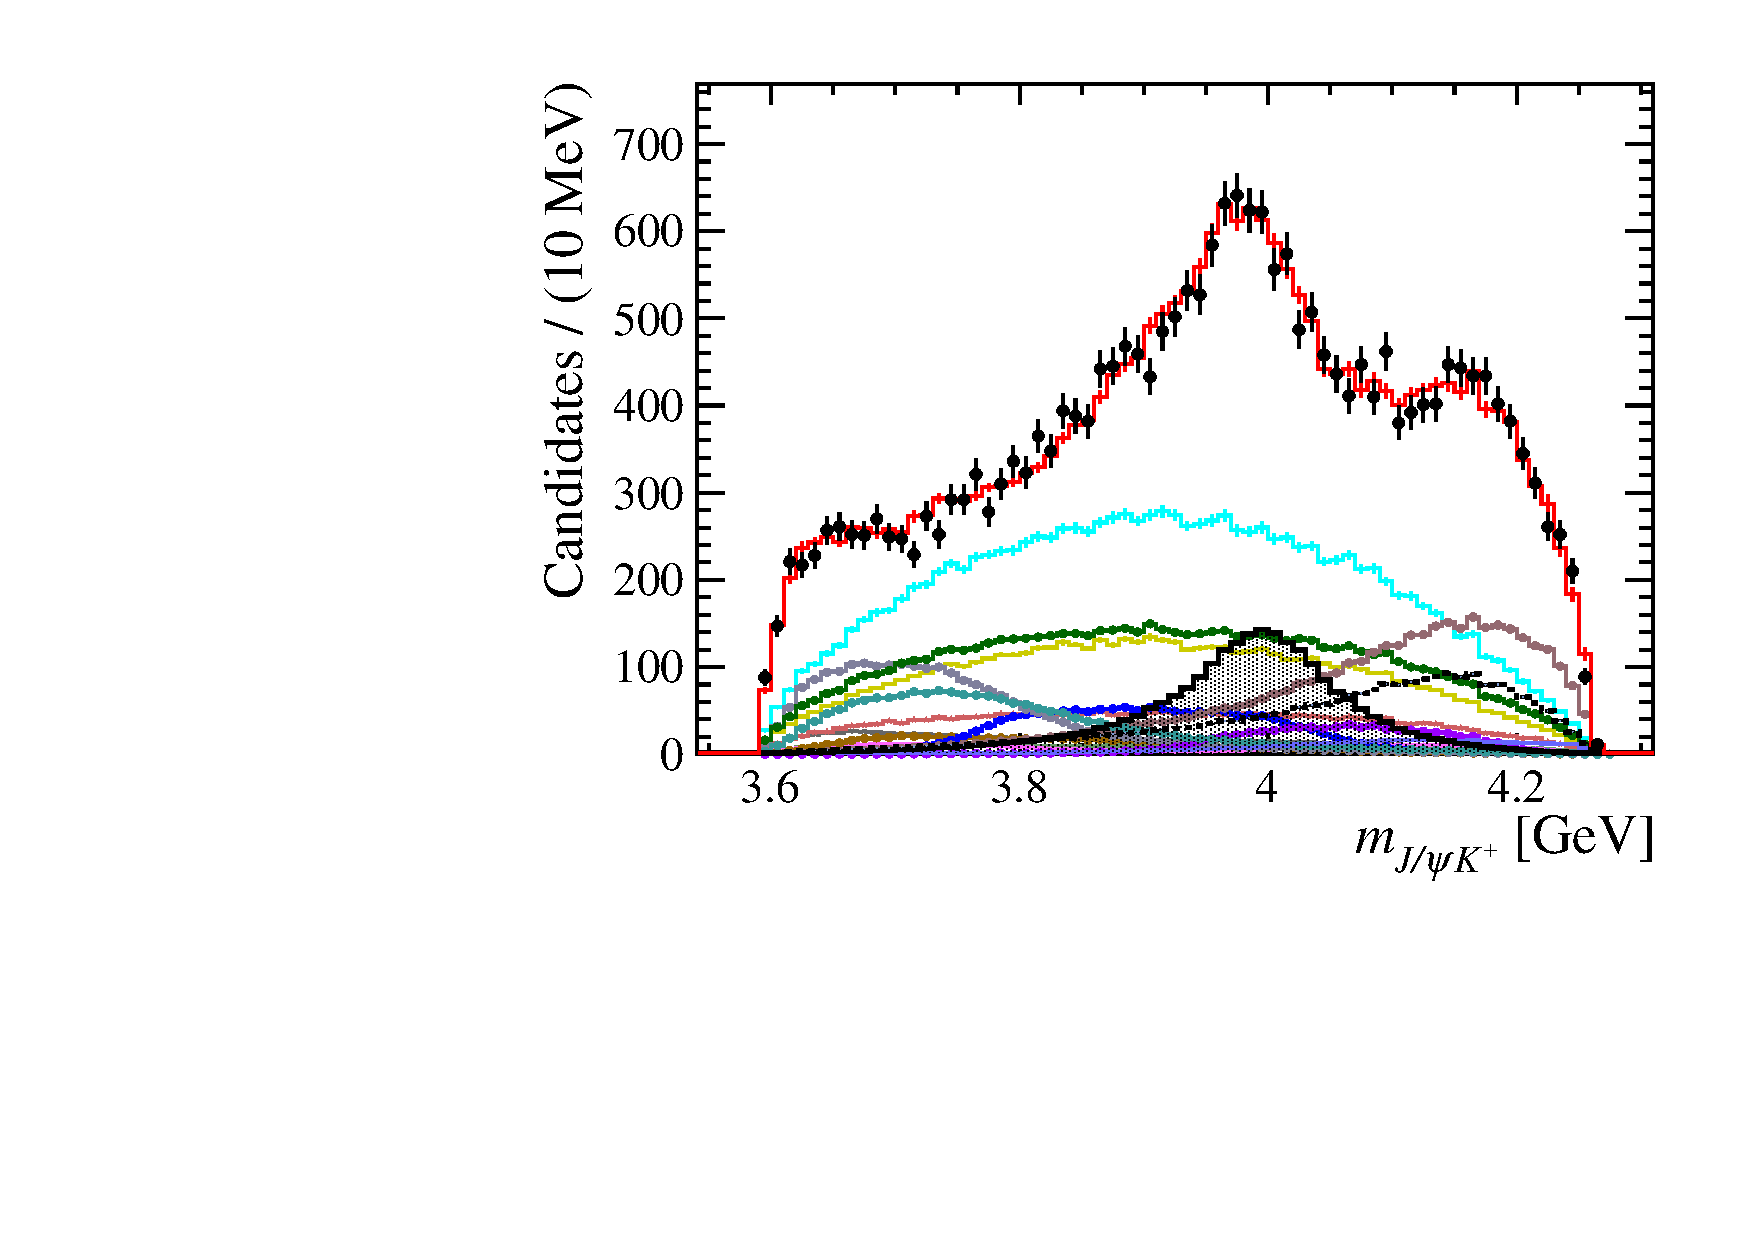
\includegraphics[width=0.4\textwidth]{Figures/01_Introduction/Exotic/Zcs/mjpsik-New} %
   \caption{
   Fit projections onto $m_{\jpsi\Kp}$ in two slices of $m_{\jpsi\phi}$ for the default model and the default model 
   without the $1^+$ $Z_{cs}$ states (left and middle) .
   Fitted values of the $Z_{cs}(4000)^+$ amplitude in eight $m_{\jpsi\Kp}$ bins,
   shown on an Argand diagram (blue points).
   The red curve represents the expected Breit-Wigner behaviour between $-1.4\Gamma_0$ to $1.4\Gamma_0$ around the $Z_{cs}(4000)^+$ mass.
   The green curve is the same as the red curve but the mass is extended to the reachable range in the $\Bp\to\jpsi\phi\Kp$ channel (right).}
\label{fig:Zcs4000}
\end{figure}

The mass thresholds of $\Ds\Dzb$ excitations, 
with S-wave $J^P$ values, 
are shown in Table~\ref{tab:mt1} and \ref{tab:mt2}.
The $Z_{cs}(4000)$ and $Z_{cs}(3985)$ are close to the thresholds 
and the S-wave $J^P$ are consistent to the results obtained from the amplitude fit. 
Higher values of angular momentum are expected to be suppressed for threshold effects.

\begin{table}[h]
\scriptsize
%\scriptsize
\begin{center}
\caption{Mass threshold and S-wave $J^P$ of $\Ds\Dzb$ containing $\ccbar u\squarkbar$.}
\label{tab:mt2}
\begin{tabular}{|c|c|c|c|}
\hline
L=0                   &\tabincell{c}{$0^-$ \Dsp \\ (1968\mev)}
&\tabincell{c}{$1^-$ \Dssp \\ (2112\mev)}             &\tabincell{c}{$0^+$ $D^{*+}_{s0}$ \\ (2318\mev)}        \\
\hline
\tabincell{c}{$0^-$ \Dz \\ (1870\mev)}                &\tabincell{c}{$0^+$ \\ (3838\mev)}
&{\color{red} \tabincell{c}{ $1^+$ \\ (3982\mev)} }   &\tabincell{c}{$0^-$  \\ (4188\mev)}   \\
\hline
\tabincell{c}{$1^-$ \Dstar \\ (2007\mev)}             &{\color{red} \tabincell{c}{$1^+$ \\ (3975\mev)} }
&\tabincell{c}{$0^+$ \\ (4119\mev)}                   &\tabincell{c}{$1^-$ \\ (4325\mev)}                  \\
\hline
\tabincell{c}{$0^+$ $D^*_0$\\(2318\mev)}              &\tabincell{c}{$0^-$   \\ (4286\mev)}
&\tabincell{c}{$1^-$ \\ (4430\mev)} &\tabincell{c}{$0^+$  \\ (4636\mev)}                \\
\hline
\end{tabular}
\end{center}
\end{table}




\subsection{Pentaquark candidates}

\lhcb reported significant $\jpsi\proton$ mass structures in $\Lb\to\jpsi\proton\Km$ decays using Run 1 data sample,
and the reflection from $\Lz^{*}\to\jpsi\Km$ contributions have 
been be excluded from full amplitude analysis\supercite{LHCb-PAPER-2015-029}.
The Dalitz plot of $\Lb\to\jpsi\proton\Km$ is shown in the left of Figure.~\ref{fig:Pc_dalitz} with Run 1 data.
%This reinforced the results from the earlier model dependent amplitude analysis of the same data\supercite{LHCb-PAPER-2015-029},
From the 6-dimentional amplitude analysis,
the $P_{c}(4450)^{+}$ structure was determined to peak at $4449.8\pm 1.7\pm 2.5$ \mev,
with a width of $39\pm 5\pm 19$ \mev.
%Even though not apparent from the $m(\jpsi\proton)$ distribution,
%the amplitude analysis required also a second,
%broad $\jpsi\proton$ state for a reasonable description of the data,
%peaking at $4380\pm 8\pm 29$ \mev,
%with a width of $205\pm18\pm86$\mev.
The amplitude analysis also required a second broad $\jpsi\proton$ state for a reasonable description of the data,
peaking at $4380\pm 8\pm 29$ \mev,
with a width of $205\pm18\pm86$\mev,
even though it did not appear in the $m(\jpsi\proton)$ distribution,
The fitting projection on $m_{\jpsi\proton}$ is shown in the left of Figure.~\ref{fig:Pc_mass}.
The spins of these structures were not determined,
and the data preferred spin combinations involving $3/2$ and $5/2$ in either order.
The spin-parity preferences exhibited significant $\Lz^{*}$ model dependence.
Investigation of the Argand diagrams for the $P_{c}(4450)^{+}$ and $P_{c}(4380)^{+}$ structures was inconclusive
because of the large statistical errors.
Then, 
cross check was performed in a nearly model independent way in Ref.~[\cite{LHCb-PAPER-2016-009}],
where it was shown that the $\jpsi\proton$ structure near 4450\mev 
was too narrow to be accounted by a collection of $\proton\kaon$ contributions.

\begin{figure}[!hbtp]
\centering
   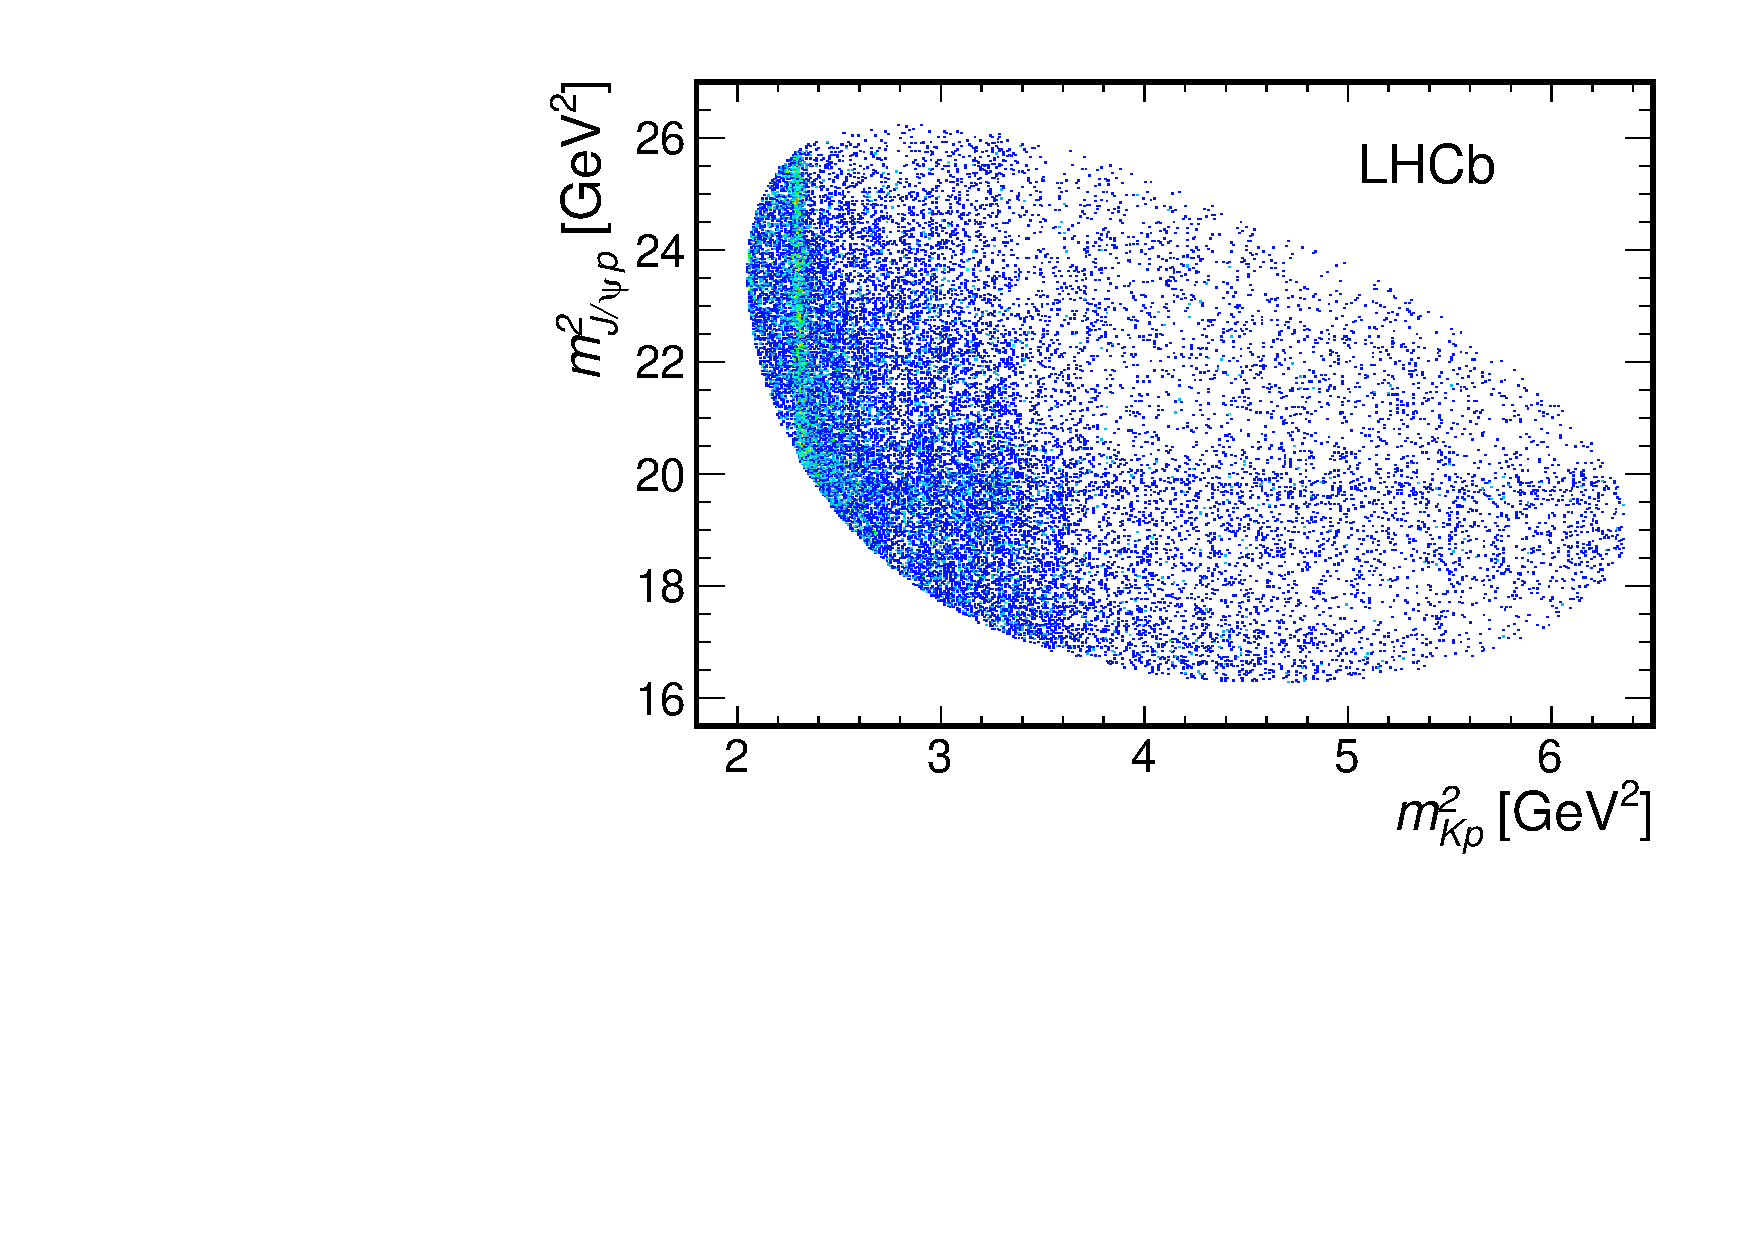
\includegraphics[width=0.48\textwidth]{Figures/01_Introduction/Exotic/Pc_states/2015-lhcb-Lb2jpsipK-dalitz} %
   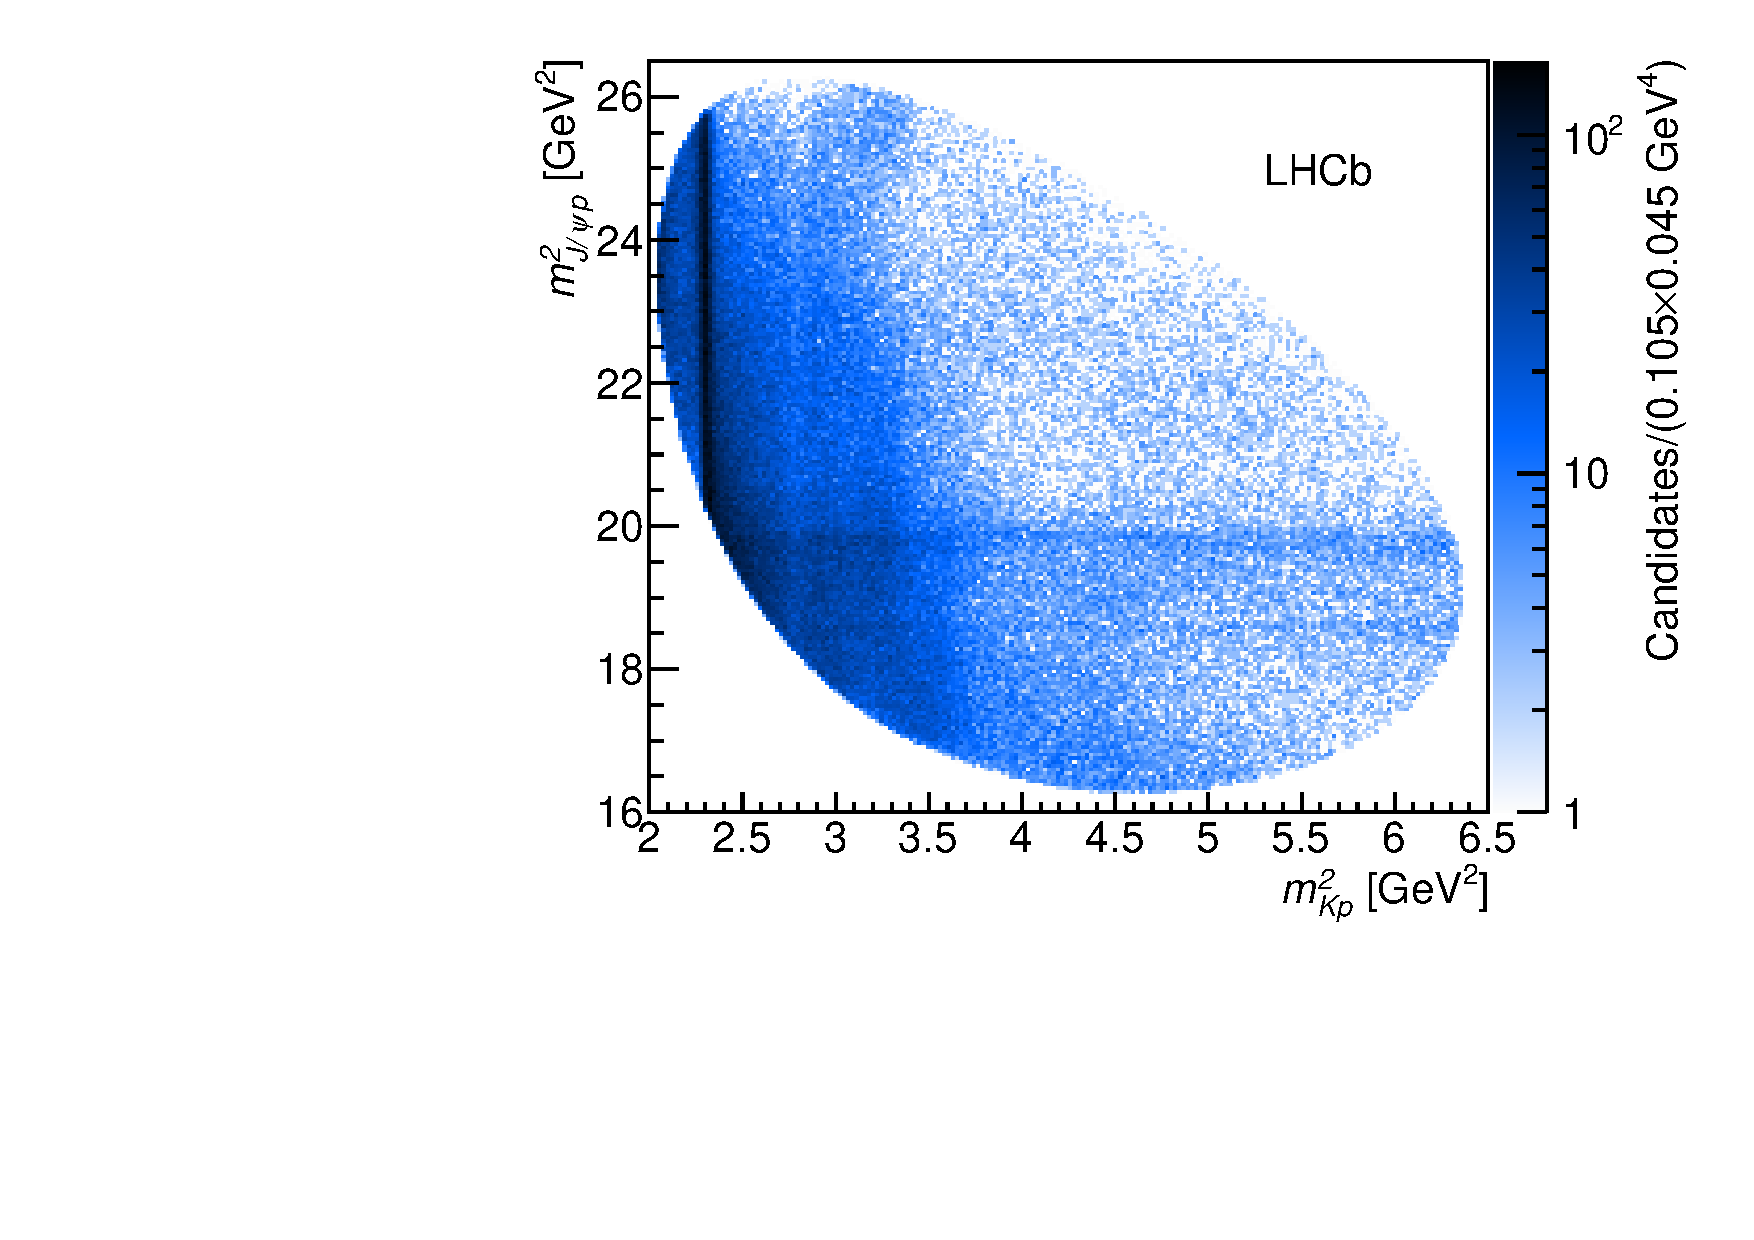
\includegraphics[width=0.43\textwidth]{Figures/01_Introduction/Exotic/Pc_states/2019-Dalitz_plot_pc} %
   \caption{ 
   Dalitz plot of $\Lb\to\jpsi\proton\Km$ with Run 1 data sample (left)\supercite{LHCb-PAPER-2015-029}, 
   with Run 1 and Run 2 data sample together (right)\supercite{LHCb-PAPER-2019-014}.}
\label{fig:Pc_dalitz}
\end{figure}

We then updated $\Lb\to\jpsi\proton\Km$ based on the combined data set collected by the \lhcb collaboration in Run 1,
with $\proton\proton$ collision energies of $7$ and $8 \tev$ corresponding to a total integral luminosity of $3 \invfb$,
and the Run 2 samples with $\proton\proton$ collision energies of $13 \tev$ corresponding to $6 \invfb$\supercite{LHCb-PAPER-2019-014}.
In this updated analysis,
the selection procedure is optimized,
which helps to improve the $\Lb$ reconstruction efficiency  by alomost a factor of two 
and leaves the background level almost unchanged,
detiails of selection procedure are introduced in Appendix.~\ref{app:pentaquark_jpsipk}.
The invariant mass distributions are consistent to the previous study according to the Dalitz plots,
as shown in Figure.~\ref{fig:Pc_dalitz}.
Besides,
performing a rigorous amplitude analysis of this new data sample is computationally challenging.
Therefore,
we applied binned fits to the 1-dimentional distribution $m_{\jpsi\proton}$ distribution,
as shown in the right of Figure.~\ref{fig:Pc_mass}.
Using the nine-fold increased $\Lb$ sample,
the previous reported $P_{c}(4450)^+$ peak is confirmed and resolved into two narrow states,
$P_{c}(4440)^+$ and $P_{c}(4457)^+$.
A narrow $P_{c}(4312)^+$ is discovered with $7.3\sigma$ significance.

Since all three states are narrow and below the $\Sigma_{c}^{+}\Dzb$ and $\Sigma_{c}^{+}\Dstarzb$ thresholds 
within plausible hadron-hadron binding energies, 
they provide the strongest experimental evidence to date for the existence of bound states of a baryon and a meson. 
According to some theorical models\supercite{PhysRev.134.B1307,PhysRevC.98.045208,MAIANI2018247,Bugg_2008,PhysRevD.91.051504},
several other $P_{c}^+$ states should exist.
We expect more structures will be observed at \lhcb with a larger data sample. 


\begin{figure}[!hbtp]
\centering
   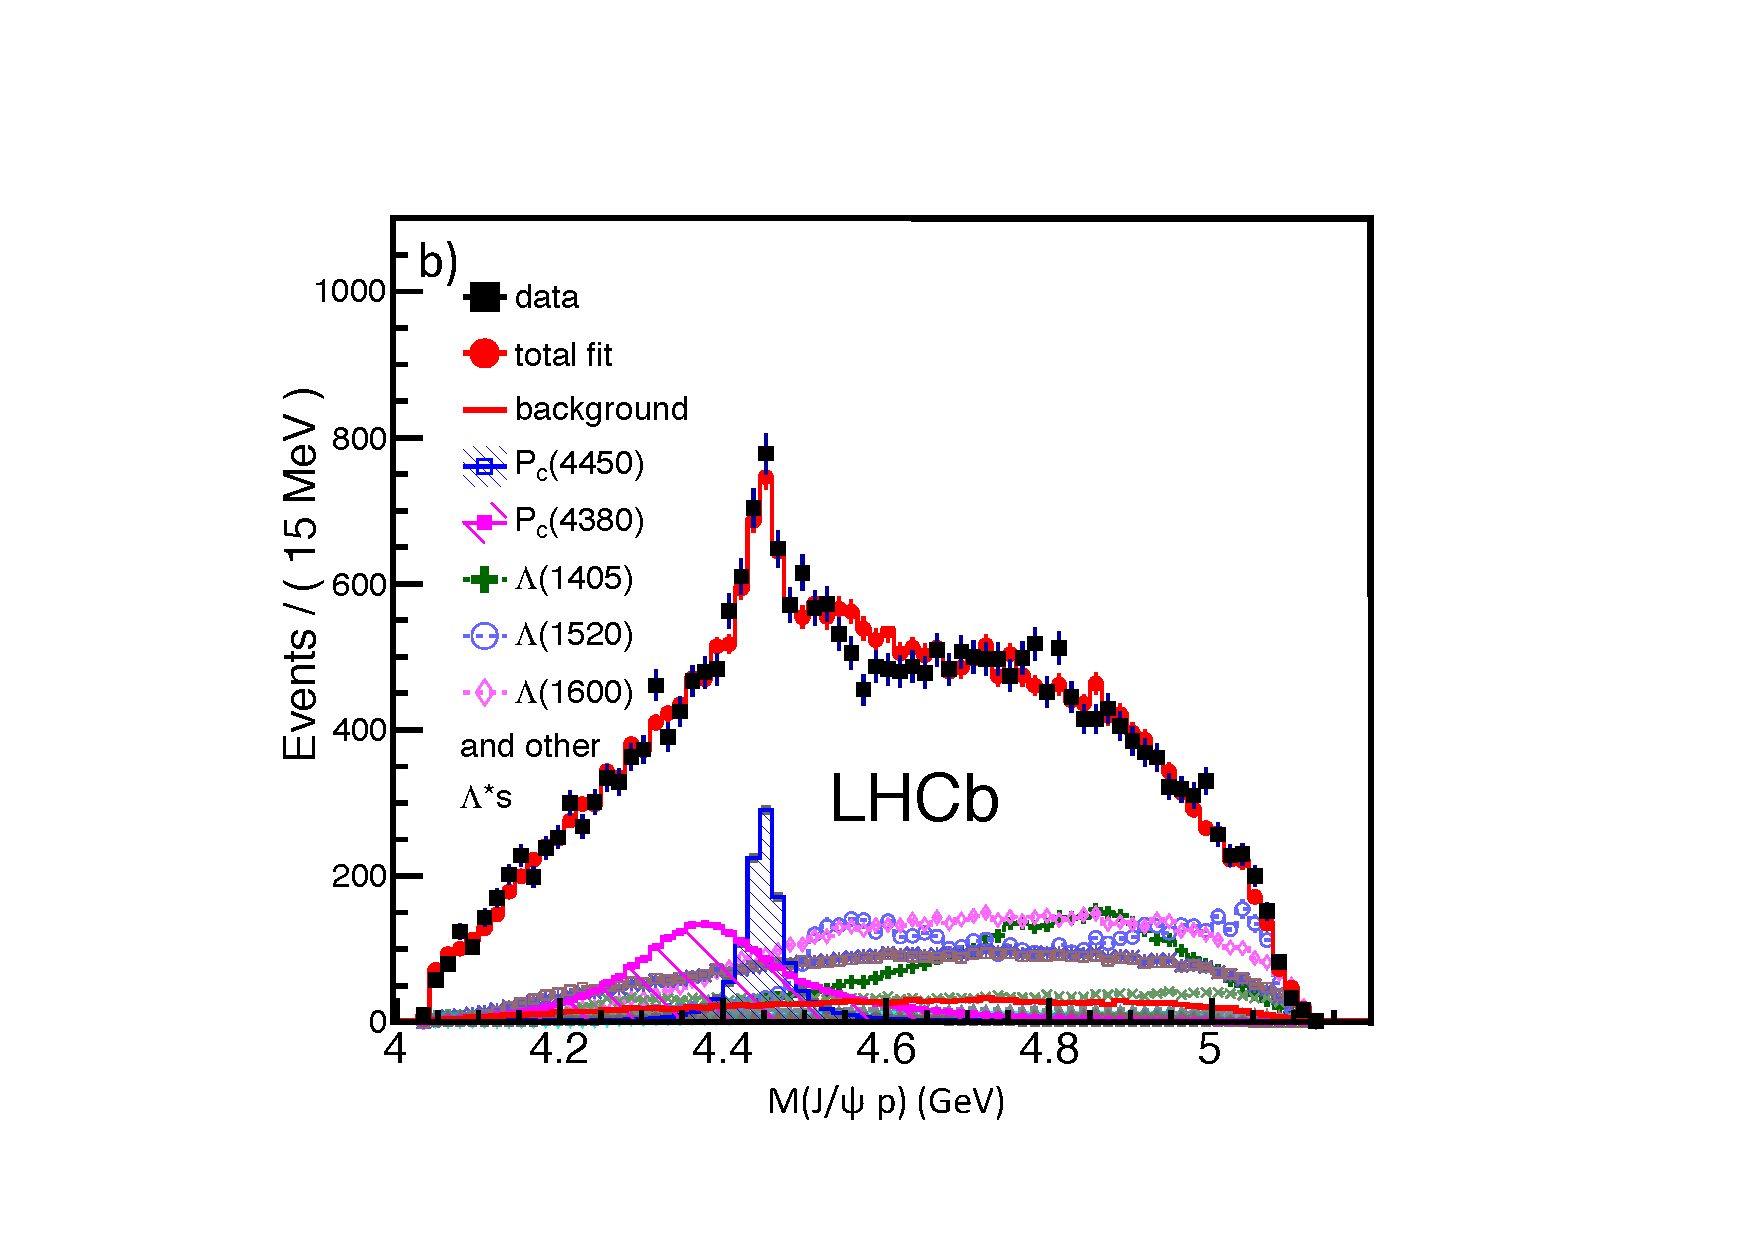
\includegraphics[width=0.46\textwidth]{Figures/01_Introduction/Exotic/Pc_states/2015-lhcb-Lb2jpsipK-mjpsip-default-slo} %
   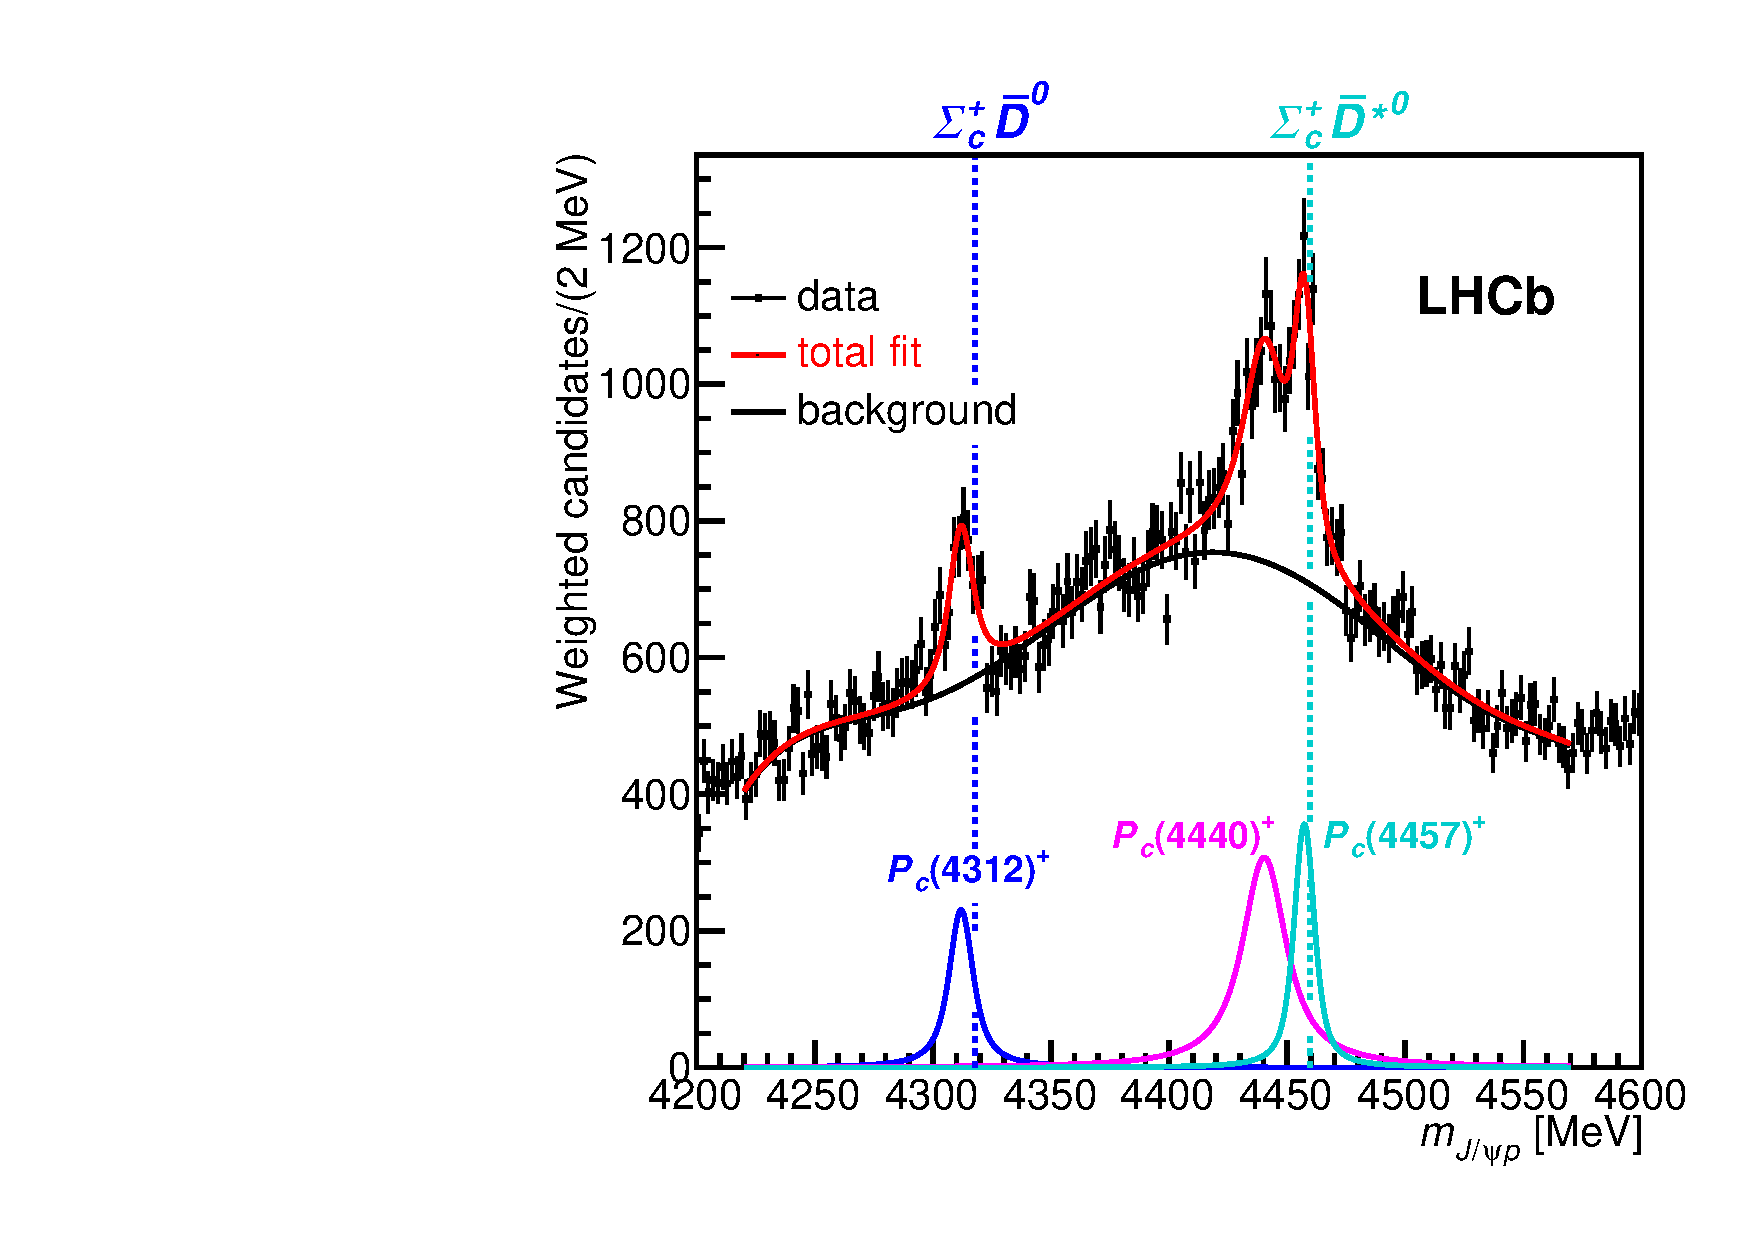
\includegraphics[width=0.44\textwidth]{Figures/01_Introduction/Exotic/Pc_states/2019-pentaquarks_nominal_fit_and_thresholds} %
   \caption{ 
   Fit projection for $m_{\jpsi\proton}$ with two $P_{c}$ states (left)\supercite{LHCb-PAPER-2015-029}.    
   Fit to $m_{\jpsi\proton}$ distribution with three BW discribed $P_{c}$ states (right)\supercite{LHCb-PAPER-2019-014}. }
\label{fig:Pc_mass}
\end{figure}

The Cabibbo-suppressed decay $\Lb\to\jpsi\proton\pim$ was also inspected at \lhcb with Run 1 sample\supercite{LHCb-PAPER-2016-015}.
From a 6-dimentional amplitude analysis,
$3.1\sigma$ evidence for summed presence of $P_{c}(4380)^+$, $P_{c}(445)^+$ and $Z_{c}(4200)^{-}$ is obtained.
The $m_{\proton\pi}$ and $m_{\jpsi\proton}$ projections of the fit are compared in Figure.~\ref{fig:Pc_jpsipi}.
Due to the ambiguities between $P_{c}^+$ and $Z_{c}^-$ terms,
any individual exotic state cannot be confirmed from this study.
Furthermore,
the previous amplitude model should be updated,
since three $P_{c}^+$ candidates are observed from the updated ananlysis at \lhcb\supercite{LHCb-PAPER-2019-014}.
We expect more significant conclusions can be obtained from the updated analysis of $\Lb\to\jpsi\proton\pim$.
The selection optimization of this channel has been finished,
and detailed progresses are introduced in Appendix.~\ref{chap:pentaquark_jpsippi}.

\begin{figure}[!hbtp]
\centering
   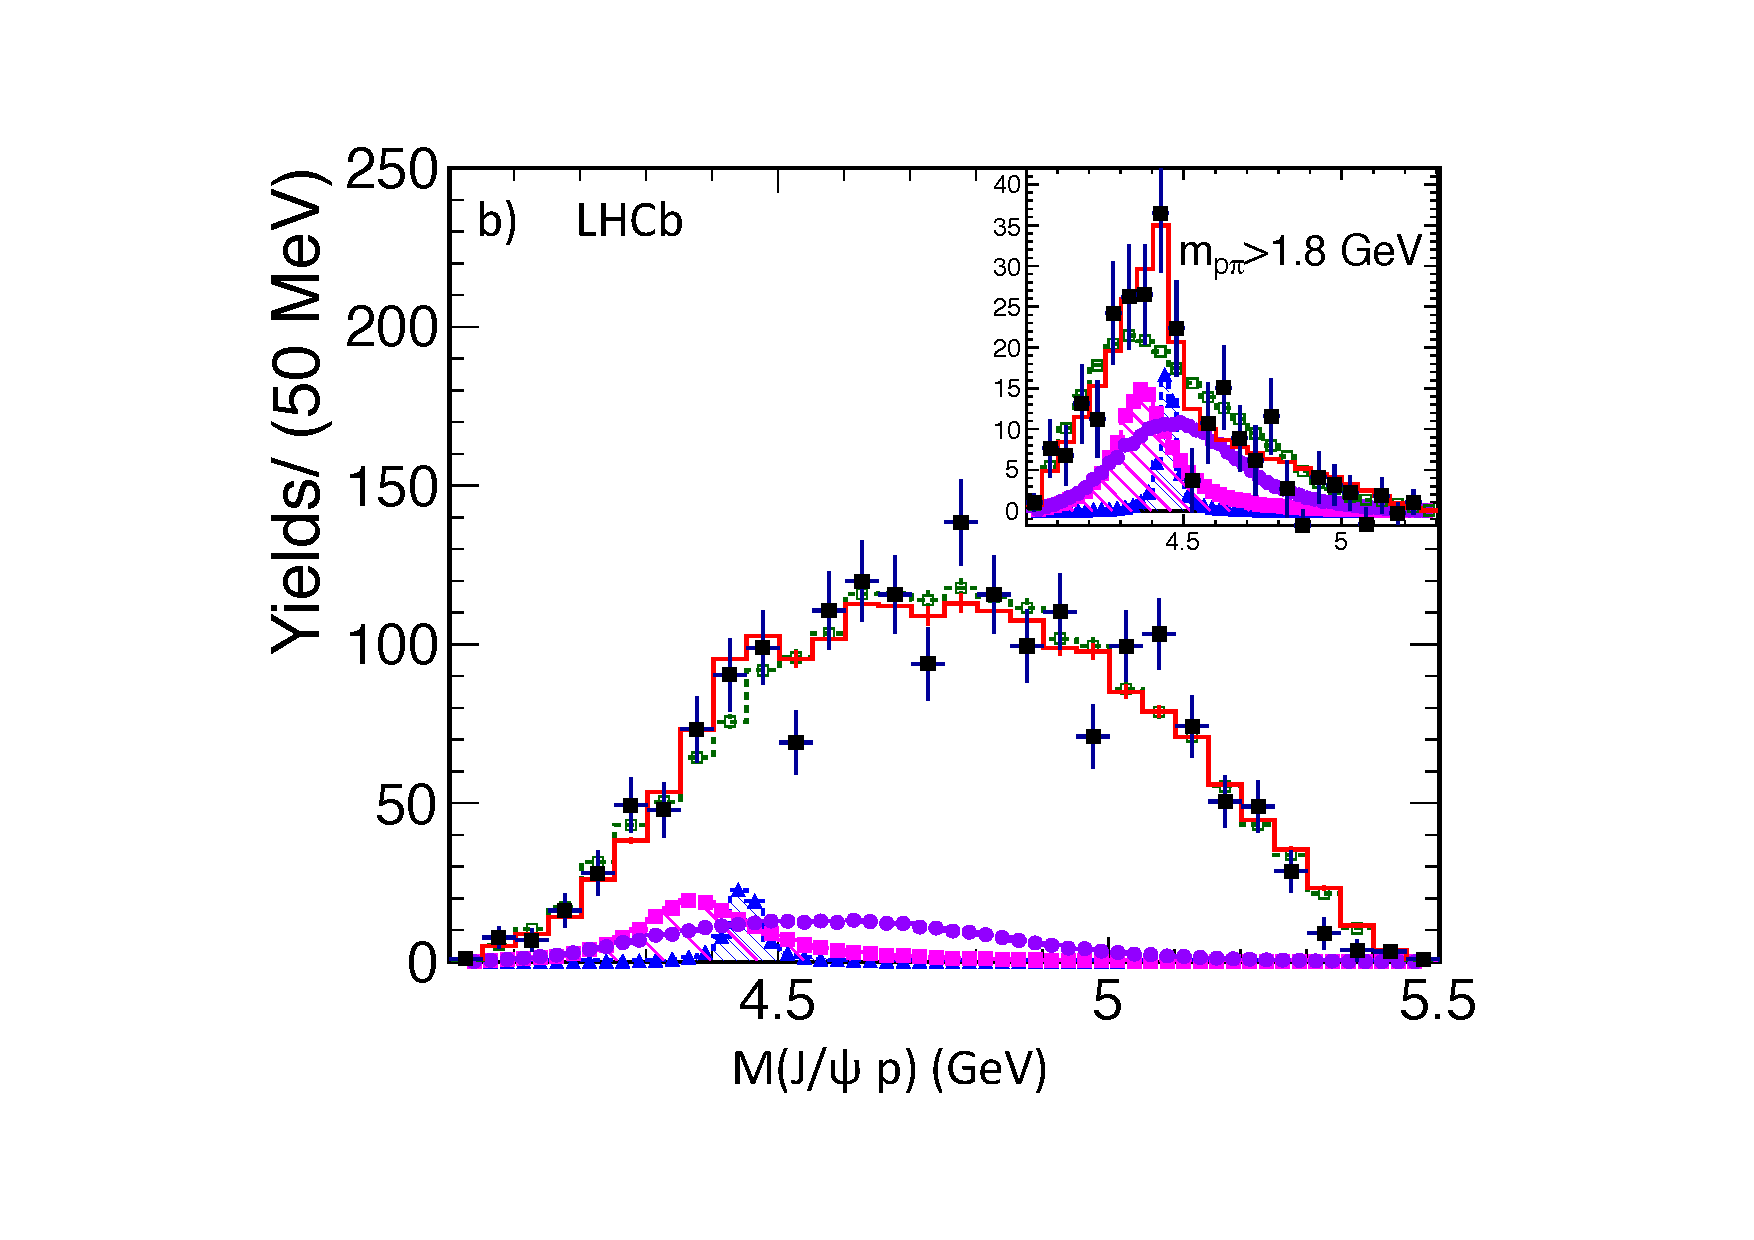
\includegraphics[width=0.45\textwidth]{Figures/01_Introduction/Exotic/Pc_states/lhcb-Lb2jpsippi-mjpsip-inset-slo} %
   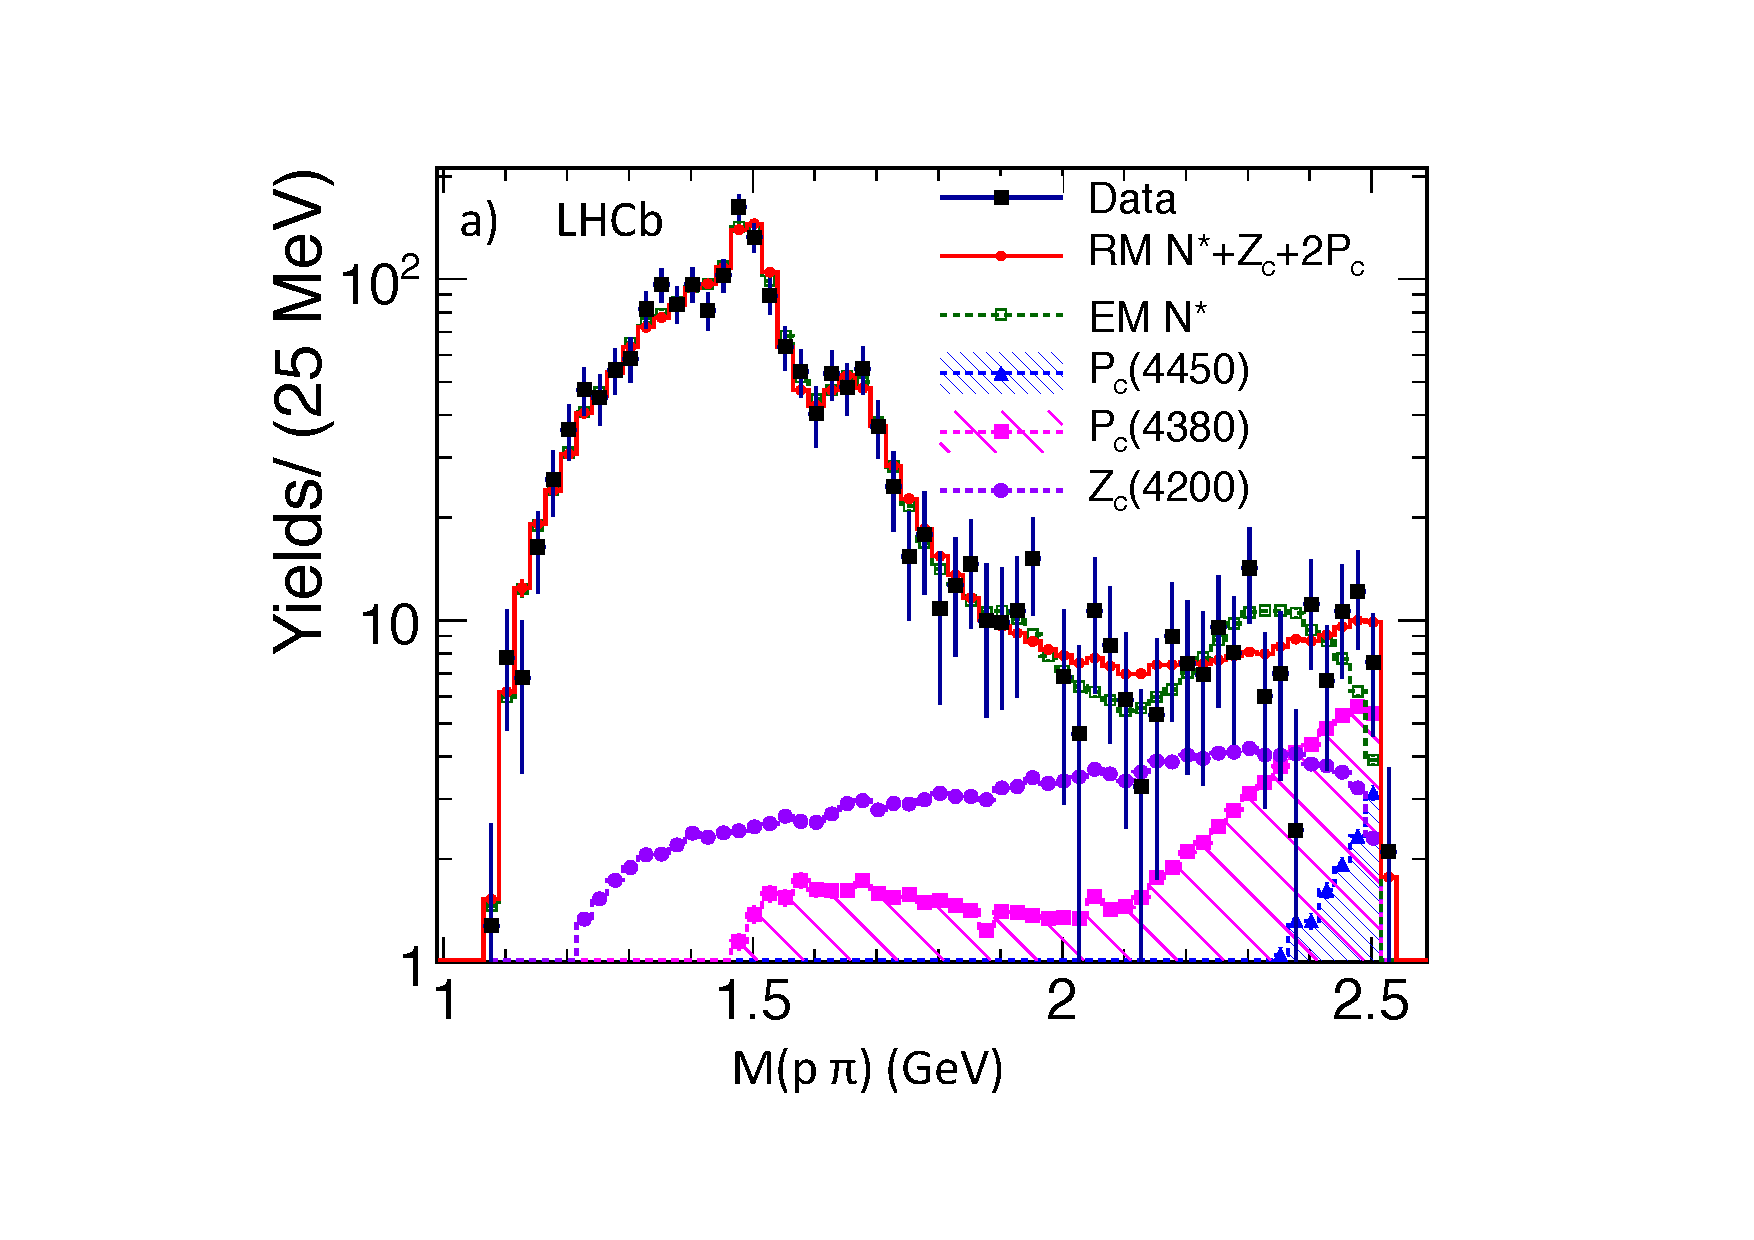
\includegraphics[width=0.44\textwidth]{Figures/01_Introduction/Exotic/Pc_states/lhcb-Lb2jpsippi-mppi-slo} %
   \caption{ 
   Projections of the amplitude fit onto $m_{\proton\pi}$ (left) and $m_{\jpsi\proton}$ data distribution for $\Lb\to\jpsi\proton\pim$ decay 
   in \lhcb\supercite{LHCb-PAPER-2016-015}.}.
\label{fig:Pc_jpsipi}
\end{figure}

The open-strange pentaquark states are searched in $\Xibm\to\jpsi\Lc\Km$ decay at \lhcb\supercite{LHCb-PAPER-2020-039},
and its significance exceeded $3\sigma$.
The $P_{cs}(4459)^0$ state has a mass only about 19 \mev below the $\Xicz\Dstarzb$
threshold and a narrow width. 
Motivated by this fact, 
the hypothesis of two resonances contributing to the enhancement is tested.
The data cannot confirm or refute the two-peak hypothesis. 


























    
%\section{Multiquark states containing strangness}
%\label{section:comments_in_introduction}
%
%The theoretical predictions for strangeness $Z$ states are discussed in  Ref.~\supercite{Chen:2013wca,Ferretti:2020ewe,Lee:2008uy,Voloshin:2019ilw,Dias:2013qga}.
%
%
%\section{Open charm multiquark states}
%\label{section:comments_in_introduction}
%
%The theoretical predictions for strangeness $Z$ states are discussed in  Ref.~\supercite{Chen:2013wca,Ferretti:2020ewe,Lee:2008uy,Voloshin:2019ilw,Dias:2013qga}.



\section{Theoretical models of multiquark states}

Many theoretical models are constructed to explain the exotic hadrons observed in experiments\supercite{LIU2019237}.
The first-principle strategy to treat these observations is lattice QCD,
where the path integral is achieved by transcribing the relevant integrals to a lattice of discrete space-time points.
This is a rigorous method to test the consistency between experimental discoveries and QCD principle,
but the realistic lattice QCD computations require extreme computational resources,
which makes it very hard to perform lattice QCD computing.
Some simplified models are introduced below.


\subsection{Multiquark states as molecules}

The molecule model thinks the multiquark states are meson-meson or meson-baryon molecule-like systems 
that are bound via Yukawa-like nuclear forces, 
and bound states comprised of quarkonium cores surrounded by clouds of light quarks and gluons.
Later, the coupled-channel effect, various hyperfine interactions and recoil corrections were introduced into the one-boson-exchange model step by step. 
Within this model, 
the hidden-charm molecular type pentaquarks were predicted. 
In 2019, 
LHCb collaboration updated their analysis with a ten times larger data sample, 
which strongly supports the molecular pentaquarks. 
At present, 
the idea with one boson exchanged between meson-meson or meson-baryon is an popular way to treat many exotic hadronic interactions.
Nevertheless,
this model sometimes lacks the definite predictive power
as too many unknown parameters such as the coupling constants and cutoff parameter\supercite{LIU2019237}. 
%The original one-boson-exchange model was proposed for the nuclear force where there exists plenty of experimental data such as the deuteron binding energy and enough nucleon nucleon scattering data, which can be used to fix all the unknown model parameters. 
%In contrast, 
%except the pionic couplings, 
%most of the light meson and heavy hadron interaction vertices remain unknown. 
%Especially, 
%the bound state or resonance solution is very sensitive to the cutoff parameter in the form factor which is introduced to suppress the ultraviolet contribution.

\subsection{Chromomagnetic interaction}
In hadron spectroscopy,
the hyperfine structure is from the spin-related interaction between quarks or between quarks and antiquarks.
The one-gluon-exchange potential auses the mass splittings of the conventional hadrons,
whose color configuration is unique. 
Then,
the Hamiltonian of this model can be constructed with the quark masses included,
which can be used to calculate the exotic hadrons' masses effectively.
The chromomagnetic interaction models play an important role in understanding the multiquark systems,
since this model do catch the basic features of spectra and the mass splittings of hadrons reply on the basic controlling symmetries of the quark world.

\subsection{Hadrocharmonium}
In hadrocharmonium picture, 
a compact color-singlet $Q\bar{Q}$ charmonium core state is treated as “blob” of light hadronic matter. 
These two components interact via QCD versions of the Van der Waals force,
and the mutual forces in this configuration are strong enough to form bound states 
if the light hadronic matter is in a highly excited resonant state. 
In this model, 
decays to the hidden charmonium core state are enhanced to a level 
where they are competitive with the mode decaying to open-charm final particles\supercite{DUBYNSKIY200982}. 



\subsection{Rescattering-induced kinematic effects}


While the classic signal for the presence of an unstable hadron resonance is a peak in the invariant mass distribution of its decay products, 
not all mass-spectrum peaks are genuine hadron states,
since some peaks are produced by near-threshold kinematic effects.
These include threshold cusps and anomalous triangle singularities\supercite{RevModPhys.90.015003}.
The threshold cusp may be observed when  the intermediate two particles must rescatter into final states with a lower threshold.
On the the other hand,
the triangle singularity appears in three-body decay,
when the three virtual particles that form the triangle are all simultaneously on the mass shell\supercite{GUO2020103757}.














    % Copyright (c) 2014,2016,2018 Casper Ti. Vector
% Public domain.

\chapter{LHC and \lhcb }
\label{chap:lhcb}
%\pkuthssffaq % 中文测试文字。

The data collected from proton-proton collisions is used in this disseration,
which is generated by the Large Hadron Collider(LHC) and collected in LHCb experiment,
so a brief overview of LHC and \lhcb during Run 1 and Run 2 will be given in this chapter.
Currently, 
the \lhcb sub-detectors are being upgraded for higher luminosity situation in the following Run 3 era, 
the \upgradeone scenario for each subdetector will also be mentioned.  
As this disseration includes some \ecal simulation results for \lhcb \upgradetwo,
more detailed description related to \lhcb calorimeter system will be reviewed in this chapter.

\section{The large hadron collider}

LHC, 
an international project at the European Organization for Nuclear Research (CERN) laboratory in Geneva, Switzerland, 
is the most powerful particle accelerator ever constructed. 
It produces the highest energy particle beams ever created, 
making it the premier facility in the world for research in elementary particle physics. 
The LHC consists of a superconducting particle accelerator, 
approximately 27 kelometers in circumference, 
providing two counter-rotating proton beams with a design energy of 7 TeV per beam. 
It can also provide colliding beams of heavy ions, such as lead. 
During 2011 and 2012 (Run1) the LHC operated at 4 TeV per beam because of a limitation in the electrical connections
between the superconducting magnets. 
After the connections were upgraded during a nearly two-year shutdown, 
Run2 began in mid-2015 and lasted to the end of 2018 at 6.5 TeV per beam,
exploring a new energy region not accessible during Run1. 

\begin{figure}[!hbtp]
\centering
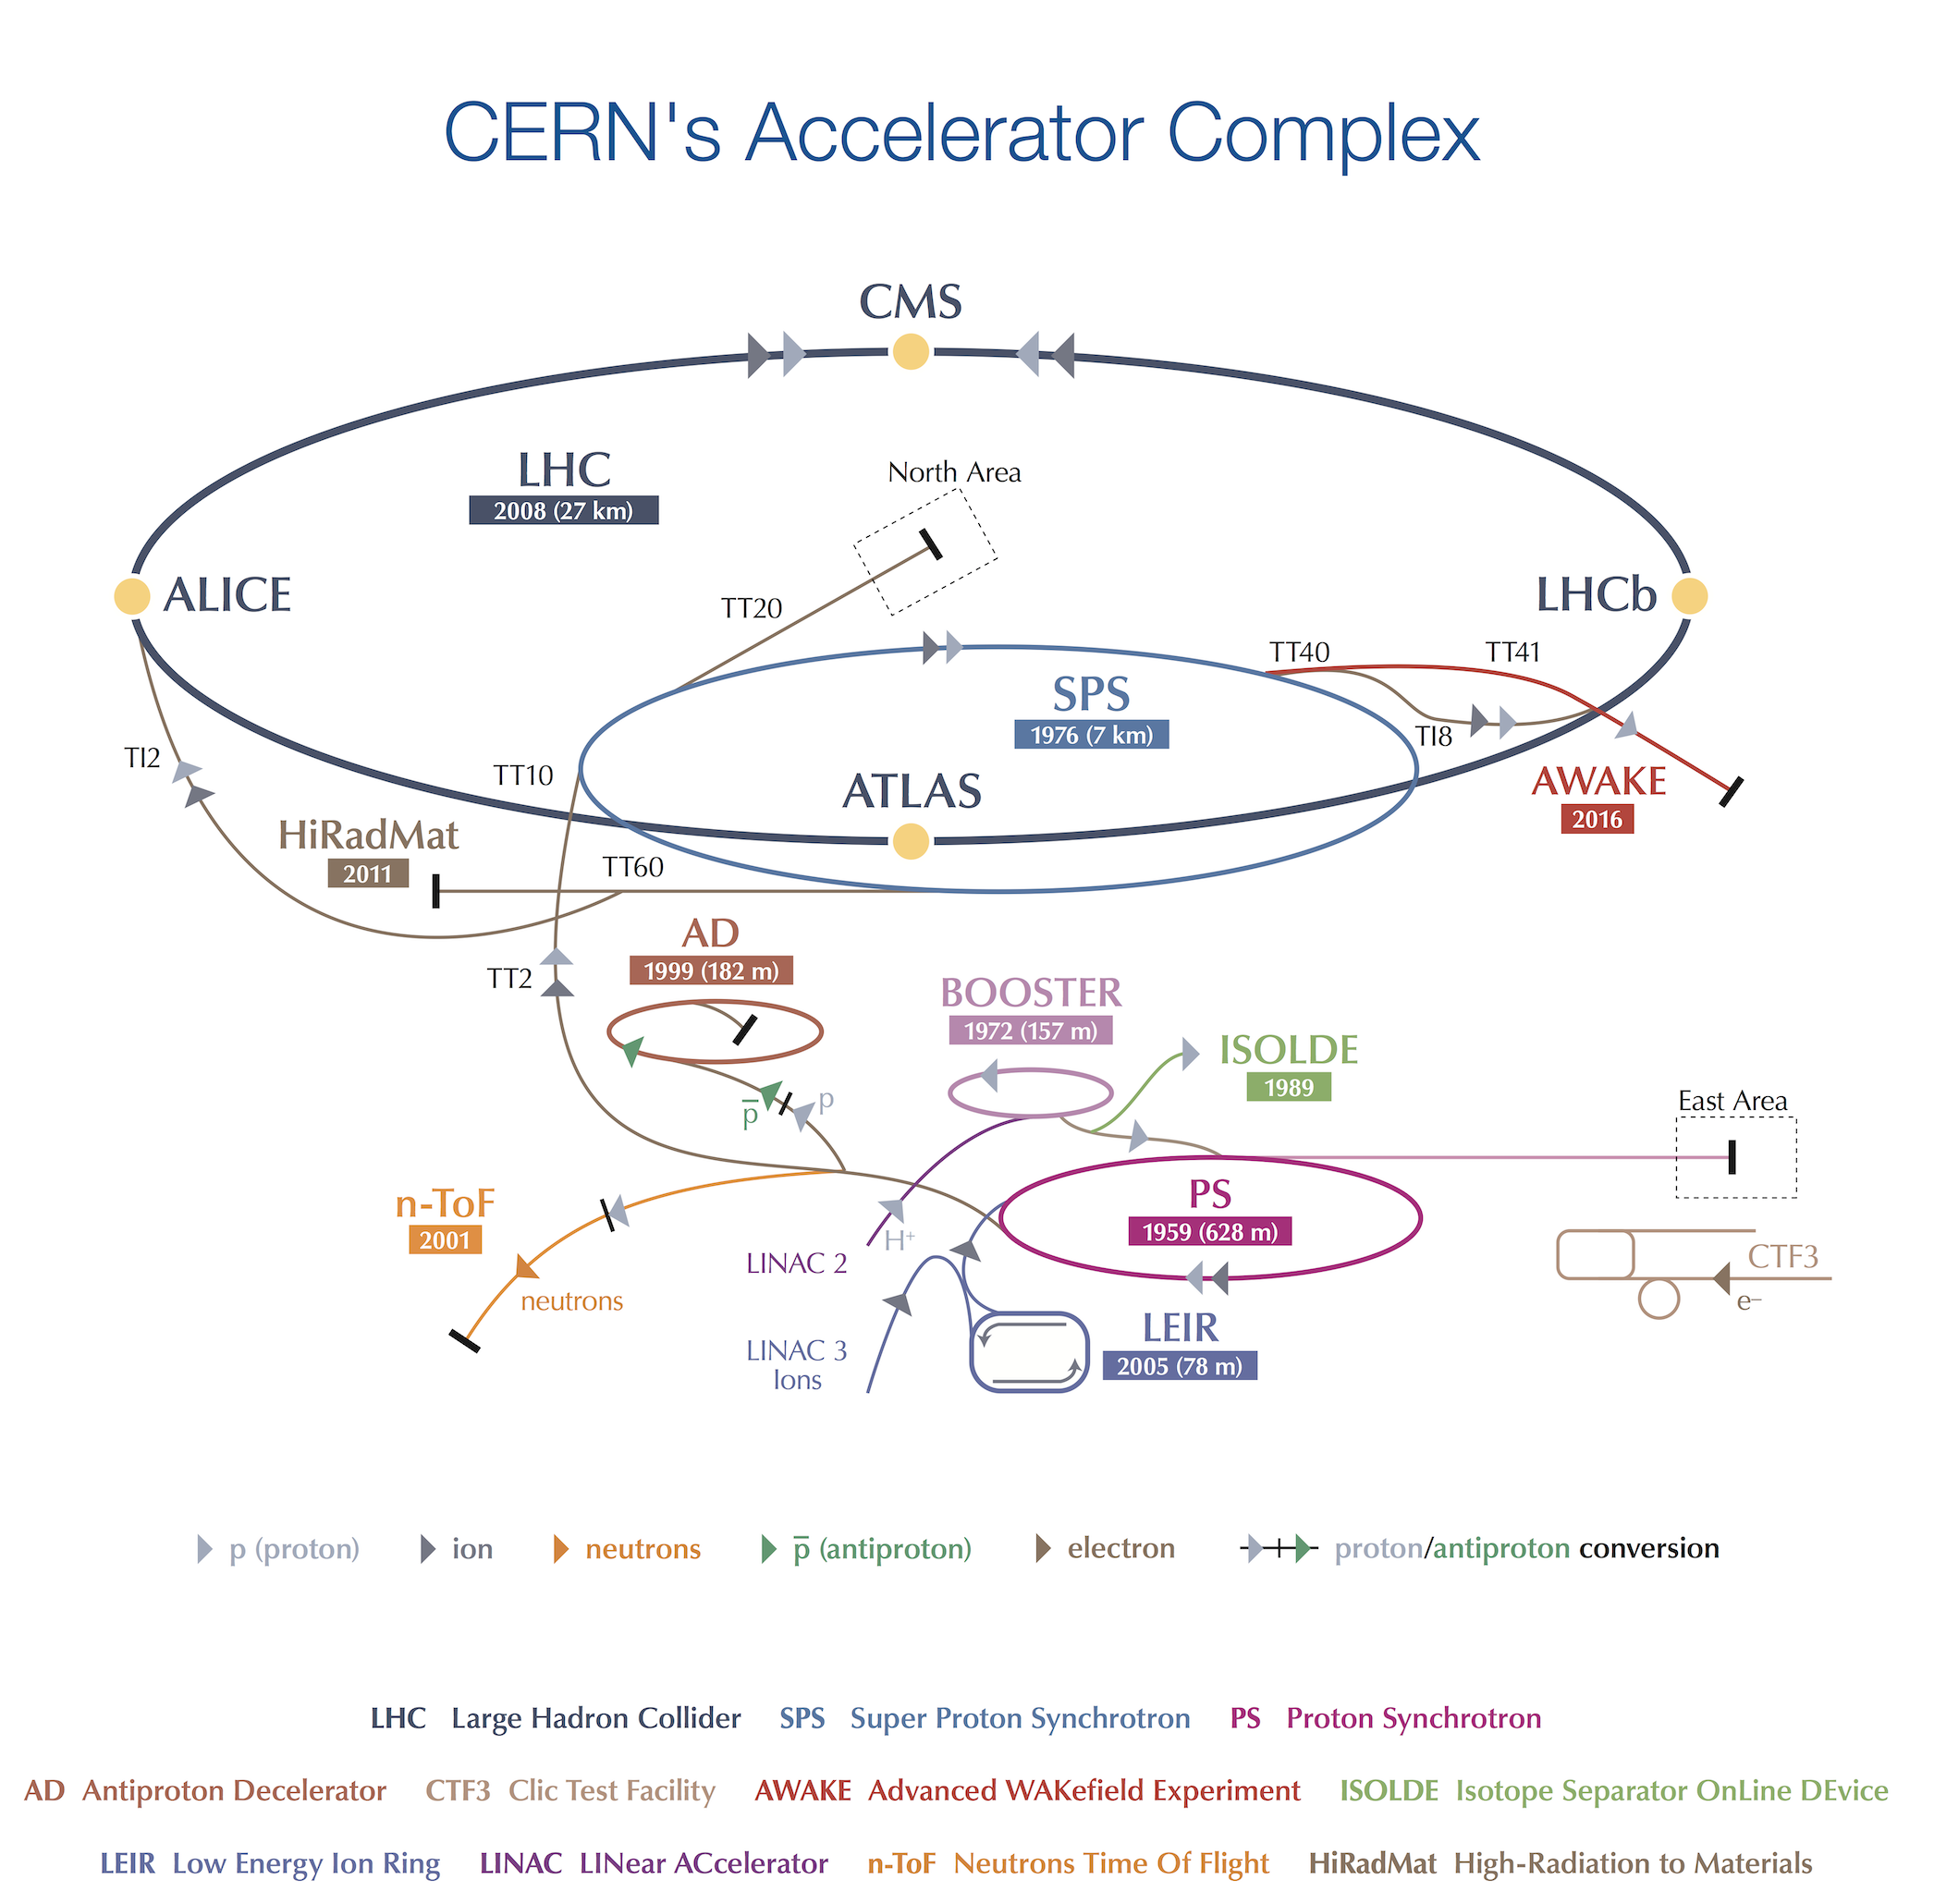
\includegraphics[width=1\textwidth]{Figures/02_Detector/LHC}%
\caption{The CERN accelerator complex.
The LHC is the last ring (dark grey line) in a complex chain of particle accelerators. 
The smaller machines are used in a chain to help boost the particles to their final energies and provide beams to a whole set of smaller experiments, 
which also aim to uncover the mysteries of the Universe\supercite{Haffner:1621894}.}
\label{fig:LHC}
\end{figure}


Actually, 
the LHC is the last element of accelerator complex at CERN,
which is a succession of machines that accelerate particles to increasingly higher energies, as shown in Figure.~\ref{fig:LHC}.
Each machine in the complex boosts the energy of a beam of particles, before injecting the beam into the next machine in the sequence. 
Most of the other accelerators in the chain have their own experimental halls where beams are used for experiments at lower energies.

The proton source comes from a simple bottle of hydrogen gas. 
Then, 
electric field is used to strip the electrons in hydrogen atoms to create protons. 
Linac 2, 
the first accelerator in the complex, 
accelerates the protons to the energy of 50 MeV. 
%Afterwards, 
Subsequently,
the beam is then injected into the Proton Synchrotron Booster (PSB), 
which accelerates the protons to 1.4 GeV, 
afterwards, the Proton Synchrotron (PS) pushes the beam to 25 GeV. 
Then, 
protons are sent to the Super Proton Synchrotron (SPS) which accelerates them to 450 GeV.
Finally, 
the protons are transferred to the two beam pipes of the LHC. 
Two beams in LHC circulate clockwise or anticlockwise respectively.
It takes around 4 minutes to fill each LHC ring, 
and 20 minutes for the protons to reach their maximum energy of 6.5 TeV. 
Beams run for several hours inside the LHC beam pipes under normal operating conditions. 
The two beams collide inside four detectors, 
ALICE, ATLAS, CMS and \lhcb, 
in which the total energy at the collision point is equal to 13 TeV.
The accelerator complex is the Antiproton Decelerator and the Online Isotope Mass Separator (ISOLDE) facility, 
and the Compact Linear Collider test area, 
as well as the neutron time-of-flight facility (nTOF). 
It also provides beams to Gran Sasso (CNGS) project for neutino experiment.
Besides,
protons are not the only particles accelerated in the LHC,
In addition to the protons,
lead ions can be accelerated in LHC,
which start from a source of vaporised lead and enter Linac 3 before being collected, 
they then follow the same route to maximum energy as the protons.

\begin{figure}[!hbtp]
\centering
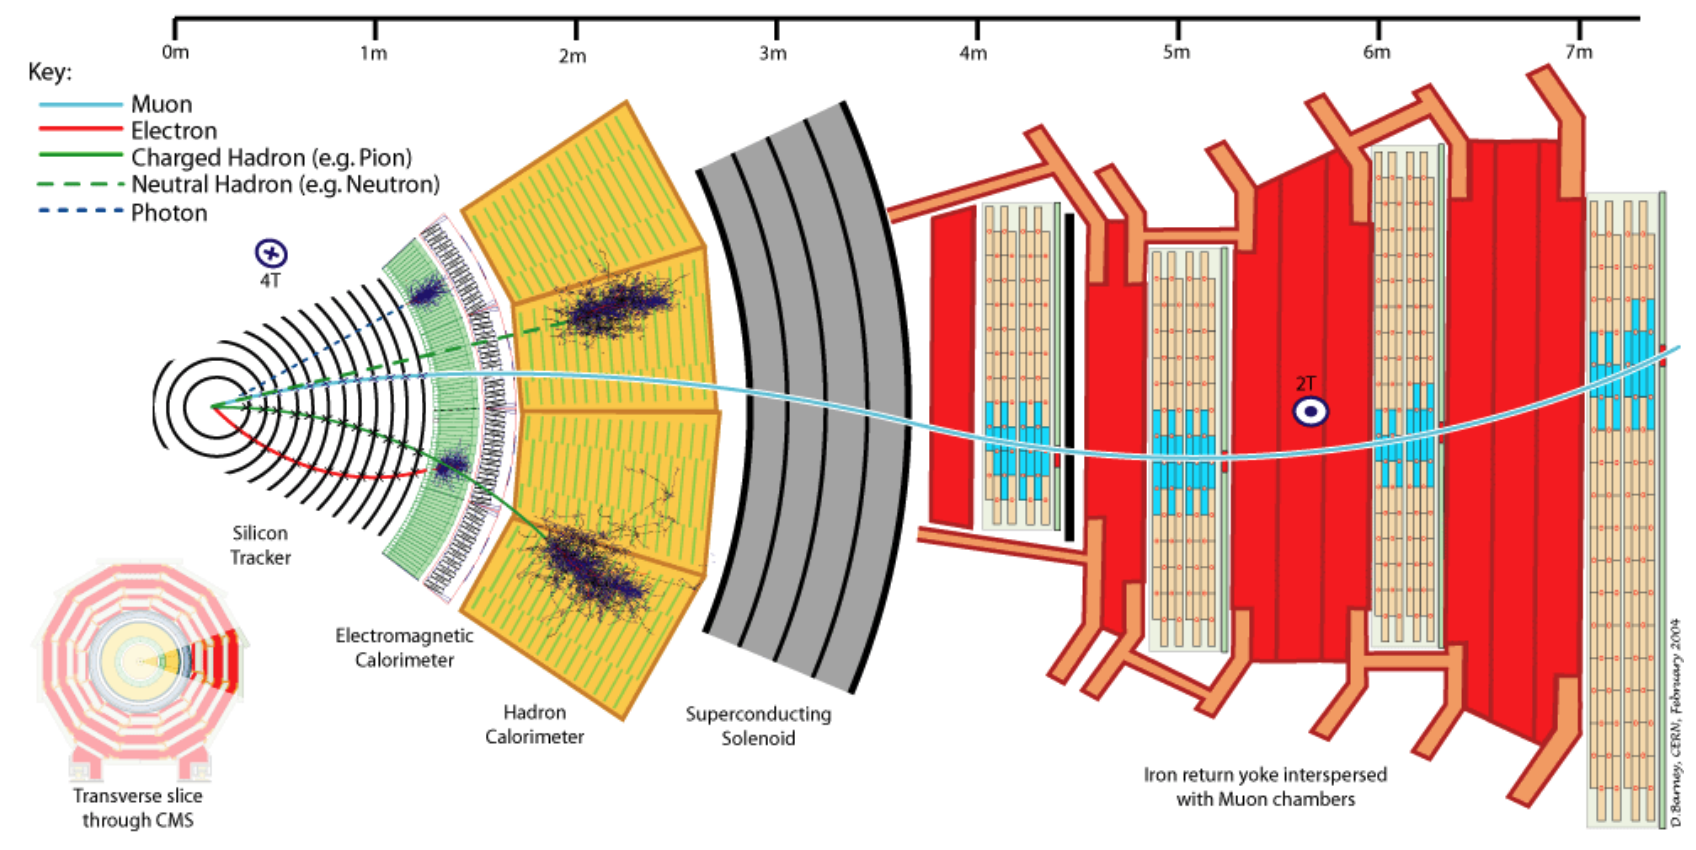
\includegraphics[width=0.7\textwidth]{Figures/02_Detector/CMS}%
\caption{Transverse slice through the CMS detector,
the particle type can be inferred by combining the detector response in the different subdetectors.\supercite{Nielsen_2011}.}
\label{fig:CMS}
\end{figure}

Four main experiments are placed at the LHC. 
Two of them are general purpose experiments, 
studying many aspects of particle productions and decaies. 
These are ATLAS (A Toroidal LHC Apparatus) and CMS (Compact Muon Solenoid) experiments, 
each of them involves more than 3000 scientists and engineers,
in order to search particles beyond standard model directly.
The other experiments, 
each involving around 1000 scientists and engineers, 
and the physical destinations are more specialised: ALICE, (A Large Ion-Collider Experiment) is concerned with heavy-ion collisions, 
and \lhcb (LHC b-hadron experiment) focuses more on the decays of hadrons containing the bottom quark.

These detectors have been constructed as a series of subdetectors, 
and all follow roughly the same scheme,
as shown in Figure.~\ref{fig:CMS},
where the CMS is taken as an example. 
Starting from the inner layers, 
which are positioned closest to the interaction region, 
each detector consists of: 
subdetectors to measure charged-particle trajectories; 
subdetectors to stop photons, 
electrons and hadrons, 
and measure their energies; 
subdetectors to record muons, 
the only charged particles that reach the detector’s outermost layers. 
The ALICE, ATLAS and CMS detectors are approximately cylindrical in shape, 
so as to be sensitive to particles emerging in all directions from an interaction. 
The majority of the particles of interest in \lhcb are emitted at small angles, 
and so the experiment’s detector covers only a narrow cone around the direction of the incoming protons.
In next section, 
the detailed structure of \lhcb will be reviewed.


\section{The \lhcb detector}
LHCb is a single-arm spectrometer with a forward angular coverage from approximately 10 mrad to 300 (250) \mrad,
corresponding to a pseudorapidity range of $1.8 <\eta < 4.9$. 
The layout of the LHCb spectrometer is shown in Figure.~\ref{fig:LHCb}. 
The right-handed coordinate system adopted has the z axis along the beam, and the y axis along the vertical.
This particular geometry of the detector was chosen as the production of \bquark and \bquarkbar quarks at LHC energies 
is such that their directions will tend to be along the beam line.
The polar angles of the \bquark and \bquarkbar hadrons produced for $\sqs=8\tev$ collisions are shown in Figure.~\ref{fig:BBar}, 
as predicted from \pythia8 simulations\supercite{SJOSTRAND2008852},
and similar results apply for pp collisions with the centre-of-mass energy ranging from 7\tev to 14 \tev.
%The choice of the detector geometry is justified by the fact 
%that at high energies both the \bquark-hadrons are predominantly produced in the same forward or backward cone.

\begin{figure}[!hbtp]
\centering
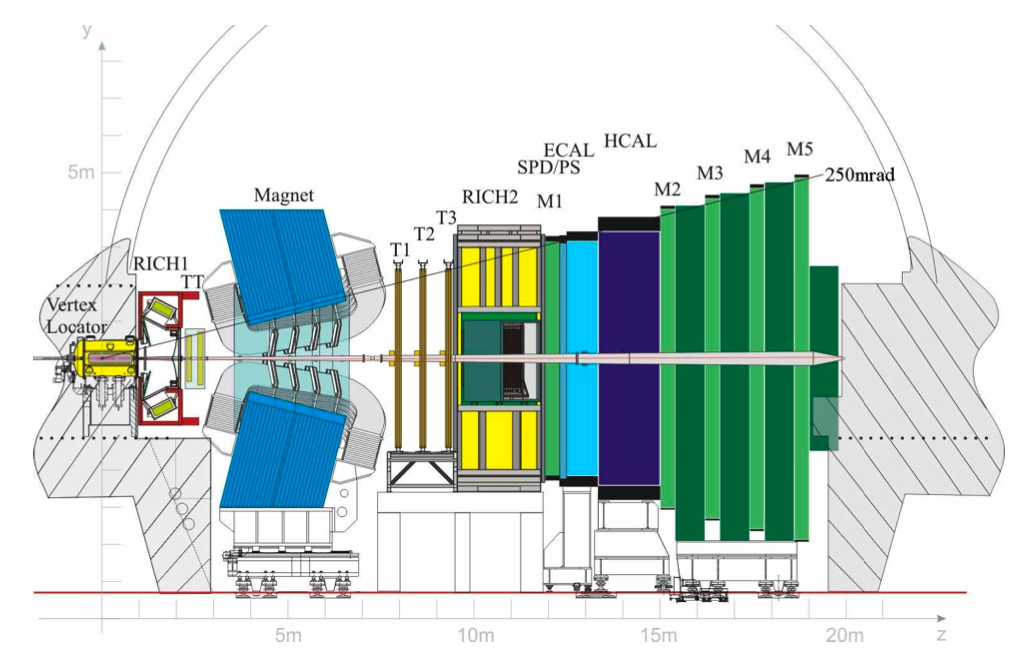
\includegraphics[width=0.95\textwidth]{Figures/02_Detector/LHCb}%
\caption{View of the \lhcb detector\supercite{LHCb-DP-2008-001}.}
\label{fig:LHCb}
\end{figure}

\begin{figure}[!hbtp]
\centering
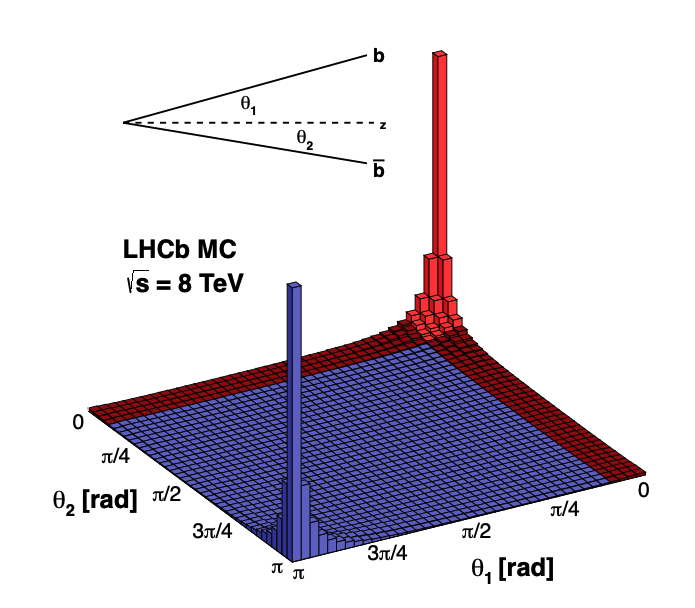
\includegraphics[width=0.65\textwidth]{Figures/02_Detector/BBbar}%
\caption{Display of $\bquark\bquarkbar$ production angles as simulated with \pythia8.
The \lhcb acceptance is shown in red.}
\label{fig:BBar}
\end{figure}

The detector during Run1 and Run2 was designed to operate at a luminosity of $\lum=2\times10^{32}\cm^{-2}s^{-1}$, 
considering the LHC’s design maximum luminosity of $10^{34}\cm^{-2}s^{-1}$, 
a lower luminosity is applied to make for less “busy” events. 
Higher luminosities mean much larger number of interactions per bunch crossing, 
leading to more points where proton-proton collisions take place. 
A proton-proton collision point is also named as a primary vertex (PV), 
and the identification of primary vertices is essential in many analyses in order to accurately reconstruct the paths of decaying particles. 
A high number of primary vertices in an event makes it much more difficult to identify the primary vertex from which a particle originated. 
The higher track multiplicity events, 
which would result from more collisions, 
would also make event reconstruction more difficult. 
Moreover, operating at lower luminosities also limits the radiation damage and detector occupancy. 
A method referred to as “luminosity leveling” is used to achieve the lower luminosity. 
This is done by shifting the beams relative to each other, 
as the number of proton bunches goes down, 
the beams can be made to overlap more in small increments so that the luminosity is also kept constant.

After \upgradeone, 
the liminosity duiring LHC Run3 will be increased to $2\times10^{33}\cm^{-2}s^{-1}$,
which is around 5 times larger than the value in Run2\supercite{LHCb-TDR-012}.
After \upgradetwo,
the luminosity can reach to $1.5\times10^{34}\cm^{-2}s^{-1}$,
total around $300\invfb$ of data will be recorded, 
which offer us an opportunity to take full advantage of the flavour-physics opportunities at the HL-LHC\supercite{LHCb-PII-EoI,LHCb-PII-Physics}.
More comments to \upgradetwo and corresponding the chellange to detector upgrade will be discussed in Chapter\ref{chap:ecal},
especially about \ecal.


\subsection{Tracking}

The tracking system are used to reconstruct charged particles,
and the particles go through tracking subdetectors in proper sequence,
which cantains several parts at \lhcb, 
the Vertex Locater (VELO), 
Diple Magnets and four tracking stations,
as shown in Figure.~\ref{fig:Tracking}.
When comes to the four stations,
one is set in the front of magnet field, 
refered as Tracker Turicensis (TT) and constructed using silicon microstrip sensors,
and other three are located behind the magnet,
known as T1, T2 and T3.
These three stations are divided into inner and outer parts,
the inner section is built by slicon microstrip, 
called as Inner Tracker (IT),
while the outer part is a drift-time dector,
referred to as Outer Tracker (OT).
The following is some details about these sub-detectors.

\begin{figure}[!hbtp]
\centering
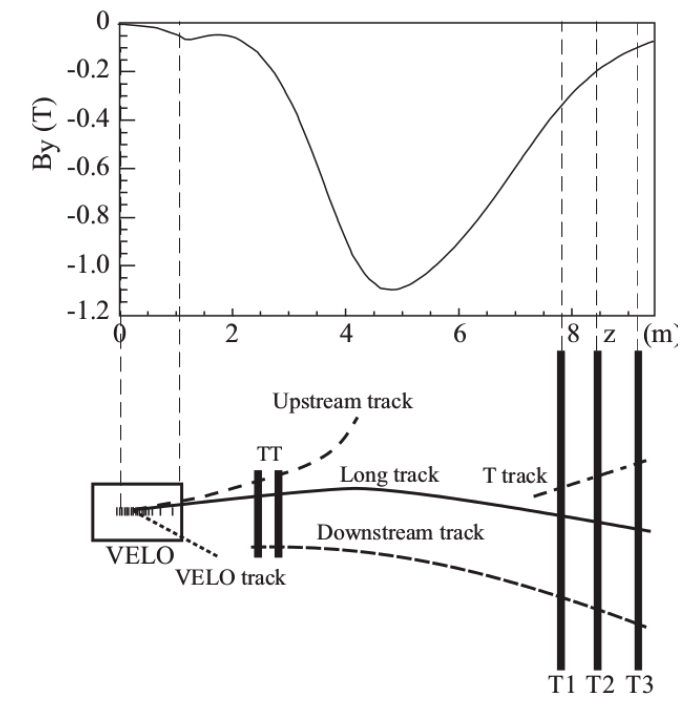
\includegraphics[width=0.65\textwidth]{Figures/02_Detector/Tracking}%
\caption{ Schematic of the tracking compoents with different types of tracking definitions in the tracking reconstruction\supercite{LHCb-DP-2014-002}}
\label{fig:Tracking}
\end{figure}


\subsubsection{Vertex Locater}

The VELO is used to reconstruct the pp collision point,
reconstruct the decay vertices of \bquark and \cquark hadrons and play an important role in second level trigger
\footnote{Details about the trigger at \lhcb will be discussed in Section~\ref{sec:trigger}.}.
For precise vertexing measuremnt,
the VELO should be put as close as possible to the decay vertices,
and make the material between the first measured point and the vertex as less as possible.

The current VELO is constructed by a series of silicon modules, 
each providing a measure of the $r$ and $\phi$ coordinates and perpendicular to the beam direction,
as shown in Figure.~\ref{fig:VELO}.
The VELO includes 25 stations, 
and all of them silicon are placed in vaccum.
Each station contants 2 modules,
positioned on left and right,
as shown in the bottom of Figure.~\ref{fig:VELO}.
Every module has 2 silicon sensors,
one is called $\phi$-measuring sensor,
provides information on the azimuthal coordinate around the beam,
the other sensor,
called the $r$-measuring sensor, 
provides information on the radial distance from the beam axis.
The total number of strips for both sensor types is about 180000 channels.

\begin{figure}[!hbtp]
\centering
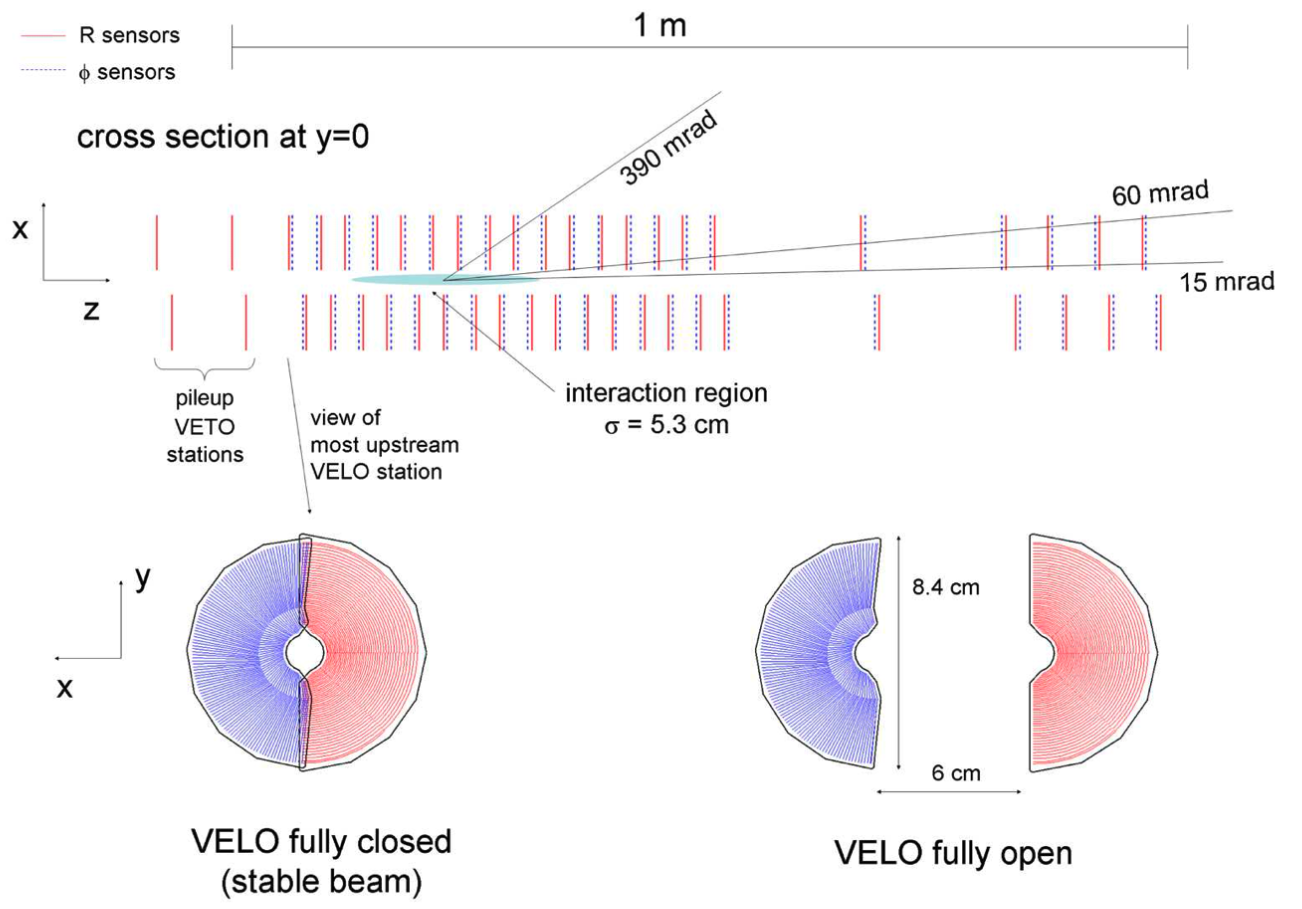
\includegraphics[width=0.85\textwidth]{Figures/02_Detector/VELO}%
\caption{ Overview of the VELO as seen in the (x, z) plane, at y=0, at top. 
	The front face of the modules in the (x,y) plane, for both closed (left) and oprn (right) positions, at bottom\supercite{LHCb-DP-2008-001}.}
\label{fig:VELO}
\end{figure}

Many auxiliary system is designed to keep \velo running normally.
As \velo dector is running in extreme radiation environment with strongly non-uniform fluences,
the sensors are required to maintaining at a temperature between -10 and 0 \degc to counteract the radiation effects, 
The cooling system use two-phase \cotwo to transfer heat by a conventional freon cooler,
which is transfered via a 60 \m long line.
Besides, 
in order to reduce beam-induced effects,
the dectors have to be operated under vaccum,
actually,
fully vacuum condition is not unrealizable,
a vaccum around $10^{-4} \mbarn$ is required.
The dedicated valves and restrictions are used to maintain the vaccum situation,
which are activated by membrane switches that react at the desired pressure difference. 
Another intersting system is known as movement system,
which is used to adjust the distance between \velo and interaction points.
Before the LHC ring is filled, 
\velo has to move away,
when the pp clusters running stable,
the \velo need to be placed into an optimized position,
and this position is not exactly known beforehand.

Currently, 
\lhcb \upgradeone is ongoing for Run3 with higher luminosity.
The new pixel dector with pixel pitch of 55 \mum  will be utilized,
and this kind of detector cannot lead to ghost tracks.
Besides,
totally new front-end electronics are included,
a thin aluminium radio frequency foil is used to make the detector closer to the interaction points\supercite{Svihra:2727215}.


\subsubsection{Dipole Magnets}


A dipole magnet is applied to measure the momentum of charged particles,
which inlcudes two separate aluminum coils, 
shaped like a saddle and mounted symmmetrically in a window-frame magnetic yoke. 
Each coil has fifteen pancakes arranged in five triplets,
and the conductor has a specific ohmic resistance below $28 \Omega\dot\m$ at 20 \degc.
An overview of the magnet can be seen in Figure.~\ref{fig:MAG}.
The magnetic field is vertically in the y-direction, 
and covers the acceptance ±250 mrad vertically and ±300 mrad horizontally. 
The total magnetic field for tracks of 10 m in length is 4 Tm. 
In order to achieve a good momentum resolution, 
the integrated magnetic field must have a very precision value, 
which is on the order of $10^{4}$. 
This precision was achieved using arrays of hall probes, 
with which the components of the field were measured in a fine grid spanning from the interaction point to the RICH2 detector. 
In order to study the detector asymmetry,   
the polarity of the magnet is also able to be reversed. 


\begin{figure}[!hbtp]
\centering
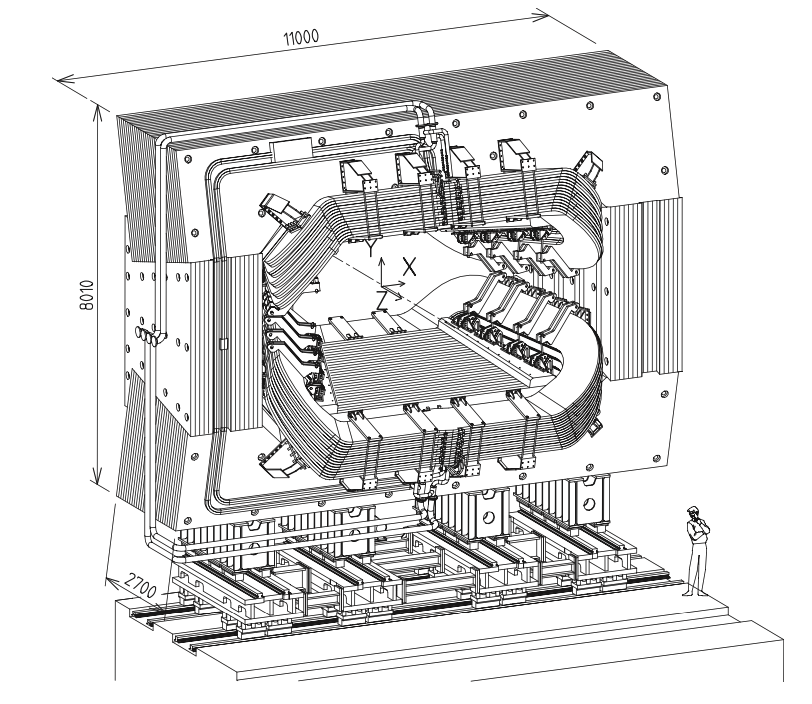
\includegraphics[width=0.75\textwidth]{Figures/02_Detector/MAG}%
	\caption{ Perspective overview of dipole magnet(units in \mm)\supercite{LHCb-DP-2008-001}}
\label{fig:MAG}
\end{figure}



\subsubsection{Silicon Tracker}

Silicon tracker are used in Tracker Turicensis (TT) and the Inner Tracker (IT),
which are constructed by silicon microstrip sensors with a strip pitch of about $200\mum$.
The \ttracker is a planar tracking station, 
which is located upstream of the \lhcb dipole magnet and covers the full acceptance of the experiment, 
as shown in the top of Figure.~\ref{fig:UT}.
The \intr refers to the center region of the three tracking stations downstream of the magnet,
which is 120 \cm wide and 40 \cm, 
as shown in the bottom of Figure.~\ref{fig:UT}.

\begin{figure}[!hbtp]
\centering
\includegraphics[width=0.7\textwidth]{Figures/02_Detector/UT} \\%
\includegraphics[width=0.65\textwidth]{Figures/02_Detector/IT}%
	\caption{ Overview of the TT (top) and IT (bottom)\supercite{LHCb-DP-2008-001}}
\label{fig:UT}
\end{figure}

The basic building blocks of the TT layers are half modules, 
which cover half of the acceptance and are joined together end-to-end in order to create the full module. 
The half modules are made up of seven silicon sensors, 
which are organized into either two or three readout sectors, 
depending on the proximity to the beampipe. 
The read-out sectors have one, two, three, or four sensors bonded together, 
such that the sectors closer to the beampipe, 
which encounter the higher particle flux, 
have the lower number of sensors bonded together. 
The space above and below the beampipe are each covered by a half module, 
and the regions to the sides are covered by rows of seven full modules in the first two layers and eight full modules in the last two layers. 
To avoid acceptance gaps, adjacent modules are staggered by about 1 \cm in z to allow overlap by a few millimeters in x. 
For the u and v layers, individual modules are rotated by the respective stereo angle. 

The three \intr stations consist of four detector boxes arranged around the beampipe.
A detector box contains four detection layers which are arranged in the same ($x-u-v-x$) configuration as the \ttracker. 
Each of the detection layers has seven silicon modules. 
Acceptance gaps are avoided by having adjacent modules staggered by 4 \mm in the z direction and an overlap by 3 \mm in the x direction. 
The modules in the top and bottom boxes consist of a single silicon sensor, 
while the modules in the side boxes consist of two silicon sensors.


\subsubsection{Outer Tracker}

To keep the costs low, 
the \intr is enclosed by the Outer Tracker (\ot), 
which is a large area straw-tube detector, 
and detects about $70\%$ of the charged particles tracks that are produced inside the LHCb acceptance. 
It has a lower granularity than the ST due to the lower activity in the outer regions. 
Same as the ST it consists of four layers in an (x−u−v−x) arrangement. 
The OT provides excellent momentum resolution which is necessary for the precise determination of the invariant mass of the reconstructed b-hadrons. 
The front-end electronics measure drift times of ionisation clusters produced by charged particles traversing the straw tubes, 
which is translated into hit position. 
Figure.~\ref{fig:TT} shows the three \ot stations which comprise two layers of circular straws with an inner diameter of 4.9 \mm. 
The straws are filled with a mixture of Argon ($70\%$), CO2 ($28.5\%$) and O2 ($1.5\%$) 
to ensure a fast drift time below 50 ns and a sufficient drift-coordinate resolution (200 \mum).

\begin{figure}[!hbtp]
\centering
\includegraphics[width=0.99\textwidth]{Figures/02_Detector/TT}%
   \caption{ Left: The three \ot stations surrounding the three \intr stations (purgple). 
	Right: Overview of the \ot bridge carrying the C-frames\supercite{LHCb-DP-2008-001}}
\label{fig:TT}
\end{figure}


All tracking detectors are being upgraded for Run 3. 
The upstream tracker (UT) will use silicon strip technology with improved segmentation and acceptance,
and the total structure is similar to the current one.
The sensors have finer granularity comparing to TT to cope with an increased particle density. 
Sensor strips are vertical to have precise measurement in the horizontal direction,
the direction that charged tracks bend in the dipole magnet.
Each plane is constructed from 16 columnar structure called "staves",
which most have 14 sensor modules,
and mounted alternatively on the front and the back surfaces of its support structure\supercite{LHCb-TDR-015,Proceedings:2015ihx,Rudolph:2020zeq}.

The tracking stations downstream of the magnet will be replaced with a scintillating fiber (SciFi) system during \upgradeone,
which is a total different detector comparing to OT.
The SciFi tracker consists of three stations each with four detection planes. 
The detector is built from individual modules ($0.5\m\times4.8\m$), 
each comprising 8 fibre mats with a length of 2.4\m as active detector material. 
The fibre mats consist of 6 layers of densely packed blue-emitting scintillating fibres with a diameter of 250\mum. 
The scintillation light is recorded with arrays of state-of-the-art multi-channel silicon photomultipliers (SiPMs). 
A custom ASIC is used to digitize the SiPM signals. 
Subsequent digital electronics performs clustering and data-compression before the data is sent via optical links to the DAQ system. 
To reduce the thermal noise of the SiPM, 
in particular after being exposed to a neutron fluence of up to $1012\neqcmcm$, 
expected for the lifetime of the detector, 
the SiPM arrays are mounted in so called cold-boxes and cooled down by 3D-printed titanium cold-bars to $-40\degc$
\supercite{LHCb-TDR-015,Massafferri:2020dbk}.



\subsection{Particle identification}

The purpose of the particle identification (PID) system is to identify the different particle species that travel through the LHCb detector. 
In \proton\proton collisions at the LHC predominantly pions are produced, 
hence it is crucial to distinguish them from the other particle types. 
Information from the Ring Imaging Cherenkov detectors is used to distinguish the charged final state hadrons - kaons, pions, and protons. 
The calorimeters provide information to identify and measure the energy of photons, electrons and hadrons.
The muon detectors are employed to detect and measure muons.


\subsubsection{\rich}

The Ring Imaging CHerenkov (RICH) detectors at LHCb are based on the principle of Cherenkov radiation. 
Cherenkov radiation occurs when a charged particle travels through a medium faster than the speed of light in that medium. 
Cherenkov photons are emitted in a cone shape with opening angle $\theta_{c}$ with respect to the direction of the particles momentum as
\begin{equation}
	cos(\theta_{c}) = \frac{1}{n\beta}
\label{eq:RICH}
\end{equation}
where $n$ is the refractive index of the medium and $\beta=v\/c$, 
where $v$ is the velocity of the particle and $c$ is the speed of light in a vacuum. 

The \rich detectors constains \richone and \richtwo, 
amimg to identify charged tracks with low momentum and high momentum respectively.
The \richone detector is positioned between the \velo and the \ttracker. 
It covers the full angular momentum and provides PID for particles between $1-60\gevc$.
The photodetector planes are split into two halves, 
one above the beam line and one below the beam line. 
The \richtwo covers the full LHCb angular acceptance.
The \richtwo sub-detector is placed between the third tracking station and the first muon station. 
It successfully distinguishes particles with momenta between 15 and 100 \gevc. 
Since high momentum particles are less bent by the magnet, 
the \richtwo detector covers a smaller angular acceptance of 15 mrad up to 100 (120) mrad in the vertical (horizontal) plane. 
The \richtwo Rdetector plane is also made up of two sections, 
placed at either horizontal side of the beam line.
The layout of the \rich detectors is given in Figure~\ref{fig:RICH}. 
The Cherenkov radiation is emitted and reflected out of the detector acceptance by a spherical mirror and a flat mirror. 
They are focused on detection planes, 
where the Cherenkov photons are detected using Hybrid Photon Detectors (HPDs).
Each half of \richone (\richtwo) is equipped with 98 (144) HPDs. 
The particles velocity is reconstructed by identifying rings of Cherenkov photons. 
In combination with the momentum information from the tracking stations, the mass is determined, and the particle can be identified.

\begin{figure}[!hbtp]
\centering
\includegraphics[width=0.85\textwidth]{Figures/02_Detector/RICH}%
   \caption{ Sideview of the \richone detector (Left) and top view of the \richtwo detector\supercite{LHCb-DP-2008-001}}
\label{fig:RICH}
\end{figure}

In order to allow operation of the RICH detector system at the upgrade luminosity,
The \rich detectors is being upgraded by installing new single-photon detectors 
(multianode photomultiplier tubes in place of hybrid photo-detectors) read out by 40 MHz capable electronics, 
and by modifying the upstream RICH optics and mechanics.
The \richone optical system has been redesigned: 
in particular the focal length of the spherical mirrors is increased from 2.7 m to 3.7 m to reduce the hit occupancy on the photodetectors
\supercite{LHCb-TDR-015,FIORINI2020161688}. 
%with the goal of allowing stable operation and easier access to the detector during maintenance.



\subsubsection{Calorimeters}
\label{subsubsec:calorimter}

The main purpose of the calorimeter system is the identification of hadrons, electrons and photons,
and the measurement of their energies and positions.
It is important for calorimeters to enable the reconstruction of $B$-decay channels containing a prompt photon or \piz.
The requirement of a good background rejection and reasonable efficiency for these channels 
adds demanding conditions on the detector performance in terms of resolutions shower separation.

The general structure is that of an electromagnetic calorimeter (\ecal) followed by a hadron calorimeter (\hcal)
as shown in Figure.~\ref{fig:LHCb}.
Besides, 
The scintillator pad detector (\spd) and preshower detector (\presh) are set in the front of \ecal,
the \spd is used to reduce the background for electron trigger,
while the \presh performs to reject the high background of charged particles in \lone trigger.
The \ecal has three zones with different cell size, 
as shown in the left plot of Figure.~\ref{fig:CALO}.
In the inner section, 
the cell size is designed to be close to the Moliere radius, 
which leads most of the energy of a shower deposited in one cell.
The right plot of Figure.~\ref{fig:CALO} shows the lateral segmentation of \hcal, 
which is divided into two zone according to the cell size.
Some propertities to the calorimeter sub-detector are summarized in Table.~\ref{tab:ecal_requirements}.

\begin{figure}[!hbtp]
\centering
\includegraphics[width=0.99\textwidth]{Figures/02_Detector/CALO}%
   \caption{ The lateral segmentation of the \spd$\slash$\presh and \ecal (left) and the \hcal (right) for a quarter of the detector front\supercite{LHCb-DP-2008-001}}
\label{fig:CALO}
\end{figure}

\begin{table}[h]
\caption{Properties of the calorimeter sub-detector.}
\begin{center}
	\begin{tabular}{c| c|c|c}
\hline \hline
sub-detectors  				&   \spd$\slash$\presh  &  \ecal    		& \hcal  			 	\\
\hline 
number of channels			&   $2\times5952$  	&   $5952$  		&   $1468$    		\\  
overall lateral dimension in x,y	&   $6.2\m\times7.6\m$   &   $6.3\m\times7.8\m$  &   $6.8\m\times8.4\m$ 	         		\\
deppth in z					&   $2\Xrad$   		&   $25\Xrad$  		&   $5.6\NIL$  		     		\\
basic requirements			&   \tabincell{c}{$20-30$ photoelectons\\per \mip}  &  \tabincell{c}{$\sigma(E)/E=$\\$10\%/\sqrt{E}\oplus1.5\%$}   	
	   &   \tabincell{c}{$\sigma(E)/E=$\\$80\%/\sqrt{E}\oplus10\%$}  \\
dynamic range				&   $0-100$ \mip  		&   $0-10$\gev \et  	&   $0-10$\gev\et       	\\
\hline \hline
\end{tabular}
\normalsize
\label{tab:ecal_requirements}
\end{center}
\end{table}

The basic principle for current four detectors is 
that the light generated in scintillator is used to measure the energy deposition, 
which is transmitted by wavelength shifting fibers,
the \ecal will be taken as an example to give more details here.

\begin{figure}[!hbtp]
\centering
\includegraphics[width=0.49\textwidth]{Figures/02_Detector/Shashlik}%
\caption{ Shashlik construction of \ecal in the inner zone\supercite{Machikhiliyan_2009}}
\label{fig:Shashlik}
\end{figure}

Figure.~\ref{fig:Shashlik} illustrate the construction of \ecal module used in the inner zone.
To set up this sampling calorimeter module, 
total 66 lead plates and 67 scintillator are used,
with the sampling ratio Pb:Sc is $2:4$ (\mm),
stringed by the wavelength-shifting (WLS) fibers.
The WLS is used to transported the light to the photomultipliers (PM),
which can digitize the light signal.
The digitized signal are processed at 40 \mhz rate by the dead-timeless Front-End electronics.
This kind of module is called as shashlik technology.


After the \upgradeone,
the calorimeter system at \lhcb will become very different.
The present \ecal and \hcal will kept,
while the \presh and \spd will be removed as all trigger will perform in software level
\footnote{More details will be discussed in Section.~\ref{sec:trigger}}.
The \ecal and \hcal front-end electronics will be totally rebuilt,
the PM gain will be reduced by factor of 5 to reduce the PM degradation\supercite{LHCb-TDR-014}.

The \hcal will be removed after \upgradetwo,
and the \ecal will be rebuilt using a total new technology.
The specific scheme of \ecal at LHCb is under consideration,
and more details about this will discussed in Chapter.~\ref{chap:ecal}.




\subsubsection{Moun system}

The final part of the LHCb detector is the muon system which provides the identification
of muons. 
The muon system is made of five stations (M1 to M5) covering an angular acceptance of ±300 mrad in the horizontal plane and ±200 mrad in the vertical plane,
as shown in Figure.~\ref{fig:MUON}.
This corresponds to a geometrical efficiency of approximately $46\%$ for the detection
of muons arising from B hadrons. 
The first muon station, M1, 
is placed before the calorimeters in order to avoid possible multiple scattering effects that could modify the
particle trajectory. 
The remaining stations, M2 to M5, 
are placed after the calorimeter system, 
at the end of the LHCb detector, 
and are separated by iron planes 80 cm thick.
Each muon station is divided into four regions (R1-R4) as shown in Fig. 2.19. 
The R1
region is the closest to the beam-pipe and has the most dense segmentation while the R4 region is the farther. 
The segmentation defined per region is such that the charged particle occupancy is expected to be approximately the same in each region. 
All the muon chambers are composed by Multi-Wire Proportional Chambers, 
except for the inner region of the M1 station, 
which exploits three gas electron multiplier foils sandwiched between anode and cathode planes (GEM detectors). 
In total, the muon system consist of 1368 MWPC and 12 GEM detectors.

\begin{figure}[!hbtp]
\centering
\includegraphics[width=0.65\textwidth]{Figures/02_Detector/MUON}%
\caption{ Sideview of the muon system\supercite{LHCb-DP-2008-001}}
\label{fig:MUON}
\end{figure}

During \upgradeone,
the muon off-detector readout electronics will be redesigned to allow complete event readout at 40 \mhz.
Besides, the M1 before the calorimeter system will be removed\supercite{LHCb-TDR-015,Cardini_2014}.



    

\subsection{Trigger}
\label{sec:trigger}

The nominal instantaneous luminosity is around $2\times10^{32}\cm^{-2}\sec^{-1}$ during Run 1 and Run 2,  
and the rate of events with collisions is roughly 10 \mhz 
when produce at least two charged particles with enough \velo and tracking hits to allow for their reconstruction. 
In fact, 
the rate to storage is about 2-5 \khz,
which is achieved by the trigger system to reduce the rate by selecting only interesting events.
An intial reduction down to 1 MHz comes from the Level-0 (\lone) hardware trigger, 
which uses custom electronics and runs synchronously with the 40 MHz bunch crossing frequency. 
High Level Trigger (\hlt) follows the \lone,
which is a software-base trigger.
The \hlt is subdivided into two stage,
which runs asynchronously on a processor farm and reduces the rate to the desired range. 
The \lhcb trigger scheeme is shown in Figure.~\ref{fig:TRIGGER}.
More details will be given on each stage in the following sections.

\begin{figure}[!hbtp]
\centering
\includegraphics[width=0.99\textwidth]{Figures/02_Detector/TRIGGER}%
\caption{ Flow-diagram of the different trigger sequences\supercite{LHCb-DP-2008-001}.}
\label{fig:TRIGGER}
\end{figure}


\subsubsection{\lone trigger}

The \lone trigger contains three components:
the pile-up system,
the Level-0 calorimeter trigger and the Level-0 muon trigger.
All components are connected to the Level-0 dicision unit (DU) 
which is used to evaluate the final dicision by collecting all the information obtained from the trigger system,
as shown in Figure.~\ref{fig:L0_trigger}.

\begin{figure}[!hbtp]
\centering
\includegraphics[width=0.49\textwidth]{Figures/02_Detector/L0_trigger}%
\caption{ Overview of the \lone trigger\supercite{LHCb-DP-2008-001}.}
\label{fig:L0_trigger}
\end{figure}

The pile-up system is used to distinguish the crossings with single and multiple visible interactions, 
which is based on the silicon sensors in the \velo to measure the radial position of tracks. 
The pile-up system has two functions: 
to provide the position of the primary vertices candidates along the beam-line 
and to measure of the total backward charged track multiplicity.


The calorimeter trigger is designed to search for high \et particles by adding the \et of $2\times2$ cells and selecting the clusters 
with the largest \et,
this step is performed on the Front-End card.
Then the information from \ecal and $\presh \& \spd$ are merged to identifiy the type of electromagnetic candidate, electron, $\gamma$ or \piz.
Besides,
the \et of all \hcal cells is summed to reject crossings without visible interactions. 
The total number of \spd cells with a hit are counted to provide a measure of the charged track multiplicity in the crossing.
%Besides, 
%measurements of the total \et in \hcal and total \spd multiplicity are also performed.

A \lone muon processor is used to search for the two muon tracks with the largest and second largest \pt,
which is performed on the logical pads.
This trigger can look for hits regarded as a straight line through the five muon stations and pointing to the interaction point.
The track position in the first two stations allows the determination of its \pt.
From this system, 
the \pt resolution of a reconstructed stand-alone muon can reach to ~$20\%$.


\subsubsection{\hltone trigger}

The \hltone trigger can reconstruct the trajectories of charged particles traversing full \lhcb tracking system,
besides,
a precision primary vertex reconstruction is perform\supercite{Aaij_2019}
Most particle-identification algorithms cannot be executed in this stage excepting muon identification,
due to a clean signature.
At the same time,
the electrons are identified by associating tracking to \ecal clusters,
photon and neutral pion are also built fromt he clusters reconstructed in the \lone trigger.

The steps of \hltone algorithms is shown in Figure.~\ref{fig:Hltone}.
Firstly, 
the \velo tracks are reconstructed,
as well as the finding of primary vertices.
Then the \velo tracks are extraploted to match the hits in the \ttracker stations to form upstream tracks.
By the way, 
this process can also reduce the number of fake \velo tracks.
Finally, 
the long tracks are reconstructed by combining the information from downstream trackers,
and the search window in the \intr and \ot is defined by the maximum possible function of charged particles with \pt larger than $500\mev$.
The next step is to fit tracks with a Kalman filter to obtain the optimal parameter estimate,
as well as the fake track rejection to removed the tracks with poor quality.

\begin{figure}[!hbtp]
\centering
\includegraphics[width=0.69\textwidth]{Figures/02_Detector/Hltone}%
\caption{Track and vertex reconstruction in the \hltone trigger\supercite{Aaij_2019}.}
\label{fig:Hltone}
\end{figure}

The muon identification in \hltone with all fitted tracks.
For the muon tracks,
the corresponding hits are required in the fout MUON stations,
which is also used in \hlttwo and offline.


\subsubsection{\hlttwo trigger}

In the \hlttwo stage,
the full event reconstruction and identification is performed,
including the charged track reconstruction,
neutral particle reconstruction and particle identification with the information from PID detectors considered.
The corresponding steps of track and vertex reconstruction are shown in Figure.~\ref{fig:Hlttwo}.

\begin{figure}[!hbtp]
\centering
\includegraphics[width=0.69\textwidth]{Figures/02_Detector/Hlttwo}%
\caption{Track and vertex reconstruction in the \hlttwo trigger\supercite{Aaij_2019}.}
\label{fig:Hlttwo}
\end{figure}

In the charged particle reconstruction process,
the \hltone algorithm is repeated firstly,
a second step is to reconstruct the lower-momentum tracks with is overlooked in \hltone.
The track reconstruction becomes larger as low \pt tracks included and no \ttracker hits required.
Besides,
the long-live particles that decay outside the \velo are reconstructed using T-station segments,
which are extrapolated to the magnetic field and combined with hits in the \ttracker.
Next step is to reject fake tracks from the random combination of hits or a mismatch with different tracks segments.
This procedure is based on the Kalman filter and multi-variable analysis tool (TMVA).
Then the remaining tracks are filtered to remove the clone tracks that share enough hits in each subdetector.

The \rich detectors provide the important discrimination between kaons, pions and protons,
and this information can add likelihood for each mass hypothesis to the reconstructed tracks.
The calorimeter system can offer PID information by matching between reconstructed tracks and calorimeter clusters,
combining the information from MUON system,
mature PID values are provided to the tracks.


\subsubsection{Trigger system after \upgradeone}

The most distinguishing feature of trigger after \upgradeone at \lhcb is a full software scheme,
which can offer unprecedented flexbibility in designing selections, 
and in particular allows efficient triggering on low-momentum signatures wich would normally be out of the reach for hadron collider.
The dataflow after \upgradeone is illustrated in Figure.~\ref{fig:Hlt_upgrade}

\begin{figure}[!hbtp]
\centering
\includegraphics[width=0.69\textwidth]{Figures/02_Detector/upgrade_trigger}%
\caption{Dataflow in the upgraded \lhcb detector\supercite{LHCb-TDR-021}.}
\label{fig:Hlt_upgrade}
\end{figure}

%The all trigger system after \upgradeone consists several steps.
%Firstly,
%the data collected from subdecters are processed in event filter farm (EFF) using the RTA applications,

As the \lone trigger is removed,
all the tigger dicisions are based on the \hlt,
which is split into two stages, 
as similar as the strategy in Run 2.
This two stages is seperated by a disk buffer that save data used for alignment and calibration.
The \hltone can reject events contain only poor intesting particles for any \lhcb analysis,
and \hlttwo use the full reconstruction and identification algorithms to obtain the high-level physics objects relevant to analysis for permanent storage.
Many R\&D projects are under way currently,
and some algorithm optimization and code migration tasks have made great advances\supercite{LHCb-TDR-021,LHCb-TDR-018,LHCb-TDR-017,LHCb-TDR-016}.

























	% Copyright (c) 2014,2016 Casper Ti. Vector
% Public domain.
\chapter{Observation of $Z_{cs}$ states in $\Bp\to\jpsi\phi\Kp$ decay}
%\chapter{Dataset, Reconstruction and Selections}
\label{chap:Zcs_study}

%%\section{Previous study and $Z_{cs}$ prediction}
\section{Study motivation}

Since the discovery of the $X(3872)$ state by the \belle experiment in 2003\supercite{PhysRevLett.91.262001}, 
more than twenty non-conventional hadrons that contain $\ccbar$ or $\bbbar$ quarks have been found and studied\supercite{PDG2020}. 
In contrast to the neutral states, 
charged states like $Z_c(3900)^+$\supercite{PhysRevLett.110.252001,PhysRevLett.110.252002} and $Z_c(4430)^+$\supercite{Choi:2007wga, Chilikin:2013tch, LHCb-PAPER-2014-014} provide evidence for tetraquark exotic states, 
because light quarks are required to account for the non-zero electric charge in addition to the heavy quarkonium.
\footnote{Charge conjugation is implied throughout this thesis.} 
Previously, 
only the \uquark or \dquark quarks were observed to constitute the light quark content of such charged exotic states, 
even though the existence of a $Z_{cs}$ state as a strangeness-flavour partner of the $Z^+_c(3900)$ state 
has been predicted\supercite{Voloshin:2019ilw,Dias:2013qga,Chen:2013wca,Ferretti:2020ewe,Lee:2008uy}.
%As mentioned in Section.~\ref{subsubsec:01_Zcs_observation},
Therefore,
it is an important research topic to search the hiddren charm tetraquark with strangeness in hadron spectroscopy field,
the property of this type of states can help test different theoritical predictions to nonstandard hadron states. 
%Besides, the measured widths of $X(4140)$ among different experiments ^ 

\subsection{Previous studies}
%Among all known decays of $b-$hadrons, 
%$\Bp\to\jpsi\phi K^+$ are unique, 
%since conventional hadron contributions from kaon excitations (hereafter denoted as $K^{*+}\to\phi K^+$) are broad, 
%and visible mass structures on the Dalitz plot are dominated by a number of relatively narrow $X\to\jpsi\phi$ states, 
%which are candidates for tetraquarks with hidden-charm and hidden-strangeness. 
%Contributions from these exotic hadron components approach half of the entire rate in this decay channel.
%The first evidence for the $\jpsi\phi$ state was observed by CDF~\supercite{Aaltonen:2009tz}. 
%A very narrow ($\Gamma=15.3_{-\phantom{1}6.1}^{+10.4}\pm2.5$\mev), 
%near-threshold ($M=4143.4\pm3.0\pm0.6$\mev) 
%$X(4140)$ state was claimed.
%\footnote{The recent PDG naming convention calls this state $\chi_{c1}(4140)$. 
%However, 
%generic $X$ label is used for $\jpsi\phi$ states, 
%which is independent of their $J^P$ assignments.} 
%Such narrow structure was not confirmed by the Belle~\supercite{ChengPing:2009vu}, Babar~\supercite{Lees:2014lra}, 
%and early low-statistics LHCb~\supercite{LHCb-PAPER-2011-033} data. 
%However, 
%the near-threshold state was observed by the CMS collaboration~\supercite{Chatrchyan:2013dma}. 
%There was also an evidence for it from the D0 experiment~\supercite{Abazov:2013xda}. 
%An evidence for a second structure, $X(4274)$, in the CDF and CMS data was observed. 
%The $\jpsi\phi$ mass distribution among $2480\pm160$ $\Bp\to\jpsi\phi K^+$ events detected by CMS is shown in Figure.~\ref{fig:newfig3}, 
%which was obtained after the subtraction of a very large combinatorial background.  
%
%\begin{figure}[b]
%  \begin{center}
%  \vspace{-0.3cm}
%   \includegraphics[width=0.4\textwidth]{Figures/01_Introduction/Physics/from_Zcs/newFig3.pdf}
%     \vskip -0.4cm
%    \caption{\small
%The number of  $\Bp\to\jpsi\phi K^+$  candidates as a function
%of $\Delta m = m(\mu^+\mu^-\Kp\Km)-m(\mu^+\mu^-)$.
%    }
%    \label{fig:newfig3}
%  \end{center}
%\end{figure}

%LHCb~\supercite{LHCb-PAPER-2016-018,LHCb-PAPER-2016-019} performed the first amplitude analysis of $\Bp\to\jpsi \phi K^+$ decays, 
%investigating the $\jpsi \phi$ structures in Run 1 data. 
%The number of $\Bp\to\jpsi \phi K^+$ signal events was $4289\pm141$ with a background fraction of $23\%$. 
%The data could be described including seven $K^{*+}\to\phi K^+$ resonances, 
%determined by the fit and consistent with either known or predicted states, 
%four $X\to\jpsi\phi$ structures, and non-resonant $\phi K^+$ and $\jpsi \phi$ contributions. 
%The mass projections of $\phi K^+$ and $\jpsi \phi$ combinations are shown in Figure.~\ref{fig:defmasses}. 
%Table~\ref{tab:run1} shows the results, including the determined masses, widths, fit fractions and spin-parity assignments. 
%The four $X$ structures and a non-resonant $\jpsi \phi$ contribution all had significance above 5$\sigma$. 
%The existence of $\Xtwo$ was established. 
%The quantum numbers of $\Xone$ and $\Xtwo$ states were identified as $1^{++}$ at  $>5\sigma$ significance, 
%while the $\Xthree$ and $\Xfour$ states as $0^{++}$ at $>4\sigma$. Notably, the $\Xone$ width was substantially larger than previously determined. 
%
%\begin{figure}[hbtp]  
%  \begin{center}
%    \includegraphics[width=0.5\textwidth]{Figures/01_Introduction/Physics/from_Zcs/newbase_PhiKh.pdf}%
%    \includegraphics[width=0.5\textwidth]{Figures/01_Introduction/Physics/from_Zcs/newbase_JpsiPhih.pdf} 
%  \end{center}
%\caption{
%    Distributions of $\phi K^+$ (left) and $\jpsi\phi$ (right)
%    invariant masses for the $\Bp\to\jpsi \phi K^+$ candidates (black data points) 
%    compared with the results of the default amplitude fit
%    to the Run 1 data \supercite{LHCb-PAPER-2016-018}.}
%  \label{fig:defmasses}
%\end{figure} 


\begin{table}[h]
\centering
\caption{Results from previous publication based on Run 1 data at \lhcb\supercite{LHCb-PAPER-2016-018}.}\label{tab:run1}

\begin{tabular}{cccccc}
\hline
\multicolumn{2}{c}{Contribution} &Significance & \multicolumn{3}{c}{Fit results} \\
                &                                  &            & $M_0$ [MeV]   & $\Gamma_0$ [MeV]      & FF\% \\
\hline \hline
&      All K($1^+$)   & 8.0$\sigma$       &      &      &  $42\pm 8^{+5}_{-9}$  \\
   &      ${\rm NR}_{\phi K}$  &       &      &      &  $16\pm 13^{+35}_{-6}$  \\
$\nslj{2}{1}{P}{1}$   &    K($1^+$)   & 7.6$\sigma$       &  $1793\pm 59^{+153}_{-101} $   &   $365\pm 157^{+138}_{-215} $   &  $12\pm 10^{+17}_{-6}$ \\
$\nslj{2}{3}{P}{1}$     &    $K^{\prime}$($1^+$)   & 1.9$\sigma$       &  $1968\pm 65^{+70}_{-172} $   &   $396\pm 170^{+174}_{-178} $   &  $23\pm 20^{+31}_{-29}$   \\
\hline
   &       All K($2^-$)   & 5.6$\sigma$       &      &      &  $11\pm 3^{+2}_{-5}$  \\
$\nslj{1}{1}{D}{2}$   &  $K_2 (1770)$     & 5.0$\sigma$       &  $1777\pm 35^{+122}_{-77} $   &   $217\pm 116^{+221}_{-154} $   & \\
$\nslj{1}{3}{D}{2}$ &  $K_2(1820)$   & 3.0$\sigma$       &  $1853\pm 27^{+18}_{-35} $   &   $167\pm 58^{+83}_{-72} $   &   \\       
\hline    
& $K(1^-)$ \\
$\nslj{1}{3}{D}{1}$  &  $K^*(1680)$  &    8.5$\sigma$       &  $1722\pm 20^{+33}_{-109} $   &   $354\pm 75^{+140}_{-181} $   & $6.7 \pm 1.9^{+3.2}_{-3.9}$ \\  
\hline 
& $K(2^+)$\\

$\nslj{2}{3}{P}{2}$  &  $K^*_2(1980)$   & 5.4$\sigma$       &  $2073\pm 94^{+245}_{-240} $   &   $678\pm 311^{+1153}_{-559} $   & $2.9 \pm 0.8^{+1.7}_{-0.7 }$   \\  
\hline 
& $K$($0^-$) \\
$\nslj{3}{1}{S}{0}$  &  $K(1830)$    & 3.5$\sigma$       &  $1874\pm 43^{+59}_{-115} $   &   $168\pm 90^{+280}_{-104} $   & $2.6 \pm 1.1^{+2.3}_{-1.8 }$    \\  
\hline\hline
 & All $X(1^+)$ & & & &$16\pm 3^{+6}_{-2}$ \\
 & $X(4140)$ & $8.4\sigma$ & $4146.5\pm 4.5^{+4.6}_{-2.8}$ & $83 \pm 21^{+21}_{-14}$ & $13.0\pm 3.2^{+4.8}_{-2.0}$\\
 & $X(4274)$ & $6.0\sigma$ & $4273.3\pm 8.3^{+17.2}_{-3.6}$ & $56 \pm 11^{+8}_{-11}$ & $7.1\pm 2.5^{+3.5}_{-2.4}$\\
\hline
 & All $X(0^+)$ & & & &$28\pm 5 \pm 7$ \\
  & ${\rm NR}_{J/\psi \phi}$ & $6.4 \sigma $& & &$46\pm 11^{11}_{-21}$  \\
 & $X(4500)$ & $6.1\sigma$ & $4506\pm 11^{+12}_{-15}$ & $92 \pm 21^{+21}_{-20}$ & $6.6\pm 2.4^{+3.5}_{-2.3}$ \\
 & $X(4700)$ & $5.6\sigma$ & $4704\pm 10^{+14}_{-24}$ & $120 \pm 31^{+42}_{-33}$ & $12\pm 5^{+9}_{-5}$ \\
\hline

\end{tabular}
\normalsize
\end{table}

In Run 1 analysis, $Z_{cs}^+\to \jpsi K^+$ contributions were also tested. 
The results were mentioned in Ref.~[\cite{LHCb-PAPER-2016-019}] and detailed in Thomas Britton's Ph.D. thesis\supercite{ThomasBritton:2016}. 
They are summarized in Table~\ref{tab:hahaha}. 
The improvement for $\jpsi K^+$ mass distribution is shown in Figure.~\ref{fig:jpsikrun1}.  
About $3\sigma$ evidence for a $Z_{cs}^+$ was found, but deemed insufficient to claim discovery of an exotic state with a new quark content. 

\begin{table}[h]
\caption{$Z_{cs}^+$ tests of \lhcb Run 1 analysis\supercite{ThomasBritton:2016}.}
\begin{center}
\begin{tabular}{ccccc}
\hline
$J^P$ & mass [MeV] & width [MeV] & fit fraction & signifiance \\
\hline \hline
$2^+ / 0^-$ & no inform & 4-5 & 0.5-0.6\% & $1.2\sigma/2.5\sigma$ \\
$1^+ / 2^-$ & no inform/($3937\pm7$) & 47/($51\pm15$) & 1.9/2.5\% & $2.5\sigma / 3.1\sigma$ \\
$1^-$ (fit did not converge) & $\sim4220$ & $\sim 500$ & $\sim 10\%$ & \\
\hline
\end{tabular}
\normalsize
\label{tab:hahaha}
\end{center}
\end{table}

\begin{figure}[hbtp]  
  \begin{center}
    \includegraphics[width=0.5\textwidth]{Figures/01_Introduction/Physics/from_Zcs/newbase_JpsiKh}%
    \includegraphics[width=0.5\textwidth]{Figures/01_Introduction/Physics/from_Zcs/Z_JpsiKh}  
  \end{center}
\caption{
    Distributions of  $\jpsi K^+$
    invariant masses for the $\Bp\to\jpsi \phi K^+$ candidates (black data points) 
    compared with the results of the default amplitude fit (left) and amplitude fit with a $Z_{cs}^+$ (right) in Run 1 analysis \supercite{ThomasBritton:2016}. 
	The $Z_{cs}^+$ contribution is shown by large black square point.}
  \label{fig:jpsikrun1}
\end{figure} 

\subsection{This analysis}
In this analysis with full Run 1 and Run 2 data, 
and an improved selection,  
the $\Bp$ signal yield is about 5.5 times of that found in the Run 1 analysis (20\% more signal found in Run 1 data). 
At the same time background fraction is reduced to much smaller level (4\%). 
The improved data sample offers better sensitivity to exotic hadron with smaller contributions. 
Therefore, 
in this analysis we focus on exploring $X\to\jpsi \phi$ sector in more detail, 
as well as on $Z_{cs}^+\to \jpsi K^+$ states. 
%The theoretical predictions for strangeness $Z$ states are discussed in  Ref.~\supercite{Chen:2013wca,Ferretti:2020ewe,Lee:2008uy,Voloshin:2019ilw,Dias:2013qga}.








	%
\section{Selection}

\subsection{Dataset}
This analysis uses all the \pp collision data in Run 1 and  Run 2 stages, corresponding to an integrated luminosity of 9\invfb. 
The simulation samples of the $\Bpdecay$ decay{\footnote{Inclusion of charge conjugation is implied throughout this note.}} are generated by \pythia
with $pp$ collisions, with \pythia8 generator.
%to produce these Monte Carlo samples. 
The Monte Carlo event type is \texttt{12145051}, in which $\Bp$ is forced to decay into the $\jpsi\phi\Kp$ final state with the PHSP(phase space) model. The statistics and simulation version is show in Table~\ref{table:MC}
 
\begin{table}[h]
\centering
\caption{The statistics and simulation version of MC. MU is magnet up, MD is magnet down.}\label{table:MC}
\begin{tabular}{ccc}
\hline
year & statistics(MU/MD) & simulation version\\
\hline \hline
2011 &      754500/766498         & Sim08c     \\
2012 &      1004812/1003052       & Sim09b     \\
2016 &      1147294/1013030       & Sim09b     \\
2017 &      1004122/1014701       & Sim09f     \\
2018 &      1008192/1000411       & Sim09f     \\
\hline
\end{tabular}
\normalsize

\end{table}   
%
\subsection{Reconstruction and pre-selection}
In this analysis the reconstruction of the \Bp candidate starts
from the stripping line \texttt{FullDSTDiMuonJpsi2MuMuDetachedLine} in the \texttt{DiMuon} stream. The stripping version of each dataset is listed in Table~\ref{stripping}. 
The selection criteria in this stripping line did not vary in different years, and are summarized in Table~\ref{tab:JpsiSelection}.
The \jpsi candidate is formed by two oppositely charged tracks consistent with muon hypotheses (IsMuon) with $\pt>500\mev$ and good track fit quality $\chisqndf<4$. 
The $\jpsi$ candidate is required to have an invariant mass within the $\pm100\mev$ window around the know \jpsi mass\supercite{PDG}, and to have a vertex fit quality $\chisqvtx<20$. 
The $\jpsi$ candidate is consistent with originating from $b$-hadron decays by requiring its decay length significance (DLS) to be greater than three. 


\begin{table}[t]
\centering
\caption{stripping version}
\begin{tabular}{cc}
\hline
year & stripping version \\
\hline \hline
2011 & Stripping21r1     \\
2012 & Stripping21       \\
2015 & Stripping24r1     \\
2016 & Stripping28r1     \\
2017 & Stripping29r2     \\
2018 & Stripping34      \\
\hline
\end{tabular}
\normalsize
\label{stripping}
\end{table}


\begin{table}[tbh]
\caption{Stripping selections of $\jpsi$ candidates in the line \texttt{FullDSTDiMuonJpsi2MuMuDetachedLine}.}
\centering
\begin{tabular}{rl}
\hline
Quantity               & Selections \\
\hline
IsMuon$(\mu)$          & $=$ TRUE \\
$\dllmupi$     & $>$ 0\\
$\pt(\mu)$             & $>500\mev$ \\
Track $\chisqndf(\mu)$ & $<3$  \\
$\Delta M(\jpsi)$      & $<100\mev$\\
Vertex $\chisq(\jpsi)$ & $<20$ \\
DLS($\jpsi$)           & $>3$  \\
\hline
\end{tabular}
\label{tab:JpsiSelection}
\end{table}

%
To select good $\jpsi$ candidates, 
vertex fit $\chi^2$ is required to be less than 9, 
and the dimuon invariant mass window is reduced to $[-57,\,43]\mev$ around the known \jpsi mass\supercite{PDG}.
The \jpsi mass resolution is around $13\mev$.  
The asymmetric window is used to take FSR of muons into account.
To reconstruction the \Bp candidate, 
the $\jpsi$ candidate is combined with two positively and one negatively charged tracks, 
all consistent with kaons.
This is achieved by PID cuts on the \ProbNN variables: $\ProbNN{\rm k}(K)>0.1$ (\texttt{MC12TuneV3} for Run 1 and \texttt{MC15TuneV1} for Run 2, respectively). 
The kaon candidate is required to have transverse  momentum, 
$\pt>250\mev$, and detached from the primary vertex (PV) with impact parameter (IP) satisfying $\chisqip>4$. 
The three kaon candidates are required to come from the same vertex with good vertex-fit quality, $\chisq<50$ for $ndf=3$.
The $\Bp$ candidate is required to have a displaced decay vertex, 
with flight distance (FD) more than 1.5\mm and  form a good vertex with fit quality, $\chisqndf<9$.
%    displaced vertex by requiring $\chisq_\tau>9$, 
It should be consistent with being produced from PV by requiring $\chisqip<20$ and cosine value of the angle with respect to PV, DIRA$>0.99$. 
The $\Bp$ candidates with mass $4.9<M(\jpsi \phi \Kp)<5.7 \gev$ are preselected.  
To reject clone tracks, 
any two tracks in $\Bp$ candidate have an opening angle smaller than 0.5\,mrad are removed. 
%The preseletion efficiency on signal MC is {\color{red} xx\%}.

The $\Bpdecay$ decay chain is refitted with two sequential constraints using the \texttt{DecayTreeFitter} to improve the mass resolution: 
A) the \jpsi candidate mass constrained to its known value\supercite{PDG} and 
the $\Bp$ candidate constrained to originating from the associated PV; 
%resulting in a better resolution of the $\Lb$ invariant mass. 
B) the invariant mass of the $\Bp$ candidate constrained to  the know $\Bp$ mass value\supercite{PDG}, 
with the momenta of the $\jpsi$ and kaon daughters re-calculated according to this constraint. 
For amplitude fits discussed later, 
the updated daughter four-momenta are used to calculate invariant masses and angles.  

Then, 
at least one of the two $K^+K^-$ combined mass to be within $\pm15$\mev of the known $\phi$ mass is required\supercite{PDG}.
and only one $\phi$ candidate is accepted for further analysis. 
To be more specific, 
candidates that have two $K^+K^-$ combinations with mass falling into the $\pm15$\mev window are abandoned. 
This reduces the sample by about 3\%. 
To be consistent with quantities used in amplitude analysis, 
the $\phi$ candidate mass is recalculated with kaon four-momenta after all kinematic constraints. 
All the selection criteria are summarized in Table~\ref{tab:PreSelection}. 

%
It should be noted that the PID requirements on the hadron tracks are not applied when reconstructing the $\Bp$ candidates in the simulation sample.
The effect, instead, is reconsidered after correcting the PID distributions in simulation using the PID calibration (\texttt{PIDCorr}). 

Events with $\Bp$ candidates in both the simulation and the data samples are required to fire any level-zero trigger line and to be of TOS type with respect to at least one high level trigger lines listed in Table \ref{trigger}.

\begin{table}[h]
\centering
\caption{Tigger requirements on $\Bp$ candidates.}
\begin{tabular}{c|c|c}
\hline
     & Run 1 & Run 2 \\
\hline
L0 &  \multicolumn{2}{c}{Global\_DecDecision}  \\
\hline
\multirow{4}{*}{Hlt1 TOS} & \multicolumn{2}{c}{TrackMuon} \\
& \multicolumn{2}{c}{DiMuonHighMass }                            \\
& TrackAllL0 & TrackMVA \\
& &  TwoTrackMVA \\
                       \hline
\multirow{3}{*}{Hlt2 TOS} &\multicolumn{2}{c}{TopoMu2,3,4Body}\\
&\multicolumn{2}{c}{DiMuonDetachedJPsi}\\
&\multicolumn{2}{c}{DiMuonDetachedHeavy}\\
\hline
\end{tabular}
\normalsize
\label{trigger}
\end{table}

%%%%%%%%%%%%%%%%%%%%%%%%%%%%%%%%%%%%%%%%%%%%%%%%%%%%%%%%%%%%%%%%%%%%%%%%%%%%%%%%%%%%%%%%%%%%%%%%%%%%%%%%%%%%%%%%%%%%%%%

%%%%%%%%%%%%%%%%%%%%%%%%%%%%%%%%%%%%%%%%%%%%%%%%%%%%%%%%%%%%%%%%%%%%%%%%%%%%%%%%%%%%%%%%%%%%%%%%%%%%%%%%%%%%%%%%%%%%%%%

%%%%%%%%%%%%%%%%%%%%%%%%%%%%%%%%%%%%%%%%%%%%%%%%%%%%%%%%%%%%%%%%%%%%%%%%%%%%%%%%%%%%%%%%%%%%%%%%%%%%%%%%%%%%%%%%%%%%%%%
\begin{table}[tbh]
\caption{All pre-selections of $\Bpdecay$ candidates including stripping and offline levels.}
\centering
\begin{tabular}{lll}
\hline
Candidate & Quantity                & Selections  \\
\hline
All tracks & Track fit $\chisqndf$ & $<3$\\
All tracks & Ghost prob & $<0.47$\\

\hline
$\mu$ & IsMuon          & $=$ TRUE \\
$\mu$ & $\dllmupi$     & $>$ 0\\
$\mu$ & $\pt$             & $>500\mev$ \\\hline

$\jpsi$  & mass window& $\in(-57,43)$\mev\\
$\jpsi$ & Vertex $\chisq$ & $<9$ \\
$\jpsi$ & DLS           & $>3$  \\\hline

$K$& $\ProbNN{\rm k}$        & $>0.1$ \\
$K$ & $\pt$            & $>250\mev$ \\
$K$& $\chisqip$       & $>4$ \\
$3K$ & Vertex $\chisqndf$ & $<50/3$\\\hline
$\phi$ & mass window & $\pm15$\mev\\
\hline
$\Bp$ & Vertex $\chisq$ & $<9$ \\
$\Bp$ & FD    & $>1.5$\mm   \\
$\Bp$ & $\chisqip$         & $<20$   \\
$\Bp$ & $DIRA$             & $>0.99$   \\
$\Bp$ & $M$   & $\in(4.9,5.7)\gev$   \\
$\Bp$ & Opening angle of two tracks &$>0.5$\,mard\\
$\Bp$ & \# of $\phi$ candidate & $=1$\\
\hline
\end{tabular}
\label{tab:PreSelection}
\end{table}
%%%%%%%%%%%%%%%%%%%%%%%%%%%%%%%%%%%%%%%%%%%%%%%%%%%%%%%%%%%%%%%%%%%%%%%%%%%%%%%%%%%%%%%%%%%%%%%%%%%%%%%%%%%%%%%%%%%%%%%

%
\subsection{Multivariate analysis}
The multivariate analysis (MVA) is used to further suppress the backgrounds. 
The signal training sample is from the 
${B}^{+} \rightarrow {J} / {\psi} {\phi} {K}^{+}$ simulation using the PHSP model, 
while the background sample is from the invariant-mass sidebands of ${B}^{+} \rightarrow {J} / {\psi} {\phi} {K}^{+}$ data sample, 
with $M(\jpsi \phi K^+)\in[5.229,5.254] \cup [5.304,5.329]\gevcc$.
These samples are randomly split into two halves, 
one for the training and the other one for the test.

The following variables are used in the MVA: the log of $\chi^2_{IP}$ of B;
the log of minimum of ProbNNk among the three kaons;
the DIRA of B;
the $\chi^2_{vertex}/\mathrm{dof}$ of B;
the $\pt$ of B;
the $\pt$ sum of three kaons;
the $\chi^2_{FD}$ of B;
the log minimum $\chi^2_{IP}$ of kaons.
The distributions of these variables for the signal in the simulation sample and for the background in the data $\Bp$ sidebands are shown in Figure.~\ref{fig:MVAvairables_run1} (Run 1) and Figure. ~\ref{fig:MVAvairables_run2} (Run 2). 


\begin{figure}[!tbp]
\centering
\includegraphics[width=0.8\textwidth]{Figures/03_Zcs/04_Selection/variables_id_c1_run1}
\includegraphics[width=0.8\textwidth]{Figures/03_Zcs/04_Selection/variables_id_c2_run1-1}
\caption{Discriminating variables used in the MVA training for Run 1} 
\label{fig:MVAvairables_run1}
\end{figure}

\begin{figure}[!tbp]
\centering
%\begin{minipage}[t]{0.8\textwidth}
%\centering
\includegraphics[width=0.8\textwidth]{Figures/03_Zcs/04_Selection/variables_id_c1_run2}\\
\includegraphics[width=0.8\textwidth]{Figures/03_Zcs/04_Selection/variables_id_c2_run2-1}
%\end{minipage}
\caption{Discriminating variables used in the MVA training for Run 2} 
\label{fig:MVAvairables_run2}
\end{figure}

For Run 1, The ROC curves of the results of different training methods are given in the left plot of Figure.~\ref{fig:MVAMonitor_run1}.  
The BDTG method is used as the default method, 
and the overtraining test for the BDTG method is given for Run 1 in the right plot of Figure.~\ref{fig:MVAMonitor_run1}. 
The BDTG discriminant distributions for the training samples are consistent with those in the test samples. 
No effect of overtraining is observed.
Similar results for Run 2 are given in Figure.~\ref{fig:MVAMonitor_run2}. 

%The working point of the BDTG value is optimized by maximizing the figure of merit (FoM) of the signal significance, defined as 
%$\frac{S}{\,sqrt{S+B}} \times \frac{S}{S+B}$. 
A 2D scan of BDTG value and cut on track-ghost probability for the kaons is done to maximize the figure of merit (FoM) of the signal significance, 
defined as $\frac{S}{\sqrt{S+B}} \times \frac{S}{S+B}$.  
%The $\epsilon_S$ is the signal efficiency for a specified BDTG cut and is determined from the simulation sample, while 
$S$ ($B$) is the number of the signal (background) events in the $\pm2.5\sigma$ region around the known $B$ mass in the
 $\jpsi\phi K^+$ invariant mass distribution of the data. 
%It should be noted that the PID requirements on the $p$ and $\pi$ need also to be tightened on top of the pre-selection. 
%However, it is found that the BDTG cut value that maximizes the FoM doesn't depends strongly on the PID cuts of the two hadron tracks. 
In Figure.~\ref{fig:BDTGCut_run1} (Figure.~\ref{fig:BDTGCut_run2}), 
the distribution of the FoM as a function of the BDTG cut value and 
the track-ghost probability for kaons are given for Run 1 (Run 2). A BDTG cut value of $>0.15$ ($>-0.14$) and 
the track-ghost probablity for kaons of $<0.47$ ($<0.40$) are determined as the default working point for Run 1 (Run 2).

%The PID requirement on the proton is tightened slightly to $\ProbNN_p>0.2$ to further suppress the background and retain a high efficiency of the signal selection. 
%Because it is found that tighter requirement will reduce significant amount of signals,
%so no tighter requirement is applied on the proton PID. The PID requirement on the $\pi$ track is efficient to suppress the CKM favoured decay \LbJpsipK, which is an avoidable background component. 
%A cut on the combined PID variable, $\ProbNN_{\pi}\times(1-\ProbNN_{K})>0.5$ is applied to the $\pi$ track, which suppresses the background to a reasonable level, and leaves about $90\%$ of the signals on top of the pre-selection. The efficiency of the additional
%PID requirements is about $81\%$ for signals.

%%%%%%%%%%%%%%%%%%%%%%%%%%%%%%%%%%%%%%%%%%%%%%%%%%%%%%%%%%%%%%%%%%%%%%%%%%%%%%%%%%%%%%%%%%%%%%%%%%%%%%%%%%%%%%%%%%%%%%%
%%%%%%%%%%%%%%%%%%%%%%%%%%%%%%%%%%%%%%%%%%%%%%%%%%%%%%%%%%%%%%%%%%%%%%%%%%%%%%%%%%%%%%%%%%%%%%%%%%%%%%%%%%%%%%%%%%%%%%%

%%%%%%%%%%%%%%%%%%%%%%%%%%%%%%%%%%%%%%%%%%%%%%%%%%%%%%%%%%%%%%%%%%%%%%%%%%%%%%%%%%%%%%%%%%%%%%%%%%%%%%%%%%%%%%%%%%%%%%%
\begin{figure}[!tbp]
\begin{minipage}[t]{0.48\textwidth}
\centering
\includegraphics[width=1.0\textwidth]{Figures/03_Zcs/04_Selection/rejBvsS_run1}
\end{minipage}
\begin{minipage}[t]{0.48\textwidth}
\centering
\includegraphics[width=1.0\textwidth]{Figures/03_Zcs/04_Selection/overtrain_BDTG_run1}
\end{minipage}
\caption{ 
 (left) ROC curves for different MVA methods and (right) the BDTG output distribution for signals and the background in the training sample and the test sample for Run 1.} 
\label{fig:MVAMonitor_run1}
\end{figure}

\begin{figure}[!tbp]
\begin{minipage}[t]{0.48\textwidth}
\centering
\includegraphics[width=1.0\textwidth]{Figures/03_Zcs/04_Selection/rejBvsS_run2}
\end{minipage}
\begin{minipage}[t]{0.48\textwidth}
\centering
\includegraphics[width=1.0\textwidth]{Figures/03_Zcs/04_Selection/overtrain_BDTG_run2}
\end{minipage}
\caption{ 
 (left) ROC curves for different MVA methods and (right) the BDTG output distribution for signals and the background in the training sample and the test sample for Run 2.} 
\label{fig:MVAMonitor_run2}
\end{figure}

\begin{figure}[!tbp]
\centering
\begin{minipage}[t]{0.6\textwidth}
\centering
\includegraphics[width=1.0\textwidth]{Figures/03_Zcs/04_Selection/significance_run1}
\end{minipage}
\caption{Signal significance (arbitrary units) for different cuts on BDTG and track-ghost probablity for kaons for Run 1.} 
\label{fig:BDTGCut_run1}
\end{figure}

\begin{figure}[!tbp]
\centering
\begin{minipage}[t]{0.6\textwidth}
\centering
\includegraphics[width=1.0\textwidth]{Figures/03_Zcs/04_Selection/significance_run2}
\end{minipage}
\caption{Signal significance (arbitrary units) for different cuts on BDTG and track-ghost probablity for kaons for Run 2.} 
\label{fig:BDTGCut_run2}
\end{figure}
%%%%%%%%%%%%%%%%%%%%%%%%%%%%%%%%%%%%%%%%%%%%%%%%%%%%%%%%%%%%%%%%%%%%%%%%%%%%%%%%%%%%%%%%%%%%%%%%%%%%%%%%%%%%%%%%%%%%%%%

\begin{figure}[!tbp]
\centering
   \includegraphics[width=0.5\textwidth]{Figures/03_Zcs/04_Selection/FOM/BDTG_FOM_BDTGfixed0.15_run1.pdf}
\put(-120,100) {run1 BDTG$>0.15$}
\includegraphics[width=0.5\textwidth]{Figures/03_Zcs/04_Selection/FOM/BDTG_FOM_BDTGfixed-0.14_run2.pdf}
\put(-120,100) {run2 BDTG$>-0.14$}\\
\includegraphics[width=0.5\textwidth]{Figures/03_Zcs/04_Selection/FOM/BDTG_FOM_ghostfixed0.4_run1.pdf}
\put(-120,100) {run1 ghost$<0.4$}
\includegraphics[width=0.5\textwidth]{Figures/03_Zcs/04_Selection/FOM/BDTG_FOM_ghostfixed0.47_run2.pdf}
\put(-120,100) {run2 ghost$<0.47$}
\caption{FOM versus BDTG, FOM versus ghost probability of kaons for run1 and run2} 
\label{fig:BDTGCut_ghost_fixed}
\end{figure}


	%%%%%%%%%%%%%%%%%%%%%%%%%%%%%%%

\section{Invariant $B$ mass fit and Dalitz plot distributions} 
\label{sec:MassFit}
%\color{red}{code is hepfarm20:/projects/lhcb/users/zhangyx/PcFit/Lb2JpsiPH/Macro/MassFit/MassFit.C, root -l run.C}

\subsection{Signal yields}
After the selections, 
the sample of ${B}^{+} \rightarrow {J} / {\psi} {\phi} {K}^{+}$ candidates consists of the signal and of the combinatorial background.
Figure.~\ref{fig:MassFit_run} show the fitted invariant mass distribution of the ${B}^{+} \rightarrow {J} / {\psi} {\phi} {K}^{+}$  candidates, 
for Run 1 and Run 2 separately. 
The signal shape is described by an Hypatia function. %an alternative fit with the Hypatia model is also performed; 
The shape of the combinatorial background is described by the second order Chebyshev polynomial function. 
In $\pm15$\mev signal region around the $\Bp$ peak,
the signal yield is $5043\pm77$ ($19176\pm147$), 
and the combinatorial background yield is $275\pm10$ ($738\pm17$) for Run 1 (Run 2).
Background fraction is 5.2\% (3.7\%) for Run 1 (Run 2), overall 4.0\%. 
Due to loosen the $\chisqip$ selection of the kaon candidates from $>9$ to $>4$, 20\% signal gain is achieved compared to the Run 1 publication. 
Also due to more input variables used in MVA (\eg $\ProbNN{\rm k}$ and $\chi^2_{\rm FD}$), 
the background fraction is significantly reduced from 27\% to 5\% (Run 1). 
The multiple candidate fraction is 0.9\% in a $B$ mass range of 5220-5360\mev. 
%%%%%%%%%%%%%%%%%%%%%%%%%%%%%%%%%%%%%%%%%%%%%%%%%%%%%%%%%%%%%%%%%%%%%%%%%%%%%%%%%%%%%%%%%%%%%%%%%%%%%%%%%%%%%%%%%%%%%%%
\begin{figure}[!tbp]
\centering
\includegraphics[width=0.75\textwidth]{Figures/03_Zcs/04_Selection/fitall_mass_JpsiKKK_sbkg_run1}
\includegraphics[width=0.75\textwidth]{Figures/03_Zcs/04_Selection/fitall_mass_JpsiKKK_sbkg_run2}
\caption{Invariant mass distribution of the $\Bpdecay$ decay and the fitted curve for Run 1 (top) and Run 2 (bottom).} 
\label{fig:MassFit_run}
\end{figure}
%%%%%%%%%%%%%%%%%%%%%%%%%%%%%%%%%%%%%%%%%%%%%%%%%%%%%%%%%%%%%%%%%%%%%%%%%%%%%%%%%%%%%%%%%%%%%%%%%%%%%%%%%%%%%%%%%%%%%%%

%%%%%%%%%%%%%%%%%%%%%%%%%%%%%%%%%%%%%%%%%%%%%%%%%%%%%%%%%%%%%%%%%%%%%%%%%%%%%%%%%%%%%%%%%%%%%%%%%%%%%%%%%%%%%%%%%%%%%%%
\begin{figure}[!tbp]
\centering
\includegraphics[width=0.75\textwidth]{Figures/03_Zcs/04_Selection/fitall_mass_JpsiKKK_sbkg_run1_log}
\includegraphics[width=0.75\textwidth]{Figures/03_Zcs/04_Selection/fitall_mass_JpsiKKK_sbkg_run2_log}
\caption{The log scale invariant mass distribution of the $\Bpdecay$ decay and the fitted curve for Run 1 (top) and Run 2 (bottom).} 
\label{fig:MassFit_run_log}
\end{figure}
%%%%%%%%%%%%%%%%%%%%%%%%%%%%%%%%%%%%%%%%%%%%%%%%%%%%%%%%%%%%%%%%%%%%%%%%%%%%%%%%%%%%%%%%%%%%%%%%%%%%%%%%%%%%%%%%%%%%%%%

Figure.~\ref{fig:dp1}-\ref{fig:dp3} show three Dalitz plot distributions, 
with the background subtracted by \sPlot technique.
The sWeightes are determined by the fits displayed in Figure.~\ref{fig:MassFit_run}.
The log scale mass distribution is shown in Figure.~\ref{fig:MassFit_run_log}.
The most apparent features are four bands in $\jpsi \phi$ mass, 
corresponding to $\Xone$, $\Xtwo$, $\Xthree$ and $\Xfour$ claimed in the previous LHCb publication. 
No apparent structures in $\phi K$ mass are seen, 
as many $K^*$ resonances in this mass range are broad and overlapping.
The increased data sample reveals clustering of events in the middle part of the Dalitz plots, 
best described as $\jpsi K$ mass band.
 
\begin{figure}[!tbp]
\centering
\begin{minipage}[t]{0.73\textwidth}
\centering
\includegraphics[width=1.0\textwidth]{Figures/03_Zcs/04_Selection/mjpsik2_mjpsiphi2}
\end{minipage}
\caption{Dalitz-plot distribution of $\jpsi\phi$ vs $\jpsi K$, where the background is subtracted by \sPlot technique.} 
\label{fig:dp1}
\end{figure}

\begin{figure}[!tbp]
\centering
\begin{minipage}[t]{0.73\textwidth}
\centering
\includegraphics[width=1.0\textwidth]{Figures/03_Zcs/04_Selection/mphik2_mjpsiphi2}
\end{minipage}
\caption{Dalitz-plot distribution of $\jpsi\phi$ vs $\phi K$, where the background is subtracted by \sPlot technique.} 
\label{fig:dp2}
\end{figure}


\begin{figure}[!tbp]
\centering
\begin{minipage}[t]{0.73\textwidth}
\centering
\includegraphics[width=1.0\textwidth]{Figures/03_Zcs/04_Selection/mjpsik2_mphik2}
\end{minipage}
\caption{Dalitz-plot distribution of $\phi K$ vs $\jpsi K$ , where the background is subtracted by \sPlot technique.} 
\label{fig:dp3}
\end{figure}


\subsection{Non-$\phi$ background fraction}
\label{SUPPsec:app_mphi_mB_2D_fit}
In this subsection, 
the non-$\phi$ background fraction in the total $\Bp\to\jpsi\Kp\Km\Kp$ decays with $m_{\Kp\Km}$ in $\pm$15\mev around the $\phi$ peak is estimated.
To recover proper $\phi$ mass sideband, 
the one-phi selection requirement is removed.
Later the efficiency of the one-phi cut using signal simulation is studied.
A 2D fit to $m_{\Kp\Km}$ versus $m_{\jpsi \Kp\Km\Kp}$ (2 entries per event) is done to Run 1 $+$ Run 2 data sample.
The fit result is shown in Figure.\ref{fig:app_2D_fit}.

\begin{figure}[!hbtp]
\centering
\includegraphics[width=1.\textwidth]{Figures/03_Zcs/04_Selection/app_2Dfit_mphi_mB.pdf}%
\caption{Projections of the 2D fit to $m_{\phi}$ vs.\ $m_{\jpsi\Kp\Km\Kp}$ (notice the log scale!).
  The deep blue line is the total pdf.
  The red line is the component where phi is background (modelled by phase-space) but \Bpm is signal (hypathia function).
  The green line is the component where phi is signal (Breit-Wigner) and \Bpm is signal as well.
  The black line is the component where phi is signal but \Bpm is background (linear polynomial). 
  The light blue line is the component where phi and \Bpm are both background.}
\label{fig:app_2D_fit}
\end{figure}

The yields of different fit components are shown in Table.\ref{table:app_yilds_of_2D_fit}.
Without the one-phi cut, 
the non-$\phi$ contribution in $\Bp\to\jpsi\Kp\Km\Kp$ decays is  $1366/(22018+1366)=5.8\%$ in the $\pm15\mev$ region around the $\phi$ and the $\Bp$ mass peaks.
According to the signal simulation, 
the real $\phi$ decays can generate combinatorial background in $\pm$15\mev around the $\phi$ mass peak, 
via the second $K^+K^-$ combination in the event, in a rate of 3.6 per 100 detected $\phi$ signal counts. 
This means $3.6/100 * 22018 =  793$ entries in the $\phi$ peak region are the reflections from $\phi$ signal. 
With the one-phi requirement, 
94\% of such non-$\phi$ combinations are rejected, 
with a $\phi$ signal efficiency of 97\%.  
The remaining $\phi$ signal is $22018*97\%=21357$, 
and the remaining non-phi background is $(1366-793)+(793*6\%)=621$, 
thus $621/(621+21357)=2.8\%$ is the non-$\phi$ component in the $\Bp\to\jpsi\Kp\Km\Kp$ signal sample after the one-phi requirement. 
We have assumed above that the non-phi background efficiency is 100\% for the one-phi requirement. 
Otherwise, the estimate is even lower than 2.8\%.
\begin{table}[h]
\begin{center}
\caption{The yields of 2D fit.}
\label{table:app_yilds_of_2D_fit}
\begin{tabular}{ccc}
\hline
Yields &  in fit region  &in $\pm15\mev$ of both $\phi$ and $\Bp$ signal region \\
\hline
$\phi_{signal} \otimes B_{signal}$         & $ 24826\pm185 $   &$22018\pm 164$\\
$\phi_{signal} \otimes B_{background}$     & $ 1823 \pm 81 $   &$442 \pm 20$\\
$\phi_{background} \otimes B_{signal}$     & $ 5644 \pm 124$   &$1366 \pm 30$\\
$\phi_{background} \otimes B_{background}$ & $ 6670 \pm 109$   &$441 \pm 7$\\
\hline
\end{tabular}
\end{center}
\end{table}




	\def\BR{{\cal B}}
\def\DLL{{\rm DLL}}
\def\PDF{{\cal P}}
\def\NDOF{\hbox{\rm ndf}}
\def\coskj{\cos(K,\jpsi)}
\def\funone{{\cal F}^{\rm bkg}_1}
\def\funtwo{{\cal F}^{\rm bkg}_2}
\def\cosks{\cos\theta_{\Kstar}}
\def\cospsi{\cos\theta_{\jpsi}}
\def\cosphi{\cos\theta_{\phiz}}
\def\phiksphi{\Delta{\phi}_{\Kstar,\phiz}}
\def\phikspsi{\Delta{\phi}_{\Kstar,\jpsi}}
\def\cosx{\cos\theta_{X}}
\def\phixphi{\Delta\phi_{X,\phiz}}
\def\phixpsi{\Delta\phi_{X,\jpsi}}
\def\cosz{\cos\theta_{Z}}
\def\phizphi{{\Delta\phi}_{Z,\phiz}}
\def\phizpsi{{\Delta\phi}_{Z,\jpsi}}
\def\mphik{m_{\phiz\kaon}}
\def\mjpsiphi{m_{\jpsi\phiz}}
\def\mjpsik{m_{\jpsi\kaon}}

\def\Kst{{K^*}}
\def\Zm{Z^-}
\def\Zp{Z^+}
%\def\LambdaStar{{\Lambda^*}}
\def\LambdaStar{{N^*}}
%\def\LambdaStarn{{\Lambda^*_{\!n}}}
\def\LambdaStarn{{N^*_{\!n}}}
\def\H{{\cal H}}
\def\F#1{\{#1\}}
\def\BA#1#2#3{{#1}_{{#2}}^{\,\,\F{\!#3\!}}}
\def\Mat{\mathcal{M}}

%\chapter{Maximum likelihood fit of amplitude models}
%\label{chapter:maxlike}

\section{The amplitude fitting formula}
\label{sec:03_matrixelement}

In this section,
the general outline to construct helicity formula is introduced firstly,
as well as the corresponding notation.
Then,
the matrix element for $\Bp\to\jpsi\phi\Km$, $\jpsi\to\mu^+\mu^-$, $\phi\to\Kp\Km$ are described in sequence. 
Assuming the selected events of $K^+K^-$ are all from $\phi$ decays, 
the mass-dependent term of $m_{\Km\Kp}$ for $\phi$ lineshape is common for all decay chains, 
and omitted to save computation time.
Subsequently,  
the method to combine all decay chains togethor is discussed.
Besides,
a possible reduction of number of helicity couplings to determine from the data by their relation to $LS$ couplings is introducted.
Finally,
the method to subtract background contribution from the log-likelihood sum is shown, 
which is also named as "\emph{cFit}".

%In the helicity formalism, 
%a decay $0 \to 1~2$ can be described by a term:
%\begin{equation}
%H_{\lambda_1,\lambda_2} (-1)^{J_2-\lambda_2}  D_{\lambda_0,\lambda_1-\lambda_2}^{J_0}(\phi_1,\theta_0,0)^*R(m_{12})
%\end{equation}
%The $J_i$ and $\lambda_i$ is the spin and helicity of particle $i$ and
%$H_{\lambda_1,\lambda_2}$ is the helicity coupling for this $0\to 1~2$ decay.
%$D_{\lambda_0,\lambda_1-\lambda_2}^{J_0}$ is the Wigner-D function.
%$\phi_1,\theta_0$ are the polar and azimuthal angles of momentum of particle 1 in particle 0 rest frame 
%with the certain coordinate system defined as particle 0 helicity frame. 
%The helicity coordinate system of a particle is defined with $z$-axis aligned with its momentum in the mother helicity frame. 
%The initial coordinate system is arbitrarily defined, 
%and is usually chosen for convenience. 
%Since $\Bp$ is a pseudoscalar particle, 
%there is no polarization associated, 
%and any initial coordinates is equivalent, 
%we just have to define the helicity frame for the decays of $\Bp$ daughters. 
%If particle 0 decays strongly, 
%its lineshape is described by a complex distribution $R(m_{12})$ as a function of the invariant mass of particle 1 and 2; 
%otherwise $R(m_{12})$ is a delta function which is the case for $\jpsi\to\mumu$.


\subsection{Helicity formalism and notation}
\label{subsec:helicity_formalism}

\begin{figure}[!hbtp]
\centering
\includegraphics[width=0.45\textwidth]{Figures/03_Zcs/05_Likelihood/Cartoon/helicity.png}%
\caption{Coordinate axes for the spin quantization of particle $A$ (bottom part), 
   chosen to be the helicity frame of $A$ ($\hat{z_{0}}||\vec{p}_{A}$ in the rest frame of its mother particle or in the laboratory frame),
   together with the polar ($\theta_{B}^{\{A\}}$) and azimuthal ($\phi_{B}^{\{A\}}$) angles of the momentum of its daughter $B$ in the $B$ rest frame (top part). 
   Notice that the directions of these coordinate axes, 
   denoted as $(x_{0}^{\{A\}}, y_{0}^{\{A\}}$ and $z_{0}^{\{A\}})$, 
   do not change when boosting from the helicity frame of $A$ to its rest frame.
   After the Euler rotation $\mathscr{R}(\alpha=\phi_{B}^{\{A\}},\beta=\theta_{B}^{\{A\}},\gamma=0)$ (see the text), 
   the rotated $z$ axis, 
   $\hat{z}_{2}^{\{A\}}$, 
   is aligned with the $B$ momentum; 
   thus the rotated coordinates become the helicity frame of $B$. 
   If $B$ has a sequential decay, 
   then the same boost-rotation process is repeated to define the helicity frame for its daughters.}
\label{fig:helicity}
\end{figure}


For each two-body decay $A\to B C$, 
a coordinate system is set up in the rest frame of $A$,
with $\hat{z}$ being the direction of quantization for its spin. 
We denote this coordinate system as $(x_{0}^{\{A\}}, y_{0}^{\{A\}}, z_{0}^{\{A\}})$, 
where the superscript “$\{A\}$” means “in the rest frame of $A$”, 
while the subscript “$0$” means the initial coordinates. 
For the first particle in the decay chain, 
the choice of these coordinates is arbitrary. 
However, 
once defined, 
these coordinates must be used consistently between all decay sequences described by the matrix element.
For subsequent decays, 
\eg $B\to D E$, 
the choice of these coordinates is already fixed by the transformation from the $A$ to the $B$ rest frames, 
as discussed below. 
Helicity is defined as the projection of the spin of the particle onto the direction of its momentum. 
When the $z$ axis coincides with the particle momentum, 
we denote its spin projection onto it (\ie the $m_{z}$ quantum number) as $\lambda$. 
To use the helicity formalism, 
the initial coordinate system must be rotated to align the $z$ axis with the direction of the momentum of one of the daughter particles, 
\eg the $B$. 
$A$ generalized rotation operator can be formulated in three-dimensional space,
$\mathscr{R}(\alpha,\beta,\gamma)$,
that uses Euler angles. 
Applying this operator results in a sequence of rotations: 
first by the angle $\alpha$ about the $\hat{z_{0}}$ axis, 
followed by the angle $\beta$ about the rotated $\hat{y_{1}}$ axis and then finally by the angle $\gamma$ about the rotated $\hat{z_{2}}$ axis. 
We use a subscript denoting the axes, 
to specify the rotations which have been already performed on the coordinates. 
The spin eigenstates of particle $A$, 
$|J_{A},m_{A}>$, 
in the $(x_{0}^{\{A\}}, y_{0}^{\{A\}}, z_{0}^{\{A\}})$ coordinate system can be expressed in the basis of its spin eigenstates, 
$|J_{A},m_{A}^{'}>$, 
in the rotated $(x_{3}^{\{A\}}, y_{3}^{\{A\}}, z_{3}^{\{A\}})$ coordinate system with the help of Wigner’s D−matrices,
\begin{equation}
   |J_{A},m_{A}> = \sum_{m_{A}^{'}} { D^{J_{A}}_{m_{A},m^{'}_{A}} (\alpha,\beta,\gamma)^{*} |J_{A},m_{A}^{'}> }
\end{equation}
where
\begin{equation}
   d^{j_{a}}_{m_{a},m^{'}_{a}} (\alpha,\beta,\gamma)^{*} 
   = <j,m| \mathscr{r}(\alpha,\beta,\gamma) | j,m^{'}>^{*} 
   = e^{i m \alpha} d^{j}_{m,m^{'}} e^{i m^{'} \gamma}
\end{equation}
and where the small-d Wigner matrix contains known functions of $\beta$ 
that depend on $J,m,m^{'}$.
To achieve the rotation of the original $z_{0}^{\{A\}}$ axis on to the $B$ momentum ($\vec{p}_{B}^{\{A\}}$),
it is sufficient to rotate by $\alpha=\phi_{B}^{\{A\}}$, $\beta =\theta_{B}^{\{A\}}$,
where $\phi_{B}^{\{A\}}$, $\theta_{B}^{\{A\}}$ are the azimuthal and polar angles of the $B$ momentum vector in the original coordinates
\ie $(x_{0}^{\{A\}}, y_{0}^{\{A\}}, z_{0}^{\{A\}})$.
which is depicted in Figure.~\ref{fig:helicity}.
for the case when the quantization axis for the spin of $A$ is its momentum in some other reference frame. 
Since the third rotation is not necessary, 
$\gamma$ is equal to $0$. 
The angle $\theta_{B}^{\{A\}}$ is usually called “the $A$ helicity angle”, 
thus to simplify the $B$ notation we will denote it as $\theta_{A}$. 
For compact notation, 
$\phi_{B}^{\{A\}}$ is denoted as $\phi_{B}$.
These angles can be detemined as,
\begin{align}
\phi_B & =  {\rm atan2}\left( {\BA{p}{B}{A}}_{\!y},\,{\BA{p}{B}{A}}_{\!x} \right) \notag\\
       & =  {\rm atan2}\left( \BA{\hat{y}}{0}{A} \cdot\BA{\vec{p}}{B}{A} ,\, \BA{\hat{x}}{0}{A}\cdot\BA{\vec{p}}{B}{A} \right) \notag\\
       & =  {\rm atan2}\left( (\BA{\hat{z}}{0}{A} \times\BA{\hat{x}}{0}{A}) \cdot\BA{\vec{p}}{B}{A} ,\, \BA{\hat{x}}{0}{A} \cdot \BA{\vec{p}}{B}{A} \right),
   \label{SUPeq:ph}\\
\cos\theta_A & = \BA{\hat{z}}{0}{A} \cdot \BA{\hat{p}}{B}{A}. \label{SUPeq:theta} 
\end{align}

Angular momentum conservation requires $m_A'=m_B'+m_C'=\lambda_B - \lambda_C$
(since $\BA{\vec{p}}{C}{A}$ points in the opposite direction to $\BA{\hat{z}}{3}{A}$, $m_C'=-\lambda_C$).
Each two-body decay adds a multiplicative term to the matrix element
\begin{equation}
 \H_{\lambda_B,\,\lambda_C}^{A\to B\,C}\,D^{\,J_A}_{m_A,\,\lambda_B-\lambda_C}(\phi_B,\theta_A,0)^*.
\label{SUPeq:ABCterm}
\end{equation}
The helicity couplings $\H_{\lambda_B,\,\lambda_C}^{A\to B\,C}$ are complex constants.
Their products from subsequent decays are to be determined by the fit to the data
(they represent the decay dynamics).
If the decay is strong or electromagnetic, 
it conserves parity which reduces the number of independent helicity couplings via the relation\begin{equation}
\H_{-\lambda_B,-\lambda_C}^{A\to B\,C} = P_A\,P_B\,P_C\,(-1)^{J_B+J_C-J_A}\, \H_{\lambda_B,\,\lambda_C}^{A\to B\,C},
\label{SUPeq:parity}
\end{equation}
where $P$ stands for the intrinsic parity of a particle. 

After multiplying terms given by Eq.~(\ref{SUPeq:ABCterm}) for all decays in the decay sequence, 
they must be summed up coherently over the helicity states of intermediate particles, 
and incoherently over the helicity states of the initial and final-state particles. 
Possible helicity values of $B$ and $C$ particles are constrained by 
$|\lambda_B|\le J_B$, $|\lambda_C|\le J_C$ and $|\lambda_B-\lambda_C|\le J_A$.

When dealing with the subsequent decay of the daughter, $B\to D\, E$,
four-vectors of all particles must be first Lorentz boosted to the rest frame of $B$, 
along the $\BA{\vec{p}}{B}{A}$ \ie\ $\BA{\hat{z}}{3}{A}$ direction 
(this is the $z$ axis in the rest frame of $A$ after the Euler rotations; 
the subscript ``3'' is used for the number of rotations performed on the coordinates, 
and the $\gamma=0$,
these coordinates are the same as after the first two rotations).
This is visualized in Figure.~\ref{fig:helicity},
with $B\to D\, E$ particle labels replaced by $A\to B\, C$ labels.
This transformation does not change vectors that are perpendicular to the boost direction.
The transformed coordinates become the initial coordinate system quantizing the spin of $B$ in its
rest frame,
\begin{align}
\BA{\hat{x}}{0}{B} & =\BA{\hat{x}}{3}{A}, \notag\\
\BA{\hat{y}}{0}{B} & =\BA{\hat{y}}{3}{A}, \notag\\
\BA{\hat{z}}{0}{B} & =\BA{\hat{z}}{3}{A}.
\label{SUPeq:xbfromxa}
\end{align}
The processes of rotation and subsequent boosting can be repeated until the final-state particles are reached.
In practice, 
there are two equivalent ways to determine the $\BA{\hat{z}}{0}{B}$ direction.
Using Eq.~(\ref{SUPeq:xbfromxa}) can set it to the direction of the $B$ momentum in the $A$ rest frame
\begin{equation}
\BA{\hat{z}}{0}{B} =\BA{\hat{z}}{3}{A} = \BA{\hat{p}}{B}{A}.
\label{SUPeq:zboost}
\end{equation}
Alternatively, the fact that $B$ and $C$ are back-to-back in the rest frame of $A$ can also be considered, 
$\BA{\vec{p}}{C}{A}= - \BA{\vec{p}}{B}{A}$.
Since the momentum of $C$ is antiparallel to the boost direction from the $A$ to $B$ rest frames,
the $C$ momentum in the $B$ rest frame will be different, but it will still be antiparallel to this boost direction
\begin{equation}
\BA{\hat{z}}{0}{B} = - \BA{\hat{p}}{C}{B}.
\label{SUPeq:zrecoil}
\end{equation}
To determine $\BA{\hat{x}}{0}{B}$
from Eq.~(\ref{SUPeq:xbfromxa}), 
the $\BA{\hat{x}}{3}{A}$ should be calculated first.
After the first rotation by $\phi_B$ about $\BA{\hat{z}}{0}{A}$,
the $\BA{\hat{x}}{1}{A}$ axis is along the component of
$\BA{\vec{p}}{B}{A}$ which is perpendicular to the $\BA{\hat{z}}{0}{A}$ axis
\begin{align}
\BA{\vec{a}}{B\perp z_0}{A} & \equiv (\BA{\vec{p}}{B}{A})_{\perp \BA{\hat{z}}{0}{A}}
                    = {\BA{\vec{p}}{B}{A}} - (\BA{\vec{p}}{B}{A})_{|| \BA{\hat{z}}{0}{A}}, \notag\\
                   & = {\BA{\vec{p}}{B}{A}} - ({\BA{\vec{p}}{B}{A}}\cdot\BA{\hat{z}}{0}{A})\,\BA{\hat{z}}{0}{A}, \notag\\
%\BA{\hat{x}}{1}{A} & = {\BA{\hat{p}}{B}{A}}~_{\perp \BA{\hat{z}}{0}{A}}
%                     = \frac{{\BA{\vec{p}}{B}{A}}~_{\perp \BA{\hat{z}}{0}{A}}}{
%                             |\,{\BA{\vec{p}}{B}{A}}~_{\perp \BA{\hat{z}}{0}{A}}\,|}
\BA{\hat{x}}{1}{A} & = \BA{\hat{a}}{B\perp z_0}{A} = \frac{\BA{\vec{a}}{B\perp z_0}{A}}{|\,\BA{\vec{a}}{B\perp z_0}{A}\,|}.
\label{SUPeq:xonea}
\end{align}
After the second rotation by $\theta_A$ about $\BA{\hat{y}}{1}{A}$,
$\BA{\hat{z}}{2}{A}\equiv \BA{\hat{z}}{3}{A} = \BA{\hat{p}}{B}{A}$, 
and
$\BA{\hat{x}}{2}{A}= \BA{\hat{x}}{3}{A}$ is antiparallel to the component of the $\BA{\hat{z}}{0}{A}$ vector that is perpendicular to the new $z$ axis \ie\ $\BA{\hat{p}}{B}{A}$. 
Thus
\begin{align}
\BA{\vec{a}}{z_0\perp B}{A} & \equiv
(\BA{\hat{z}}{0}{A})_{\perp \BA{\vec{p}}{B}{A}}
                    = {\BA{\hat{z}}{0}{A}} - ({\BA{\hat{z}}{0}{A}}\cdot\BA{\hat{p}}{B}{A})\,\BA{\hat{p}}{B}{A}, \notag\\
\BA{\hat{x}}{0}{B} &=
\BA{\hat{x}}{3}{A}  = \,-\,\, \BA{\hat{a}}{z_0\perp B}{A} = \,-\,\,\frac{\BA{\vec{a}}{z_0\perp B}{A}}{|\,\BA{\vec{a}}{z_0\perp B}{A}\,|}.
%\frac{{\BA{\hat{z}}{0}{A}}~_{\perp \BA{\vec{p}}{B}{A}}}{
%                               |\,{\BA{\hat{z}}{0}{A}}~_{\perp \BA{\vec{p}}{B}{A}}\,|}.
\label{SUPeq:xaxis}
\end{align}
Then obtain $\BA{\hat{y}}{0}{B}=\BA{\hat{z}}{0}{B}\times\BA{\hat{x}}{0}{B}$.

If $C$ also decays, $C\to F\, G$, then the coordinates for the quantization of $C$ spin
in the $C$ rest frame are defined by
\begin{align}
\BA{\hat{z}}{0}{C} & = - \BA{\hat{z}}{3}{A} = \BA{\hat{p}}{C}{A} = - \BA{\hat{p}}{B}{C}, \\
\BA{\hat{x}}{0}{C} & =  \BA{-\hat{x}}{3}{A} = \BA{\hat{a}}{z_0\perp B}{A} = \BA{-\hat{a}}{z_0\perp C}{A}, \label{SUPeq:xcaxis} \\
   \BA{\hat{y}}{0}{C} & = \BA{\hat{y}}{0}{B} = \BA{\hat{z}}{0}{C}\times\BA{\hat{x}}{0}{C},
\label{SUPeq:xcfromxa}
\end{align}
\ie\ the $z$ axis is reflected compared to the system used for the decay of particle $B$
(it must point in the direction of $C$ momentum in the $A$ rest frame),
but the $y$ axis is kept the same, 
since particle $B$ for the rotation used in Eq.~(\ref{SUPeq:ABCterm}) is chosen.
This is to rotate 180 degree about the $y$ axis.



\subsection{Matrix element for the $K^{*+}\to \phi K^+$ decay chain}
For the $\Bp\to \psi K^*_n$, $K^*_n\to \phi K$, $\phi\to K^+K^-$, $\psi\to\mu^+\mu^-$, 
this chain is described by one mass and 5 helicity angles.

The weak decay $\Bp\to \psi K^*_n$ is described only by helicity coupling $\H_{\lambda_\psi}^{B\to \psi K^*_n}$, 
with $\lambda_\psi=\lambda_{K^*}$, 
because $\Bp$ has no spin. 

The strong decay $K^*_n\to \phi K$ is described by helicity couplings, 
angular and mass terms, as
\begin{equation}
\H^{K^*_n}_{\lambda_\phi} D^{\,\,J_{K^*_n}}_{\lambda_{K^*},\,\lambda_\phi}(\phi_\phi,\theta_\Kst,0)^*R_{K^*_n}(m_{\phi K}),
\end{equation}
where the two helicity angles $\phi_\phi$, $\theta_\Kst$ of  $K^*$ decays are defined by the particle $\phi$. 
Wigner-D function requires $|\lambda_\phi|\le J_{K_n^*}$ and $|\lambda_\psi|\le J_{K_n^*}$. 
Strong decay conserves parity, 
and gives the relation $\H^{K^*_n}_{-\lambda_\phi}=(-1)^{J_{K_n^*}}P_{K_n^*}\H^{K^*_n}_{\lambda_\phi}$, 
where $P_{K_n^*}$ is the parity of the $K^*_n$ resonance.

The $\phi\to K^+K^-$ decay provides one term 
\begin{equation}
D^{\,\,1}_{\lambda_{\phi},\,0}(\phi_{K^+},\theta_\phi,0)^*,
\end{equation}
where $K^+$ is used to define the two helicity angles of $\phi_{K^+}$ and $\theta_\phi$ from $\phi$ decays. 
No independent helicity couplings are needed, as the daughters of $\phi$ are spineless.

The electromagnetic decay $\psi\to\mu^+\mu^-$ is described by a term
\begin{equation}
\label{ME:psitomm}
D^{\,\,1}_{\lambda_{\psi},\,\Delta\lambda_\mu}(
\phi_{\mu},\theta_{\psi},0)^*,
\end{equation}
where $\Delta\lambda_{\mu}\equiv\lambda_{\mu^+}-\lambda_{\mu^-}=\,\pm1$,
and $\phi_{\mu},\theta_{\psi}$ are the azimuthal and polar angles of $\mu^+$ for $\Bp$ 
in the $\psi$ rest frame .
There are no independent helicity couplings in Eq.~(\ref{ME:psitomm}), since they are all equal due to conservation of $C$ and $P$ parities.
Therefore, this coupling can be set to unity as its magnitude and phase can be absorbed into the other helicity couplings which are left free in the fit.

Collecting all terms together, the matrix element is 
\begin{align}
\label{eq:KstAmplitude}
&{\Mat}_{\Delta\lambda_\mu}^{\Kst}(\theta_\Kst,\theta_\psi,\theta_\phi, \phi_{(\psi\Kst)}\equiv\phi_{\phi}+ \phi_\mu,\phi_{K^+},m_{\phi K})= \notag\\
&\sum\limits_{\lambda_\psi} e^{i\lambda_{\psi}\phi_{(\psi\Kst)}}d^{\,\,1}_{\lambda_{\psi},\,\Delta\lambda_\mu}(\theta_{\psi})  \sum\limits_{\lambda_\phi}e^{i\lambda_{\phi}\phi_{\Kp}}d^{\,\,1}_{\lambda_{\phi},\,0}(\theta_\phi) \sum\limits_n \H_{\lambda_\psi}^{B\to \psi K^*_n} \H^{K^*_n}_{\lambda_\phi}d^{\,\,J_{K^*_n}}_{\lambda_{\psi},\,\lambda_\phi}(\theta_\Kst) R_{K^*_n}(m_{\phi K}) 
\end{align}
Here, $\phi_{(\psi\Kst)}\equiv\phi_{\phi}+ \phi_\mu$ is the azimuthal angle between the $K^*$ and $\psi$ decay angles
($\phi_{\phi}$ and $\phi_\mu$ cannot be independently probed). Here $\phi_{(\psi\Kst)}$ is denoted as $\phikspsi$ and $\phi_{K^+}$ is denoted as $\phiksphi$ in the main text, respectively. 
The first two terms, summing over $\lambda_\psi=\pm1,0$ and $\lambda_\phi=\pm1,0$, are independent of the other terms, thus can be coded  separately  and cached. The last term depends on $3\times3$ matrix of $\lambda_\psi$ and $\lambda_\phi$ values. 

The term $R_{K^*_N}(m_{K\phi})$ describes the $K^*_n$ 
resonance that appears in the invariant mass distribution of the $K\phi$ system,
\begin{equation}
R_{K^*_n}(m_{K\phi}) =
B'_{L_{B}^{K^*_n}}(p,p_0,d) \left(\frac{p}{M_{B}}\right)^{L_{B}^{K^*_n}} \, 
{\rm BW}(m_{K\phi} | M_{0}^{K^*_n}, \Gamma_{0}^{K^*_n} ) \, 
B'_{L_{K^*_n}}(q,q_0,d) 
%\left(\frac{q}{m_{p\pi}}\right)^{L_{\LambdaStarn}}.
\left(\frac{q}{M_{0}^{K^*_n}}\right)^{L_{K^*_n}}.
\label{SUPeq:resshape}
\end{equation}
Here, $p$ is the $K^*$ momentum in the $B$ rest frame ($p=|\BA{\vec{p}}{K^*}{B}|$).
Similarly, $q$ is the $K$ momentum in the $K^*$ rest frame ($q=|\BA{\vec{p}}{K}{K^*}|$).
The symbols $p_0$ and $q_0$ denote values of these quantities at the resonance peak ($m_{K\phi}=M_0^{K^*}$). 
The orbital angular momentum between the $K^*$ and $\psi$ particles 
in the $B$ decay is denoted as $L_{B}^{K^*}$.
Similarly, $L_{K^*}$ is the orbital angular momentum between the $K$ and $\phi$ in the $K^*$ decay.
For the orbital angular momentum barrier factors, $p^L\,B'_{L}(p,p_0,d)$, 
the Blatt-Weisskopf functions \supercite{Blatt-Weisskopf-1979} is used,
{
\def\1{p\phantom{_0}}
\def\2{p_0}
\small
\begin{align}
\label{SUPeq:blattw}
B'_{0}(p,p_0,d)=&1 \,,\nonumber \\
B'_{1}(p,p_0,d)=&\sqrt{ \frac{1+(\2\,d)^2}{1+(\1\,d)^2} } \,,\nonumber \\
B'_{2}(p,p_0,d)=&\sqrt{ \frac{9+3(\2\,d)^2+(\2\,d)^4}{9+3(\1\,d)^2+(\1\,d)^4} } \,,\\
B'_{3}(p,p_0,d)=&\sqrt{ \frac{225+45(\2\,d)^2+6(\2\,d)^4+(\2\,d)^6}{225+45(\1\,d)^2+6(\1\,d)^4+(\1\,d)^6} } \,,\nonumber\\
B'_{4}(p,p_0,d)=&\sqrt{ \frac{11025+1575(\2\,d)^2+135(\2\,d)^4+10(\2\,d)^6+(\2\,d)^8}{11025+1575(\1\,d)^2+135(\1\,d)^4+10(\1\,d)^6+(\1\,d)^8} } \,,\nonumber \\
B'_{5}(p,p_0,d)=&\sqrt{ \frac{893025+99225(\2\,d)^2+6300(\2\,d)^4+315(\2\,d)^6+15(\2\,d)^8+(\2\,d)^{10}}{
                            893025+99225(\1  \,d)^2+6300(\1  \,d)^4+315(\1  \,d)^6+15(\1  \,d)^8+(\1  \,d)^{10}} } \,\nonumber,
\end{align}
}
$\!\!\!$ to account for the difficulty in creating the orbital angular momentum $L$, which depends on the momentum of 
the decay products $p$ (in the rest frame of the decaying particle) and on the size of the decaying particle 
given by the constant $d$. 
We set $d=3.0~{\rm GeV}^{-1}$ $\sim$0.6~fm.  
The relativistic Breit-Wigner amplitude is given by
\begin{equation}   
{\rm BW}(m | M_0, \Gamma_0 ) = \frac{1}{M_0^2-m^2 - i M_0 \Gamma(m)} \,,
\label{SUPeq:breitwigner}
\end{equation}
where
\begin{equation}   
\Gamma(m)=\Gamma_0 \left(\frac{q}{q_0}\right)^{2\,L_{K^*}+1} \frac{M_0}{m} B'_{L_{K^*}}(q,q_0,d)^2 \,.
\label{SUPeq:mwidth}
\end{equation}


\begin{figure}[!hbtp]
\centering
\includegraphics[width=0.95\textwidth]{Figures/03_Zcs/05_Likelihood/Cartoon/B2PsiKstar.png}%
\caption{Defination of decay angles in the \Kstar chain.}
\label{fig:cartoon_chain_JpsiKstar}
\end{figure}

The angles used here is calculated here and the sketch of angles is shown in Figure.\ref{fig:cartoon_chain_JpsiKstar}.
The $\BA{z}{0}{\Kstar}$ direction is defined by the boost direction from the \Bp rest frame,
which coincides with the $-\BA{\hat{p}}{\psi}{\Kstar}$ direction in this frame,
details have been discussed in Section.~\ref{subsec:helicity_formalism}.
Some expressions to caculate the angles are listed below. 
The axis of $\Kstar$ rest frame is defined as: 
\begin{align}
\BA{\hat{x}}{0}{\Kstar} & = - \frac{\BA{\hat{p}}{\Bp}{LAB} - \left(\BA{\hat{p}}{\Bp}{LAB} \cdot \BA{\hat{p}}{\Kstar}{\Bp} \right) \BA{\hat{p}}{\Kstar}{\Bp} }  
{\left|\BA{\hat{p}}{\Bp}{LAB} - \left(\BA{\hat{p}}{\Bp}{LAB} \cdot \BA{\hat{p}}{\Kstar}{\Bp} \right) \BA{\hat{p}}{\Kstar}{\Bp}\right|}\\
\BA{y}{0}{\Kstar} &= - \BA{\hat{p}}{\psi}{\Kstar} \times \BA{x}{0}{\Kstar}\\
\BA{z}{0}{\Kstar} & = - \BA{\hat{p}}{\psi}{\Kstar}
\end{align}
with this choice,
the polar angle of $\phi$ in $\Kstar$ rest frame can be calculated:
\begin{equation}
\cos \theta_{\Kstar} = -\BA{\hat{p}}{\psi}{\Kstar} \cdot \BA{\hat{p}}{\phi}{\Kstar}
\end{equation}
and the azimuthal angle of $\phi$ in $\Kstar$($\phi_\phi$) rest frame can be determined from Equation.~\ref{SUPeq:ph}.
\begin{equation}
\phi_{\phi} = \mathrm{atan2}  \left( \BA{\hat{y}}{0}{\Kstar} \cdot \BA{\hat{p}}{\phi}{\Kstar} , \BA{\hat{x}}{0}{\Kstar} \cdot \BA{\hat{p}}{\phi}{\Kstar} \right)
\label{eq:ME_phi_phi}
\end{equation}
For the rest frame of $\psi$, the definition of axis:
\begin{align}
\BA{\hat{x}}{0}{\psi} & = - \BA{\hat{x}}{0}{\Kstar}\\
\BA{y}{0}{\psi} &= \BA{y}{0}{\Kstar}\\
\BA{z}{0}{\psi} & = - \BA{z}{0}{\Kstar}
\end{align}
The polar angle of $\mup$ in $\psi$ rest frame ($\theta_{\psi}$):
\begin{equation}
\cos \theta_{\psi} = -\BA{\hat{p}}{\Kstar}{\psi} \cdot \BA{\hat{p}}{\mup}{\psi}
\end{equation}
and the corresponding azimuthal angle of $\mup$ in $\psi$ rest frame:
\begin{equation}
\phi_{\mu} = \mathrm{atan2}  \left( \BA{\hat{y}}{0}{\psi} \cdot \BA{\hat{p}}{\mup}{\psi} , \BA{\hat{x}}{0}{\psi} \cdot \BA{\hat{p}}{\mup}{\psi} \right)
\end{equation}
%The definition of axis of $\phi$ rest frame is shown:
%\begin{align}
%\BA{\hat{x}}{0}{\phi} & = - \frac{- \BA{\hat{p}}{\psi}{\Kstar} + \left(\BA{\hat{p}}{\psi}{\Kstar} \cdot \BA{\hat{p}}{\phi}{\Kstar} \right) \BA{\hat{p}}{\phi}{\Kstar} }  
%{\left|- \BA{\hat{p}}{\psi}{\Kstar} + \left(\BA{\hat{p}}{\psi}{\Kstar} \cdot \BA{\hat{p}}{\phi}{\Kstar} \right) \BA{\hat{p}}{\phi}{\Kstar}\right|}\\
%\BA{y}{0}{\phi} &= - \BA{\hat{p}}{\KS}{\phi} \times \BA{x}{0}{\phi}\\
%\BA{z}{0}{\phi} & = - \BA{\hat{p}}{\KS}{\phi}
%\end{align}
%The polar angle of $\Kp$ in $\phi$ rest frame is defined as:
The same calculation procedure is applied to $\phi\to\Kp\Km$ channel,
the polaor angle of $\Kp$ in $\phi$ rest frame is defined as:
\begin{equation}
\cos \theta_{\phi} = -\BA{\hat{p}}{\KS}{\Kstar} \cdot \BA{\hat{p}}{\Kp}{\phi}
\end{equation}
and azimuthal angle of $\Kp$ in $\phi$ rest frame:
\begin{equation}
\phi_{K} = \mathrm{atan2}  \left(  \BA{\hat{y}}{0}{\phi} \cdot \BA{\hat{p}}{\Kp}{\phi}, \BA{\hat{x}}{0}{\phi} \cdot \BA{\hat{p}}{\Kp}{\phi} \right)
\end{equation}




\subsection{Matrix element for the $Z^+ \to \psi K^+$ chain}
The chain of $\Bp\to \Z^+_j \phi$, $Z^+_j\to \psi K^+$, $\phi\to K^+K^-$,  $\psi\to \mu^+\mu^-$ also contains four terms. 
The $\Bs\to \Z^+_j \phi$ gives a term, $\H^{B\to Z_j \phi}_{\lambda_{\phi}^Z}$ and limits $\lambda_{Z}=\lambda_{\phi}^Z$. 
The superscript $Z$ in $\lambda_{\phi}$ accounts for different helicity frame than that in the $K^*$ chain. 

The $Z^+_j \to \psi K^+$ is described by one term 
\begin{equation}
\H_{\lambda_\psi^{Z}}^{Z_{j}}D^{\,\,J_{Z_j}}_{\lambda_Z,\,\lambda_\psi^{Z}}(\phi_\psi^Z,\theta_{Z},0)^*R_{Z_j}(m_{\psi K}),
\end{equation}
The helicity angles of $Z$ decays $\phi_\psi^Z$ and $\theta_{Z}$ are defined by the $\psi$ direction. 
The strong decay conserve parity, which gives the relation $\H_{-\lambda_\psi^{Z}}^{Z_{j}}=(-1)^{J_{Z_j}-1}P_{Z_j}\H_{\lambda_\psi^{Z}}^{Z_{j}}$.

The $\phi\to K^+K^-$ provides one term 
\begin{equation}
D^{\,\,1}_{\lambda^Z_{\phi},\,0}(\phi^Z_{K^+},\theta^Z_\phi,0)^*,
\end{equation}
where $K^+$ is used to define the two helicity angles of $\phi^Z_{K^+}$ and $\theta^Z_\phi$ from $\phi$ decays. We use the superscript $Z$ to differentiate from the $\Kst$ chain. 

The $\psi\to\mu^+\mu^-$ decay is described by the term
\begin{equation}
D^{\,\,1}_{\lambda^{Z}_{\psi},\,\Delta\lambda^{Z}_\mu}(
\phi_{\mu}^{Z},\theta_{\psi}^{Z},0)^*.
\end{equation}
Since the muons are final-state particles,
their helicity states in the $Z$ decay chain, $|\lambda_\mu^{Z}\rangle$, 
need to be rotated to the muon helicity states in the $f$ decay chain, $|\lambda_\mu\rangle$, 
before the $Z$ matrix element terms can be coherently added to the $f$ matrix element terms. 
The term aligning the muon helicity states between the two reference frames is given by
\begin{equation}
   \sum\limits_{\lambda_\mu^{Z}} D^{\,\,J_\mu}_{\lambda_\mu^{Z}\,\lambda_\mu}(\alpha^{Z}_\mu,0,0)^* =
 \sum\limits_{\lambda_\mu^{Z}} e^{i\,\lambda_\mu^{Z}\alpha^{Z}_\mu} \delta_{\lambda_\mu^{Z},\,\lambda_\mu}
= e^{i\,\lambda_\mu\alpha^{Z}_\mu}.
\end{equation}
The transformation of $\mu^-$ states will be similar to that of the $\mu^+$ states, except that since $\hat{z}_\psi$ will have the opposite direction, 
$\alpha^{Z}_{{\mu^+}} = - \alpha^{Z}_{\mu^-}$. 
The transformation of $|\lambda_{\mu^+}^{Z}\rangle|\lambda_{\mu^-}^{Z}\rangle$ 
to $|\lambda_{\mu^+}\rangle|\lambda_{\mu^-}\rangle$ states will require multiplying the terms for the $Z$ decay chain by 
\begin{equation}
  e^{i\,\lambda_\mu\alpha^{Z}_\mu} e^{i\,\lambda_{\bar{\mu}}\alpha^{Z}_{\bar{\mu}}} 
=  e^{i\,(\lambda_\mu-\lambda_{\bar{\mu}})\alpha^{Z}_{\mu}} =  e^{i\,\Delta\lambda_\mu\alpha^{Z}_{\mu}}.
\label{SUPeq:mutran}
\end{equation}

The total matrix element for the $Z^+$ chain from $\Bp$ decay is 
\begin{align}
{\Mat}^Z_{\Delta\lambda_\mu}&(\theta_{Z},\theta_\psi^{Z},\theta_\phi^Z,\phi_{(Z\phi)}\equiv\phi^Z_{K^+}+ \phi_\psi^Z,\phi_\mu^{Z},\alpha^{Z}_\mu,m_{\psi\Kp})=e^{i\Delta\lambda_\mu\alpha^{Z}_{\mu}} \sum\limits_{\lambda_\psi^{Z}}e^{i \lambda^{Z}_{\psi} \phi_{\mu}^{Z}}d^{\,\,1}_{\lambda^{Z}_{\psi},\,\Delta\lambda_\mu}(\theta_{\psi}^{Z})  \notag\\
&\times \sum\limits_{\lambda^Z_{\phi}}e^{i\lambda^Z_{\phi} \phi_{(Z\phi)}} d^{\,\,1}_{\lambda^Z_{\phi},\,0}(\theta^Z_\phi) 
\sum\limits_{j}\H^{B\to Z_j \phi}_{\lambda_{\phi}^Z} \H_{\lambda_\psi^{Z}}^{Z_{j}} d^{\,\,J_{Z_j}}_{\lambda_{\phi}^Z,\,\lambda_\psi^{Z}}(\theta_{Z})R_{Z_j}(m_{\psi K}).
\end{align}


\begin{figure}[!hbtp]
\centering
\includegraphics[width=0.95\textwidth]{Figures/03_Zcs/05_Likelihood/Cartoon/B2ZPhi.png}%
   \caption{Defination of decay angles in the $Z^{+}$ chain.}
\label{fig:cartoon_chain_ZPhi}
\end{figure}

The angles used in $Z$ chain are defined in Figure.\ref{fig:cartoon_chain_ZPhi}.
The polar angle of $\phi$ in $Z$ rest frame can be calculated:
\begin{equation}
\cos \theta_{Z} = -\BA{\hat{p}}{\phi}{Z} \cdot \BA{\hat{p}}{\psi}{Z}
\end{equation}
The axis of $Z$ rest frame is defined as: 
\begin{align}
\BA{\hat{x}}{0}{Z} & = - \frac{\BA{\hat{p}}{\Bz}{LAB} - \left(\BA{\hat{p}}{\Bz}{LAB} \cdot \BA{\hat{p}}{Z}{\Bz} \right) \BA{\hat{p}}{Z}{\Bz} }  
{\left|\BA{\hat{p}}{\Bz}{LAB} - \left(\BA{\hat{p}}{\Bz}{LAB} \cdot \BA{\hat{p}}{Z}{\Bz} \right) \BA{\hat{p}}{Z}{\Bz}\right|}\\
\BA{\hat{y}}{0}{Z} &= - \BA{\hat{p}}{\phi}{Z} \times \BA{\hat{x}}{0}{Z}\\
\BA{\hat{z}}{0}{Z} & = - \BA{\hat{p}}{\phi}{Z}
\end{align}
The azimuthal angle of $\psi$ in $Z$ rest frame can be determined from:
\begin{equation}
\phi_{\psi}^{Z} = \mathrm{atan2}  \left( \BA{\hat{y}}{0}{Z} \cdot \BA{\hat{p}}{\psi}{Z} , \BA{\hat{x}}{0}{Z} \cdot \BA{\hat{p}}{\psi}{Z} \right)
\end{equation}
For the rest frame of $\phi$, the definition of axis:
\begin{align}
{\hat{x}}_{0}^{\{\phi\}Z} & = - \BA{\hat{x}}{0}{Z}\\
{\hat{y}}_{0}^{\{\phi\}Z} &= \BA{\hat{y}}{0}{Z}\\
{\hat{z}}_{0}^{\{\phi\}Z} & = - \BA{\hat{z}}{0}{Z}
\end{align}
The polar angle of $\Kp$ in $\phi$ rest frame:
\begin{equation}
\cos \theta_{\phi}^{Z} = -{\hat{p}}_{Z}^{\{\phi\}Z} \cdot {\hat{p}}_{\Kp}^{\{\phi\}Z}
\end{equation}
The azimuthal angle of $\Kp$ in $\phi$ rest frame:
\begin{equation}
\phi_{K}^{Z} = \mathrm{atan2}  \left( {\hat{y}}_{0}^{\{\phi\}Z} \cdot {\hat{p}}_{\Kp}^{\{\phi\}Z} , {\hat{x}}_{0}^{\{\phi\}Z} \cdot {\hat{p}}_{\Kp}^{\{\phi\}Z} \right)
\end{equation}
The definition of axis of $\psi$ rest frame is shown:
\begin{align}
{\hat{x}}_{0}^{\{\psi\}Z} & = - \frac{- \BA{\hat{p}}{\phi}{Z} + \left(\BA{\hat{p}}{\phi}{Z} \cdot \BA{\hat{p}}{\psi}{Z} \right) \BA{\hat{p}}{\psi}{Z} }  
{\left| - \BA{\hat{p}}{\phi}{Z} + \left(\BA{\hat{p}}{\phi}{Z} \cdot \BA{\hat{p}}{\psi}{Z} \right) \BA{\hat{p}}{\psi}{Z} \right|}\\
{\hat{y}}_{0}^{\{\psi\}Z} &= - {\hat{p}}_{\KS}^{\{\psi\}Z} \times {\hat{x}}_{0}^{\{\psi\}\Z}\\
{\hat{z}}_{0}^{\{\psi\}Z} & = - {\hat{p}}_{\KS}^{\{\psi\}Z}
\end{align}
The polar angle of $\mup$ in $\psi$ rest frame is defined as:
\begin{equation}
\cos \theta_{\psi}^{Z} = -{\hat{p}}_{\KS}^{\{\psi\}Z} \cdot {\hat{p}}_{\mup}^{\{\psi\}Z}
\end{equation}
The azimuthal angle of $\mup$ in $\psi$ rest frame:
\begin{equation}
\phi_{\mu}^{Z} = \mathrm{atan2}  \left(  {\hat{y}}_{0}^{\{\psi\}Z} \cdot {\hat{p}}_{\mup}^{\{\psi\}Z}, {\hat{x}}_{0}^{\{\psi\}Z} \cdot {\hat{p}}_{\mup}^{\{\psi\}Z} \right)
\end{equation}
The angle $\alpha_\mu^{Z}$ is defined as:
\begin{equation}
\alpha_\mu^{Z} = \mathrm{atan2}\left( \left(  \hat{z}_0^{\{\mup\}Z}  \times  \hat{x}_0^{\{\mup\}Z}  \right) \cdot \hat{x}_0^{\{\mup\}\Kstarz}, \hat{x}_0^{\{\mup\}Z}  \cdot \hat{x}_0^{\{\mup\}\Kstarz} \right)
\end{equation}
$\hat{z}_0^{\{\mup\}Z}$ means the z axis of $\mup$ rest frame in the $Z$ chain. Other symbols are similar. 
Here, $\hat{x}_0^{\{\mup\}\Kstarz}$, $\hat{x}_0^{\{\mup\}Z}$ and $\hat{x}_0^{\{\mup\}Z}$ are defined as:
\begin{align}
\label{Eq:app_axis_murest_in_kstar_chain}
\hat{x}_0^{\{\mup\}\Kstarz} & = 
- \frac{ -\hat{p}_{\Kstarz}^{\{\psi\}} + \left( \hat{p}_{\Kstarz}^{\{\psi\}} \cdot 
\hat{p}_{\mup}^{\{\psi\}} \right) 
\hat{p}_{\mup}^{\{\psi\}} }
{\left| -\hat{p}_{\Kstarz}^{\{\psi\}} + \left( \hat{p}_{\Kstarz}^{\{\psi\}} \cdot 
\hat{p}_{\mup}^{\{\psi\}} \right) 
\hat{p}_{\mup}^{\{\psi\}}  \right|}  \\%%%%%%%%
\hat{x}_0^{\{\mup\}Z} & = 
- \frac{ -\hat{p}_{\KS}^{\{\psi\}} + \left( \hat{p}_{\KS}^{\{\psi\}} \cdot 
\hat{p}_{\mup}^{\{\psi\}} \right) 
\hat{p}_{\mup}^{\{\psi\}} }
{\left| -\hat{p}_{\KS}^{\{\psi\}} + \left( \hat{p}_{\KS}^{\{\psi\}} \cdot 
\hat{p}_{\mup}^{\{\psi\}} \right) 
\hat{p}_{\mup}^{\{\psi\}}  \right|} \\ %%%%%%% 
\hat{z}_0^{\{\mup\}Z} & = \hat{p}_{\mup}^{\{\psi\}}
\end{align}
Keep in mind that the axes have to be calculated in the same $\psi$ rest frame.



\subsection{Matrix element for the $X \to \psi \phi$ chain}
The decay chain of $\Bp\to X_i \Kp$, $X_i\to \psi \phi$, $\phi\to K^+K^-$,  $\psi\to \mu^+\mu^-$ also contains four terms. 
The $\Bs\to X_i \Kp$ gives a constant term $\H^{\Bp\to X_i \Kp}$ and limits $\lambda_{X}=\lambda_{K}^X=0$. 

The $X_i \to \psi \phi$ is described by the term 
\begin{equation}
\H_{\lambda_\psi^{X},\lambda_\phi^X}^{X_{i}}D^{\,\,J_{X_i}}_{0,\,\lambda_\psi^{X}-\lambda_\phi^X}(\phi_\psi^X,\theta_{X},0)^*R_{X_i}(m_{\psi \phi}),
\end{equation}
The helicity angles of $X$ decays $\phi_\psi^X$ and $\theta_{X}$ are defined by the $\psi$ direction. 
The strong decay conserves parity, which gives the relation $\H_{-\lambda_\psi^{X},-\lambda_\phi^{X}}^{X}=(-1)^{J_{X}}P_{X_j}\H_{\lambda_\psi^{X},\lambda_\phi^{X}}^{X}$.

The $\phi\to K^+K^-$ provides one term 
\begin{equation}
D^{\,\,1}_{\lambda^X_{\phi},\,0}(\phi^X_{K^+},\theta^X_\phi,0)^*,
\end{equation}
where $K^+$ is used to define the two helicity angles of $\phi^X_{K^+}$ and $\theta^X_\phi$ from $\phi$ decays. 
We use the superscript $X$ to differentiate from the other decay chains. 

The $\psi\to\mu^+\mu^-$ decay is described by the term
\begin{equation}
D^{\,\,1}_{\lambda^{X}_{\psi},\,\Delta\lambda^{X}_\mu}(
\phi_{\mu}^{X},\theta_{\psi}^{X},0)^*.
\end{equation}
The muon helicity states are aligned by $\alpha^X_\mu$ rotation.

The total matrix element for the $X$ chain from $\Bp$ decay is 
\begin{align}
{\Mat}^X_{\Delta\lambda_\mu}&(\theta_{X},\theta_\psi^{X},\theta_\phi^X, \phi_{K^+}^X,\phi_\mu^{X},\alpha^{X}_\mu,m_{\psi\phi})=e^{i\Delta\lambda_\mu\alpha^{X}_{\mu}} \sum\limits_{\lambda_\psi^{X}}e^{i \lambda^{X}_{\psi} \phi_{\mu}^{X}}d^{\,\,1}_{\lambda^{X}_{\psi},\,\Delta\lambda_\mu}(\theta_{\psi}^{X})  \notag\\
&\times \sum\limits_{\lambda^X_{\phi}}e^{i\lambda^X_{\phi} \phi^X_{K^+}} d^{\,\,1}_{\lambda^X_{\phi},\,0}(\theta^X_\phi) 
\sum\limits_{i}\H^{\Bp\to X_i \Kp}\H_{\lambda_\psi^{X},\lambda_\phi^X}^{X_{i}} d^{\,\,J_{X_i}}_{0,\,\lambda_\psi^{X}-\lambda_\phi^X}(\theta_{X})R_{X_i}(m_{\psi \phi}).
\end{align}
%Here the relation $\Delta\lambda^{X}_\mu=\Delta\lambda_\mu$ is applied. ????

\begin{figure}[!hbtp]
\centering
\includegraphics[width=0.95\textwidth]{Figures/03_Zcs/05_Likelihood/Cartoon/B2XK.png}%
   \caption{Defination of decay angles in the $X$ chain.}
\label{fig:cartoon_chain_XK}
\end{figure}

The angles used in $X$ chain are defined in Figure.\ref{fig:cartoon_chain_XK}.
The polar angle of $\psi$ in $X$ rest frame can be calculated:
\begin{equation}
\cos \theta_{X} = -\BA{\hat{p}}{\KS}{X} \cdot \BA{\hat{p}}{\psi}{X}
\end{equation}
The axis of $X$ rest frame is defined as: 
\begin{align}
\BA{\hat{x}}{0}{X} & = - \frac{\BA{\hat{p}}{\Bz}{LAB} - \left(\BA{\hat{p}}{\Bz}{LAB} \cdot \BA{\hat{p}}{X}{\Bz} \right) \BA{\hat{p}}{X}{\Bz} }  
{\left|\BA{\hat{p}}{\Bz}{LAB} - \left(\BA{\hat{p}}{\Bz}{LAB} \cdot \BA{\hat{p}}{X}{\Bz} \right) \BA{\hat{p}}{X}{\Bz}\right|}\\
\BA{\hat{y}}{0}{X} &= - \BA{\hat{p}}{\KS}{X} \times \BA{\hat{x}}{0}{X}\\
\BA{\hat{z}}{0}{X} & = - \BA{\hat{p}}{\KS}{X}
\end{align}
The azimuthal angle of $\psi$ in $X$ rest frame can be determined from:
\begin{equation}
\phi_{\psi}^{X} = \mathrm{atan2}  \left( \BA{\hat{y}}{0}{X} \cdot \BA{\hat{p}}{\psi}{X} , \BA{\hat{x}}{0}{X} \cdot \BA{\hat{p}}{\psi}{X} \right)
\end{equation}
The definition of axis of $\psi$ rest frame is shown:
\begin{align}
{\hat{x}}_{0}^{\{\psi\}X} & = - \frac{- \BA{\hat{p}}{\KS}{X} + \left(\BA{\hat{p}}{\KS}{X} \cdot \BA{\hat{p}}{\psi}{X} \right) \BA{\hat{p}}{\psi}{X} }  
{\left| - \BA{\hat{p}}{\KS}{X} + \left(\BA{\hat{p}}{\KS}{X} \cdot \BA{\hat{p}}{\psi}{X} \right) \BA{\hat{p}}{\psi}{X} \right|}\\
{\hat{y}}_{0}^{\{\psi\}X} &= - {\hat{p}}_{\phi}^{\{\psi\}X} \times {\hat{x}}_{0}^{\{\psi\}X}\\
{\hat{z}}_{0}^{\{\psi\}X} & = - {\hat{p}}_{\phi}^{\{\psi\}X}
\end{align}
The polar angle of $\mup$ in $\psi$ rest frame is defined as:
\begin{equation}
\cos \theta_{\psi}^{X} = -{\hat{p}}_{\phi}^{\{\psi\}X} \cdot {\hat{p}}_{\mup}^{\{\psi\}X}
\end{equation}
The azimuthal angle of $\mup$ in $\psi$ rest frame:
\begin{equation}
\phi_{\mu}^{X} = \mathrm{atan2}  \left(  \BA{\hat{y}}{0}{\psi} \cdot \BA{\hat{p}}{\mup}{\psi}, \BA{\hat{x}}{0}{\psi} \cdot \BA{\hat{p}}{\mup}{\psi} \right)
\end{equation}
The angle $\alpha_\mu^X$ is defined as:
\begin{equation}
\alpha_\mu^X = \mathrm{atan2}\left( \left(  \hat{z}_0^{\{\mup\}X}  \times  \hat{x}_0^{\{\mup\}X}  \right) \cdot \hat{x}_0^{\{\mup\}\Kstarz}, \hat{x}_0^{\{\mup\}X}  \cdot \hat{x}_0^{\{\mup\}\Kstarz} \right)
\end{equation}
$\hat{z}_0^{\{\mup\}X}$ means the z axis of $\mup$ rest frame in the $X$ chain. Other symbols are similar. 
Here, $\hat{x}_0^{\{\mup\}\Kstarz}$ is defined in Eq.\ref{Eq:app_axis_murest_in_kstar_chain}, $\hat{x}_0^{\{\mup\}X}$ and $\hat{x}_0^{\{\mup\}X}$ are defined as:
\begin{align}
\hat{x}_0^{\{\mup\}X} & = 
- \frac{ -\hat{p}_{\phi}^{\{\psi\}} + \left( \hat{p}_{\phi}^{\{\psi\}} \cdot 
\hat{p}_{\mup}^{\{\psi\}} \right) 
\hat{p}_{\mup}^{\{\psi\}} }
{\left| -\hat{p}_{\phi}^{\{\psi\}} + \left( \hat{p}_{\phi}^{\{\psi\}} \cdot 
\hat{p}_{\mup}^{\{\psi\}} \right) 
\hat{p}_{\mup}^{\{\psi\}}  \right|} \\ %%%%%%% 
\hat{z}_0^{\{\mup\}X} & = \hat{p}_{\mup}^{\{\psi\}}
\end{align}

For the rest frame of $\phi$, the definition of axis:
\begin{align}
\hat{x}_{0}^{\{\phi\} X} & = - \BA{\hat{x}}{0}{X}\\
\hat{y}_{0}^{\{\phi\} X} &= \BA{\hat{y}}{0}{X}\\
\hat{z}_{0}^{\{\phi\} X} & = - \BA{\hat{z}}{0}{X}
\end{align}
The polar angle of $\Kp$ in $\phi$ rest frame:
\begin{equation}
\cos \theta_{\phi}^{X} = -\hat{p}_{\psi}^{\{\phi\}X} \cdot \hat{p}_{\Kp}^{\{\phi\}X}
\end{equation}
The azimuthal angle of $\Kp$ in $\phi$ rest frame:
\begin{equation}
\phi_{K}^{X} = \mathrm{atan2}  \left( \hat{y}_{0}^{\{\phi\}X} \cdot {\hat{p}}_{\Kp}^{\{\phi\}X} , {\hat{x}}_{0}^{\{\phi\}X} \cdot {\hat{p}}_{\Kp}^{\{\phi\}X} \right)
\end{equation}

Finally, total matrix element squared is given by
\begin{equation} 
\left| \Mat \right|^2  = 
\sum\limits_{\Delta\lambda_{\mu}=\pm1}
\left|
\Mat_{\Delta\lambda_\mu}^{\Kst} 
+ 
\Mat_{\Delta\lambda_\mu}^{Z}  
+ \Mat_{\Delta\lambda_\mu}^{X} 
\right|^2
\label{SUPPeq:total_matrixelement}
\end{equation}  

Assuming approximate $\CP$ symmetry, the helicity couplings for $\Bp$ and $\Bm$ can be made equal, 
but the calculation of the angles requires some care, 
since parity ($P$) conservation does not change polar (i.e. helicity) angles, 
but does change azimuthal angles. 
Thus, not only must $\vec{p}_{\mu^-}$ be used instead of $\vec{p}_{\mu^+}$ for $\Bm$ candidates, 
as well as $K^-$ instead of $K^+$ for the $\phi$ decay,  
but also all azimuthal angles must be reflected before entering the matrix element formula:
all $\phi_{i}\to -\phi_{i}$,  
and 
two $\alpha_\mu\to -\alpha_\mu$
\supercite{Chilikin:2013tch}.


\subsection{Usage of $LS$ couplings}

Since not all helicity couplings are independent because of parity conservation in strong decays, 
it is convenient to related them to the $LS$ couplings ($B_{L,S}$) using Clebsch-Gordan coefficients
\begin{equation}
\H_{\lambda_B,\lambda_C}^{A\to B\,C}=\sum_{L} \sum_{S} 
\sqrt{ \tfrac{2L+1}{2J_A+1} } B_{L,S} 
\left( 
\begin{array}{cc|c}
 J_{B} & J_{C} & S \\
 \lambda_{B} & -\lambda_{C} & \lambda_{B}-\lambda_{C} 
\end{array}
\right)
\times
\left( 
\begin{array}{cc|c}
 L  & S & J_A \\
 0 & \lambda_{B}-\lambda_{C} & \lambda_{B}-\lambda_{C}   
\end{array}
\right). 
\label{SUPeq:LS}
\end{equation}
Here $L$ is the orbital angular momentum in the decay, and 
$S$ is the total spin of the daughters, $\vec{S}=\vec{J}_B+\vec{J}_C$
($|J_B-J_C|\le S \le J_B+J_C$).
The $LS$ couplings are all independent since they automatically satisfy the parity conservation relation in strong decays, 
by restricting $L$ value to be odd or even using the selection $P_A=(-1)^L P_B \cdot P_C$, where $P$ is parity of the particle.   

Table~\ref{tab:KLS} shows the allowed $LS$ for various $J^P$ of $K$ excitations. 
The rule also applies to the $Z\to\psi K$ chain, 
because $\psi$ and $\phi$ are vector particles, 
have the same $J^P=1^-$.
For $\Bp\to \psi K^*_n$ decays, $S=L_{B}^{K^*_n}$ can have up to three values, 
$J_{K^*_n}-1$, $J_{K^*_n}$ and $J_{K^*_n}+1$ (except for when $J_{K^*_n}=0$, 
only one value $L_{B}^{K^*_n}=1$ is possible), corresponding to three (or one) $B^{\Bp\to \psi K^*_n}_{L,S}$ couplings, respectively. 
For $K^*_n\to \phi K$ decay, $S=1$, and $|J_{K^*_n}-1|\le L_{K^*_n} \le J_{K^*_n}+1$. 
Again when $J_{K^*_n}=0$, $L_{K^*_n}=1$. 
Parity conservation limits $L_{K^*_n}$ to be even or odd by $P_{K^*_n}=(-1)^{L_{K^*_n}}$, 
and natural parity ($1^-$, $2^+$, $0^+$ is forbidden) allows one $L_{K^*_n}$, 
while unnatural parity ($1^+$, $2^-$ ...) allows two $L_{K^*_n}$.  
Since only the product of $\Bp$ and $K^*_n$ couplings can be determined, 
lowest $L_{\rm min}$ coupling of $K^*$ decay $B^{K^*_n\to \phi K}_{L_{\rm min},S}$ is defined as $(1,0)$,
which reduces one free coupling. 
To summarize whole $K^*$ decay chain,  
$0^+$ ${K^*_n}$ is forbidden, 
$0^-$ is described by one coupling, $1^-$, $2^+$ ... by three couplings, and $1^+$, $2^-$ ... by four couplings.  
The $0^-$  $\nslj{2}{1}{S}{0}$ is chosen as the reference channel, 
and the only one coupling of $B$ decay is fixed to be $(1,0)$.  
This is a very good choice to make fit stable, 
since the state has large and stable fit fraction about 10\%, 
and only-one coupling is directly proportional to its fit fraction. 


For $\Bp\to X_i \Kp$ decays, 
only one coupling is needed, 
the coupling $B^{\Bp\to X_i \Kp}$ is equal to $(1,0)$, 
again because only the product of $\Bp$ and $X_i$ couplings can be determined.  
For $X_i\to \psi \phi$ decays, $S=0,1,2$ and parity conservation relation $P_{X_i}=(-1)^{L_{X_i}}$  reduces $L_{X_i}$ to about half. 
Table~\ref{tab:XLS} shows the allowed $LS$ for various $J^P$ of $X_i$. 
Each $LS$ combination requires one coupling that are determined by the fit.


\begin{table}[!hbtp]
\caption{Allowed $LS$ for various $J^P$ in the $K^*_n \to \phi K$ decay chain.}\label{tab:KLS}
\centering
\begin{tabular}{c|l|l}
$J^P$& $K^*_n \to \phi K$ & $B\to \jpsi K_n^*$ \\\hline
$0^+$& forbidden&-\\
$0^-$& 11 &11\\
$1^+$& 01, 21 &00, 11, 22\\
$1^-$ & 11 &00, 11, 22\\
$2^+$ & 21 &11, 22, 33\\
$2^-$ & 11, 31 &11, 22, 33\\
\end{tabular}
\end{table}

\begin{table}[!hbtp]
\caption{Allowed $LS$ for various $J^P$ in the $X\to\jpsi \phi$ decay chain.}\label{tab:XLS}
\centering
\begin{tabular}{c|l|l}
$J^P$& $X_i\to \jpsi \phi$& $B\to X_i K$ \\\hline
$0^+$& $00$, $22$&00\\
$0^-$& $11$&00\\
$1^+$& $01$, $21$, $22$&11\\
$1^-$ & $10$, $11$, $12$, $32$&11\\
$2^+$ & $02$, $20$, $21$, $22$, $42$&22\\
$2^-$ & $11$, $12$, $31$, $32$&22\\
\end{tabular}
\end{table}






\subsection{$cFit$ technique}

We use \emph{cFit} technique used in the previous publication~\supercite{LHCb-PAPER-2016-018}, which contains both signal and background PDFs.
The signal PDF, $\PDF_{\rm sig}$,
is proportional to the matrix element squared, which 
is a function of six independent variables: 
$m_{\phi K}$ 
and the independent angular variables in the $\Kstar$ decay chain $\Omega$. 
%
The PDF also depends on the fit parameters, $\Pars$, which include the 
helicity couplings, and masses and widths of resonances. 
%
The two other invariant masses, $m_{\phi K}$ and $m_{\jpsi K}$, and 
the angular variables describing the $X$ and $Z_{cs}^+$ decay chains 
depend on $m_{\phi K}$ and $\Omega$, therefore they do not represent independent dimensions. 
%
The signal PDF is given by:
\begin{equation}
\label{eq:sigpdfsplot}
\frac{d\PDF}{d m_{\phi K}\,d\Omega} \equiv \PDF_{\rm sig}(m_{\phi K},\Omega|\Pars)
=\frac{1}{I(\overrightarrow{w})}\big|\Mat(m_{\phi K},\Omega| \Pars)\big|^2
\Phi(m_{\phi K})
\epsilon(m_{\phi K},\Omega),
\end{equation}
where $\Mat(m_{\phi K},\Omega|\Pars)$ is the total matrix element given by Eq.~(\ref{SUPPeq:total_matrixelement}) and discussed in detail in Appendix~\ref{SUPPsec:matrixelement}. 
$\Phi(m_{\phi K})=p\,q$ is the phase space function, where $p$ is the momentum of
the $\phi K^+$ (\ie $\Kstar$) system in the $B^+$ rest frame, and $q$ is the $K^+$ momentum 
in the $K^{*+}$ rest frame.
The function $\epsilon(m_{\phi K},\Omega)$ is the signal efficiency, and
$I(\Pars)$ is the normalization integral,
\begin{equation}
I(\Pars)\equiv \int \PDF_{\rm sig}(m_{\phi K},\Omega)\,d m_{\phi K}\,d\Omega \propto
\frac{\sum_j w_j^{\rm MC}\big|\Mat(m_{Kp~j},\Omega_j|\Pars)\big|^2}{\sum_j w_j^{\rm MC}},
\label{eq:signor}
\end{equation}
where the sum is over simulated events, which are
generated uniformly in $B^+$ decay phase space 
and passed through the detector simulation \supercite{LHCb-PROC-2011-006}
and data selection.
In the simulation, $pp$ collisions producing $B^+$ mesons are generated using
\pythia~\supercite{Sjostrand:2006za}  with a specific \lhcb
configuration~\supercite{LHCb-PROC-2010-056}. 
The weights $w_j^{\rm MC}$ introduced in Eq.~(\ref{eq:signor}) contain 
corrections to the $B^+$ production kinematics and multiplicity in the generation 
and to the detector response 
to bring the simulations into better agreement with the data.
The simulation sample contains 390\,000 events reconstructed and selected,
approximately 15 times the signal size in data. Run1 MC $w_j^{\rm MC}$ is multiplied by a constant 
scale (about 0.5) to let the sum of weights is proportional to the signal yield found in data, \ie the ratio of MC sum weights is
the same as the ratio of signal yields in Run 1 and Run 2 data.
This procedure folds the detector response into the model 
and allows a direct determination of the parameters of interest from the uncorrected data. 
The resulting log-likelihood 
sums over the data events (here for illustration, $\PDF=\PDF_{\rm sig}$),
{%
\def\1{\ifthenelse{\boolean{prl}}{}{\!\!}}
\begin{equation}
\begin{split}
\ln L(\Pars) & = \sum_i \ln \PDF_{\rm sig}(m_{\phi K~i},\Omega_i|\Pars)  \\%\notag\\
 & = \sum_i \ln \big|\Mat(m_{\phi K~i},\Omega_i|\Pars)\big|^2  - N\ln I(\Pars) + \sum_i \ln[ \Phi(m_{\phi K~i})\epsilon(m_{\phi K~i},\Omega_i) ],
\end{split}
\end{equation}
}%
where the last term does not depend on $\Pars$ and can be dropped ($N$ is the total number of the events in the fit).   

In addition to the signal PDF, $\PDF_{\rm sig}(m_{\phi K},\Omega|\Pars)$,
the background PDF, $\PDF_{\rm bkg}(m_{\phi K},\Omega)$ 
determined from the $B^+$ mass peak sidebands, is included.
%
We minimize the negative log-likelihood defined as
\begin{equation}
\begin{split}
& -\ln L(\Pars)=
-\sum_i\ln \left[ (1-\beta)\, \PDF_{\rm sig}(m_{\phi K~i},\Omega_i|\Pars)
    + \beta\, \PDF_{\rm bkg}(m_{\phi K~i},\Omega_i) \right] \\%\nonumber \\
&=-\sum_i\ln \left[ (1-\beta)\,\frac{\big|\Mat(m_{\phi K~i},\Omega_i|\Pars)\big|^2 \Phi(m_{\phi K~i})\epsilon(m_{\phi K~i},\Omega_i)}{I(\Pars)}
+\beta\, \frac{\PDF_{\rm bkg}^{u}(m_{\phi K~i},\Omega_i)}{I_{\rm bkg}} \right] \\%\nonumber \\
%&=-\sum_i\ln \left\{ \frac{(1-\beta)\,\Phi(m_{\phi K~i})\epsilon(m_{\phi K~i},\Omega_i)}{I(\Pars)}\,\left[\big|\Mat(m_{\phi K~i},\Omega_i|\Pars)\big|^2 
%\right.\right. 
%\nonumber\\
%& \quad\quad\quad\quad\quad\quad\quad\quad\quad\quad\quad\quad\quad\quad\quad\quad\quad\quad\quad\quad \left.\left.
%+ \frac{\beta\,I(\Pars)}{(1-\beta)\,I_{\rm bkg}}\, \frac{\PDF_{\rm bkg}^{u}(m_{\phi K~i},\Omega_i)}{\Phi(m_{\phi K~i})\epsilon(m_{\phi K~i},\Omega_i)} 
%\right] \right\} \\%\nonumber \\
&=-\sum_i\ln \left[\big|\Mat(m_{\phi K~i},\Omega_i|\Pars)\big|^2  
+ \frac{\beta\,I(\Pars)}{(1-\beta) I_{\rm bkg}}\,\frac{\PDF_{\rm bkg}^{u}(m_{\phi K~i},\Omega_i)}{\Phi(m_{\phi K~i})\epsilon(m_{\phi K~i},\Omega_i)}\right]
+N\ln I(\Pars)+{\rm const.},
\end{split}
\end{equation}
where $\beta$ is the background fraction in the peak region determined from the fit to
the $m_{\jpsi \phi K}$ distribution (Figure.~\ref{fig:MassFit_run}), 
$\PDF_{\rm bkg}^{u}(m_{\phi K},\Omega)$ is the unnormalized background density proportional to the density of sideband events,
with its normalization determined by\footnote{Notice that the distribution of MC events 
includes both the $\Phi(m_{\phi K})$ and $\epsilon(m_{\phi K},\Omega)$ factors, which cancel their product in the numerator.}
\begin{equation}
I_{\rm bkg}\equiv \int \PDF_{\rm bkg}^{u}(m_{\phi K})\,d m_{\phi K}\,d\Omega \, \propto \,
\frac{
\sum_j w_j^{\rm MC} \frac{\PDF_{\rm bkg}^{u}(m_{\phi K~j},\Omega_j)}{\Phi(m_{\phi K~i})\epsilon(m_{\phi K~j},\Omega_j)}}{
\sum_j w_j^{\rm MC}}.
\label{eq:bkgnor}
\end{equation}


The equation above implies that the background term is efficiency corrected,
so it can be added
to the efficiency-independent signal probability expressed by $\left|\Mat\right|^2$.
This way the efficiency parameterization, $\epsilon(m_{\phi K},\Omega)$, 
becomes a part of the background description which affects only a very small part 
of the total PDF.

The efficiency parameterization
in the background term is assumed to factorize as
\begin{equation}
\begin{split}
\lefteqn{\epsilon(m_{\phi K},\Omega)=\epsilon_1(m_{\phi K},\cosks)\,\,\epsilon_2(\cosphi|m_{\phi K})\times} \\%\notag\\
&\quad\quad\quad\quad \epsilon_3(\cospsi|m_{\phi K})\,\, \epsilon_4(\phiksphi|m_{\phi K})\,\,\epsilon_5(\phikspsi|m_{\phi K}).
\end{split}
\label{eq:peff}
\end{equation}
The $\epsilon_1(m_{\phi K},\cosks)$ term is obtained by binning 
a two-dimensional (2D) histogram of the simulated signal events. 
Each event is given a $1/(p\,q)$ weight, 
since at the generator level the phase space is flat in $\cosks$ 
but has a $p\,q$ dependence on $m_{\phi K}$.
A bi-cubic function is used to interpolate between bin centers.
The $\epsilon_1(m_{\phi K},\cosks)$ efficiency and
its visualization across the normal Dalitz plane are shown in Figure.~\ref{fig:effm}.
The other terms are again built from 2D histograms, 
but with each bin divided by the number of simulated events in the corresponding 
$m_{\phi K}$ slice to remove the dependence on this mass (Figure.~\ref{fig:effepsilon2345}).

\begin{figure}[tbhp]
  \begin{center}
    \includegraphics[width=0.8\textwidth]{Figures/03_Zcs/05_Likelihood/effm1m2}
  \end{center}
  \vskip-0.3cm\caption{
     Parameterized efficiency representation in the Dalitz plane $({\mjpsiphi^2}, {\mphik^2})$.
     Function values corresponding to the color encoding are given on the right.
     The normalization arbitrarily corresponds to unity when averaged over the phase space.     
  \label{fig:effm}
  }
\end{figure}

\begin{figure}[bthp]
  \begin{center}
    \includegraphics[width=0.8\textwidth]{Figures/03_Zcs/05_Likelihood/effAngles} 
  \end{center}
  \vskip-0.3cm\caption{\small
     Parameterized efficiency 
     $\epsilon_2(\cosphi|m_{\phi K})$, $\epsilon_3(\cospsi|m_{\phi K})$,  
     $\epsilon_4(\phiksphi|m_{\phi K})$, $\epsilon_5(\phikspsi|m_{\phi K})$
     functions.
     Function values corresponding to the color encoding are given on the right.
     By construction each function integrates to unity at each $m_{\phi K}$ value.  
     The structure in $\epsilon_2(\cosphi|m_{\phi K})$ present 
     between 1500 and $1600 \mev$ is an artifact of 
     removing $\Bp \to \jpsi K^+ K^- K^+$ events in which both $K^+K^-$ combinations 
     pass the $\phi$ mass selection window. 
  }\label{fig:effepsilon2345}
\end{figure}

The background PDF, $\PDF_{\rm bkg}^{u}(m_{\phi K},\Omega)/\Phi(m_{\phi K})$, 
is built using the same approach,
\begin{equation}
\begin{split}
\lefteqn{
\frac{{\PDF_{\rm bkg}^{u}}(m_{\phi K},\Omega)}{\Phi(m_{\phi K})}=
{P_{\rm bkg}}_1(m_{\phi K},\cosks)\,\,{P_{\rm bkg}}_2(\cosphi|m_{\phi K})\times}
\\%\notag\\
&\quad\quad\quad{P_{\rm bkg}}_3(\cospsi|m_{\phi K})\,\, {P_{\rm bkg}}_4(\phiksphi|m_{\phi K})\,\,{P_{\rm bkg}}_5(\phikspsi|m_{\phi K}).
\end{split}
\label{eq:pbkg}
\end{equation}
The background function ${P_{\rm bkg}}_1(m_{\phi K},\cos\theta_\Kstar)$ is 
shown in Figure.~\ref{fig:bkgdaleffs} and the other terms are shown in 
Figure.~\ref{fig:bkgeffs2345}.

\begin{figure}[bthp]
  \begin{center}
    \includegraphics[width=0.8\textwidth]{Figures/03_Zcs/05_Likelihood/bkgm1m2}
  \end{center}
  \vskip-0.3cm\caption{
     Parameterized background representation in the Dalitz plane $({\mjpsiphi^2},{\mphik^2})$.
     Function values corresponding to the color encoding are given on the right.
     The normalization arbitrarily corresponds to unity when averaged over the phase space.
  \label{fig:bkgdaleffs}
  }
\end{figure}


\begin{figure}[tbhp]
  \begin{center}
    \includegraphics[width=0.8\textwidth]{Figures/03_Zcs/05_Likelihood/bkgAngles} 
  \end{center}
  \vskip-0.3cm\caption{
     Parameterized background functions: $P^u_{\rm bkg\,2}(\cosphi|m_{\phiz\kaon})$,
     $P^u_{\rm bkg\,3}(\cospsi|m_{\phiz\kaon})$, $P^u_{\rm bkg\,4}(\phiksphi|m_{\phiz\kaon})$,
     $P^u_{\rm bkg\,5}(\phikspsi|m_{\phiz\kaon})$.
     Function values corresponding to the color encoding are given on the right.
     By construction each function integrates to unity at each $m_{\phi K}$ value.  
  \label{fig:bkgeffs2345}
  }
\end{figure}

The fit fraction (\FiFr) of any component $R$ is defined as,
\begin{equation}
\FiFr = \frac{
\int \left|\Mat^R(m_{\phi K},\Omega)\right|^2 \Phi(m_{\phi K})\,dm_{\phi K}d\Omega
}{
\int \left|\Mat(m_{\phi K},\Omega)\right|^2 \Phi(m_{\phi K})\,dm_{\phi K}d\Omega
},
\label{eq:ff}
\end{equation}
where in $\Mat^R$ 
all terms except those associated with the $R$ amplitude are set to zero. 











	\def \RM {RM}
\def \IM {IM}
\def \EM {EM}
\newcommand{\upperRomannumeral}[1]{\uppercase\expandafter{\romannumeral#1}}
\newcommand{\lowerromannumeral}[1]{\romannumeral#1\relax}
\clearpage

%\chapter{Amplitude analysis}
\section{The amplitude fitting results}
\label{chap:Amplitude}
We fit the events in $\pm15$\mev around $\Bp$ known mass~\supercite{PDG}. 
For the background, 
its fraction is fixed to 4.0\% and its PDF is obtained from $\pm(25-50)$\mev $B$ sideband events as described in Section~\ref{sec:MassFit}. 

\subsection{Kaon excitations in $\Bpdecay$}

The kaon mass spectrum as predicted in the relativistic potential model by Godfrey--Isgur \supercite{Godfrey:1985xj} is shown in Figure.~\ref{fig:kaons} 
together with the experimentally determined masses of both well-established and unconfirmed $K^*$ resonances, 
with the status before our first amplitude analysis of $\Bpdecay$ \supercite{PDG}. 
Table~\ref{tab:K} summarizes this status, with some more recent updates. 
Past experiments on $K^{*}$ states decaying to $\phi K$ \supercite{Armstrong:1982tw,Frame:1985ka,Kwon:1993xb} had limited precision, 
especially at high masses, gave somewhat inconsistent results,
and provided evidence for only a few of the states expected from the quark model in the $1513$--$2182 \mev$ range probed in our data set.
However, except for the $J^P=0^+$ states which cannot decay to $\phi K$ because of angular momentum and parity conservation, 
all other kaon excitations above the $\phi K$ threshold are predicted to decay to this final state \supercite{Kokoski:1985is}.
In $B^+$ decays,
production of high spin states, like the $K^*_3(1780)$ or $K^*_4(2045)$ resonances, 
is expected to be suppressed by the high orbital angular momentum required to produce them. 

\begin{figure}[tbhp]
  \begin{center}
    \includegraphics*[width=0.8\textwidth]{Figures/03_Zcs/06_Amplitude/kstars-nores} 
  \end{center}
  \vskip-0.3cm\caption{
   Kaon excitations predicted by Godfrey--Isgur \supercite{Godfrey:1985xj} (horizontal black lines)
   labeled with their intrinsic quantum numbers: $n{}^{2S+1}L_J$ (see the text).
   Well established states are shown 
   with narrower solid blue boxes extending
   to $\pm1\sigma$ in mass and labeled with their PDG names \supercite{PDG2014}.
   Unconfirmed states are shown with dashed green boxes.
   The long horizontal red lines indicate the $\phi K$ mass range probed in $B^+\to\jpsi\phi K^+$ decays. 
  \label{fig:kaons}
  }
\end{figure}

\begin{table}[tbph]
\begin{center}
\caption{Possible contribution of kaon excitations to $\Bpdecay$ decays. For those states in bold, their masses and widths are fixed to listed values, 
   in which 2014 PDG values to remove the contribution from the previous LHCb publication is used. 
   That of the other states are varied in the fit. }\label{tab:K}
\begin{tabular}{ccccc}
\hline
\multicolumn{2}{c}{States} & $M_0$ [MeV]   & $\Gamma_0$ [MeV]  & Ref.      \\
\hline \hline

& $K(0^-)$& & \\
 $\nslj{2}{1}{S}{0}$ &  \boldmath{$K(1460)$}    & $1482.4\pm15.6$ & $335.6\pm10.6$  & LHCb~\supercite{LHCb-PAPER-2017-040}\\  
$\nslj{3}{1}{S}{0}$ & \multicolumn{4}{c}{Not observed} \\
\hline
& $K(1^-)$  \\
$\nslj{2}{3}{S}{1}$ & \boldmath{$K^*(1410)$}&  $1414\pm15$& $232\pm21$ & PDG~\supercite{PDG}\\
$\nslj{3}{3}{S}{1}$&  \multicolumn{4}{c}{Not observed} \\
$\nslj{1}{3}{D}{1}$  &  \boldmath{$K^*(1680)$}  & $1717\pm27$& $322\pm110$ & PDG~\supercite{PDG2014}    \\  
\hline
   &  $K(1^+)$   &             \\
$\nslj{1}{3}{P}{1}$   &     \boldmath{$K_1(1400)$}  &   $1403\pm7$ & $174\pm13$ & PDG~\supercite{PDG}      \\
$\nslj{2}{1}{P}{1}$   &     $K(1650)$   & $1672\pm50$ & $158\pm50$ & PDG~\supercite{PDG}         \\
$\nslj{2}{3}{P}{1}$   &      \multicolumn{4}{c}{Not observed}      \\
\hline
& $K(2^+)$ \\
$\nslj{2}{3}{P}{2}$  &  $K^*_2(1980)$   &$1942\pm50$& $307_{-31}^{+50}$ & PDG~\supercite{PDG}      \\  
$\nslj{1}{3}{F}{2}$ &  \multicolumn{4}{c}{Not observed} \\
\hline 
   &   $K(2^-)$            \\
%$\nslj{1}{1}{D}{2}$   &  \boldmath{$K_2 (1770)$}  &  $1773\pm8$ & $186\pm14$& LASS~\cite{Aston:1993qc}      \\
$\nslj{1}{1}{D}{2}$   &  \boldmath{$K_2 (1770)$}  &  $1773\pm8$ & $186\pm14$& PDG~\supercite{PDG2014}      \\
%$\nslj{1}{3}{D}{2}$ &  \boldmath{$K_2(1820)$}  &    $1819\pm12$ & $264\pm34$ & PDG~\cite{PDG} \\
%&  & \multicolumn{3}{r}{ dominated by LASS~\cite{Aston:1993qc}} \\       
$\nslj{1}{3}{D}{2}$ &  \boldmath{$K_2(1820)$}  &    $1816\pm13$ & $276\pm35$ & PDG~\supercite{PDG2014} \\
\hline
& $K(3^-)$\\
$\nslj{1}{3}{D}{3}$ & \boldmath{$K_3^*(1780)$} & $1776\pm7$ & $159\pm21$ & PDG~\supercite{PDG} \\
\hline
&$K(3^+)$\\
$\nslj{1}{1}{F}{3}$  &    \multicolumn{4}{c}{Not observed} \\
$\nslj{1}{3}{F}{3}$  &     \multicolumn{4}{c}{Not observed} \\
\hline 
& $K(4^+)$\\
$\nslj{1}{3}{F}{4}$ &\boldmath{$K_4^*(2045)$}& $2048_{-9}^{+8}$ & $199_{-19}^{+27}$ & PDG~\supercite{PDG}\\
\hline
\end{tabular}
\normalsize
\end{center}
\end{table}

Like in our previous amplitude analysis, 
the predictions of the Godfrey--Isgur model as a guide to the number and $J^P$ of the $K^{*+}$ states are included in the model. 
We also consider several states that are below the mass threshold. 
We fix the masses and widths of well measured states to improve fit stability, and let the others vary. %From previous analysis~\cite{LHCb-PAPER-2016-018}, we know the masses and widths measurements for these kaon excitation have very large statistical, especially systematic uncertainties. cannot have good measurement on 

\subsection{Changes to the previous amplitude model}

The model used in Run 1 publication \supercite{LHCb-PAPER-2016-018,LHCb-PAPER-2016-019}, 
listed in Table~\ref{tab:run1} is first tested. 
Many fits were done with random initial inputs to obtain the best solution ($\ln\Like=4367$). 
Figure~\ref{fit0} shows the fit projections onto the three masses. 
While gross mass peaking structures are reproduced, deficiencies in describing the $\mjf$ and $\mjk$ projections accurately are apparent. 
Therefore, improvements to the model are needed. 

The fit results with the Run 1 model suggest several rather minor adjustments:
\begin{itemize}
\item $K(0^-)$: 
In Run 1 model, a candidate for $\nslj{3}{1}{S}{0}$ state was found at $1874\pm 43^{+59}_{-115}$ \mev with width of $168\pm 90^{+280}_{-104}$ \mev, 
however, it was not very significant ($3.5\sigma$). 
In our fits, the width of such high mass $0^-$ state reaches to the upper limit set in the fits (2\gev). 
Recently, LHCb established lower mass $\nslj{2}{1}{S}{0}$ $K(1460)$ state \supercite{LHCb-PAPER-2017-040}, 
at larger mass ($1482\pm16$ \mev) and width ($336\pm11$ \mev) than previously measured. 
We include this state with the fixed mass and width, as its tail can clearly contribute. 
We explore adding a higher mass excitation to it later.   
\item $K(1^+)$ : 
This major contribution to the total rate was described in Run 1 model as two resonances (roughly speaking mixed $\nslj{2}{3}{P}{1}$ and $\nslj{2}{1}{P}{1}$ states) and large non-resonant contribution. 
In the fit to the new data, such representation makes the higher mass state very broad (up to 1.2 \gev), 
therefore similar to non-resonant contribution, and they interfere profoundly ($-84\%$).
We obtain a better model by replacing the non-resonant contribution by the tail of the $\nslj{1}{3}{P}{1}$ $K_1(1400)$ 
resonance with the mass and width fixed to the previous measurements (see Table~\ref{tab:K}).
\item $K(1^-)$: 
In addition to $\nslj{1}{3}{D}{1}$ $K^*(1680)$ state, 
a tail of $\nslj{2}{3}{S}{1}$ $K^*_1(1410)$ resonance is also included. 
Masses and widths are fixed to the values averaged over the previous measurements (Table~\ref{tab:K}).
\item $K(2^-)$: The Run 1 model left the masses and widths of $K_2(1770)$ and $K_2(1820)$ free in the fit and demonstrated good consistency with the previous measurements, 
albeit with large errors. 
Since there are large interferences between these two close in mass and broad resonances, 
overall model stability by fixing them to the other measurements is improved. 
\item $X(4140)$: When fit with single-component mass-dependent width (eq.~\ref{SUPeq:mwidth}) we obtain $\Gamma_0=161\pm28$\mev, 
which is about twice larger than Run 1 result (Table \ref{tab:run1}).
Because $M_0$ is very close to the kinematic threshold, 
$q_0$ can be very small and strongly dependent on exact value of $M_0$.
This in turn, makes $\Gamma_0$ unstable too. 
Therefore, 
it is required to use of a constant width in the Breit-Wigner formula for $X(4140)$ ($\Gamma(m)=\Gamma_0$).
As an alternative, 
two-component mass-dependent width formula is investigated later, 
in which $D_s^{*+}D_s^-$ is included as likely decay channel with the lower kinematic threshold (see Sec.~\ref{sec:flatte}).  
\end{itemize}

To summarize these changes, 
fit quality and stability are improved by including a number of broad below-the-threshold $K^*$ resonances 
(in Run 1 analysis such additional components were considered among systematic errors) 
and by fixing the masses and widths of several well established $K^*$ resonances above the $\phi K$ threshold to the other measurements. 
For $K^*$s which are below the $\phi K$ decay threshold, 
and for $X$s that are close to the $\jpsi\phi$ threshold (\ie $X(4140)$ and $X(4127)$ discussed later), 
a constant width in the Breit-Wigner formula is used. 
%To increase the fit quality and stability, $K$ excitations that are just below $\phi K$ mass threshold are included, or used to replace NR or the fitted broad resonance. 
%With 9 $K^*$ components instead of 8 used in Run 1, 
After these changes, 
with 9 $K^*$ components (Run 1 model used 8) and 5 $X$ components the likelihood is slightly improved to $\ln\Like=4424$ (i.e. $\Delta\ln\Like=56$), 
but the deficiencies in description of the mass projections persist. 


\begin{figure}[!tbp]
\centering
\includegraphics[width=0.6\textwidth]{Figures/03_Zcs/06_Amplitude/fit0/mphik-Test0NoZ}
\put(-60,168) {\textrm{\small \bf(a)}}\\
\includegraphics[width=0.6\textwidth]{Figures/03_Zcs/06_Amplitude/fit0/mjpsiphi-Test0NoZ}
\put(-60,168) {\textrm{\small \bf(b)}}\\
\includegraphics[width=0.6\textwidth]{Figures/03_Zcs/06_Amplitude/fit0/mjpsik-Test0NoZ}
\put(-60,168) {\textrm{\small \bf(c)}}
\caption{Fit projections of (a) $\mfk$, (b) $\mjf$, (c) $\mjk$ by fitting Run 1 model to the new Run 1+2 data sample.}
\label{fit0}
\end{figure}

Then, more drastic changes by adding new exotic hadron components are studied, 
$X$ or $Z_{cs}$ states of different $J^P$ hypotheses.
To ensure that such components are not reflections of inadequacy of our $K^*$ model, 
besides, 
more predicted higher mass $K^*$ resonances is also tried. 
The results from adding one component at a time are listed in Table~\ref{tab:imp},
which shows two states giving the largest likelihood improvements first ($1^+$ $Z_{cs}$ and $1^+$ $X$), 
and then more check,
if any further $X$ or $Z_{cs}$ state significantly improved the model, 
is applied.
In the second iteration, 
several states give large improvements; $1^-$ and $1^+$ $Z_{cs}$ improve $\ln\Like$ by 110 and 104, 
while $1^-$ and $2^-$ $X$ by 100 and 69. 
Since the $1^+$ and $1^-$ $Z_{cs}$ are at about the same mass (4.2\gev), 
they might be the same state. 
Therefore the two $X$ states and one $Z_{cs}$ state are chosen in the third iteration. 
In total, 
three more $X$ and two $Z$ components are added to the model. 
All new states have significances above $5\sigma$, as evaluated by taking them out of the default model one-by-one. 
Further addition of an $X$ state of any $J^P$ gives components with significance below $5\sigma$.


Larger improvement is from addition of the $\nslj{3}{3}{S}{1}$ $K$ candidate state, 
but the fit returns its mass at the upper kinematic limit and a width of more than 1\gev. 
This state and $X(4140)$ state get very large fit fractions, each about 67\%, and strong negative interference fraction between them of $-93\%$.  
This is not physical, 
therefore, 
it is not considered in the nominal fit, 
but instead include it in extended $K$ model.  


\begin{table}[!hbtp]
\centering
\caption{Improvement on $\ln\Like$ by adding one $X$ or $Z$ or $K$ with different $J^P$ hypothesis.}\label{tab:imp}
\begin{tabular}{ccccccc}\hline
$J^P$&$0^+$& $0^-$&$1^+$&$1^-$&$2^+$&$2^-$\\\hline
$X$&25&25&\bf133&\bf 98&64& \bf 81\\
%$Z$& forbidden &46&\bf134&\bf135&30&46\\
$Z_{cs}$&forbidden&36&\bf195&\bf94&41&42\\
\hline\hline
$J^P$&$\nslj{3}{1}{S}{0}(0^-)$& $\nslj{1}{3}{D}{3}(3^-)$&$\nlj{1}{F}{3}(3^+)$&$\nslj{1}{3}{F}{2}(2^+)$&$\nslj{3}{3}{S}{1}(1^-)$\\\hline
$K$&5&18&5&37&70\\
\hline
\end{tabular}
\end{table}


\subsection{Nominal amplitude model}
\label{subsec:nominal}
Based on the investigation described in the previous section, 
the nominal model is now built, 
which includes two $Z_{cs}$ and three new $X$ components in the fit, 
called 9K+5X+3X+2Z model. 
Since additional $K^*$ resonances are not as significant, 
which are used to study systematic uncertainties. 
The second $Z_{cs}$ with $J^P=1^+$  or $1^-$ give similar fit likelihood. 
However the $1^-$ $Z_{cs}$ fit is not very physical, 
because its interference fraction with $X(4140)$ state is $-8.8\%$, 
but its FF is only $8.2\%$, 
and its mass is also at the high mass boundary. 
Instead, 
the $1^+$ $Z_{cs}$ looks more physical, 
therefore,
the $1^+$ $Z$ fit for the nominal model is choosen, 
and use the other one as model variation used to evaluate systematic errors.

The nominal model gives $\ln\Like=5004$, 
about 580 improvement for 45 more free parameters with respect to the 9K+5X model which does not include new exotic hadron components. 
The improvement in $\ln\Like$ is about equal to the sum of individual improvements in Table~\ref{tab:imp}, 
illustrating that the added five exotic states are independent.  

The mass projections are well modelled by the nominal fit as shown in Figure.~\ref{fig:fit5}. 
Two-dimensional Dalitz-plot distributions generated from the nominal amplitude model are shown Figure.~\ref{fig:sec5_dalitz_plot}. 
The data structures in Figures.~\ref{fig:dp1}-\ref{fig:dp3} are well reproduced.  
Figure.~\ref{fig:fitmjpsik} shows the $\mjk$ distributions in two slices of $\mjf$, 
as well as  the overall $\mjk$ projection without the two $1^+$ $Z_{cs}$ states included in Figure.~\ref{fig:fitmjpsik-noz}. 
The low mass $1^+$ $Z$ at about 4\gev is evident. 
The angular distributions in $\phi K$ decay chain are shown in Figure.~\ref{fig:ang}. 
They are well described by the nominal fit. 

Fit results are shown in Table~\ref{tab:fit}, 
including masses, widths, fit fractions, and significance of each component. 
The significance of each component is evaluated by assuming that the change of $2\ln\Like$ between the default fit and the fit without this component, 
obeys the $\chi^2$ distribution with number of degrees of freedom (ndf) equal to twice the reduction in number of free parameters, 
to take into account look elsewhere effect \supercite{LHCb-PAPER-2016-019}. 
The ndf is not multiplied by two for the $K^*$ resonance whose mass and width are fixed. 
All the included states are above 5$\sigma$ significant. 
The statistical significance for two $Z_{cs}$ states are 16 and 8\,$\sigma$, respectively. 
Three new $X$ states are 15, 8.7 and 5.7\,$\sigma$ significant, respectively.


\begin{figure}[!tbp]
\centering
\includegraphics[width=0.6\textwidth]{Figures/03_Zcs/06_Amplitude/fitx2m/mphik-X2mZ1P} 
\put(-60,168) {\textrm{\small \bf(a)}}\\
\includegraphics[width=0.6\textwidth]{Figures/03_Zcs/06_Amplitude/fitx2m/mjpsiphi-X2mZ1P}
\put(-60,168) {\textrm{\small \bf(b)}}\\
\includegraphics[width=0.6\textwidth]{Figures/03_Zcs/06_Amplitude/fitx2m/mjpsik-X2mZ1P}
\put(-60,168) {\textrm{\small \bf(c)}}
\caption{Fit projections of (a) $\mfk$, (b) $\mjf$, (c) $\mjk$ from the 9K+5X+2X+2Z model.}
\label{fig:fit5}
\end{figure}


\begin{figure}[!tbp]
\centering
\includegraphics[width=0.6\textwidth]{Figures/03_Zcs/06_Amplitude/dalitz/toy/mjpsik2_mjpsiphi2}
\includegraphics[width=0.6\textwidth]{Figures/03_Zcs/06_Amplitude/dalitz/toy/mphik2_mjpsiphi2}
\includegraphics[width=0.6\textwidth]{Figures/03_Zcs/06_Amplitude/dalitz/toy/mjpsik2_mphik2}
\caption{Dalitz-plot distributions of signal from the nominal fit model.}
\label{fig:sec5_dalitz_plot}
\end{figure}


\begin{figure}[!tbp]
\centering
\includegraphics[width=0.5\textwidth]{Figures/03_Zcs/06_Amplitude/fitx2m/mjpsik-1}%
\put(-160,110) {\textrm{\small \bf(a)}}
\includegraphics[width=0.5\textwidth]{Figures/03_Zcs/06_Amplitude/fitx2m/mjpsik-2}
\put(-160,110) {\textrm{\small \bf(b)}}\\
\includegraphics[width=0.5\textwidth]{Figures/03_Zcs/06_Amplitude/fit0/mjpsik-1}%
\put(-160,110) {\textrm{\small \bf(c)}}
\includegraphics[width=0.5\textwidth]{Figures/03_Zcs/06_Amplitude/fit0/mjpsik-2}
\put(-160,110) {\textrm{\small \bf(d)}} \\
\includegraphics[width=0.5\textwidth]{Figures/03_Zcs/06_Amplitude/Dalitz-band2.png}
\caption{Fit projections of $\mjk$ in two slices of $\mjf$ from the nominal model (top) and the nominal model without $1^+$ $Z_{cs}$ (bottom). 
The narrow $Z_{cs}$ is evident in the two $\mjf$ slices.  
Including $1^+$ $Z_{cs}$ improve the $\chi^2/{\rm nbin}$ from 85/46 to 48/46 (left slice), 
and from 97/49 to 47/49 (right slice). 
Bottom figure shows the two slices of $\mjf$ regions.}
\label{fig:fitmjpsik}
\end{figure}

\begin{figure}[!tbp]
\centering
\includegraphics[width=0.6\textwidth]{Figures/03_Zcs/06_Amplitude/fit0/mjpsik-NoZ}%
\caption{Fit projections of $\mjk$ from the nominal model without $1^+$ $Z_{cs}$. }
\label{fig:fitmjpsik-noz}
\end{figure}

\begin{figure}[!tbp]
\centering
\includegraphics[width=0.5\textwidth]{Figures/03_Zcs/06_Amplitude/fitx2m/phi_K}%
\put(-80,145) {\textrm{\small \bf(a) $\phiksphi$}}
\includegraphics[width=0.5\textwidth]{Figures/03_Zcs/06_Amplitude/fitx2m/phi_psiKst}
\put(-80,145) {\textrm{\small \bf(b) $\phikspsi$}}
\\
\includegraphics[width=0.5\textwidth]{Figures/03_Zcs/06_Amplitude/fitx2m/cosTheta_Kst}%
\put(-80,145) {\textrm{\small \bf(c) $\cosks$}}
\includegraphics[width=0.5\textwidth]{Figures/03_Zcs/06_Amplitude/fitx2m/cosTheta_phi}
\put(-80,145) {\textrm{\small \bf(d) $\cosphi$}}\\
\includegraphics[width=0.5\textwidth]{Figures/03_Zcs/06_Amplitude/fitx2m/cosTheta_psi}
\put(-80,145) {\textrm{\small \bf(e) $\cospsi$}}\\
\caption{Fit projections of angles in the $\phi K$ decay chain.}
\label{fig:ang}
\end{figure}




\begin{table}[tbph]
\begin{center}
\caption{Fit results from  the 9K+5X+3X+2Z model with $Z_{cs}(4220)$ $J^P=1^+$. 
Significance is evaluated from the change of the $2\ln\Like$ assuming ndf to be {\bf twice} the reduction in number of free parameters when removing the component in the fit. 
The ndf is not multiply by two for the $K^*$ resonance whose mass and width are fixed.}\label{tab:fit}
\begin{tabular}{cccccc}
\hline
\multicolumn{2}{c}{Contribution} &Significance & \multicolumn{3}{c}{Fit results}  \\
                  &                           &                 & $M_0$ [MeV]   & $\Gamma_0$ [MeV]      & FF\%          \\
\hline \hline
   &     All $K(1^+)$    &        &    &   &  $25.1\pm3.6$          \\
$\nslj{2}{1}{P}{1}$   &  $K(1^+)$             & 4.5$\sigma$  &  $1861\pm 10 $  &  $149\pm41$  &       \\
$\nslj{2}{3}{P}{1}$   &  $K^{\prime}$($1^+$)  & 4.5$\sigma$  &  $1911\pm 37 $  &  $276\pm50$  &       \\
$\nslj{1}{3}{P}{1}$   &  $K_1(1400)$          & 11$\sigma$  &  &     &   $15.1\pm2.7$    \\
\hline

&     All $K(2^-)$    &        &        & &  $2.1\pm0.4$           \\
$\nslj{1}{1}{D}{2}$   &  $K_2 (1770)$   & 8.0$\sigma$       &    &    &     \\
$\nslj{1}{3}{D}{2}$   &  $K_2(1820)$    & 5.8$\sigma$       &    &    &     \\       

\hline
& All $K(1^-)$        & & & & $50.3\pm4.1$ \\
$\nslj{1}{3}{D}{1}$   &  $K^*(1680)$    & 13$\sigma$  &   &    &  $13.5\pm2.3$    \\  
$\nslj{2}{3}{S}{1}$   &  $K^*(1410)$    & 15$\sigma$   &   &    &  $37.9\pm5.2$   \\
\hline

& $K(2^+)$\\
$\nslj{2}{3}{P}{2}$   &  $K^*_2(1980)$  & 7.4$\sigma$   &  $1988\pm22 $   &   $318\pm82$   & $2.3\pm0.5$        \\  
\hline 
& $K(0^-)$\\
$\nslj{2}{1}{S}{0}$   &  $K(1460)$      & 13$\sigma$       &    &      & $10.2\pm1.2$    \\  

\hline 
\hline
&$X(2^-)$ & & & &   \\
  &$X(4150)$            & $8.7\sigma$ & $4146\pm 18$ & $135\pm28$   & $2.0\pm0.5$ \\
\hline
&$X(1^-)$ & & & &   \\
  &$X(4630)$            & $5.7\sigma$ & $4626\pm 16$ & $174\pm27$  & $2.6\pm0.5$ \\
\hline

 &All $X(0^+)$ & & & & $19.5\pm4.8$  \\
 &$X(4500)$           & $20\sigma$ & $4474\pm 3$ & $77\pm6$ &  $5.6\pm0.7$ \\
 &$X(4700)$           & $18\sigma$ & $4694\pm 4$ & $87\pm8$ &  $8.9\pm1.2$ \\
 &$NR_{J/\psi \phi}$  & $5.7 \sigma $& & &$28.0\pm7.5$ \\
\hline
 &All $X(1^+)$ & & & & $26.0\pm3.4$ \\
 &$X(4140)$           & $16\sigma$ & $4118\pm 11$ & $162\pm21$ & $17.2\pm2.9$ \\
 &$X(4274)$           & $18\sigma$ & $4294\pm 4$  & $53\pm5$   & $2.8\pm0.49$ \\
 &$X(4685)$           & $15\sigma$ & $4684\pm 7$  & $126\pm15$ & $7.2\pm1.0$ \\
\hline\hline
&All $Z(1^+)$ & & & & $25.0\pm4.9$ \\
  &$Z_{cs}(4000)$          & $16\sigma$ & $4003\pm 6$  & $131\pm15$  & $9.4\pm2.1$ \\
  &$Z_{cs}(4220)$          & $8.4\sigma$ & $4216\pm 24$ & $233\pm52$ & $10.3\pm3.8$ \\
\hline
\end{tabular}
\end{center}
\end{table}



\subsection{Extended $K^*$ model}
We add more $K^*$ resonances to test the significance of each of components, 
and evaluate systematic uncertainties. 
Seven more $K$ resonances are predicted in the allowed $\phi K$ mass range by the relativistic potential model from Godfrey-Isgur~\supercite{Godfrey:1985xj}. 
They are $\nslj{3}{1}{S}{0}(0^-)$, $\nslj{3}{3}{S}{1}(1^-)$, $\nslj{1}{3}{D}{3}(3^-)$,$1^{1,3}\mathrm{F}_3(3^+)$, $\nslj{1}{3}{F}{2}(2^+)$, and $\nslj{1}{3}{F}{4}(4^+)$. 
%Adding each of them individually doesn't improve the fit by more than $3\,\sigma$ significance. <=== Seems to be contradicted by the results in the table below, even if true, better not to confuse people
We add all of them except for the $4^+$ resonance because $L_{B}=3$ decays of $B$ are expected to be much suppressed. 
We use only one BW to represent $1^{1,3}\mathrm{F}_3(3^+)$ resonances to reduce possible large interference effects between these two states predicted to be very close in mass. 
The fit results are listed in Table~\ref{tab:fitextend}. 
All the new exotic components preserve large significances of more than $5\sigma$.  
Among additional $K^*$ components, 
a candidate $\nslj{3}{3}{S}{1}$ state is $4.4\sigma$ significant, 
and has large mass and width, 
as expected for such high radial excitation of triplet $S-$wave. 
A candidate for higher radial excitation of the singlet $S-$wave $\nslj{3}{1}{S}{0}$ has a significance of $4.6\sigma$, 
but very small fit fraction.
Other states are even less significant. 
The mass projections of this fit are shown in Figure.~\ref{fig:fitext}.
%The data and the model are also compared on the angular moments as discussed in Appendix~\ref{sec:app:Y}. Appendix only compared run-1 and nominal model fits.

\begin{figure}[!tbp]
\centering
\includegraphics[width=0.6\textwidth]{Figures/03_Zcs/06_Amplitude/fitallk/mphik-AllKZ1P}
\put(-60,168) {\textrm{\small \bf(a)}}\\
\includegraphics[width=0.6\textwidth]{Figures/03_Zcs/06_Amplitude/fitallk/mjpsiphi-AllKZ1P}
\put(-60,168) {\textrm{\small \bf(b)}}\\
\includegraphics[width=0.6\textwidth]{Figures/03_Zcs/06_Amplitude/fitallk/mjpsik-AllKZ1P}
\put(-60,168) {\textrm{\small \bf(c)}}
\caption{Fit projections of (a) $\mfk$, (b) $\mjf$, (c) $\mjk$ from the Extended K+5X+2X+2Z model.}
\label{fig:fitext}
\end{figure}

\begin{table}[tbph]
\begin{center}
\caption{Fit results from  Extended K+5X+3X+2Z model for $X(4220)$ with $J^P=1^+$. 
Significance is evaluated from the change of the $2\ln\Like$ assuming ndf to be {\bf twice} the reduction in number of free parameters when removing the component in the fit. 
The factor of two is not applied when mass and width are fixed. 
The two F $K$ states have almost zero fit fractions and significances, 
therefore, their masses and widths from the fit are meaningless and not shown. }\label{tab:fitextend}
\begin{tabular}{cccccc}
\hline
\multicolumn{2}{c}{Contribution} &Significance & \multicolumn{3}{c}{Fit results}  \\
                  &                           &                 & $M_0$ [MeV]   & $\Gamma_0$ [MeV]      & FF\%          \\
\hline \hline
  & All $K(1^+)$    &        &    &   &  $23.2$          \\
$\nslj{2}{1}{P}{1}$   &   $K(1^+)$              & 4.9$\sigma$     &  $1821\pm 15 $   &  $372\pm 63$   &        \\
$\nslj{2}{3}{P}{1}$   &   $K^{\prime}$($1^+$)   & 4.9$\sigma$    &  $1871\pm 20 $   &  $154\pm 28$   &     \\
$\nslj{1}{3}{P}{1}$   &   $K_1(1400)$           & 9.2$\sigma$     &   &   &   15.0   \\
\hline
   &     All $K(2^-)$   &        &      & &  $2.1$           \\
$\nslj{1}{1}{D}{2}$   &  $K_2 (1770)$  & 7.9$\sigma$       &    &     &      \\
$\nslj{1}{3}{D}{2}$   &  $K_2(1820)$   & 6.4$\sigma$        &    &     &        \\       

\hline
& All $K(1^-)$ & & & & $52.5$ \\
$\nslj{1}{3}{D}{1}$   & $K^*(1680)$  & 4.7$\sigma$  &    &                           & $6.4$     \\  
$\nslj{2}{3}{S}{1}$   & $K^*(1410)$  & 7.7$\sigma$   &    &                           & $34.2$ \\
$\nslj{3}{3}{S}{1}$   &              & 4.4$\sigma$  & $2128\pm36 $   &   $448\pm132$  & $4.5$ \\
\hline

& All $K(2^+)$ &  & & & $1.6$\\
$\nslj{2}{3}{P}{2}$  &  $K^*_2(1980)$  & 1.6$\sigma$    & $2182\pm73$ & $800\pm230$    & $2.4$ \\
$\nslj{1}{3}{F}{2}$  &       &      1.3$\sigma$  &   $2076\pm25$ & $100\pm74$        & $0.4$  \\
\hline 
& All $K(0^-)$& & & & $10.0$\\
$\nslj{2}{1}{S}{0}$  &  $K(1460)$    & 12$\sigma$      &    &                        & $11.0$    \\  
$\nslj{3}{1}{S}{0}$  &               & 4.6$\sigma$      &$2064\pm15$  & $108\pm46$ & $0.5$ \\
\hline 
$\nslj{1}{1}{F}{3}$  &  $K(3^+)$     &0.3$\sigma$       &   &    & 0.2 \\
\hline 
$\nslj{1}{3}{D}{3}$  &  $K(3^-)$     &2.3$\sigma$       &  &   & 0.2 \\

\hline 
\hline
&$X(2^-)$ & & & &   \\
  &$X(4150)$ & $6.3\sigma$ & $4117\pm 13$ & $193\pm81$ & $2.8$ \\
\hline
&$X(1^-)$ & & & &   \\
  &$X(4630)$ & $5.5\sigma$ & $4611\pm 28$ & $193\pm25$ & $2.7$ \\
\hline

 &All $X(0^+)$ & & & & $22.8$  \\
 &$X(4500)$ & $20\sigma$ & $4476\pm 3$ & $73\pm6$ &  $5.6$ \\
 &$X(4700)$ & $17\sigma$ & $4695\pm 4$ & $89\pm9$ & $9.2$ \\
 &$NR_{J/\psi \phi}$ & $4.8 \sigma $& & &$33.0$ \\
\hline
 &All $X(1^+)$ & & & & $31.2$ \\
 &$X(4140)$ & $13\sigma$ & $4107\pm 12$ & $138\pm22$ & $21.1$ \\
 &$X(4274)$ & $18\sigma$ & $4293\pm 3$ & $53\pm5$   & $3.1$ \\
 &$X(4685)$ & $15\sigma$ & $4681\pm 9$ & $120\pm17$ & $6.3$ \\
\hline\hline
&All $Z(1^+)$ & & & & $15.9$ \\
  &$Z_{cs}(4000)$ & $15\sigma$ & $4001\pm 5$ & $124\pm19$ & $8.2$ \\
  &$Z_{cs}(4220)$ & $5.9\sigma$ & $4196\pm 22$ & $176\pm35$ & $5.6$ \\
\hline
\end{tabular}
\end{center}
\end{table}


\iffalse
\begin{table}[tbph]
\begin{center}
\caption{Fit results from  Extended K+5X+3X+2Z model. 
Significance is evaluated from the change of the $2\ln\Like$ assuming ndf to be {\bf twice} the reduction in number of free parameters when removing the component in the fit. 
The factor of two is not applied when mass and width are fixed. 
The two F $K$ states have almost zero fit fractions and significances,  
their meaningless fit masses and widths are not shown. }\label{tab:fitextend}
\begin{tabular}{cccccc}
\hline
\multicolumn{2}{c}{Contribution} &Significance & \multicolumn{3}{c}{Fit results}  \\
                  &                           &                 & $M_0$ [MeV]   & $\Gamma_0$ [MeV]      & FF\%          \\
\hline \hline
  & All $K(1^+)$    &        &    &   &  $20.7$          \\
$\nslj{2}{1}{P}{1}$   &   $K(1^+)$              & 6.4$\sigma$     &  $1838\pm 13 $   &  $398\pm 57$   &        \\
$\nslj{2}{3}{P}{1}$   &   $K^{\prime}$($1^+$)   & 6.4$\sigma$    &  $1888\pm 14 $   &  $107\pm 23$   &     \\
$\nslj{1}{3}{P}{1}$   &   $K_1(1400)$           & 6.8$\sigma$     &   &   &   13.8   \\
\hline
   &     All $K(2^-)$   &        &      & &  $3.6$           \\
$\nslj{1}{1}{D}{2}$   &  $K_2 (1770)$  & 10$\sigma$       &    &     &      \\
$\nslj{1}{3}{D}{2}$   &  $K_2(1820)$   & 8.5$\sigma$        &    &     &        \\       

\hline
& All $K(1^-)$ & & & & $85.8$ \\
$\nslj{1}{3}{D}{1}$   & $K^*(1680)$  & 7.8$\sigma$  &    &                           & $5.7$     \\  
$\nslj{2}{3}{S}{1}$   & $K^*(1410)$  & 9.6$\sigma$   &    &                           & $32.4$ \\
$\nslj{3}{3}{S}{1}$   &              & 6.2$\sigma$  & $2182_{-12}^{+100} $   &   $650\pm159$  & $21.7$ \\
\hline

& All $K(2^+)$ &  & & & $1.6$\\
$\nslj{2}{3}{P}{2}$  &  $K^*_2(1980)$  & 1.6$\sigma$    & $2043\pm73$ & $419\pm127$    & $2.8$ \\
$\nslj{1}{3}{F}{2}$  &       &      0.4$\sigma$  &   &        & $0.3$  \\
\hline 
& All $K(0^-)$& & & & $8.7$\\
$\nslj{2}{1}{S}{0}$  &  $K(1460)$    & 14$\sigma$      &    &                        & $9.4$    \\  
$\nslj{3}{1}{S}{0}$  &               & 4.2$\sigma$      &$2071\pm15$  & $88\pm30$ & $0.3$ \\
\hline 
$\nslj{1}{1}{F}{3}$  &  $K(3^+)$     &0.2$\sigma$       &   &    & 0.1 \\
\hline 
$\nslj{1}{3}{D}{3}$  &  $K(3^-)$     &0.7$\sigma$       &  &   & 0.1 \\

\hline 
\hline
&$X(2^-)$ & & & &   \\
  &$X(4175)$ & $5.3\sigma$ & $4117\pm 13$ & $194\pm58$ & $4.5\pm0.5$ \\
\hline
&$X(1^-)$ & & & &   \\
  &$X(4650)$ & $9.4\sigma$ & $4632\pm 25$ & $340\pm72$ & $4.8\pm0.5$ \\
\hline

 &All $X(0^+)$ & & & & $19.0\pm4.8$  \\
 &$X(4500)$ & $18\sigma$ & $4477\pm 3$ & $66\pm5$ &  $4.8\pm0.7$ \\
 &$X(4700)$ & $18\sigma$ & $4690\pm 4$ & $86\pm9$ & $8.4\pm1.2$ \\
 &$NR_{J/\psi \phi}$ & $8.4 \sigma $& & &$24.0\pm7.6$ \\
\hline
 &All $X(1^+)$ & & & & $54.7\pm3.4$ \\
 &$X(4140)$ & $15\sigma$ & $4107\pm 12$ & $168\pm21$ & $43.2\pm2.9$ \\
 &$X(4274)$ & $19\sigma$ & $4298\pm 4$ & $57\pm6$   & $3.4\pm0.4$ \\
 &$X(4675)$ & $16\sigma$ & $4683\pm 8$ & $127\pm17$ & $7.\pm1.12$ \\
\hline\hline
&$Z(1^+)$ \\
  &$Z_{cs}(3990)$ & $17\sigma$ & $3991\pm 4$ & $102\pm12$ & $5.5$ \\
  \hline
&$Z(1^-)$ \\
  &$Z_{cs}(4260)$ & $6.7\sigma$ & $4219\pm 27$ & $289\pm68$ & $4.5$ \\
\hline
\end{tabular}
\end{center}
\end{table}
\fi


In all the models, 
the two new $X$ states around 4650\mev are found to have significance of more than $5\sigma$, each. 
Together with the $X(4700)$ state, 
there are three $X$ states around this mass region. 
We use $\chisq$ test on $m^2_{\jpsi \phi}$ vs.\  $m^2_{\jpsi K}$ plane to evaluate the fit quality in two-dimensions. 
%The nominal model has $\chisq_{2D}/{\rm nbin}=1027.9/1018$,
%while removing the two new $X$ states gives $1111.7/1018$. 
The nominal model has $\chisq_{2D}/{\rm nbin}=284.5/256$,
while removing the two new $X$ states gives $341.5/256$. 
The contributions to the $\chisq_{2D}$ value for the nominal fit and for the fit without the two $X$ states are compared in Figure.~\ref{fig:chisq2d}. 
The pull distributions are shown in Figure.~\ref{fig:rebin_chisq2d_pull}.

\begin{figure}[!tbp]
\centering
\includegraphics[width=0.7\textwidth]{Figures/03_Zcs/06_Amplitude/noX_plots/resmap_test_norminal.pdf}
\put(-60,168) {\textrm{\small \bf(a)}}\\
\includegraphics[width=0.7\textwidth]{Figures/03_Zcs/06_Amplitude/noX_plots/resmap_test_noX.pdf}
\put(-60,168) {\textrm{\small \bf(b)}}\\
\caption{Comparison of the standard deviations between the data and the fit model, 
contributing to $\chisq_{2D}$ value, for (a) the nominal fit, and (b) the fit without the two new $X$ states. 
Some improvements are seen in (a) at $m^2(\jpsi\phi)=22$\,GeV$^2$, as compared to (b). }
\label{fig:chisq2d}
\end{figure}

\begin{figure}[!hbtp]
\centering
\includegraphics[width=0.45\textwidth]{Figures/03_Zcs/06_Amplitude/noX_plots/new_pull_norminal_2.pdf}
\put(-60,28) {\textrm{\small \bf(a)}}
\includegraphics[width=0.45\textwidth]{Figures/03_Zcs/06_Amplitude/noX_plots/new_pull_noX_2.pdf}
\put(-60,28) {\textrm{\small \bf(b)}}\\
\caption{The pull distributions of $\chisq_{2D}$ value in Figure.~\ref{fig:chisq2d},
   The RMS of the pull distribution is smaller when additional $X$ components are introduced. }
\label{fig:rebin_chisq2d_pull}
\end{figure}



\subsection{Flatt\'e function for the $\Xone$ and $Z_{cs}(4000)$ components}
\label{sec:flatte}

As demonstrated in Appendix \ref{SUPPsec:threshold}, 
only $X(4140)$ and $Z_{cs}(4000)$ peak not far from the coupled-channel thresholds of right $J^P$ values in S-wave (higher angular momenta are suppressed for threshold effects). 
In this section,
possible impact of these thresholds is investigated.

Since $\Xone$ peaks near the $\jpsi\phi$ kinematic threshold, 
decays to lighter particle combinations can have a significant impact on its line shape.
As a $1^+$ state $\Xone$ should easily decay via $S-$wave to $D_s^{*\pm}D_s^{\mp}$ which has the lower mass threshold than $\jpsi\phi$.
As an alternative to our nominal fit, 
in which mass dependence of $\Xone$ width is neglected, 
in this section,
mass-dependent width with both channels included is explored. 
The Breit-Wigner formula $BW(m)$ is replaced by the Flatt\'e model: 
\begin{equation}
{\rm Flatte}_X(m|M_0\,,g_{\jpsi\phi}\,,g_{D_s^*D_s})=\frac{1}{M_0^2-m^2-iM_0(g_{\jpsi\phi}\rho_{\jpsi \phi}+g_{D_s^*D_s}\rho_{D_s^*D_s})},
\label{eq:fl}
\end{equation}
where the parameters $g_i$ are the $\Xone$ coupling constants to channel $i$, 
the phase-space factors $\rho_i=2p_i/m$ are dependent on $m\equiv\mjf$ and on momentum $p_i$ of one of the daughters in channel $i$. 
The $\mjf$ mass projections of the fits with $\Xone$ in the Flatt\'e parameterizations for different models of the other components are shown in Figure.~\ref{fig:flatte}. 
The fit parameters are given in Table~\ref{tab:flatte}.  
In term of fit likelihood, 
Flatt\'e parameterization is better than the constant-width Breit-Wigner function by about $\Delta(2\ln\Like)\sim20$ when the same resonance model is used. 
Since in the Flatt\'e model $p_i$ becomes imaginary below the kinematic threshold, 
the real part of the amplitude pole position is not necessarily equal to $M_0$. 
The pole position $m_{\rm pole}\equiv M_{\rm pole}- i\Gamma_{\rm pole}/2$ is obtained by solving the equation that the denominator 
in Equation.~(\ref{eq:fl}) becomes equal to zero when $m=m_{\rm pole}$. 
The results are also reported in Table~\ref{tab:flatte}. 
The pole of Flatt\'e fit corresponds to the 4th Riemann sheet. 
The $Z_{cs}(4220)$ with $J^P=1^{-}$ and $1^+$ hypotheses give similar fit likelihood and 2D $\chisq$ on Dalitz-plot $m^2_{\jpsi\phi}$ and $m^2_{\jpsi K}$ plane, 
and the fit results with $Z_{cs}(4220)$ in the $1^-$ hypothesis are also shown.
In all Flatt\'e fits, 
the coupling of $X(4140)$ to the coupled-channel is smaller than to the $\jpsi\phi$ and is insignificant. 


\begin{table}[hbtp]
\centering
\caption{Comparison for $\Xone$ resonance with Flatt\'e and constant-width Breit-Wigner functions. 
The numbers between horizontal bands, the first (second), correspond to $Z(4220)$ with $J^P=1^{-(+)}$.  
Also shown are the $\ln\Like$  and 2D $\chisq$ of Dalitz-plot distribution in the $m^2_{\jpsi\phi}$ vs.\ $m^2_{\jpsi K}$ plane with 1018 adaptive bins.}\label{tab:flatte}
\small{
\begin{tabular}{lccccccc}\hline
Flatt\'e&  $M_0$ (MeV)& $g_{\jpsi\phi}$ (GeV)& $g_{D_s^*D_s}/g_{\jpsi\phi}$ & Pole (MeV)&FF (\%)& $\ln\Like$& 2D $\chisq$\\\hline
Nominal & $  4202 \pm    18 $ & $  1.44 \pm  0.36 $ & $  0.05_{-0.05}^{+0.40} $  & $4092 - 90 i$ & $  19.1 $ &  5012.0 & 1022\\
Nominal & $  4223 \pm    29 $ & $  1.61 \pm  0.48 $ & $  0.06_{-0.06}^{+0.40} $ & $4082 - 113 i$ & $  17.7 $ &  5013.1 & 1039\\ 
\hline
Extended & $  4216 \pm   23 $ & $  1.46 \pm  0.44 $ & $  0.10_{-0.10}^{+0.40} $ & $4089 - 108 i$& $  35.3 $ &  5080.1 & 1001\\ 
Extended & $  4187 \pm   22 $ & $  1.06 \pm  0.49 $ & $  0.34_{-0.28}^{+0.40} $ & $4084 - 83 i$& $  21.0 $ &  5074.4 & 1027\\ 

\hline\hline
BW&  $M_0$ (MeV)& \multicolumn{2}{c}{$\Gamma$ (GeV)}& Pole (MeV) &FF (\%)& $\ln\Like$  & 2D $\chisq$\\\hline
Nominal & $  4116\pm 10 $ & \multicolumn{2}{c}{$   130 \pm 21 $} & $  4116 -    65 i $ & $  18.0 $ &  5001.6 & 1028\\ 
Nominal & $  4118\pm 14 $ & \multicolumn{2}{c}{$   162 \pm 22 $} & $  4118 -    81 i $ & $  17.4 $ &  5004.6 & 1044 \\ \hline
Extended & $  4107\pm 12 $ & \multicolumn{2}{c}{$   168 \pm 21 $} & $  4107 -    84 i $ & $  43.2 $ &  5070.4  & 1004\\ 
Extended & $  4108\pm 12 $ & \multicolumn{2}{c}{$   137 \pm 22 $} & $  4108 -    69 i $ & $  21.0 $ &  5068.7 & 1029\\ 
 
\hline
\end{tabular}
}
\end{table}

\begin{figure*}[t]
\centering
\includegraphics[width=0.5\textwidth]{Figures/03_Zcs/06_Amplitude/Flatte/mjpsiphi-4140FL-Z1M}%
\put(-50,140) {\textrm{\small \bf(a)}}%
\includegraphics[width=0.5\textwidth]{Figures/03_Zcs/06_Amplitude/Flatte/mjpsiphi-4140FL-Z1P}
\put(-50,140){\textrm{\small \bf(b)}}\\
\includegraphics[width=0.5\textwidth]{Figures/03_Zcs/06_Amplitude/Flatte/mjpsiphi-AllKFL-Z1M}%
\put(-50,140) {\textrm{\small \bf(c)}}%
\includegraphics[width=0.5\textwidth]{Figures/03_Zcs/06_Amplitude/Flatte/mjpsiphi-AllKFL-Z1P}
\put(-50,140){\textrm{\small \bf(d)}}
\caption{Projections of $\mjf$ from fits of Flatt\'e function for describing $\Xone$ in different resonance models 
(a) nominal $K$ and $1^-$ $Z(4220)$, (b) nominal $K$ and $1^+$ $Z_{cs}(4220)$, (c) extended $K$ and $1^-$ $Z_{cs}(4220)$, (b) extended $K$ and $1^+$ $Z(4220)$.}
\label{fig:flatte}
\end{figure*}

\begin{figure}[bt]
\centering
\includegraphics[width=0.65\textwidth]{Figures/03_Zcs/06_Amplitude/Flatte/FlatteX}
\caption{Lineshapes of Flatt\'e parameterization of the $\Xone$ resonance.}\label{fig:cmpfl}
\end{figure}


The Flatt\'e $\Xone$ lineshapes, moduli of Eq.~(\ref{eq:fl}) squared, 
are compared in Figure.~\ref{fig:cmpfl}. 
Without the phase-space factor of $X\to\jpsi \phi$ decays, 
the lineshapes peak at the threshold. 
Similar results are obtained with the Breit-Wigner parameterization using constant width. 

Using Flatt\'e for $Z_{cs}(4000)^+$ is also investigated since it peaks close to the mass threshold of $\Dsp \Dstarzb$ and $\Dssp\Dzb$, 
assuming the same couplings for the two open charm channels. 
Also note that when $\mjk$ is below the mass threshold of one of the coupled channels, 
the channel's phase space factor becomes imagery. 
The fit is slightly better, $\Delta(-2\ln\Like)=2.8$,
but the improvement is not significant given that there is one addition free parameter in this model.
The fit results are $M^F_0=4029\pm22\mev$, $g_{\jpsi\Kp}=0.38\pm0.07\gev$, $(g_{\Dsp \Dstarzb}+g_{\Dssp\Dzb})/g_{\jpsi\Kp}=0.8\pm0.6$. 
While the coupling to $\jpsi\phi$ is significant, 
the coupling to the coupled-channels is not. 
However, within the large errors it is possible that the threshold plays an important role.
A pole for $Z_{cs}(4000)^+$ in Flatt\'e representation is found to be $M_0-i\Gamma_0/2=(4004\pm12 -i 91\pm22)$\mev. 
The statistical uncertainties are calculated by toy study where the correlations of the three parameters in Flatt\'e function are taken into account. 
The projection of this fit onto $\mjk$ is shown in Figure.~\ref{fig:FlatteZcs}.

\begin{figure*}[t]
\centering
%\begin{minipage}[b]{0.5\textwidth}
\includegraphics[width=0.6\textwidth]{Figures/03_Zcs/06_Amplitude/Flatte/mjpsik-Z1PZFL}%
\caption{Projections onto $\mjk$ from the fit with the Flatt\'e function for describing $Z_{cs}(4000)^+$.}
\label{fig:FlatteZcs}
\end{figure*}









	%\chapter{Spin analysis for the $X\to \jpsi \phi$ and $Z_{cs}\to \jpsi K$ states}
\section{Spin and parity study}
\label{Sec:JP}

To determine the quantum numbers of each $X$ and $Z_{cs}$ state, 
fits are done under alternative $J^P$ hypotheses. 
The likelihood-ratio test is used to quantify rejection of these hypotheses. 
Since different spin-parity assignments are represented by different functions in the angular part of the fit PDF, 
they represent separate hypotheses. For two models representing separate
hypotheses, 
assuming a $\chi^2$ distribution with one degree of freedom for $\Delta(-2\ln\Like)$ under the disfavored $J^P$ hypothesis gives a lower limit on the significance of its rejection~\supercite{LHCb-PAPER-2014-014}. 
In practice, the significance for rejection of a $J^P$ hypothesis is computed as  $\sigma(J^P)=\sqrt{\Delta(-2\ln\Like)}$, 
where $\Delta(-2\ln\Like)=2\ln\Like(J^P)-2\ln\Like(\rm preferred)$, 
\ie the likelihood difference between the fits for given $J^P$ hypothesis and for the preferred $J^P$ for this state is used. 
The preferred $J^P$ corresponds to the fit returning the smallest $-2\ln\Like$. 
In order to make sure the state is the same for different $J^P$ hypotheses, mass and width are limited to be within $\pm5\sigma$ range of the nominal fit results. 
The results for the default model are shown in Table~\ref{tab:jp}, 
and for the extended-$K^*$ model in Table~\ref{tab:jpextend}. 
The $J^P$ of previous reported four $X$ states are confirmed to be correct. 
Two new exotic states $Z_{cs}(4000)$ and $X(4675)$ are determined to be both $1^+$ for more than 15\,$\sigma$ level. 
The $J^P$ of the other new exotic states are not uniquely determined. 
The broad $Z_{cs}(4220)$ $J^P$ hypothesis can be $1^+$ or $1^-$ within about $2\,\sigma$, 
therefore, both hypotheses for $Z_{cs}(4220)$ are used to test other states' $J^P$ values. 
The $X(4175)$ state prefers $2^-$ by more than $4\,\sigma$. 
The $X(4650)$ state prefers $1^-$ by $3\,\sigma$ over $2^-$ hypothesis. 
The other hypotheses are rejected by more than $5\,\sigma$.
\begin{table}[hbtp]
\centering
\caption{Statistical significance of $J^P$ preference for the $X$ and $Z_{cs}$ states in the default model. 
For the states with two lines, the upper (lower) row corresponds to the tests with $Z_{cs}(4220)$ $J^P=1^{-(+)}$. 
The bold numbers highlight $J^P$ values which cannot be ruled out with at least $5\,\sigma$ significance.}\label{tab:jp}
\begin{tabular}{lcccccc}\hline
$J^P$ & $0^{+}$& $0^{-}$ & $1^{+}$ & $1^{-}$ & $2^{+}$& $2^{-}$ \\ \hline
  $ X(4150) $ &$   \bf 4.7 \sigma$ &$   6.1 \sigma$ &$   5.9 \sigma$ &$   5.5 \sigma$ &$   \bf 4.6 \sigma$ &prefer\\
   $ X(4150) $ &$   9.7 \sigma$ &$  12 \sigma$ &$   9.6 \sigma$ &$   5.4 \sigma$ &$   9.2 \sigma$ &prefer\\
\hline
 $ X(4630) $ &$  12 \sigma$ &$  11 \sigma$ &$   9.6 \sigma$ &prefer&$   8.5 \sigma$ &$   9.1 \sigma$ \\
  $ X(4630) $ &$   8.3 \sigma$ &$   6.1 \sigma$ &$   7.3 \sigma$ &prefer&$   6.3 \sigma$ &$   \bf 4.1 \sigma$ \\
\hline
 $ X(4500) $ &prefer&$  19 \sigma$ &$  19 \sigma$ &$  18 \sigma$ &$  21 \sigma$ &$  20 \sigma$ \\
  $ X(4500) $ &prefer&$  21 \sigma$ &$  20 \sigma$ &$  19 \sigma$ &$  21 \sigma$ &$  20 \sigma$ \\
\hline
 $ X(4700) $ &prefer&$  19 \sigma$ &$  18 \sigma$ &$  19 \sigma$ &$   15 \sigma$ &$  18 \sigma$ \\
  $ X(4700) $ &prefer&$  19 \sigma$ &$  19 \sigma$ &$  19 \sigma$ &$  16 \sigma$ &$  18 \sigma$ \\
\hline
 $ X(4140) $ &$  16 \sigma$ &$  15 \sigma$ &prefer&$  16 \sigma$ &$  14 \sigma$ &$  15 \sigma$ \\
  $ X(4140) $ &$  16 \sigma$ &$  17 \sigma$ &prefer&$  15 \sigma$ &$  17 \sigma$ &$  15 \sigma$ \\
\hline
 $ X(4274) $ &$  18 \sigma$ &$  19 \sigma$ &prefer&$  18 \sigma$ &$  18 \sigma$ &$  19 \sigma$ \\
  $ X(4274) $ &$  18 \sigma$ &$  18 \sigma$ &prefer&$  18 \sigma$ &$  18 \sigma$ &$  18 \sigma$ \\
\hline
 $ X(4685) $ &$  16 \sigma$ &$  16 \sigma$ &prefer&$  16 \sigma$ &$  15 \sigma$ &$  16 \sigma$ \\
  $ X(4685) $ &$  17 \sigma$ &$  17 \sigma$ &prefer&$  16 \sigma$ &$  16 \sigma$ &$  16 \sigma$ \\
\hline
 $ Z_{cs}(4000) $ &- &$  19 \sigma$ &prefer&$  19 \sigma$ &$  18 \sigma$ &$  19 \sigma$ \\
 $ Z_{cs}(4000) $ &- &$  18 \sigma$ &prefer&$  16 \sigma$ &$  16 \sigma$ &$  16 \sigma$ \\
 \hline
 $ Z_{cs}(4220) $ &- &$  11 \sigma$ &prefer&$   \bf 2.4 \sigma$ &$   9.5 \sigma$ &$   9.1 \sigma$ \\\hline
\hline
\end{tabular}
\end{table}


\begin{table}[htbp]
\centering
\caption{Statistical significance of $J^P$ preference for the $X$ and $Z_{cs}$ states in the extended model.
For the states with two lines, the upper (lower) row corresponds to the tests with $Z_{cs}(4220)$ $J^P=1^{-(+)}$. 
The bold numbers highlight $J^P$ values which cannot be ruled out with at least $5\,\sigma$ significance.
}\label{tab:jpextend}
\begin{tabular}{lcccccc}\hline
$J^P$ & $0^{+}$& $0^{-}$ & $1^{+}$ & $1^{-}$ & $2^{+}$& $2^{-}$ \\ \hline
 $ X(4150) $ &$   6.7 \sigma$ &$   7.4 \sigma$ &$   7.4 \sigma$ &$   5.8 \sigma$ &$   \bf 4.2 \sigma$ &prefer\\
  $ X(4150) $ &$   6.6 \sigma$ &$   9.1 \sigma$ &$   7.7 \sigma$ &$   6.6 \sigma$ &$   6.7 \sigma$ &prefer\\
\hline
 $ X(4630) $ &$  12 \sigma$ &$  11 \sigma$ &$  10.0 \sigma$ &prefer&$  10 \sigma$ &$   8.8 \sigma$ \\
  $ X(4630) $ &$   6.7 \sigma$ &$   5.3 \sigma$ &$   5.8 \sigma$ &prefer&$   5.9 \sigma$ &$  \bf 3.0 \sigma$ \\
\hline
 $ X(4500) $ &prefer&$  19 \sigma$ &$  20 \sigma$ &$  18 \sigma$ &$  20 \sigma$ &$  19 \sigma$ \\
  $ X(4500) $ &prefer&$  18 \sigma$ &$  18 \sigma$ &$  18 \sigma$ &$  18 \sigma$ &$  18 \sigma$ \\
\hline
 $ X(4700) $ &prefer&$  19 \sigma$ &$  19 \sigma$ &$  19 \sigma$ &$  16 \sigma$ &$  19 \sigma$ \\
  $ X(4700) $ &prefer&$  18 \sigma$ &$  19 \sigma$ &$  18 \sigma$ &$  14 \sigma$ &$  17 \sigma$ \\
\hline
 $ X(4140) $ &$  14 \sigma$ &$  15 \sigma$ &prefer&$  20 \sigma$ &$  13 \sigma$ &$  15 \sigma$ \\
  $ X(4140) $ &$  14 \sigma$ &$  15 \sigma$ &prefer&$  14 \sigma$ &$  13 \sigma$ &$  14 \sigma$ \\
\hline
 $ X(4274) $ &$  18 \sigma$ &$  19 \sigma$ &prefer&$  18 \sigma$ &$  18 \sigma$ &$  19 \sigma$ \\
  $ X(4274) $ &$  18 \sigma$ &$  18 \sigma$ &prefer&$  18 \sigma$ &$  18 \sigma$ &$  19 \sigma$ \\
\hline
 $ X(4685) $ &$  17 \sigma$ &$  17 \sigma$ &prefer&$  17 \sigma$ &$  17 \sigma$ &$  15 \sigma$ \\
  $ X(4685) $ &$  16 \sigma$ &$  16 \sigma$ &prefer&$  15 \sigma$ &$  16 \sigma$ &$  15 \sigma$ \\
\hline
 $ Z_{cs}(4000) $ &- &$  18 \sigma$ &prefer&$  18 \sigma$ &$  17 \sigma$ &$  17 \sigma$ \\
 $ Z_{cs}(4000) $ &- &$  17 \sigma$ &prefer&$  17 \sigma$ &$  15 \sigma$ &$  16 \sigma$ \\
\hline
 $ Z_{cs}(4220) $ &- &$   8.6 \sigma$ &$   \bf 2.0 \sigma$ &prefer&$  \bf 4.9 \sigma$ &$   5.7 \sigma$ \\

\hline
\end{tabular}
\end{table}


We also show the nominal $K+5X+3X+2Z$ model with a $1^-$ $Z$ in Table~\ref{tab:fit1m} for completeness. 
The $1^-$ $Z$ has large width and is at the high mass boundary allowed in the $\Bp\to\jpsi \phi \Kp$ decay.
%%%%%%%%%%%%%%%%%%%%%%%%%%%%%%%%%%%%%%%%%%%%%%%%%%%%%%%%%%%%%%%%%%%%%%%%
\begin{table}[tbph]
\begin{center}
\caption{Fit results from  the 9K+5X+3X+2Z model with $Z_{cs}(4220)$ $J^P=1^-$. 
Significance is evaluated from the change of the $2\ln\Like$ assuming ndf to be {\bf twice} the reduction in number of free parameters when removing the component in the fit. 
The ndf is not multiply by two for the $K^*$ resonance whose mass and width are fixed.}\label{tab:fit1m}
\begin{tabular}{cccccc}
\hline
\multicolumn{2}{c}{Contribution} &Significance & \multicolumn{3}{c}{Fit results}  \\
                  &                           &                 & $M_0$ [MeV]   & $\Gamma_0$ [MeV]      & FF\%          \\
\hline \hline
   &     All $K(1^+)$    &        &    &   &  $10.8\pm2.6$          \\
$\nslj{2}{1}{P}{1}$   &  $K(1^+)$             & 6.4$\sigma$  &  $1867\pm 10 $  &  $147\pm27$  &       \\
$\nslj{2}{3}{P}{1}$   &  $K^{\prime}$($1^+$)  & 6.4$\sigma$  &  $1918\pm 14 $  &  $438\pm74$  &       \\
$\nslj{1}{3}{P}{1}$   &  $K_1(1400)$          & 6.9$\sigma$  &  &     &   $12.8\pm6.5$    \\
\hline

&     All $K(2^-)$    &        &        & &  $4.0\pm0.4$           \\
$\nslj{1}{1}{D}{2}$   &  $K_2 (1770)$   & 13.0$\sigma$       &    &    &     \\
$\nslj{1}{3}{D}{2}$   &  $K_2(1820)$    & 12.0$\sigma$       &    &    &     \\       

\hline
& All $K(1^-)$        & & & & $56.5\pm3.3$ \\
$\nslj{1}{3}{D}{1}$   &  $K^*(1680)$    & 9.5$\sigma$  &   &    &  $6.2\pm1.3$    \\  
$\nslj{2}{3}{S}{1}$   &  $K^*(1410)$    & 11.7$\sigma$   &   &    &  $35.8\pm3.9$   \\
\hline

& $K(2^+)$\\
$\nslj{2}{3}{P}{2}$   &  $K^*_2(1980)$  & 7.3$\sigma$   &  $1973\pm18 $   &   $301\pm67$   & $2.8\pm0.5$        \\  
\hline 
& $K(0^-)$\\
$\nslj{2}{1}{S}{0}$   &  $K(1460)$      & 14.3$\sigma$       &    &      & $9.4\pm0.9$    \\  

\hline 
\hline
&$X(2^-)$ & & & &   \\
  &$X(4150)$            & $4.8\sigma$ & $4176\pm 14$ & $112\pm32$   & $1.0\pm0.3$ \\
\hline
&$X(1^-)$ & & & &   \\
  &$X(4630)$            & $11.0\sigma$ & $4650\pm 23$ & $121\pm15$  & $5.5\pm1.0$ \\
\hline

 &All $X(0^+)$ & & & & $24.6\pm7.7$  \\
 &$X(4500)$           & $18.0\sigma$ & $4475\pm 3$ & $70\pm6$ &  $5.1\pm0.5$ \\
 &$X(4700)$           & $18.0\sigma$ & $4693\pm 4$ & $83\pm8$ &  $7.8\pm0.7$ \\
 &$NR_{J/\psi \phi}$  & $6.9 \sigma $& & &$18.7\pm4.3$ \\
\hline
 &All $X(1^+)$ & & & & $25.0\pm3.6$ \\
 &$X(4140)$           & $14.8\sigma$ & $4116\pm 10$ & $130\pm21$ & $18.0\pm6.8$ \\
 &$X(4274)$           & $17.3\sigma$ & $4295\pm 4$  & $53\pm5$   & $2.7\pm0.6$ \\
 &$X(4685)$           & $14.9\sigma$ & $4675\pm 9$  & $121\pm15$ & $5.7\pm1.2$ \\
\hline\hline
&$Z_{cs}(1^+)$ \\
  &$Z_{cs}(4000)$          & $18.2\sigma$ & $3989\pm 4$  & $109\pm15$  & $5.8\pm0.4$ \\
  \hline
&$Z_{cs}(1^-)$ \\
  &$Z_{cs}(4220)$          & $9.2\sigma$ & $4263\pm39$ & $468\pm126$ & $8.1\pm3.4$ \\
\hline
\end{tabular}
\end{center}
\end{table}




\section{Argand diagrams}

Further evidence for the resonant character of $Z_{cs}(4000)^+$ is shown in Figure.~\ref{fig:Argand} by demonstrating the evolution of the complex amplitude on the Argand diagram, 
obtained with the same
method as previously reported for the $Z_c(4430)^-$ state~\supercite{LHCb-PAPER-2014-014}.
The magnitude and phase have approximately circular evolution with $m_{\jpsi\Kp}$ in the counter-clockwise direction,
as expected for a resonance.

\begin{figure}[!tbh]
\centering
\includegraphics[width=0.6\textwidth]{Figures/03_Zcs/06_Amplitude/Z1_argand.pdf}
\caption{Fitted values of the $Z_{cs}(4000)^+$ amplitude in eight $m_{\jpsi\Kp}$ bins,
shown on an Argand diagram (blue points).
The red line represents the expected Breit-Wigner behaviour in between $-1.4\Gamma_0$ to $1.4\Gamma_0$ around the $Z_{cs}(4000)^+$ mass.
The green line is the reachable mass range in the $\Bp\to\jpsi\phi\Kp$ channel.
}
\label{fig:Argand}
\end{figure}





	\section{Systematic uncertainties}
\label{chap:sys}

Our main results are the properties and fit fractions of the resonances in the default model, 
as well as the significances of the resonances and of their $J^P$ assignments. 
Systematic uncertainties are assessed for these quantities in our default model. 
For the significance values, smallest one among these systematic studies is used for the final result.
We consider the following systematic sources: 
\begin{itemize}
   \item Uncertainties due to the fixed masses and widths of known $K^*$ resonances. 
   To evaluate them we perform fit with  these masses and widths as free parameters but with Gaussian constraints on them to the values listed in Table~\ref{tab:K}. Labelled as ``Fixed M\&Q".
    
   \item MC efficiency. 
   The BDT training variables are compared between weighted MC and sWeighted data. %(see Appendix~\ref{SUPPsec:app_mva_var_mc_data}). 
   The variable $\chisqip$ of $B$ is not well modelled, thus we smear it in MC to match the data, and repeat the default fit. 
   This variation is labelled ``$\chisqip$ $smear$" in the tables of the systematic variations. 
   
   \item We explore uncertainty in the background model by varying the $\Bp$ mass sidebands used to derive the background PDF. (Label ``sideband").
    
   \item The systematic uncertainty in the background fraction ($\beta$) is estimated by varying the background shape in the $B$ mass fit, 
   from the second order polynomial function to an exponential function: $\beta=4.02\pm 0.08\pm 0.22\%$.
   We then vary it in the amplitude fit within its total uncertainty. (Label ``$\beta=$").
    
   \item Change the L0 trigger requirement from L0 Global Decision to TOS on L0 Muon or Dimuon Decision. 
   (Label ``L0 Trigger").
   
   \item Calibrate ProbNNk from PIDGen package, while the nominal calibration is performed using PIDcorr package. 
   (Label ``PID corr").
    
   \item Below are amplitude modelling systematic uncertainties, in which we take the largest variation as final uncertainties. 
    
   \item Hadron-size parameter in the Blatt-Weisskopf barrier factor ($d$) is 3\,GeV$^{-1}$ in the default fit. 
   We vary it between 1.5 and 4.5\,GeV$^{-1}$ to evaluate systematic errors. (Label ``BW d").
    
   \item Uncertainty in selection of amplitude components is considered as follows: 
   1) the difference between the default and extended $K^*$ models, Labelled as ``Extended"; 
   2) different parameterizations of the $X(4140)$ state, labelled as ``Flatte";  
   3) addition of one extra $X$ state of different $J$ from 0 to 2 into the extended model, labelled as "Additional X". 
   None of them has significance of more than 5\,$\sigma$. 
   The most significant one is a $2^-$ $X$ with the mass of 4530\mev and the width of 70\mev, 
   giving the largest $\ln\Like$ improvement, corresponding to a significance of 4.3$\,\sigma$. 
   4) $Z(4420)$ $1^-$ hypothesis. (Label ``$1^-$ $Z$"). 
    
   \item Uncertainty due to choice of NR component in the $X$ sector. 
   We use one NR component for $0^+$, which is set to constant with Blatt-Weisskopf barrier factors. 
   Alternative parameterization is tried, such as 1st order polynomial in  $m^2_{\jpsi\phi}$. 
   The improvement is small. 
   The other NR S-wave contributions in $X$ decays, \ie $1^+$ or $2^+$, are tried. 
   Their significances are less than $5\sigma$. 
   We take them as systematic uncertainty in modeling of the amplitude. (Label that containing ``$XNR$").
    
   \item The smallest allowed orbital angular momentum $L$ is used in Eq.~\ref{SUPeq:resshape}. As an alternative, 
   we associate the $L$ dependent terms in the numerator (Blatt-Weisskopf factors, $p^L$, $q^L$) with each $LS$ coupling and use its corresponding $L$ value. 
    %(particle-two convention is used to obtain physics $LS$ couplings). - TS hardly anybody will understand this 
   The width term of Breit-Wigner function in Eq.~\ref{SUPeq:mwidth}, still uses the lowest allowed $L$ value, 
   because the width is expected to be dominated by it. 
   From the fit, the higher $L$ contribution(s) are less than 5\% in most cases of the $X$ and $Z$ resonances. (Label as ``L vars").


    \item The default $\phi$ mass selection window is $\pm15$ MeV. 
    We remove candidates in which more than one $\Kp\Km$ pair fall within this window, which removes 3.2\% of the events. 
    After these cuts non-$\phi$ fraction of the selected $\Bp\to \jpsi \Kp\Km\Kp$ events is 2.1\% from the previous publication~\supercite{LHCb-PAPER-2016-018,LHCb-PAPER-2016-019}. 
    In our amplitude fits, we neglect this component. To evaluate systematics of this approximation we narrow down the $\phi$ mass selection window to $\pm7$ MeV, 
    which reduces the $\phi$ signal yield by 13\%, 
    while decreasing the non-$\phi$ fraction by a factor of 2. 
    We repeat the fit with the default amplitude model. Labelled as ``$\phi$ win". 
    Alternately, we fit $K^+K^-$ mass distribution for a range below $1050$ with $\phi$ and no $\phi$ components, and generate sWeights to subtract no $\phi$ contribution. 
    The amplitude fit is reperformed, difference between this fit and the nominal fit is taken as systematic uncertainty. Labelled ``non $\phi$".

    \item We also consider modification of the width in the denominator of the BW function for the $K^*$ resonances. 
    In fact, all $K^*$ states are expected to have sizable widths to the other decay modes, $K\pi$, $K\rho$, $K(892)\pi$, etc. 
    Since ratios of these partial widths to the $\phi K$ partial width are unknown, 
    it is not possible to implement such formulation exactly. 
    However, as a systematic check we have performed a fit in which mass dependence of the width is driven by the lightest decay mode possible, 
    which is $K\pi$ for natural spin-parity resonances, and $K\omega$ for the others. 
    This  also changes $L_{K^*}$ value. (Label ``K BW").
   % \item Check adding one more $X$ or $Z$ onto extended model fit.

   
    \item K-Matrix model for overlapping $K^*$ components, instead of the BW sum (See Appendix~\ref{SUPPsec:kmatrix})
    (Label ``K-Matrix").
   
    \item Change the BW model to Flatte model to describe $Z_{cs}(4000)$ in order to investigate possible $D_sD^*0$ threshold effects. 
    (Label ``Z(4000) Flatte").
   
    \item As an alternative to the nominal background parameterization in the fit, which assumes the factorization in six-dimensions, we use 
    approach of the multidimensional moments described in details in Appendix~\ref{SUPPsec:app_B_sideband}.
    (Label ``BKG factorization").

\end{itemize}

\begin{table}[tbph]
\scriptsize  
\begin{center}
\caption{Summary of the systematic errors on the parameters of the $K^{*+} \to \phi K^+ $ states with $J^P=1^+$. 
All numbers for masses and width are in \mev and fit fraction in \%.}
\label{tab:sys_K1}
\begin{tabular}{c|c|cc|cc|c}
\hline

 \multirow{2}*{Systematic}  &  $K(1^+)$      &\multicolumn{2}{c|}{$K(\nslj{2}{1}{P}{1})$}               &\multicolumn{2}{c|}{$K(\nslj{2}{3}{P}{1})$}               &$K_1(1400)$        \\  
                        & FF                 &$M_0$               &$\Gamma_0$          &$M_0$               &$\Gamma_0$          &FF                \\  
\hline
Fixed M\&W              &0.59                &0.56                &-3.10               &-0.31               &5.54                &0.53              \\ 
\hline
$\chisqip smear$        &-0.08               &1.06                &2.62                &0.90                &-2.80               &0.01              \\ 
\hline
Right sideband          &-0.86               &-0.14               &-0.60               &-1.92               &4.14                &-0.67             \\ 
\hline
Left sideband           &0.89                &-1.31               &6.29                &2.42                &-0.60               &0.68              \\ 
\hline
$\beta=0.043$           &-0.05               &-0.38               &0.75                &0.15                &-0.07               &0.01              \\  
$\beta=0.037$           &0.09                &-0.85               &1.32                &-0.06               &1.83                &0.00              \\  
\hline
L0 Trigger              &0.54                &0.59                &-2.10               &-3.10               &0.08                &0.63              \\
\hline
PID corr                &-2.59               &-2.36               &-10.44              &6.44                &16.02               &-1.36             \\
\hline
$\phi$win 7             &-5.19               &-8.73               &54.82               &73.12               &99.12               &-3.96             \\  
non $\phi$              &-4.70               &-2.24               &51.09               &63.94               &118.36              &-2.51             \\
Poly $m(XNR)$           &-2.29               &-13.82              &68.40               &122.19              &317.14              &0.21              \\  
$XNR(1^+)$              &-4.51               &-9.56               &49.29               &-43.49              &-84.37              &0.74              \\  
$XNR(2^+)$              &5.14                &11.37               &23.26               &-33.74              &51.54               &0.50              \\  
BW d=1.5                &2.87                &1.24                &18.21               &-10.98              &14.26               &1.16              \\  
BW d=4.5                &-1.42               &-1.50               &1.76                &4.21                &4.64                &-0.77             \\  
L vars                  &-4.18               &5.12                &78.89               &71.30               &148.42              &-0.87             \\  
Flatte                  &-0.27               &-6.16               &-0.33               &10.02               &6.83                &0.47              \\  
Extended                &-2.13               &-45.36              &230.20              &-29.18              &-118.00             &-0.29             \\  
Additional X            &-1.12               &-4.67               &4.32                &11.51               &3.43                &-0.48             \\  
$1^- Z$                 &-14.50              &1.72                &4.73                &18.76               &165.40              &-10.77            \\ 
$K^* BW$                &0.01                &-10.69              &-9.48               &5.49                &17.41               &-1.15             \\
K-Matrix                &-6.45               &14.53               &30.27               &80.71               &-155.88             &-7.33             \\
Z(4000) Flatte          &0.14                &-6.02               &4.81                &10.16               &-1.97               &0.14              \\
BKG factorization       &-0.31               &-7.27               &2.42                &8.91                &-0.01               &-0.08             \\
\hline
Total Sys.    &\tabincell{c}{(-14.80 ,\\+5.99  )}  &\tabincell{c}{(-45.47,\\+14.86 )}  &\tabincell{c}{(-16.17,\\+230.57)}  &\tabincell{c}{(-44.19,\\+122.44)}  &\tabincell{c}{(-156.89,\\+317.6)}  &\tabincell{c}{(-10.93 ,\\+2.19  )}    \\  


\hline
\end{tabular}
\end{center}
\end{table}



\begin{table}[tbph]
\scriptsize  
\begin{center}
\caption{Summary of the systematic errors on the parameters of the $K^{*+} \to \phi K^+ $ states with $J^P=1^-$ and $J^P=2^-$. 
All numbers for masses and width are in \mev and fit fraction in \%. }
\label{tab:sys_K2}
\begin{tabular}{c|ccc|c}
\hline

\multirow{2}*{Systematic}  &  $K(1^-)$  &$K^*(1680)$          &$K^*(1410)$            &$K(2^-)$        \\
                    & FF                 &FF                  &FF                    &FF                \\  
\hline
Fixed M\&W          &4.69                &2.70                &1.62                  &0.16             \\  
\hline
$\chisqip smear$    &0.07                &-0.08               &0.85                  &0.00        \\  
\hline
Right sideband      &0.30                &0.08                &0.72                  &-0.03       \\  
\hline
Left sideband       &-0.34               &-0.17               &-0.63                 &-0.58          \\  
\hline
$\beta=0.043$       &-0.13               &-0.08               &-0.24                 &0.01       \\  
$\beta=0.037$       &-0.03               &-0.06               &0.04                  &-0.04         \\  
\hline
L0 Trigger          &-0.38               &0.26                &0.29                  &-0.04 \\
\hline
PID corr            &0.10                &-0.26               &0.39                  &0.10\\
\hline
$\phi$win 7         &0.77                &-1.31               &-3.80                 &-0.63       \\  
non $\phi$          &-6.70               &-3.37               &-9.67                 &-0.46       \\
Poly $m(XNR)$       &0.70                &0.28                &1.60                  &-0.44         \\  
$XNR(1^+)$          &-18.79              &-1.79               &-14.20                &-0.77        \\  
$XNR(2^+$)          &0.48                &-1.46               &2.02                  &0.29          \\  
BW d=1.5            &6.15                &-4.10               &10.68                 &-0.26          \\  
BW d=4.5            &-2.75               &4.54                &-6.65                 &0.19         \\  
L vars              &-2.24               &-2.88               &-2.56                 &-0.17        \\  
Flatte              &-1.35               &0.49                &-0.98                 &-0.01       \\  
Extended            &2.12   0            &-7.34               &-4.23                 &-0.02       \\  
$1^- Z$             &-1.11               &-5.82               &-2.70                 &1.94        \\ 
$K^* BW$            &-3.36               &1.50                &-16.69                &0.56                \\
K-Matrix            &8.27                &34.35               &-16.95                &-0.91      \\
Z(4000) Flatte      &0.09                &-0.11               &-0.65                 &0.08      \\
BKG factorization   &-0.62               &0.19                &-1.70                 &0.01      \\   
\hline
Total Sys.          &\tabincell{c}{(-19.37,\\+9.53  )}  &\tabincell{c}{(-7.83 ,\\+34.46  )}  &\tabincell{c}{(-17.08,\\+10.89 )} &\tabincell{c}{(-1.10 ,\\+2.03  )}   \\ 

\hline
\end{tabular}
\end{center}
\end{table}



\begin{table}[tbph]
\scriptsize  
\begin{center}
\caption{Summary of the systematic errors on the parameters of the $K^{*+} \to \phi K^+ $ states with $J^P=2^+$ and $J^P=0^-$. 
All numbers for masses and width are in \mev and fit fraction in \%.}
\label{tab:sys_K3}
\begin{tabular}{c|ccc|c}
\hline

\multirow{2}*{Systematic}  & \multicolumn{3}{c|}{$K_2^*(1980)$}                        &$K(1460)$        \\
                        & $M_0$              &$\Gamma_0$          &FF                  &FF                \\  
\hline
Fixed M\&W              &-1.09               &20.69               &0.06                &0.04                \\  
\hline 
$\chisqip smear$        &0.61                &-2.50               &-0.14               &0.11                \\  
\hline 
Right sideband          &0.67                &13.72               &0.06                &-0.06               \\  
\hline
Left sideband           &-0.05               &-16.17              &-0.08               &0.06                \\  
\hline
$\beta=0.043$           &0.10                &1.16                &0.00                &-0.03               \\  
$\beta=0.037$           &0.69                &-1.09               &-0.01               &0.06                \\  
\hline
L0 Trigger              &-2.33               &-7.87               &-0.22               &0.30                \\
\hline
PID corr                &-3.89               &21.26               &0.00                &0.00                \\
\hline
$\phi$win 7             &-14.94              &-16.39              &0.14                &-2.43               \\  
non $\phi$              &-29.18              &-93.12              &0.01                &-3.73               \\
Poly $m(XNR)$           &-11.65              &40.03               &0.39                &-1.31               \\  
$XNR(1^+)$              &-11.50              &277.98              &-0.51               &-1.21               \\  
$XNR(2^+)$              &18.72               &3.83                &-0.47               &-0.22               \\  
BW d=1.5                &55.25               &196.17              &0.01                &0.45                \\  
BW d=4.5                &-21.89              &-43.92              &0.30                &-0.67               \\  
L vars                  &9.73                &133.00              &0.05                &-0.02               \\  
Flatte                  &1.55                &-21.41              &-0.19               &0.06                \\  
Extended                &193.57              &477.92              &0.12                &0.83                \\  
Additional X            &-2.02               &3.22                &-0.02               &-0.17               \\  
$1^- Z$                 &-15.04              &-21.18              &0.56                &-0.79               \\ 
$K^* BW$                &-65.44              &-9.86               &1.01                &0.41                  \\
K-Matrix                &-25.84              &5.03                &0.11                &-0.36               \\
Z(4000) Flatte          &-3.06               &1.68                &0.04                &0.00                \\
BKG factorization       &-3.34               &-3.33               &0.02                &-0.27               \\
\hline
Total Sys.              &\tabincell{c}{(-29.57,\\+193.63)}  &\tabincell{c}{(-100.35,\\+479.38)}   &\tabincell{c}{(-0.58 ,\\+0.63 )}   &\tabincell{c}{(-3.75 ,\\+0.89  )}  \\ 
\hline
\end{tabular}
\end{center}
\end{table}




%%%%%%%%%%%%%%%%%%%%%%%%%%%%%%%%  XXXXXX  %%%%%%%%%%%%%%%%%%%%%%%%%%%%%%%%%%%%%%%%%%%%%%%%%%%%%%%%%%%%%%%%%%%%%%%%%%%%%%%%



\begin{table}[tbph]
\scriptsize
\begin{center}
\caption{Summary of the systematic errors on the parameters of the $X \to \jpsi \phi $ states with $J^P=0^+$. 
All numbers for masses and width are in \mev and fit fraction in \%.}
\label{tab:sys_X1}
\begin{tabular}{c|c|ccc|ccc|c}
\hline

\multirow{2}*{Systematic}  & $X(0^+)$        &\multicolumn{3}{c|}{$X(4500)$}                                 &\multicolumn{3}{c|}{$X(4700)$}                               &$NR_{\jpsi\phi}$        \\
                        &FF                  &$M_0$               &$\Gamma_0$          &FF                  &$M_0$               &$\Gamma_0$          &FF                  &FF                \\  
\hline
Fixed M\&W              &2.42                &0.15                &-0.03               &0.05                &-0.39               &-0.60               &-0.13               &3.65                    \\   
\hline
$\chisqip smear$        &-0.05               &0.27                &0.35                &0.08                &0.12                &1.33                &0.22                &-0.15                      \\      
\hline
Right sideband          &-0.59               &0.09                &0.28                &0.03                &0.34                &0.86                &0.13                &-0.85                      \\      
\hline
Left sideband           &0.71                &-0.04               &-0.15               &0.00                &-0.20               &-0.98               &-0.16               &1.09                       \\ 
\hline
$\beta=0.043$           &0.18                &0.08                &0.02                &0.04                &0.20                &-0.02               &0.00                &0.29                      \\      
$\beta=0.037$           &-0.11               &-0.03               &-0.07               &-0.04               &-0.20               &-0.23               &-0.06               &-0.19                      \\    
\hline
L0 Trigger              &-0.17               &0.15                &-1.83               &-0.05               &-0.88               &-1.73               &-0.47               &-0.78   \\
\hline
PID corr                &0.91                &-0.10               &0.64                &0.11                &0.65                &0.45                &0.27                &1.60    \\
\hline 
$\phi$win 7             &-2.33               &0.91                &4.77                &1.27                &8.49                &5.96                &2.56                &-2.43                     \\      
non $\phi$              &0.55                &1.33                &9.23                &2.41                &15.86               &15.44               &4.85                &4.05                  \\
Poly $m(XNR)$           &-3.79               &-2.91               &2.37                &0.61                &2.38                &10.70               &4.52                &-1.59                     \\      
$XNR(1^+)$              &13.00               &2.70                &6.91                &1.75                &4.03                &7.68                &2.69                &17.70                    \\      
$XNR(2^+)$              &-3.11               &0.95                &-1.06               &0.26                &-1.08               &-0.30               &-0.36               &-4.63                  \\      
BW d=1.5                &-0.20               &0.90                &0.48                &0.08                &0.40                &1.17                &0.69                &-0.53                   \\      
BW d=4.5                &-0.61               &-0.62               &0.30                &0.04                &0.68                &-0.00               &-0.27               &-0.51                  \\      
L vars                  &-1.03               &0.38                &3.53                &1.22                &7.89                &12.24               &4.18                &-1.84                      \\      
Flatte                  &0.51                &-0.44               &0.18                &0.04                &-0.18               &0.26                &0.25                &0.66                   \\      
Extended                &3.38                &2.50                &-3.81               &0.07                &0.47                &1.64                &0.32                &5.15                      \\      
Additional X            &1.10                &-1.77               &-2.18               &-0.06               &0.06                &1.89                &0.52                &2.83                   \\   
$1^- Z$                 &-5.43               &1.41                &-6.70               &-0.49               &-1.21               &-4.52               &-1.09               &-9.09                   \\     
$K^* BW$                &0.76                &0.40                &-2.03               &-0.17               &-1.70               &1.59                &0.11                &0.87                    \\
K-Matrix                &-3.27               &0.14                &9.84                &1.58                &5.80                &11.23               &3.65                &-4.03               \\
Z(4000) Flatte          &0.32                &-0.14               &-0.31               &-0.07               &-0.05               &-0.01               &0.06                &0.37        \\
BKG factorization       &0.28                &0.61                &1.13                &0.08                &0.63                &-2.06               &-0.25               &0.29                 \\
\hline
Total Sys.              &\tabincell{c}{(-6.09 ,\\+13.29 )}  &\tabincell{c}{(-2.93 ,\\+2.72  )}  &\tabincell{c}{(-6.99 ,\\+10.04  )}  &\tabincell{c}{(-0.52 ,\\+2.42  )}  
&\tabincell{c}{(-2.10, \\+15.91  )}  &\tabincell{c}{(-5.27 ,\\+15.67 )}  &\tabincell{c}{(-1.26 ,\\+4.89  )}  &\tabincell{c}{(-10.06 ,\\+18.22 )}   \\  

\hline
\end{tabular}
\end{center}
\end{table}



\begin{table}[tbph]
\scriptsize
\begin{center}
\caption{Summary of the systematic errors on the parameters of the $X \to \jpsi \phi $ states with $J^P=1^+$. 
All numbers for masses and width are in \mev and fit fraction in \%. }
\label{tab:sys_X2}
\begin{tabular}{c|c|ccc|ccc|ccc}
\hline

\multirow{2}*{Systematic}  & $X(1^+)$        &\multicolumn{3}{c|}{$X(4140)$}                                &\multicolumn{3}{c|}{$X(4274)$}                                &\multicolumn{3}{c}{$X(4685)$}          \\
                        &FF                  &$M_0$               &$\Gamma_0$          &FF                  &$M_0$               &$\Gamma_0$          &FF                  &$M_0$               &$\Gamma_0$          &FF        \\  
\hline
Fixed M\&W              &2.02                &0.12                &5.76                &1.64                &0.26                &0.03                &0.03                &-0.14               &2.72                &0.25      \\    
\hline
$\chisqip smear$        &0.13                &2.05                &-0.12               &0.06                &0.76                &0.65                &0.00                &-0.53               &1.11                &0.12      \\      
\hline
Right sideband          &-0.09               &0.14                &1.07                &0.19                &-0.13               &-0.01               &0.00                &-0.13               &1.07                &-0.13     \\     
\hline
Left sideband           &-0.02               &-0.45               &-3.51               &-0.42               &-0.01               &-0.17               &-0.01               &-0.09               &-2.21               &0.09      \\     
\hline
$\beta=0.043$           &-0.16               &-0.12               &-1.45               &-0.12               &-0.11               &-0.10               &0.01                &0.01                &-0.70               &-0.09     \\      
$\beta=0.037$           &0.00                &-0.02               &-0.24               &-0.07               &0.03                &0.03                &-0.01               &-0.33               &0.21                &0.03      \\     
\hline
L0 Trigger              &0.25                &3.40                &-3.78               &0.01                &0.66                &0.18                &0.04                &-0.58               &1.12                &0.11 \\
\hline 
PID corr                &-1.86               &9.65                &-5.07               &-1.57               &0.52                &0.83                &0.02                &-0.82               &-4.42               &-0.26    \\
\hline
$\phi$win 7             &-3.65               &0.30                &-22.51              &-3.05               &-2.07               &-2.83               &-0.11               &8.60                &-26.60              &-1.17     \\     
non $\phi$              &-6.93               &1.94                &-45.90              &-5.75               &-5.18               &-3.77               &-0.22               &12.40               &-39.80              &-1.80     \\
Poly $m(XNR)$           &-4.03               &6.31                &-10.17              &-2.53               &-2.06               &-2.45               &-0.27               &4.26                &-22.07              &-1.28     \\      
$XNR(1^+)$              &-9.51               &-33.65              &-3.63               &18.32               &0.15                &4.36                &0.78                &-15.72              &35.54               &3.84      \\      
$XNR(2^+)$              &3.31                &-0.90               &-6.99               &2.43                &0.75                &-0.02               &0.08                &1.88                &-6.87               &-0.03     \\      
BW d=1.5                &6.12                &-5.67               &16.37               &3.55                &1.06                &1.51                &0.14                &0.29                &1.55                &2.14      \\      
BW d=4.5                &-3.02               &6.10                &1.30                &-1.05               &-0.05               &-0.46               &-0.08               &0.06                &-3.53               &-1.06     \\      
L vars                  &-3.79               &0.30                &-38.61              &-3.00               &-4.03               &-3.38               &-0.19               &2.45                &-24.33              &-1.48     \\      
Flatte                  &-2.30               &                    &                    &0.22                &0.25                &4.26                &0.61                &-3.77               &15.14               &1.37      \\      
Extended                &5.15                &-10.87              &-26.02              &3.55                &-1.94               &-0.15               &0.20                &-3.61               &-6.53               &-0.94     \\      
Additional X            &-0.66               &-0.64               &-4.77               &-0.74               &-1.12               &-0.07               &-0.06               &0.74                &-3.11               &-0.18     \\   
$1^- Z$                 &-0.48               &-1.84               &-33.39              &0.50                &0.63                &0.48                &-0.24               &-9.41               &-5.60               &-1.52     \\  
 $K^* BW$               &-5.72               &14.57               &2.72                &-3.30               &-0.31               &-1.44               &-0.16               &-0.06               &-8.09               &-0.82    \\
 K-Matrix               &0.17                &8.69                &-7.91               &-0.23               &0.06                &-3.07               &-0.25               &4.10                &-11.95              &-0.06  \\
 Z(4000) Flatte         &0.03                &1.27                &3.82                &0.19                &0.09                &0.29                &0.00                &-0.85               &2.79                &0.18   \\
 BKG factorization      &-0.76               &1.08                &1.48                &-0.26               &-0.18               &0.14                &0.01                &-1.04               &-1.72               &-0.15                            \\
\hline
Total Sys.              &\tabincell{c}{(-9.90 ,\\+7.46  )}  &\tabincell{c}{(-35.23,\\+17.93)}  &\tabincell{c}{(-46.86,\\+18.89)}  &\tabincell{c}{(-6.20,\\+18.47 )}  &\tabincell{c}{(-5.31 ,\\+1.58  )}  &\tabincell{c}{(-3.92 ,\\+4.49  )}  &\tabincell{c}{(-0.28 ,\\+0.78  )}  &\tabincell{c}{(-15.77,\\+12.46  )}  &\tabincell{c}{(-40.25,\\+36.04 )}  &\tabincell{c}{(-1.85 ,\\+3.86  )}  \\

\hline
\end{tabular}
\end{center}
\end{table}






\begin{table}[tbph]
\scriptsize
\begin{center}
\caption{Summary of the systematic errors on the parameters of the $X \to \jpsi \phi $ states with $J^P=1^-$ and $J^P=2^-$ . 
All numbers for masses and width are in \mev and fit fraction in \%.  }
\label{tab:sys_X3}
\begin{tabular}{c|ccc|ccc}
\hline

\multirow{2}*{Systematic}   &\multicolumn{3}{c|}{$X(4630)$}                                &\multicolumn{3}{c}{$X(4150)$}                                \\
                            &$M_0$               &$\Gamma_0$          &FF                  &$M_0$               &$\Gamma_0$          &FF                  \\  
\hline
Fixed M\&W                  &0.72                &-1.38               &0.06                &1.10                &5.49                &0.10                \\      
\hline
$\chisqip smear$            &1.38                &-0.25               &-0.06               &-3.86               &2.81                &0.09                \\      
\hline
Right sideband              &-6.71               &6.88                &0.03                &1.92                &0.64                &0.02                \\      
\hline
Left sideband               &6.97                &-11.30              &-0.08               &-2.95               &-0.96               &-0.02               \\  
\hline
$\beta=0.043$               &-0.62               &0.62                &0.00                &-0.52               &-0.04               &0.00                \\      
$\beta=0.037$               &1.37                &-1.79               &0.00                &-0.20               &-0.24               &-0.01               \\   
\hline
L0 Trigger                  &5.29                &-11.86              &-0.03               &-10.69              &15.05               &0.14             \\
\hline
PID corr                    &-8.33               &6.88                &0.08                &5.87                &-6.66               &-0.10              \\ 
\hline
$\phi$ win 7                &-97.98              &-49.06              &-0.95               &8.65                &-9.15               &-0.36               \\   
non $\phi$                  &-101.91             &-48.19              &-0.66               &-6.87               &8.03                &-0.28                       \\
Poly $m(XNR)$               &-104.91             &-63.91              &-1.23               &21.50               &-12.76              &-0.41               \\      
$XNR(1^+)$                  &-93.58              &-33.65              &-1.45               &14.79               &2.62                &-0.05               \\      
$XNR(2^+)$                  &11.71               &22.79               &0.24                &-20.93              &47.18               &0.34                \\      
BW d=1.5                    &11.47               &-9.22               &-0.46               &-20.75              &9.62                &0.42                \\      
BW d=4.5                    &-10.96              &4.57                &0.24                &19.55               &-10.57              &-0.32               \\      
L min sys                   &-108.92             &-62.51              &-1.29               &-17.99              &8.94                &-0.04               \\      
Flatte                      &0.59                &0.31                &-0.15               &10.54               &-18.08              &-0.29               \\      
Extended                    &-14.84              &18.05               &0.10                &-30.11              &56.48               &0.81                \\      
Additional X                &-3.75               &2.36                &-0.07               &-0.83               &-1.03               &-0.02               \\   
$1^- Z$                     &24.01               &132.82              &2.94                &29.42               &-23.92              &-0.97               \\     
%non $\phi$                  &-6.87               &8.03                &-0.28               &-101.91             &-48.19              &-0.66               \\
$K^* BW$                    &0.15                &17.14               &0.28                &27.38               &-22.18              &-0.63             \\
 K-Matrix                   &-104.00             &-70.16              &-1.29               &-11.93              &28.62               &0.71            \\
 Z(4000) Flatte             &-4.27               &4.03                &0.08                &2.85                &-1.41               &-0.05           \\
 BKG factorization          &-11.67              &6.63                &-0.23               &3.70                &-2.77               &-0.14               \\
\hline
Tot.                        &\tabincell{c}{(-109.81,\\+18.23 )}  &\tabincell{c}{(-72.74,\\+134.20 )}  &\tabincell{c}{(-1.46 ,\\+2.94  )}  &\tabincell{c}{(-32.93,\\+32.30 )}  &\tabincell{c}{(-29.71,\\+59.16 )}  &\tabincell{c}{(-0.99 ,\\+0.84  )}  \\  

\hline
\end{tabular}
\end{center}
\end{table}





\begin{table}[tbph]
\scriptsize
\begin{center}
\caption{Summary of the systematic errors on the parameters of the $Z \to \jpsi \Kp $ states with $J^P=1^+$. 
All numbers for masses and width are in \mev and fit fraction in \%.  }
\label{tab:sys_Z}
\begin{tabular}{c|c|ccc|ccc}
\hline

\multirow{2}*{Systematic}   &$Z(1^+)$            &\multicolumn{3}{c|}{$Z(4000)$}                                &\multicolumn{3}{c}{$Z(4220)$}                                 \\
                            &FF                  &$M_0$               &$\Gamma_0$          &FF                  &$M_0$               &$\Gamma_0$          &FF                  \\  
\hline
Fixed M\&W                  &-3.34               &-0.22               &-3.60               &-0.83               &-2.28               &-15.58              &-1.67               \\  
\hline
$\chisqip smear$            &1.71                &0.21                &1.01                &0.09                &5.15                &4.49                &1.05                \\  
\hline
Right sideband              &-0.48               &0.01                &0.58                &0.11                &-2.25               &-3.10               &-0.28               \\ 
\hline
Left sideband               &0.41                &-0.30               &-1.16               &-0.24               &3.56                &3.22                &0.23                \\ 
\hline
$\beta=0.043$               &-0.37               &-0.06               &-0.00               &0.01                &-1.14               &-2.22               &-0.25               \\  
$\beta=0.037$               &0.13                &-0.02               &0.26                &0.02                &0.41                &0.96                &0.05                \\  
\hline
L0 Trigger                  &1.77                &0.45                &0.58                &0.19                &0.64                &13.05               &1.20                \\
\hline
PID corr                    &-2.75               &-1.06               &-1.82               &-0.69               &2.10                &4.93                &-1.67               \\
\hline
$\phi$ win                  &-7.57               &-4.71               &-23.91              &-2.75               &6.10                &-24.54              &-3.38               \\  
non $\phi$                  &-8.43               &-2.87               &-18.39              &-1.79               &-12.51              &-25.80              &-4.51               \\
Poly $m(XNR)$               &-3.66               &-4.24               &-16.36              &-2.56               &16.25               &-5.14               &-0.74               \\  
$XNR(1^+)$                  &10.10               &1.49                &-21.25              &-2.53               &38.13               &89.32               &9.20                \\  
$XNR(2^+)$                  &5.47                &2.16                &3.09                &1.26                &-2.85               &62.58               &5.16                \\  
BW d=1.5                    &2.22                &-0.29               &-5.27               &-0.58               &7.60                &18.83               &1.85                \\  
BW d=4.5                    &-1.07               &0.08                &1.81                &0.04                &-1.46               &-8.52               &-0.50               \\  
L vars                      &-2.47               &2.75                &-3.19               &-1.18               &-2.71               &-55.64              &-1.31               \\  
Flatte                      &2.29                &0.52                &-2.80               &-0.45               &11.99               &33.00               &2.01                \\  
Extended                    &-9.92               &-2.35               &-6.66               &-1.16               &-22.73              &-61.76              &-5.33               \\  
Additional X                &-1.54               &-0.68               &2.07                &0.30                &-4.79               &-11.37              &-1.28               \\  
$1^- Z$                     &                    &-14.00              &-21.09              &-3.46               &                    &                    &                    \\  
$K^* BW$                    &-5.98               &0.08                &-0.66               &-0.32               &-13.37              &-29.68              &-2.82               \\
K-Matrix                    &-2.83               &-3.75               &-20.80              &-2.85               &8.10                &-8.14               &-0.46               \\
Z(4000) Flatte              &-0.78               &0.18                &51.91               &2.83                &-17.81              &-10.97              &1.00                \\
BKG factorization           &-0.46               &0.10                &-0.32               &-0.12               &-0.91               &0.36                &-0.27               \\
\hline
Tot.                        &\tabincell{c}{(-11.11 ,\\+11.28 )}  &\tabincell{c}{(-14.05 ,\\+3.12  )}  &\tabincell{c}{(-24.31,\\+52.10  )}  &\tabincell{c}{(-3.07,\\+3.05  )}  &\tabincell{c}{(-23.92,\\+38.85 )}  &\tabincell{c}{(-65.55,\\+91.98 )}  &\tabincell{c}{(-6.06 ,\\+9.64  )}  \\  


\hline
\end{tabular}
\end{center}
\end{table}






\begin{table}[tbph]
\begin{center}
\caption{Fit results from  the 9K+5X+3X+2Z model with $Z(4220)$ $J^P=1^+$. Significance is evaluated from the change of the $2\ln\Like$ assuming ndf to be {\bf twice} the reduction in number of free parameters when removing the component in the fit. The ndf is not multiply by two for the $K^*$ resonance whose mass and width are fixed.}\label{tab:fit_sys}
\begin{tabular}{cccccc}
\hline
\multicolumn{2}{c}{Contribution} &Significance & \multicolumn{3}{c}{Fit results}  \\
                  &                           &                 & $M_0$ [MeV]   & $\Gamma_0$ [MeV]      & FF\%          \\
\hline \hline
       &     All $K(1^+)$    &        &    &   &  $25.1\pm3.6_{-14.8}^{+6.0}$          \\
$\nslj{2}{1}{P}{1}$   &  $K(1^+)$            & 4.5$\sigma$  &  $1861\pm10_{-45.5}^{+14.9} $  & $149\pm41_{-16.2}^{+230.6}$ & \\
$\nslj{2}{3}{P}{1}$   &  $K^{\prime}$($1^+$) & 4.5$\sigma$  &  $1911\pm37_{-44.2}^{122.4} $  &  $276\pm50_{-156.9}^{+317.6}$   &       \\
$\nslj{1}{3}{P}{1}$   &  $K_1(1400)$         & 9.2$\sigma$   &  &             &  $15.1\pm2.7_{-10.9}^{+2.2}$    \\
\hline

&     All $K(2^-)$    &        &        & &  $2.1\pm0.4_{-1.1}^{+2.0}$           \\
$\nslj{1}{1}{D}{2}$   &  $K_2 (1770)$   & 7.9$\sigma$       &    &    &     \\
$\nslj{1}{3}{D}{2}$   &  $K_2(1820)$    & 5.8$\sigma$       &    &    &     \\       

\hline
& All $K(1^-)$        & & & & $50.3\pm4.1_{-19.4}^{+9.5}$ \\ 
$\nslj{1}{3}{D}{1}$   &  $K^*(1680)$    & 4.7$\sigma$   &   &    &  $13.5\pm2.3_{-7.8}^{+34.5}$     \\  
$\nslj{2}{3}{S}{1}$   &  $K^*(1410)$    & 7.7$\sigma$   &   &    &  $37.9\pm5.2_{-17.1}^{+10.9}$   \\
\hline

& $K(2^+)$\\
$\nslj{2}{3}{P}{2}$   &  $K^*_2(1980)$  & 1.6$\sigma$   &  $1988\pm22_{-29.6}^{+193.6} $   &   $318\pm82_{-100.4}^{+479.4}$   & $2.3\pm0.5_{-0.6}^{+0.6}$        \\  
\hline 
& $K(0^-)$\\
$\nslj{2}{1}{S}{0}$   &  $K(1460)$      & 12$\sigma$       &    &      & $10.2\pm1.2_{-3.8}^{+0.9}$    \\  

\hline 
\hline
&$X(2^-)$ & & & &   \\
  &$X(4150)$            & $4.8\sigma$ & $4146\pm 18_{-32.9}^{+32.3}$ & $135\pm28_{-29.7}^{+59.2}$   & $2.0\pm0.5_{-1.0}^{+0.8}$ \\
\hline
&$X(1^-)$ & & & &   \\
  &$X(4630)$            & $5.5\sigma$ & $4626\pm 16_{-109.8}^{+18.2}$ & $174\pm27_{-72.7}^{+134.2}$  & $2.6\pm0.5_{-1.5}^{+2.9}$ \\
\hline

 &All $X(0^+)$ & & & & $19.5\pm4.8_{-6.1}^{+13.3}$  \\
 &$X(4500)$           & $20\sigma$ & $4474\pm 3 _{-2.9}^{+2.7}$ & $77\pm6_{7.0}^{+10.0}$ &  $5.6\pm0.7_{-0.5}^{+2.4}$ \\
 &$X(4700)$           & $17\sigma$ & $4694\pm 4 _{-2.1}^{+15.9}$ & $87\pm8_{-5.3}^{+15.7}$ &  $8.9\pm1.2_{-1.3}^{+4.9}$ \\
 &$NR_{J/\psi \phi}$  & $4.8 \sigma $& & &$28.0\pm7.5_{-10.1}^{+18.2}$ \\
\hline
 &All $X(1^+)$ & & & & $26.0\pm3.4_{-9.9}^{+7.5}$ \\
 &$X(4140)$           & $13\sigma$ & $4118\pm 11 _{-35.2}^{+17.9}$ & $162\pm21_{-46.9}^{+18.9}$ & $17.2\pm2.9_{-6.2}^{+18.5}$ \\
 &$X(4274)$           & $18\sigma$ & $4294\pm 4 _{-5.3}^{+1.6}$  & $53\pm5_{-3.9}^{+4.5}$   & $2.8\pm0.49_{-0.3}^{+0.8}$ \\
 &$X(4685)$           & $15\sigma$ & $4684\pm 7_{-15.8}^{+12.5}$  & $126\pm15 _{-40.3}^{+36.0}$ & $7.2\pm1.0 _{-1.9}^{+3.9}$ \\
\hline\hline
&All $Z_{cs}(1^+)$ & & & & $25.0\pm4.9_{-11.1}^{+11.3}$ \\
  &$Z_{cs}(4000)$          & $15\sigma$ & $4003\pm 6_{-14.1}^{+3.1}$  & $131\pm15_{-24.3}^{+52.1}$  & $9.4\pm2.1_{-3.1}^{+3.1}$ \\
  &$Z_{cs}(4220)$          & $5.9\sigma$ & $4216\pm 24_{-23.9}^{+38.9}$ & $233\pm52_{-65.6}^{+92.0}$ & $10.3\pm3.8_{-6.1}^{+9.6}$ \\
\hline
\end{tabular}
\end{center}
\end{table}









	
\section{Conclusions}

By combining Run 1 and Run 2 data sample, 
and improving the data selection, we gained a factor of 5.5 in the $\Bpdecay$ signal statistics relatively to the previous amplitude analysis of these decays, 
while obtaining 5.8 smaller fractional non-$\Bp$ background at the same time.
The increased statistical power of the data revealed some inadequacies of the amplitude model developed to describe the previous Run 1 data sample. 

The two $1^{++}$ ($\Xone$ and $\Xtwo$) 
and two $0^{++}$ ($\Xthree$ and $\Xfour$) 
states decaying to $\jpsi\phi$ are confirmed together with their quantum number assignments.
The new mass and width determination supersede our previously published values.

An additional $1^{++}$ $X(4685)$ state is observed with relatively narrow width ($\Gamma=126\pm15_{-41}^{+37}$\mev) at more than $15\sigma$.
New partial $\jpsi\phi$ wave $X(4630)$ state is required with at least $6\sigma$ significance with $1^{-+}$ $3\sigma$ better than the $2^{-+}$ hypothesis. 
Other $J^{PC}$ hypotheses are rejected for more than $5\sigma$.

Pattern of masses and quantum numbers is not the one aligning with the expectations for pure charmonium states, 
thus tetraquark $c\bar{c}s\bar{s}$ structures are likely contributing to the mass spectrum.
Direct color binding is more likely to be responsible than  meson-meson interactions, 
because of the rich spectrum of quantum numbers and the decay widths larger than 
for the narrow $c\bar{c}u\bar{d}$ and $c\bar{c}uud$ states observed near the constituent hadron-hadron mass thresholds. 

While broader $c\bar{c}u\bar{d}$ states decaying to $\jpsi\pi^+$ or $\psi'\pi^+$ were observed in $B\to\psi\pi^+K$ decays, 
our data requires for the first time $c\bar{c}u\bar{s}$ states decaying to $\jpsi K^+$. 
A relatively narrow, 
$\Gamma=131\pm15_{-26}^{+26}$ \mev, 
$1^+$ $Z_{cs}(4000)^+\to J/\psi K^+$ state is observed at $4003\pm6_{-14}^{+4}$ \mev, 
with a significance of more than $15\sigma$. 
A broad $1^+$ $Z_{cs}(4220)^+$ state is also needed at $6\sigma$ significance.








	\newcommand{\LbLck}{\ensuremath{\Lb\to\Lc\Km}\xspace}
\newcommand{\LbLcpppi}{\ensuremath{\Lb\to\Lc\proton\antiproton\pim}\xspace}
\newcommand{\LbLckkpi}{\ensuremath{\Lb\to\Lc\Kp\Km\pim}\xspace}
\newcommand{\LbLcDs}{\ensuremath{\Lb\to\Lc\Dsm}\xspace}
\newcommand{\LbLcDskkpi}{\ensuremath{\Lb\to\Lc\Dsm;\Dsm\to\Kp\Km\pim}\xspace}
\newcommand{\Dskkpi}{\ensuremath{\Dsm\to\Kp\Km\pim}\xspace}


\chapter{Open-charm pentaquark search in $\Lb\to\Lc\Kp\Km\pim$ decay}
\label{chap:open_pentaquark}



\section{Study motivation}

Over the last two decades, a wealth of information has been accumulated on the decays of $b$-hadrons.
Measurements of their decays have been used to test the CKM mechanism~\cite{PhysRevLett.10.531} for describing weak decay phenomena in the Standard Model, 
as well as provide measurements against which various theoretical approaches, 
such as heavy quark effective theory ~\cite{EICHTEN1990511} and the factorization hypothesis, can be compared.
While many decays have been measured, 
a large number remain either unobserved or poorly measured, most notably decays of \Lb baryons.
LHCb has observed many new $\Lb$ decays to open charm modes, 
such as $\Lb\to\Lc\pi^-\pi^+\pi^-$~\cite{LHCb-PAPER-Define}, 
$\Lb\to\Lc \pi^- \proton \antiproton$~\cite{LHCb-PAPER-2018-005}, 
and $\Lb\to \Lc D^-_{(s)}$~\cite{LHCb-PAPER-2014-002}. 
We report the discovery of the \LbLckkpi decay in this note, where the \Lc decays to \Pp \Km \pip.
\footnote{Charge conjugate final states are implied throughout.}

Besides, 
the $\LbLckkpi$ decay also provides an opportunity to search for possible single charmed pentaquarks ($c\bar{s}uud$) 
that could decay strongly to $\Lc\Kp$.
The LHCb experiment observed two pentaquark states using $\Lb\to \jpsi p K^-$ decays in 2015~\cite{LHCb-PAPER-2015-029}.
This discovery motivates us to search for more pentaquark states.
Recently Belle reported an observation of a new $\Xic(2930)^0$ resonance decay to $\Lc\Km$ in $\Bu\to \Lc\Lcbar \Kp$ decays~\cite{Li:2017uvv}, 
and we can also examine the decays of resonances e.g. $\Xicz\to \Lc\Km$.


In the analysis of \LbLcpppi, 
the decay of \LbLckkpi has been shown as a background.
Figure~\ref{fig:feynman} shows possible contributing Feynman diagrams to the $\Lb \to \Lc \Km \Kp \pi^-$ decay.
As the knowledge about this channel is poor, the first step is  the measurement of the branching ratio.

\begin{figure}[thb]
\centering
\includegraphics[width=0.6\textwidth]{Figures/05_open_charm/01_introduction/Fig1.pdf}
\caption{Possible Feynman diagrams contributing to the decay of $\Lb\to\Lc\Km\Kp\pi^-$.}
\label{fig:feynman}
\end{figure}

The branching fraction of the \LbLckkpi decay with respect to that of the \LbLcDs decay (with \Dskkpi), defined as
\begin{equation}
R \equiv \frac{\BR( \LbLckkpi)}{\BR( \LbLcDskkpi)}
\end{equation}
is measured in this analysis. 
The \LbLcDs(\Dskkpi) decay channel is taken as a normalization channel, 
which has identical final states as that of the signal channel to cancel large systematic uncertainties. 
The ratio is determined as
\begin{equation}
\label{eq:relativeBR}
\begin{split}
	R &= \frac{\BR( \LbLckkpi)}{\BR( \LbLcDskkpi)} \\
        &=\frac{N(\LbLckkpi)}{N(\LbLcDskkpi)}\,\frac{\epsilon(\LbLcDskkpi)}{\epsilon(\LbLckkpi)},
\end{split}
\end{equation}
by measuring the numbers ($N$) of candidates from signal and normalization modes 
and the relative efficiency ($\epsilon$) between the \LbLckkpi and \LbLcDs(\Dskkpi) decays.











	
\section{\boldmath Selection}

\subsection{Dataset}
In this analysis, 
the dataset with an integrated luminosity of $3.0~\rm fb^{-1}$ collected by the \lhcb experiment~\cite{Alves:2008zz,LHCb-DP-2014-002} in 2011 and 2012 is used. 
The processes of \LbLckkpi and \LbLcDs are reconstructed  with software versions of \texttt{Reco14} Stripping21(r1) and \davinci v42r6p1 for 2012(2011) data. 
In the reconstruction, 
the momentum scale calibration is used. 
In both data and MC, 
we use a decay tree fitter to constrain the $\Lb$ to originate from the primary vertex, 
and the invariant mass  to the known value for each open charm candidate~\cite{PDG}. 
For the study of the relevant resonance structures, 
further constraint of the mass of $\Lb$ to the PDG value is also applied. 
The resulting four momenta of final states are used to compute the invariant masses of the intermediate resonances in \LbLckkpi decays. 

For the Monte Carlo (MC) study, 
2.2  million events for \LbLckkpi 
and 0.7 million for \LbLcDs(\Dskkpi) are generated in the simulated $pp$ collisions at $\sqrt{s}=7\tev$ and 8\tev. 
Besides, 
the \LbLckkpi channel is also generated via intermediate states: 
1.4 million with $K(892)^{*0}\to K^+\pi^-$ resonance and 1.4 million with also $a_1(1260)^+\to K(892)^{*0}K^-$ resonance. 

The fragmentation and hadronization are simulated by \pythia 8, 
the decay by \evtgen and the detector response by \geant. 
For the reconstruction, 
the same software versions are adopted as used for data.

\subsection{Preselection}
\begin{table}[b]
\centering
\caption{Trigger lines for the \LbLckkpi and \LbLcDs candidates.}
\vspace{0.2cm}
\begin{tabular}{ll}\hline\hline
L0&$\Lb$ L0HadronDecision(TOS) \\
Hlt1&$\Lb$ TrackAllL0Decision(TOS)\\
Hlt2&$\Lb$ Topo2(3,4)BodyBBDTDecision(TOS)\\\hline
\end{tabular}
\label{tab:trigger}
\end{table}

The adopted trigger lines for \LbLckkpi and \LbLcDs are the same and listed in Table~\ref{tab:trigger}. 
The \lone trigger is chosen so that the systematic uncertainty of L0 efficiency could cancel a lot in the normalization ratio. 
And the 4-body topological line is also used considering the possible resonance state.
In those two decays, the \Lc is reconstructed as a combination of $\proton K^-  \pi^+$. 
Then \Lc is combined with $\Dsm$ or $\Kp \Km \pi^-$ for the reconstruction of \Lb.
Those decays through \LbLckkpi pass the \texttt{Lb2LcKKPiLc2PKPiBeauty2CharmLine} stripping line, 
while the \LbLcDs candidates pass the \texttt{Lb2LcDD2HHHPIDBeauty2CharmLine}. 


\begin{table}[!bth]
\centering
\caption{Stripping selections on the \LbLckkpi and \LbLcDs candidates.}
\vspace{0.2cm}
\begin{tabular}{lccc}
\hline\hline
\#& Selection variable& \LbLckkpi  &\LbLcDs   \\\hline
\multicolumn{4}{c}{all basic particles}\\\hline
1 &  $\chi^2_{trk}$/ndof &  \multicolumn{2}{c}{$<3$}  \\
2 & $P$(ghost) &  \multicolumn{2}{c}{$<0.4$}   \\
3 & \pt &  \multicolumn{2}{c}{$> 100$\mevc} \\
4 & $p$ &  \multicolumn{2}{c}{$>1000$\mevc}   \\
5 &   $\chi^2_{IP}$ &   \multicolumn{2}{c}{$> 4$}     \\\hline
\multicolumn{4}{c}{\Lc selection}\\\hline
6& \pt($K$)+\pt($p$)+\pt($\pi$)&  \multicolumn{2}{c}{$> 1800$\mevc}  \\
7& $\chi^2_{vtx}$/ndof &   \multicolumn{2}{c}{$< 10$}  \\
8&$\chi^2_{FD}$  &\multicolumn{2}{c}{$> 36$}   \\
9& $|M_{rec}-M_{pdg}|$ &  \multicolumn{2}{c}{$< 100$ \mevcc }  \\
10& one track with &     \multicolumn{2}{c}{$\pt > 500$\mevc, $p > 5000$\mevc}  \\
11& $PIDp(\proton)$ & \multicolumn{2}{c}{$> -10$}  \\
12& $PIDK(K^-)$ & \multicolumn{2}{c}{$> -10$} \\
13& $PIDK(\pi^+)$ & \multicolumn{2}{c}{$< 20$} \\\hline
\multicolumn{4}{c}{\Kp, \Km, $\pi^-$ from \Lb or $\Ds$}\\\hline
14& $p$ & $> 2000$\mevc& $>1000$\mevc \\
15& $PIDK(\Kp,\Km)$ & $>-2$ & $>-10$\\
16& $PIDK(\pi^-)$ & $<10$ & $<20$ \\ \hline
\multicolumn{4}{c}{$\Kp\Km\pi^-$ vertex cut}\\ \hline
17& $\chi^2_{vtx}$/ndof &$<8$&$<10$\\
18 & $\chi^2_{FD}$ & $>16$ &$>36$\\
19 & $BPV cos(\theta_p)$& $>0.98$ &$>0$\\
20 & $BPV VDRHO$& $> 0.1$mm &---\\
21 & $BPV VDZ$& $> 2.0$mm &---\\
22 & $\pt$(daughtersum)& $>1250$\mevc&$>1800$\mevc\\
23 & invariant mass & $< 3000$\mevcc&($1769.62,2068.49$)\mevcc \\
24 & two track with& $\pt>300$\mevc &---\\
25 &  one track with &\multicolumn{2}{c}{$\pt > 500$\mevc, $p > 5000$\mevc}\\\hline
\multicolumn{4}{c}{\Lb selections}\\\hline
26&$\chi^2_{vtx}$/ndof & \multicolumn{2}{c}{ $< 10$}\\
27&$\tau$ & \multicolumn{2}{c}{$> 0.2$ ps}\\
28&$\chi^2_{IP}$& \multicolumn{2}{c}{$< 25$}\\
29& $BPV cos(\theta_p)$ & \multicolumn{2}{c}{$> 0.999$}\\
30&one track with&\multicolumn{2}{c}{$\pt > 1.7$\gevc, $p > 10$\gevc, $\chi^2_{minIP} > 16$, minIP $> 0.1\mm$}\\
31& $\pt$(daughtersum)& \multicolumn{2}{c}{$> 5$\gevc}\\ \hline

\end{tabular}
\label{tab:stripping}
\end{table}

The selection criteria for $\Lc$ and $\Lb$ candidates are identical in the stripping, 
while some difference is used to select the $K^+K^-\pi^+$ candidates  directly from the $\Lb$ or the $\Ds$ decays. 
The comparison of stripping selection for the two decay channels is shown in Table~\ref{tab:stripping}. 
In addition to the stripping selection, additional preselection criteria for both channels are used to suppress the background, 
that are given in Table~\ref{tab:preselections}. 
The proton candidates are required to have a large momentum to aim for a better particle identification. 
The \Lb particles come from the primary vertex, 
and decay after a short while, 
so the \Lb candidates are required to have a relatively large flight distance significance ($\chi^2_{\rm FD}$)  
and a small impact parameter significance ($\chi^2_{\rm IP}$). 
The reconstructed \Lb momentum should point back to the primary vertex, 
which leads to a small value of pointing angle $\theta_p$. 
The \Lc particles decay after flying a short distance from \Lb decay vertex, 
so the $z$ position of the decay vertex of \Lc should be larger than that of \Lb, 
however $z_{endvtx}(\Lc) - z_{endvtx}(\Lb)$ could also be slightly smaller than zero due to the resolution, 
thus $z(\Lc)-z(\Lb) > -1$mm is required. 
The same PID requirements in stripping as \LbLckkpi are required to the preselections of \LbLcDs candidates. 
Besides, 
momentum and pseudorapidity cuts on final state particles are applied in the preselection 
because of the coverage of the tracking efficiency calibration provided by tracking group. 


\begin{table}[!bth]
\centering
\caption{The shared preselections on the \LbLckkpi and \LbLcDs candidates.}
\vspace{0.2cm}
\begin{tabular}{r c c}
\hline\hline 
\#& Selection variable& requirements   \\\hline
1 &  $p$(\proton) & $> 10$\gevc \\
2 & $|M_{rec}(\Lc)-M_{pdg}(\Lc)|$ & $< 15$\mevcc\\
3 & $ProbNNp$(p from \Lc) & $> 0.1$\\
4 & $PIDp$(p from \Lc) & $> -10$\\
5 & $ProbNNK$(K from \Lc) & $> 0.1$\\
6 & $PIDK$(K from \Lc) & $> -10$\\
7 & $PIDK$($\pi$ from \Lc) & $<20$ \\ \hline 
8 & $PIDK$($\pi$ from \Lb or \Ds) & $<10$\\
9 & $PIDK$(K from \Lb or \Ds) & $>-2$\\
10 & $\chi^2_{vtx}(\Lb)/ndf$ & $< 10$ \\
11 & $\chi^2_{\rm FD}(\Lb)$ & $> 64$ \\
12 & $\chi^2_{\rm IP}(\Lb)$ & $< 20$ \\
13 & $\cos\theta_p$ & $> 0.99994$\\
14 & $z_{endvtx}(\Lc) - z_{endvtx}(\Lb)$ & $> -1$\mm\\
15 & All tracks $\eta$ & $[1.9,4.9]$ \\
16 & All tracks $p$ & $[5,201]$\gevc \\
\hline
\end{tabular}
\label{tab:preselections}
\end{table}

%According to LHCb-ANA-2014-026 ("Precision measurements of the mass and lifetime of the $\Xi_b^{0} $ baryon") 
%and LHCb-ANA-2017-009 ("Study of the \Lb\to\Lc\proton\antiproton\pim"), 
Several vetoes are employed to remove cross-feed from charged $D$ mesons and $B$ mesons. 
The vetoes are as follows:
 \begin{itemize}
 \item $B^0_s \to \Ds X$, $\Ds \to K^+ K^- \pi^+$ with $X= \Kp \Km \pi^-$ or $\Dsm$: 
 The proton in $\Lc$ is set to kaon hypothesis. 
 We require the mass of \Lc candidate with this alternative hypothesis is more than 15 \mevcc away from the known $D_s^+$ mass for both \LbLckkpi and \LbLcDs, 
 or the mass of the beauty particle is more than 25 \mevcc from the $B^0_s$ mass for \LbLckkpi(\LbLcDs) candidates. 
 For the $B$ hadron mass calculation, 
 the mass of charm hadrons are constrained to the known $D_s^+$ mass from PDG. 
 This process removes about 750 candidates in \LbLckkpi sample and 260 candidates for \LbLcDs sample.  
 \item $B^0 \to D^+ X$, $D^+ \to K^+ K^- \pi^+$ with $X= \Kp \Km \pi^-$ or $\Dsm$: 
 The proton in $\Lc$ is set to kaon hypothesis. 
 We require the mass of \Lc candidate with this alternative hypothesis is more than 15 \mevcc away from the known $D^+$ mass for both \LbLckkpi and \LbLcDs, 
 or the mass of the beauty particle is more than 25 \mevcc from the $B^0$ mass for \LbLckkpi(\LbLcDs) candidates. 
 For the $B$ hadron mass calculation, 
 the mass of charm hadrons are constrained to the known $D^+$ mass from PDG. 
 This process removes about 2000 candidates in \LbLckkpi sample and 540 candidates for \LbLcDs sample. 
  \item $B^0 \to D^+ K^+ K^- \pi^-$, $D^+ \to K^- \pi^+ \pi^+$ with $X= \Kp \Km \pi^-$ or $\Dsm$: 
  The proton in $\Lc$ is set to pion hypothesis. 
  We require the mass of \Lc candidate with this alternative hypothesis is more than 15 \mevcc from the known $D^+$ mass for both \LbLckkpi and \LbLcDs, 
  or the mass of the beauty particle is more than 25 \mevcc from the $B^0$ mass for \LbLckkpi(\LbLcDs) candidates. 
  For the $B$ hadron  mass calculation, 
  the mass of charm hadrons are constrained to the known $D^+$ mass from PDG. 
  This process removes about 480 candidates in \LbLckkpi sample and 150 candidates for \LbLcDs sample. 
\end{itemize}

All the rejected fraction are also listed by vetos showed above, 
which is estimated from simulation sample. 
And the results are given in Table~\ref{tab:veto_fraction}. 

\begin{table}[!bth]
\centering
\caption{The rejected fraction by vetos for the signal and normalization channels.}
\vspace{0.2cm}
\begin{tabular}{c | c c}
\hline\hline 
\#& \LbLckkpi & \LbLcDs \\\hline
	$B^0_s \to \Ds X$, $\Ds \to K^+ K^- \pi^+$       & 2.3\%  & 1.9\%  \\
 $B^0 \to D^+ X$, $D^+ \to K^+ K^- \pi^+$                & 1.0\%  & 0.6\%  \\
 $B^0 \to D^+ K^+ K^- \pi^-$, $D^+ \to K^- \pi^+ \pi^+$  & 0.9\%  & 0.8\%  \\
\hline\hline
\end{tabular}
\label{tab:veto_fraction}
\end{table}

In the channel $\LbLckkpi$, 
there is a peak from $D_s^{-}$ in the invariant mass spectrum of $\Kp\Km\pi^-$ that are directly produced from the $\Lb$ particle, 
shown in Figure.~\ref{fig:veto_kkkpi}. 
They are the $\Lb\to\Lc \Dsm$ decays, which are not our signal, 
thus are vetoed by applying a $\pm30$\mevcc veto mass window. Besides, we apply a veto on $\Kp\pi^-$ mass spectrum on $D^0$ mass window ($\pm$  30\mevcc). 
A $\pm40$MeV $D_{s}^{-}$ mass window cut is applied for the normalization channel, 
which can help remove many background. 


\begin{figure}[!bth]
\centering
\includegraphics[width=0.5\textwidth]{Figures/05_open_charm/02_selection/veto.png}%
\caption{The mass distribution of \Kp\Km$\pi^-$ in the background subtracted data and MC }
\label{fig:veto_kkkpi}
\end{figure}

\subsection{Removal of internal track clone candidates}
\label{sec:remove_in_clone}
As used in the previous analysis of $\LbLcpppi$, 
there is a special case of background: 
among the six tracks that are used to reconstruct \LbLckkpi and \LbLcDs(\Dskkpi), 
at least one pair of the tracks that have the same charge are clones to each other, 
identified by the angle between the two tracks. 
The distribution of the angle between a clone track pair accumulates around zero, 
while non-clone track pair has wider angle distribution. 
By requiring all pairs of tracks with the same charge that are in one $\Lb$ candidate to have an opening angle larger than 0.5 mrad, 
these background contributions are removed, 
which can be seen in Figure~\ref{fig:clone_cut_estimate}. 
This procedure is made with the data sample after all the event selections above, 
and it removes around 2.5\% candidates for signal channel and around 2.5\% candidates for normalization channel. 
%This is also checked in the MC sample, 
%and the corresponding number is negligible. 


\begin{figure}[!bth]
\centering
\includegraphics[width=0.5\textwidth]{Figures/05_open_charm/02_selection/clone_track.pdf}
\caption{The distribution of the angle between $K^-$ and $\pi^-$ from the \LbLckkpi decays. 
   The unit of X-axis is rad. 
   The peak near zero is generated from the clone track pairs, 
   most of which has an angle less than 0.5 mrad.}
\label{fig:clone_cut_estimate}
\end{figure}


\subsection{Multiple candidates}
\label{sec:remove_multi}

Some of the multiple candidates are generated due to clone tracks, 
and in this situation, 
we keep one of the candidate in the event randomly. 
There are multiple candidates in the \LbLckkpi and \LbLcDs decays due to the exchange 
between the Kaon from \Lc and the Kaon directly from the \Lb decays or from the $D_s^-$ for normalization channel, 
and in this situation, 
we also keep one of the candidate in the event randomly. 
This procedure is made with the data sample after all the event selections above, 
and it removes around 0.56\% candidates for signal channel. 
The same proccess is appled to the normalization channel, 
though the removed number is negligible. We also check using MC sample, 
and this kind of backgroud does not appear in simulation. 


\subsection{Multivariate Analysis}

\begin{table}[!bth]
\centering 
\caption{BDTG training variables.}
\vspace{0.2cm}
\label{tab:BDTG}
\begin{tabular}{ll}\hline\hline
Particle & Variables\\\hline
\Lc daughters &  $\chi^2_{\rm IPmin}$, sum \pt \\
$\pi^-$ from \Lb &  $\chi^2_{\rm IP}$, \pt  \\
$\Kp, \Km$ from \Lb & Min \pt, Min $\chi^2_{\rm IP}$ \\
\Lc & $\chi^2_{endvtx}$\\
$\Kp, \Km, \pi^-$ from \Lb & sum \pt \\
\Lb and \Lc & $z_{endvtx}(\Lc)-z_{endvtx}(\Lb)$ \\
\Lb & $\chi^2_{\rm IP}$, $\chi^2_{\rm FD}$, $\cos\theta_p$, $\chi^2_{vtx}$ \\ \hline
\end{tabular}
\end{table}


The \LbLckkpi events satisfying these preselections are then further filtered using a multivariate analyzer. 
Gradient Boosted Decision Tree (BDTG) and Multilayer perceptron (MLP) techniques are compared. 
We optimise the choice of discriminating variables and use thirteen variables, 
that are listed in Table~\ref{tab:BDTG}: 
the sum $\pt$ of the \Lc daughters, 
the minimum $\chi^2_{\rm IP}$ among the \Lc daughters; 
the minimum $\pt$ and the minimum $\chi^2_{\rm IP}$ among the \Kp\Km directly from \Lb; 
the $\pt$ and $\chi^2_{\rm IP}$ of the bachelor $\pi^-$; the $\chi^2_{endvtx}$ of \Lc; 
the $\chi^2_{\rm IP}$, $\chi^2_{\rm FD}$, $\cos\theta_p$ and $\chi^2_{endvtx}$ of \Lb; 
sum $\pt$ of the bachelor particles; 
and the $z$ position difference between the \Lc and \Lb decay vertices. 

The BDTG and MLP techniques both involve a \textquotedblleft training \textquotedblright procedure for event selection. 
A simulated signal MC and sideband (\Lb mass is larger than 5750\mev) data background samples, both after preselection, 
are used to train the selection.  
Then separate samples are used to test the performance. 
The training and testing samples have almost equal event number, randomly divided from the total samples. 
Both the signal samples and the background samples are from the \LbLckkpi decays.


The background sample contains the candidates with their \Lb mass larger than 5750 \mevcc. %which is shown in the Fig.~\ref{fig:BDTGsideband}.  
There are in total 40082 candidates in background sample and 10459 candidates in signal sample. 
Signal and background distributions for each of the variables used in the BDTG are shown in Fig.~\ref{fig:BDTGvariables}. 
There is discrimination power between signal and background in all of these variables. 
Figure~\ref{fig:corr} shows the correlation of used variables, 
and no large correlation for any two variables is found. 

%\begin{figure}[!btp]
%\centering
%\includegraphics[scale=0.8]{Figures/05_open_charm/02_selection/Lb_MM.pdf}%
%\caption{The distribution of the reconstructed mass of $\Lb$ from signal channel before multivariate analysis. 
%Events with \Lb mass larger than 5750 \mevcc are used as the background samples for multiple variable analysis.}
%\label{fig:BDTGsideband}
%\end{figure}

\begin{figure}[!btp]
\centering
\includegraphics[scale=0.8]{Figures/05_open_charm/02_selection/variables_id_c1.pdf}\\% 
\vskip -0.04cm
\includegraphics[scale=0.35]{Figures/05_open_charm/02_selection/variables_id_c2.png}%
\vskip -0.0cm
\caption{Distributions of variables used in BDTG for \LbLckkpi decays.}
\label{fig:BDTGvariables}
\end{figure}

\begin{figure}[!bth]
\centering
   \includegraphics[width=0.45\textwidth]{Figures/05_open_charm/02_selection/CorrelationMatrixB.pdf}%
\includegraphics[width=0.45\textwidth]{Figures/05_open_charm/02_selection/CorrelationMatrixS.pdf}\\%
\caption{Correlation matrix of the training variables with TMVA toolkit for \LbLckkpi decays for the background (left) and the signal (right).}
\label{fig:corr}
\end{figure}


\begin{table}[!bth]
\centering
\caption{Rank of MLP trained variables}
\vspace{0.2cm}
\label{tab:rank}
\begin{tabular}{c c c}\hline\hline
Rank&variable&Importance\\\hline
1& Min \pt of K from \Lb & 0.0980 \\
2& Sum \pt of \Lb batch particles & 0.0955 \\
3& \pt of batch \pim & 0.0881 \\
4& Min $\log$($\chi^2_{IP}$ of K) & 0.0856 \\ 
5& $\log$(\Lb $\chi^2_{vtx}$) & 0.0794 \\
6& $\log$(\Lb $\chi^2_{IP}$) & 0.0777 \\
7& Min $\log$(\Lc daughter $\chi^2_{IP}$) & 0.0765 \\
8& Sum \pt of \Lc daughter & 0.0762  \\
9& $\log$(\Lb $\chi^2_{FD}$) & 0.0748 \\
10& $\log$($\chi^2_{IP}$ of \pim from \Lb) & 0.0777 \\
11& $\log$(\Lc $\chi^2_{vtx}$) & 0.0709 \\
12& $\log$(\Lb DIRA) & 0.0573 \\
13& z(\Lc)-z(\Lb) & 0.0472 \\
\hline \hline
\end{tabular}
\end{table}

The distributions of the BDTG and MLP classifier for signal and background are shown in Figure.~\ref{fig:overtrain_BDTG}. 
Both MVA classifiers don't have obvious overtraining and using MLP technique can get more consistent distributions between the training and test samples.  

\begin{figure}[!bth]
\centering
\includegraphics[width=0.45\textwidth]{Figures/05_open_charm/02_selection/overtrain_BDTG.pdf}%
\includegraphics[width=0.45\textwidth]{Figures/05_open_charm/02_selection/overtrain_MLP.pdf}%
\caption{BDTG (left) and MLP (right) distributions for the signal and background for \LbLckkpi decays.}
\label{fig:overtrain_BDTG}
\end{figure}

\begin{figure}[!bth]
\centering
\includegraphics[width=0.45\textwidth]{Figures/05_open_charm/02_selection/mvaeffs_BDTG.pdf}%
\includegraphics[width=0.45\textwidth]{Figures/05_open_charm/02_selection/mvaeffs_MLP.pdf}%
\caption{Curves showing the signal and background efficiencies as a function of the BDTG (left) and MLP (right) cut value for signal channel.}
\label{fig:BDTG_optimize}
\end{figure}

An optimal cut point on the BDTG and MLP response is determined by maximizing the signal significance, $S/\sqrt{S+B}$, 
where $S$ ($B$) is the expected signal (background) yield in signal region, 
which is $\pm3\sigma$ ($\pm30$\mev) of the known $\Lb$ mass~\cite{PDG}. 
The initial yield for signal and background, $S_0$ and $B_0$, 
are estimated by using the mass spectrum of \Lb without BDTG or MLP requirements. 
The initial signal yield is estimated by fitting the $\Lb$ mass in signal region($5490$ \mevcc $<m(\Lb)<$ $5750$) 
with a DSCB(double-sided crystal ball) function for signal and a exponential function for background. 
With the these initial yields and the efficiencies of BDTG or MLP response of signal (MC) and background (sideband) samples in Figure.~\ref{fig:overtrain_BDTG},
we can derive the relation between BDTG or MLP cut threshold and the signal significance, 
which is shown in Figure.~\ref{fig:BDTG_optimize}. 
Using MLP technique, we can get larger significance.

\begin{figure}[!bth]
\centering
\includegraphics[width=0.45\textwidth]{Figures/05_open_charm/02_selection/rejBvsS.pdf}%
\caption{ROC curves for different MVA methods for signal channel.}
\label{fig:ROC}
\end{figure}

To maximize the signal significance, 
the BDTG and MLP working points are evaluated independently. 
The ROC curves of the results of different training methods are given in the Figure.~\ref{fig:ROC}. 
We find the MLP method is more powerful to discriminate the background and signal, 
with a larger significance and less overtraining effect and hence we use the MLP as the default method. 
And a value of 0.35 is determined as the default working point with a significance about 69.10 using MLP method. 

For the normalization channel \LbLcDs, 
the BDTG and MLP weights obtained in the signal mode are used to evaluate the MVA outputs. 
To take into account the difference of nodf between the signal mode and \LbLcDs, 
this variable is adjusted to distribute as $\chi^2$ with nodf=5. 
%The distributions are shown in Figure.~\ref{fig:compare_kkpi_ds}. 
Signal and background with the process like \LbLckkpi is estimated and determined as 0.09 for MLP cut. 
%corresponding plots are shown in Figure.~\ref{fig:BDTG_optimize_normalize}. 

\subsection{Potential Resonances}

Resonant contributions are expected in the signal decay \LbLckkpi, 
which are studied by the two body invariant mass distributions. 
In Figure.~\ref{fig:KpPi}, 
the 2-dimensional distributions are shown, 
and \Kp\pim decays are identified in the $K^{*}\to$\Kp\pim mass spectrum, 
and the \Lb mass window in $\pm30$\mev is applied.

\begin{figure}[!bth]
\centering
\includegraphics[width=0.45\textwidth]{Figures/05_open_charm/02_selection/kkpi_kpi.pdf} \\
\includegraphics[width=0.45\textwidth]{Figures/05_open_charm/02_selection/lckp_kpi.pdf}%
\includegraphics[width=0.45\textwidth]{Figures/05_open_charm/02_selection/lckm_kpi.pdf}%
\caption{2-D distribution of combined invariant mass.}
\label{fig:KpPi}
\end{figure}






    
\section{Signal extraction}
\label{sec:signal}
\subsection{Fit description}
\label{subsec:fitdes}
The signal yields of \LbLckkpi and \LbLcDs(\Dskkpi) are extracted using unbinned extended maximum 
likelihood fits to the distributions of the PV-constrained and $\Lc$ mass constrained invariant mass ($m$) and \Dsp mass is not constrained to the known value. 
For the signal channel the likelihood has the form
\begin{equation}
\lum = \frac{e^{-(N_{\rm S}+\sum_j N_{{\rm B}_j})}}{N!}\times \prod^{N}_{i=1}[N_{\rm S}P_{\rm S}(m_i)+\sum_j N_{{\rm B}_j}P_{{\rm B}_j}(m_i)]
\end{equation}
where $N$ is the total number of events, index $i$ run over all candidates. 
$N_k$ ($P_k(m)$) is the yield (probability density function) for the category $k$ as signal (S) and background (B$_j$) respectively. 
In addition to the combinatorial background, 
there is also physics background, 
thus index $j$ accounts for different background sources. 


\subsection{Signal shape}
The signal shape for both channels is each modeled by the sum of two Crystal Ball (CB) functions~\cite{Skwarnicki:1986xj}. 
The pair of CB functions for each signal have a common mean. The general form of the signal shapes is:
\begin{equation}
\label{eq:Double_CB}
f_{sig} = f_{low} \times CB_-(m_0, \sigma_-, \alpha_-, n) + (1-f_{low})CB_+(m_0, \sigma_+, \alpha_+, n)
\end{equation}
where $m_0$ is the shared mean value of the CB functions, 
$\sigma_{\pm}$ are the width of the CB functions, 
$\alpha_\pm$ and $n$ are parameters to describe the shape corresponding to the energy loss due to bremsstrahlung. 
And plus and minus signs suggest that the two CB have tails on opposite sides. 
With all parameters free, 
there are large correlations between the parameters. 
Fewer independent parameters are actually needed to describe the signal shapes well. 
$\alpha_\pm$ and $n$ are determined using the simulated signal decays 
that pass all the selection as used for real data as well as the correct TRUEID information. 
The fitted shapes are shown in Figure.~\ref{fig:MassFitMC_foralpha}, 
and the fit parameters are shown in Table~\ref{tab:MassFitMC_foralpha}, 
and these parameters will be fixed when we fit the data. 

\begin{figure}[!btp]
\centering
   \includegraphics[scale=0.4]{Figures/05_open_charm/03_yiels/MC/Lb_LcKKPi.pdf}%
\includegraphics[scale=0.4]{Figures/05_open_charm/03_yiels/MC/Lb_LcDs.pdf}\\%
\caption{Signal shape for \LbLckkpi(left) and \LbLcDs(right) in the simulated events.}
\label{fig:MassFitMC_foralpha}
\end{figure}

\begin{table}[!bp]
\centering
	\caption{Fit result of simulated \LbLckkpi, \LbLcDs(\Dskkpi) mass spectrum}
\vspace{0.2cm}
\label{tab:MassFitMC_foralpha}
\begin{tabular}{c c c }\hline\hline
	Parameter&\LbLckkpi & \LbLcDs(\Dskkpi) \\\hline
$\alpha_+$& 1.8893$\pm$ 0.13594 		&1.5740  $\pm$ 0.26813\\
$\alpha_-$&-2.37242 $\pm$ 0.16725                &-2.11783 $\pm$ 0.31333 \\
$n$ &1.2957 $\pm$ 0.22705 			&2.4483  $\pm$ 0.61617\\
\hline
\end{tabular}
\end{table}

\subsection{Physics background}
\subsubsection{Background from $\Lb\to\Lc D_{s}^{*}$ in normalization channel}
The decay channel $\Lb\to\Lc D_{s}^{*}$ may emit a photon and be reconstructed as \LbLcDs, the shape of this background is obtained from $\Lb\to\Lc D_{s}^{*}$ simulated decays. The fitted shapes are shown in Figure~\ref{fig:MassFitMC_LcK}, and this histogram will be used when we fit the data sample.

\begin{figure}[!btp]
\centering
\includegraphics[scale=0.45]{Figures/05_open_charm/03_yiels/MC/physic_bkg.pdf}%
	\caption{Shape for $\Lb\to\Lc D_{s}^{*}$ reconstructed as \LbLcDs.}
\label{fig:MassFitMC_LcK}
\end{figure}


\subsubsection{\LbLckkpi background in normalization channel}
For \LbLcDs channel, 
there is a clear presence of \LbLckkpi in $D_s^-$ sideband, 
where the sideband the value of $|m(K^+K^-\pi^-)-m(\Ds)|$ changed from 40 to 80 \mev.(as shown in Figure.~\ref{fig:kkpi_bkg}) 
The width of this sideband is same to the $D_s^-$ mass window of $\pm40$ \mev, 
in order to gain the number of this background. 
This charmless background sizes and shapes will fixed in the mass fit. 
We also check this distribution in different sideband region and different \Ds life time regionse. 
More plots are in Appendix.~\ref{appendix:sideband} 

\begin{figure}[!btp]
\centering
   \includegraphics[scale=0.48]{Figures/05_open_charm/03_yiels/Data/LcDs_kkpi/Lb_LcDs.pdf}%
\caption{\LbLckkpi where the $KK\pi$ mass is in the sideband of the $D_s^-$. 
   The blue line is full fit, the blue dashed line is the combinatorial background, and the red line is the signal shape.}
\label{fig:kkpi_bkg}
\end{figure}


\subsubsection{$\Lb \to \Sigma_{c} K^+ K^- \pi^-$ background in signal channel}
For signal channel, 
there is a clear presence of $\Lb \to \Sigma_{c} K^+ K^- \pi^-$ in \LbLckkpi low sideband. 
The shape of this background is obtained from generator level simulated sample. 
Considering the mass resolution, 
we smear the \Lb candidate mass in the MC sample with 27.4\mevcc, 
which is the signal mass resolution estimated by fitting data sample. 
This background distribution is shown in Figure.~\ref{fig:sigma_bkg}.

\begin{figure}[!btp]
\centering
\includegraphics[scale=0.45]{Figures/05_open_charm/03_yiels/MC/Sigmakkpi/physic_bkg.pdf}%
\caption{ The distribution gained from $\Lb \to \Sigma_{c} K^+ K^- \pi^-$ MC sample. }
\label{fig:sigma_bkg}
\end{figure}


\subsection{Combinatorial background}
The combinatorial background shape is described by an exponential function, 
with a shape parameter that is freely varied in the fit.

\subsection{Fit results}
Unbinned maximum likelihood fits to the $\Lc\Kp\Km\pim$ and  $\Lc \Dsm$ mass spectra, 
with some parameters are fixed to the value obtained from Monto Carlo. 
The fit results for \LbLckkpi are shown in Figure.~\ref{fig:MassFit_LbLcpppi} and Table~\ref{tab:MassFit_LbLcpppi}. 
The fit results for \LbLcDs is shown in Figure.~\ref{fig:MassFit_LbLcpi} and Table~\ref{tab:MassFit_LbLcpi}. 
To reduce the number of free parameters, 
the ratio of $\sigma^+$ and $\sigma_-$ in \LbLcDs signal shape is fixed to the value obtained from the simulation. 


\begin{figure}[!btp]
\centering
   \includegraphics[scale=0.48]{Figures/05_open_charm/03_yiels/Data/Lb_KKPi_plot/Lb_LcKKPi.pdf}\\%
\includegraphics[scale=0.48]{Figures/05_open_charm/03_yiels/Data/Lb_KKPi_plot/Lb_LcKKPi_pull.pdf}%
	\caption{Reconstructed mass distribution for \LbLckkpi candidates. 
	A fit is overlaid, as described in the text. 
	The blue line is full fit, the blue dashed line is the combinatorial background, 
	the green dashed line is $\Lb \to \Sigma_{c} K^+ K^- \pi^-$ background and the red dashed line is the signal shape.}
\label{fig:MassFit_LbLcpppi}
\end{figure}


\begin{table}[!btp]
\centering
\caption{Fit result of \LbLckkpi mass spectrum in data sample.}
\vspace{0.2cm}
\label{tab:MassFit_LbLcpppi}
\begin{tabular}{c c }\hline\hline
Parameter& Value \\\hline
$m_0$ (MeV/$c^2$)& 5618.5 $\pm$  0.3 \\
$n_{sig}$     & 3411.0 $\pm$ 75.5\\
$n_{phy bkg}$ & 1672.4 $\pm$ 26.3\\
\hline\hline
\end{tabular}
\end{table}


\begin{figure}[!btp]
\centering
\includegraphics[scale=0.48]{Figures/05_open_charm/03_yiels/Data/Lb_LcDs_plot/Lb_LcDs.pdf}\\%
\includegraphics[scale=0.48]{Figures/05_open_charm/03_yiels/Data/Lb_LcDs_plot/Lb_LcDs_pull.pdf}%
\caption{Reconstructed mass distributions for \LbLcDs candidates. 
   A fit is overlaid, as described in the text. 
   The blue line is full fit, 
   the blue dashed line is the combinatorial background, 
   the green dashed line is the physical background, 
   the red line is the signal shape, 
   the pink dash line is \LbLckkpi background.}
\label{fig:MassFit_LbLcpi}
\end{figure}

\begin{table}[!btp]
\centering
\caption{Fit result of \LbLcDs mass spectrum in data sample.}
\vspace{0.2cm}
\label{tab:MassFit_LbLcpi}
\begin{tabular}{c c }\hline\hline
Parameter& Value \\\hline
$m_0$ (MeV/$c^2$)  & 5618.8 $\pm$ 0.3  \\
$n_{sig}$          & $ 2546.2 \pm 57.1  $  \\
$n_{phy bkg}$      & 477.7 $\pm$ 14.8\\
\hline\hline
\end{tabular}
\end{table}








    
\section{Tuning MC sample}
\label{sec:tuningMC}
To have a better estimation of the signal efficiency, 
the MC is tuned to match the data.

\subsection{IP smearing}

\begin{figure}[bth]
\centering
\includegraphics[width=0.4\textwidth]{Figures/05_open_charm/04_tune/Lckkpi_smear/before/Lb_IPCHI2_OWNPV.pdf}%
\includegraphics[width=0.4\textwidth]{Figures/05_open_charm/04_tune/Lckkpi_smear/after/Lb_IPCHI2_OWNPV.pdf}\\%
\includegraphics[width=0.4\textwidth]{Figures/05_open_charm/04_tune/LcDs_smear/before/Lb_IPCHI2_OWNPV.pdf}
\includegraphics[width=0.4\textwidth]{Figures/05_open_charm/04_tune/LcDs_smear/after/Lb_IPCHI2_OWNPV.pdf}
\caption{The comparison of background subtracted data and signal MC for and \LbLckkpi(top) and \LbLcDs(bottom), and the s-plot method is used to get the background subtracted data. The red line is the MC signal and blue is data. Left is the distribution before smearing and Right is after smearing.}
\label{Fig.diff_cut_value_pi}
\end{figure}

The $\chi^2_{\rm IP}$ of the final state tracks and $\Lb$ is different in the background subtracted data and signal MC  
in \LbLcDs and in \LbLckkpi(as shown in Figure.~\ref{Fig.diff_cut_value_pi}). 
We smeared the distributions of these variables and the distribution after smearing are listed in the right of Figure.~\ref{Fig.diff_cut_value_pi}, 
and generating gaussian random numbers to get $\chi^2$ distributed variables. 
As for \LbLckkpi, the same smearing are applied to the MC sample.


The distribution of variables used in TMVA, 
$\chi^2_{\rm IP}$ of the final tracks need to be tuned. 
%as shown in the Appendix.~\ref{appendix:IPsmearing}.  
And other variables that are used in the cut have consistent distributions between data and MC.

\subsection{$\pt, ~y$, nTracks reweight}
\label{sec:getptyweight}

In order to take into account data-MC difference, 
especially the initial kinematic of the mother particle \Lb, the MC samples need to be reweighted. 

The $\pt$, rapidity $y$ and nTracks weight is obtained from the normalization channel \LbLcDs  with \Lb Global(TOS) requirement 
and apply the weights to both \LbLckkpi and \LbLcDs samples. 
As the $\pt$ and $y$ are properties of \Lb which is the same mother particle for signal channel and normalization channel, 
it should be fine to apply the weight obtained from the normalization channel to the signal channel. 
The nTracks representing the multiplicity of the event, 
and don't have large difference between the signal channel and normalization channel. 
Beside, 
we have considered the track correction, trigger, PID efficiency in the Monta Carlo sample before applying \pt, y weight. 

We weight the $\pt$,$y$ at the same time, 
and then apply a nTracks weight, because the statistics is limited to use a 3-D weight. 
The transverse momentum and rapidity of \Lb are compared between the data sample after background with the sPlot technique and the MC sample. 
The ratio between data and MC distribution in the two dimensions is taken as weights, 
as shown in Figure.~\ref{Fig.pt_y_ratio}. 
%More plots about the distributions before and after reweight are shown in Appendix.~\ref{appendix:check}.

\begin{figure}[bth]
\centering
\includegraphics[width=0.4\textwidth]{Figures/05_open_charm/04_tune/pt_y/ratio_pty.pdf}%
	\caption{ Relative yields between background-subtracted data and signal MC of \LbLcpi as function of $\pt$ and $y$ of \Lb baryons. 
	The relative yield in each bin is shown with the color sized Z axis, and it's larger when it goes yellow.}
\label{Fig.pt_y_ratio}
\end{figure}

There's some difference between the distribution of multiplicity in background subtracted data and signal MC. 
And when estimating the PID efficiencies, the nTracks are used. 
We reweighted the distribution of MC to be the same as real data. 
We generate the weight tables of signal channel and normalization channel using \LbLcDs sample. 

\subsection{\Lc Dalitz reweight}
\label{sec:getdalitzweight}

The description of \Lc decays in simulated events can be different from the real situation. 
Since the MC have different \Lc decays in the signal and normalization channels, 
separate weights are obtained. 
For normalization channel, 
the statistics of data and MC are both large, 
so we apply a 2-D Dalitz reweight so that the MC distribution is consistent with data. 
The comparison between MC and data for normalization channel is shown in Figure.~\ref{Fig.dalitz_distri_pi}.

\begin{figure}[bth]
\centering
\includegraphics[width=0.4\textwidth]{Figures/05_open_charm/04_tune/dalitz/mkp.pdf}%
\includegraphics[width=0.4\textwidth]{Figures/05_open_charm/04_tune/dalitz/mkpi.pdf}%
\caption{ The distribution of invariant mass of combination of \Lc daughters in \LbLcDs channel}
\label{Fig.dalitz_distri_pi}
\end{figure}

\begin{figure}[bth]
\centering
\includegraphics[width=0.4\textwidth]{Figures/05_open_charm/04_tune/dalitz/signal_channel/mkp.pdf}%
\includegraphics[width=0.4\textwidth]{Figures/05_open_charm/04_tune/dalitz/signal_channel/mkpi.pdf}%
\caption{ The distribution of invariant mass of combination of \Lc daughters in \LbLckkpi channel}
\label{Fig.dalitz_distri_kkpi}
\end{figure}


For the signal channel, the same method is used. 
Because the statistics of the data is limited for signal channel, 
the bin width is larger than that used in the normalization channel. 
Figure~\ref{Fig.dalitz_distri_kkpi} shows the comparison between data and MC for invariant mass distributions of $pK$ and $\pi K$. 
The weights for these two channels are shown in Figure.~\ref{Fig.dalitz_ratio}. 
Then these weights are applied to our MC samples both in reconstruction and generator level.

\begin{figure}[bth]
\centering
\includegraphics[width=0.4\textwidth]{Figures/05_open_charm/04_tune/dalitz/ratio_dalitz_ds.pdf}%
\includegraphics[width=0.4\textwidth]{Figures/05_open_charm/04_tune/dalitz/ratio_dalitz_kkpi.pdf}%
	\caption{ The distribution of combination invariable mass of \Lc daughters in \LbLcDs channel (left) and \LbLckkpi channel (right)}
\label{Fig.dalitz_ratio}
\end{figure}


\subsection{\Lc polarization}
\label{sec:getpoliweight}


\begin{figure}[bth]
\centering
\includegraphics[width=0.4\textwidth]{Figures/05_open_charm/04_tune/poli/pi_poli/cosTheta.pdf}%
\includegraphics[width=0.4\textwidth]{Figures/05_open_charm/04_tune/poli/pi_poli/phi.pdf}\\
\includegraphics[width=0.4\textwidth]{Figures/05_open_charm/04_tune/poli/pi_poli/cosTheta_pk.pdf}%
\includegraphics[width=0.4\textwidth]{Figures/05_open_charm/04_tune/poli/pi_poli/phi_pk.pdf}\\
\caption{ The distribution of some polarization angle in normalization channel}
\label{Fig.poli_pi}
\end{figure}


The polarization of \Lb is consistent with no-polarization, 
which is discussed in LHCb-ANA-2017-009, 
however, \Lc could polarized because of weak decay of \Lb. 
The MC simulation assumes no-polarization for both \Lb and \Lc. 
This assumption may lead to a different angular distribution from the \Lc decay in data and MC. 
As the polarization of \Lc in \LbLcDs and \LbLckkpi may not be the same, 
so the signal channel and normalization channel are handled separately.

We compare the distribution of $\theta_{\pi}^{\Lc}$, $\phi_{\pi}^{\Lc}$, $\theta_{p}^{pK}$ and $\phi_{p}^{pK}$ 
in data and MC of both signal channel and normalization channel, 
and the MC distribution are after all weight mentioned before. 
Here $\theta_{\pi}^{\Lc}$, $\phi_{\pi}^{\Lc}$ correspond to the polar angle and azimuthal angle, 
respectively, of the $\pi$ in the \Lc rest frame. 
And $\theta_{p}^{pK}$ and $\phi_{p}^{pK}$ correspond to the polar and azimuthal angle, respectively, 
of the proton in the $pK$ rest frame. 
The method to obtain these decay angles are discussed in \cite{LHCb-PAPER-2015-029}.

The result of this comparison is shown in Figure.~\ref{Fig.poli_pi} for normalization channel and Fig.~\ref{Fig.poli_kkpi} for signal channel. 
There are not obvious inconformities for these distribution, we don't reweight for these distributions.

\begin{figure}[bth]
\centering
\includegraphics[width=0.4\textwidth]{Figures/05_open_charm/04_tune/poli/kkpi_poli/cosTheta.pdf}%
\includegraphics[width=0.4\textwidth]{Figures/05_open_charm/04_tune/poli/kkpi_poli/phi.pdf}\\
\includegraphics[width=0.4\textwidth]{Figures/05_open_charm/04_tune/poli/kkpi_poli/cosTheta_pk.pdf}%
\includegraphics[width=0.4\textwidth]{Figures/05_open_charm/04_tune/poli/kkpi_poli/phi_pk.pdf}\\
	\caption{ The distribution of polarization angle in signal channel}
\label{Fig.poli_kkpi}
\end{figure}


\subsection{Resonances in \LbLckkpi}
\label{sec:resonanceweight}

\begin{figure}[bth]
\centering
\includegraphics[width=0.4\textwidth]{Figures/05_open_charm/04_tune/component/LbKpKmPi.pdf}%
\includegraphics[width=0.4\textwidth]{Figures/05_open_charm/04_tune/component/LbKpPi.pdf}%
\caption{The projection from two dimentions fit, 
the black points are data, 
red line is PHSP sample, 
blue dash line is MC sample with $K^{*}$, 
green dash line is MC sample with $a1$ and blue line is full fit result.}
\label{Fig.Projection}
\end{figure}  

The description of the intermediate states in the signal \Lb decays in simulated events can be different from the real situation, 
many resonances are found in the \LbLckkpi from the data sample while PHSP model is used in the MC sample. 
To estimate the compoments of data sample, 
we fit it using three MC samples -- PHSP $K^+K^-\pi^-$ sample, 
with $K^{*}(892)^0K^-$, and with $a_1(1260)^-\to K^{*}(892)^0K^-$ resonance.  

Comparing the invariant mass distribution of two body combination or three body combination, 
we find the invariant mass of $K^+\pi^-$ and $K^+K^-\pi^-$ have large differences. 
The three MC samples with floating yields are used to fit the background subtracted data distributions 
of two dimensional invariant masses of $K^+\pi^-$ and $K^+K^-\pi^-$, 
the projected distributions are shown in Figure.~\ref{Fig.Projection}. 

The fitting fractions are used to construct a blended MC sample to better describe data.
The fitting results are listed in Table~\ref{tab:MassFit_component}.   

\begin{table}[!btp]
\centering
\caption{Fit result of \LbLckkpi using MC smaples.}
\vspace{0.2cm}
\label{tab:MassFit_component}
\begin{tabular}{c c }\hline\hline
Parameter         	& Number             \\\hline
$n_{nonresonance}$ & 824.1  $\pm$  36.7 \\
$n_{K^{*}}$        & 275.2  $\pm$  49.2 \\
$n_{a_1(1260)^-}$  & 2059.8 $\pm$  61.4 \\
\hline\hline
\end{tabular}
\end{table}

\begin{figure}[bth]
\centering
\includegraphics[width=0.4\textwidth]{Figures/05_open_charm/04_tune/new_for_note/LbKmPi_M.pdf}%
\includegraphics[width=0.4\textwidth]{Figures/05_open_charm/04_tune/new_for_note/LbKpKm_M.pdf}\\%
\includegraphics[width=0.4\textwidth]{Figures/05_open_charm/04_tune/new_for_note/LbKpPi_M.pdf}%
\includegraphics[width=0.4\textwidth]{Figures/05_open_charm/04_tune/new_for_note/LcLbKp_M_con.pdf}\\
\includegraphics[width=0.4\textwidth]{Figures/05_open_charm/04_tune/new_for_note/LcLbPi_M_con.pdf}%
\includegraphics[width=0.4\textwidth]{Figures/05_open_charm/04_tune/new_for_note/LcLbKm_M_con.pdf}\\%
\caption{The invariant mass distribution of  two body combination for \LbLckkpi in the background subtracted data and MC.}
\label{fig.Resonance_2body}
\end{figure}  

\begin{figure}[bth]
\centering
\includegraphics[width=0.4\textwidth]{Figures/05_open_charm/04_tune/new_for_note/LcLbKmPi_M_con.pdf}%
\includegraphics[width=0.4\textwidth]{Figures/05_open_charm/04_tune/new_for_note/LcLbKpKm_M_con.pdf}\\%
\includegraphics[width=0.4\textwidth]{Figures/05_open_charm/04_tune/new_for_note/LcLbKpPi_M_con.pdf}%
\includegraphics[width=0.4\textwidth]{Figures/05_open_charm/04_tune/new_for_note/LbKpKmPi_M.pdf}\\%
\caption{The invariant mass distribution of  three body combination for \LbLckkpi in the background subtracted data and MC.}
\label{fig.Resonance_3body}
\end{figure}  


Figure.~\ref{fig.Resonance_2body} and Figure~\ref{fig.Resonance_3body} show the combinations distribution between the data sample and blended MC sample. 
As we have employed some vetoes in mass spectrum of $K^+\pi^-$ and $K^+K^-\pi^-$, 
the bin's size used in the resonance weight is larger than the size of veto mass window, 
in this way, we can avoid the divide-by-zero errors. 

From the bottom left plot shown in the Figure.~\ref{fig.Resonance_2body}, 
a clear peak of $\Sigma_{c}$ appears in the mass spectrum of $\Lc\pim$, 
this disagreement might cause a deviate for the estimation of efficiency, 
so we considered this effect in the systematic uncertainty calculation. 

%Besides, the zoomed distribution is shown in Figure.~\ref{fig.zoom_LcPi}.   
%\begin{figure}[hbt]
%\centering
%\includegraphics[width=0.5\textwidth]{plots/LcPi_zoom_in/LcLbPi_M_con.pdf}\\%
%\caption{The zoomed invariant mass distribution of $\Lc\pim$ combination for \LbLckkpi in the background subtracted data and MC.}
%\label{fig.zoom_LcPi}
%\end{figure}  


\subsection{Check the Reweight}
\label{sec:reweight_check}

We applied the $\pt,y$ weight, nTracks weight, \Lc dalitz weight and mass weight sequentially, 
with a weighting procedure performed on top of the previous weighting. 
In this case, 
we need to make sure the distributions weighted previously is not changed significantly by a later reweighting. 
So we need to check the distribution especially the first few weights. 
Some distributions after all weight are shown in Figure.~\ref{Fig.check_pi} and Figure.~\ref{Fig.check_kkpi}. 
All variables are consistent with each to a certain extent.
%more checks are shown in Appendix.~\ref{appendix:check}.

\begin{figure}[bth]
\centering
\includegraphics[width=0.4\textwidth]{Figures/05_open_charm/04_tune/after_weight_ds/mkp.pdf}%
\includegraphics[width=0.4\textwidth]{Figures/05_open_charm/04_tune/after_weight_ds/mkpi.pdf}\\
\caption{Comparison of variables between background subtracted data and weighted MC in the \LbLcDs channel.}
\label{Fig.check_pi}
\end{figure}


\begin{figure}[bth]
\centering
\includegraphics[width=0.4\textwidth]{Figures/05_open_charm/04_tune/after_weight_kkpi/mkp.pdf}%
\includegraphics[width=0.4\textwidth]{Figures/05_open_charm/04_tune/after_weight_kkpi/mkpi.pdf}\\
	\caption{Comparison of variables between background subtracted data and weighted MC in the \LbLckkpi channel.}
\label{Fig.check_kkpi}
\end{figure}



    
\section{Efficiency}
\label{sec:efficiency}

The total efficiency for \LbLckkpi and \LbLcDs decays is defined as
\begin{equation}
\epsilon_{\rm tot} =\epsilon_{\rm acc}\cdot\epsilon_{\rm rec\& sel\&hlt |acc} \cdot \epsilon_{\rm L0 trig | sel\&hlt} ,
\end{equation}
where $\epsilon_{\rm acc}$ is the geometrical acceptance of the LHCb detector, 
 $\epsilon_{\rm rec\&sel|acc}$ stands for the reconstruction and selection efficiency, 
 $\epsilon_{\rm trig|sel}$ is the trigger efficiency.
The summary of efficiencies is shown in Table~\ref{tab:efflist}.


\begin{table}[htp]
\centering
\caption{Relative efficiency values. Uncertainties listed are due to finite MC statistic, and are discussed in detail in Sec.~\ref{sec:systematic}}
\vspace{0.2cm}
\label{tab:efflist}
\begin{tabular}{lcc}\hline\hline
	$\frac{\epsilon(\LbLckkpi)}{\epsilon(\LbLcDskkpi)}$ & value \\\hline

Acceptance&\multicolumn{2}{c}{$0.9947 \pm 0.0061 $}\\
Rec. Sel.and Hlt (No PID)&\multicolumn{2}{c}{$0.8286 \pm 0.0128 $}\\
Tracking Correction&\multicolumn{2}{c}{$1.0003 \pm 0.0031 $}\\
PID &\multicolumn{2}{c}{$1.0032 \pm 0.0064 $}\\
L0 Trigger & $ 0.9458 \pm 0.0168$ \\
\hline
Total & $0.7822 \pm 0.0198 $\\
\hline
\end{tabular}
\end{table}


\subsection{Geometrical acceptance}
The geometrical acceptance requires all final state particles in \LbLckkpi(\LbLcDs) decays to be within a polar angle $\theta$ from 10 to 400\mrad.
It is studied with generator level MC events for both \LbLckkpi and \LbLcDs decays respectively, 
generated without the daughter in \lhcb acceptance requirement. 
Then the requirement is applied to the MC samples, 
and the acceptance efficiency is calculated as $\epsilon_{\rm acc}=N_{\rm acc}/N_{\rm GL}$, 
where $N_{\rm acc}$ is the number of events after the \lhcb acceptance cuts and $N_{\rm GL}$ is the number of events 
with only the requirement of the fiducial cuts.


\subsection{Reconstruction, selection and HLT efficiency}
The reconstruction and selection efficiency is defined as $\epsilon_{\rm rec \& sel|acc}=N_{\rm rec \& sel \& hlt}/N_{\rm acc}$, 
where $N_{\rm rec \& sel \&hlt }$ is the signal yield of the full simulation sample after event selection 
and passing HLT1 and 2 requirements  (without PID requirement) and $N_{\rm acc}$ is the corresponding number of generated events in the \lhcb acceptance.
The efficiency is estimated by candidate-by-candidate method using weighted Monta Carlo samples, while HLT and MVA are also included.

\subsection{Tracking efficiency}
The tracking efficiency is estimated from simulation, 
and calibrated with data by introduction factor of the MC efficiencies. 
The correction of MC efficiency is taken as a function of the momentum and pseudorapidity of the track, 
and the event-by-event correction factor is taken as the product of the correction factors of each final tracks. 
After the correction, we calculated the ratio tracking efficiencies with the weight.


\subsection{\lone Trigger efficiency}
\label{sec:triggereff}

The trigger efficiency tables are taken from calibration data, with 2011 and 2012 separately. 
These tables are used to compute L0 Hadron TOS decision, in bins of their real ET when arriving to the HCAL surface, 
and separately for the inner and outer regions of the calorimeter. 
We reweight our MC sample using these tables and the trigger efficiency on event is computed 
by combining the efficiencies corresponding to each one of the final tracks, 
assuming \Lb fires the L0 trigger if at least one track triggers it.
Details see the
\href{https://twiki.cern.ch/twiki/bin/viewauth/LHCbPhysics/CalorimeterObjectsToolsGroupDOC#L0_Hadron_trigger_efficiencies}{link}.


\subsection{PID selection efficiency}
\label{sec:getPIDeff}
It is known that the PID variables are not well described by the simulation, 
therefore a data-driven method is used instead. 
The PID efficiencies for the $\proton, \antiproton, \pi^\pm, K^\pm$ are applied using the \texttt{PIDCALIB} package, 
which gives 3-D histograms that shows the efficiency of a certain PID requirement of a track as a function of the momentum and  pseudorapidity of the track, 
and the multiplicity of the event. 
The single event efficiency are taken from this method, 
and the total PID efficiency of \LbLckkpi(\LbLcDs) is derived by averaging the single event efficiencies of the candidates 
in the full simulated signal samples that pass all the event selections (except for PID cut).

For the calibration of proton PID efficiencies, 
we use the calibration samples from $\Lc$ decays to cover the similar kinematic space as the protons from our decay modes.






    
\section{Branching fraction}
\label{sec:branching_fraction}

The branching fraction is calculated using this function:
\begin{equation}
	\frac{N(\Lb\to\Lc\Kp\Km \pi^-)}{N(\LbLcDskkpi)} = R \times \frac{\epsilon(\Lb \to \Lc \Kp \Km \pi^-)}{\epsilon(\LbLcDskkpi)},
\end{equation}
where $N(\LbLckkpi)$ and $N(\LbLcDskkpi)$ are the yields for signal and normalization channels, 
$R$ is the relative branching fraction, 
$\epsilon(\LbLckkpi)$ and $\epsilon(\LbLcDskkpi)$ are the efficiencies for signal and normalization channels.
The relative branching fraction obtained is $1.7127 \pm 0.0692$,
which only includes statistical error from data, 
for the MC sample statistical error will be considered in the systematic uncertainty.





    
\section{Systematic}
\label{sec:systematic}

Table~\ref{tab:systemerr} lists sources of systematic uncertainties that come from the relative yield and efficiency.


\begin{table}[htp]
\centering
\caption{Summary of  systematic uncertainties, and for the relative branching fraction ratio in unit of \%.}
\label{tab:systemerr}
\begin{tabular}{c c }\hline\hline
	Source & BF Uncertainty (\%) \\ \hline
	Background fit model&  0.93 \\ \hline
	Signal fit model &  0.48  \\ \hline
	MC statistics  &  2.48  \\ \hline

	Trigger efficiency 		  & 0.09        \\ \hline
	PID efficiency 			  & 0.40   \\ \hline
	$\pt, ~y$ reweight 		  & 0.78   \\ \hline
	nTracks reweight 		  & 0.84   \\ \hline
	Dalitz reweight 		  & 1.37   \\ \hline

	$\Lc\pi$ mass distribution 	  & 1.33   \\ \hline
	$\Lc\Kp\Km$ and $\Kp\Km$ mass distribution & 2.62   \\ \hline
	\Lb IP smearing 		  & 0.09      \\ \hline
	Physical background 		  & 0.26   \\ \hline
	\LbLckkpi in normalization channel& 0.77   \\ \hline
	MC fraction estimation 		  & 0.17   \\ \hline

	Total& 4.46   \\ \hline \hline
\end{tabular}
\end{table}

\subsection{Background model}
The choice of combinatorial background is motivated by the background shape in the high mass sideband. 
The second order polynomial function is used as an alternative model to study the systematic uncertainty due to the background model. 
We take the difference of the relative branching fraction as the uncertainty from this source, which is 0.93\%. 


\subsection{Signal model}
The nominal signal shape is described by two single-sided Crystal Ball function for both signal channel and also normalization channel. 
To estimate the systematic uncertainty due to the signal model, 
we use the Hypatia distribution as the alternative parameterization of the signal shape. 
For the signal shape, 
we float only the mean value and the width parameter, 
and other parameters are fixed to MC. The projection plots are given in Figure.~\ref{fig:signalmodel}. 
The change of relative branching fraction is 0.48\%.


\begin{figure}[hbt]
\centering
\includegraphics[width=0.5\textwidth]{Figures/05_open_charm/systematic/signal_model/Lb_LcKKPi.pdf}%
\includegraphics[width=0.5\textwidth]{Figures/05_open_charm/systematic/signal_model/Lb_LcDs.pdf}\\%
\caption{Invariant mass distributions for the \LbLckkpi sample(left) and \LbLcDs sample(right) with fit and residuals. 
The signal shape is described by Hypatia function and background shape is the nominal one.  
   The blue line is full fit, 
   the blue dashed line is the combinatorial background, 
   the red line is the signal shape, 
   the pink dashed line is \LbLckkpi background. }
\label{fig:signalmodel}
\end{figure}



\subsection{MC statistics}
\label{sec:mcstat}
The limited statistics of the simulated samples used to estimate efficiencies is considered as a source of systematic uncertainty, 
which can be calculated as the standard deviation of a binomial distribution:
\begin{equation}
\sigma_{\epsilon} = \sqrt{\epsilon(1-\epsilon)/N}
\end{equation}
where $\epsilon$ is the efficiency obtained from simulated events, 
and N stands for the total number of simulated events.
This expression should be modified if each event has different weights, 
which is due to the reweight mentioned in Sec.~\ref{sec:tuningMC}.

The statistic uncertainty of $\epsilon$ is
\begin{equation}
\sigma_{\epsilon} = \frac{\sqrt{\sum_i \epsilon_i(1-\epsilon_i) w_i^2}}{\sum_i  w_i },
 \end{equation}
where the $w_i$ is the weight for every event. This uncertainty is about 2.48\%.


\subsection{$\pt, ~y$ and nTracks reweight}
\label{sec:ptyweight}
The data and MC sample that we used to obtain the $\pt, ~y$ and nTracks weights have finite statistic, 
which leads to an uncertainty of each single-event weight.
A toy MC is used to propagate these uncertainties of single-event weights to the uncertainty of relative efficiency.
For each toy experiment, all the weights are varied randomly according to their errors, 
then the relative efficiency is evaluated.
The toy tests result in a distribution of the relative efficiency, 
whose RMS is taken as uncertainty for the relative efficiencies.
The systematic uncertainty is around 0.65\% according to the toy study.

Another source of systematic uncertainty about the reweight is from the binning scheme of the weight table. 
We rebin the $\pt, ~y$ table and calculate the relative efficiency of TOS lines again, 
the difference is taken as the systematic uncertainty of this source.
The corresponding uncertainty is around 0.43\%.
The similar method is applied to the nTracks reweight, and the corresponding result is 0.84\%.


\subsection{Dalitz reweight}
\label{sec:dalitz}

Toy experiments are used to study the uncertainty due the finite data and MC sample size. 
For each experiment, 
all the weights are varied randomly according to their errors, 
then the relative efficiency is evaluated. 
The toy tests result is a distribution of the relative efficiency, 
whose RMS is taken as uncertainty for the relative efficiencies.
The estimated uncertainty is around 1.12\%.

Another uncertainty source is the binning scheme of these two weight, 
we rebin the weight table randomly and recalculate the relative efficiencies, 
the difference between the new result and the default result as the systemic error from this source. 
This uncertainty is about 0.79\%.

\subsection{Trigger efficiency}

The L0 Hardron TOS trigger efficiency is gained from efficiency tables, 
with error bar in every bin. 
We generate many similar table according to the value and error of bins, 
then the relative efficiency is evaluated. The toy tests result is a distribution, 
and we take the RMS as the uncertainty. 
This uncertainty is about 0.09\%.


\subsection{PID efficiency}
\label{sec:pideff}
The PID efficiency is obtained using a data driven method, 
and the finite statistic of the calibration samples leads to uncertainty of the PID efficiencies. 
The \texttt{PIDCALIB} package gives the 3-D histograms that shows the single-event PID efficiency as well as its uncertainty.  
A toy Monte Carlo method is applied to propagate these uncertainties to the average PID efficiency. 
The PID efficiencies of each tracks are set to be a random number with the Gaussian distribution $G(\epsilon_{PID}, \sigma_{PID})$, 
where $\epsilon_{PID}$ stands for the value of PID efficiency from \texttt{PIDCALIB} package, 
and $\sigma_{PID}$ stands for the uncertainty.Due to lack of statistics in some bins of the efficiency tables.


\texttt{PIDCALIB} package sometimes gives unphysical efficiencies, 
which are smaller than zero, or larger than one. 
In the default treatment, 
we set negative PID efficiency as 0 and that larger than one as 1. 
So we estimate the systematic uncertainty of setting the larger 1 as 1. 
These efficiencies are replaced by uniform distribution random numbers ranged from 0 to 1. 
A new relative efficiencies are calculated with the same method and the differences are set to be the uncertainties.

Another source of systematic uncertainty about PID efficiency is from the binning scheme of the efficiency table, 
which is estimated by halve the bin size of momentum for all the particles. 
After this process, 
we find the relative efficiency get a negligible change, so we neglect this source here.
The PID uncertainty is about 0.4\%.

\subsection{$\Lc\pi$, $\Kp\Km$ and $\Lc\Kp\Km$ mass inconsistency and \Lb IP smearing}
\label{sec:sys_resonance}

Figure.~\ref{fig.Resonance_2body} and Figure.~\ref{fig.Resonance_3body} show the comparison between some invariant mass distributions 
in data after background subtraction with the Splot technique and the MC sample generated by phase-space model. 
We see significant difference between data and the background subtracted data in the invariant mass distribution of $\Lc\pi^-$. 
We apply a weight to the MC sample make it has same distribution with data sample in $\Lc\pi$ spectrum. 
This uncertainty is about 1.33\%.

Besides, 
we also find that the mass distributions of $\Kp\Km$ and $\Lc\Kp\Km$ are also inconsistent between the data and MC samples.
In this case, 
we apply a weight to the MC sample according to the $\Kp\Km$ distribution, 
then to estimate the efficiency again, and this uncertainty is about 2.62\%.
Then we use the same method to estimate the effect from the $\Lc\Kp\Km$ inconsistency between the data and MC smaples, 
and this uncertainty is about 2.03\%.
It is not reasonable to add these two uncertainties to the final results both, 
and we take the larger one as the uncertainty caused by the $\Kp\Km$ and $\Lc\Kp\Km$ distribution inconsistency.

We remove \Lb IP smearing and repeat all processes to recalculate the efficiency, 
and the difference are set to be the uncertainty. This uncertainty is about 0.09\%.



\subsection{Physical background effect }
\label{sec:sys_physical}
We change the mass region begins from $5500 \mev$ in \LbLckkpi fitting to exclude the partial reconstructed background in the low mass sideband, 
and take the yield difference as one systematic uncertainty. 
This uncertainty is about 0.26\%.

\begin{figure}[hbt]
\centering
\includegraphics[width=0.5\textwidth]{Figures/05_open_charm/systematic/change_region/Lb_LcKKPi.pdf}%
\caption{Invariant mass distributions for the \LbLckkpi sample. 
The blue line is full fit, the blue dashed line is the combinatorial background, the red line is the signal shape. }
\label{fig:change_region}
\end{figure}


\subsection{ \LbLckkpi in normalization channel }
\label{sec:sys_Lckkpi_number}
When we estimate the yields of \LbLcDs, 
the number of \LbLckkpi backgound is fixed to value obtained from sideband.
In order to consider this uncertainty, 
we float the number of \LbLckkpi within the margin of error and fit mass distribution again.
The difference of the signal yield is considered as the systematic uncertainty.
This uncertainty is about 0.77\%.


\subsection{Fraction of different MC sample}
\label{sec:MC_fitting}

As we mixed three kinds of MC samples of \LbLckkpi channel together to estimate the efficiency, 
and the fraction is obtained by fitting the two dimentional distributions of $\Kp\Km\pim$ and $\Kp\pim$.
The fitting result is shown in the Figure.~\ref{Fig.Projection}, 
and the corresponding numbers are listed in Tab.~\ref{tab:MassFit_component}.
Then we studied the effect of the fraction used in the \LbLckkpi channel efficiency calculation.
We change the number of different MC sample according to their errors independently, 
and recalculate the final efficiency, 
and find the corresponding uncertainties are 0.016\%, 0.163\% and 0.028\%, 
this uncertainty is pretty small, 
and the total value is around 0.17\%.





    
\section{Conclusion}
\label{sec:conclusion}
With the $3.0\invfb$ data collected in 2011 and 2012, an observation \LbLckkpi decay channel has been performed.  Taking \LbLcDs as the normalization channel, the ratio of products of branching fraction and fragmentation fraction is measured to be
\begin{equation}
\frac{\BR( \LbLckkpi)}{\BR( \LbLcDskkpi)}=  1.71 \pm 0.069 \stat \pm 0.077 \syst.
\end{equation}

Including the branching fraction of $\BR(\Dskkpi)=(5.45\pm0.17)\%$ from PDG, we can obtain the ratio of branching fraction between \LbLckkpi and \LbLcDs:
\begin{equation}
	\frac{\BR( \LbLckkpi)}{\BR( \LbLcDs)}=  (9.33 \pm 0.38\stat \pm 0.42 \syst \pm 0.29 (\BR))\times10^{-2},
\end{equation}
where the uncertainties are statistical, systematic and systematic due to uncertainty of  $\BR(\Dskkpi)$.

The predicted pentaquark can be checked in the $\Lc\Kp$ mass spectrum\supercite{Huang:2004tn}. 
Figure.~\ref{fig.Resonance_2body} shows the invariant mass distribution of $\Lc\pi^-$, obtained with the background subtracted data. 
There is no significant peak in this distribution. 
Besides, 
there is no clear sign of $\Xic$ from the invariant mass distribution of $\Lc\Km$.






	\chapter{\ecal simualtion study for \upgradetwo}
\label{chap:ecal}

%\section{Silicon tungsten \ecal simulation study}
\section{Introduction}
\label{sec:Introduction}

It is generally agreed within the LHCb collaboration 
and the community of flavour physics that an upgrade of the LHCb detector to make full exploitation of the High-Luminosity LHC (HLLHC), 
which provides an opportunity to investigate the open questions in flavour physics\supercite{LHCb-PII-EoI,LHCb-PII-Physics,Strategy:2019vxc}. 
This proposed upgrade is referred to as the LHCb \upgradetwo, 
which should be capable of taking data at an instananeous luminosity of up to $1.5\times10^{34}\cm^{-2}\cdot\mathrm{sec}^{-1}$. 
The goal is to collect a data sample of an integrated luminosity of $300\invfb$ after Run 6\supercite{LHCb-PII-EoI}.
Among the biggest challenges for the Upgrade are the large number of proton-proton interactions in a single bunch crossing (pile-up) 
and the large amount of radiation that the detector has to tolerate. 
%A plethora of efforts have been put by the LHCb collaboration since several years ago.

The present \ecal has good performance with run1 and run2 luminosity. 
There is not a certaiy answer if it can handle a very high luminosity, 
it is necessary to take a look at the performance of current \ecal with high luminosity in the parameterized simulation first. 
From the parameterized simulaiton,
the possible methods are studied to optimize the detector and let it conquer the pile-up effect.
There are many factors that could affect the ECAL performance, 
like intrinsic energy resolution and so on.
By improving these factors, 
the performance of \ecal might be promoted.
Besides,
it is commonly agreed that high precision time information is needed to deal with the pile-up,
which is the major item studied in the simulation.
And high granularity is another requirement for the Upgrade ECAL, 
which can greatly help reducing the occupancy due to the high luminosity.

%We try to   which one has the largest impact. 
%So we can study the effect when changing the geometry and different shower shape when we use a different material.

For the calorimeter, 
the main idea is that it should allow for the reconstruction and analyses of the decay modes involving neutral particles.
This chapter will discuss the requirements to \ecal for \upgradetwo in the parameterized simulation first.
A detailed silicion-tungsten (SiW) \ecal is discussed then, 
\ie a sampling ECAL with silicon as the active material and tungsten as the absorbers.

%The CALICE collaboration has been making the R\&D of the techniques of SiW ECAL has been extensively studied by the CALICE collaboration since almost twenty years ago.
%Its first design and electronic commissioning of the physics prototype was published in 2008\supercite{Anduze:2008hq}, 
%and the recent results are the study of the effects of hadronic shower in the SiW ECAL physics prototype\supercite{Eigen:2019ccp}. 
%This technique was adopted by CMS for the CMS phase-2 upgrade endcap calorimeter called HGCAL\supercite{CERN-LHCC-2017-023}. 
%A lot of R\&D activities are carried out because the HLLHC introduces challenges in radiation resistance and good time resolution. 
%The first beam tests of the prototype silicon modules for the CMS HGCAL show promising results\supercite{Akchurin:2018rpm}. 
%This indicates that a similar technique could be used for the LHCb detector, which detect particles in the forward region. 
%The first simulation results of the SiW ECAL for the LHCb Upgrade II are shown in this note.







	%\chapter{\ecal simualtion study for upgradeII}

\section{Parameterized simulation}


The parameterized simulation tool is developed to study the requirements to \ecal for \upgradetwo with pretty high instananeus lominosity.
This tool is based on \gauss\supercite{LHCb-PROC-2011-006} and \delphes\supercite{delphes_paper},
\gauss\supercite is used to produce generated level sample with different eventtypes
\footnote{Different eventtypes present different decay channels.} 
and \delphes is used to run detector simulation by parameterized way.
Actually,
the \delphes does not have appropriate module easyly used for \ecal simulation for \lhcb, 
since the default geometry of calorimeter in \delphes is bucket,
while the geometry of \ecal at \lhcb  is a plane.
Therefore,
new parameterized simulation modules for \lhcb is developed first. 
Then, 
the specific decay channels are reconstructed using the output from parameterized simulation.
Finally,
these simulation samples are analyzed.
The frame to achieve the parameterized simulation for \ecal is shown in Figure.~\ref{fig:process_fast}

%%%%%%%%%%%%%%%%%%%%%%%%%%%%%%%%%%%%%%%%
\begin{figure}[!htb]
  \begin{center}
    \includegraphics[width=0.95\linewidth]{Figures/06_ECAL/fast_sim/process_fast}%\put(-32,133){(a)}
    \vspace*{-0.5cm}
  \end{center}
  \caption{
   The simulation process in the parameterized simulation.
  }
  \label{fig:process_fast}
\end{figure}
%%%%%%%%%%%%%%%%%%%%%%%%%%%%%%%%%%%%%%%%



\subsection{Parameterization of shower}

A method to achieve parameterized simualtion is introduced below briefly.
The particles like photon or electron will transform into electromagnetic showers in \ecal,
which are consisted of many electrons or photons.
Two processes, photon pair production and electron bremsstrahlung, 
continue with the shower development until photons fall below the pair production threshold.
Then mean longitudinal profile of the energy deposition in electromagnetic cascade can be discribed by this formula obtained from beam test\supercite{Levy:2017lpw}:
\begin{equation}
F(x,y,f,\sigma,R) = \frac{f}{2\pi\sigma}e^{-\frac{x^2+y^2}{2\sigma^{2}}} + \frac{1-f}{2\pi}\frac{2R^2}{(x^2+y^2+z^2)^2}
\end{equation}
where the first part is used to discribe the tail of shower,
and the second part to discribe the main section.
The parameters used can obtained from the beam test, like $\sigma$, $f$ and $R$.
Above formular is utilized to distribute the energy of entering particle to the corresponding cells.
In the parameterized simulation tool,
the length of the cascade shape is not considered.

Next step is to smear the deposited energy in the cell, 
the parameterized energy resolution formula is used:
\begin{equation}
\frac{\sigma}{E} = \frac{\alpha}{\sqrt{E}} \oplus \beta
\end{equation}
where $\alpha$ is roughly equal to 10\% and $\beta$ is approximately equal to 1\% for the current shashlik \ecal, 
as mensioned in Section.~\ref{subsubsec:calorimter}.
After \upgradetwo at \lhcb,
the measuring unit of \ecal will have have ability to record precision time information,
the time resolution is a given value in this simulation tool,
it is convenient to set this value in the configuration file.


\subsection{Reconstuction and calibration}

The reconstruction method in the parameterized simualtion tool follows the one utilized in the current shashlik \ecal,
which is named as cellular automaton algorithm\supercite{Breton:2001tua,Deschamps:691634}.
This method is processed based on the seed cell, 
which has a local maximum energy.
In this tool,
the clusters are determined by the algorithm mentioned above,
and reconstructed unsing $3\times3$ cells,
the energy and position are calculated as:
\begin{equation}
\label{eq:rec}
\begin{split}
   E = \sum_{i}^{cells}{E_i} \\
   x_{c} = (\sum_{i}^{cells}{x_i \times E_i})/E \\
   y_{c} = (\sum_{i}^{cells}{y_i \times E_i})/E \\
   z_{c} = z_i \\
   t_{c} = (\sum_{i}^{cells}{t_i \times E_i})/E
\end{split}
\end{equation}
where the subscript $i$ represents the cell belonging to the corresponding cluster.

\begin{figure}[!thbp]
\centering
\includegraphics[width=0.43\textwidth]{Figures/06_ECAL/fast_sim/for_fast_cali/energy_cali/energy_cali/middle_energy.pdf}
\includegraphics[width=0.49\textwidth]{Figures/06_ECAL/fast_sim/for_fast_cali/energy_cali/res_ene.pdf}
   \caption{The difference between the reconstructed energy and generated level energy  (left),
   and the relation between the energy resolution and particle energy after calibration (right).}
\label{fig:fast_ene_cali}
\end{figure}

In this tool,
the calibration to the reconstructed variables are also imported.
The energy need to be recaculated by multiplying with a factor due the energy leaking effect.
The bias between the reconstructed energy and generated energy is shown in left of Figure.~\ref{fig:ene_cali}.
In addition,
the calibration to the position is achieved by using a correction formula:
\begin{equation}
\label{eq:pos_cali}
x_{cali} = f \times b \times asinh(\frac{x_{rec}}{\Delta}cosh\frac{\Delta}{b})
\end{equation}
where the $x_{cali}$ is the x-coordinate in the frame of seed cell,
$x_{rec}$ the position obtained from Equation.~\ref{eq:rec},
and other variables are calibration parameters.
The performance of position calibration is shown in the Figure.~\ref{fig:pos_cali},
which is in the case of cell size equal to $6.06\cm$.
By the way,
the calibration need to be applied indepently to the sample using different cell size.

To verify the credibility of this method, 
the energy resolution is checked by \g gun events,
as shown in the right of Figure.~\ref{fig:fast_ene_cali},
which is consistent to the performance of current \ecal.

\begin{figure}[!thbp]
\centering
\includegraphics[width=0.49\textwidth]{Figures/06_ECAL/fast_sim/for_fast_cali/S_correction/before/middle_cor.pdf}
\includegraphics[width=0.49\textwidth]{Figures/06_ECAL/fast_sim/for_fast_cali/S_correction/after/middle_cor.pdf}
   \caption{The relation between the true position and reconstructed position before (left) and after (right) calibration.}
\label{fig:fast_pos_cali}
\end{figure}



\subsection{Neutral particle identification}
\label{subsec:ecal_identification}

\subsubsection{Removal of charged particles}
Some charged particles can also deposit energy in \ecal, 
we can removed this effect by an anti-coincidence between the cluster ($\et>250\mev$) position 
and the extrapolation of the reconstructed tracks ($\pt>150\mev$) up to the calorimeter.
The distance between the reconstructed cluster and the nearest tracks is calculated,
if the position resolution of tracks is overlooked, 
the required distrance is larged than half of the cell size. 
If the futher trackers and \ecal both have ability to record precision time,
the time matching between track arrival time and shower reconstructed time can also help to identify the cluster arised from charged particle.


\subsubsection{Characteristics of $\gamma, \piz$ and overlapping cluster}

$\gamma\slash\piz$ seperation is an important prerequisite for many physics analysis\supercite{CalvoGomez:2042173}.
Many photons detected by the \ecal are originated from \piz decays.
Two photons of the \piz has possibility to be reconstructed as one cluster due to the granualarity,
especially for the \piz with pretty large momentum,
as shown in the Figure.~\ref{fig:pi0_distance_E}.
If the distance between 2$\gamma$ decayed from the $\piz$ in the \ecal plane is large enough,
the \piz can be reconstructed as resolved one,
otherwise,
it will be reconstructed as merged particle,
which means the showers from the 2$\gamma$ are overlapping together.



%The reconstruction performance of \piz will reflect the separation ability of this \ecal.
%The distance of two $\gamma$ onto the \ecal plane is related to the \piz energy, as shown in the Fig.~\ref{fig:pi0_distance_E}.

%From the left plot,
%we find almost all \piz with energy smaller than 150\gev can be reconstructed as resolved \piz,
%as the distance between the decaying two $\gamma$ on the \ecal plane is larger than $30\mm$.
%Actually,
%the \piz energy in some decay channels studied at \lhcb is smaller than 100\gev,
%such as $\Bs\to\jpsi\piz$,
%some specific physical channels performance with this high granularity \ecal will be discussed later.

\begin{figure}[!htbp]
\centering
\includegraphics[width=0.45\textwidth]{Figures/06_ECAL/pi0_plots/distance_E.pdf}
\includegraphics[width=0.45\textwidth]{Figures/06_ECAL/pi0_plots/distance_E_1D.pdf}
\caption{The relation between the \piz energy and the distance of two $\gamma$ on the \ecal plane.} 
\label{fig:pi0_distance_E}
\end{figure}

As the luminosity will become pretty high after \upgradetwo, 
it is possible to increase the chances of overlapping clusters.
%Using the cell with small size and small Moli\`ere radius is a possible method to reduce this kinds of bankground candidates,
%this will be dicussed in Section.~\ref{}.
And beyond that,
Identifying the random overlapping cluster is another important task.


The method for $\gamma, \piz$ and overlapping cluster seperation is based on the shape of cluster.
As the timing information will be recorded after \upgradetwo, 
it also has possibility to seperate the clusters from different sources.
The position spread matrix elements are defined as:
\begin{equation}
\label{eq:spread_matrix}
\begin{split}
   S_{XX} = \frac{\sum_{i=1}^{N}E_{i}(x_{i}-x_{c})^2}{\sum_{i=1}^{N}E_{i}} \\
   S_{YY} = \frac{\sum_{i=1}^{N}E_{i}(y_{i}-y_{c})^2}{\sum_{i=1}^{N}E_{i}} \\
   S_{XY} = \frac{\sum_{i=1}^{N}E_{i}(x_{i}-x_{c})(y_{i}-y_{c})}{\sum_{i=1}^{N}E_{i}} \\
\end{split}
\end{equation}
where $(x_c,y_c)$ is the position of the cluster, as defined in Equation~\ref{eq:rec},
and $(x_i,y_i)$ is the position of used cell for a given cluster of $N$ cells.
In this simualtion, 
seven separation variables are constructed including timing information:
\begin{itemize}

\item The size of the cluster, also explained as second order of moments, refered to as $r2$:
\begin{equation}
   r2 = <r^2> = S_{XX} + S_{YY}
\end{equation}

\item The importance of the tails, refered to as $r2r4$:
\begin{equation}
   r2r4 = 1- \frac{ <r^2>^2 }{ <r^4> }
\end{equation}

\item Ratio of the eigenvalues of the matrix $S$:   
\begin{equation}
   \kappa = \sqrt{ 1-4\frac{S_{XX}S_{YY}-S^2_{XY}} {(S_{XX}+S_{YY})^2} } 
\end{equation}

\item The orientation of the correlation between $X$ and $Y$ coordinates, refered to as $asym$:
\begin{equation}
   asym = \frac{S_{XY}}{\sqrt{S_{XX}S_{YY}}}
\end{equation}

\item The energy fraction of the seed cell in the cluster:
\begin{equation}
   E_{seed} \slash E_{cluster}
\end{equation}

\item The second order of moments about timing information, refered to as $r2$:
\begin{equation}
   t2 = <t^2> = \frac{\sum_{i=1}^{N}E_{i}(t_{i}-t_{c})^2}{\sum_{i=1}^{N}E_{i}} 
\end{equation}

\item The importance of the tails of timing, refered to as $t2t4$:
\begin{equation}
   t2t4 = 1- \frac{ <t^2>^2 }{ <t^4> } 
\end{equation}

\end{itemize}

The variables constructed above are taken as input for the multi-varible analysis tool,
several methods are compared, 
and the BDTG is taken as the default trainning algorithm.


\subsubsection{$\gamma, \piz$ and overlapping cluster separation}

The discriminant variables introduced above are taken as input for Multivariate Analysis (TMVA)\supercite{TMVA4}.
Photons in \lhcb acceptance with $E\in[10,400] \gev$ events are taken as signal sample (EventType=56000400). 
The \piz particle gun decaying to two \g events are generated used for the merged \piz smaple (EventType==56200100).
Furthermore, 
the random overlapping cluster sample is created base on the gamma gun events, 
with a gamma particle is inserted in the generated level.
The energy of accompaning gamma with the exponential distribution, 
with the mean value equl to $10 \gev$,
which is estimated from the minimum bias sample.
The generated position and time of this accompaning gamma follow the charecter of primary vertex distribution.
Besides, 
$\et>250\mev$ is applied to all \g candidates before being imported in the TMVA tool.
Considering the energy scale of \g and \piz is defferent, 
$E<200 \gev$ is also applied to \g and random overlapping samples.  


Discrimination between \g and merged \piz is studied first.
Figure.~\ref{fig:identi_gamma_piz_var} shows these discriminant varibles used in the multivariable analysis,
while Figure.~\ref{fig:identi_gamma_piz_overtrain} shows the distribution of BDTG, 
and no overtaining effect appears from this test.
The receiver operating characteristic curve (ROC) is shown in Figure.~\ref{fig:identi_gamma_piz_ROC},
the left one is obtained with 8 discriminant variables are included, 
while the one shows the performance with only 6 variables (no $t2$ and $t2t4$ ).
According to these plots,
the timing information does not contribute much on the \g and merged \piz seperation.

%%%%%%%%%%%%%%%%%%%%%%%%%%%%%%%%%%%%%%%%
\begin{figure}[!htb]
  \begin{center}
    \includegraphics[width=0.99\linewidth]{Figures/06_ECAL/fast_sim/Identification/gamma_piz/with_time/variables_id_c1.png} \\
    \includegraphics[width=0.97\linewidth]{Figures/06_ECAL/fast_sim/Identification/gamma_piz/with_time/new_variables_id_c2.png}
    \vspace*{-0.5cm}
  \end{center}
  \caption{
   The distribition of discriminant varibles used for cluster identification.
  }
  \label{fig:identi_gamma_piz_var}
\end{figure}
%%%%%%%%%%%%%%%%%%%%%%%%%%%%%%%%%%%%%%%%

%%%%%%%%%%%%%%%%%%%%%%%%%%%%%%%%%%%%%%%%
\begin{figure}[!htb]
  \begin{center}
    \includegraphics[width=0.49\linewidth]{Figures/06_ECAL/fast_sim/Identification/gamma_piz/with_time/overtrain_BDTG.eps} 
    \vspace*{-0.5cm}
  \end{center}
  \caption{
     The distribution of BDTG of the signal sample (\g) and background sample (merged \piz).
  }
  \label{fig:identi_gamma_piz_overtrain}
\end{figure}
%%%%%%%%%%%%%%%%%%%%%%%%%%%%%%%%%%%%%%%%

%%%%%%%%%%%%%%%%%%%%%%%%%%%%%%%%%%%%%%%%
\begin{figure}[!htb]
  \begin{center}
    \includegraphics[width=0.49\linewidth]{Figures/06_ECAL/fast_sim/Identification/gamma_piz/with_time/rejBvsS.eps} 
    \includegraphics[width=0.49\linewidth]{Figures/06_ECAL/fast_sim/Identification/gamma_piz/no_time/rejBvsS.eps}
    \vspace*{-0.5cm}
  \end{center}
  \caption{
   Performance of different methods used on the simulation samples.
   The left one presents the performance of \g and \piz separation with the timing information included, 
   right one with the timing information excluded.
  }
  \label{fig:identi_gamma_piz_ROC}
\end{figure}
%%%%%%%%%%%%%%%%%%%%%%%%%%%%%%%%%%%%%%%%

%%%%%%%%%%%%%%%%%%%%%%%%%%%%%%%%%%%%%%%%
\begin{figure}[!htb]
  \begin{center}
    \includegraphics[width=0.49\linewidth]{Figures/06_ECAL/fast_sim/Identification/gamma_combine/with_time/rejBvsS.eps} 
    \includegraphics[width=0.49\linewidth]{Figures/06_ECAL/fast_sim/Identification/gamma_combine/no_time/rejBvsS.eps}
    \vspace*{-0.5cm}
  \end{center}
  \caption{
   Performance of different methods used on the simulation samples.
   The left one presents the performance of \g and random overlapping cluster separation with the timing information included, 
   right one with the timing information excluded.
  }
  \label{fig:identi_gamma_overlapping_ROC}
\end{figure}
%%%%%%%%%%%%%%%%%%%%%%%%%%%%%%%%%%%%%%%%

%%%%%%%%%%%%%%%%%%%%%%%%%%%%%%%%%%%%%%%%
\begin{figure}[!htb]
  \begin{center}
    \includegraphics[width=0.49\linewidth]{Figures/06_ECAL/fast_sim/Identification/piz_combine/with_time/rejBvsS.eps} 
    \includegraphics[width=0.49\linewidth]{Figures/06_ECAL/fast_sim/Identification/piz_combine/no_time/rejBvsS.eps}
    \vspace*{-0.5cm}
  \end{center}
  \caption{
   Performance of different methods used on the simulation samples.
   The left one presents the performance of \piz and random overlapping cluster separation with the timing information included, 
   right one with the timing information excluded.
  }
  \label{fig:identi_piz_overlapping_ROC}
\end{figure}
%%%%%%%%%%%%%%%%%%%%%%%%%%%%%%%%%%%%%%%%

Another tests are performed to identify the single \g and merged \piz from random overlapping clusters.
Figure.~\ref{fig:identi_gamma_overlapping_ROC} shows the identification ability between the pure \g and contaminated one,
from this plot, 
it is found that the timing information plays a important role for this separation.
Similar check is also performed on the merged \piz and random overlapping cluster samples,
the result is shown in the Figure.~\ref{fig:identi_piz_overlapping_ROC}.
It is obvious that BDTG method has a good performance,
three different variables are constructed to identify reconstucted cluster based on BDTG,
as listed in Table.~\ref{tab:identify}


\begin{table}[!btp]
\centering
\caption{Identification variables and corresponding functions.}
\vspace{0.2cm}
\label{tab:identify}
\begin{tabular}{c | c }\hline\hline
Variables  					& function \\\hline
${\rm PID\_g\_piz}$   		& Is a pure \g rather than a merged \piz  \\
${\rm PID\_g\_conta}$    	& Is a pure \g without contamination\\
${\rm PID\_piz\_conta}$  	& Is a merged \piz without contamination\\
\hline
${\rm Dis\_charge}$   			& Is a neutral partile rather than coming from charged track \\
\hline\hline
\end{tabular}
\end{table}







	\subsection{Performance in $\Bs\to\phi\g$ decay}

The decay channel of $\Bs\to\phi\gamma$ is studied with different \ecal cell size configration or luminosity condition. 
In the reconstruction,
the $\phi$ paritcle information is obtained from generated samples.
%thus, 
%we can study the \ecal effect to the decay reconstruction independently.
%the true $\phi$ decayed from $\Bs$ is used in the reconstruction.
Thus, 
the final performance is only related to the different configuration of \ecal in simulation.
Table.~\ref{tab:ecal_bs2PhiGamma} lists all selections used in this channel reconstruction,
the transverse energy of reconstructed gamma is larger than $2600\mev$ and the transverse of the $\Bs$ candidates greater than $3000\mev$.
%$\Delta_{T}$ is the time difference between measured cluster time and the hypothesized time of \g decayed from the $\phi$ vertex.    
%And ${\rm Dis\_track}$, ${\rm PID\_g\_piz}$ and ${\rm PID\_g\_conta}$ are cluster identification variables,
%which have been discussed in Section.~\ref{subsec:ecal_identification}.
Table.~\ref{tab:ecal_bs2PhiGamma} lists the selection applied to the simulation samples,
we name them basic selections here.

\begin{table}[tbh]
\caption{Selection criteria in $\Bs\to\phi\g$ channel.}
\centering
\begin{tabular}{rl}
\hline
Quantity               	& Selections \\
\hline
\pt of \g           	& $>2.6 \gev$ \\
\pt of \Bs			& $>3.0 \gev$ \\
\hline
%$\Delta_{T}$   		& $<$ \\
%\hline
%${\rm Dis\_track}$	& $>20 \mm$ ($>5 \mm$ for small cell size sample)\\
%${\rm PID\_g\_piz}$     & $>$ \\
%${\rm PID\_g\_conta}$   & $>$ \\
%\hline
\end{tabular}
\label{tab:ecal_bs2PhiGamma}
\end{table}

\subsubsection{Luminosity effect}

As mentioned above, 
the luminosity will increase markedly after \upgradetwo,  
the physical performances in this channel with different luminosities are studied first.
20000 simulation samples for each luminosities were generated by this parameterized simulation tool,
and by the way,
the current \ecal cell segmentation is used for these samples.
Figure.~\ref{fig:bs_phiGamma_diff_lumi} shows the $\phi\g$ invariant mass distribution with different luminosities. 
$\lum=4\times10^{32}\cm^{-2}\sec^{-2}$ is the instananeous luminosity during Run 1 and Run 2 at \lhcb, 
and this value can reach up to $\lum=1.5\times10^{34}\cm^{-2}\cdot\sec^{-1}$ after \upgradetwo.
Two other luminosity cases are also studied,
since the instananeous luminosity descends as time goes by in one beam injection, 


%%%%%%%%%%%%%%%%%%%%%%%%%%%%%%%%%%%%%%%%
\begin{figure}[!htb]
  \begin{center}
    \includegraphics[width=0.45\linewidth]{Figures/06_ECAL/Fast_sim_Bs_PhiGamma/plots/Bs_Big_cell_Lumi_10_32_4.pdf}
    \put(-130,146) {\textrm{\small $\lum=4\times10^{32}\cm^{-2}\cdot\sec^{-1}$}}
    \includegraphics[width=0.45\linewidth]{Figures/06_ECAL/Fast_sim_Bs_PhiGamma/plots/Bs_Big_cell_Lumi_10_33_6.pdf}
    \put(-130,146) {\textrm{\small $\lum=0.6\times10^{34}\cm^{-2}\cdot\sec^{-1}$}}
    \\ 
    \includegraphics[width=0.45\linewidth]{Figures/06_ECAL/Fast_sim_Bs_PhiGamma/plots/Bs_Big_cell_Lumi_10_33_10.pdf} 
    \put(-130,146) {\textrm{\small $\lum=1.0\times10^{34}\cm^{-2}\cdot\sec^{-1}$}}
    \includegraphics[width=0.45\linewidth]{Figures/06_ECAL/Fast_sim_Bs_PhiGamma/plots/Bs_Big_cell_Lumi_10_33_15.pdf}
    \put(-130,146) {\textrm{\small $\lum=1.5\times10^{34}\cm^{-2}\cdot\sec^{-1}$}}
    \\ 
    \vspace*{-0.5cm}
  \end{center}
  \caption{
  The mass distribution of $\Bs$ in $\Bs\to\phi\g$ decay with different luminosities.
  }
  \label{fig:bs_phiGamma_diff_lumi}
\end{figure}
%%%%%%%%%%%%%%%%%%%%%%%%%%%%%%%%%%%%%%%%

The yields of signal and background are estimated by fitting the mass distribution for each smaple,
where the crystal ball function is used to describe the shape of signal and the background is described 3 order chebyshev polynomial function.
The fitting results are listed in Table.~\ref{tab:ecal_bs2PhiGamma_diff_lumi}.
Comparing these four plots,
the distinguishing feature is 
that the yields of combinatorial background increases rapidly along with the increase of luminosity,
and we found that this increase is linear roughly.
In addition, 
the significance
is deminished due to the high-background.
By the way,
the significance is defined as $S/\sqrt{S+5\dot B}$ here.
The backgound yield is multiplied with a factor of 5 as this value is underestimated from simulation sample,
and this factor was obtained by comparing to previous study\supercite{LHCb-PAPER-2012-042}. 

Besides,
the mass resolution of \Bs becomes larger with luminosity increased.
Most clearly,
a long tail appears in \Bs mass distribution in high luminosity case due to overlapping effect.
Thus,
we need to improve the properties of \ecal to meet these challenges.


\subsubsection{Smaller cell size to remove overlapping effect}

In order to remove the overlapping clusters, 
two other cell size segmentations are studied in parameterized simulation.
The first one is designed according to the rediation\footnote{This configuration was proposed by Philipp Roloff for \lhcb.},
as shown in Figure.~\ref{fig:Phillip_segmentation}.
The other one is very high granularity silicon-tungsten \ecal,
all cells are squares with width equal to $1\cm$,
as shown in Figure.~\ref{fig:geometrySiW}.

%%%%%%%%%%%%%%%%%%%%%%%%%%%%%%%%%%%%%%%%
\begin{figure}[!htb]
  \begin{center}
    \includegraphics[width=0.55\linewidth]{Figures/06_ECAL/Fast_sim_Bs_PhiGamma/Phillip_segmentation.png}
    \vspace*{-0.5cm}
  \end{center}
  \caption{
  The diagram of \ecal cell size segmentation proposed by Phillip Roloff for \lhcb.
  }
  \label{fig:Phillip_segmentation}
\end{figure}
%%%%%%%%%%%%%%%%%%%%%%%%%%%%%%%%%%%%%%%%


\begin{table}[!tbh]
\caption{The physical performance in different luminosities with different \ecal cell segmentation.}
\centering
\begin{tabular}{ c | c c c c c}
\hline\hline
   Segmentation 
   & \tabincell{c}{Luminosity \\ ($\cm^{-2}\cdot\sec^{-1}$) } 
   %& \tabincell{c}{(-19.37,\\+9.53  )}
   & Efficiency	
   & \tabincell{c}{Bkg \\ ($\times1000$)	}	
   & Significance	
   & \tabincell{c}{Mass resolution \\ (\mev) } \\
\hline
\multirow{4}{*}{Current} &
$4\times10^{32}$           		& $0.25$		& $1.9$	     & $62$		    & $82$ \\
\cline{2-6} &
$0.6\times10^{34}$			& $0.23$ 		& $16.6$         & $33$            & $87$ \\
\cline{2-6} &
$1.0\times10^{34}$			& $0.21$ 		& $29.8$         & $23$            & $92$ \\
\cline{2-6} &
$1.5\times10^{34}$			& $0.19$ 		& $46.7$         & $17$            & $94$ \\
\hline
\multirow{4}{*}{Phillip's} &
$4\times10^{32}$           		& $0.25$		& $1.6$		& $61$		& $109$ \\
\cline{2-6} &
$0.6\times10^{34}$			& $0.23$ 		& $13.9$         & $33$            & $104$ \\
\cline{2-6} &
$1.0\times10^{34}$			& $0.21$ 		& $22.4$         & $24$            & $105$ \\
\cline{2-6} &
$1.5\times10^{34}$			& $0.21$ 		& $31.1$         & $22$            & $105$ \\
\hline
\multirow{4}{*}{Si-W} &
$4\times10^{32}$           		& $0.28$		& $1.8$		& $62$		& $89$ \\
\cline{2-6} &
$0.6\times10^{34}$			& $0.27$ 		& $15.5$         & $38$            & $90$ \\
\cline{2-6} &
$1.0\times10^{34}$			& $0.27$ 		& $22.8$         & $35$            & $85$ \\
\cline{2-6} &
$1.5\times10^{34}$			& $0.24$ 		& $30.2$         & $27$            & $88$ \\
\hline
\hline
\end{tabular}
\label{tab:ecal_bs2PhiGamma_diff_lumi}
\end{table}

In these parameterized simulations,
the energy resolution of Phillip's segmentation is set to be $\sigma(E)/E=0.1/\sqrt{E}\oplus0.024$
\footnote{According to \geant simulation of spaghetti \ecal from other colleagures in \lhcb.}, 
while the energy resolution of Si-W \ecal is $\sigma(E)/E=0.2/\sqrt{E}\oplus0.007$
\footnote{Obtained from \geant simulation of Si-W, details are shown in next section.}.
All results with different simulation configurations are summaried in Table.~\ref{tab:ecal_bs2PhiGamma_diff_lumi}.
According to these simulation samples,
we find that the reconstruction efficiencies do not change significantly.
The significance of smaller cell size is a little better than the value obtained from current segmentation.
Most obviously, 
the number of background candidates becomes larger with higher luminosity. 
%due a better mass resolution.
%Besides,
%the overlapping effect is removed with smaller cell size segmentations,
%as shown in Figure.~\ref{fig:bs_phiGamma_high_lumi_phillip_small}, 
%the long tail in $\Bs$ mass distribution has been removed when comparing to Figure.~\ref{fig:bs_phiGamma_diff_lumi}.

%%%%%%%%%%%%%%%%%%%%%%%%%%%%%%%%%%%%%%%%%
%\begin{figure}[!htb]
%  \begin{center}
%    \includegraphics[width=0.45\linewidth]{Figures/06_ECAL/Fast_sim_Bs_PhiGamma/plots/Bs_Phillip_cell_Lumi_10_33_15.pdf}
%    %\put(-130,146) {\textrm{\small $\lum=4\times10^{32}\cm^{-2}\sec^{-2}$}}
%    \includegraphics[width=0.45\linewidth]{Figures/06_ECAL/Fast_sim_Bs_PhiGamma/plots/Bs_Small_cell_Lumi_10_33_15.pdf}
%    %\put(-130,146) {\textrm{\small $\lum=0.6\times10^{34}\cm^{-2}\sec^{-2}$}}
%    \\ 
%    \vspace*{-0.5cm}
%  \end{center}
%  \caption{
%  The mass distribution of $\Bs$ in $\Bs\to\phi\g$ decay with luminosity equal to $\lum=1.5\times10^{34}\cm^{-2}\cdot\sec^{-1}$,
%   the left one represents Phillip's segmentation, right one represents Si-W segmentation.
%  }
%  \label{fig:bs_phiGamma_high_lumi_phillip_small}
%\end{figure}
%%%%%%%%%%%%%%%%%%%%%%%%%%%%%%%%%%%%%%%%%


\subsubsection{Precision timing to remove pile-up effect}

%%%%%%%%%%%%%%%%%%%%%%%%%%%%%%%%%%%%%%%%
\begin{figure}[!htb]
  \begin{center}
    \includegraphics[width=0.45\linewidth]{Figures/06_ECAL/Fast_sim_Bs_PhiGamma/eff_vs_other/eff_vs_rej_Phillip_cell_Lumi_10_33_10.pdf} 
    \includegraphics[width=0.45\linewidth]{Figures/06_ECAL/Fast_sim_Bs_PhiGamma/eff_vs_other/eff_vs_rej_Phillip_cell_Lumi_10_33_15.pdf}
    \\ 
    \includegraphics[width=0.45\linewidth]{Figures/06_ECAL/Fast_sim_Bs_PhiGamma/eff_vs_other/eff_vs_rej_Small_cell_Lumi_10_33_10.pdf} 
    \includegraphics[width=0.45\linewidth]{Figures/06_ECAL/Fast_sim_Bs_PhiGamma/eff_vs_other/eff_vs_rej_Small_cell_Lumi_10_33_15.pdf}
    \\ 
    \vspace*{-0.5cm}
  \end{center}
  \caption{
  The relation between signal efficiency and combinatorial background rejection fraction with different $\Delta t$ cuts applied, 
   in Phillip's segmentation (top) and Si-W segmentation (bottom) respectively.
  }
  \label{fig:bs_phiGamma_phillip_eff_bkg}
\end{figure}
%%%%%%%%%%%%%%%%%%%%%%%%%%%%%%%%%%%%%%%%

The surge of combinatorial background comes from pile-up effect in high luminosity situation.
In order to remove this kind of background candidates,
the time information is used to distinguish the primary vertices.
Considering the \ecal can record the precision time information,
the shower time reconstructed from \ecal is named as $t_{1}$.
Assuming the futher \velo at \lhcb has ablity to detect the vertex time, 
named as $t_{2}$.
The time difference between the shower and vertex can be obtained as $\Delta t = t_{1}-t_{2}-l/c$, 
where $l/c$ represents the \g flight time.
In current simulation,
the time resolution of vertex is overlooked and the \ecal time resolution is given value.
In this way,
we can study the requirement of \ecal time resolution.

%%%%%%%%%%%%%%%%%%%%%%%%%%%%%%%%%%%%%%%%
\begin{figure}[!htb]
  \begin{center}
    \includegraphics[width=0.45\linewidth]{Figures/06_ECAL/Fast_sim_Bs_PhiGamma/eff_vs_other/eff_vs_signi_Phillip_cell_Lumi_10_33_10.pdf} 
    \includegraphics[width=0.45\linewidth]{Figures/06_ECAL/Fast_sim_Bs_PhiGamma/eff_vs_other/eff_vs_signi_Phillip_cell_Lumi_10_33_15.pdf}
    \\ 
    \includegraphics[width=0.45\linewidth]{Figures/06_ECAL/Fast_sim_Bs_PhiGamma/eff_vs_other/eff_vs_signi_Small_cell_Lumi_10_33_10.pdf} 
    \includegraphics[width=0.45\linewidth]{Figures/06_ECAL/Fast_sim_Bs_PhiGamma/eff_vs_other/eff_vs_signi_Small_cell_Lumi_10_33_15.pdf}
    \\ 
    \vspace*{-0.5cm}
  \end{center}
  \caption{
  The relation between signal efficiency and significance with different $\Delta t$ cuts applied,
   in Phillip's segmentation (top) and Si-W segmentation (bottom) respectively.
  }
  \label{fig:bs_phiGamma_phillip_eff_sig}
\end{figure}
%%%%%%%%%%%%%%%%%%%%%%%%%%%%%%%%%%%%%%%%



The performances of this additional selection value $\Delta t$ in this decay channel is studied then.
The relation between selction efficiency and background rejection fraction after time matching applied with different time resolutions is shown in Figure.~\ref{fig:bs_phiGamma_phillip_eff_bkg}.
It is clearly that most of combinatorial background candidates can removed with the time resolution equal to tens of picosecond 
for both cell size segmentation.
The signel significance of $20000$ events simulation sample was also studied,
as shown in Figure.~\ref{fig:bs_phiGamma_phillip_eff_sig}.
Based on the research described above,
there is not a big challenge for this channel reconstruction in high luminosity situation,
tens of picosecond can help to reject most of combinatorial background candidates due to high pile-up effect.
Both Phillip's segmentation and Si-W segmentation have good performances.
Nevertheless,
we need to keep in mind mind that this channel can be studied during Run 1 and Run 2 at \lhcb,
the mentioned requirements to \ecal for this channel cannot expand study scope at \lhcb.  


\subsection{Performance in $\Bs\to\jpsi\piz$ decay}

Another interesing decay channel is $\Bs\to\jpsi\piz$,
which has not been observed yet.
Besides,
the channel $\Bd\to\jpsi\piz$ has similar topology to this one,
we can estimate the both channel together using same simulation samples for this pre-study.
The decay channel of $\Bs\to\jpsi\piz$ is studied with different \ecal cell size configration or luminosity condition. 
Similar to the $\Bs\to\phi\gamma$ decay study,
$\jpsi$ information is obtained from generated samples.
Table.~\ref{tab:ecal_bs2JpsiPiz} lists all selections used in this channel reconstruction,
the transverse energy of reconstructed gamma is larger than $0.5\gev$ and the transverse of the $\piz$ candidates greater than $2\gev$.
Besides,
the \piz candidates with mass in $2.5\sigma$ of \piz mass resolution are used to reconstruct \Bs.
In addition,
the transverse energy of \Bs is required to be larger than $2\gev$.

\begin{table}[tbh]
\caption{Selection criteria in $\Bs\to\jpsi\piz$ channel.}
\centering
\begin{tabular}{rl}
\hline
Quantity               	& Selections \\
\hline
\pt of \g           	& $>0.5 \gev$ \\
\pt of \piz           	& $>2 \gev$ \\
mass window of \piz 	& $2.5\sigma_{M}$ \\
\pt of \Bs			& $>2.0 \gev$ \\
\hline
\end{tabular}
\label{tab:ecal_bs2JpsiPiz}
\end{table}


\subsubsection{Luminosity effect}

The physical performances in this channel with different luminosities are studied first.
20000 simulation samples for each luminosities were generated by this parameterized simulation tool.
Figure.~\ref{fig:bs_Jpsipiz_diff_lumi} shows the $\jpsi\piz$ invariant mass distribution with different luminosities. 
The yields of signal and background are estimated by fitting the mass distribution for each smaple,
where the gaussian function is used to describe the shape of signal and the background is described 2 order chebyshev polynomial function.
The fitting results are listed in Table.~\ref{tab:ecal_bs2Jpsipiz_diff_lumi}.
This channel is different from $\Bs\to\phi\g$,
the number of background candidates grows even faster as luminosity increases,
aspecially in the $\lum=1.5\times10^{34}\cm^{-2}\cdot\sec^{-1}$ case.
The reason is that two \g candidates are used in reconstruction for this channel,
and everage energy of \g in this channel is usually smaller than the value in $\Bs\to\phi\g$ decay.
By the way,
the significance is defined as $S/\sqrt{S+20\dot B}$ here.
The backgound yield is multiplied with a factor of 20
\footnote{The factor of 20 is obtained from internal $\Bd\to\jpsi\piz$ analysis at \lhcb. } 
as this value is underestimated from signal simulation sample.

%%%%%%%%%%%%%%%%%%%%%%%%%%%%%%%%%%%%%%%%
\begin{figure}[!htb]
  \begin{center}
    \includegraphics[width=0.45\linewidth]{Figures/06_ECAL/Fast_sim_Bs_JpsiPiz/bs0_pdf/Big_cell/Lumi_10_32_4/plot0.pdf}
    \put(-130,146) {\textrm{\small $\lum=4\times10^{32}\cm^{-2}\cdot\sec^{-1}$}}
    \includegraphics[width=0.45\linewidth]{Figures/06_ECAL/Fast_sim_Bs_JpsiPiz/bs0_pdf/Big_cell/Lumi_10_33_6/plot0.pdf}
    \put(-130,146) {\textrm{\small $\lum=0.6\times10^{34}\cm^{-2}\cdot\sec^{-1}$}}
    \\ 
    \includegraphics[width=0.45\linewidth]{Figures/06_ECAL/Fast_sim_Bs_JpsiPiz/bs0_pdf/Big_cell/Lumi_10_33_10/plot0.pdf} 
    \put(-130,146) {\textrm{\small $\lum=1.0\times10^{34}\cm^{-2}\cdot\sec^{-1}$}}
    \includegraphics[width=0.45\linewidth]{Figures/06_ECAL/Fast_sim_Bs_JpsiPiz/bs0_pdf/Big_cell/Lumi_10_33_15/plot0.pdf}
    \put(-130,146) {\textrm{\small $\lum=1.5\times10^{34}\cm^{-2}\cdot\sec^{-1}$}}
    \\ 
    \vspace*{-0.5cm}
  \end{center}
  \caption{
     The mass distribution of $\Bs$ in $\Bs\to\jpsi\piz$ decay with different luminosities.
  }
  \label{fig:bs_Jpsipiz_diff_lumi}
\end{figure}
%%%%%%%%%%%%%%%%%%%%%%%%%%%%%%%%%%%%%%%%


\subsubsection{Smaller cell size to improve the reconstruction efficiency}

\begin{table}[!tbh]
\caption{The physical performance in different luminosities with different \ecal cell segmentation.}
\centering
\begin{tabular}{ c | c c c c c}
\hline\hline
   Segmentation 
   & \tabincell{c}{Luminosity \\ ($\cm^{-2}\cdot\sec^{-1}$) } 
   %& \tabincell{c}{(-19.37,\\+9.53  )}
   & Efficiency	
   & \tabincell{c}{Bkg \\ ($\times1000$)	}	
   & Significance	
   & \tabincell{c}{Mass resolution \\ (\mev) } \\
\hline
\multirow{4}{*}{Current} &
$4\times10^{32}$           		& $0.042$		& $0.6$	     & $15$		    & $63$ \\
\cline{2-6} &
$0.6\times10^{34}$			& $0.032$ 		& $8.1$         & $3$            & $77$ \\
\cline{2-6} &
$1.0\times10^{34}$			& $0.028$ 		& $16.0$         & $2$            & $90$ \\
\cline{2-6} &
$1.5\times10^{34}$			& $-$ 		& $-$            & $-$            & $-$ \\
\hline
\multirow{4}{*}{Phillip's} &
$4\times10^{32}$           		& $0.071$		& $0.7$	     & $21$		     & $65$ \\
\cline{2-6} &
$0.6\times10^{34}$			& $0.059$ 		& $7.5$          & $7$            & $68$ \\
\cline{2-6} &
$1.0\times10^{34}$			& $0.059$ 		& $13.0$         & $5$            & $70$ \\
\cline{2-6} &
$1.5\times10^{34}$			& $0.039$ 		& $21.7$         & $3$            & $64$ \\
\hline
\multirow{4}{*}{Si-W} &
$4\times10^{32}$           		& $0.168$		& $1.3$		& $34$		& $82$ \\
\cline{2-6} &
$0.6\times10^{34}$			& $0.153$ 		& $12.4$         & $13$            & $77$ \\
\cline{2-6} &
$1.0\times10^{34}$			& $0.147$ 		& $21.1$         & $9$            & $79$ \\
\cline{2-6} &
$1.5\times10^{34}$			& $0.137$ 		& $33.7$         & $7$            & $77$ \\
\hline
\hline
\end{tabular}
\label{tab:ecal_bs2Jpsipiz_diff_lumi}
\end{table}

Similar to the study of $\Bs\to\phi\gamma$ decay,
all results with different simulation configurations are summaried in Table.~\ref{tab:ecal_bs2Jpsipiz_diff_lumi}.
According to these simulation samples,
we find that the reconstruction efficiencies change significantly,
which is much different from the decay of $\Bs\to\phi\gamma$.
The signal reconstruction efficiency of Si-W small cell size segmentation is around 4 times larger than the number of current \ecal segmentation.
Besides, 
the number of background candidates are pretty large in high luminosity situation for each case.
There is not chance to study this channel if the combinatorial background candidates cannot be rejected.


\subsubsection{Precision timing to remove pile-up effect}

%%%%%%%%%%%%%%%%%%%%%%%%%%%%%%%%%%%%%%%%
\begin{figure}[!htb]
  \begin{center}
    \includegraphics[width=0.45\linewidth]{Figures/06_ECAL/Fast_sim_Bs_JpsiPiz/eff_sig/Phillip_cell_Lumi_10_33_10_eff_bkg.pdf} 
    \includegraphics[width=0.45\linewidth]{Figures/06_ECAL/Fast_sim_Bs_JpsiPiz/eff_sig/Phillip_cell_Lumi_10_33_15_eff_bkg.pdf}
    \\ 
    \includegraphics[width=0.45\linewidth]{Figures/06_ECAL/Fast_sim_Bs_JpsiPiz/eff_sig/Small_cell_Lumi_10_33_10_eff_bkg.pdf} 
    \includegraphics[width=0.45\linewidth]{Figures/06_ECAL/Fast_sim_Bs_JpsiPiz/eff_sig/Small_cell_Lumi_10_33_15_eff_bkg.pdf}
    \\ 
    \vspace*{-0.5cm}
  \end{center}
  \caption{
     The relation between signal efficiency and combinatorial background rejection fraction with different $R(t)$ cuts applied, 
   in Phillip's segmentation (top) and Si-W segmentation (bottom) respectively.
  }
  \label{fig:bs_Jpsipiz_phillip_eff_bkg}
\end{figure}
%%%%%%%%%%%%%%%%%%%%%%%%%%%%%%%%%%%%%%%%

High luminosity leads to a pretty high combinatorial background level. 
In order to remove this kind of background candidates,
the time information is used to distinguish the primary vertices.
Unlike the $\Bs\to\phi\gamma$,
two \g are used in this channel reconstruction.
A new variable $R(t)$ is used to reject background candidates, 
which is defined as $R(t)=\sqrt{\Delta(t_{1})^2 + \Delta(t_{2})^2}$,
where the $\Delta(t_{1})$ is the difference between the \jpsi vertex time and expected \g generated time measured by \ecal, 
$\Delta(t_{2})$ the denotes the time difference of the other \g.

%%%%%%%%%%%%%%%%%%%%%%%%%%%%%%%%%%%%%%%%
\begin{figure}[!htb]
  \begin{center}
    \includegraphics[width=0.45\linewidth]{Figures/06_ECAL/Fast_sim_Bs_JpsiPiz/eff_sig/Phillip_cell_Lumi_10_33_10_eff_signi.pdf} 
    \includegraphics[width=0.45\linewidth]{Figures/06_ECAL/Fast_sim_Bs_JpsiPiz/eff_sig/Phillip_cell_Lumi_10_33_15_eff_signi.pdf}
    \\ 
    \includegraphics[width=0.45\linewidth]{Figures/06_ECAL/Fast_sim_Bs_JpsiPiz/eff_sig/Small_cell_Lumi_10_33_10_eff_signi.pdf} 
    \includegraphics[width=0.45\linewidth]{Figures/06_ECAL/Fast_sim_Bs_JpsiPiz/eff_sig/Small_cell_Lumi_10_33_15_eff_signi.pdf}
    \\ 
    \vspace*{-0.5cm}
  \end{center}
  \caption{
     The relation between signal efficiency and significance with different $R(t)$ cuts applied,
   in Phillip's segmentation (top) and Si-W segmentation (bottom) respectively.
  }
  \label{fig:bs_Jpsipiz_phillip_eff_sig}
\end{figure}
%%%%%%%%%%%%%%%%%%%%%%%%%%%%%%%%%%%%%%%%


The performances of this additional selection value $R(t)$ in this decay channel is studied then.
The relation between selction efficiency and background rejection fraction after time matching applied with different time resolutions is shown in Figure.~\ref{fig:bs_Jpsipiz_phillip_eff_bkg}.
It is clearly that most of combinatorial background candidates can removed with the time resolution equal to tens of picosecond 
for both cell size segmentation.
The signel significance of $20000$ events simulation sample was also studied,
as shown in Figure.~\ref{fig:bs_Jpsipiz_phillip_eff_sig}.
When comparing the performances with different cell size segmentation,
the signal significance of Si-W \ecal improves a lot comparing to the Phillip's segmentation due to larger reconstruction efficiency.
It also means that smaller cell configuration can help improve the reconstruction efficiency of \piz.



\subsection{From parameterized simulation to \geant simulation}

From parameterized simualation,
we find that overlapping effect is the biggest challenge after \upgradetwo as high pile-up effet.
This causes a bad performance in the cluster reconstruction and particle identification.
Smaller cell size \ecal can recede this effect,
which leads to a better reconstruction effeciency and mass resolution in some physical channels.
Besides,
smaller cell size configuration can improve the reconstruction efficiency of resolved \piz,
which also results in a better mass resolution in the physical channel containing \piz.

In addition to smaller cell size,
timing information can also help eliminate high pile-up effect significantly.
On the one hand,
timing information can be used in the physical channel reconstruction,
the shower time should be coincident to the vertex time that the neutral particle decaying from,
a lot of combinatorial background candidates are removed by the timing matching.
On the other hand,
timing information can also be used in the cluster reconstruction and identification level,
help to identify the neutral particles from charged tracks by timing matching 
and removed random overlapping cluster effect according to the cell's time distribution in one cluster.
By studying the physical performance with different time resolution,
the timing resolution requirement for futher \ecal is around $~20 \ps$ for the particle with energy larger than $10 \gev$.

The technical proposal is not studied in the parameterized simualtion,
a possible technolgy chioce is using silicon sensor to measure shower time out of the experience of CMS,
which can meet the requirement to time resolution. 
In this next section,
we will discuss this performance of silicon-tungsten \ecal at \lhcb.
In the \geant model,
the idea by inserting several silicon layers to measure time in the shashlik or crystal \ecal is also discussed.





    \section{Silicon-tungsten \ecal simulation}

A standalone Geant4 package is developed to study the performance of the SiW ECAL.
Figure~\ref{fig:process} shows a flowchart of the simulation, 
reconstruction, and analysis. For the study of energy resolution and the determination of the calibration parameters, 
the input of the Geant4 simulation is simply provided by G4ParticleGun. 
For the simulation of the benchmark decay channels, 
the Gauss package (v51r2) is used to produce the input for the full simulation of the SiW ECAL. 
In the Gauss simulation the beam condition of Upgrade II is used, 
and the information of all particles before entering the calorimeter is recorded and is used later as the input of the standalone ECAL simulation. 
In this case, apart from the SiW ECAL nothing else exists in the standalone simulation.
In order to study the Bremsstrahlung effect of electrons, 
a simplified tracking system with the magnetic field before the ECAL is implemented in the simulation. 
The amount of material is around $0.6X_0$. 
In this case the input of the standalone simulation is the output of Gauss at generator level with the Upgrade II beam condition.

%%%%%%%%%%%%%%%%%%%%%%%%%%%%%%%%%%%%%%%%
\begin{figure}[hb]
  \begin{center}
    \includegraphics[width=0.95\linewidth]{Figures/06_ECAL/procedure.png}%\put(-32,133){(a)}
    \vspace*{-0.5cm}
  \end{center}
  \caption{
    %\small %captions should be a little bit smaller than main text
   The simulation process with Si-W \ecal model in \geant.
  }
  \label{fig:process}
\end{figure}
%%%%%%%%%%%%%%%%%%%%%%%%%%%%%%%%%%%%%%%%

\subsection{Simulation model in \geant}
\label{subsec:Detector}

The multi-layer SiW detector model is constructed in a standalone Geant4 framework. Details of the detector are described below.

\subsubsection{Geometry}
The default geometry of the SiW ECAL is as follows. It contains 26 layers of tungsten as the absorbers interleaved with 26 silicon layers as the active material.
The thickness of each silicon (tungsten) layer is $0.4\mm$ ($3.5\mm$).
The cell size of the Si layers is $1.01\cm\times1.01\cm$.
Figure~\ref{fig:geometrySiW} shows a side-view of the SiW ECAL with a shower of a $50\gev$ photon.
When studying the energy resolution, the thickness of each layer and the cell size are varied.
%%%%%%%%%%%%%%%%%%%%%%%%%%%%%%%%%%%%%%%%
\begin{figure}[hb]
  \begin{center}
    \includegraphics[width=0.6\linewidth]{Figures/06_ECAL/plotsZW/geometrySiW.pdf}%\put(-32,133){(a)}
    \vspace*{-0.5cm}
  \end{center}
  \caption{
    %\small %captions should be a little bit smaller than main text
   Geometry of the SiW ECAL used in the Geant4 simulation. Displayed is a shower of a $50\gev$ photon.
  }
  \label{fig:geometrySiW}
\end{figure}
%%%%%%%%%%%%%%%%%%%%%%%%%%%%%%%%%%%%%%%%


\subsubsection{Detection efficiency of sensors}
%The detection efficiency of $\gamma$ in each layer is studied.
%If the deposited energy in one cell is larger than $0.5\mev$, the sensor will be triggered.
%Figure~\ref{fig:detecting_eff} presents the efficiency varies with the energy and direction of the incident particle.
%It shows that the dependence of the detection efficiency on the incident angle is almost negligible, while the efficiencies for the layers in the end part of the ECAL strongly depend on the energy of the incident photon.

During the development of a shower some energies will deposit in the cells.
It is assumed here that the sensor will not be triggered if the deposited energy in one cell is less than $0.5\mev$. We define the detection efficiency of sensors as the fraction of the cells with deposited energy greater than $0.5\mev$.
One can imagine that this efficiency should be close to unit in the first stage of the shower development, while it will be small in the far-end part of the shower.
Figure~\ref{fig:detecting_eff} presents the efficiency varies with the energy and the direction of the incident particle.
It shows that the dependence of the efficiency on the incident angle is almost negligible, 
while the efficiencies for the layers in the end part of the ECAL strongly depend on the energy of the incident photon. 
One can conclude from these plots that if only a few silicon layers will be used to obtain time information of the shower, they should not be placed in the end part of the ECAL.


\begin{figure}[!htbp]
\centering
\includegraphics[width=0.48\textwidth]{Figures/06_ECAL/detecting_eff/Eff_50.pdf}
\put(-150,100) {\textrm{\small \bf(a)}}
\includegraphics[width=0.48\textwidth]{Figures/06_ECAL/detecting_eff/Eff_100.pdf}
\put(-150,100) {\textrm{\small \bf(b)}}\\
\includegraphics[width=0.48\textwidth]{Figures/06_ECAL/detecting_eff/Eff_200.pdf}
\put(-150,100) {\textrm{\small \bf(c)}}
\includegraphics[width=0.48\textwidth]{Figures/06_ECAL/detecting_eff/Eff_400.pdf}
\put(-150,100) {\textrm{\small \bf(d)}}
\caption{The detection efficiency of sensors for $\gamma$ with different energy and incident directions to the \ecal plane.
}
\label{fig:detecting_eff}
\end{figure}


\subsubsection{Parameterized silicon sensor time resolution}
\label{subsubsec:para_time}

The silicon sensor provides the information of time-of-arrival (ToA).
From the CMS TDR (CERN-LHCC-2017-023) \supercite{CERN-LHCC-2017-023},
the precision of the overall timing measurement depends on the intrinsic performance of the silicon sensor, together with the preamplifier and the discriminator.
Results from the CMS beam tests \supercite{Akchurin:2018rpm} have shown that the timing resolution obtained with silicon  sensors does not vary significantly with sensor thickness when the resolution is measured as a function of the signal-to-noise ratio, $S/N$.


The timing resolution can be expressed as
\begin{equation}
\sigma_{t} = \sigma_{jitter} \oplus \sigma_{floor},
\sigma_{jitter} = \frac{A}{S/N},
\end{equation}
where
%$S/N$ is the signal-to-noise ratio,
$\sigma_{floor}$ is a constant term,
and the symbol $\oplus$ denotes quadratic summation.
The constant $A$ is fixed by the response time and noise characteristics of the sensor and the preamplifier.
According the test by CMS, the expected parameters are: $A=5\ns$, $\sigma_{floor}=20\ps$ and the $S/N$ for $MIP$ is equal to 12.
The deposited energy \mip in a $0.4\mm$-thick silicon for is around $0.16\mev$,
so the parameterized function can be written as
\begin{equation}
\sigma_{t} = \frac{5\ns}{12\times\sqrt{E/0.16}} \oplus 0.02\ns,
\end{equation}
where $E$ is the deposited energy in $\mev$. 
For safety, the parameterized time resolution used in this simulation is
\begin{equation}
\sigma_{t} = \frac{5\ns}{12\times\sqrt{E/0.2}} \oplus 0.02\ns.
\end{equation}









	\subsection{Reconstruction and calibration}
\label{sec:rec}
 
The cell energy smaller than 0.5\mev is neglected in the clustering.
There are many different clustering algorithms to reconstruct the cluster for different kinds of calorimeters,
\eg Arbor, ML, APRIL, \etal \supercite{ruan2014arbor,Belayneh2019CalorimetryWD,Li:2020llf}. 
The main idea is to fully exploit the advantage of the shower characteristics for a given calorimeter. 
%As this is a preliminary simulation study, 
%many performance parameters are given value in this simulation study, 
%The current reconstruction method is a simle method, 
A simple but effective algorithm is used for preliminary analyses. 
The algorithm used this study is similar to the method used in the current \lhcb calorimeter with an extension to multi-layer configuration. 
It is simple and effective for preliminary analyses. 
In this algorithm, 
the seed cell for each layer (26 layers in total), 
which is used as a starting point for the aggregation, is first searched for according to the energy distribution.
The cell energies around the seed cell are then added for each layer.
Finally, these energies in all layers are summed to form a shower if they are in a similar position in the $x$-$y$ plane.


\subsubsection{Shower reconstruction}
The cluster layer energy is obtained by adding all cell's energy together:
\begin{equation}
E_{layer} = \sum_{i}^{cells}{E_i}
\end{equation}
and the layer cluster position are estimated: 
\begin{equation}
\begin{split}
x_{layer} = (\sum_{i}^{cells}{x_i \times E_i})/E_{layer} \\
y_{layer} = (\sum_{i}^{cells}{y_i \times E_i})/E_{layer} \\
z_{layer} = z_i
\end{split}
\end{equation}
As the thickness of silicon sensor is very small,
$4\mum$ here, 
the silicon sensor z position is taken as the layer cluster position.

The layer time is also obtained from the cell in the same layer:
\begin{equation}
T_{layer} = (\sum_{i}^{cells}{T_{i,cali} \times E_i})/E_{layer}
\end{equation}
considering the developing time of the shower,
usually, 
the measured time from the cells around seed cell is larger than the seed cell time,
therefore, 
the used time in the above formula is calibrated,
the calibration method will be addressed later.

The shower information is estimated from the each layer cluster calibrated,
with the layer energy weight.
In the current reconstruction algorithm,
the layer cluster energy smaller then 3\mev is overlooked, 
considering the random effect.


%We are also investigating other algorithms for the clustering and shower reconstruction, \eg APRIL developed by B. Li \etal for ILC\cite{Li:2020llf}. 
%Figure~\ref{fig:ReconstructedShowerpi0} shows an example of two showers reconstructed by the APRIL algorithm from the two photons decaying from a $10\gev$ $\piz$. 
%The reconstructed energies of the two photons are $2.58\gev$ and $7.20\gev$, and the energy-weighted centres of the two clusters are $(29.2, -10.2, 1256.8)\cm$ and $(-8.7, 3.2, 1257.2)\cm$ respectively.
%%%%%%%%%%%%%%%%%%%%%%%%%%%%%%%%%%%%%%%%
%\begin{figure}[tb]
%  \begin{center}
%    \includegraphics[width=0.60\linewidth]{figs/Reconstructed_showers.pdf}
%    \vspace*{-0.5cm}
%    \end{center}
%    \caption{
%    %\small %captions should be a little bit smaller than main text
%     Reconstructed showers of two photons from a $\piz\to\gamma\gamma$ decay. The mother $\piz$ kinetic energy is $10\gev$, and the reconstructed photon energies are $2.58\gev$ and $7.20\gev$. 
%  }
%  \label{fig:ReconstructedShowerpi0}
%\end{figure}
%%%%%%%%%%%%%%%%%%%%%%%%%%%%%%%%%%%%%%%


%\subsection{Calibration and Resolution}
%This is an interesting part, especially to the layer cluster time calibration.

\subsubsection{Energy calibration}
The method to calibrate the reconstruct shower energy is similar to the previous study,
by a lineaer function:
\begin{equation}
E_{cali} = \alpha \times E_{rec} + \beta
\end{equation}
In the real experiment, 
the calibrated parameters are obtained from beam test or real running,
we estimate these numbers in from particle gun simulation here.
From the $\gamma$ event, 
we get the relation between the true particle energy and the reconstructed one,
as shown in Figure~.\ref{fig:energy_rela},
and fitted by a linear function.
The obtained values will be taken as the calibration parameters. 
After the calibration is finished, 
the energy resolution is studied, 
%as well as the performance with different injection angle, 
as shown in Figure.~\ref{fig:energy_res},
where the thicknesses of silicon is $4\mm$.

\begin{figure}[!thbp]
\centering
\includegraphics[width=0.55\textwidth]{Figures/06_ECAL/energy_res_rela_angle/rela.pdf}
\caption{The relation between particle true energy and reconstructed cluster shower energy.} 
\label{fig:energy_rela}
\end{figure}


\begin{figure}[!thbp]
\centering
\includegraphics[width=0.48\textwidth]{Figures/06_ECAL/energy_res_rela_angle/res.pdf}
\put(-130,100) {\textrm{\small \bf(a)}}
\includegraphics[width=0.48\textwidth]{Figures/06_ECAL/energy_res_rela_angle/res_small_energy.pdf}
\put(-130,100) {\textrm{\small \bf(b)}}\\
\caption{The energy resolution in different particle energy regions.} 
\label{fig:energy_res}
\end{figure}
%The Figure.(a) presents the resolution varies with the energy, while Figure.(bcd) show the performance with different $\gamma$ different incident angles.
%From this plots, we find that the resolution is much related to the deposited energy, but not the incident angle of particle at the \lhcb acceptance.


%\begin{figure}[!thbp]
%\centering
%\includegraphics[width=0.45\textwidth]{Figures/06_ECAL/energy_res_rela_angle/res_angle1.pdf}
%\put(-130,100) {\textrm{\small \bf(a)}}
%\includegraphics[width=0.45\textwidth]{Figures/06_ECAL/energy_res_rela_angle/res_angle2.pdf} 
%\put(-130,100) {\textrm{\small \bf(b)}} \\
%\includegraphics[width=0.45\textwidth]{Figures/06_ECAL/energy_res_rela_angle/res_angle3.pdf}
%\put(-130,100) {\textrm{\small \bf(c)}}
%\caption{The energy resolution with different incident particle angle.} 
%\label{fig:energy_res_angle}
%\end{figure}


The seed cell energy fraction in one layer cluster for each layer is shown in left of Figure.~\ref{fig:energy_E_seed}, 
according to this plot, 
we know that most of shower energy deposit in the seed cell, 
which is also the reason why we use current method to cluster.
Besides, the seed energy fraction becomes smaller as the shower development.

\begin{figure}[!tbp]
\centering
\includegraphics[width=0.48\textwidth]{Figures/06_ECAL/energy_res_rela_angle/E_fraction_each_layers.pdf}
\includegraphics[width=0.48\textwidth]{Figures/06_ECAL/energy_res_rela_angle/E_moliere.pdf}
   \caption{The seed cell energy fraction for each layer (left).
   The estimated Moliere radius (right).} 
\label{fig:energy_E_seed}
\end{figure}

A check to the Moliere redius is also performed, as shown in right of Figure.~\ref{fig:energy_E_seed}, 
which is obtained from the reconstructed shown energy from the silicon sensors.
The estimated Moliere radius is around $10.3\mm$, which is a litter larger than the value of tungsten from PDG as the silicon and gap in the current Multi-layer Si-W \ecal model.
Besides, 
this plots also shows the lateral development of shower in Si-W \ecal,
the  distribution is parameterized by this function:
\begin{equation}
f = 100(1-e^{r/A})
\end{equation}
where $r$ is the cell distance to the shower energy baryon axis, 
$A=4.73$ is obtained from fitting, 
which is a free parameters.:q
Actually, 
the relations between energy fraction and distance in each layers are little different,
not go too far into this in the preliminary study.

%\begin{figure}[!tbp]
%\centering
%\includegraphics[width=0.5\textwidth]{Figures/06_ECAL/energy_res_rela_angle/E_moliere.pdf}
%\caption{The estimated Moliere radius.} 
%\label{fig:energy_E_moliere}
%\end{figure}

Figure~\ref{fig:energyresolutionSiW} shows the energy resolution as a function of the incident electron energy for different thicknesses of the silicon layers with the cell size of $1.0\times1.0\cm^2$ and the thickness of $3.5\mm$ for the tungsten layers. 
It shows that the energy resolution improves as the Si thickness increases. 
The dependence of the energy resolution on the cell size of the silicon layer and the thickness of the tungsten layer is almost negligible.
The energy resolution is around $15\%$ ($5\%$) when the energy of the electron is $1\gev$ ($10\gev$).
%%%%%%%%%%%%%%%%%%%%%%%%%%%%%%%%%%%%%%%%
\begin{figure}[tb]
  \begin{center}
    \includegraphics[width=0.6\linewidth]{Figures/06_ECAL/plotsZW/resolutionE_compare_Siwidth_1x1.pdf}%\put(-32,133){(a)}
    \vspace*{-0.5cm}
  \end{center}
  \caption{
  Energy resolution of electron showers as a function of the incident electron energy for different thicknesses of the silicon layers. 
   The cell size is $1.0\times1.0\cm^2$ and the thickness of the tungsten layers is $3.5\mm$.
  }
  \label{fig:energyresolutionSiW}
\end{figure}
%%%%%%%%%%%%%%%%%%%%%%%%%%%%%%%%%%%%%%%%


\subsubsection{Position calibration}

The method to calibrate the layer cluster position is similar to the one used in current \ecal.
And the position calibration is performed according to the relative position in one cell.
As shown in the left of Figure.~\ref{fig:position_rela},
the reconstructed position is not exactly equal to the true position,
the relation of these values is estimated by Function.~\ref{eq:pos_cali}, also used in parameterized simulation.
%\begin{equation}
%x_{true} = f \times b \times asinh(\frac{x_{rec}}{\Delta}cosh\frac{\Delta}{b})
%\end{equation}
the left plot of Figure.~\ref{fig:position_rela} is a example to the 15th layer, 
actually, 
every layer is studied separately, 
as shower shape changes with depth of the incident.

\begin{figure}[!tbp]
\centering
\includegraphics[width=0.45\textwidth]{Figures/06_ECAL/position_res_cali/pos_cali_15.pdf}
\includegraphics[width=0.53\textwidth]{Figures/06_ECAL/position_res_cali/pos_res.pdf}
\caption{
   The relative position to the cell between true layer cluster and true layer cluster of the 15th layer (left).
	The position resolution (right).} 
\label{fig:position_rela}
\end{figure}

We also take a look at the position resolution with the different particle energy in each layer.
As shown in the right Figure.~\ref{fig:position_rela},
the 5-17 layer performed better than other layers within a large particle gun energy region.

%\begin{figure}[!tbp]
%\centering
%\includegraphics[width=0.6\textwidth]{Figures/06_ECAL/position_res_cali/pos_res.pdf}
%\caption{The position resolution.} 
%\label{fig:position_res}
%\end{figure}



\subsubsection{Timing calibration}

The method to calibrate time information is also studied.
As mentioned in the Section.~\ref{subsubsec:para_time}, 
the parameterized method is used to simulate the silicon sensor time, 
which also rest with the development characters of shower in Si-W \ecal.
Usually, the measured time around the seed cell perform a "time-lag" effect comparing to the value obtained from the seed cell.
As shown in Figure.~\ref{fig:time_cali},
the time difference measured from the seed cell and around cells is related to the distance,
in this case, 
we calibrate the cell time using a linear function:
\begin{equation}
\Delta(T_{cell}) = a \times d + b
\end{equation}
where the $\Delta(T_{cell})$ is the time difference to the seed cell, 
$d$ is the distance,
and $a,b$ are the calibration parameters.
We study the time calibration for each layer seperately.

\begin{figure}[!thbp]
 \centering
\includegraphics[width=0.5\textwidth]{Figures/06_ECAL/time_cali_res/E_fraction_layers_9.pdf}
\caption{The time difference between the seed cell time with the measured value around cells in 9th layer} 
\label{fig:time_cali}
\end{figure}

The time resolutions of every layer are shown in Figure.~\ref{fig:time_layer_res},
which are different with each other as the shower deposited energy distribution in the z-direction.
According to the energy resolution results in every layer mentioned above, 
we find that the layer with larger deposited energy leads to better energy and time resolution.


\begin{figure}[!thbp]
\centering
\includegraphics[width=0.45\textwidth]{Figures/06_ECAL/time_cali_res/Time_res_50.pdf}
\put(-130,60) {\textrm{\small \bf(a)}}
\includegraphics[width=0.45\textwidth]{Figures/06_ECAL/time_cali_res/Time_res_100.pdf}
\put(-130,60) {\textrm{\small \bf(b)}}\\
\includegraphics[width=0.45\textwidth]{Figures/06_ECAL/time_cali_res/Time_res_200.pdf}
\put(-130,60) {\textrm{\small \bf(c)}}
\includegraphics[width=0.45\textwidth]{Figures/06_ECAL/time_cali_res/Time_res_400.pdf}
\put(-130,60) {\textrm{\small \bf(d)}}
\caption{The time resolution of each layer with different $\gamma$ energy and incident angle.} 
\label{fig:time_layer_res}
\end{figure}

Figure.~\ref{fig:time_layer_res_com} shows the time resolution in layer 4-14 before and after the cell time calibration,
the time distribution peak becomes narrow, especially for the rear layers.

\begin{figure}[!thbp]
\centering
\includegraphics[width=0.45\textwidth]{Figures/06_ECAL/time_cali_res/before_time_cali.pdf}
\put(-60,60) {\textrm{\small \bf(a)}}
\includegraphics[width=0.45\textwidth]{Figures/06_ECAL/time_cali_res/after_time_cali.pdf}
\put(-60,60) {\textrm{\small \bf(b)}}\\
\caption{The time distribution for each layer before(a) and after(b) calibration.} 
\label{fig:time_layer_res_com}
\end{figure}

The shower time is reconstucted based on the measured time from each layer,
the time recorded in each layer is different as shower developing in the longitudinal direction.
As shown in Figure.~\ref{fig:time_shower_layer},
the slope of this linear function obtained from fitting is around equal the value if assume the shower development speed is exactly equal to light speed,
from this study,
which is around $2\%$ smaller than the light speed.
Besides, 
we use this parameter to calibrate the measured layer time when reconstruct the shower time.

\begin{figure}[!thbp]
\centering
\includegraphics[width=0.6\textwidth]{Figures/06_ECAL/time_cali_res/rela_layer_time_cali.pdf}
\caption{The time difference measured in each layer.} 
\label{fig:time_shower_layer}
\end{figure}

\begin{figure}[!thbp]
\centering
\includegraphics[width=0.45\textwidth]{Figures/06_ECAL/time_cali_res/shower_time_res_6.pdf}
\includegraphics[width=0.45\textwidth]{Figures/06_ECAL/time_cali_res/shower_time_res_6_low_energy.pdf}
\caption{The shower time resolution with three layers to measure shower time, 
the right plot shows the low energy result.} 
\label{fig:time_shower_res}
\end{figure}

After time calibration, 
the shower time resolution is shown in Figure.~\ref{fig:time_shower_res},
which is related to the particle energy,
and the shower time resolution is constructed from 4th, 5th and 6th layers.
If only three layers have the ability to record the time information, 
the shower time resolution will reach to $15\ps$.
This number can meet the requirement obtained from parameterized simualtion. 

%\clearpage
%If the distance between 2$\gamma$ decayed from the $\piz$ in the \ecal plane is large enough,
%the \piz can be reconstructed as resolved one,
%otherwise, 
%it will be reconstructed as merged particle,
%which means the showers from the 2$\gamma$ are overlapping together.
%The reconstruction performance of \piz will reflect the separation ability of this \ecal.
%%The relation between \piz energy and the two $\gamma$ decayed from it is studied first.
%
%%The mass resolution of \piz reflect the energy resolution and position resolution of this kind of \ecal at the same time.
%The distance of two $\gamma$ onto the \ecal plane is related to the \piz energy, as shown in the Fig.~\ref{fig:pi0_distance_E}.
%From the left plot, 
%we find almost all \piz with energy smaller than 150\gev can be reconstructed as resolved \piz,
%as the distance between the decaying two $\gamma$ on the \ecal plane is larger than $30\mm$.
%Actually,
%the \piz energy in some decay channels studied at \lhcb is smaller than 100\gev, 
%such as $\Bs\to\jpsi\piz$, 
%some specific physical channels performance with this high granularity \ecal will be discussed later.
%
%\begin{figure}[!bp]
%\centering
%\includegraphics[width=0.45\textwidth]{Figures/06_ECAL/pi0_plots/distance_E.pdf}
%\includegraphics[width=0.45\textwidth]{Figures/06_ECAL/pi0_plots/distance_E_1D.pdf}
%\caption{The relation between the \piz energy and the distance of two $\gamma$ on the \ecal plane.} 
%\label{fig:pi0_distance_E}
%\end{figure}
%
%\subsection{reconstruction of $\piz$ and separation ability}

%\subsubsection{Particle identification}
%The shower in the \ecal can be identified as neutral or charged particle,
%usually, 
%the photons are identified trough some components like shower shape and track-shower matching.
%In this preliminary study, 
%the shower have a large distance to the charged track on the \ecal plane is identified as a neutral particle.
%
%\begin{figure}[!htbp]
%\centering
%\includegraphics[width=0.45\textwidth]{Figures/06_ECAL/pi0_plots/distance_eff.pdf}
%\includegraphics[width=0.45\textwidth]{Figures/06_ECAL/pi0_plots/new_eff.pdf}
%\caption{The \piz($E(\piz)<100\gev$) reconstruction efficiency with two $\gamma$ in \lhcb acceptance, 
%with $\pt(\gamma)>200\mev$.} 
%\label{fig:pi0_eff}
%\end{figure}
%
%\begin{figure}[!bp]
%\centering
%\includegraphics[width=0.45\textwidth]{Figures/06_ECAL/pi0_plots/distance_eff_20.pdf}
%\includegraphics[width=0.45\textwidth]{Figures/06_ECAL/pi0_plots/new_eff_20.pdf}
%\caption{The \piz($E(\piz)<200\gev$) reconstruction efficiency with two $\gamma$ in \lhcb acceptance, 
%with $\pt(\gamma)>200\mev$.} 
%\label{fig:pi0_eff_200}
%\end{figure}
%
%In order to show the separation of the silicon-tungsten \ecal,
%the resolved \piz reconstruction efficiency with two $\gamma$ in \lhcb acceptance is studied.
%Figure.~\ref{fig:pi0_eff} shows the relation between the resolved \piz reconstruction efficiency and the distance of two $\gamma$ on the \ecal plane (left one), and  transverse momentum with the $E(\piz)<100\gev$ (right one).
%While the Figure.~\ref{fig:pi0_eff_200} shows the efficiencies with the $E(\piz)<200\gev$, 
%from this plots, 
%it is found that the resolved \piz reconstruction efficiency goes down when the distance of two $\gamma$ on the \ecal plane becomes smaller,
%which also means the energy \piz is larger according to Figure.~\ref{fig:pi0_distance_E}.
%
%Besides, 
%the variables to identifiy pure \g from merged \piz or ramdom overlapping cluster are also constructed,
%which have been introduced in the Section.~\ref{subsec:ecal_identification}.
%








	\subsection{Physical performance with silicon of different thickness} 
\label{sec:physical}

As the known,
the silicon sensors have to work at around $-30^{\circ}\hspace{-0.09em}\mathrm{C}$,
to reliably operate silicon sensors after irradiation,
and to keep low electronic noise causing from leakage current.
The evaporative $\mathrm{CO}_{2}$ is popularly used to cool the silicons sensors,
which go through the pipes in the copper cooling plane
as the copper can provide excellent thermal conductivity.
In order to study the effect to the performance of copper plane cryostat,
we change the geometry to each layer,
with $6\mm$ copper plane added,
which is attached to the silicon sensors.
This is a safe estimation,
usually 26 cooling layers are not necessary,
according to the study from CMS HGCAL group,
five plants are employed to cool the system totally.
The physical performances with copper cryostat are also studied.  


\subsubsection{$\Bs\to\phi\gamma$ performance}
The simulation sample of this decay channel was generated in $\lum=4\times10^{32}\cm^{-2}\cdot\sec^{-1}$ situation,
details procedure is shown in Figure.~\ref{fig:process}.
The reconstruction method for this channel is as same as the one performed in parameterized simulation.  
Figure.~\ref{fig:Bs_mass_B2PhiGamma} presents the mass distributions of \Bs mesons which are constructed in $\Bs\to\phi\gamma$ channel with different thickness of silicon sensor.
It is obvious that the Si-W with copper cooling included leads to a worse \Bs mass resolution.
Besides,
these results are consistent to these obtained from parameterized simulation. 
%It is obvious that the combinatorial background is significantly suppressed with the time requirement.
\begin{figure}[!htbp]
  \begin{center}
    \includegraphics[width=0.49\linewidth]{Figures/06_ECAL/Bs_PhiGamma/diff_thickness/low_lumi/plots/Bs_0_2.pdf}
    \includegraphics[width=0.49\linewidth]{Figures/06_ECAL/Bs_PhiGamma/diff_thickness/low_lumi/plots/Bs_Cu_0_2.pdf}
    \vspace*{-0.5cm}
  \end{center}
  \caption{
    %\small %captions should be a little bit smaller than main text
   Mass distributions of the $\Bs$ mesons from $\Bs\to\phi\gamma$ decays. 
   The thickness of silicon sensor is $2\mm$, no copper cryostat applied (left). 
   The thickness of silicon sensor is $2\mm$, 26 cooling copper plane added against silicon layers.
  }
  \label{fig:Bs_mass_B2PhiGamma}
\end{figure}
%%%%%%%%%%%%%%%%%%%%%%%%%%

%Figure.~\ref{fig:B2PhiGamma_eff_vs_puri} shows the efficiency versus the purity of the reconstructed $\Bs$ candidates in 3 of layers with time information, 
%whose mark number are 4,5 and 6.

%\begin{figure}[!htbp]
%    \begin{center}
%    \includegraphics[width=0.49\linewidth]{Figures/06_ECAL/Bs_PhiGamma/Bs_PhiGamma_eff_puri.pdf}
%    \end{center}
%    \caption{Efficiency versus purity of the reconstructed $\Bs$ candidates in 3 of layers in $[5066.89,5666.89]\mev$}
%    \label{fig:B2PhiGamma_eff_vs_puri}
%\end{figure}



\subsubsection{$\Bs\to\jpsi\piz$ performance}

The decay channel $\Bs\to\jpsi\piz$ is used to study the performance for $\piz$ mesons.
Figure~\ref{fig:piz_mass_B2Jpsipiz} shows the mass distributions of the $\piz$ mesons from $\Bs\to\jpsi\piz$ decays.
%The left plot is the mass distribution without the exploitation of any time information. 
%The right plot shows the results with different selections using the time information provided in the simulation. 
%The combinatorial background is significantly suppressed with the time information, 
%\ie $T=T_{\mathrm{arrival}}-\Delta T$ with $\Delta T \equiv (\sqrt{z_{\mathrm{ECAL}}^2+x_{\mathrm{cell}}^2+y_{\mathrm{cell}}^2}-z_{\mathrm{ECAL}})/c$, 
%where $T_{\mathrm{arrival}}$ is the time when the photon arrives at the first layer of the ECAL, 
%$z_{\mathrm{ECAL}}$ is the $z$-coordinate of the first layer of the ECAL, 
%and $x_{\mathrm{cell}}$ ($y_{\mathrm{cell}}$) is the $x$- ($y$-)coordinate of the cell that the shower starts.
%The first beam tests results of the prototype silicon modules for the CMS HGCAL show that a precision of better than $20\ps$ was achieved for $(S/N)_{\mathrm{eff}}>100$\cite{Akchurin:2018rpm}. 
%With a selection of $T<20\ps$, the signal-background ratio looks quite promising.
%The efficiency of the selection of $T<20\ps$ is around $xxx$, and the signal-background ratio is around $xxx$.
%%%%%%%%%%%%%%%%%%%%%%%%%%%%%%%%%%%%%%%%
\begin{figure}[!htbp]
  \begin{center}
    \includegraphics[width=0.49\linewidth]{Figures/06_ECAL/Bs_JpsiPi0/Bs_JpsiPiz/low_lumi/0_2/pi0_M.pdf}
    \includegraphics[width=0.49\linewidth]{Figures/06_ECAL/Bs_JpsiPi0/Bs_JpsiPiz/low_lumi/Cu_0_2/pi0_M.pdf}
    \vspace*{-0.5cm}
  \end{center}
  \caption{
    %\small %captions should be a little bit smaller than main text
      Mass distributions of the $\piz$ mesons from $\Bs\to\jpsi\piz$ decays. 
      The thickness of silicon sensor is $2\mm$, no copper cryostat applied (left). 
      The thickness of silicon sensor is $2\mm$, 26 cooling copper plane added against silicon layers.
  }
  \label{fig:piz_mass_B2Jpsipiz}
\end{figure}
%%%%%%%%%%%%%%%%%%%%%%%%%%%%%%%%%%%%%%%%
Besides,
the $\Bs$ mass resolution is also studied.
Figure.~\ref{fig:Bs_Jpsipi0} shows the $\Bs$ mass distributions with $\lum=4\times10^{32}\cm^{-2}\cdot\sec^{-1}$.
The left one is the result with the thickness of silicon sensor equal to $2\mm$,
while the right one shows the result with copper cooling plane applied.
Similarly,
the results from \geant simulation are consistent to the parameterized simulation conclusion.
%%%%%%%%%%%%%%%%%%%%%%%%%%%%%%%%%%%%%%%%
\begin{figure}[hb]
  \begin{center}
    \includegraphics[width=0.49\linewidth]{Figures/06_ECAL/Bs_JpsiPi0/Bs_JpsiPiz/low_lumi/0_2/Bs_JpsiPi0.pdf}
    \includegraphics[width=0.49\linewidth]{Figures/06_ECAL/Bs_JpsiPi0/Bs_JpsiPiz/low_lumi/Cu_0_2/Bs_JpsiPi0.pdf}
    \vspace*{-0.5cm}
  \end{center}
  \caption{
      The $\Bs$ mass distribution reconstructed from $\Bs\to\jpsi\piz$ decay. 
      The thickness of silicon sensor is $2\mm$, no copper cryostat applied (left). 
      The thickness of silicon sensor is $2\mm$, 26 cooling copper plane added against silicon layers.
  }
  \label{fig:Bs_Jpsipi0}
\end{figure}
%%%%%%%%%%%%%%%%%%%%%%%%%%%%%%%%%%%%%%%%


%The left plot of Fig.~\ref{fig:timecut} shows the time resolution as a function of the electron energy for the SiW ECAL with six layers that provide time information. The resolution is around $30\ps$ for low energy electrons and is around $10\ps$ for high energy electrons.
%Figure.~\ref{fig:timecut} shows the efficiency versus the purity of the reconstructed $\Bs$ candidates for different numbers of layers with time information. 
%When the number of time layers increases from two to four, the performance improves significantly.
%%%%%%%%%%%%%%%%%%%%%%%%%%%%%%%%%%%%%%%%%
%\begin{figure}[!htbp]
%  \begin{center}
%    %\includegraphics[width=0.49\linewidth]{plotsZW/timeresolution_energy.pdf}
%    \includegraphics[width=0.49\linewidth]{Figures/06_ECAL/plotsZW/timecut_purity_efficiency.pdf}
%    \vspace*{-0.5cm}
%  \end{center}
%  \caption{
%    %\small %captions should be a little bit smaller than main text
%     %Left: Time resolution as a function of the electron energy for the SiW ECAL with six time layers.
%     Efficiency versus purity of the reconstructed $\Bs$ candidates for different numbers of time layers.
%  }
%  \label{fig:timecut}
%\end{figure}
%%%%%%%%%%%%%%%%%%%%%%%%%%%%%%%%%%%%%%%%%



\subsection{Bremsstrahlung recovery and $\Bd\to\Kstar\en\ep$ performance}

In consideration of the detector material budget before the \ecal,
the electron has possibility to interact with trackers from bremsstrahlung,
which cause the energy measurement to electron is not accurate,
especially the reaction happening before the magnet.
In this case, 
we want to study the method to recover the electron energy by adding the radiated $\gamma$.

The decay channel $\Bd\to\Kstar\en\ep$ is taken as a bechmark channel,
which can be used to study the bremsstrahlung effect.
The electron energy and transverse momentum distribution are shown in Figure.~\ref{fig:Brem_electron_E}.

%%%%%%%%%%%%%%%%%%%%%%%%%%%%%%%%%%%%%%%%
\begin{figure}[!htbp]
  \begin{center}
    \includegraphics[width=0.49\linewidth]{Figures/06_ECAL/Brem/Electron_E.pdf}
    \includegraphics[width=0.49\linewidth]{Figures/06_ECAL/Brem/Electron_PT.pdf}
    \vspace*{-0.5cm}
  \end{center}
  \caption{
      The electron energy(left) and transverse momentum(right) distribution in $\Bd\to\Kstar\en\ep$ decay.
  }
  \label{fig:Brem_electron_E}
\end{figure}
%%%%%%%%%%%%%%%%%%%%%%%%%%%%%%%%%%%%%%%%

We take a look at the distance between the electron and the bremsstrahlung photon on the \ecal plane,
as shown in the Figure.~\ref{fig:Brem_electron_distance}.

%%%%%%%%%%%%%%%%%%%%%%%%%%%%%%%%%%%%%%%%
\begin{figure}[!htbp]
  \begin{center}
    \includegraphics[width=0.49\linewidth]{Figures/06_ECAL/Brem/x_y_dis.pdf}
    \includegraphics[width=0.49\linewidth]{Figures/06_ECAL/Brem/x_E_dis.pdf}
    \vspace*{-0.5cm}
  \end{center}
  \caption{
  Left: the distance between the electron and bremsstrahlung photon on the \ecal plane; 
  Right: the relation between the electron energy and the x distance on the \ecal plane.
  }
  \label{fig:Brem_electron_distance}
\end{figure}
%%%%%%%%%%%%%%%%%%%%%%%%%%%%%%%%%%%%%%%%

%%%%%%%%%%%%%%%%%%%%%%%%%%%%%%%%%%%%%%%%
\begin{figure}[!htbp]
  \begin{center}
    \includegraphics[width=0.49\linewidth]{Figures/06_ECAL/Brem/t_dis.pdf}
    \includegraphics[width=0.49\linewidth]{Figures/06_ECAL/Brem/Bmass_compare.pdf}
    \vspace*{-0.5cm}
  \end{center}
  \caption{
      Left: the time difference between the electron and bremsstrahlung photon.
      Right: the $\Bd$ mass distribution before(blue point) or after bremsstrahlung recovery with time-matching included(red line).
  }
  \label{fig:Brem_B2kee}
\end{figure}
%%%%%%%%%%%%%%%%%%%%%%%%%%%%%%%%%%%%%%%%

The time difference between the electron and bremsstrahlung photon is shown in the left plot of Figure.~\ref{fig:Brem_B2kee},
we hope the time information can help improve the mass resolution of $\Bd$ reconstructed from $\Bd\to\Kstar\en\ep$ decay, 
the mass distribution is shown in the right plot of Figure.~\ref{fig:Brem_B2kee}.
However, 
there is no significant improvement for the invariant mass resolution of $\Kstar\ep\en$ when time information is used.

 










	\section{Conclusions}
\label{sec:summary}

The parameterized simulation tool for \ecal upgrade was developed based on \gauss and \delphes.
By studing two decay channels,
we found the high luminosity causes a very level of combinatorial background.
The precision timing can help to remove many backgound candidates, 
and the needed time resolution is around several tens of picosecond.
Besides,
the smaller cell size is necessary for \upgradetwo,
as it has a great impact to reconstruction efficiency.

Then,
a detailed Si-W \ecal simulation is performed with a stand-alone \geant package. 
%The input is obtained from \gauss with the beam conditions set for the \lhcb \upgradetwo, 
%corresponding to an instantaneous luminosity of $1.5\times10^{34}\cm^{-2}\cdot\mathrm{s}^{-1}$.
The energy resolution and time resolution are obtained from this simulation,
and these values can meet the requirements for \ecal \upgradetwo at \lhcb.
Two decay chennels are studied in this simulation tool, 
and these results fall in line with parameterized simulation findings.



 
 




	\chapter{Summary and Implication}
\label{chap:summary}

\section{Exotic hadrons study at \lhcb}

The first observation of exotic states with a new quark content $\ccbar u\squarkbar$ decaying to the $\jpsi K^+$ final state is reported 
with high significance from an amplitude analysis of the $\Bp \to \jpsi \phi K^+$ decay in Chapter.~\ref{chap:Zcs_study}. 
The analysis is carried out using proton-proton collision data corresponding to a total integrated luminosity of 9\invfb collected 
by the LHCb experiment at centre-of-mass energies of $7$, $8$ and $13$\tev. 
The most significant state, $Z_{cs}(4000)^+$, 
has a mass of $4003\pm6^{+\phantom{0}4}_{-14}\mev$, 
a width of $131\pm15\pm26\mev$, 
and spin-parity $1^+$, where the quoted uncertainties are statistical and systematic, respectively. 
A new $1^+$ $X(4685)$ state decaying to the $\jpsi \phi$ final state is also observed with high significance.
In addition, 
the four previously reported $\jpsi \phi$ states are confirmed and two more exotic states, $Z_{cs}(4220)^+$ and $X(4630)$,  
are observed with significance exceeding five standard deviations.

The $Z_{cs}(4220)^+$ observed at \lhcb is not as same as the one discovered at \besiii,
we need to examine them in future experriments carefully.
Besides,
the neutral isospin particle of $Z_{cs}(4000)^+$ and $Z_{cs}(4220)^+$ can be searched in an akin decay chennel,
$\Bz\to\jpsi\phi\KS$,
which can be studied at \lhcb.


The first observtion of $\Lb\to\Lc\Kp\Km\pim$ decay is reported in Chapter.~\ref{chap:open_pentaquark},
and the ratio branching fraction to $\Lb\to\Lc\Dsm$ decay is measured to be $(9.26 \pm 0.29 \pm 0.46 \pm 0.26)\times10^{-2}$. 
Though no obvious open charm pentaquark signal is observed from the $\Lc\Kp$ mass distribution,
some analogous decay channels can be explored to search this kind of states at \lhcb.
It is very likely that the open-charm pentaquark states can be found in futher studies
as the open-charm tetraquark state was observed at \lhcb recently\supercite{LHCb-PAPER-2020-015}. 
%as the open-charm tetraquark state was observed at \lhcb recently. 

In addition,
there are many other open questions related pentaquark sector.
The $J^{P}$ of observed pentaquarks have not been determined yet,
we expect these important parameters can be explored at \lhcb. 
%The $J^{P}$ of observed pentaquarks are expected to be determined from an updated amplitude analysis with Run 1 and Run 2 by \lhcb.
Considering the pentaquark states are only found in $\Lb\to\jpsi\proton\Km$ at \lhcb,
it is necessary to confirm these observations in different decay channels or different experiments.
%Confirm the pentaquark states in cabbibo-supressed decay $\Lb\to\jpsi\proton\pim$ with larger data sample after Run 3.


\section{\ecal simulation for \upgradetwo at \lhcb}

This dissertation discusses the simulation study of \ecal for \lhcb \upgradetwo.
Two simulation tool were developed from this research.
According to two decay channels,
it is found that the precision timing and smaller cell size are keys for \upgradetwo of \ecal.
Besides,
the high granularity Si-W \ecal can meet these requirements.

As the final upgrade plan of \ecal for \upgradetwo at \lhcb has not been decided yet,
it is important to continue detailed simulation study for \ecal \upgradetwo.
For example,
the final cell size segmenation should be optimized based on some key decay channels,
the precision timing is used to identify different kinds of shower,
the detailed reconstruction algorithms need to be optimized and so on.
When the final scheme is chosen,
the detailed detector model can be imported in \lhcb software framework. 







	% 正文中的附录部分。
	\appendix
	% 排版参考文献列表。bibintoc 选项使“参考文献”出现在目录中;
	% 如果同时要使参考文献列表参与章节编号,可将“bibintoc”改为“bibnumbered”。
	%\printbibliography[heading = bibintoc]
	% 各附录。
	% Copyright (c) 2014,2016 Casper Ti. Vector
% Public domain.

\chapter{Hiddern-charm pentaquark states in $\Lb\to\jpsi\proton\Km$ decay}
\label{app:pentaquark_jpsipk}
%\pkuthssffaq % 中文测试文字。
%\section{Study motivation}
%
%In 2015,
%\lhcb reported significant structures in $\jpsi\proton$ mass spectrum in $\Lb\to\jpsi\proton\Km$ decay,
%which were the first observation of pentaqurks candidates\supercite{LHCb-PAPER-2015-024}.
%This observation were checked by model independent way\supercite{LHCb-PAPER-2016-009},
%where the \jpsi\proton structure near $4450\mev$ was too narrow to discribed by $\proton\Km$ contributions.






% vim:ts=4:sw=4

	\section{Selection}

This analysis uses all the \pp collision data in Run 1 and Run 2 stage, 
corresponding to an integrated luminosity of $3\invfb$ ($6\invfb)$ in Run 1 (Run 2). 
The simulation samples of the $\Lb\to\jpsi\proton\Km$ decay are generated by \pythia with $pp$ collisions at $\sqrt{s}=7\tev$, $8\tev$ and $13\tev$ respectively,
with the ratio of the numbers of events roughly one to two between Run 1 and Run 2.
Both \pythia6 and \pythia8 generators are used.
The Monte Carlo event type is \texttt{15144001}, 
in which $\Lb$ is forced to decay into the $\jpsi\proton\Km$ final state with the PHSP model.

%
\subsection{Reconstruction and pre-selection}
In this analysis the reconstruction of the \Lb candidate starts
from the stripping line \texttt{FullDSTDiMuonJpsi2MuMuDetachedLine} in the \texttt{DiMuon} stream 
of the stripping reconstruction,
which different version, 
\texttt{S21r1} for 2011, 
\texttt{S21} for 2012, 
\texttt{S24} for 2015, 
\texttt{S28} for 2016, 
\texttt{S29r2} for 2017, 
and \texttt{S34} for 2018. 
The selection criteria in this stripping line is summarized in Table~\ref{tab:JpsiSelection_jpsipk}.
The \jpsi candidate is formed by two oppositely charged tracks consistent with muon hypotheses (IsMuon) 
with $\pt>550\mevc$ and good track fit quality $\chisqndf<4$.
The $\jpsi$ candidate is required to have an invariant mass within the $\pm100\mevcc$ window 
around the know \jpsi mass~\supercite{PDG2014}, and to have a vertex fit quality $\chisqvtx<20$.
The $\jpsi$ candidate is consistent with originating from $b$-hadron decays by requiring its decay length significance (DLS) to be greater than three.

%
Conparing to the previous study\supercite{LHCb-PAPER-2015-024},
the selection criteria is optimized,
all differences between the new selection criteria and old study are summarized in Table~\ref{tab:PreSelection_jpsipk}.
To select good $\jpsi$ candidates,
a tightened PID cut $\dllmupi>0$ is required for both muon tracks in the final state,
and the dimuon invariant mass window is reduced to $[-48,\,43]\mevcc$ around the known \jpsi mass~\supercite{PDG2020}.
The \jpsi mass resolution is around $13\mevcc$.
To reconstruction the \Lb candidate, 
the $\jpsi$ candidate is combined with two opposite charged tracks, 
consistent with pions and protons respectively.
This is achieved by PID cuts on the \ProbNN variables: $\ProbNN_{K}(K)>0.2$ and $\ProbNN_{p}(p)>0.2$.
The two hadronic tracks are required to have large transverse momenta, $\pt>250\mevc$,
inconsistent with originating from the primary vertex (PV), $\chisqip>9$.
%The $\Lb$ candidate is required to have a displayed decay vertex, $\chisq_\tau>9$, with good vertex fit quality, $\chisqndf<10$.
The $\Lb$ candidate is required to have a good vertex fit quality, $\chisqndf<10$,
with a displayed decay vertex,
flight distance to primary vertex is larger than $1.5$\mm.
It should be consistent with being produced from PV by requiring $\chisqip<25$ and cosine value of the direction angle, DIRA$>0.999$.
And the \chisq of closet approach distance between \proton and \Km is smaller than 16.
The $\Lb$ candidates with mass $5.1<M(\jpsi p\pi^-)<6.5 \gevcc$ are selected.

The $\Lb\to\jpsi\proton\Km$ decay chain is refitted with two sequential constraints using the \texttt{DecayTreeFitter} to improve the mass resolution:
A) the \jpsi candidate mass constrained to its known value~\supercite{PDG2020} and
the $\Lb$ candidate constrained to originating from the PV;
B) the invariant mass of the $\Lb$ candidate constrained to its know value~\supercite{PDG},
with the momenta of the $\jpsi$, $p$ and $\Km$ daughters re-calculated according to this constraint.

It should be noted that the PID requirements on the hadron tracks are not applied when reconstructing the $\Lb$ candidates in the simulation sample.
The effect, instead, is considered using weights from the PID calibration (\texttt{PIDCalib}).
The pion track is calibrated using pion tracks from the $\Dstar$ tagged $\decay{\Dz}{\Km\pip}$ decay,
while the proton track is calibrated using proton tracks from the $\decay{\Lc}{p\Km\pip}$ decay.

Events with $\Lb$ candidates in both the simulation and the data samples are required to fire (TOS) the trigger sequences:
%at the \lone level by either of the \texttt{L0Muon} and \texttt{L0DiMuon} lines; 
at the \hltone level by either of the \texttt{Hlt1DiMuonHighMass}, \texttt{Hlt1TrackMuon} and \texttt{Hlt1TrackAllL0} for Run 1 sample,
while \texttt{Hlt1DiMuonHighMass}, \texttt{Hlt1TrackMuon}, \texttt{Hlt1TwoTrackMVA} and \texttt{Hlt1TrackMVA} for Run 2 sample;
and at the \hlttwo level by either of
the \texttt{Hlt2DiMuonDetachedJPsi} lines.


%%%%%%%%%%%%%%%%%%%%%%%%%%%%%%%%%%%%%%%%%%%%%%%%%%%%%%%%%%%%%%%%%%%%%%%%%%%%%%%%%%%%%%%%%%%%%%%%%%%%%%%%%%%%%%%%%%%%%%%
\begin{table}[tbh]
\caption{Stripping selections of $\jpsi$ candidates in the line \texttt{FullDSTDiMuonJpsi2MuMuDetachedLine}.}
\centering
\begin{tabular}{rl}
\hline
Quantity               & Selections \\
\hline
IsMuon$(\mu)$          & $=$ TRUE \\
DLL$(\mu-\pi)$     & $>$ 0\\
$\pt(\mu)$             & $>550\mevc$ \\
Track $\chisqndf(\mu)$ & $<4$  \\
$\Delta M(\jpsi)$      & $<100\mevcc$\\
Vertex $\chisq(\jpsi)$ & $<20$ \\
DLS($\jpsi$)           & $>3$  \\
\hline
\end{tabular}
\label{tab:JpsiSelection_jpsipk}
\end{table}
%%%%%%%%%%%%%%%%%%%%%%%%%%%%%%%%%%%%%%%%%%%%%%%%%%%%%%%%%%%%%%%%%%%%%%%%%%%%%%%%%%%%%%%%%%%%%%%%%%%%%%%%%%%%%%%%%%%%%%%

\begin{table}[tbh]
\caption{Pre-selections of $\LbJpsiPPi$ candidates between old Run 1 analysis and this one.}
\centering
\begin{tabular}{c c | c c}
\hline
    & Quantity               & Old Run 1 & This analysis \\
\hline
1   & All tracks \chisqndf   & $<4$             		& same  \\
2   & clone track rejection  & CloneDist cut    		& same \\ 
3   & ghose rejection        & ghost probability < 0.2	& same \\ 
2   & muon DLL(\muon)        & $>0$\&ISMUON     		& same  \\
5   & vertex of \jpsi        & $\chisq<16$      		& same  \\
6   & mass window of\jpsi    & $[-48,43]\mev$   		& same  \\
3   & \pt of muon            & $>550\mev$       		& $>500\mev$  \\
4   & \pt of hadron          & $>250\mev$       		& same  \\
4   & \pt(\proton)+\pt(\Km)& $>900\mev$                     & same  \\
7   & \chisqvs of hadron     & $>9$             		& same  \\
8   & PID of $\kaon$         & DLL($\kaon-\pi$)>0 and DLL($\proton-\kaon$)<3       & ProbNNk$>0.2$  \\
9   & PID of \proton         & DLL($\proton-\pi$)>10 and DLL($\proton-\kaon$)>3    & ProbNNp$>0.2$  \\
16   & DOCA \chisq of \proton\Km   & $<16$               	& same \\
11   & \Lb vertex             & $\chisqvtxndf<10$     	& same  \\
10   & \chisqip of \Lb        & $<25$                 	& same  \\
12   & DIRA of \Lb            & $>0.999$             		& same \\
15   & Flight distance of \Lb       & $>1.5\mm$             & same \\
\hline
\end{tabular}
\label{tab:PreSelection_jpsipk}
\end{table}
%%%%%%%%%%%%%%%%%%%%%%%%%%%%%%%%%%%%%%%%%%%%%%%%%%%%%%%%%%%%%%%%%%%%%%%%%%%%%%%%%%%%%%%%%%%%%%%%%%%%%%%%%%%%%%%%%%%%%%%



%\subsection{Reflections vetoing}
%%Since the decays of $\Bd\to\jpsi K\pi$, $\Bs\to\jpsi K K$, $\B^0_{(\squark)}\to\jpsi\pi\pi$, 
%Since the decays of $\Bd\to\jpsi K\pi$, $\Bs\to\jpsi\Kp\Km$,
%$\LbJpsipK$ have much larger branching fractions than the \LbJpsippi decay,
%even after the PID requirements on the hadron tracks,
%the \LbJpsippi sample is still potentially contaminated by these decays.
%To investigate the effects of the reflections from these decays,
%the invariant mass of the \Lb candidate in the \LbJpsippi sample is re-calculated
%with the proton assumed as a pion or kaon and/or the pion assumed as a kaon or proton.
%Figure~\ref{fig:Reflections} shows
%these re-calculated invariant mass distributions for those \LbJpsippi candidates
%within the $\pm20\mevcc$ mass window ($\approx3\sigma)$) around the known \Lb mass\supercite{PDG2020}.
%Clear contamination with the $\Bd\to\jpsi K\pi$, $\Bs\to\jpsi K K$ and $\LbJpsipK$ decays are observed,
%as shown by the narrow peaks around the known $\Bd$, $\Bs$ and $\Lb$ masses in the top right,
%bottom left and bottom middle plots in Fig.~\ref{fig:Reflections}.
%The contribution of $B^0_{(\squark)}\to\jpsi\pi\pi$ decays is insignificant.
%The contamination from $\Bd\to\jpsi K\pi$ is vetoed if:
%$M(\jpsi [\proton\to K]\pi)$ sits in the $\pm22\mevcc$ window around the known $\Bz$ mass\supercite{PDG2020},
%or $M(\jpsi [\proton\to\pi][\pi\to K])$ sits in the $\pm22\mevcc$ window around the known $\Bz$ mass
%and ProbNNpi(\proton)$>0.1$\&ProbNNk($\pi$)$>0.1$.
%The contamination with the \LbJpsipK decay is vetoed if:
%$M(\jpsi \proton[\pim\to K])$ sits in the $\pm22\mevcc$ window around the known $\Lb$ mass\supercite{PDG2020}
%and ProbNNk($\pi$)$>0.2$,
%or $M(\jpsi [\proton\to K][\pi\to\proton])$ sits in the $\pm22\mevcc$ window around the known $\Bz$ mass
%and ProbNNk(\proton)$>0.1$\&ProbNNp($\pi$)$>0.1$.
%Besides,
%the reflection of $\Bs\to\jpsi\Kp\Km$ decay is removed in this case:
%$M(\jpsi [\proton\to K][\pim\to K])$ sits in the $\pm22\mevcc$ window around the known $\Bs$ mass\supercite{PDG2020}.
%
%
%A large fraction of \LbJpsippi candidates come from the decay $\decay{\Lb}{\jpsi\Lambda^0}$ with $\decay{\Lambda^0}{p\pi^-}$,
%which is not interesting in this analysis.
%These events are removed if the invariant mass $M(p\pim)$ locates in the $\pm 5\mevcc$ window around the known $\Lambda^0$ mass~\supercite{PDG2020}.
%
%During the invariant mass vetoing,
%the mass resolutions are determined by fitting the invariant mass distribution in a narrow region around the signal peak;
%the signal mass shape is described by double-sided crystal ball function (DSCB) with tail parameters fixed to
%the $\LbJpsiPPi$ simulation,
%while the background is simply described by a linear function.
%
%%%%%%%%%%%%%%%%%%%%%%%%%%%%%%%%%%%%%%%%%%%%%%%%%%%%%%%%%%%%%%%%%%%%%%%%%%%%%%%%%%%%%%%%%%%%%%%%%%%%%%%%%%%%%%%%%%%%%%%%
%\begin{figure}[!tbh]
%\centering
%\begin{minipage}[t]{1.0\textwidth}
%\centering
%\includegraphics[width=0.3\textwidth]{Figures/04_Penta/02_selection/draw_veto_pic/Lb_mass_P2K}
%\includegraphics[width=0.3\textwidth]{Figures/04_Penta/02_selection/draw_veto_pic/Lb_mass_P2Pi}
%\includegraphics[width=0.3\textwidth]{Figures/04_Penta/02_selection/draw_veto_pic/Lb_mass_PPi2KK} \\
%\includegraphics[width=0.3\textwidth]{Figures/04_Penta/02_selection/draw_veto_pic/Lb_mass_PPi2KP}
%\includegraphics[width=0.3\textwidth]{Figures/04_Penta/02_selection/draw_veto_pic/Lb_mass_PPi2PiK}
%%\includegraphics[width=0.3\textwidth]{Figures/04_Penta/02_selection/draw_veto_pic/Lb_mass_PPi2PiP} \\
%\includegraphics[width=0.3\textwidth]{Figures/04_Penta/02_selection/draw_veto_pic/Lb_mass_Pi2K}
%   %\put(-120,230) {\textrm{\small\bf {LHCb Unofficial} }}\\
%   %\put(-120,230) {\textrm{\small \bf \color{red}{ LHCb Unofficial} }}\\
%\end{minipage}
%\caption{
%  Invariant mass distributions of the \LbJpsippi candidate with the $p$ and the $\pim$ assumed to be other hadrons
%   for those \Lb candidates in the $\pm20\mevcc$ mass window around the know \Lb mass.
%  The lablels $\hadron\to\hadron'$ indicate that the \hadron hadron in the \LbJpsippi decay is assumed as a $\hadron'$ hadron.
%}
%\label{fig:Reflections}
%\end{figure}
%%%%%%%%%%%%%%%%%%%%%%%%%%%%%%%%%%%%%%%%%%%%%%%%%%%%%%%%%%%%%%%%%%%%%%%%%%%%%%%%%%%%%%%%%%%%%%%%%%%%%%%%%%%%%%%%%%%%%%%%




\subsection{Multivariate analysis}

The multivariate analysis (MVA) is used to further suppress the background.
%In the MVA training the signal sample is from the $\LbJpsiPPi$ simulation using the PHSP model,
%while the background sample is from the upper sideband of the $\LbJpsiPPi$ invariant mass distribution,
%$M(\jpsi p\pi)\in[5.67,5.80]\gevcc$.
%These samples are randomly split into two halves, one for the training and the other for the test.
%Different from the previous study,
%the PID information variables are included in the MVA classification.
%All used variables are listed it Table.~\ref{tab:MVA}
%The smaller value of the two muon PID variables ($\dllmupi$);
%the smaller value of the $\chisqip$ of the two muon tracks;
%the smaller value of the $\chisqip$ of the two hadron tracks;
%the arithmetic addition of the \pt of the two hadrons;
%the DIRA, the flight distance (FD), the $\pt$, the $\chisqip$ and the vertex fit quality ($\chisqvtxndf$) of the $\Lb$ candidate.
%the PID varibles of hadrons.
All variables used are listed in Table.~\ref{tab:MVA_jpsipK}.
Besides,
the Run 1 and Run 2 samples are studied seperately.
The distributions of these variables of Run 2 sample for the signal in the simulation sample and the background in the data sideband
are shown in Figure.~\ref{fig:MVAvairables},

\begin{table}[tbh]
\caption{Variables used in TMA study.}
\centering
\begin{tabular}{c | c }
\hline
    & Variables    \\
\hline
1   & \chisqvtx of \Lb \\
2   & $log(1-cos\theta_{p})$      \\
3   & \chisqip of \Lb     \\
4   & min \chisqip of hadron \\
5   & FD of \Lb		\\
6   & \pt of \Lb 		\\
7   & sum \pt of hadrons \\
8   & min PID of muon	\\
9   & ProbNNp of \proton \\
10  & ProbNNk of \Km  \\
11  & momentum of \proton   \\

\hline
\end{tabular}
\label{tab:MVA_jpsipK}
\end{table}


\begin{figure}[!tbh]
\centering
\begin{minipage}[t]{1.0\textwidth}
\centering
\includegraphics[width=0.95\textwidth]{Figures/08_JpsipK/mva_plots/variables_id_c1.eps} \\
\includegraphics[width=0.95\textwidth]{Figures/08_JpsipK/mva_plots/variables_id_c2.eps}
\end{minipage}
\caption{Discriminating variables used in the MVA training of Run 2 sample.}
\label{fig:MVAvairables}
\end{figure}

%The ROC curves of the results of different training methods are given in the left plot of Fig.~\ref{fig:MVAMonitor}.
The BDTG method is used as the default method,
and the overtraining test for the BDTG method is given in the right plot of Figure.~\ref{fig:MVAMonitor} for Run 2 samples.
The BDTG discriminant distributions for the training samples are consistent with those in the test samples.
No effect of overtraining is observed.
The working point of the BDTG value is optimized by maximizing the figure of merit (FoM) of the signal significance,
defined as $S/\sqrt{S+B}\times\epsilon_{S}$.
The $\epsilon_S$ is the signal efficiency for a specified BDTG cut and is determined from the simulation sample,
while $S$ ($B$) is the number of the signal (background) events in the $\pm3\sigma$ region around the known $\Lb$ mass
in the $\jpsi\proton\pi$ invariant mass distribution of the data.
%It should be noted that the PID requirements on the $p$ and $\pi$ need also to be tightened on top of the pre-selection.
%However, 
%it is found that the BDTG cut value that maximizes the FoM doesn't depends strongly on the PID cuts of the two hadron tracks.
%In Figure.~\ref{fig:BDTGCut},
The distribution of the FoM as a function of the BDTG cut value is given,
and the value of $0$ for Run 1 and $-0.4$ for Run 2 are determined as the default working points.


%%%%%%%%%%%%%%%%%%%%%%%%%%%%%%%%%%%%%%%%%%%%%%%%%%%%%%%%%%%%%%%%%%%%%%%%%%%%%%%%%%%%%%%%%%%%%%%%%%%%%%%%%%%%%%%%%%%%%%%
\begin{figure}[!tbh]
\centering
\includegraphics[width=0.48\textwidth]{Figures/08_JpsipK/mva_plots/overtrain_BDTG.eps}
%\includegraphics[width=0.48\textwidth]{Figures/04_Penta/02_selection/tmva/plots_run2/overtrain_BDTG}
\caption{
   The BDTG output distribution for signals and the background in the training sample and the test sample of Run 2 sample.}
\label{fig:MVAMonitor}
\end{figure}

%\begin{figure}[!tbh]
%\centering
%\includegraphics[width=0.48\textwidth]{Figures/04_Penta/02_selection/tmva/plots_run1/mvaeffs_BDTG}
%\includegraphics[width=0.48\textwidth]{Figures/04_Penta/02_selection/tmva/plots_run2/mvaeffs_BDTG}
%   \caption{Signal significance (arbitrary unit) for different BDTG cut values of Run 1(left) and Run 2(right) samples.}
%\label{fig:BDTGCut}
%\end{figure}
%%%%%%%%%%%%%%%%%%%%%%%%%%%%%%%%%%%%%%%%%%%%%%%%%%%%%%%%%%%%%%%%%%%%%%%%%%%%%%%%%%%%%%%%%%%%%%%%%%%%%%%%%%%%%%%%%%%%%%%%















	%\section{One dimentional fit model}




	\section{One dimentional fit and mass resolution}

For the nominal results, 
the relativistic Breit-Wigner function (BW) of free pole mass ($M$) and width ($\Gamma$) is used for the signal shape:

\begin{equation}
	BW(m|M,\Gamma) = \frac{B_{p}B_{q}} { \frac{M^{2}-m^{2}}{M\Gamma} - i} 
	\times \frac{1}{\sqrt{\pi \frac{\Gamma}{2}} I}  
\end{equation}
where $B_{p}$, $B_{q}$ are optional Blatt-Weisskopf factors
(the nominal fits assume S-wave production and decay, thus $B_{p}$ = $B_{q}$ = 1) 
and I is the normalization integral. 
The definition of $I$ affects only the signal yield convention, and is given by:

\begin{equation}
	I = \frac{1}{\pi} ( arctan( \frac{m_{max}-M} { \frac{\Gamma}{2} } ) 
		- arctan( \frac{m_{min}-M} { \frac{\Gamma}{2} } )
\end{equation}
where $[m_{min},m_{max}]$ is the fit range. 
The latter is an accurate integral of the magnitude ($|BW|^2$) of non-relativistic Breit-Wigner function, in which

\begin{equation}
	\frac{M^{2}-m^{2}}{M\Gamma} \to \frac{M-m}{\frac{\Gamma}{2}}
\end{equation}
This formula is surprisingly accurate for the relativistic Breit-Wigner as well,
especially when the fit boundaries are far from the pole mass as measured in units of the width. 
As seen from the equations above, we use mass-independent resonant width. 
We have checked that considering its mass dependence ($\Gamma\to\Gamma(m)=\Gamma\frac{q}{q_{0}}\frac{M}{m}B_{q}^{2}$) 
has negligible effect on our fits results, since the signal peaks are narrow.
Besides,
the Blatt-Weisskopf  factor used here is similar to the one mentioned in $\Bp\to\jpsi\phi\Kp$ amplitude analysis.


We use polynomial functions ($pol$) of various order to describe the smooth background 
under the $P_{c}^+$ peaks ($\Lb\to\jpsi\Lz^{*}$ is the main background source). 
The polynomial coefficients are free fit parameters. 
Switching from the plain to Chebyshev polynomials improved numerical stability of the fits for high orders of the polynomial:

%\begin{equation}
%	pol(m|\vec{a}) = \sum_{n=0}^{N_{{pol}} a_{nb} T_{n}(x_{m})   \\
%	x_{m} = 2 \frac{m-m_{min}}{m_{max}-m_{max}} -1 \\
%	T_{0}(x_m) = 1, T_{1}(x_m) = x_{m}, T_{n+1}(x_m) = 2x_{m} T_{n}(x_m) - T_{n-1}(x_m)
%\end{equation}
The Chebyshev polynomials ($T_{n}$) are orthogonal to each other, 
when the fit range is mapped to the $[−1, +1]$ range (the $x_m$ variable). 
This reduces correlations between the fitted polynomial coefficients, 
making convergence faster and avoiding round-off problems in the calculation of the covariance matrix.

The phase-space factor, $pq$, 
multiplies the signal and background functions added together, 
where $p(q)$ is the $P_c^+(\jpsi)$ momentum in the \Lb ($P_c^+$) rest frame. 
This factor is always included, 
even if we don’t explicitly mention it in the figure captions.
When overlapping signal peaks are fitted, 
we first add them incoherently when constructing the PDF function ($P$):

\begin{equation}
	P(m) = p \dot q ( \sum_{j} Y_{j} |BW(m|M_j,\Gamma_j)|^2 + pol(m|\vec{a}))
\end{equation}
When allowing for their interference, 
a relative complex phase $\delta_j$ is added as a free parameter:

\begin{equation}
	| \sum_{j=1} \sqrt{|Y_j|} e^{i\delta_j} BW(m|M_j,\Gamma_j) |^2
	P(m) = p \dot q ( \sum_{j} Y_{j} |BW(m|M_j,\Gamma_j)|^2 + pol(m|\vec{a}))
\end{equation}
We parameterize the observed $m_{jpsi\proton}$ dependence with a quadratic function, $\sigma_m(m)$, 
as shown in Figure.~\ref{}, 
and smear any fit function with a Gaussian of appropriate width:
\begin{equation}
   P_{smeared}(m) = \sum_{k} P_{k} P(m+x_{k}\sigma_{m}(m))
\end{equation}

\begin{figure}[!hbtp]
\centering
\includegraphics[width=0.5\textwidth]{Figures/08_JpsipK/plot_mass_res/run2}%
   \caption{The $m_{\jpsi\proton}$ resolution dependented on the mass itself.}
\label{fig:Mass_res_jpsip}
\end{figure}











	%:q\section{Systematic uncertainties}




	%\section{Conclusions}



	
	\chapter{Evidence of pentaquark states in $\Lb\to\jpsi\proton\pim$ decay}
\label{chap:pentaquark_jpsippi}


\section{Study motivation}
%\lhcb reported significant $\jpsi K$ mass structures in $\Lb\to\jpsi\proton\Km$ decays using Run 1 data sample,
%and the reflection from $\Lz^{*}\to\jpsi\Km$ contributions have been be excluded from full amplitude analysis\supercite{LHCb-PAPER-2015-029}.
%Then, cross check was performed in a nearly model independent way in Ref.~[\cite{LHCb-PAPER-2016-009}], 
%where it was shown that the $\jpsi\proton$ structure near 4450\mev was too narrow to be accounted for by a collection of $\proton\kaon$ contributions.
%more details are presented in Appendix.~\ref{app:pentaquark_study}.
%This reinforced the results from the earlier model dependent amplitude analysis of the same data\supercite{LHCb-PAPER-2015-029}, 
%in which the $P_{c}(4450)^{+}$ structure was determined to peak at $4449.8\pm 1.7\pm 2.5$ \mev, 
%have a width of $39\pm 5\pm 19$ \mev. 
%Even though not apparent from the $m(\jpsi\proton)$ distribution, 
%the amplitude analysis required also a second, 
%broad $\jpsi\proton$ state for a reasonable description of the data, 
%peaking at $4380\pm 8\pm 29$ \mev, 
%with a width of $205\pm18\pm86$\mev. 
%The spins of these structures were not determined, 
%though the data preferred spin combinations involving $3/2$ and $5/2$ in either order. 
%The spin-parity preferences exhibited significant $\Lz^{*}$ model dependence. 
%Investigation of the Argand diagrams for the $P_{c}(4450)^{+}$ and $P_{c}(4380)^{+}$ structures was inconclusive 
%because of the large statistical errors.


The Cabibbo-suppressed decay $\LbJpsippi$ offers a new possibility to study these two states, 
as well as the other type of exotic state $\ZC^-\to \jpsi \pim$. 
The study of the relative branching fraction $\RpiK\equiv\BF(\Lb\to\pim P_c^+)/\BF(\Lb\to \Km P_c^+)$ 
could be useful to discriminate among their possible interpretations.  
Starting from $\Lb$, $ud(b)$, 
the Cabibbo-suppressed  $\bquark\to\ccbar\dquark$ transition combined with the creation of a light quark pair $\uubar$ yields a final state 
with the quark content $ud(\ccbar d)u\uquarkbar$. 
The $\dquark$ quark in the $\Pcplus$ state can be either directly from the content in the $\Lb$ baryon or from the $b\to\ccbar\dquark$ transition. 
This results in two interfering processes, 
referred as the external $W$-emission and the internal $W$-emission diagrams~\supercite{Cheng:2015cca}.  
The two diagrams are shown in Figure.~\ref{fig:fenyman}. 
While for the Cabibbo-favoured decay $\Lb\to\Km\Pcplus$, 
only the external $W$-emission process exists, 
as the transition $b\to\ccbar\squark$ doesn't produce a $\dquark$ quark for the $P_c^+$ state. e
Assuming the internal $W$-emission process is zero, 
Ref.~[\cite{Cheng:2015cca}] predicted the relative branching fraction $\RpiK=0.07\sim 0.08$, 
due to the differences of CKM elements and the phase-space factors. 
A sizable internal $W$-emission process could modify (either increase or reduce) the predicted value and even the relative production phase 
between the two $P_c$ states, resulting in different interference patterns between the two decays.   

A different production mechanics is proposed. Ref.~[\cite{Hsiao:2015nna}] argues 
that the $\ZP$ state in the $\LbJpsipK$ decay is produced mainly by the charmless $\Lb$ decay via the $b\to\uubar\squark$ transition, 
in which the $\ccbar$ contents in $\ZP$ states arise from the intrinsic charms within the $\Lb$ baryon. 
The Feynman diagram is shown in Figure.~\ref{feyHsiao}. 
A very large value $\RpiK=0.58\pm0.05$ is predicted. 


\begin{figure}[!hbp]
\centering
\includegraphics[trim=0 20  0 0, width=0.95\textwidth, clip=true]{Figures/04_Penta/01_introduction/Fenyman.png}
\caption{Feynman diagrams of the $\Lb\to\ZP\pi$ decay via (left) the external and (right) the internal $W^-$ emissions.}
\label{fig:fenyman}
\end{figure}



\begin{figure}[!tbp]
\centering
\includegraphics[trim=0 20  0 0, width=0.5\textwidth, clip=true]{Figures/04_Penta/01_introduction/intrinsic}
   \caption{Feynman diagram of $\Lb\to\Pcplus M$ via the charmless $b\to\uubar q$ transition suggested by Ref.~[\cite{Hsiao:2015nna}], 
   where $M(q)$ can be $\Km(s)$ or $\pim(d)$.}
   \label{feyHsiao}
\end{figure}


The channel $\LbJpsippi$ is expected to be produced via the intermedia resonances $\Nstar$, $\Lb\to\jpsi N^{*}$ with $N^{*}\to\proton\pim$.
The transition of $\Lb\to\jpsi N^{*}$ is dominated by the flavor changing decay of $b \to c+ \bar{c}d$. 
This suggests that the $\uquark$ and $\dquark$ quark in the $\Lb$ should be a spectator, 
hence their isospin quantum number $I = 0$ should be conserved. 
As a consequence, if the $ud$ pair is to be combined with a $d$ quark to form a baryon, 
it will favor $N$ baryons instead of $\Delta$ ones.

LHCb has measured the branching fraction of the overall Cabibbo-suppressed decay relative to the Cabibbo-favoured decay 
to be $\BF(\LbJpsippi)/\BF(\LbJpsipK)=0.0824\pm0.0024\pm0.0042$\supercite{LHCb-PAPER-2014-020}, 
where the first uncertainty is statistical and the second systematic.


Actually,
a full amplitude analysis of $\Lb\to\jpsi\proton\pim$ decay has been performed using \lhcb Run 1 data sample\supercite{LHCb-PAPER-2016-015}.  
If including both types of the exotic resonances report in 2015\supercite{LHCb-PAPER-2015-029},
the total significance for them is $3.1\sigma$ using a conservative model of $N^{*}$ resonances 
and $6.6\sigma$ when only well established $N^{*}$ states are allowed. 
Within the large statistical and systematic errors, 
the data are consistent with the $P_c{4450}^{+}$ and $P_c(4380)^{+}$ production rates expected from their previous observation and Cabibbo suppression.
However,
a new narrow $P_c(4312)^{+}$ state is discorved with a large statistical with Run 1 and Run 2 sample collected at \lhcb\supercite{LHCb-PAPER-2019-014}, 
and the previously reported $P_c(4450)^{+}$ structure contains two peaks,
$P_c(4440)^{+}$ and $P_c(4457)^{+}$,
which match the predictions for loosely bound and narrow molecular states.
In this case,
it is required to revisit this decay channel with both Run 1 and Run 2 data sample.





	\section{Selection}

\subsection{Dataset}
This analysis uses all the \pp collision data in Run 1 and Run 2 stage, 
corresponding to an integrated luminosity of $3\invfb$ ($6\invfb)$ in Run 1 (Run 2).
The simulation samples of the $\LbJpsiPPi$ decay are generated by \pythia with $pp$ collisions at $\sqrt{s}=7\tev$, $8\tev$ and $13\tev$ respectively,
with the ratio of the numbers of events roughly one to two between Run 1 and Run 2.
Both \pythia6 and \pythia8 generators are used.
The Monte Carlo event type is \texttt{15144021}, 
in which $\Lb$ is forced to decay into the $\jpsi\proton\pim$ final state with the PHSP model.

%
\subsection{Reconstruction and pre-selection}
In this analysis the reconstruction of the \Lb candidate starts
from the stripping line \texttt{FullDSTDiMuonJpsi2MuMuDetachedLine} in the \texttt{DiMuon} stream 
of the stripping reconstruction,
which different version, 
\texttt{S21} for 2011, 
\texttt{S21r1} for 2012, 
\texttt{S24} for 2015, 
\texttt{S28} for 2016, 
\texttt{S29r2} for 2017, 
and \texttt{S34} for 2018. 
The selection criteria in this stripping line is summarized in Table~\ref{tab:JpsiSelection}.
The \jpsi candidate is formed by two oppositely charged tracks consistent with muon hypotheses (IsMuon) 
with $\pt>550\mevc$ and good track fit quality $\chisqndf<4$.
The $\jpsi$ candidate is required to have an invariant mass within the $\pm100\mevcc$ window 
around the know \jpsi mass~\supercite{PDG2014}, and to have a vertex fit quality $\chisqvtx<20$.
The $\jpsi$ candidate is consistent with originating from $b$-hadron decays by requiring its decay length significance (DLS) to be greater than three.

%
Conparing to the previous study\supercite{LHCb-PAPER-2016-015},
the selection criteria is optimized,
all differences between the new selection criteria and old study are summarized in Table~\ref{tab:PreSelection}.
To select good $\jpsi$ candidates,
a tightened PID cut $\dllmupi>0$ is required for both muon tracks in the final state,
and the dimuon invariant mass window is reduced to $[-48,\,43]\mevcc$ around the known \jpsi mass~\supercite{PDG2020}.
The \jpsi mass resolution is around $13\mevcc$.
To reconstruction the \Lb candidate, 
the $\jpsi$ candidate is combined with two opposite charged tracks, 
consistent with pions and protons respectively.
This is achieved by PID cuts on the \ProbNN variables: $\ProbNN_{\pi}(\pi)>0.2$ and $\ProbNN_{p}(p)>0.2$.
%The proton is required to have large momentum, $p>10\gevc$,
%in order to keep the power of discriminating protons against kaon misidentification,
%and the good performance of the PID calibration.
%For similar reason (could also remove background) the momentum of the $\pi$ is required to be larger than $3\gevc$.
The two hadronic tracks are required to have large transverse momenta, $\pt>250\mevc$,
inconsistent with originating from the primary vertex (PV), $\chisqip>9$.
%The $\Lb$ candidate is required to have a displayed decay vertex, $\chisq_\tau>9$, with good vertex fit quality, $\chisqndf<10$.
The $\Lb$ candidate is required to have a good vertex fit quality, $\chisqndf<10$, 
with a displayed decay vertex,
flight distance to primary vertex is larger than $1.5$\mm.
It should be consistent with being produced from PV by requiring $\chisqip<25$ and cosine value of the direction angle, DIRA$>0.999$.
And the \chisq of closet approach distance between \proton and \pim is smaller than 20.
The $\Lb$ candidates with mass $5.1<M(\jpsi p\pi^-)<6.5 \gevcc$ are selected.

The $\LbJpsiPPi$ decay chain is refitted with two sequential constraints using the \texttt{DecayTreeFitter} to improve the mass resolution:
A) the \jpsi candidate mass constrained to its known value~\supercite{PDG2020} and
the $\Lb$ candidate constrained to originating from the PV;
B) the invariant mass of the $\Lb$ candidate constrained to its know value~\supercite{PDG},
with the momenta of the $\jpsi$, $p$ and $\pim$ daughters re-calculated according to this constraint.

It should be noted that the PID requirements on the hadron tracks are not applied when reconstructing the $\Lb$ candidates in the simulation sample.
The effect, instead, is considered using weights from the PID calibration (\texttt{PIDCalib}).
The pion track is calibrated using pion tracks from the $\Dstar$ tagged $\decay{\Dz}{\Km\pip}$ decay, 
while the proton track is calibrated using proton tracks from the $\decay{\Lc}{p\Km\pip}$ decay.

Events with $\Lb$ candidates in both the simulation and the data samples are required to fire (TOS) the trigger sequences: 
%at the \lone level by either of the \texttt{L0Muon} and \texttt{L0DiMuon} lines; 
at the \hltone level by either of the \texttt{Hlt1DiMuonHighMass}, \texttt{Hlt1TrackMuon}, \texttt{Hlt1TrackMVADecision} 
and \texttt{Hlt1TwoTrackMVADecision} lines; 
and at the \hlttwo level by either of
the \texttt{Hlt2DiMuonDetachedJPsi} and \texttt{Hlt2TopoMu(2,3,4)BodyBBDT} lines.


%Reflections of $\Bz$ and $\Bs$ decays are determined by changing the particle hypotheses of the hadron tracks, 
%and re-calculating the invariant mass under the constraint A.

%%%%%%%%%%%%%%%%%%%%%%%%%%%%%%%%%%%%%%%%%%%%%%%%%%%%%%%%%%%%%%%%%%%%%%%%%%%%%%%%%%%%%%%%%%%%%%%%%%%%%%%%%%%%%%%%%%%%%%%
\begin{table}[tbh]
\caption{Stripping selections of $\jpsi$ candidates in the line \texttt{FullDSTDiMuonJpsi2MuMuDetachedLine}.}
\centering
\begin{tabular}{rl}
\hline
Quantity               & Selections \\
\hline
IsMuon$(\mu)$          & $=$ TRUE \\
DLL$(\mu-\pi)$     & $>$ 0\\
$\pt(\mu)$             & $>550\mevc$ \\
Track $\chisqndf(\mu)$ & $<4$  \\
$\Delta M(\jpsi)$      & $<100\mevcc$\\
Vertex $\chisq(\jpsi)$ & $<20$ \\
DLS($\jpsi$)           & $>3$  \\
\hline
\end{tabular}
\label{tab:JpsiSelection}
\end{table}
%%%%%%%%%%%%%%%%%%%%%%%%%%%%%%%%%%%%%%%%%%%%%%%%%%%%%%%%%%%%%%%%%%%%%%%%%%%%%%%%%%%%%%%%%%%%%%%%%%%%%%%%%%%%%%%%%%%%%%%

%%%%%%%%%%%%%%%%%%%%%%%%%%%%%%%%%%%%%%%%%%%%%%%%%%%%%%%%%%%%%%%%%%%%%%%%%%%%%%%%%%%%%%%%%%%%%%%%%%%%%%%%%%%%%%%%%%%%%%%
%\begin{table}[tbh]
%\caption{Pre-selections of $\LbJpsiPPi$ candidates.}
%\centering
%\begin{tabular}{rl}
%\hline
%Quantity                & Selections  \\
%\hline
%$\ProbNNp(p)$           & $>0.1$ \\
%$P(p)$                  & $>10\gevc$ \\
%$\ProbNN_{\pi}(\pi)$    & $>0.05$ \\
%$\pt(p,\pi)$            & $>250\mevc$ \\
%$\chisqip(p,\pi)$       & $>9$ \\
%Vertex $\chisqndf(\Lb)$ & $<10$   \\
%$\chisq_{\tau}(\Lb)$    & $>9$   \\
%$\chisqip(\Lb)$         & $<25$   \\
%DIRA$(\Lb)$             & $>0.9995$   \\
%$M(\jpsi\proton\pim)$   & $\in[5.1,6.5]\gevcc$   \\
%\hline
%\end{tabular}
%\label{tab:PreSelection}
%\end{table}


\begin{table}[tbh]
\caption{Pre-selections of $\LbJpsiPPi$ candidates between old Run 1 analysis and this one.}
\centering
\begin{tabular}{c c | c c}
\hline
    & Quantity               & Old Run 1 & This analysis \\
\hline
1   & All tracks \chisqndf   & $<3$      		& same  \\
2   & muon DLL(\muon)        & $>0$\&ISMUON	& same  \\
3   & \pt of muon   	     & $>550\mev$      	& same  \\
4   & \pt of hadron	     & $>250\mev$      	& same  \\
5   & vertex of \jpsi        & $\chisq<16$      & same  \\
6   & mass window of\jpsi    & $[-48,43]\mev$   & same  \\
7   & \chisqvs of hadron     & $>9$      		& same  \\
8   & PID of $\pi$   	     & ProbNNpi$\times$(1-ProbNNpi)$>0.5$      	& ProbNNpi$>0.2$  \\
9   & PID of \proton   	     & ProbNNpi$>0.1$   				& ProbNNpi$>0.2$  \\
10   & \chisqip of \Lb    	& $<25$      		& same  \\
11   & \Lb vertex   		& $\chisqvtxndf<10$     & same  \\
12   & DIRA of \Lb   		& $>0.9995$      		& $>0.999$ \\
13   & $\chisq_{\tau}$ of \Lb  	& $>9$      	& -  \\
14   & \ptot(\proton)   		& $>10\gev$       & -  \\
15   & Flight distance of \Lb	   	& -      		& $>1.5\mm$ \\
16   & DOCA \chisq of \proton\pim   & -      		& $<20$ \\
%17   & Clone track		   	& -      		& GhostProb$<0.2$ \\
\hline
\end{tabular}
\label{tab:PreSelection}
\end{table}
%%%%%%%%%%%%%%%%%%%%%%%%%%%%%%%%%%%%%%%%%%%%%%%%%%%%%%%%%%%%%%%%%%%%%%%%%%%%%%%%%%%%%%%%%%%%%%%%%%%%%%%%%%%%%%%%%%%%%%%

%
\subsection{Reflections vetoing}
%Since the decays of $\Bd\to\jpsi K\pi$, $\Bs\to\jpsi K K$, $\B^0_{(\squark)}\to\jpsi\pi\pi$, 
Since the decays of $\Bd\to\jpsi K\pi$, $\Bs\to\jpsi\Kp\Km$, 
$\LbJpsipK$ have much larger branching fractions than the \LbJpsippi decay,
even after the PID requirements on the hadron tracks,
the \LbJpsippi sample is still potentially contaminated by these decays.
To investigate the effects of the reflections from these decays,
the invariant mass of the \Lb candidate in the \LbJpsippi sample is re-calculated
with the proton assumed as a pion or kaon and/or the pion assumed as a kaon or proton.
Figure~\ref{fig:Reflections} shows 
these re-calculated invariant mass distributions for those \LbJpsippi candidates 
within the $\pm20\mevcc$ mass window ($\approx3\sigma)$) around the known \Lb mass\supercite{PDG2020}.
Clear contamination with the $\Bd\to\jpsi K\pi$, $\Bs\to\jpsi K K$ and $\LbJpsipK$ decays are observed, 
as shown by the narrow peaks around the known $\Bd$, $\Bs$ and $\Lb$ masses in the top right, 
bottom left and bottom middle plots in Fig.~\ref{fig:Reflections}.
The contribution of $B^0_{(\squark)}\to\jpsi\pi\pi$ decays is insignificant.
The contamination from $\Bd\to\jpsi K\pi$ is vetoed if:
$M(\jpsi [\proton\to K]\pi)$ sits in the $\pm22\mevcc$ window around the known $\Bz$ mass\supercite{PDG2020},
or $M(\jpsi [\proton\to\pi][\pi\to K])$ sits in the $\pm22\mevcc$ window around the known $\Bz$ mass 
and ProbNNpi(\proton)$>0.1$\&ProbNNk($\pi$)$>0.1$.
The contamination with the \LbJpsipK decay is vetoed if:
$M(\jpsi \proton[\pim\to K])$ sits in the $\pm22\mevcc$ window around the known $\Lb$ mass\supercite{PDG2020} 
and ProbNNk($\pi$)$>0.2$,
or $M(\jpsi [\proton\to K][\pi\to\proton])$ sits in the $\pm22\mevcc$ window around the known $\Bz$ mass 
and ProbNNk(\proton)$>0.1$\&ProbNNp($\pi$)$>0.1$.
Besides, 
the reflection of $\Bs\to\jpsi\Kp\Km$ decay is removed in this case: 
$M(\jpsi [\proton\to K][\pim\to K])$ sits in the $\pm22\mevcc$ window around the known $\Bs$ mass\supercite{PDG2020}.

%The contamination with these decays are suppressed by invariant mass vetoes:
%Events are removed from the \LbJpsippi sample, 
%if $M(\jpsi K\pi)$ sits in the $\pm21.8\mevcc$ window around the known $\Bz$ mass\cite{PDG2020}, 
%or $M(\jpsi KK)$ sits in the $\pm19.3\mevcc$ window around the known $\Bs$ PDG mass.
%Both values correspond to three times of the mass resolutions.
%The contamination with the \LbJpsipK decay is not vetoed because 
%1) the effect is small and 
%2) the efficiency due to this veto is very small.
%Instead, 
%the reflection of the \LbJpsipK decay is taken into account in the \LbJpsippi invariant mass distribution, 
%and the shape is determined from simulation.
%Besides, 
%the $\decay{\Lb}{\jpsi p K}$ decay, 
%when the $K$ is reconstructed as a $\pi$, 
%locates in the left sideband of the signal region, 
%and its shape is also determined from simulation.

A large fraction of \LbJpsippi candidates come from the decay $\decay{\Lb}{\jpsi\Lambda^0}$ with $\decay{\Lambda^0}{p\pi^-}$, 
which is not interesting in this analysis.
These events are removed if the invariant mass $M(p\pim)$ locates in the $\pm 5\mevcc$ window around the known $\Lambda^0$ mass~\supercite{PDG2020}.

During the invariant mass vetoing, 
the mass resolutions are determined by fitting the invariant mass distribution in a narrow region around the signal peak; 
the signal mass shape is described by double-sided crystal ball function (DSCB) with tail parameters fixed to
the $\LbJpsiPPi$ simulation, 
while the background is simply described by a linear function.

%%%%%%%%%%%%%%%%%%%%%%%%%%%%%%%%%%%%%%%%%%%%%%%%%%%%%%%%%%%%%%%%%%%%%%%%%%%%%%%%%%%%%%%%%%%%%%%%%%%%%%%%%%%%%%%%%%%%%%%
\begin{figure}[!tbh]
\centering
\begin{minipage}[t]{1.0\textwidth}
\centering
\includegraphics[width=0.3\textwidth]{Figures/04_Penta/02_selection/draw_veto_pic/Lb_mass_P2K}
\includegraphics[width=0.3\textwidth]{Figures/04_Penta/02_selection/draw_veto_pic/Lb_mass_P2Pi}
\includegraphics[width=0.3\textwidth]{Figures/04_Penta/02_selection/draw_veto_pic/Lb_mass_PPi2KK} \\
\includegraphics[width=0.3\textwidth]{Figures/04_Penta/02_selection/draw_veto_pic/Lb_mass_PPi2KP}
\includegraphics[width=0.3\textwidth]{Figures/04_Penta/02_selection/draw_veto_pic/Lb_mass_PPi2PiK}
%\includegraphics[width=0.3\textwidth]{Figures/04_Penta/02_selection/draw_veto_pic/Lb_mass_PPi2PiP} \\
\includegraphics[width=0.3\textwidth]{Figures/04_Penta/02_selection/draw_veto_pic/Lb_mass_Pi2K} 
   %\put(-120,230) {\textrm{\small\bf {LHCb Unofficial} }}\\
   %\put(-120,230) {\textrm{\small \bf \color{red}{ LHCb Unofficial} }}\\
\end{minipage}
\caption{
  Invariant mass distributions of the \LbJpsippi candidate with the $p$ and the $\pim$ assumed to be other hadrons 
   for those \Lb candidates in the $\pm20\mevcc$ mass window around the know \Lb mass.
  The lablels $\hadron\to\hadron'$ indicate that the \hadron hadron in the \LbJpsippi decay is assumed as a $\hadron'$ hadron.
}
\label{fig:Reflections}
\end{figure}
%%%%%%%%%%%%%%%%%%%%%%%%%%%%%%%%%%%%%%%%%%%%%%%%%%%%%%%%%%%%%%%%%%%%%%%%%%%%%%%%%%%%%%%%%%%%%%%%%%%%%%%%%%%%%%%%%%%%%%%



\subsection{Multivariate analysis}

The multivariate analysis (MVA) is used to further suppress the background. 
In the MVA training the signal sample is from the $\LbJpsiPPi$ simulation using the PHSP model, 
while the background sample is from the upper sideband of the $\LbJpsiPPi$ invariant mass distribution, 
$M(\jpsi p\pi)\in[5.67,5.80]\gevcc$.
These samples are randomly split into two halves, one for the training and the other for the test.
Different from the previous study,
the PID information variables are included in the MVA classification.
All used variables are listed it Table.~\ref{tab:MVA}
The smaller value of the two muon PID variables ($\dllmupi$);
the smaller value of the $\chisqip$ of the two muon tracks;
the smaller value of the $\chisqip$ of the two hadron tracks;
the arithmetic addition of the \pt of the two hadrons;
the DIRA, the flight distance (FD), the $\pt$, the $\chisqip$ and the vertex fit quality ($\chisqvtxndf$) of the $\Lb$ candidate.
the PID varibles of hadrons.
Besides,
the Run 1 and Run 2 samples are studied seperately.
The distributions of these variables of Run 1 sample for the signal in the simulation sample and the background in the data sideband 
are shown in Figure.~\ref{fig:MVAvairables},
corresponding Run 2 distributions are shown in Appendix.~\ref{}.

\begin{table}[tbh]
\caption{Variables used in TMA between previous Run1 and this study.}
\centering
\begin{tabular}{c | c | c }
\hline
    & Previous Run 1   	     & This analysis \\
\hline
1   & \chisqvtx of \Lb       & same  \\
2   & sum \pt of hadrons     & same  \\
3   & \chisqip of \Lb        & same  \\
4   & DIRA of \Lb	           & same  \\
5   & min \chisqip of hadrons& same  \\
6   & min \chisqip of muon   & same  \\
7   & FD of \Lb              & same  \\
8   & \pt of \Lb   	     & same  \\
9   & min PID of muon        & same  \\
10   & -       	 	     & ProbNNp of \proton  \\
11   & -   	     		     & ProbNNpi of \pim  \\
12   & -   	     		     & momentum of \proton \\
\hline
\end{tabular}
\label{tab:MVA}
\end{table}

\begin{figure}[!tbh]
\centering
\begin{minipage}[t]{1.0\textwidth}
\centering
\includegraphics[width=0.95\textwidth]{Figures/04_Penta/02_selection/tmva/plots_run1/variables_id_c1} \\
\includegraphics[width=0.95\textwidth]{Figures/04_Penta/02_selection/tmva/plots_run1/variables_id_c2}
\end{minipage}
\caption{Discriminating variables used in the MVA training of Run 1 sample.}
\label{fig:MVAvairables}
\end{figure}

%The ROC curves of the results of different training methods are given in the left plot of Fig.~\ref{fig:MVAMonitor}.
The BDTG method is used as the default method, 
and the overtraining test for the BDTG method is given in the right plot of Figure.~\ref{fig:MVAMonitor} for both Run 1 and Run2 samples.
The BDTG discriminant distributions for the training samples are consistent with those in the test samples. 
No effect of overtraining is observed.
The working point of the BDTG value is optimized by maximizing the figure of merit (FoM) of the signal significance, 
defined as $\epsilon_S/\sqrt{S+B}$.
The $\epsilon_S$ is the signal efficiency for a specified BDTG cut and is determined from the simulation sample, 
while $S$ ($B$) is the number of the signal (background) events in the $\pm3\sigma$ region around the known $\Lb$ mass 
in the $\jpsi\proton\pi$ invariant mass distribution of the data.
%It should be noted that the PID requirements on the $p$ and $\pi$ need also to be tightened on top of the pre-selection.
%However, 
%it is found that the BDTG cut value that maximizes the FoM doesn't depends strongly on the PID cuts of the two hadron tracks.
In Figure.~\ref{fig:BDTGCut}, 
the distribution of the FoM as a function of the BDTG cut value is given, 
and the value of $0.88$ for Run 1 and $0.9$ for Run 2 are determined as the default working points.

%The PID requirement on the proton is tightened slightly to $\ProbNN_p>0.2$ 
%to further suppress the background and retain a high efficiency of the signal selection.
%Because it is found that tighter requirement will reduce significant amount of signals,
%so no tighter requirement is applied on the proton PID. 
%The PID requirement on the $\pi$ track is efficient to suppress the CKM favoured decay \LbJpsipK, which is an avoidable background component.
%A cut on the combined PID variable, $\ProbNN_{\pi}\times(1-\ProbNN_{K})>0.5$ is applied to the $\pi$ track, 
%which suppresses the background to a reasonable level, 
%and leaves about $90\%$ of the signals on top of the pre-selection. 
%The efficiency of the additional PID requirements is about $81\%$ for signals.


%%%%%%%%%%%%%%%%%%%%%%%%%%%%%%%%%%%%%%%%%%%%%%%%%%%%%%%%%%%%%%%%%%%%%%%%%%%%%%%%%%%%%%%%%%%%%%%%%%%%%%%%%%%%%%%%%%%%%%%
\begin{figure}[!tbh]
\centering
\includegraphics[width=0.48\textwidth]{Figures/04_Penta/02_selection/tmva/plots_run1/overtrain_BDTG}
\includegraphics[width=0.48\textwidth]{Figures/04_Penta/02_selection/tmva/plots_run2/overtrain_BDTG}
\caption{
   The BDTG output distribution for signals and the background in the training sample and the test sample of Run 1(left) and Run 2(right) samples.}
\label{fig:MVAMonitor}
\end{figure}

\begin{figure}[!tbh]
\centering
\includegraphics[width=0.48\textwidth]{Figures/04_Penta/02_selection/tmva/plots_run1/mvaeffs_BDTG}
\includegraphics[width=0.48\textwidth]{Figures/04_Penta/02_selection/tmva/plots_run2/mvaeffs_BDTG}
   \caption{Signal significance (arbitrary unit) for different BDTG cut values of Run 1(left) and Run 2(right) samples.}
\label{fig:BDTGCut}
\end{figure}
%%%%%%%%%%%%%%%%%%%%%%%%%%%%%%%%%%%%%%%%%%%%%%%%%%%%%%%%%%%%%%%%%%%%%%%%%%%%%%%%%%%%%%%%%%%%%%%%%%%%%%%%%%%%%%%%%%%%%%%



%\subsection{Comparison of selections with those in $\Lb\to\jpsi pK$ analysis}
%\label{subsec:cmp}
%The two analyses use the same stripping line \texttt{Jpsi2MuMuDetachedLine} to reconstruct and select the $\jpsi$ candidates. T
%he pre-selections in the two analysis are very similar, except that
%\begin{itemize}
%\item DIRA$(\Lb)>0.9995$ instead of
%DIRA$(\Lb)>0.999$, which is still loose enough for signals and will be used in further MVA to be tightened, so should be fine,
%\item this analysis also uses Hlt2
%topological triggers, and since these lines have large overlap with the DetachedJpsiLine for the decay in these two
%analyses, and are developed
%dedicated for $b$-hadron decays and commonly used and should also be fine,
%\item we require also TOS at L0 stage on the
%muon lines, since we do this on both simulation and data, and simulation is justified to be good enough in describing
%muon triggers, these requirements are not problems.
%\item in  $\Lb\to\jpsi pK$ analysis the pre-selection requires flight distance of $\Lb$ to be larger than $1.5\mm$,
%while this analysis requires lifetime significance of $\Lb$ to be larger than 9. The two selections are highly
%correlated. Besides, the flight distance variable will be used in MVA analysis, and the cut in pre-selection will be
%overwritten.
%\item among the nine variables in the MVA training, eight of them are the same except that we added IP chi2 $\chisqip$ of the
%muons in parallel to the hadrons. This also should not be a problem, since the variable is related to $\Lb$ lifetime,
%      which is the main selection criteria of these analyses.
%\item the PID selections are quite different due to the fact that the channel in this analysis is a CKM suppressed
%one relative to $\Lb\to\jpsi pK$. So we apply tighter cuts on the pion to suppress the CKM favored $\Lb\to\jpsi pK$ background. We don't apply
%tight cut on the proton since it is not efficient to improve the signal-to-background ratio concerning the reflection
%peaking background this analysis, instead we apply vetos to remove the peaking background almost completely. The PID
%selection efficiency thus keeps very high of around $87\%$.
%\item the $B\to \jpsi hh$ decays have much larger branching fraction, so would be difficulty for this analysis to
%model them in the invariant mass, so we have to make the vetos on these reflections. While in $\Lb\to\jpsi pK$ analysis,
%      the reflections are relatively smaller in yields, and thus can be easily reduced to a negligible level by the PID,
%      so the vetos are not required.
%\end{itemize}








	%%%%%%%%%%%%%%%%%%%%%%%%%%%%%%%

\section{Invariant $B$ mass fit and Dalitz plot distributions} 
\label{sec:MassFit}

After the selections, 
the sample of $\LbJpsiPPi$ decays consists of the signal, 
the combinatorial background and the \LbJpsipK relections.
The invariant mass distribution of the signal is described by a DSCB function, 
an alternative fit with the Hypatia model is also performed; 
the shape of the combinatorial background is described by an exponential function; 
and the shapes of the \LbJpsipK reflections are determined from simulation.  
A simulation $\LbJpsipK$ sample is used to determine the shapes of the reflections. 
The candidate is reconstructed as $\Lb\to\jpsi\proton[\Km\to\pim]$, 
and all selections except the PID requirements used to select $\LbJpsiPPi$ candidates in this analysis are applied to these candidates. 
Each event that passes the selections is assigned a weight to account for the PID efficiency, 
and the weight is determined from the PIDCalib package. 
By filling the invariant mass under $\jpsi\proton\pim$ hypotheses into histograms with the PID weight, 
the shapes are determined,
as shown in Fig.~\ref{fig:MisIDLb2JpsiPK}. 
The histogram is converted to a histogram-PDF in the fit. 
It should be noted that the shape is found to be insensitive to the decay model\,
\footnote{The shape determined in different slices of $M(p\pi)$ is very similar.}, 
so the shape determined from the simulation with the PHSP decay model
is good enough to represent the complicated Dalitz distribution seen in the data. 

In Figure.~\ref{fig:MassFit}, 
the fitted invariant mass distributions of the $\LbJpsiPPi$ candidate are shown for both Run 1 and Run 2 samples. 
The signal yields given by the fit are $1960\pm53$ for Run1 and $8607\pm111$ for Run2, 
%and the total number of the \LbJpsipK reflections is $1033\pm150$. 
The $\jpsi p\pi^-$ signal peak has a mean value of $5620.1\pm0.1\mevcc$.

The invariant mass fit result is used to calculate the \sWeights for both the signal and background components. 
%The signal \sWeights are used to subtract the background.
In Figure.~\ref{fig:dlz}, 
the ``Dalitz" plots using the invariant mass squared are shown, 
$m^2_{p\pim}$ vs $m^2_{\jpsi\proton}$,  and $m^2_{p\pim}$ vs $m^2_{\jpsi\pi}$ as independent variables. 
Here,
the Run 1 and Run 2 are put together.
As expected, 
significant $N^{*}$ contributions are seen, 
especially in the region around $m^2{p\pim}=2\gevgevcccc$.
It seems that narrow belt around the $P_c(4450)$ region at about $20\gevgevcccc$ in the $\jpsi p$ mass-squared is visible.
While many events concentrate in a limited window around $m^2_{p\pi} = 6\gevgevcccc$ and $m^2_{\jpsi p}$ between $18$ to $20\gevgevcccc$, 
which could be due to the $P_c$ contribution. 
These events are also presented at the region of $m^2_{\jpsi \pim}$ around 17$\gevgevcccc$ with $m^2_{p\pi}$ around 6$\gevgevcccc$.
%The projections of the $p\pim$ and $\jpsi p$ invariant masses are displayed in Fig.~\ref{mproj}. 
%For completeness, we show the distributions of efficiency and background on the Dalitz plane in Fig.~\ref{dlzbg}, 
%where the background is the events from the mass sideband of $5665-5770$\mev. 
%Appendix~\ref{Sideband} shows the mass spectra of any two final state combinations for both low and high sidebands.


%%%%%%%%%%%%%%%%%%%%%%%%%%%%%%%%%%%%%%%%%%%%%%%%%%%%%%%%%%%%%%%%%%%%%%%%%%%%%%%%%%%%%%%%%%%%%%%%%%%%%%%%%%%%%%%%%%%%%%%
\begin{figure}[!tbh]
\centering
\begin{minipage}[t]{0.5\textwidth}
\centering
   \includegraphics[width=1.0\textwidth]{Figures/04_Penta/03_mass_fit/phy_bkg.pdf}
\put(-70,100) {\textrm{\small \bf Unofficial}} 
\end{minipage}
\caption{Distribution of the invariant mass of \LbJpsipK candidates reconstructed as \LbJpsippi.} 
\label{fig:MisIDLb2JpsiPK}
\end{figure}
%%%%%%%%%%%%%%%%%%%%%%%%%%%%%%%%%%%%%%%%%%%%%%%%%%%%%%%%%%%%%%%%%%%%%%%%%%%%%%%%%%%%%%%%%%%%%%%%%%%%%%%%%%%%%%%%%%%%%%%


%%%%%%%%%%%%%%%%%%%%%%%%%%%%%%%%%%%%%%%%%%%%%%%%%%%%%%%%%%%%%%%%%%%%%%%%%%%%%%%%%%%%%%%%%%%%%%%%%%%%%%%%%%%%%%%%%%%%%%%
\begin{figure}[!tbh]
\centering
\includegraphics[width=0.49\textwidth]{Figures/04_Penta/03_mass_fit/Lb_Jpsippi_run1}
\put(-170,90) {\textrm{\small \bf Unofficial}} 
\includegraphics[width=0.49\textwidth]{Figures/04_Penta/03_mass_fit/Lb_Jpsippi_run2}
\put(-170,90) {\textrm{\small \bf Unofficial}} 
   \caption{Invariant mass distribution of the $\LbJpsiPPi$ decay and the fitted curve for Run 1(left) and Run 2(right) samples.} 
\label{fig:MassFit}
\end{figure}
%%%%%%%%%%%%%%%%%%%%%%%%%%%%%%%%%%%%%%%%%%%%%%%%%%%%%%%%%%%%%%%%%%%%%%%%%%%%%%%%%%%%%%%%%%%%%%%%%%%%%%%%%%%%%%%%%%%%%%%



%%%%%%%%%%%%%%%%%%%%%%%%%%%%%%%%%%%%%%%%%%%%%%%%%%%%%%%%%%%%%%%%%%%%%%%%%%%%%%%%%%%%%%%%%%%%%%%%%%%%%%%%%%%%%%%%%%%%%%%
\begin{figure}[!tbh]
\centering
\includegraphics[width=0.65\textwidth]{Figures/04_Penta/03_mass_fit/dlz-point} 
\put(-70,145) {\textrm{\normalsize \bf Unofficial}} 
\\
\includegraphics[width=0.65\textwidth]{Figures/04_Penta/03_mass_fit/dlzk-point}
\put(-70,50) {\textrm{\normalsize \bf Unofficial}} 
\caption{Invariant mass squared of $\proton\pi$ versus either $\jpsi\proton$ (top) or $\jpsi\pi$ (bottom) for candidates 
   with \sWeights to subtract background contribution. 
   The hatched area shows the kinematic allowed region.} 
\label{fig:dlz}
\end{figure}
%%%%%%%%%%%%%%%%%%%%%%%%%%%%%%%%%%%%%%%%%%%%%%%%%%%%%%%%%%%%%%%%%%%%%%%%%%%%%%%%%%%%%%%%%%%%%%%%%%%%%%%%%%%%%%%%%%%%%%%





	\section{Amplitude analysis}

Then, a full amplitude analysis is performed to examine the contributions of the two $\ZP$ states and possible $\ZC$ state.
Isobar model approach is used in which each resonance is described by a Breit-Wigner.
%or a coupled-channel Flatt{\'e} amplitude.~\footnote{
%There are also three successful models for baryon amplitudes: MAID (http://portal.kph.uni-mainz.de/MAID//), SAID (http://gwdac.phys.gwu.edu/) and the Bonn-Gatchina model (http://arxiv.org/pdf/0911.5277v2.pdf).}
The amplitude formalism has been described in the $\Bp\to\jpsi\proton\Kp$ analysis above, Section~\ref{sec:03_matrixelement}, 
by replacing variables with the particle $\Kp$ by these of the $\pim$,
the $\proton$ by these of the $\phi$,
and $\Bp$ by these of the $\Lb$.
There are 6 fitting observables: invariant mass of $p\pi$, $m(\proton\pi)$, 
and five decay angles denoted as $\POmega$, 
including
(i) cosine of helicity angle of the $\Lb$ decays $\cos\,\theta_{\Lb}$;
(ii) cosine of helicity angle of the $N^*$ decays $\cos\,\theta_{N^*}$;
(iii) cosine of helicity angle of the $\jpsi$ decays $\cos\,\theta_{\jpsi}$;
(iv) angle between $\Lb$ and $N^*$ decay planes $\phi_{\pi}$; and
(iv) angle between $\Lb$ and $\jpsi$ decay planes $\phi_{\mu}$.

%To examine such possibility, we need to include the $\ZC^-$ decay chain in the fit.  
%The matrix element for such chain is derived as

%\begin{align}
%\Mat_{\lambda_{\Lb},\,\lambda_p^{\ZC},\,\Delta\lambda_\mu^{\ZC}}^{\,\,\ZC} \equiv
%&
%\sum\limits_{f}\sum\limits_{\lambda_{\ZC}}\sum\limits_{\lambda_\psi^{\ZC}}
% \H^{\Lb\to {\ZC}_f p}_{\lambda_{\ZC},\,\lambda_{p}^{\ZC}} \,\,
% D^{\,\,\frac{1}{2}}_{\lambda_{\Lb},\,\lambda_{\ZC}-\lambda_p^{\ZC}}(\phi_{\ZC},\theta_{\Lb}^{\ZC},0)^*\,\,
% \notag \\
%& ~ \H^{{\ZC}_f\to\psi \pi}_{\lambda_{\psi}^{\ZC}}\,\,
% D^{\,\,J_{{\ZC}_f}}_{\lambda_{\ZC},\,\lambda_{\psi}^{\ZC}}(\phi_\psi^{\ZC},\theta_{\ZC},0)^*\,
% R_{{\ZC}_f}(M_{\psi \pi}) \,
%D^{\,\,1}_{\lambda_\psi^{\ZC},\,\Delta\lambda_\mu}(\phi_{\mu}^{\ZC},\theta_\psi^{\ZC},0)^* \,\,
%\label{eq:Zc_matrixelement_partial}
%\end{align}
%where the angles and helicity states carry the superscript or subscript $\ZC$ to distinguish them from those defined for the other decay chains. The sum over $f$ allows for the possibility of contributions from more than one $\ZC^-$ resonance. There are 2 (4) helicity couplings $\H^{\Lb\to {\ZC}_f p}_{\lambda_{\ZC},\,\lambda_{p}^{\ZC}}$ for $J_{{\ZC}_f}$ = $0 (\ge1)$ to determined from the data. %When using $LS$ couplings for $J_{{\ZC}_f}\ge1$ state, the former couplings can be reduced to only 1 (3) free couplings if only the lowest (the lowest two) values of $L$ in the $\Lb$ decays are considered.
%For some spin and parity of $\ZC$ state, such as $1^+$, there is an additional ratio of two independent $LS$ couplings for the ${\ZC}_f\to\psi \pi$ decay, $B_{L_{\rm min}+2,\,1}^{{\ZC}_f\to\psi \pi}/_{L_{\rm min},\,1}^{{\ZC}_f\to\psi \pi}$, to be determined, where $L_{\rm min}$ denotes the allowed lowest $L_{{\ZC}_f}$ in the ${\ZC}_f$ decay and there is a second allowed $L_{{\ZC}_f}=L_{\rm min}+2$.%; it can be set to zero if neglecting the contribution of the highest value of $L_{{\ZC}_f}$ in the $\ZC^-$ decay.
%We allow all the couplings to vary in the fit.
%The angle calculations are analogous to these defined in the $\ZP$ decay chain by only interchange $p$ and $\pi^-$.


Except for the exotic baryonic $\ZP$ states, 
exotic mesonic states $\ZC^-\to\jpsi \pim$ could also contribute to this decay. 
The matrix elements for the $\jpsi N^*$, $P_c^+\pim$ and $\jpsi\pim$ decay chains, 
are similar to that in the previous $\Lb\to\jpsi\proton\pim$ study~\supercite{LHCb-PAPER-2016-015}.
Furthermore, the proton and muon helicity states in each of the exotic decay chains must be expressed in the basis of helicities in the $N^*$ decay chain, 
which is incorporated in the total decay matrix element as follows
\begin{align}
\left| \Mat \right|^2 =
\sum\limits_{\lambda_{\Lb}}
\sum\limits_{\lambda_{p}}
\sum\limits_{\Delta\lambda_{\mu}}
&\left|
\Mat_{\lambda_{\Lb},\,\lambda_p,\,\Delta\lambda_\mu}^{N^*}
+
e^{i\,{\Delta\lambda_\mu}\alpha_{\mu}}\,
\sum\limits_{\lambda_p^{\ZP}}
d^{\,\,\frac{1}{2}}_{\lambda_p^{\ZP},\,\lambda_p}(\theta_p)\,
\Mat_{\lambda_{\Lb},\,\lambda_p^{\ZP},\,\Delta\lambda_\mu}^{\ZP}  \right. \notag \\
&+ \left.
e^{i\,{\Delta\lambda_\mu}\alpha^{\ZC}_{\mu}}\,
\sum\limits_{\lambda_p^{\ZC}} e^{i\lambda_p^{\ZC}\alpha_p^{\ZC}}
d^{\,\,\frac{1}{2}}_{\lambda_p^{\ZC},\,\lambda_p}(\theta^{\ZC}_p)\,
\Mat_{\lambda_{\Lb},\,\lambda_p^{\ZC},\,\Delta\lambda_\mu}^{\ZC}
\right|^2,
\label{eq:total_matrixelement}
\end{align}
where the matrix element for each of the decay chains is denoted by the superscripts, 
and $\theta_p$ ($\theta_p^{\ZC}$) is the polar angle in the $p$ rest frame between the boost directions from the $N^*$ and $\ZP^+$ ($\ZC^-$) rest frames, 
and $\alpha_\mu$ ($\alpha_\mu^{\ZC}$) is the azimuthal angle correcting for the difference between the muon helicity states 
in the $N^*$ and $\ZP^+$ ($\ZC^-$) decay chains. 
Unlike in the $\ZP^+$ chain, 
the azimuthal angle ($\alpha_p^{\ZC}$) aligning the two proton helicity frames is not zero.







\subsection{Likelihood construction with sPlot technique}
A so-called \emph{sFit} approach is used in this analysis.
In such approach the total PDF is equal to the signal PDF, 
as the background is subtracted from the log-likelihood sum using the \sWeights.
The signal PDF is obtained by multiplying the decay matrix element $\Mat$ squared with the selection efficiency, 
$\epsilon(m_{p\pi},\POmega)$,
\begin{equation}
\label{SUPPeq:sigpdf}
\PDF_{\rm sig}(m_{p\pi},\POmega|\Pars)
=\frac{1}{I(\Pars)}\left|\Mat(m_{p\pi},\POmega|\Pars)\right|^2
\Phi(m_{p\pi})
\epsilon(m_{p\pi},\POmega),
\end{equation}
where
$\Phi(m_{p\pi})$ is the phase space function equal to $p\cdot q$, 
with $p$ being the momentum of the $p\pi$ system (\ie\ $\NStar$) in the $\Lb$ rest frame, 
and $q$ being the momentum of $\pi^-$ in the $\NStar$ rest frame,
and $I(\Pars)$ is the normalization integral. 
The fitting parameters, $\Pars$, represent independent helicity or $LS$ couplings,
and masses and widths of resonances (or Flatt{\'e} parameters).

This quasi-log-likelihood sum is scaled by a constant factor,  
$s_W \equiv \sum_i W_i/\sum_i W_i^2$ to account for the effect of the background subtraction on the statistical uncertainty. 
To determine $\Pars$, 
\begin{align}
-2\ln\Like(\Pars)=
& -2 s_W\,\sum_i W_i\ln \PDF_{\rm sig}(m_{p\pi~i},\POmega_i|\Pars)  \notag\\
= & -2 s_W\, \sum_i W_i \ln |\Mat(m_{p\pi~i},\POmega_i|\Pars)|^2
+ 2 s_W\, \ln I(\Pars) \sum_i W_i \notag\\
&~~~~~~~~~ -2 s_W\, \sum_i W_i \ln[ \Phi(m_{p\pi~i})\epsilon(m_{p\pi~i},\POmega_i) ].
\end{align}
is minimized.
The last term does not depend on the fitted parameters $\Pars$ and is therefore dropped.
The efficiency still appears in the normalization integral.  The integration is done without the need to parameterize the efficiency,
by summing the matrix element squared over the simulated events that are
generated uniformly in phase space and pass
through the detector modelling and the data selection procedure,
\begin{eqnarray}
I(\Pars)& \equiv & \int \left|\Mat(m_{p\pi},\POmega|\Pars)\right|^2
\Phi(m_{p\pi})
\epsilon(m_{p\pi},\POmega)
\,dm_{p\pi}\,d\POmega \notag\\
&\propto & \sum\limits_{j}^{N_{\rm MC}} w_j^{\rm MC} \left|\Mat(m_{p\pi~j},\POmega_{j}|\Pars)\right|^2,
\label{SUPPeq:signor}
\end{eqnarray}
where $w_j^{\rm MC}$ are the weights given to the simulated events
to  improve the agreement between data and simulations.

As described above, 
the PID cuts on the hadron tracks, 
$p,\pi$ candidates are not applied in the simulation sample,
instead their effect is considered by the PID weights determined using the \texttt{PIDCalib} package. 
The PID weight is the probability (efficiency) of a track passing a specific PID requirement, 
and is a function of the track momentum, 
pseudo-rapidity and event multiplicity. 
For each $\Lb$ candidate, 
the weight is determined as the product of the two PID weights on $p$ and $\pi$.

%Another weight is introduced to account for the difference of the $\Lb$ kinematic $(\pt,y)$ distribution between data
%and simulation. The inconsistency of the $\Lb$ kinematic distribution depends only on the Monte Carlo generator but not on the $\Lb$ decay modes.
%So the weights that were used in the $\LbJpsipK$ analysis to correct the $\Lb$ $(\pt,y)$ distribution are used again.
%In the end, the kinematic weight is multiplied by the PID weights to determine a total weight for each event.
%The weighted Monte Carlo is used to calculate the selection efficiency \etc in this analysis.


\subsection{{$N^*$ resonances }}

The conventional resonances contributing to the $\Lb$ channel are excited $N^{*}$ states that decay to $p \pi^-$. 
The isospin violated decay $\Lb\to \jpsi \Delta^*$, $\Delta^*\to \proton \pim$ is expected to be suppressed. 
A preliminary study on similar decay gives the isospin violated decay  
to the allowed decay $\Gamma(\Lb \to \jpsi \Sigma)/\Gamma(\Lb \to \jpsi \Lambda)<1\%$ at 95\% confidence level. 
Thus $\Delta^*$ is not considered in this study.

Table~\ref{tab:Lstar} lists total 14 $N^*$ states that we consider. 
They are all established resonances (overall status 3 or 4 stars). 
%All $N^*$ resonances including lower stars are listed in Table~\ref{tab:NstarAll} of Appendix~\ref{sec:app:Nstar}. 
The Breit-Wigner amplitude is used for all the resonances, 
except for the $N(1535)$ state, 
that is described by a Flatt{\'e} function. 
Because the resonance has significant coupling to $\eta N$ channel whose open threshold is very close to the mass of the state. 
In the $\pi N$ elastic scattering, 
the resonance is shown by a sharp cusp~\supercite{Arndt:2005dg, Arndt:2006bf}.  
Since the angular momenta in the two coupling channels are all zero, the Flatt{\'e} function can be simplified as
\begin{equation}
{\rm F}(m | M_0, g_{N\pi}, g_{n\eta} ) = \frac{1}{M_0^2-m^2 - i \left(g^2_{N\pi}\rho_{N\pi}(m)+g^2_{n\eta}\rho_{n\eta}(m)\right)} \,,
\label{SUPeq:breitwigner}
\end{equation}
where $\rho_k(m)=2q_k(m)/m$ is the phase-space factor, $g_{k}$ is the coupling,
and $q_k$ is the momentum of either $\pi$ or $\eta$ in the $\NStar$ rest frame for channel $k=N\pi$ or $n\eta$.
Here $N$ can be either a proton $p$ or a neutron $n$; 
their mass difference is ignored and use the proton mass instead. 
When $m<m_n+m_\eta$, $q_{n\eta}$ becomes imaginary for continuance, \ie
\begin{equation}
q_k(m) = i\frac{\sqrt{|(m^2-(m_n+m_\eta)^2)(m^2-(m_n-m_\eta)^2)|}}{2m},
\end{equation}
where $m_n$ and $m_\eta$ are the masses of $n$ and $\eta$, respectively.
According to Ref~[\cite{Anisovich:2011fc}],  
$g^2_{k}\rho_{k}(M_0)=M_0{\cal B}_{k}\Gamma_0$, 
where $M_0$ and $\Gamma_0$ are the Breit-Wigner mass and width of the resonance respectively, 
while ${\cal B}_k$ is the branching fraction of the resonance decaying to the channel $k$. 
${\cal B}_{n\eta}/{\cal B}_{N\pi}=(0.95\pm0.03)\%$ is used \supercite{PDG}, 
and assume that the two channels saturate the full decay width of the resonance.

An S-wave non-resonant (NR) contribution for $J^P=1/2^-$  $p\pim$ is included. 
The mass dependent term is described by the form $1/m^2$ which is found to be significant improving the fit.

Due to the limited sample size, 
the fit cannot converge including all resonances with all helicity couplings. 
Each $N^*$ resonance is described by maximum 4 (6) independent $LS$ couplings for the spin equal to (great than) 1/2, 
where $L$ is the orbital angular momentum of the $\Lb$ decay and $S$ is the total spin of the $\jpsi N^*$ system. 
High $L$ couplings are expected to be suppressed by the angular momentum barrier, 
so the couplings is selected by first allowing low $L$ contribution. 
Table~\ref{tab:Lstar} lists the models including $N^*$ states with independent $LS$ couplings used. 
The "Nominal Model" (NM) contains 10 $N^*$ resonances and a NR component described by 40 free parameters, 
in which each $L$ component of each resonance that improves the $\twolnL$ great than 9 units. 
``Extended Model" (EM) contains the maximum number free parameters that can achieve a converged fit.  
As the ``Extended" model have too many parameters and hard to obtain accuracy uncertainty, 
it will be used as the systematic study and the significance evaluation.

\begin{table}[htb]
\centering
\caption{The $N^*$ resonances used in the different fits. 
Parameters are taken from the PDG \supercite{PDG}. 
The number of $LS$ couplings is also listed for the ``Nominal Model'' (NM) and ``Extended  Model" (EM).
To fix overall phase and magnitude conventions, 
which otherwise are arbitrary, 
the $N(1535)$ coupling of lowest $LS$ is set to be (1,0).  
A zero entry means the state is excluded from the fit. }
\label{tab:Lstar}
\vspace{0.2cm}
\begin{tabular}{lcccccc}
\hline\\[-2.5ex]
State & $J^P$ & $M_0$ (MeV) & $\Gamma_0$ (MeV)&  NM & EM   \\
\hline \\[-2.5ex]
$N(1440)$ &1/2$^+$ 	& 1430 & 350 	& 4 & 4 \\
$N(1520)$ &3/2$^-$ 	& 1515 & 115 	& 3 & 3 \\
$N(1535)$ &1/2$^-$ 	& 1535 & 150 	& 3 & 3 \\
$N(1650)$ &1/2$^-$ 	& 1655 & 140 	& 4 & 4 \\
$N(1675)$ &5/2$^-$ 	& 1675 & 150 	& 5 & 5\\
$N(1680)$ &5/2$^+$ 	& 1685 & 130 	& 3 & 3 \\
$N(1700)$ &3/2$^-$ 	& 1700& 150 	& 3 & 3 \\
$N(1710)$ &1/2$^+$ 	& 1710 & 100 	& 4 & 4 \\
$N(1720)$ &3/2$^+$ 	& 1720 & 250	& 5 & 5 \\
$N(1875)$ &3/2$^-$ 	& 1875 & 250 	& 3 & 3 \\
$N(1900)$ &3/2$^+$ 	& 1900 & 200 	& 0 & 3 \\
$N(2190)$ &7/2$^-$	& 2190& 500 	& 0 & 3 \\
$N(2300)$ &1/2$^+$ 	& 2250 & 400 	& 0 & 3\\
%$N(2220)$ &9/2$^+$ 	& 2250 & 400 	& 0 & 3\\
%$N(2250)$ &9/2$^-$ 	& 2275 & 500 	& 0 & 3 \\
%$N(2600)$ &11/2$^-$ 	& 2600& 650 	& 0 & 3\\
NR $p\pi$  &1/2$^-$ 	& - & - 		& 4 & 4 \\
%$\ZP(4380)$& 3/2$^-$& 4  & 4 & 4 & 4\\
%$\ZP(4450)$& 5/2$^+$ & 4  & 4 & 4 & 4\\
\hline
\multicolumn{4}{l}{Free parameters}&  82 & 100 \\\hline
%\multicolumn{2}{l}{$\twolnL$} &  $-2164$ & $-2207$ & $-2218$ & $-2230$\\\hline
\end{tabular}
\end{table}

\subsection{{Parameters describing the $P_c^+$ states}}
\label{sec:Pcpar}
Because of limited statistics, 
the strategy is to check whether or not the data is consistent with the $\Lb\to\jpsi p K^-$ decays studied previously~\supercite{LHCb-PAPER-2019-014}, 
thus it is required to use constraints as many as possible from that study.

Each $P_c^+$ state is described by total 10 parameters: 
2 parameters for mass and width, 
6 for independent helicity couplings of the $P_c^+\to \jpsi p$ decay, 
${\cal H}_{\lambda_\psi^{Pc}\,,\lambda_p^{Pc}}^{P_{cj}\to\psi p}$, 
and 2 for the complex $LS$ coupling ratio of the $\Lb\to P_c^+ \pi^-$ decays, 
$B_{L=J_{Pc}+1/2}/B_{L=J_{Pc}-1/2}$. 
To obtain a reliable fit,  
some free parameters are reduced: 
for each $P_c^+$ state, 
the mass and width to the measured values from the $\Lb\to\jpsi p K^-$ decay is fixed~\supercite{LHCb-PAPER-2019-014}.
Besides,
the smallest allowed orbital angular momentum is $L=2$ for $P_c^+$ states.
%as well as the 6 helicity couplings of the $P_c^+$ decays, 
%because the couplings are independent of how the $P_c^+$ state is produced. 
%Since the higher $L=J_{Pc}+1/2$ contribution is suppressed related to the lower $L=J_{Pc}-1/2$, we further fix their ratio to 0, in addition the higher $L$ contribution is found insignificant in the current data. 
Then,
totally 2 free parameters for $P_c^{+}$ states are obtained. 
%2 free parameters accounting for the overall magnitude and phase related to the reference channel $N(1535)$ 
%with the smallest $(L,S)=(0,\frac{1}{2})$ in the $\Lb$ decay, 
%and other 2 free parameters for the ${P_{cj}\to\jpsi p}$ decay.
%and other 2 free parameters for the ratio $B_{L=J_{Pc}+1/2}/B_{L=J_{Pc}-1/2}$. 

In the nominal model,
all the $P_c^+$ states have negative parity according to the prediction of melecular model,
$J^{P}=1/2^{-}$ for $P_{c}(4312)$ and $P_{c}(4400)$,
and $J^{P}=3/2^{-}$ for $P_{c}(4380)$ and $P_{c}(4457)$\supercite{LIU2019237},
this spin-parity assignment is used in this analysis.












	%\section{The amplitude fitting results}
\label{chap:Amplitude}

\subsection{{Fit with $N^*$ only}}
%We first show that by including all the $N^*$ in Table~\ref{tab:Lstar} labelled as extended model (\EM),
Firstly,
all the $N^{*}$ are included in the fitting model,
the fit still can't describe the data in some region. 
In Figure.~\ref{fig:Pc-fit-noz}, 
the fit results are presented. 
The data is reasonably reproduced by the fit except for the region with $m_{\proton\pi}>1.8$\gev. 
To check this region the projections of $m_{\jpsi p}$ and $m_{\jpsi \pi}$ are shown in three slices: 
$m_{p\pi}<1.45$\gev,  $1.45<m_{p\pi}<1.80$\gev, and  $m_{p\pi}>1.80$\gev, 
in Figure.~\ref{noZ-mjpsip-bins} and~\ref{noZ-mjpsipi-bins}, respectively. 
The $m_{\jpsi\proton}$ projection in the largest $m_{\proton\pi}$ region shows some evidence of 
the recently observed $\ZP$ states~\supercite{LHCb-PAPER-2019-014}.  
While the $m_{\jpsi\pi}$ projection in the same $m_{\jpsi\pi}$ region shows small excess between 4.0 to 4.4\gev, 
which is the region of the broad $Z_c(4200)$ state, 
observed by the Belle collaboration~\supercite{Chilikin:2014bkk}. 
In the next section, 
each of their possible contributions are checked.


\begin{figure}[!tb]
\centering
\includegraphics[width=0.4\textwidth]{Figures/04_Penta/05_fit_result/no_pc_plots/mppi_S}%
\put(-150,140) {\textrm{\small \bf Unofficial}}
   \vskip -0.5cm
   \caption{Fit projections for $m_{\proton\pi}$ with $N^{*}$ resonances. 
   The data are shown as solid (black) squares, 
   while the solid (red) line show the results of the fit.  
   The background is subtracted by sPlot technique. 
   Each $N^*$ component is also shown. 
   The error bars on the points showing the fit results are due to simulation statistics.}
   \label{fig:Pc-fit-noz}
\end{figure}


\begin{figure}[!tbh]
\begin{center}
\includegraphics[width=0.4\textwidth]{Figures/04_Penta/05_fit_result/no_pc_plots/mjpsip0}%
\put(-60,140) {\textrm{\small \bf Unofficial}}
\includegraphics[width=0.4\textwidth]{Figures/04_Penta/05_fit_result/no_pc_plots/mjpsip3}
\put(-60,140) {\textrm{\small \bf Unofficial}} \\
\includegraphics[width=0.4\textwidth]{Figures/04_Penta/05_fit_result/no_pc_plots/mjpsip2}
\put(-60,140) {\textrm{\small \bf Unofficial}}
\end{center}
\vskip -0.5cm
   \caption{$m_{\jpsi \proton}$ in various intervals of $m_{\proton\pi}$ with $N^{*}$ resonances: 
   (a) no $m_{p\pi}$\gev cut, (b) $m_{p\pi}>1.80$\gev, and (c) $1.45<m_{p\pi}<1.80$\gev. 
   The data are shown as (black) squares, while the (red) lines show the results of the fit.} 
\label{noZ-mjpsip-bins}
\end{figure}


\begin{figure}[!tbh]
\begin{center}
\includegraphics[width=0.4\textwidth]{Figures/04_Penta/05_fit_result/no_pc_plots/mjpsik0}%
\put(-150,140) {\textrm{\small \bf Unofficial}}
\includegraphics[width=0.4\textwidth]{Figures/04_Penta/05_fit_result/no_pc_plots/mjpsik1}
\put(-150,140) {\textrm{\small \bf Unofficial}}
   \\
\includegraphics[width=0.4\textwidth]{Figures/04_Penta/05_fit_result/no_pc_plots/mjpsik2}%
\put(-150,140) {\textrm{\small \bf Unofficial}}
\includegraphics[width=0.4\textwidth]{Figures/04_Penta/05_fit_result/no_pc_plots/mjpsik3}
\put(-150,140) {\textrm{\small \bf Unofficial}}
\end{center}
\vskip -0.5cm
   \caption{$m_{\jpsi \pi}$ in various intervals of $m_{\proton\pi}$ with $N^{*}$ resonances: 
   (a) all $m_{\proton\pi}$ (b) $m_{p\pi}<1.45$\gev, (c) $1.45<m_{p\pi}<1.80$\gev, and (d) $m_{p\pi}>1.80$\gev regions. 
   The data are shown as (black) squares, while the (red) lines show the results of the fit. } 
\label{noZ-mjpsipi-bins}
\end{figure}

As for the $m_{\jpsi\proton}$ projection, 
the $\ZP(4380)$ contribution in the $m_{p\pi}>1.80$\gev region is found to be similar to a contribution 
from a broad $\ZC$  state peaking at approximately $4.2\gev$. 
This is concerning since the Belle collaboration has reported an observation of a charged $1^+$ $\jpsi \pip$ resonant state, 
with the measured mass of $4196_{-29-13}^{+31+17}$\mev and width of $370_{-70-132}^{+70+70}$\mev, 
denoted as $\ZC(4200)^-$~\supercite{Chilikin:2014bkk}.  
Therefore,
it is necessary to investigate if such state can describe the enhancement seen in $m_{\jpsi p}$ for the high $m_{\jpsi\pi}$. 



\subsection{{Fits results considering both four $\ZP$ and $\ZC(4200)$ states}}
%The ``Dalitz" plot of $p\pi^-$ vs $\jpsi \pi^-$ invariant mass-squared is shown in Fig.~\ref{dlz}. 
The $\ZC(4200)$ state is included with various combinations of the $\ZP$ states and the $N^*$ to fit the data, 
where the mass and width of the $\ZC$ state are fixed to that obtained from the Belle collaboration.  
Considerng to determine all the $\ZC$ couplings described by 2 free parameters,
and the maximum orbital angular momentum is set to be 2 
as described in Section.~\ref{sec:Pcpar}, 
the mass and width of the $\ZP$ states are fixed,
%as well as the couplings describing the $\ZP\to\jpsi p$ decay to that obtained from the favored \LbJpsipK modes. 
This leaves 2 free parameters for each $\ZP$ to be determined. 
%In the \LbJpsipK study, 
%the best solution for the $J^P$ of the two $\ZP$ states are $3/2^-$ and $5/2^+$, 
%for the lower and higher mass states, respectively.  
%The parity reversed combination ($3/2^+$, $5/2^-$) only has 1 unit worse for the $\twolnL$ value than the best solution. 
%The other two combinations ($5/2^+$, $3/2^-$) is not ruled out. 
%These three combinations are studied here. 
%We find still these possibilities are not be able to rule out. 
%In addition we add the fourth combination ($5/2^-$, $3/2^+$) as an additional check.  
The NM $N^*+4\ZP+\ZC$ with the molecular model $J^P$ assignment founded in the \LbJpsipK is used as the nominal fit.
The fit projections including NM $N^*+2\ZP+\ZC(4200)$ are shown from Figures.~\ref{fig:fitpczc} to~\ref{PcZc-mjpsipi-bins}. 
The data are well represented by the fit.

\begin{figure}[!tbh]
\centering
\includegraphics[width=0.4\textwidth]{Figures/04_Penta/05_fit_result/cor_plus2_plots/mppi_S}%
\put(-150,140) {\textrm{\small \bf Unofficial}}
%\includegraphics[width=0.48\textwidth]{Figures/04_Penta/05_fit_result/cor_plus2_plots/mjpsip0}%
\vskip -0.5cm
   \caption{Fit projections for $m_{\proton\pi}$ for the default $N^*$ + 2$\ZP$ + $\ZC(4200)$ model. 
   The data are shown as solid (black) squares, 
   while the solid (red) line show the results of the fit. 
   The background is subtracted by sPlot technique. }\label{fig:fitpczc}
\end{figure}

\begin{figure}[!tbh]
\begin{center}
\includegraphics[width=0.4\textwidth]{Figures/04_Penta/05_fit_result/cor_plus2_plots/mjpsip0}%
\put(-60,140) {\textrm{\small \bf Unofficial}}
\includegraphics[width=0.4\textwidth]{Figures/04_Penta/05_fit_result/cor_plus2_plots/mjpsip3}
\put(-60,140) {\textrm{\small \bf Unofficial}}
   \\
\includegraphics[width=0.4\textwidth]{Figures/04_Penta/05_fit_result/cor_plus2_plots/mjpsip2}
\put(-60,140) {\textrm{\small \bf Unofficial}}
\end{center}
\vskip -0.5cm
   \caption{$m_{\jpsi p}$ in various intervals of $m_{\proton\pi}$ for the  $N^*+2\ZP+\ZC(4200)$ fit: 
   (a) no $m_{p\pi}$\gev cut, (b) $m_{p\pi}>1.80$\gev, and (c) $1.45<m_{p\pi}<1.80$\gev. 
   The data are shown as (black) squares, while the (red) lines show the results of the fit.}
\label{PcZc-mjpsip-bins}
\end{figure}

\begin{figure}[!tbh]
\begin{center}
\includegraphics[width=0.4\textwidth]{Figures/04_Penta/05_fit_result/cor_plus2_plots/mjpsik0}%
\put(-150,140) {\textrm{\small \bf Unofficial}}
\includegraphics[width=0.4\textwidth]{Figures/04_Penta/05_fit_result/cor_plus2_plots/mjpsik1}
\put(-150,140) {\textrm{\small \bf Unofficial}} \\
\includegraphics[width=0.4\textwidth]{Figures/04_Penta/05_fit_result/cor_plus2_plots/mjpsik2}%
\put(-150,140) {\textrm{\small \bf Unofficial}}
\includegraphics[width=0.4\textwidth]{Figures/04_Penta/05_fit_result/cor_plus2_plots/mjpsik3}
\put(-150,140) {\textrm{\small \bf Unofficial}}
\end{center}
\vskip -0.5cm
\caption{$m_{\jpsi \pi}$ in various intervals of $m_{p\pi}$ for the  $N^*+2\ZP+\ZC(4200)$ fit: 
   (a) all $m_{p\pi}$ (b) $m_{p\pi}<1.45$\gev, (c) $1.45<m_{p\pi}<1.80$\gev, and (d) $m_{p\pi}>1.80$\gev regions. 
   The data are shown as (black) squares, while the (red) lines show the results of the fit.}
   \label{PcZc-mjpsipi-bins}
\end{figure}

 
%\begin{figure}[!tbp]
%\begin{center}
%\includegraphics[width=0.33\textwidth]{NPcZc/ang0}%
%\includegraphics[width=0.33\textwidth]{NPcZc/ang1}%
%\includegraphics[width=0.33\textwidth]{NPcZc/ang2}\\
%\includegraphics[width=0.33\textwidth]{NPcZc/ang3}%
%\includegraphics[width=0.33\textwidth]{NPcZc/ang4}
%\end{center}
%\vskip -0.5cm
%\caption{Various decay angular distributions for the $N^*+2\ZP+\ZC(4200)$ fit. 
%   The data are shown as (black) squares, while the (red) lines show the results of the fit.  
%   See Fig.~\ref{fig:fitpczc} for the legend. The angles are defined in the text.}
%\label{PcZc-angular}
%\end{figure}
%
%
%\begin{figure}[!tbp]
%\begin{center}
%\includegraphics[width=0.33\textwidth]{NPcZc/ang0_3}%
%\includegraphics[width=0.33\textwidth]{NPcZc/ang1_3}%
%\includegraphics[width=0.33\textwidth]{NPcZc/ang2_3}\\
%\includegraphics[width=0.33\textwidth]{NPcZc/ang3_3}%
%\includegraphics[width=0.33\textwidth]{NPcZc/ang4_3}
%\end{center}
%\vskip -0.5cm
%\caption{Various decay angular distributions for the $N^*+2\ZP+\ZC(4200)$ fit in $\mppi>1.8$\gev. 
%   The data are shown as (black) squares, while the (red) lines show the results of the fit.  
%   See Fig.~\ref{fig:fitpczc} for the legend. The angles are defined in the text.}
%\label{PcZc-angular-3}
%\end{figure}

In order to calculate $p$-value for the log likelihood-ratio obtained on the data, 
probability density of $\Delta(\twolnL)$ must be known under H0 (e.g. no-exotic) hypothesis. 
It is a common practice to use Wilks’ theorem, 
which states that for continuous hypotheses i.e. 
when H0 is a special case of more general H1 (H0 is “nested” in H1) asymptotically 
for infinite statistics ($N\to\infty$) $\Delta(\twolnL)$ has a $\chi^2$ distribution 
with a number of degrees of freedom (ndf) equal to the number of constrained parameters in H0 hypotheses relatively to the H1. 
This leads to the following formula for significance expressed in standard deviations:
\begin{equation}
n_{\sigma}(\Delta(\twolnL)) =
\sqrt{2} \texttt{ROOT::TMath::ErfcInverse(ROOT::TMath::Prob}(\Delta(\twolnL), {\rm ndf})) . 
\end{equation}
This is verified by a large sets of toy MC. 

The results of the $\Delta(\twolnL)$, 
between the fits including various combinations of the exotic states and the fit including only the $N^*$ resonances, 
are shown in Tables~\ref{tab:LL_nor} and~\ref{tab:sig_nor} for the NM. 
%respectively\footnote{The $N^*+2\ZP+\ZC$ fit for ($3/2^-$, $5/2^+$) couldn't converge for EM, 
%while it can provide the lowest bound for $\Delta(\twolnL)$.}. 
%As for the $\twolnL$, both the $\ZC(4200)$ and the two $\ZP$ states can improve the $N^*$ fit by a large amount; 
%the $\ZP(4380)$ and the $\ZC(4200)$ have almost equal improvements although the $\ZC(4200)$ has 6 more free parameters.  
%In the fits including both types of exotic states,  
%total improvement of the $\twolnL$ is $100.3$ for ndf=18. 
%But because of strong correlation between the two broad states $\ZP(4380)$ and $\ZC(4200)$, 
%individual significance for the two types of exotic states is largely reduced to be statistically insignificant. 
%Thus we consider three hypotheses: 
%assuming either the $\ZC$ state or the $\ZP$ states aren't present in the data, 
%or both could exist. 
%Under each hypothesis, 
%we use the smallest $\Delta(\twolnL)$ among the four $J^P$ combinations, 
%as listed in Tables~\ref{tab:zcfit} and~\ref{tab:zcfit-em}, 
%to calculate the significances of various exotic states for conservative. 
%The results are presented in Table~\ref{tab:zcsig}. 
%The significance values are moderately reduced from NM to EM, 
%where the latter is taken as the final numbers to take into account the systematic uncertainty. 
%For the $2\ZP$ states, 
%the number is 7.2$\sigma$ with the $N^*+2\ZP$ hypothesis, 
%and is reduced to 3.1$\sigma$ with the $N^*+2\ZP+\ZC$, 
%showing an evidence for the $2\ZP$ contribution. 
%While for the $\ZC(4200)$ state, 
%6.4$\sigma$ in the $N^*+\ZC$ hypothesis is reduced to about 1$\sigma$ when including both types of the exotics. 



\begin{table}[htb]
\centering
\caption{ Nominal model : $\Delta$(-2$\log(L)$). }
\label{tab:LL_nor}
\vspace{0.2cm}
\begin{tabular}{lc }
\hline\\[-2.5ex]
 State                                  &   $\Delta$(-2$\log(L)$)  \\
 \hline \\[-2.5ex]
 $N^*$                                  &   0(-13452.92)    \\
 $N^*+4P_c$                             &   -256.09    \\
 $N^*+4P_c-P_c(4440)$                   &   -246.46    \\
 $N^*+4P_c-P_c(4380)$                   &   -174.86    \\
 $N^*+4P_c-P_c(4457)$                   &   -252.38    \\
 $N^*+4P_c-P_c(4312)$                   &   -203.03    \\
 $N^*+4P_c-P_c(4440)-P_c(4457)$         &   -212.66    \\
 \hline
 $N^*+Z_c$                              &   -176.42    \\
 $N^*+Z_c+4P_c$                         &   -294.52    \\
 $N^*+Z_c+4P_c-P_c(4440)$               &   -282.76    \\
 $N^*+Z_c+4P_c-P_c(4380)$               &   -264.07    \\
 $N^*+Z_c+4P_c-P_c(4457)$               &   -282.31    \\
 $N^*+Z_c+4P_c-P_c(4312)$               &   -245.78    \\
 $N^*+Z_c+4P_c-P_c(4440)-P_c(4457)$     &   -250.48    \\
\hline
 $N^*+3P_c-P_c(4440)$                   &   -118.84    \\
 $N^*+3P_c-P_c(4457)$                   &   -156.03    \\
 $N^*+3P_c-P_c(4312)$                   &   -93.73     \\
 $N^*+3P_c-P_c(4440)-P_c(4457)$         &   -61.39     \\
\hline
 $N^*+Z_c+3P_c-P_c(4440)$               &   -231.05    \\
 $N^*+Z_c+3P_c-P_c(4457)$               &   -251.10    \\
 $N^*+Z_c+3P_c-P_c(4312)$               &   -221.16    \\
 $N^*+Z_c+3P_c-P_c(4440)-P_c(4457)$     &   -207.01    \\
 \hline
\end{tabular}
\end{table}


 \begin{table}[htb]
\centering
\caption{ Significance under various hypotheses with nominal model. }
\label{tab:sig_nor}
\vspace{0.2cm}
\begin{tabular}{ l|c|c|c|c }
\hline\\[-2.5ex]
 State                   & $N^*+4P_c$   & $N^*+4P_c+Z_c$  & $N^*+3P_c$   & $N^*+3P_c+Z_c$  \\
 \hline \\[-2.5ex]
 $P_c(4440)$             & 2.7$\sigma$  & 2.2$\sigma$  & 7.2$\sigma$  & 5.4$\sigma$     \\
 $P_c(4380)$             & 8.7$\sigma$  & 5.1$\sigma$  & -            & -               \\
 $P_c(4457)$             & 1.3$\sigma$  & 3.1$\sigma$  & 3.9$\sigma$  & 3.2$\sigma$     \\
 $P_c(4312)$             & 7.0$\sigma$  & 6.7$\sigma$  & 8.7$\sigma$  & 6.2$\sigma$     \\
 $P_c(4440)+P_c(4457)$   & 5.6$\sigma$  & 5.8$\sigma$  & 9.9$\sigma$  & 6.8$\sigma$     \\
 $4P_c$                  & 14.9$\sigma$ & 9.8$\sigma$  & -            & -               \\
 $4P_c+Z_c$              & -            & 15.9$\sigma$ & -            & -     \\
 $Z_c$                   & -            & 6.6$\sigma$  & -            & 9.2$\sigma$     \\
\hline
\end{tabular}
\end{table}



%\begin{table}[!tbp]
%\centering
%\caption{$\Delta(\twolnL)$ under various compositions in the fits with respect to the $N^*$ fit for the two $N^*$ models.} 
%\label{tab:zcfit}
%\begin{tabular}{clrr}\hline
%Fit \# & Composition in fit & \RM &\IM \\\hline
%1)	&	$N^*+\ZC$	&	97.9 	&	79.2 	\\	
%2)	&	$N^*+\ZP(4380)$	&	99.6 	&	80.3 	\\	
%3)	&	$N^*+\ZP(4450)$	&	43.3 	&	35.8 	\\	
%4)	&	$N^*+2\ZP$	&	110.2 	&	89.7 	\\	
%5)	&	$N^*+\ZC+\ZP(4380)$	&	115.9 	&	91.2 	\\	
%6)	&	$N^*+\ZC+\ZP(4450)$	&	107.9 	&	92.1 	\\	
%7)	&	$N^*+2\ZP+\ZC$	&	127.0 	&	100.2 	\\	\hline
%\end{tabular}
%\end{table}

%\begin{table}[!tbp]
%\centering
%\caption{$\Delta(\twolnL)$ in the fits with respect to the $N^*$ fit with the \RM under different $J^P$ assignments for ($\ZP(4380)$, $\ZP(4450)$), where the first two assignment are the best two preferences from the previous study.} 
%\label{tab:zcfit}
%\begin{tabular}{clcccc}\hline
%Fit \# & Composition in fit & ($3/2^-$, $5/2^+$) & ($3/2^+$, $5/2^-$) & ($5/2^-$, $3/2^+$) & ($5/2^+$, $3/2^-$)  \\\hline
%1)	&	$N^*+\ZC$	&	~~96.5 	&	~~96.5 	&	~~96.5 	&	~~96.5 		\\	
%2)	&	$N^*+\ZP(4380)$	&	101.4 	&	105.4 	&	~~96.1 	&	~~99.6 		\\	
%3)	&	$N^*+\ZP(4450)$	&	~~44.7 	&	~~42.6 	&	~~46.8 	&	~~45.6 		\\	
%4)	&	$N^*+2\ZP$	&	111.9 	&	117.0 	&	110.8 	&	108.4 		\\	
%5)	&	$N^*+\ZC+\ZP(4380)$	&	117.8 	&	122.5 	&	110.7 	&	117.6 		\\	
%6)	&	$N^*+\ZC+\ZP(4450)$	&	108.3 	&	108.7 	&	102.0 	&	107.7 		\\	
%7)	&	$N^*+2\ZP+\ZC$	&	127.9 	&	133.9 	&	123.7 	&	126.8 		\\	\hline
%\end{tabular}
%\end{table}
%
%\begin{table}[!tbp]
%\centering
%\caption{$\Delta(\twolnL)$ in the fits with respect to the $N^*$ fit with the \EM under different $J^P$ assignments for ($\ZP(4380)$, $\ZP(4450)$), where the first two assignment are the best two preferences from the previous study.} 
%\label{tab:zcfit-em}
%\begin{tabular}{clcccc}\hline
%Fit \# & Composition in fit & ($3/2^-$, $5/2^+$) & ($3/2^+$, $5/2^-$) & ($5/2^-$, $3/2^+$) & ($5/2^+$, $3/2^-$)  \\\hline
%1)	&	$N^*+\ZC$	&	67.7 	&	67.7 	&	67.7 	&	67.7 		\\	
%2)	&	$N^*+\ZP(4380)$	&	69.2 	&	66.5 	&	60.8 	&	66.3 		\\	
%3)	&	$N^*+\ZP(4450)$	&	34.4 	&	29.9 	&	27.6 	&	35.1 		\\	
%4)	&	$N^*+2\ZP$	&	77.3 	&	79.5 	&	74.4 	&	77.1 		\\	
%5)	&	$N^*+\ZC+\ZP(4380)$	&	92.3 	&	89.1 	&	82.8 	&	84.7 		\\	
%6)	&	$N^*+\ZC+\ZP(4450)$	&	83.1 	&	86.9 	&	82.1 	&	91.2 		\\	
%7)	&	$N^*+2\ZP+\ZC$	&	105.6 	&	98.7 	&	92.4 	&	96.4 		\\	\hline
%\end{tabular}
%\end{table}
%
%
%\begin{table}[!tbp]
%\centering
%\caption{$\Delta(\twolnL)/{\rm ndf}$ and significances under various hypotheses that either only $\ZC$ or only $2\ZP$ or both of them are present in the data using the smallest values among four $J^P$ combinations for the two $\ZP$ states. The numbers before and in the parentheses are that with the \RM and \EM, respectively, and the ideal ndf are used for the significance calculations.} 
%\label{tab:zcsig}
%\begin{tabular}{l|r|r|r}\hline
%State&$N^*+\ZC$	& $N^*+2\ZP$	& $N^*+2\ZP+\ZC$\\\hline
%$\ZC$&67.7(96.5)/10=6.4(8.2)$\sigma$&- &18.0(12.9)/10=1.9(1.2)$\sigma$\\
%$\ZP(4380)$&- &60.8(96.1)/4=7.0(9.1)$\sigma$&15.1(14.3)/4=2.8(2.7)$\sigma$ \\
%$\ZP(4450)$&- &8.1(8.8)/4=1.7(1.8)$\sigma$&9.5(9.1)/4=2.0(1.9)$\sigma$ 	\\
%$2\ZP$&-& 74.4(108.4)/8=7.2(9.1)$\sigma$ &24.6(27.2)/8=3.1(3.4)$\sigma$\\
%$2\ZP+\ZC$&-&-&92.4(123.7)/18=6.9(8.6)$\sigma$\\
%\hline
%\end{tabular}
%\end{table}

%To check the fit quality, 
%a two-dimensional $\chi^2$ test for Dalitz-plot variables $m^2_{p\pi}$ vs $m^2_{\jpsi p}$ is used.  
%The $\chi^2$ value is calculated using an adaptive binning scheme to ensure sufficient statistics in each of the bins.  
%Only bins with at least 10 signal events are allowed to split.  
%The \RM fit with the inclusion of two $\ZP$  and $\ZC$ resonances has the $\chi^2$ value of 139 for 128 bins, 
%while that without any exotic resonances is worse by 58 units. 
%To obtain the confidence level (CL.) of a fit, 
%we use toy simulations generated with the fit model, 
%that are fit by the same model as done for the real data. 
%The $\chi^2$ values from toy samples follow the $\chi^2$ distribution with ndf determined as a free fit parameter. 
%The obtained ndf values  are 108 for the $N^*+2\ZP+\ZC$ fit and 112 for $N^*$ fit, respectively.  
%Table~\ref{tab:chi2} summarizes the study, 
%and Fig.~\ref{Residuals-res6} shows the deviations in terms of the number of standard deviations of the data. 
%For the \RM $N^*+2\ZP+\ZC$ fit, 
%most of the residuals are distributed between $-2$ and $2$, 
%and the CL. is 2.5\%, implying a reasonably good fit is obtained. 
%
%The fit quality can also be viewed by the angular moments by comparing between the data and the fits. 
%In Appendix~\ref{sec:app:Y}, 
%we show the angular moments as function of three masses of any two daughter combinations. 
%We find most of the structures in the data are reasonably described by the $N^*+2\ZP+\ZC$ fit.
%
%\begin{table}[b]
%\begin{center}
%\caption{Comparison of two-dimensional $\chi^2$ values and confidence level (CL.) for \RM between different fits. All entries are computed using 128 bins. Toy simulations are used to test the CL.}
%\label{tab:chi2}
%\begin{tabular}{c|c|c}\hline
%Fit components & $\chi^2$ & CL.\\\hline
%$N^*$& 198 & 1.0$e^{-6}$\\
%$N^*+2\ZP$& 145 & 1.4\%\\
%$N^*+\ZC$& 147 & 1.1\%\\
%$N^*+2\ZP+\ZC$& 139 & 2.5\%\\\hline
%\end{tabular}
%\end{center}
%\end{table}%
%
%\begin{figure}[!hbtp]
%\begin{center}
%\includegraphics[width=0.5\textwidth]{chi2_nores6}%
%\includegraphics[width=0.5\textwidth]{chi2_allres6}
%\end{center}
%\vskip -0.5cm
%\caption{Residuals in various bins of the Dalitz plot for the fits of the (left) $N^*$ and the (right) $N^*+2\ZP+\ZC$ .}
%\label{Residuals-res6}
%\end{figure}


%We show the fit fractions and the interference fractions from fits in Tables~\ref{tab:ffzc} and \ref{tab:zcinf}, respectively.  
%The statistical uncertainties are obtained by using 300 toy simulations for each hypothesis. 
%The fit fractions are measured to be $(5.1\pm1.5_{-1.6}^{+1.8})\%$, 
%$(1.6_{-0.6-0.5}^{+0.8+0.6})\%$ and $(7.7\pm2.8\pm_{-4.0}^{+1.9})\%$ for the $P_c(4380)^+$, 
%$P_c(4450)^+$ and $\ZC(4200)^-$ states, respectively. 
%When the $2\ZP$ states are not considered, 
%the fraction for the $\ZC(4200)^-$ state is surprisingly large, $(17.2\pm3.5)\%$. 
%Also noticed is that the $\ZC$ constitutes a large negative interference with the $N^*$ resonances. 
%Conversely, the fit fractions of the two $\ZP$ states remain stable regardless of the $\ZC$ state. 
%
%Using the results from the default fit and the measured relative branching fraction 
%${\cal B}(\Lb\to \jpsi p \pi^-)/{\cal B}(\Lb \to \jpsi p K^-)=0.0824\pm0.0024\pm0.0042$ from LHCb~\cite{Aaij:2014zoa}, 
%we obtain 
%\begin{equation}
%R_{\pi^-/K^-} \equiv {\cal B}(\Lb \to \pi^- P_c^+)/{\cal B}(\Lb \to K^- P_c^+) 
%\end{equation}
%for $P_c(4380)^+$ and $P_c(4450)^+$ are 
%\begin{equation}
%R_{\pi^-/K^-}(4380) =0.050\pm0.016_{-0.016}^{+0.018}\pm0.025,
%\end{equation} 
%and 
%\begin{equation}
%R_{\pi^-/K^-}(4450)=0.033_{-0.014-0.009}^{+0.016+0.011}\pm0.009,
%\end{equation}
%respective, 
%where the first is the statistical,  
%the second is the systematic and the third is due to the systematic uncertainty on the fit fractions of the $P_c^+$ states in the $\jpsi p K^-$ decay. 
%The systematic uncertainty is discussed later.
%
%
%\begin{table}[htb]
%\centering
%\caption{Fit fraction in percentage for the fits with the \RM $N^*$ under three hypotheses.}
%\vskip -0.2cm
%\def\arraystretch{1.2}
%\begin{tabular}{lccc}\hline
%Components& $N^*+2\ZP+\ZC$ & $N^*+\ZC$ & $N^*+2\ZP$\\\hline
%$N(1440)$ & $34.0\pm4.9$ & $33.3\pm5.0$ & $30.9\pm4.6$\\
%$N(1520)$ &$7.6\pm2.2$&$4.7\pm2.0$ & $5.3\pm2.0$\\
%$N(1535)$ & $25.4\pm5.9$&$31.5\pm6.4$&$29.4\pm5.6$\\
%$N(1650)$ & $10.5\pm5.1$&$11.5\pm4.7$&$12.3\pm4.3$\\
%$N(1675)$ & $3.4_{-1.0}^{+2.2}$&$4.3\pm1.7$&$2.3_{-0.8}^{+2.0}$\\
%$N(1720)$ & $3.9_{-1.3}^{+1.8}$&$6.3\pm2.3$&$3.7_{-0.9}^{+2.4}$\\
%NR $p\pi$ &$18.6\pm3.2$&$17.6\pm3.5$&$19.6\pm3.2$\\
%$\ZP(4380)$& $5.1\pm1.5$&-&$6.7\pm1.4$\\
%$\ZP(4450)$&$1.6_{-0.6}^{+0.8}$&-&$1.5_{-0.5}^{+0.8}$\\
%$\ZC(4200)$ & $7.7\pm2.8$&$17.2\pm3.5$ &-\\\hline
%\end{tabular}
%\label{tab:ffzc}
%\end{table}
%
%
%\begin{table}[htb]
%\centering
%\caption{No-zero interference fraction in percentage with the \RM $N^*$ under three hypotheses.}
%\vskip -0.2cm
%\def\arraystretch{1.2}
%\begin{tabular}{lrrr}\hline
%Components& $N^*+2\ZP+\ZC$ & $N^*+\ZC$ & $N^*+2\ZP$\\\hline
%$N(1535)-N(1650)$ & $-8.5$&$-13.4$&$-12.1$\\
%$N(1535)-{\rm NR}$& $-6.8$&$-10.9$&$-9.9$\\
%$N(1650)-{\rm NR}$ & $8.5$&$6.7$&$10.2$\\
%$N(1440)-\ZC(4200)$ & $-6.5$&$-8.0$&-\\
%$N(1520)-\ZC(4200)$ & $-1.6$&$-0.7$&-\\
%$N(1535)-\ZC(4200)$ & $-2.7$&$-0.3$&-\\
%$N(1650)-\ZC(4200)$ & $-0.6$&$1.3$&-\\
%$N(1675)-\ZC(4200)$ & $-0.7$&$-0.4$&-\\
%$N(1720)-\ZC(4200)$ &$0.3$&$-2.7$&-\\
%${\rm NR}-\ZC(4200)$ & $0.7$&$-0.1$&-\\
%\hline
%\end{tabular}
%\label{tab:zcinf}
%\end{table}



\subsection{Examination with more $N^*$ resonances}
\label{subsec:moreN}
In the study mentioned above, 
Only the well established $N^*$ resonances are used. 
%There could be more resonances exist in this region with mass above 2\gev by comparing the measurements with the predictions~\cite{Loring:2001kx}. 
%As this region is more sensitive to the exotic resonances that are being studied, 
Further three $N^*$ resonances are considered in the extended model. 
%labelled as two star confidence and observed by the BES collaboration~\cite{Ablikim:2012zk}. 
%They are $1/2^+$ $N(2300)$ with a mass of 2300\mev and a width of 340\mev, and $5/2^-$ $N(2570)$ with a mass of 2570\mev and a width of 250\mev. 
%In the following study, 
%we replace the resonances, 
%the spin $9/2$ $N(2200)$ and $N(2250)$, 
%and the spin $11/2$ $N(2600)$,  
%by the two resonances mentioned above, 
%because spin $9/2$ and $11/2$ correspond to minimal angular momenta in the $\Lb$ decay equalling to $J_{N^*}-J_{\Lb}-J_{\jpsi} = 3 $ and 4, 
%respectively, 
%and it is extremely unlikely that these states can be produced so close to the phase space limit because of angular barrier suppression. 
%We call this $N^*$ configuration as new \EM $N^*$.   
The fit results using new EM $N^*+2\ZP+\ZC(4200)$ are shown in Figures.~\ref{fig:fitpczc-ex} to \ref{PcZc-mjpsipi-bins-ex}, 
%the fit with only EM $N^*$ configuration is also shown. 
%Now $N^*$-only fit can describe the high $p\pi$ mass well (see Fig.~\ref{fig:fitpczc-ex}), 
%but still fail to describe some feature for the $m_{\jpsi\proton}$ spectrum in the highest $p\pi$ mass interval  
%(see Fig.~\ref{PcZc-mjpsip-bins-ex} (c)).  
The significances again are evaluated using the new EM $N^*$ configuration. 
The $\Delta(\twolnL)$ with respect to the $N^*$ fit is shown in Table~\ref{tab:LL_extend}. 
The new EM model fit gives 173 units better for the $\twolnL$ than that in the default NM model fit,
as an evident improvements seen in the $m_{\proton\pi}$ projection. 
Thus the significances for the exotic states are reduced from observations to evidences. 
The results are shown in Table~\ref{tab:sig_extend}.

 
\begin{figure}[b]
\centering
\includegraphics[width=0.4\textwidth]{Figures/04_Penta/05_fit_result/cor_plus3-plots/mppi_S}%
\put(-150,140) {\textrm{\small \bf Unofficial}}
\vskip -0.5cm
   \caption{Fit projections for $m_{\proton\pi}$ for the extended $N^*$ + 4$\ZP$ + $\ZC(4200)$ model. 
   The data are shown as solid (black) squares, 
   while the solid (red) line show the results of the fit. 
   The background is subtracted by sPlot technique. }\label{fig:fitpczc-ex}
\end{figure}

\begin{figure}[!tbp]
\begin{center}
\includegraphics[width=0.4\textwidth]{Figures/04_Penta/05_fit_result/cor_plus3-plots/mjpsip1}%
\put(-60,140) {\textrm{\small \bf Unofficial}}
\includegraphics[width=0.4\textwidth]{Figures/04_Penta/05_fit_result/cor_plus3-plots/mjpsip2}
\put(-60,140) {\textrm{\small \bf Unofficial}}
\\
\includegraphics[width=0.4\textwidth]{Figures/04_Penta/05_fit_result/cor_plus3-plots/mjpsip3}
\put(-60,140) {\textrm{\small \bf Unofficial}}
\end{center}
\vskip -0.5cm
   \caption{$m_{\jpsi p}$ in various intervals of $m_{\proton\pi}$ for the extended $N^*+4\ZP+\ZC(4200)$ fit: 
   (a) no $m_{p\pi}$\gev cut, (b) $m_{p\pi}>1.80$\gev, and (c) $1.45<m_{p\pi}<1.80$\gev. 
   The data are shown as (black) squares, 
   while the (red) lines show the results of the fit.  
   The (green) dashed lines with open squares show the fit with $N^*$ only.}
\label{PcZc-mjpsip-bins-ex}
\end{figure}

\begin{figure}[!tbp]
\begin{center}
\includegraphics[width=0.4\textwidth]{Figures/04_Penta/05_fit_result/cor_plus3-plots/mjpsik0}%
\put(-150,140) {\textrm{\small \bf Unofficial}}
\includegraphics[width=0.4\textwidth]{Figures/04_Penta/05_fit_result/cor_plus3-plots/mjpsik1}
\put(-150,140) {\textrm{\small \bf Unofficial}} \\
\includegraphics[width=0.4\textwidth]{Figures/04_Penta/05_fit_result/cor_plus3-plots/mjpsik2}%
\put(-150,140) {\textrm{\small \bf Unofficial}}
\includegraphics[width=0.4\textwidth]{Figures/04_Penta/05_fit_result/cor_plus3-plots/mjpsik3}
\put(-150,140) {\textrm{\small \bf Unofficial}}
\end{center}
\vskip -0.5cm
   \caption{$m_{\jpsi \pi}$ in various intervals of $m_{\proton\pi}$ for the extended $N^*+2\ZP+\ZC(4200)$ fit: 
   (a) all $m_{\proton\pi}$ (b) $m_{p\pi}<1.45$\gev, (c) $1.45<m_{p\pi}<1.80$\gev, and (d) $m_{p\pi}>1.80$\gev regions. 
   The data are shown as (black) squares, while the (red) lines show the results of the fit.}
\label{PcZc-mjpsipi-bins-ex}
\end{figure}



\begin{table}[htb]
\centering
\caption{ Extended model : $\Delta$(-2$\log(L)$). }
\label{tab:LL_extend}
\vspace{0.2cm}
\begin{tabular}{lc }
\hline\\[-2.5ex]
 State                                  &   $\Delta$(-2$\log(L)$)  \\ 
 \hline \\[-2.5ex]
 $N^*$                                  &   0(-13625.27)    \\
 $N^*+4P_c$                             &   -170.94    \\
 $N^*+4P_c-P_c(4440)$                   &   -158.97    \\
 $N^*+4P_c-P_c(4380)$                   &   -108.78    \\
 $N^*+4P_c-P_c(4457)$                   &   -163.50    \\
 $N^*+4P_c-P_c(4312)$                   &   -124.57    \\
 $N^*+4P_c-P_c(4440)-P_c(4457)$         &   -114.05    \\
 \hline
 $N^*+Z_c$                              &   -53.24    \\
 $N^*+Z_c+4P_c$                         &   -178.52    \\
 $N^*+Z_c+4P_c-P_c(4440)$               &   -167.55    \\
 $N^*+Z_c+4P_c-P_c(4380)$               &   -137.04    \\
 $N^*+Z_c+4P_c-P_c(4457)$               &   -171.06    \\
 $N^*+Z_c+4P_c-P_c(4312)$               &   -132.14    \\
 $N^*+Z_c+4P_c-P_c(4440)-P_c(4457)$     &   -130.18    \\
\hline
 $N^*+3P_c-P_c(4440)$                   &   -76.18    \\
 $N^*+3P_c-P_c(4457)$                   &   -95.89    \\
 $N^*+3P_c-P_c(4312)$                   &   -54.87    \\
 $N^*+3P_c-P_c(4440)-P_c(4457)$         &   -31.54    \\
\hline
 $N^*+Z_c+3P_c-P_c(4440)$               &   -113.40   \\
 $N^*+Z_c+3P_c-P_c(4457)$               &   -125.02   \\
 $N^*+Z_c+3P_c-P_c(4312)$               &   -89.43    \\
 $N^*+Z_c+3P_c-P_c(4440)-P_c(4457)$     &   -81.86    \\
 \hline
\end{tabular}
\end{table}

 \begin{table}[htb]
\centering
\caption{ Significance under various hypotheses with extended model. }
\label{tab:sig_extend}
\vspace{0.2cm}
\begin{tabular}{ l|c|c|c|c }
\hline\\[-2.5ex]
 State                   & $N^*+4P_c$   & $N^*+4P_c+Z_c$  & $N^*+3P_c$   & $N^*+3P_c+Z_c$  \\ 
 \hline \\[-2.5ex]
 $P_c(4440)$             & 3.0$\sigma$  & 2.9$\sigma$  & 5.3$\sigma$  & 4.5$\sigma$     \\
 $P_c(4380)$             & 7.6$\sigma$  & 6.1$\sigma$  & -            & -               \\
 $P_c(4457)$             & 2.2$\sigma$  & 2.3$\sigma$  & 3.3$\sigma$  & 3.1$\sigma$     \\
 $P_c(4312)$             & 6.5$\sigma$  & 6.5$\sigma$  & 7.0$\sigma$  & 6.6$\sigma$     \\
 $P_c(4440)+P_c(4457)$   & 6.8$\sigma$  & 6.1$\sigma$  & 8.0$\sigma$  & 6.6$\sigma$     \\
 $4P_c$                  & 11.9$\sigma$ & 9.9$\sigma$  & -            & -               \\
 $4P_c+Z_c$              & -            & 11.9$\sigma$ & -            & -     \\
 $Z_c$                   & -            & 2.3$\sigma$  & -            & 5.0$\sigma$     \\
\hline
\end{tabular}
\end{table}




%\begin{figure}[!tbp]
%\begin{center}
%\includegraphics[width=0.33\textwidth]{Ex/ang0}%
%\includegraphics[width=0.33\textwidth]{Ex/ang1}%
%\includegraphics[width=0.33\textwidth]{Ex/ang2}\\
%\includegraphics[width=0.33\textwidth]{Ex/ang3}%
%\includegraphics[width=0.33\textwidth]{Ex/ang4}
%\end{center}
%\vskip -0.5cm
%\caption{Various decay angular distributions for the $N^*+2\ZP+\ZC(4200)$ fit. The data are shown as (black) squares, while the (red) lines show the results of the fit.  See Fig.~\ref{fig:fitpczc-ex} for the legend. The angles are defined in the text.}
%\label{PcZc-angular-ex}
%\end{figure}
%
%\begin{figure}[!tbp]
%\begin{center}
%\includegraphics[width=0.33\textwidth]{Ex/ang0_3}%
%\includegraphics[width=0.33\textwidth]{Ex/ang1_3}%
%\includegraphics[width=0.33\textwidth]{Ex/ang2_3}\\
%\includegraphics[width=0.33\textwidth]{Ex/ang3_3}%
%\includegraphics[width=0.33\textwidth]{Ex/ang4_3}
%\end{center}
%\vskip -0.5cm
%\caption{Various decay angular distributions for the $N^*+2\ZP+\ZC(4200)$ fit in $\mppi>1.8$\gev. The data are shown as (black) squares, while the (red) lines show the results of the fit.  See Fig.~\ref{fig:fitpczc-ex} for the legend. The angles are defined in the text.}
%\label{PcZc-angular-3-ex}
%\end{figure}
%
%
%\begin{table}[tb]
%\centering
%\caption{$\Delta(\twolnL)$ in the fits with respect to the $N^*$ fit with the \EM under different $J^P$ assignments for ($\ZP(4380)$, $\ZP(4450)$), where the first two assignment are the best two preferences from the previous study.} 
%\label{tab:zcfit-ex}
%\begin{tabular}{clcccc}\hline
%Fit \# & Composition in fit & ($3/2^-$, $5/2^+$) & ($3/2^+$, $5/2^-$) & ($5/2^-$, $3/2^+$) & ($5/2^+$, $3/2^-$)  \\\hline
%1)	&	$N^*+\ZC$	&	31.5 	&	31.5 	&	31.5 	&	31.5 		\\	
%2)	&	$N^*+\ZP(4380)$	&	28.7 	&	24.5 	&	24.5 	&	29.9 		\\	
%3)	&	$N^*+\ZP(4450)$	&	18.8 	&	13.8 	&	16.7 	&	16.4 		\\	
%4)	&	$N^*+2\ZP$	&	39.1 	&	34.0 	&	37.5 	&	38.9 		\\	
%5)	&	$N^*+\ZC+\ZP(4380)$	&	38.2 	&	40.9 	&	31.6 	&	39.5 		\\	
%6)	&	$N^*+\ZC+\ZP(4450)$	&	32.5 	&	30.2 	&	32.3 	&	34.6 		\\	
%7)	&	$N^*+2\ZP+\ZC$	&	49.0 	&	50.6 	&	45.4 	&	52.8 		\\	\hline
%\end{tabular}
%\end{table}
%
%
%\begin{table}[tb]
%\centering
%\caption{$\Delta(\twolnL)/{\rm ndf}$ and significances under various hypotheses that either only $\ZC$ or only $2\ZP$ or both of them are present in the data using the smallest values among four $J^P$ combinations for the two $\ZP$ states. The ideal ndf are used for the significance calculations.} 
%\label{tab:zcsig-ex}
%\begin{tabular}{l|r|r|r}\hline
%State&$N^*+\ZC$	& $N^*+2\ZP$	& $N^*+2\ZP+\ZC$\\\hline
%$\ZC$&31.5/10=3.5$\sigma$&- &7.8/10=0.5$\sigma$\\
%$\ZP(4380)$&- &24.5/4=4.0$\sigma$&0.1/4=0$\sigma$ \\
%$\ZP(4450)$&- &9.1/4=1.8$\sigma$&9.7/4=2.0$\sigma$ 	\\
%$2\ZP$&-& 34.0/8=4.1$\sigma$ &13.9/8=1.7$\sigma$\\
%$2\ZP+\ZC$&-&-&45.4/18=3.6$\sigma$\\
%\hline
%\end{tabular}
%\end{table}
%
%






	%
\section{Conclusions}

A full amplitude fit to the $\Lb\to \jpsi p \pi^-$ decay is performed.  
The data cannot be satisfactorily described by the well established $N^*$ resonances for the $m(\jpsi p)$ distribution in $m(p\pi)>1.8$\gev. 
%A satisfactory fit can be achieved by either including the $\ZC(4200)^-$ reported by the Belle collaboration 
%or the two $\ZP$ states observed in the $\Lb \to \jpsi p K^-$ decay. 
%If including both types of the exotic resonances, the total significance for them is 6.5$\sigma$.
%While we cannot distinguish their individual contribution to the significance, 
%because of strong correlation between the two  broad $\ZC(4200)^-$ and $P_c(4380)^+$ states. 
%Their fit fractions are measured to be $(5.1\pm1.5_{-1.6}^{+1.8})\%$, $(1.6_{-0.6-0.5}^{+0.8+0.6})\%$ and $(7.7\pm2.8_{-4.0}^{+1.9})\%$ for the $P_c(4380)^+$, 
%$P_c(4450)^+$ and $\ZC(4200)^-$ states, respectively. 
%Furthermore relative branching fractions
%$
%{\cal B}(\Lb \to \pi^- P_c^+)/{\cal B}(\Lb \to K^- P_c^+)
%$
%are determined as $0.050\pm0.016_{-0.016}^{+0.018}\pm0.025$ for the $P_c(4380)^+$ state 
%and
%$0.033_{-0.014-0.009}^{+0.016+0.011}\pm0.009$ for the $P_c(4450)^+$ state,
%respective, 
%where the first is the statistical,  
%the second is the systematic related to the $\jpsi p \pi^-$ decay and the third the systematic related to the $\jpsi p K^-$ decay. 
%They are consistent with a prediction of (0.7-0.8)\% within uncertainties.
%
%Assuming no $\ZC(4200)^-$ is present, 
%the significance for the $P_c(4380)^+$ is 6.6$\sigma$ and that for the two $P_c^+$ states is 6.7$\sigma$. 
%On the other hand, 
%if we assume no $P_c^+$ is present, 
%$Z_c(4200)^-$ constitutes a significance of 6.2$\sigma$. 
%In all of the scenarios, 
%because of limited statistics, 
%we only see a hint for the narrow $P_c(4450)^+$ state, 
%that is clearly seen in the favored $\Lb \to \jpsi p K^-$ decay. 
%More data is needed to have a clear picture for the $P_c(4450)^+$ state and to distinguish these scenarios.
%
%We have also investigated an extreme case to include the unconfirmed high mass $N^*$ resonances, 
%that can improve the fit in the high $m(p\pi)$. In such case, the exotic contribution is still evident.

.....

Fitting stablility with different models should be studied soon,
which will be taken as systematic uncertainties.
A further plan is to obtain more information from $\Lb\to\jpsi\proton\Km$ amplitude analysis.








	% Copyright (c) 2014,2016 Casper Ti. Vector
% Public domain.
\chapter{$Z_{cs}$ states in $\Bp\to\jpsi\phi\Kp$ decay}
\label{app:Zcs_appendix}
%\pkuthssffaq % 中文测试文字。


\section{Angular moments}
\label{sec:app:Y}

The unnormalized Legendre moments defined as
\begin{equation}
<P^U_{\ell}>=\sum_{i=1}^{N_{\rm events}}\frac{1}{\epsilon_i}P_{\ell}(\cos\theta),
\end{equation}
where $P_{\ell}(\cos\theta)$ is the Legendre polynomial of order $\ell$ and $\epsilon_i$ is the efficiency for each event, 
depending on its phase-space location.
Structures related to a spin $J$ resonance described by the helicity angle $\theta$, 
can show up in the Legendre moments of rank up to $l=2J$, 
or up to $l=J+J'$ in interferences of $J$ and $J'$ amplitudes.  
Mass dependence of the Legendre moments can provide hints about resonances present in the data, 
since their quantum numbers restrict $J$ values. 
Unfortunately, 
reflections of decays from the other decay chain(s) can generate mass dependent variations of the moments at any rank, 
obscuring interpretation of the data.

The moments distribution is obtained by weighting each events by a weight $\frac{1}{\epsilon_i}P_{\ell}(\cos\theta)$. 
The background contribution in the data is subtracted, 
and the signal contribution is achieved as the moments distribution of events in the signal region minus the moments distribution of sideband events, 
the latter is scaled by the ratio of background yields between the signal and the sideband regions.
In Fig.~\ref{mom5phi}  we show the Legendre moments vs.~$\mjf$ using cosine helicity angle of $\jpsi\phi$ as the argument of the polynomial.
The nominal model describes the data reasonably well.
Improvements over the old Run 1 model are clearly visible in several moments.

In Fig.~\ref{mom5kst}, the Legendre moments vs.~$\mfk$
using cosine helicity angle of $\phi K$ are shown. 
The agreement is again reasonable, 
but the differences between the nominal and old Run 1 model are smaller.

The Legendre moments vs~$\mjk$ using cosine helicity angle of $\jpsi K$  are shown in Fig.~\ref{mom5z}. 
Some improvements of the nominal model as compared to the old Run 1 model are see.



\begin{figure}[htbp]
\centering
\includegraphics[width=0.33\textwidth]{Figures/03_Zcs/app_moments/shyphi0}%
\includegraphics[width=0.33\textwidth]{Figures/03_Zcs/app_moments/shyphi1}%
\includegraphics[width=0.33\textwidth]{Figures/03_Zcs/app_moments/shyphi2}
\includegraphics[width=0.33\textwidth]{Figures/03_Zcs/app_moments/shyphi3}%
\includegraphics[width=0.33\textwidth]{Figures/03_Zcs/app_moments/shyphi4}%
\includegraphics[width=0.33\textwidth]{Figures/03_Zcs/app_moments/shyphi5}
\caption{Angular moments of $\jpsi \phi$ helicity angle as a function of $\mjf$ compared between the background subtracted data, and PDFs from run1 model (blue dashed) and the nominal model (red solid). The $\chi^2/$nbin for the fit of nominal model (run1 model) are 83(136)/69, 59(117)/35, 48(89)/35, 33(89)/35, 42(81)/35, 55(65)/35 for order from 0 to 5, respectively.  }
\label{mom5phi}
\end{figure}



\begin{figure}[!htbp]
\centering
\includegraphics[width=0.33\textwidth]{Figures/03_Zcs/app_moments/shykst0}%
\includegraphics[width=0.33\textwidth]{Figures/03_Zcs/app_moments/shykst1}%
\includegraphics[width=0.33\textwidth]{Figures/03_Zcs/app_moments/shykst2}
\includegraphics[width=0.33\textwidth]{Figures/03_Zcs/app_moments/shykst3}%
\includegraphics[width=0.33\textwidth]{Figures/03_Zcs/app_moments/shykst4}%
\includegraphics[width=0.33\textwidth]{Figures/03_Zcs/app_moments/shykst5}
\caption{Signal angular moments of $\phi K$ helicity angle as a function of $\mfk$ compared between the background subtracted data, and PDFs from run1 model (blue dashed) and the nominal model (red solid). The $\chi^2/$nbin for the fit of nominal model (run1 model) are 66(79)/69, 37(86)/35, 49(48)/35, 35(59)/35, 46(44)/35, 36(74)/35 for order from 0 to 5, respectively.}
\label{mom5kst}
\end{figure}

\begin{figure}[!htbp]
\centering
\includegraphics[width=0.33\textwidth]{Figures/03_Zcs/app_moments/shy1z0}%
\includegraphics[width=0.33\textwidth]{Figures/03_Zcs/app_moments/shy1z1}%
\includegraphics[width=0.33\textwidth]{Figures/03_Zcs/app_moments/shy1z2}
\includegraphics[width=0.33\textwidth]{Figures/03_Zcs/app_moments/shy1z3}%
\includegraphics[width=0.33\textwidth]{Figures/03_Zcs/app_moments/shy1z4}%
\includegraphics[width=0.33\textwidth]{Figures/03_Zcs/app_moments/shy1z5}
\caption{Angular moments of $\jpsi K$ helicity angle as a function of $\mfk$ compared between the background subtracted data, and PDFs from run1 model (blue dashed) and the nominal model (red solid). The $\chi^2/$nbin for the fit of nominal model (run1 model) are 77(138)/69, 50(108)/35, 30(75)/35, 60(81)/35, 31(41)/35, 44(68)/35 for order from 0 to 5, respectively.}
\label{mom5z}
\end{figure}



\section{Model-independent}

\label{sec:app:MI}
To cross-check the results obtained with the Breit-Wigner sum approach, 
we replace selected partial waves, 
one at a time, 
with a model-independent (MI) description of the complex amplitude describing the mass dependence.
We first investigate $J^P=1^+$ $Z\to\jpsi K$ partial wave in which we use two BW poles in the nominal model.
The other resonances are described by BW as done in the nominal fit, 
since the data are unable to constraint many waves in MI approach at the same time. i
The BW functions for the two $1^+$ $Z$'s are replaced by complex numbers $c_i$,
where $i=1,...,25$, 
representing this wave in 27\mev bins of $\mjk$. 
The MI amplitude at any value of $\mjk$ is returned by two cubic splines for the Real and Imaginary parts of $c_i$. 
To be more specific, the mass dependent term $R$ for a wave of $Z_j$ is reformed as
\begin{equation}
R_{Z_j}(m_{\jpsi K}) =
B'_{L_{B}^{Z_j}}(p,p_0,d) \left(\frac{p}{M_{B}}\right)^{L_{B}^{Z_j}} \, c_i(\mjk)
\label{SUPeq:resmi}
\end{equation}
Here $p_0$ is calculated using the center mass of $\mjk$ (\ie $({\mjk}^{\rm min}+{\mjk}^{\rm max})/2$), 
and $L_{B}$ takes the lowest allowed value. 
Comparing the above equation with Eq.~(\ref{SUPeq:resshape}), 
the MI complex amplitude include BW function and the Blatt-Weisskopf function of resonance decay.

To simplify, 
one MI is used to represent all $LS$ partial waves of $1^+$ $Z$ contributions. 
We compare this fit and the model-dependent nominal BW-sum results 
for the amplitude squared and complex phase in a function of $\mjk$ in Fig.~\ref{fig:MIZ1P}. 
The corresponding Argand plot is shown in Fig.~\ref{fig:ArgZ1p}. 
The MI study confirms that two $Z$ states are needed in $1^+$ partial wave.

\begin{figure*}[hbtp]
\centering
\includegraphics[width=0.4\textwidth]{Figures/03_Zcs/app_MI/A2_Z1P}%
\put(-35,105) {\textrm{\small \bf(a)}}%
\includegraphics[width=0.4\textwidth]{Figures/03_Zcs/app_MI/Ph_Z1P}
\put(-35,105){\textrm{\small \bf(b)}}
\caption{(a) Amplitude squared and (b) phase motion for $1^+$ $Z$ wave obtained from the model-independent method (red open) and the nominal BW-sum fit (black solid).
The BW-sum model has poles at $M_0-i\Gamma_0/2=4003-i\,131/2$ and $4216-i\,233/2$ \mev, 
obtained from sum of the lowest $L$ waves for a reference.}
\label{fig:MIZ1P}
\end{figure*}

\begin{figure}[hbtp]
\centering
\includegraphics[width=0.4\textwidth]{Figures/03_Zcs/app_MI/Argand_Z1P}
\caption{Argand plot of $1^+$ $Z$ waves obtained from the model-independent method (red  open) and the nominal BW-sum fit (black solid). 
The BW-sum model has poles at $M_0-i\Gamma_0/2=4003-i\,131/2$ and $4216-i\,233/2$ \mev, 
obtained from sum of the lowest $L$ waves for a reference.}\label{fig:ArgZ1p}
\end{figure}

\begin{figure*}[hbtp]
\centering
\includegraphics[width=0.4\textwidth]{Figures/03_Zcs/app_MI/A2_X1P_same}%
\put(-35,105) {\textrm{\small \bf(a)}}%
\includegraphics[width=0.4\textwidth]{Figures/03_Zcs/app_MI/Ph_X1P_same}
\put(-35,105){\textrm{\small \bf(b)}}
\caption{(a) Amplitude squared and (b) phase motion for $1^+$ $X$ lowest $L$ wave obtained from the model-independent method (red  open) and the nominal BW-sum fit (black solid).
The BW-sum model has poles at $M_0-i\Gamma_0/2=4118-i\,162/2$, $4294-i\,53/2$ and $4684-i\,126/2$ \mev, 
obtained from sum of the lowest $L$ waves for a reference.}
\label{fig:MIX1P}
\end{figure*}

\begin{figure*}[hbtp]
\centering
\includegraphics[width=0.4\textwidth]{Figures/03_Zcs/app_MI/A2_X0P_same}%
\put(-35,105) {\textrm{\small \bf(a)}}%
\includegraphics[width=0.4\textwidth]{Figures/03_Zcs/app_MI/Ph_X0P_same}
\put(-35,105){\textrm{\small \bf(b)}}
\caption{(a) Amplitude squared and (b) phase motion for $0^+$ $X$ lowest $L$ wave obtained from the model-independent method (red  open) and the nominal BW-sum fit (black solid).
The BW-sum model has poles at $M_0-i\Gamma_0/2=4474-i\,77/2$, $4694-i\,87/2$ \mev and the NR contribution, 
obtained from sum of the lowest $L$ waves for a reference.}
\label{fig:MIX0P}
\end{figure*}

\begin{figure}[hbtp]
\centering
\includegraphics[width=0.4\textwidth]{Figures/03_Zcs/app_MI/Argand_X1P_same}%
\includegraphics[width=0.4\textwidth]{Figures/03_Zcs/app_MI/Argand_X0P_same}
\caption{(Left) Argand plot of $1^+$ $X$ waves obtained from the model-independent method (red  open) and the nominal BW-sum fit (black solid). 
The BW-sum model has poles poles at $M_0-i\Gamma_0/2=4118-i\,162/2$, $4294-i\,53/2$ and $4684-i\,126/2$ \mev, 
obtained from sum of the lowest $L$ waves for a reference. 
(Right) Argand plot of $0+$ $X$ waves obtained from the model-independent method (red  open) 
and the nominal BW-sum fit (black solid). 
The BW-sum model has poles poles at $M_0-i\Gamma_0/2=4118-i\,162/2$, $4294-i\,53/2$ and $4684-i\,126/2$ \mev, 
obtained from sum of the lowest $L$ waves for a reference.}\label{fig:ArgX}
\end{figure}

\begin{figure*}[hbtp]
\centering
\includegraphics[width=0.4\textwidth]{Figures/03_Zcs/app_MI/A2_X1M}%
\put(-35,105) {\textrm{\small \bf(a)}}%
\includegraphics[width=0.4\textwidth]{Figures/03_Zcs/app_MI/Ph_X1M}
\put(-35,105){\textrm{\small \bf(b)}}
\caption{(a) Amplitude squared and (b) phase motion for $1^-$ $X$ wave obtained from the model-independent method (red  open) and the nominal BW-sum fit (black solid).
The BW-sum model has one pole at $M_0-i\Gamma_0/2=4626-i\,174/2$ \mev.}
\label{fig:MIX1M}
\end{figure*}

\begin{figure*}[hbtp]
\centering
\includegraphics[width=0.4\textwidth]{Figures/03_Zcs/app_MI/A2_X2M}%
\put(-35,105) {\textrm{\small \bf(a)}}%
\includegraphics[width=0.4\textwidth]{Figures/03_Zcs/app_MI/Ph_X2M}
\put(-35,105){\textrm{\small \bf(b)}}
\caption{(a) Amplitude squared and (b) phase motion for $2^-$ $X$ wave obtained from the model-independent method (red  open) and the nominal BW-sum fit (black solid).
The BW-sum model has one pole at $M_0-i\Gamma_0/2=4146-i\,135/2$\mev.}
\label{fig:MIX2M}
\end{figure*}

\begin{figure}[hbtp]
\centering
\includegraphics[width=0.4\textwidth]{Figures/03_Zcs/app_MI/Argand_X1M}%
\includegraphics[width=0.4\textwidth]{Figures/03_Zcs/app_MI/Argand_X2M}
\caption{(Left) Argand plot of $1^-$ $X$ waves obtained from the model-independent method (red  open) and the nominal BW-sum fit (black solid). The BW-sum model has poles poles at $M_0-i\Gamma_0/2=4626-i\,174/2$ \mev. (Right) Argand plot of $2-$ $X$ waves obtained from the model-independent method (red  open) and the nominal BW-sum fit (black solid). The BW-sum model has poles poles at $M_0-i\Gamma_0/2=4146-i\,135/2$\mev.}\label{fig:ArgX2}
\end{figure}

Next, we examine $X$ waves, one at a time. 
The amplitude squared and phase motivation of the smallest $L$ wave 
are shown Fig.~\ref{fig:MIX1P} and \ref{fig:MIX0P} for the $1^+$ and $0^+$
~\footnote{The $0^+$ result is obtained without the $Z(4220)$ state, to remove strong negative interference between $0^+$ $X$ and $Z(4220)$ components. 
Otherwise, $Z(4420)$ gets very broad and FF is unphysically large at 150\%.} 
components, respectively. 
The MI results and the nominal BW fit are in good agreement in both magnitude and phase. 
The MI fit confirms the existence of the new $1^+$ $X(4685)$ state at about 4.7\gev, 
in addition to the $X(4140)$ and $X(4274)$ identified in the previous amplitude analysis. 
An amplitude peak is obtained in this region with the phase motion is consistent with the BW fit (Fig.~\ref{fig:MIX1P}). 
The corresponding Argand plots for both waves are shown in Fig.~\ref{fig:ArgX}.  

Next we show the tests for small $X$ contribution of one $J^P$, 
in Figs.~\ref{fig:MIX1M} and \ref{fig:MIX2M} for $1^-$ and $2^-$ $X$ contributions, respectively. 
The MI results also supports activities at of $1^-$ at 4.6\gev and $2^-$ at 4.2\gev found in the sum of BW approach, 
particular for $1^-$ state. 
The corresponding Argand plots for both waves are shown in Fig.~\ref{fig:ArgX2}.

\section{Check on the non-$\phi$ sideband}

The $B^{\pm}$ candidates with $1050<m_{KK}<1100 \mev$  are selected, and referred to as the $\phi$ sideband sample.
The yields of $B\to\jpsi KKK$ signal and of combinatorial background in the $\pm15\mev$ mass range around the peak
are summarized in Table.\ref{table:app_phi_sideband_yields}.

\begin{table}[h]
\begin{center}
\caption{The signal and combinatorial background yields in the $\pm15\mev$ range around the $B$ mass peak
for $B\to\jpsi KKK$ candidates in the $\phi$ sideband (see the text).}
\label{table:app_phi_sideband_yields}
\begin{tabular}{cc}
\hline
 type &  yields \\
\hline
signal & $3766 \pm 73$ \\
combinatorial background & $ 2609 \pm 65$\\
\hline
\end{tabular}
\end{center}
\end{table}


The $m_{\jpsi K}$,$m_{\jpsi \phi}$
 and $m_{\phi K}$ distributions are shown in Fig.\ref{fig:mass_distribution_phi_sideband_2}.
The $m_{\jpsi K}$ distribution for the $m_{\jpsi \phi} \in (4.25,4.35)\mathrm{MeV}$ slice is shown in  Fig.\ref{fig:mjpsik_in_mjpsiphi_strip_2}.
There is no sign of any mass peaking, in particular of $Z(4000)$.
The Dalitz plots in the $\phi$ sideband sample are shown in Fig.\ref{fig:dalitz_plot_phi_sideband}.
The $\jpsi\phi$ mass structures, which are prominent in the $B\to\jpsi\phi K$ sample,
are not present when the $m_{KK}$ is selected in the $\phi$ sideband.

\begin{figure}[!hbtp]
\centering
\includegraphics[width=0.33\textwidth]{Figures/03_Zcs/app_non_phi/phi_sideband_mjpsik_1d.pdf}%
\includegraphics[width=0.33\textwidth]{Figures/03_Zcs/app_non_phi/phi_sideband_mjpsiphi_1d.pdf}
\includegraphics[width=0.33\textwidth]{Figures/03_Zcs/app_non_phi/phi_sideband_mphik_1d.pdf}%
\caption{The mass distribution of $m_{\jpsi K}$,$m_{\jpsi \phi}$
 and $m_{\phi K}$ with phi sideband sample.}
\label{fig:mass_distribution_phi_sideband_2}
\end{figure}

\begin{figure}[!hbtp]
\centering
\includegraphics[width=0.4\textwidth]{Figures/03_Zcs/app_non_phi/mjpsik_in_mjpsiphi_strip.pdf}%
\caption{The mass distribution of $m_{\jpsi K}$ with $m_{\jpsi \phi} \in (4.25,4.35)\mev$.}
\label{fig:mjpsik_in_mjpsiphi_strip_2}
\end{figure}


\begin{figure}[!hbtp]
\centering
\includegraphics[width=0.33\textwidth]{Figures/03_Zcs/app_non_phi/phi_sideband_mjpsik2_mjpsiphi2.pdf}%
\includegraphics[width=0.33\textwidth]{Figures/03_Zcs/app_non_phi/phi_sideband_mjpsik2_mphik2.pdf}
\includegraphics[width=0.33\textwidth]{Figures/03_Zcs/app_non_phi/phi_sideband_mphik2_mjpsiphi2.pdf}%
\caption{The dalitz plot with phi sideband sample.}
\label{fig:dalitz_plot_phi_sideband}
\end{figure}



\section{Kmatix model}
\label{SUPPsec:kmatrix}
Since many $K^*$ resonances with the same $J^P$ are overlapping ($1^+$, $1^-$ and $2^-$ waves), 
the BW sum may not be their best representation. As an alternative, 
we use a simplified K-Matrix formula to describe them. 
The ${\rm BW}(m_{K\phi} | M_{0}^{K^*_n}, \Gamma_{0}^{K^*_n} )$ term in Eq.~(\ref{SUPeq:resshape}) is replaced by: 
\begin{equation}
RKM_{n}(m | M_{0n}, \Gamma_{0n} ) = \frac{\frac{1}{M_{0n}^2-m^2}}{1-i(\sum_j\frac{M_{0j}\Gamma_{0j}(m)}{M_{0j}^2-m^2}+f_{sc}\cdot\rho(m))},
\label{eq:RKM}
\end{equation}
where the denominator sums over the same $J^P$ $K^*$ resonances, and $f_{sc}$ accounts for a possible non-resonance contribution, 
phase space factor $\rho(m)=2p/m$. 
For the non-resonance function, 
if including it, 
$f_{sc}$ is a free parameter in the fit, 
and the numerator in Eq.~(\ref{eq:RKM}) is 1 instead of $1/(M_{0n}^2-m^2)$. 
Here we set $f_{sc}=0$, 
as the non-resonances are modelled by tail of lower mass $K^*$'s.

We use the same $K^*$ resonant masses and widths as those used in the nominal fit. 
The conclusions for the exotic states are unchanged, 
and the results are taken as the systematic uncertainty. 
The projections of this fit onto masses are shown in Fig.~\ref{fig:fitKM}.

\begin{figure}[!tbp]
\centering
\includegraphics[width=0.33\textwidth]{Figures/03_Zcs/app_Kmatrix/mphik-X2mZ1PKM}
\put(-40,95) {\textrm{\small \bf(a)}}
\includegraphics[width=0.33\textwidth]{Figures/03_Zcs/app_Kmatrix/mjpsiphi-X2mZ1PKM}
\put(-40,95) {\textrm{\small \bf(b)}}
\includegraphics[width=0.33\textwidth]{Figures/03_Zcs/app_Kmatrix/mjpsik-X2mZ1PKM}
\put(-40,95) {\textrm{\small \bf(c)}}
\caption{Fit projections of (a) $\mfk$, (b) $\mjf$, (c) $\mjk$ from the nominal K+5X+2X+2Z model with K-Matrix for describing the $K^*$ resonances.}
\label{fig:fitKM}
\end{figure}

The KMatrix model with two coupling channels are tested, 
which are used to describe the $2^{1}P_{1}$ and $2^{3}P_{1}$ $K^*$ resonances, 
as the two states overlapping with each other.
And the detailed formula can be found in \cite{Henner:2020owh,PhysRev.126.360,PDG}.
We replace the BW to this model to describe $2^{1}P_{1}$ and $2^{3}P_{1}$ states, 
which overlapping with each other.
The floating value in the fitting includes resonance pole mass, 
coupling and physical background parameters.
We test this model in the nominal fitting, 
and the change of $ln(L)$ is around 10, 
which is pretty small.
The projections of this fit onto masses are shown in Fig.~\ref{fig:fitKM_More}.

\begin{figure}[!tbp]
\centering
\includegraphics[width=0.33\textwidth]{Figures/03_Zcs/app_more_Kmatrix/mphik-GoodNew.pdf}
\put(-40,95) {\textrm{\small \bf(a)}}
\includegraphics[width=0.33\textwidth]{Figures/03_Zcs/app_more_Kmatrix/mjpsiphi-GoodNew.pdf}
\put(-40,95) {\textrm{\small \bf(b)}}
\includegraphics[width=0.33\textwidth]{Figures/03_Zcs/app_more_Kmatrix/mjpsik-GoodNew.pdf}
\put(-40,95) {\textrm{\small \bf(c)}}
\caption{Fit projections of (a) $\mfk$, (b) $\mjf$, (c) $\mjk$ from the nominal 2K(KMatrix)+7K+5X+2X+2Z model.}
\label{fig:fitKM_More}
\end{figure}




% vim:ts=4:sw=4

	% Copyright (c) 2014,2016 Casper Ti. Vector
% Public domain.

\section{Check of the background PDF on $B$ mass sidebands}
\label{SUPPsec:app_B_sideband}

As described before, the 6D background PDF is constructed using
the $B$ mass sideband events, assuming that it can be factorized into a product of
2D functions of $m_{\phi K}$ and decay angles in the $K^*$ decay chain.
Such constructed 6D background density is then divided by similarly constructed
6D selection efficiency parametrization, worked out using the simulated events,
and then added to the signal matrix element squared
in a proportion constrained by the background fraction in the real data sample.
To cross-check how well such background PDF describes the sideband distributions
we show in Fig.~\ref{fig:mass_distribution_phi_sideband}
its projections onto the masses and decay angles from
all three chains superimposed on the sideband data.
The projections are achieved by weighting the phase-space MC events, passed
through the selection criteria, by the parameterized background PDF.
Since the $X$ and $Z$ decay chain variables are not used in the parameterization of the background PDF,
the cross-check is non-trivial.
The cross-check also depends on the cancellation of the parameterized efficiency in the background PDF
by the unparameterized efficiency encoded in the MC events, which is a part of our cFit approach.
The agreement is fairly reasonable.

\begin{figure}[!hbtp]
\centering
\includegraphics[width=0.3\textwidth]{Figures/03_Zcs/app_sideband/mphik.pdf}  %
\includegraphics[width=0.3\textwidth]{Figures/03_Zcs/app_sideband/mjpsiphi.pdf}  %
\includegraphics[width=0.3\textwidth]{Figures/03_Zcs/app_sideband/mjpsik.pdf} \\
\includegraphics[width=0.3\textwidth]{Figures/03_Zcs/app_sideband/cosTheta_Kst.pdf}%
\includegraphics[width=0.3\textwidth]{Figures/03_Zcs/app_sideband/X_cosTheta_X.pdf}%
\includegraphics[width=0.3\textwidth]{Figures/03_Zcs/app_sideband/Z_cosTheta_Z.pdf} \\%
\includegraphics[width=0.3\textwidth]{Figures/03_Zcs/app_sideband/cosTheta_psi.pdf}%
\includegraphics[width=0.3\textwidth]{Figures/03_Zcs/app_sideband/X_cosTheta_psi.pdf}%
\includegraphics[width=0.3\textwidth]{Figures/03_Zcs/app_sideband/Z_cosTheta_psi.pdf}\\
\includegraphics[width=0.3\textwidth]{Figures/03_Zcs/app_sideband/cosTheta_phi.pdf}%
\includegraphics[width=0.3\textwidth]{Figures/03_Zcs/app_sideband/X_cosTheta_phi.pdf}%
\includegraphics[width=0.3\textwidth]{Figures/03_Zcs/app_sideband/Z_cosTheta_phi.pdf}\\
\includegraphics[width=0.3\textwidth]{Figures/03_Zcs/app_sideband/phi_psiKst.pdf}%
\includegraphics[width=0.3\textwidth]{Figures/03_Zcs/app_sideband/X_phi_K.pdf}%
\includegraphics[width=0.3\textwidth]{Figures/03_Zcs/app_sideband/Z_phi_Zphi.pdf}\\
\includegraphics[width=0.3\textwidth]{Figures/03_Zcs/app_sideband/phi_K.pdf} %
\includegraphics[width=0.3\textwidth]{Figures/03_Zcs/app_sideband/X_phi_mu.pdf} %
\includegraphics[width=0.3\textwidth]{Figures/03_Zcs/app_sideband/Z_phi_mu.pdf}% \\
\caption{Comparison between the parametrized background PDF used in the default cFit (red dots) with the $B$ sideband data (blue dots) for all masses and angles used in nominal fit, for $K^*$ chain (left) $X$ chain (middle) and $Z_{cs}$ chain (right).}
\label{fig:mass_distribution_phi_sideband}
\end{figure}


Among the systematic variations we include an alternative way to
parameterize the background PDF. Instead of assuming factorization, we use decomposition of the background density and of the efficiency into their multidimensional moments in the $K^*$ decay chain variables. For examples, the efficiency parametrization becomes:
\begin{eqnarray}
\epsilon(\mfk,\Omega) &=& \sum_{a,b,c,d,e,f}\epsilon^{abcdef}{\cal{P}}_a(\cos\theta_{K^*})Y_{bc}(\cos\theta_{\psi},\phi_{(\psi K^*)})\nonumber\\
&& \quad \quad \times {\cal{P}}_d\left(2\frac{\mfk-\mfk^{\rm min}}{\mfk^{\rm max}-\mfk^{\rm min}}-1\right) {\cal{P}}_e(\cos\theta_{\phi}){\cal{P}}_f(\frac{\phi_\Kp}{\pi}),
\end{eqnarray}\label{EqEff}
where ${\cal{P}}$ is Legendre polynomial, $Y_{bc}$ are spherical harmonics, and $\mfk^{\rm min}$ and $\mfk^{\rm max}$ are the minimum and maximum allowed values for $\mfk$, respectively. The $Y_{bc}$ functions are complex functions. To ensure that the efficiency function is real, we set $\epsilon^{abcdef}=-\epsilon^{ab(-c)def}$. The values of $\epsilon^{abcdef}$ are determined by summing over the fully simulated phase-space events or sideband events
\begin{eqnarray}\label{eq:effco}
\epsilon^{abcdef}&=&\frac{1}{\sum_i w_i}\sum_i w_i \frac{2a+1}{2}\frac{2d+1}{2} \frac{2e+1}{2}\frac{2f+1}{2}{\cal{P}}_a(\cos\theta_{K^*},i)Y_{bc}(\cos\theta_{\psi,i},\phi_{(\psi K^*),i})\nonumber\\
&&\quad \quad \times {\cal{P}}_d\left(2\frac{m_{\phi K,i}-\mfk^{\rm min}}{\mfk^{\rm max}-\mfk^{\rm min}}-1\right) {\cal{P}}_e(\cos\theta_{\phi,i}){\cal{P}}_f(\frac{\phi_{\Kp,i}}{\pi})\frac{1}{g_i},
\end{eqnarray}
where the weights $w^{\rm mc}_i$ account for GB weights for $\Bp$ $p$ , $\pt$ and multiplicity (for background $w_i^{\rm bkg}=1$, and $g_i$ is the value of the phase-space probability density for event $i$). This approach allows the description of multidimensional correlations without assuming factorization. In practice, the sum is over a finite number of terms ($a\leq10$, $b\leq4$, $-2\leq c\leq2$, $d,e,f\leq8$) and only coefficients with a statistical significance larger than three standard deviations $(\sigma)$ from zero are retained. The fit results obtained with this approach are included in the tables of systematic errors in Sec.~\ref{sec:sys}.
We also show comparison of this paramaterization to the sideband data in Fig.~\ref{fig:mass_distribution_phi_sideband_2}.



\begin{figure}[!hbtp]
\centering
\includegraphics[width=0.3\textwidth]{Figures/03_Zcs/app_sideband/mphik.pdf}  %
\includegraphics[width=0.3\textwidth]{Figures/03_Zcs/app_sideband/mjpsiphi.pdf}  %
\includegraphics[width=0.3\textwidth]{Figures/03_Zcs/app_sideband/mjpsik.pdf} \\
\includegraphics[width=0.3\textwidth]{Figures/03_Zcs/app_sideband/cosTheta_Kst.pdf}%
\includegraphics[width=0.3\textwidth]{Figures/03_Zcs/app_sideband/X_cosTheta_X.pdf}%
\includegraphics[width=0.3\textwidth]{Figures/03_Zcs/app_sideband/Z_cosTheta_Z.pdf} \\%
\includegraphics[width=0.3\textwidth]{Figures/03_Zcs/app_sideband/cosTheta_psi.pdf}%
\includegraphics[width=0.3\textwidth]{Figures/03_Zcs/app_sideband/X_cosTheta_psi.pdf}%
\includegraphics[width=0.3\textwidth]{Figures/03_Zcs/app_sideband/Z_cosTheta_psi.pdf}\\
\includegraphics[width=0.3\textwidth]{Figures/03_Zcs/app_sideband/cosTheta_phi.pdf}%
\includegraphics[width=0.3\textwidth]{Figures/03_Zcs/app_sideband/X_cosTheta_phi.pdf}%
\includegraphics[width=0.3\textwidth]{Figures/03_Zcs/app_sideband/Z_cosTheta_phi.pdf}\\
\includegraphics[width=0.3\textwidth]{Figures/03_Zcs/app_sideband/phi_psiKst.pdf}%
\includegraphics[width=0.3\textwidth]{Figures/03_Zcs/app_sideband/X_phi_mu.pdf}%
\includegraphics[width=0.3\textwidth]{Figures/03_Zcs/app_sideband/Z_phi_Zphi.pdf}\\
\includegraphics[width=0.3\textwidth]{Figures/03_Zcs/app_sideband/phi_K.pdf} %
\includegraphics[width=0.3\textwidth]{Figures/03_Zcs/app_sideband/X_phi_K.pdf}%
\includegraphics[width=0.3\textwidth]{Figures/03_Zcs/app_sideband/Z_phi_mu.pdf}\\
\caption{Comparison between the alternative parametrized background PDF (red dots) with the $B$ sideband data (blue dots) for all masses and angles used in nominal fit, for $K^*$ chain (left) $X$ chain (middle) and $Z_{cs}$ chain (right).}
\label{fig:mass_distribution_phi_sideband_3}
\end{figure}






% vim:ts=4:sw=4

	%% Copyright (c) 2014,2016 Casper Ti. Vector
% Public domain.
\chapter{Open-charm pentaquark search in $\Lb\to\Lc\Kp\Km\pim$ decay}
\label{app:opencharm_appendix}
%\pkuthssffaq % 中文测试文字。






% vim:ts=4:sw=4

	%% Copyright (c) 2014,2016 Casper Ti. Vector
% Public domain.
\chapter{\ecal simulation for \upgradetwo}
\label{app:simulation_appendix}
%\pkuthssffaq % 中文测试文字。






% vim:ts=4:sw=4



	% 以下为正文之后的部分,默认不进行章节编号。
	\backmatter
    
	\printbibliography[heading = bibintoc, title = References]
	%\bibliographystyle{xampl} 
	%\bibliography{main,MyBib,standard,LHCb-PAPER,LHCb-CONF,LHCb-DP,LHCb-TDR}
	
	% 致谢。
	% Copyright (c) 2014,2016 Casper Ti. Vector
% Public domain.

\chapter{Acknowledgements}
%\pkuthssffaq % 中文测试文字。

%首先我要感谢高原宁教授,张黎明教授,杨振伟教授.....

%Thanks for the direction of Patrick. Robbe .....



% vim:ts=4:sw=4

	% Copyright (c) 2014,2016 Casper Ti. Vector
% Public domain.

\chapter{Vita}
%\pkuthssffaq % 中文测试文字。


%\zihao{3}{\bfseries{Education} }



%\zihao{3}{\bfseries{Publications} }



%\zihao{3}{\bfseries{Talks} }


% vim:ts=4:sw=4

	% 原创性声明和使用授权说明。
	% Copyright (c) 2008-2009 solvethis
% Copyright (c) 2010-2017 Casper Ti. Vector
% All rights reserved.
%
% Redistribution and use in source and binary forms, with or without
% modification, are permitted provided that the following conditions are
% met:
%
% * Redistributions of source code must retain the above copyright notice,
%   this list of conditions and the following disclaimer.
% * Redistributions in binary form must reproduce the above copyright
%   notice, this list of conditions and the following disclaimer in the
%   documentation and/or other materials provided with the distribution.
% * Neither the name of Peking University nor the names of its contributors
%   may be used to endorse or promote products derived from this software
%   without specific prior written permission.
%
% THIS SOFTWARE IS PROVIDED BY THE COPYRIGHT HOLDERS AND CONTRIBUTORS "AS
% IS" AND ANY EXPRESS OR IMPLIED WARRANTIES, INCLUDING, BUT NOT LIMITED TO,
% THE IMPLIED WARRANTIES OF MERCHANTABILITY AND FITNESS FOR A PARTICULAR
% PURPOSE ARE DISCLAIMED. IN NO EVENT SHALL THE COPYRIGHT HOLDER OR
% CONTRIBUTORS BE LIABLE FOR ANY DIRECT, INDIRECT, INCIDENTAL, SPECIAL,
% EXEMPLARY, OR CONSEQUENTIAL DAMAGES (INCLUDING, BUT NOT LIMITED TO,
% PROCUREMENT OF SUBSTITUTE GOODS OR SERVICES; LOSS OF USE, DATA, OR
% PROFITS; OR BUSINESS INTERRUPTION) HOWEVER CAUSED AND ON ANY THEORY OF
% LIABILITY, WHETHER IN CONTRACT, STRICT LIABILITY, OR TORT (INCLUDING
% NEGLIGENCE OR OTHERWISE) ARISING IN ANY WAY OUT OF THE USE OF THIS
% SOFTWARE, EVEN IF ADVISED OF THE POSSIBILITY OF SUCH DAMAGE.

{
	\ctexset{section = {
		format+ = {\centering}, beforeskip = {40bp}, afterskip = {15bp}
	}}

	% 学校书面要求本页面不要页码,但在给出的 Word 模版中又有页码且编入了目录。
	% 此处以 Word 模版为实际标准进行设定。
	%\specialchap{北京大学学位论文原创性声明和使用授权说明}
	\specialchap{Declaration}
	\mbox{}\vspace*{-3em}
	\section*{原创性声明}

	本人郑重声明:
	所呈交的学位论文,是本人在导师的指导下,独立进行研究工作所取得的成果。
	除文中已经注明引用的内容外,
	本论文不含任何其他个人或集体已经发表或撰写过的作品或成果。
	对本文的研究做出重要贡献的个人和集体,均已在文中以明确方式标明。
	本声明的法律结果由本人承担。
	\vskip 1em
	\rightline{%
		论文作者签名:\hspace{5em}%
		日期:\hspace{2em}年\hspace{2em}月\hspace{2em}日%
	}

	\section*{%
		学位论文使用授权说明\\[-0.33em]
		\textmd{\zihao{5}(必须装订在提交学校图书馆的印刷本)}%
	}

	本人完全了解北京大学关于收集、保存、使用学位论文的规定,即:
	\begin{itemize}
		\item 按照学校要求提交学位论文的印刷本和电子版本;
		\item 学校有权保存学位论文的印刷本和电子版,
			并提供目录检索与阅览服务,在校园网上提供服务;
		\item 学校可以采用影印、缩印、数字化或其它复制手段保存论文;
		\item 因某种特殊原因须要延迟发布学位论文电子版,
			授权学校在 $\Box$\nobreakspace{}一年 /
			$\Box$\nobreakspace{}两年 /
			$\Box$\nobreakspace{}三年以后在校园网上全文发布。
	\end{itemize}
	\centerline{(保密论文在解密后遵守此规定)}
	\vskip 1em
	\rightline{%
		论文作者签名:\hspace{5em}导师签名:\hspace{5em}%
		日期:\hspace{2em}年\hspace{2em}月\hspace{2em}日%
	}

	% 若须排版二维码,请将二维码图片重命名为“barcode”,
	% 转为合适的图片格式,并放在当前目录下,然后去掉下面 2 行的注释。
	%\vfill\noindent
	%\includegraphics[height = 5em]{barcode}
}

% vim:ts=4:sw=4



\end{document}

% vim:ts=4:sw=4
